\documentclass[11pt]{book}

\makeatletter
\let\cleardoublepage\clearpage
\makeatother

\usepackage{lipsum}
\usepackage{comment}
\usepackage{verbatim}
\usepackage{latexcad}  % Position sensitive
\usepackage[maxfloats=25]{morefloats}
\usepackage[english]{babel}

\usepackage{graphicx}
\graphicspath{{}{Images/}}  % Look in ./ and Images/
\usepackage{xcolor}  % Make cells of an array a specific color
\usepackage{colortbl}

\usepackage{makeidx}
\usepackage{mathptmx}



\usepackage{amsfonts}
\usepackage[hyphens]{url}
\usepackage[utf8]{inputenc}

\usepackage{fontspec}
\IfFontExistsTF{Times New Roman}{
  \setmainfont{Times New Roman}
}{
  \setmainfont{Liberation Serif}
}
%\setmainfont{Noto Sans CJK SC} 
%\usepackage{cmbright}
%\usepackage{lmodern}
%\usepackage{epic,eepic}
%\usepackage{pstricks}

\usepackage{mathptmx, framed, xcolor}

\definecolor{shadecolor}{rgb}{0.97,0.97,0.97} % light gray code background
%\definecolor{shadecolor}{rgb}{1.0,1.0,1.0} % white code background (saves ink)

\usepackage{amsmath}
\usepackage{float}
\usepackage{array}
\usepackage{tabularx}
\usepackage{longtable}
\usepackage{booktabs}   %\toprule
\usepackage{makecell}
\usepackage{multirow}

\usepackage{circuitikz} %circuit diagrams
\usepackage{tikz}

\usepackage{fancyhdr}

\usepackage{longtable}

%%%%%%%%%%%%%%%%%%%%%%%%%%%%%%%%%%%%%%%%%
% Table of Contents Formatting
%%%%%%%%%%%%%%%%%%%%%%%%%%%%%%%%%%%%%%%%%
\usepackage{listings}
\usepackage{shorttoc}   % Creates a short TOC
\usepackage{tocbibind}  % Adds Bibliography/Index to TOC
\usepackage{tocloft}    % Custom TOC spacing
\usepackage{etoc}       % Enhanced TOC management
\usepackage{etoolbox}   % Utility package for patching commands

% Register List of Listings with tocloft
\newcommand{\listoflistingsheading}{\section*{\lstlistlistingname}} % Optional heading

% Define lengths for List of Listings title spacing
\newlength{\cftbeforeloltitleskip}
\newlength{\cftafterloltitleskip}
\newlength{\cftchapterskip}

\setlength{\cftbeforeloltitleskip}{1em}  % Space before title
\setlength{\cftafterloltitleskip}{0.5em} % Space after title
\setlength{\cftbeforepartskip}{2em} % Space before part entries

% Patch \lstlistoflistings for spacing
\makeatletter
\patchcmd{\lstlistoflistings}%%%%%%%%%%%%%%%%%%
  {\@starttoc{lol}}
  {\vspace{\cftbeforeloltitleskip}\@starttoc{lol}\vspace{\cftafterloltitleskip}}
  {}{}
\makeatother

\newcommand{\localtoc}{%
    \begingroup
    \setcounter{tocdepth}{2} % Set depth to include sections and subsections
    \localtableofcontents    % Call the local TOC
    \newpage                 % Add a page break
    \setcounter{tocdepth}{5} % Set depth to include sections and subsections
    \endgroup
}



%%%%%%%%%%%%%%%%%%%%%%
% Citations
%%%%%%%%%%%%%%%%%%%%%
% Swap the behavior of \cite and \citep
% \cite{} -> (Author, 2024)
 % \citep{}  -> Author (2024)
\usepackage[authoryear, round]{natbib} 
\let\citeold\cite
\let\cite\citep
\let\citep\citeold


%%%%%%%%%%%%%%%%%%%%%%%%%%%%%%%
% Code Formatting
%%%%%%%%%%%%%%%%%%%%%%%%%%%%%%%%%%%%%%%%%%%%%%%%%%%%%%%%%%%%%%%%%%%%%%%%%%%%%%%%%%
% Code Macros
% - These macros insert Verilog and/or Chisel code into the document
% - Set verilogversion and/or chiselversion to true to include them
% - Captions are automatically created and an entry on Code Listings is generated
% - Formatting of the code is also configured
%
% USAGE when importing from files {path}{filename}
%     \includecode{.}{waveFormGenerator}  both chisel and verilog
%         Path: Chisel/src/main/scala/scabook/
%               Verilog/src
%
% Single File includes
%     \includechiselcode[caption={caption}, label={label}]{/path/filename}
%     \includeverilogcode[caption={caption}, label={label}]{/path/filename}
%     \includecppcode[caption={caption}, label={label}]{/path/filename}
%
% Code Environments
%     \begin{chiselcode}
%     \begin{verilogcode}
%     \begin{cppcode}
%     \begin{bashcode}
%%%%%%%%%%%%%%%%%%%%%%%%%%%%%%%%%%%%%%%%%%%%%%%%%%%%%%%%%%%%%%%%%%%%%%%%%%%%%%%%%%

%%%%%%%%%%%%%%%%%%%
% src repositories
%%%%%%%%%%%%%%%%%%%
% John's Chisel Directories
\newcommand{\chiselSourceDir}{../RTL/Chisel/src/main/scala/scabook}
\newcommand{\chiselGeneratorSourceDir}{../RTL/Chisel/generators}
\newcommand{\chiselTestBenchSourceDir}{../RTL/Chisel/src/test/scala/scabook}
\newcommand{\verilogGeneratedByChiselSourceDir}{../RTL/Chisel/generators/generated/systemverilog_annotated}
\newcommand{\verilogGeneratedBySvtovSourceDir}{../RTL/Chisel/generators/generated/verilog_sv2v}
\newcommand{\verilogGeneratedByYosysSourceDir}{../RTL/Chisel/generators/generated/verilog_yosys_elaborated}

\newcommand{\verilatorSourceDir}{../RTL/verilator_testbench}
\newcommand{\vivadoSourceDir}{../RTL/verilator_testbench}
\newcommand{\diagramsDir}{../RTL/Chisel/generators/generated/diagrams}

% Gheorge's SystemVerilog Directories
\newcommand{\verilogSourceDir}{../RTL/Verilog/src} 



%%%%%%%%%%%%%%%%%%%%%%%%
% CONFIGURE CODE OPTIONS
%%%%%%%%%%%%%%%%%%%%%%%%
% Define a color scheme for code
\definecolor{keywordcolor}{RGB}{0,0,255}
\definecolor{commentcolor}{RGB}{0,128,0}
\definecolor{stringcolor}{RGB}{163,21,21}
\definecolor{numbercolor}{RGB}{64,64,64}

% Code Style parameters (\lstdefinestyle)
\newcommand{\mystylebasicstyle}{\ttfamily\small}          % Monospaced font for code
\newcommand{\mystylenumbersep}{10pt}                      % Space between line numbers and code
\newcommand{\mystylexleftmargin}{12pt}                    % Adjust left margin to align numbers within the frame
\newcommand{\mystylexrightmargin}{0pt}                    % No additional right margin

% Code Environment parameters (mdframed)
\newcommand{\codeBackgroundColor}{gray!10}
\newcommand{\codeLineColor}{black}
\newcommand{\codeSkipAbove}{10pt}
\newcommand{\codeSkipBelow}{10pt}
\newcommand{\codeLeftMargin}{0pt}
\newcommand{\codeRightMargin}{0pt}
\newcommand{\codeInnerLeftMargin}{8pt}
\newcommand{\codeInnerRightMargin}{5pt}
\newcommand{\codeInnerTopMargin}{5pt}
\newcommand{\codeInnerBottomMargin}{5pt}


% Define toggle variables for Chisel and Both Versions
\usepackage{ifthen}
\newboolean{verilogversion}
\newboolean{chiselversion}
\setboolean{verilogversion}{true}  % Set to true to include Verilog listings
\setboolean{chiselversion}{true}   % Set to true to include Chisel listings
\newcommand{\ifverilog}[1]{\ifthenelse{\boolean{verilogversion}}{#1}{}}
\newcommand{\ifchisel}[1]{\ifthenelse{\boolean{chiselversion}}{#1}{}}


% Define common base style
\lstdefinestyle{baseStyle}{
    basicstyle=\mystylebasicstyle,          
    keywordstyle=\color{keywordcolor}\bfseries, % Keywords in bold 
    commentstyle=\color{commentcolor}\itshape,  % Comments in italic 
    stringstyle=\color{stringcolor},     
    captionpos=b,                       
    showstringspaces=false,             
    numbers=left,                        % Line numbers on the left
    numberstyle=\color{numbercolor}\tiny,     % Style of the line numbers
    stepnumber=1,                        % Show line numbers for every line
    numbersep=\mystylenumbersep,
    xleftmargin=\mystylexleftmargin,                   
    xrightmargin=\mystylexrightmargin,                    
    breaklines=true                      % Allow line wrapping
}

%%%%%%%%%%%%%%%%%%%%%%%%%%%%%%%%%%%%%%%%%%%%%%%%%%%%%%%%%%%%%%%%%%%%%%
% WARNING: YOU SHOULD NOT NEED TO CHANGE ANYTHING BELOW THIS LINE
%%%%%%%%%%%%%%%%%%%%%%%%%%%%%%%%%%%%%%%%%%%%%%%%%%%%%%%%%%%%%%%%%%%%%
\robustify{\lstinputlisting}
\usepackage{xparse}

% Define Verilog style
\lstdefinestyle{verilogStyle}{
    style=baseStyle,                     % Use common base style
    language=Verilog,
    morekeywords={always_ff, always_comb, logic, loop, repeat, doInParallel, for} % Extra keywords
}

% Define Chisel style
\lstdefinestyle{chiselStyle}{
    style=baseStyle,                     % Use common base style
    language=Scala,                      % Chisel uses Scala syntax
    morekeywords={val, var, def, module, for, when, otherwise, RegInit, VecInit, Seq, tabulate, Mux, Cat, true, false, Reg, Wire, Bundle, Module, UInt, SInt, Bool} % Extra keywords for Chisel
}

% Define Bash style
\lstdefinestyle{bashStyle}{
    style=baseStyle,                     % Use common base style
    language=bash,                       % Bash syntax
    morekeywords={sudo, echo, apt, update, install, curl, mvn, sbt} % Extra keywords for Bash
}

% Define C++ style
\lstdefinestyle{cppStyle}{
    style=baseStyle,                     % Use common base style
    language=C++,
    morekeywords={constexpr, nullptr, override, final, noexcept, auto, decltype} % Additional C++ keywords
}

\usepackage{mdframed} % Replace 'framed' with 'mdframed'


% Define verilogcode environment
\lstnewenvironment{verilogcode}[1][]{
    \mdframed[
      backgroundcolor=\codeBackgroundColor,
      linecolor=\codeLineColor,
      skipabove=\codeSkipAbove,
      skipbelow=\codeSkipBelow,
      leftmargin=\codeLeftMargin,
      rightmargin=\codeRightMargin,
      innerleftmargin=\codeInnerLeftMargin,
      innerrightmargin=\codeInnerRightMargin,
      innertopmargin=\codeInnerTopMargin,
      innerbottommargin=\codeInnerBottomMargin,
    ]
    \lstset{style=verilogStyle,#1}
}{
    \endmdframed
}
% Define chiselcode environment
\lstnewenvironment{chiselcode}[1][]{
    \mdframed[
      backgroundcolor=\codeBackgroundColor,
      linecolor=\codeLineColor,
      skipabove=\codeSkipAbove,
      skipbelow=\codeSkipBelow,
      leftmargin=\codeLeftMargin,
      rightmargin=\codeRightMargin,
      innerleftmargin=\codeInnerLeftMargin,
      innerrightmargin=\codeInnerRightMargin,
      innertopmargin=\codeInnerTopMargin,
      innerbottommargin=\codeInnerBottomMargin,
    ]
    \lstset{style=chiselStyle,#1}
}{
    \endmdframed
}

% Create Bash environment
\lstnewenvironment{bashcode}[1][]{
    \mdframed[
      backgroundcolor=\codeBackgroundColor,
      linecolor=\codeLineColor,
      skipabove=\codeSkipAbove,
      skipbelow=\codeSkipBelow,
      leftmargin=\codeLeftMargin,
      rightmargin=\codeRightMargin,
      innerleftmargin=\codeInnerLeftMargin,
      innerrightmargin=\codeInnerRightMargin,
      innertopmargin=\codeInnerTopMargin,
      innerbottommargin=\codeInnerBottomMargin,
    ]
    \lstset{style=bashStyle,#1}
}{
    \endmdframed
}

\lstnewenvironment{cppcode}[1][]{
    \mdframed[
      backgroundcolor=\codeBackgroundColor,
      linecolor=\codeLineColor,
      skipabove=\codeSkipAbove,
      skipbelow=\codeSkipBelow,
      leftmargin=\codeLeftMargin,
      rightmargin=\codeRightMargin,
      innerleftmargin=\codeInnerLeftMargin,
      innerrightmargin=\codeInnerRightMargin,
      innertopmargin=\codeInnerTopMargin,
      innerbottommargin=\codeInnerBottomMargin,
    ]
    \lstset{style=cppStyle,#1}
}{
    \endmdframed
}

%%%%%%%%%%%%%%%%%%%
% FILE INCLUDES
%%%%%%%%%%%%%%%%%%%

    % #1 = optional LST settings (e.g. caption, label)
    % #2 = first line
    % #3 = last line
    % #4 = filename

\DeclareRobustCommand{\includeverilogcode}[2][]{%
    \begin{mdframed}[
      backgroundcolor=\codeBackgroundColor,
      linecolor=\codeLineColor,
      skipabove=\codeSkipAbove,
      skipbelow=\codeSkipBelow,
      leftmargin=\codeLeftMargin,
      rightmargin=\codeRightMargin,
      innerleftmargin=\codeInnerLeftMargin,
      innerrightmargin=\codeInnerRightMargin,
      innertopmargin=\codeInnerTopMargin,
      innerbottommargin=\codeInnerBottomMargin,
    ]%
        \lstinputlisting[style=verilogStyle, #1]{#2}%
    \end{mdframed}%
}


\DeclareRobustCommand{\includechiselcode}[2][]{%
    \begin{mdframed}[
      backgroundcolor=\codeBackgroundColor,
      linecolor=\codeLineColor,
      skipabove=\codeSkipAbove,
      skipbelow=\codeSkipBelow,
      leftmargin=\codeLeftMargin,
      rightmargin=\codeRightMargin,
      innerleftmargin=\codeInnerLeftMargin,
      innerrightmargin=\codeInnerRightMargin,
      innertopmargin=\codeInnerTopMargin,
      innerbottommargin=\codeInnerBottomMargin,
    ]%
        \lstinputlisting[style=chiselStyle, #1]{#2}%
    \end{mdframed}%
}


% Modified macro
\DeclareRobustCommand{\includecppcode}[2][]{%
    \begin{mdframed}[
      backgroundcolor=\codeBackgroundColor,
      linecolor=\codeLineColor,
      skipabove=\codeSkipAbove,
      skipbelow=\codeSkipBelow,
      leftmargin=\codeLeftMargin,
      rightmargin=\codeRightMargin,
      innerleftmargin=\codeInnerLeftMargin,
      innerrightmargin=\codeInnerRightMargin,
      innertopmargin=\codeInnerTopMargin,
      innerbottommargin=\codeInnerBottomMargin,
    ]%
        \lstinputlisting[style=cppStyle, #1]{#2}%
    \end{mdframed}%
}


%%%%%%%%%%%%%%%%%%
% END Code Macros
%%%%%%%%%%%%%%%%%%
%%%%%%%%%%%%%%%%%%%%%%%%%%%%%%%


\setlength{\textheight}{8.25in} \setlength{\textwidth}{6in}
\topmargin 323mm \advance \topmargin -\textheight \divide
\topmargin by 4 \advance \topmargin -1.0in \leftmargin 216mm
\advance \leftmargin -\textwidth \divide \leftmargin by 2 \advance
\leftmargin -1.0in \oddsidemargin \leftmargin \evensidemargin
\leftmargin


%******************
% List Parameters
%*****************
%\usepackage{etoolbox} % For patching commands
\usepackage{enumitem} % Required for customizing list environments
\setlist[itemize,1]{ 
    %label=\scalebox{1.5}{\textbullet},
    left=3em,           % Increase indent 
    topsep=0.25em,       % Space above the list
    partopsep=0em,      % Additional space above if starting a new paragraph
    parsep=0.5em,         % Space between paragraphs inside the list
    itemsep=0.5em,       % Space between list items
    listparindent=0em,    % Space for paragraphs inside the list
    after=\vspace{0.5em}\noindent % Remove indentation after all lists
}
\setlist[itemize,2]{
    label=$\diamond$,
    left=3em,           % Increase indent 
    topsep=0.25em,       % Space above the list
    partopsep=0em,      % Additional space above if starting a new paragraph
    parsep=0.5em,         % Space between paragraphs inside the list
    itemsep=0.5em,       % Space between list items
    listparindent=0em,    % Space for paragraphs inside the list
    %after=\vspace{1em}\noindent % Remove indentation after all lists
}

\setlist[enumerate,1]{ % Top-level list
    label=\arabic*),   % 1), 2), 3), ...
    left=3em,         
    topsep=0.25em,     
    partopsep=0em,     
    parsep=0.5em,        
    itemsep=0.5em,     
    listparindent=0em, 
    after=\vspace{0.5em}\noindent
}
\setlist[enumerate,2]{ % Second-level nested list
    label=\alph*),     % a), b), c), ...
    topsep=0.25em,     
    partopsep=0em,     
    parsep=0.5em,        
    itemsep=0.5em,     
    listparindent=0em, 
    %after=\vspace{1em}\noindent
}

%%%%%%%%%%%
\makeindex
%%%%%%%%%%%

%%%%%%%%%%%%%%%%%%%%%%%%
% DOCUMENT
%%%%%%%%%%%%%%%%%%%%%%%%
\begin{document}
\pagestyle{fancy}
\sloppy

%%%%%%%%%%%%%%%%%%%%%%%%%%%%%%
% HEADER / FOOTER
%%%%%%%%%%%%%%%%%%%%%%%%%%%%%%%
\fancyhead{} % Clear all header fields
%\fancyhead[RO,LE]{\footnotesize \textbf{Gheorghe M. \c{S}tefan: \emph{Structured Computer Architecture}}} % Right on odd pages, left on even pages
\fancyhead[LE]{\footnotesize } % Right on odd pages, left on even pages
\fancyhead[RO]{\footnotesize } % Right on odd pages, left on even pages
\fancyhead[LO]{\scriptsize \rightmark} % Chapter title in the left header on odd pages
\fancyhead[RE]{\scriptsize \leftmark} % Chapter title in the right header on even pages
\fancyfoot{} % Clear all footer fields
\fancyfoot[RO]{\footnotesize \thepage} % Right for odd pages
\fancyfoot[LE]{\footnotesize \thepage} % Left for even pages


%%%%%%%%%%%%%%%%%%%%%%%%%%%%%%%%%%%%
% Title
%%%%%%%%%%%%%%%%%%%%%%%%%%%%%%%%%%%%
\title{{\Huge {\bf Structured Computer Architecture\\
An Order-Based Approach}}
}
\author{{\LARGE {\bf \em John Glossner and Gheorghe M. \c{S}tefan}}}
\date{
%\date{\today \\ \vspace{1em} \vspace{1em} 
\placedrawing*[h]{figures/YYY.LP}
{\em First Edition}
}



\maketitle

%%%%%%%%%%%%%%%%%%%%%%%%%%%%%%%%%
% Front matter
%%%%%%%%%%%%%%%%%%%%%%%%%%%%%%%%%
\pagenumbering{roman}
%\part*{FRONT MATTER}

%%%%%%%%%%%%%%%%%%%%%%%%%%%%%%%%%%%
% Copyright
%%%%%%%%%%%%%%%%%%%%%%%%%%%%%%%%%%%%
\chapter*{Copyright}
\addcontentsline{toc}{chapter}{Copyright}

\section*{Copyright Notice}

\vspace{\baselineskip}\par

\addcontentsline{toc}{section}{All text content is Copyright © 2025-2026 CC-BY-NC-ND 4.0 by John Glossner and Gheorghe M. \c{S}tefan until our deaths when it shall become CC-BY-NC-SA 4.0. }

All text content is Copyright © 2025-2026 by John Glossner and Gheorghe M. \c{S}tefan licensed under a Creative Commons Attribution-NonCommercial-NoDerivatives 4.0 International License (CC BY-NC-ND 4.0). \url{https://creativecommons.org/licenses/by-nc-nd/4.0/deed.en}

\vspace{\baselineskip}\par
\noindent Upon our deaths, the text copyright shall convert to © 2025-2026 by John Glossner and Gheorghe M. \c{S}tefan licensed under a Creative Commons Attribution-NonCommercial-ShareAlike 4.0 International License (CC BY-NC-SA 4.0). \url{https://creativecommons.org/licenses/by-nc-sa/4.0/deed.en}

\vspace{\baselineskip}\par
\noindent Some portions of this document contain edited text originally generated by ChatGPT. 

\section*{Code License}
\addcontentsline{toc}{section}{Chisel Scala Code License - Solderpad Hardware License v2.1}
Chisel Scala code is licensed under the Solderpad Hardware License v2.1. See https://solderpad.org/licenses/SHL-2.1/ for details.

\vspace{\baselineskip}\par
\addcontentsline{toc}{section}{Hand Written Verilog Code License - CERN-OHL-S v2}
\noindent SystemVerilog and Verilog code are licensed under CERN-OHL-S v2. See https://cern.ch/cern-ohl for details.

\section*{Typesetting}
This document was prepared with \LaTeX $\, 2_{\epsilon}$

\bigskip

\bigskip

ISBN 9798195042912

Imprint: Independently published

\bigskip

Cover design by: Elisabeth Jacob

Artwork generated using AI, inspired by the abstract style of Paul Klee.


\sloppy

%%%%%%%%%%%%%%%%%%%%%%%%%%%%%%%
% Dedication
%%%%%%%%%%%%%%%%%%%%%%%%%%%%%%%
\chapter*{Dedication}

\vspace{\baselineskip}\par \noindent
John: {\it To my beloved wife Lisa who is and has been my life partner since high school.}

\vspace{\baselineskip}\par \noindent
George: {\it To Mihaela.}

%%%%%%%%%%%%%%%%%%%%%%%%%%%%%%%
% Epigraph
%%%%%%%%%%%%%%%%%%%%%%%%%%%%%%%
%\chapter*{The Halting Problem}

\chapter*{Motivation}
\addcontentsline{toc}{chapter}{Motivation}

\vspace{\baselineskip}\par \noindent
\begin{quote}
{\bf Question}: {\em Can we have a procedure that, receiving a program and the data it processes, decides if the program will stop executing in a finite time?}
\end{quote}

\vspace{\baselineskip}\par \noindent
This (halting) problem was formulated in computational terms in 1936 by Alonzo Church, Stephen Kleene, Emil Post, and Alan Turing as a reaction to the incompleteness theorem published by Kurt G\" odel in 1931. 

\begin{quote}
{\bf Answer: {\em No!}}
\end{quote}

\vspace{\baselineskip}\par \noindent
And thus, the most important negative result in the history of mathematics underpins the science of computation.


%%%%%%%%%%%%%%%%%%%%%%%%%%%%%%%
% Forward
%%%%%%%%%%%%%%%%%%%%%%%%%%%%%%%
% Placeholder if we find someone to write one
%\chapter*{Forward}
%\addcontentsline{toc}{chapter}{Forward}

%%%%%%%%%%%%%%%%%%%%%%%%%%%%%%%
% Preface to the Second Edition
%%%%%%%%%%%%%%%%%%%%%%%%%%%%%%%
\chapter*{Preface to the Second Edition}
\addcontentsline{toc}{chapter}{Preface to the Second Edition}

In the second edition of \emph{Structured Computer Architecture} we extend foundational theoretical models into fully physically realized and empirically benchmarked processors covering computer optimization techniques and silicon design.

For silicon design, we use the open ASAP7 7nm FinFET pdk standard cell library. We also use open-source physical design tools including yosys and OpenLane. To characterize real program performance, we use Dhrystone 2.1, EEMC Coremark 1.0, Embench-IoT, and a DSP benchmark suites.

We start with a base RISC-V RV32I single-cycle core and run the entire RISC-V ISA conformance tests against and compare signatures against the spike simulator output. We continue that methodology for all cores validating that each design conforms to the RISC-V ISA standard. The single-cycle fetch-execute 7nm synthesized core achieves a clock frequency of 328 MHz with a CPI of 1.0 across all the benchmarks. 

We then introduce a naive 4-stage pipeline implementation that achieves only 734 MHz with a CPI of 1.8. Application performance is improved only 20\% even though the clock frequency is 2x+ faster. It also falls far short of the theoretical 4x speedup in both clock frequency and application performance. 

A pipelined design has to deal with balancing pipeline stages as well as structural, data, and control hazards. We proceed through each performance limiting aspect step-by-step until we achieve a 1.54 GHz 4-stage pipelined core with a CPI of about 1.1. This is done by 1) integrating high-speed Carry-Select Adders (CSelA) to balance the pipeline stages, 2) synthesizing full distance-1 and distance-2 data bypassing networks to eliminate over 60\% of pipeline stalls, 3) pipelining the $32\times 32$ Radix-4 Booth multiplier to deliver zero-stall multiply-accumulate throughput, and 4) dynamic Gshare branch prediction. Chisel code is provided for all cores and features.

We then introduce memory effects using DDR-5 latency. Up to this point, the pipelined processor assumed ideal single-cycle memory access. We introduce Level-1 split caches and a unified Level-2 cache memory hierarchy. We characterize the performance in terms of cache size and associativity. The effect of benchmark working set size is also evaluated. All benchmarks are characterized. One result using 4 kB Icache and 4 kB Dcache with a 10 cycle 256 kB 8-way set associative L2 increased CPI only slightly from 1.1 to 1.2.

We then continue microarchitectural improvements and discuss fine-grained multithreading, implementing a 4-thread barrel core (\texttt{RiscvBarrel4T}). We demonstrate how interleaving independent thread contexts structurally eliminates pipeline interlocks and branch delay bubbles, formulate the cache associativity sizing law ($W_{\text{L1}} \ge N_{\text{threads}}$) to prevent multi-tenant cache thrashing, and analyze pipeline depth versus thread count trade-offs. Barrel multithreading trades off pipeline complexity for register file complexity. An even/odd access pattern is described that mitigates the implementation size.

Throughout the new RISC-V material, all digital logic, sequential automata, and processor microarchitectures are accompanied by gate-level physical synthesis targeting the predictive ASAP7 7\,nm FinFET standard cell library. The entire hardware construction and cycle-accurate simulation infrastructure has been modernized to Chisel 7.15.0 and Scala 2.13.18 (supported by CIRCT firtool 1.158.0 and \texttt{EphemeralSimulator}).

We would also like to note that we have released an open-source synthesizable Chisel implementation of many important machines. The Computer Zoo github repository is inspired by Blaauw and Brook's Zoo in their 1997 textbook (\url{https://github.com/glossner/BBzoo}).

\vspace{\baselineskip}\par \noindent
John Glossner and Gheorghe M. \c{S}tefan
\vspace{\baselineskip}\par \noindent
October 2026

%%%%%%%%%%%%%%%%%%%%%%%%%%%%%%%
% Preface to the First Edition
%%%%%%%%%%%%%%%%%%%%%%%%%%%%%%%
\chapter*{Preface to the First Edition}
\addcontentsline{toc}{chapter}{Preface to the First Edition}

This textbook arose from an introductory course on Computer Architecture taught at Rivier University in the Fall of 2024. %It draws on Gheorghe M. \c{S}tefan's years of teaching Computer Architecture at the University of Bucharest.

Unlike other Computer Architecture textbooks, this book approaches the subject from a Computer Science theoretical perspective. Using an ordered approach, we start with the most basic 0-order computing system - one with stateless operations. We then describe computing systems in terms of their feedback loop orders progressing order-by-order \cite{stefan24}. Table \ref{tab:orders_of_computing_systems} shows the  progression of computing systems feedback loops.

%***********************************
% TABLE: Order of Computing Systems
%***********************************
\begin{table}[h!]
\centering
\renewcommand{\arraystretch}{1.2} % Increase row height for vertical centering
\begin{tabular}{|>{\centering\arraybackslash}m{1.8cm} | >{\centering\arraybackslash}m{4.2cm} | >{\centering\arraybackslash}m{3.7cm} | >{\centering\arraybackslash}m{3.8cm}|}
\hline
\textbf{Order} & \textbf{Definition} & \textbf{Components} & \textbf{Example} \\ \hline

0-Order & No-loop combinational circuits. & Logic gates (AND, OR, NOT, ROM). & Multiplexer, adder, ALU. \\ \hline

1st-Order & One-loop memory circuits & Latches, FFs, registers, RAM, SRAM. & D flip-flop, Register file \\ \hline

2nd-Order & Two-loop automata circuits. & Mealy, Moore automaton & FSMs, Counters,  ALUs with register files. \\ \hline

3rd-Order & Three-loop processing units. & ALU, control units, registers. & Elementary processor, Simple microprocessor. \\ \hline

4th-Order & Four-loop computer with one memory & Program and Data in single memory. & von Neumann abstract model computer. \\ \hline

5th-Order & Five-loop computer with two memories. & Separate Program and Data memories. & Harvard abstract model computer. \\ \hline

nth-Order  & N-loop, no global loop many-cell systems. & Controller, Map Array & Map Parallel Accelerator  \\ \hline

1st  Global Loop & N-loop \&  1st global loop many-cell systems. & Controller, Map Array, Reduce loop & MapReduce Parallel Accelerator  \\ \hline

2nd  Global Loop & N-loop \& 2nd global loop many-cell systems. & Controller, Map Array, Reduce loop, Scan loop & MapScanReduce Parallel Accelerator \\ \hline

\end{tabular}
\caption{Orders of Digital Systems from Gates to Parallel Accelerators.}
\label{tab:orders_of_computing_systems}
\end{table}

Part I of this book provides a mathematical foundation for the number systems used in computing systems. Part II covers orders 0 through 3 - basic combinational logic through a processor. Part III covers the theory and implementation of computing, including parallel heterogeneous systems. Part IV refers to practical aspects related to the design of frequently used combinational circuits, the design of processors, and the use of heterogeneous computing systems. 

This book also differs from one that deals with digital systems in that it pays attention only to those digital systems that contribute directly to the simplest structures that allow the enunciation of general principles related to the architecture of computing systems. A minimal path has been identified through the exceptionally large set of digital structures that leads to the generic computing structures that allowed us to achieve the proposed target.

In our opinion, an advantage of the order-based approach is that it roughly follows the historical and structural development of computing systems. We also ground these developments in the theoretical models that provided for their development.

Although we write primarily for our students, we have both industry experience and have shipped multiple machines in volume. The code we provide bridges the gap between theoretical models and commercial implementations. The code starts very simple using behavioral constructs but progresses towards code that can be used in commercial machines. Over time, it is our hope that these examples continue to expand.

The descriptions of the structures and the simulation of their behavior are written in both SystemVerilog and Chisel HDL. The Chisel code has unit tests and has been tested using Chisel 6.6.0. Some of the SystemVerilog code has unit tests. All SystemVerilog codes have been validated using the AMD/Xilinx Vivado Design Suite \footnote{\url{https://www.xilinx.com/content/xilinx/en/support/download.html/}}. It should also be executed using online tools such as EDA Playground \footnote{\url{https://www.edaplayground.com}}.

Because this book's code is executable, it should not contain any syntax errors. The same files used for design descriptions are directly imported into the book.

This preliminary release we know is quite rough. However, it will become polished with time. The best way to help this effort is to send pull requests to \url{https://github.com/glossner/Structured_Computer_Architecture}. 

\vspace{\baselineskip}\par \noindent
John Glossner and Gheorghe M. \c{S}tefan
\vspace{\baselineskip}\par \noindent
June 3rd, 2026

%%%%%%%%%%%%%%%%%%%%%%%%%%%%%%%%
% Changelog
%%%%%%%%%%%%%%%%%%%%%%%%%%%%%%%
\chapter*{Changelog}
\addcontentsline{toc}{chapter}{Changelog}

This section summarizes notable changes to the textbook, code listings, and hardware testbenches since the release of the First Edition PDF (\texttt{Structured\_Computer\_Architecture\_1st\_edition\_2026\_06\_03.pdf}, June 3, 2026).

\begin{itemize}
    \item \textbf{Performance Optimized Digital Logic (Chapter 15)}: Unified high-performance adder architectures (CLA, CSA, Kogge-Stone) with analytical formulations and comparative trade-offs, converted inline code to \texttt{chiselcode}, integrated the combinational (\texttt{RegFile2R1WVec}) and multi-banked (\texttt{RegFile}) register file implementations, and reframed sequential automata around timing closure and critical path optimization.
    \item \textbf{Build Infrastructure \& Chisel/Scala Toolchain}: Upgraded Chisel hardware construction library to version 7.15.0 and Scala to version 2.13.18 in \texttt{RTL/Chisel/build.sbt}, and updated compiler plugins for CIRCT firtool 1.158.0.
    \item \textbf{RTL \& Simulation Testbenches}: Adapted testbenches for Chisel 7 simulation semantics (explicit reset pulse for \texttt{WaveFormGeneratorSpec} and deterministic thread isolation initialization in \texttt{RegFileMT2R1WSRAMTest}), achieving 100\% pass across all 20 unit test suites.
    \item \textbf{Generated Verilog Artifacts}: Re-emitted clean and annotated synthesizable SystemVerilog models (\texttt{GCD.sv} and \texttt{WaveFormGenerator.sv}) using the CIRCT firtool 1.158.0 backend.
    \item \textbf{Textbook Documentation \& Appendices}: Updated Chisel and Scala version references across Chapter 2 and Appendix A, updated Appendix A testing documentation to reflect Chisel's built-in \texttt{EphemeralSimulator}, and corrected build configuration code listing captions and directory references in the installation guide.
    \item \textbf{Front Matter \& Typography}: Integrated Overleaf typographical refinements in \texttt{Latex/00\_main.tex}, updated circuit drawing assets in \texttt{Latex/figures/DRAW0\_28.LP}, and aligned copyright and edition preface metadata.
\end{itemize}


%%%%%%%%%%%%%%%%%%%%%%%%%%%%%%%
% Acknowledgments
%%%%%%%%%%%%%%%%%%%%%%%%%%%%%%%
%\chapter*{Acknowledgments}
%\addcontentsline{toc}{chapter}{Acknowledgments}

%%%%%%%%%%%%%%%%%%%%%%%%%%%%%%%%%%
% Short Table of Contents
%%%%%%%%%%%%%%%%%%%%%%%%%%%%%%%%%%
\shorttoc{Contents}{1} % Only sections

\newpage
%%%%%%%%%%%%%%%%%%%%%%%%%%%%%%%%%%%%%%%%%%%%%%%%%%%%%%%%%%%%
% Table of Contents
%%%%%%%%%%%%%%%%%%%%%%%%%%%%%%%%%%%%%%%%%%%%%%%%%%%%%%%%%%%%
\renewcommand*\contentsname{Contents (detailed)}
\setcounter{secnumdepth}{3}
\setcounter{tocdepth}{4}
\tableofcontents

\listoffigures
%\addcontentsline{toc}{chapter}{List of Figures}

\listoftables
%\addcontentsline{toc}{chapter}{List of Tables}

\lstlistoflistings



%%%%%%%%%%%%%%%%%%%%%%%%%%%%%%
% MAIN DOCUMENT
%%%%%%%%%%%%%%%%%%%%%%%%%%%%%%
\mainmatter
\pagenumbering{arabic}

\setcounter{tocdepth}{3}% local TOC displays only sections
\setcounter{secnumdepth}{3}
\etocsettocstyle{}{} % No title or end content in local table of contents


\renewcommand*{\indexname}{Index and Glossary}

\newtheorem{theorem}{Theorem}[chapter]
\newtheorem{exemplu}{Example}[chapter]
\newtheorem{definition}{Definition}[chapter]
\newtheorem{problem}{Problem}[chapter]
\newtheorem{project}{Project}[chapter]
\newtheorem{simulation}{VeriSim}[chapter]
\newtheorem{verisum}{SystemVerilogSummary}%[chapter]
\newtheorem{corollary}{Corollary}[chapter]
\newtheorem{proof}{Proof}[chapter]


%%%%%%%%%%%%%%%%%%%%%%%%%%%%%%%%%%
\part{NUMBER SYSTEMS AND REPRESENTATIONS}
%%%%%%%%%%%%%%%%%%%%%%%%%%%%%%%%%%
%%%%%%%%%%%%%%%%%%%%%%%%%%%%%%%%%%%
% Number Systems
%%%%%%%%%%%%%%%%%%%%%%%%%%%%%%%%%%%
\chapter{Number Systems}\label{chapt:number_systems}
\localtoc
%%%%%%%%%%%%%%%%%%%%%%%%%%%%%%%%%%%%%%%%%%
\section{A Brief History of Number Systems}
%%%%%%%%%%%%%%%%%%%%%%%%%%%%%%%%%%%%%%%%%%%
\subsection{Early Development}
%%%%%%%%%%%%%%%%%%%%%%%%%%%%%%%%%%%%%%%%%%%
Early humans used tally marks to record quantities, such as notches on bones or stones, dating back to approximately 30,000 BCE \cite{ifrah2000}. More structured systems emerged with the Babylonians, who developed a base-60 system\index{number system!base-60 (sexagesimal)}\index{sexagesimal system: base-60 positional system developed in ancient Babylon} around 2000 BCE, and the Egyptians, who used hieroglyphic numerals around 3000 BCE \cite{ore1990number}. The base-12 system, or duodecimal system\index{number system!base-12 (duodecimal)}\index{duodecimal system: base-12 positional number system}, emerged due to its practicality in trade, measurement, and division of goods. Its divisibility by 2, 3, 4, and 6 made it ideal for splitting quantities evenly \cite{wells2010number}. These systems laid the foundation for positional notation and arithmetic, with remnants of base-60 and base-12 still evident today in the division of time into 60 minutes and 60 seconds, the 12 months of a year, the 12 inches in a foot, and the grouping of items into dozens in commerce.

The Hindu-Arabic numeral system\index{Hindu-Arabic numeral system: positional decimal system with zero}, developed between 500–1200 CE, introduced the concept of zero and a fully positional decimal system. This innovation transformed arithmetic and facilitated the development of more advanced mathematical concepts, forming the basis of the modern number system \cite{kline1990mathematics}.

The binary number system\index{binary number system: base-2 numeral system using digits 0 and 1}\index{number system!binary (base-2)}, foundational to digital computing, was first described by the Indian mathematician Pingala\index{Pingala: ancient Indian mathematician who described binary numbers} in the 2nd century BCE. Later, in the 17th century, Gottfried Wilhelm Leibniz\index{Leibniz, Gottfried Wilhelm (1646--1716): formalizer of binary arithmetic} formalized binary arithmetic, recognizing its potential for simplifying calculations \cite{kline1990mathematics}. This system’s alignment with the on-off states of electrical circuits made it the natural choice for modern computers.

%%%%%%%%%%%%%%%%%%%%%%%%%%%%%%%%%%%%%%%%%%%%
\subsection{Evolution of Mathematical Sets}
%%%%%%%%%%%%%%%%%%%%%%%%%%%%%%%%%%%%%%%%%%%%

The evolution of mathematical sets reflects humanity's growing understanding of quantity, ratios, and continuity.

\paragraph{Integers (\( \mathbb{Z} \)).}
The Babylonians and Egyptians used whole numbers for trade and astronomy. However, the concept of negative numbers\index{negative numbers}\index{mathematical sets!integers ($\mathbb{Z}$)}\index{integers: set of whole numbers including zero and negatives, denoted $\mathbb{Z}$} was not widely accepted until Indian mathematician Brahmagupta\index{Brahmagupta: Indian mathematician who introduced negative numbers and zero} introduced them in the 7th century CE to represent debts \cite{burton2010-number}. 

\paragraph{Rational Numbers (\( \mathbb{Q} \)).}
Rational numbers\index{mathematical sets!rational numbers ($\mathbb{Q}$)}\index{rational numbers: set of quotients of integers, denoted $\mathbb{Q}$} were extensively studied by the Greeks, particularly in their exploration of ratios in geometry. The discovery of irrational numbers\index{irrational numbers: numbers not expressible as fractions of integers}, such as \( \sqrt{2} \), challenged their worldview, leading to the distinction between rational and irrational quantities \cite{maor2007}.

\paragraph{Real Numbers (\( \mathbb{R} \)).}
Real numbers\index{mathematical sets!real numbers ($\mathbb{R}$)}\index{real numbers: continuous set of rational and irrational numbers, denoted $\mathbb{R}$} evolved from the need to describe continuous quantities. Euclid's work on incommensurable lengths hinted at irrational numbers, but rigorous definitions came in the 19th century through the works of Dedekind\index{Dedekind cut: construction of real numbers from rationals} (via Dedekind cuts) and Cantor\index{Cantor, Georg: set-theoretic formalization of real numbers} (via set theory) \cite{rosen2018}.

\paragraph{Complex Numbers (\( \mathbb{C} \)).}
Complex numbers\index{mathematical sets!complex numbers ($\mathbb{C}$)}\index{complex numbers: set of numbers $a + bi$, denoted $\mathbb{C}$} arose in the 16th century as mathematicians like Cardano and Bombelli sought solutions to polynomial equations, particularly cubic and quartic equations \cite{boyer1991history}. Initially dismissed as "imaginary," they were formalized in the 18th and 19th centuries by mathematicians such as Euler\index{Euler, Leonhard: complex exponential and identity}, Argand, and Gauss. Euler introduced the formula \( e^{i\theta} = \cos\theta + i\sin\theta \), Argand developed the geometric interpretation of complex numbers on the complex plane, and Gauss expanded their application to number theory and algebra \cite{kline1990mathematics, stewart2015-foundations}. Today, complex numbers are essential in fields like quantum mechanics, engineering, and signal processing \cite{maor2007}.


%%%%%%%%%%%%%%%%%%%%%%%%%%%%%%%%%%%%%%%%%%%%%%%%%%%%%%
\subsection{Pre-Computer Number Representations}
%%%%%%%%%%%%%%%%%%%%%%%%%%%%%%%%%%%%%%%%%%%%%%%%%%%%%%

The representation of numbers has evolved alongside advances in mathematics, science, and technology. While early systems like the Babylonian base-60 and Hindu-Arabic decimal notation provided the foundation for positional number systems, more specialized representations emerged to address the computational challenges of different eras. From manual calculations to the computer age, each system reflects the requirements and constraints of its time.

Before the advent of digital computers, numerical representations were primarily designed for manual or mechanical computation. These early methods focused on simplifying arithmetic while addressing the limitations of the tools available.

\paragraph{Decimal Positional Systems.}
The Hindu-Arabic numeral system\index{positional notation!decimal (base-10)}, which became dominant during the medieval period, introduced positional notation and the concept of zero. This innovation enabled efficient manual computation and set the stage for future representations in mechanical and digital systems \cite{ifrah2000, burton2010-history}.

\paragraph{10's Complement for Subtraction.}
The concept of complements, such as 10's complement\index{ten's complement@10's complement: representation of negative decimal numbers}\index{radix complement: complement with respect to $r^n$}, predates the computer era and was used in mechanical calculators like the 19th-century Arithmometer. By representing negative numbers as the difference between a base (e.g., \( 10^n \)) and a positive value, subtraction could be performed as addition with a small adjustment. This method inspired later binary complement systems used in digital computers \cite{randell1982origins}.

\paragraph{Logarithmic Representations.}
In the early 17th century, John Napier\index{Napier, John (1550--1617): inventor of logarithms} introduced logarithms\index{logarithm: mathematical representation mapping multiplication to addition}, enabling the multiplication of large numbers by adding their logarithms. Logarithmic tables and slide rules became essential tools for computation, representing a precursor to modern computational methods \cite{stewart2008-taming}.

%%%%%%%%%%%%%%%%%%%%%%%%%%%%%%%%%%%%%%%%%%%%
\subsection{Number Representations in Computing}
%%%%%%%%%%%%%%%%%%%%%%%%%%%%%%%%%%%%%%%%%%%%

The transition from mechanical to digital systems necessitated new numerical representations tailored to the constraints and capabilities of electronic computers.

\paragraph{Binary and Two's Complement.}
With the advent of binary systems, representing numbers using only two states (0 and 1) became standard in computing. Negative numbers posed a challenge, initially addressed with signed magnitude representation\index{signed-magnitude: representation using explicit sign bit and magnitude}. However, this method proved inefficient for arithmetic operations, leading to the adoption of two's complement\index{two's complement: binary signed representation where negative is inverted bits plus 1}. In two's complement, the negative of a number is represented as its binary complement plus one, simplifying subtraction and enabling efficient hardware implementation.

\paragraph{Excess-\( k \) Representations.}
First used in analog computing systems, excess-\( k \) representations\index{excess-k representation@excess-$k$ representation: biased representation of numbers}\index{biased representation|see{excess-$k$ representation}} became a cornerstone of digital computing with the IEEE 754 floating-point standard. By biasing the representation of numbers, excess-\( k \) allows for simplified comparisons and normalization, making it ideal for scientific computations \cite{goldberg1991}.

\paragraph{Fixed-Point Arithmetic.}
Fixed-point representation\index{fixed-point representation: numerical representation with fixed integer and fractional bit widths} emerged as a practical solution for embedded systems and early computers with limited hardware capabilities. By dedicating a fixed number of bits to the fractional and integer parts of a number, fixed-point arithmetic provided a simpler alternative to floating-point for real-time applications \cite{Parhami2010}.

\paragraph{Floating-Point Systems.}
The need for a dynamic range in numerical representation led to the development of floating-point systems\index{floating-point representation: numerical representation encoding sign, exponent, and mantissa}. Introduced formally in the mid-20th century and standardized with IEEE 754 in 1985, floating-point representation encodes numbers as a sign, exponent, and mantissa. This system balances precision, range, and computational efficiency, making it indispensable for modern scientific computing \cite{goldberg1991}.

\paragraph{Binary Coded Decimal (BCD).}
BCD\index{binary coded decimal (BCD): encoding decimal digits as 4-bit binary values}\index{BCD|see{binary coded decimal (BCD)}}, introduced in the early computer era, represents decimal digits directly in binary form. This representation avoids rounding errors associated with binary floating-point arithmetic, making it ideal for financial and accounting systems \cite{randell1982origins}. Despite its storage inefficiency, BCD remains in use for applications requiring exact decimal precision.

%%%%%%%%%%%%%%%%%%%%%%%%%%%%%%%%%%%%%%
\subsection{Modern Trends and Challenges}
%%%%%%%%%%%%%%%%%%%%%%%%%%%%%%%%%%%%%%
Arbitrary precision and energy-efficient representations are current areas of continued research and development.

\begin{itemize}
    \item Arbitrary Precision Arithmetic\index{arbitrary precision arithmetic: computation with numbers of unbounded precision in software}: Modern software libraries support representations that exceed hardware constraints, enabling computations with arbitrarily high precision for cryptography and scientific research \cite{Parhami2010}.
    \item Energy-Efficient Representations: In the era of low-power devices and AI accelerators, representations like fixed-point and logarithmic encoding are experiencing a resurgence due to their energy efficiency.
    \item Approximate Computing\index{approximate computing: trading precision for energy efficiency or performance}: To reduce power consumption and improve efficiency, approximate computing techniques trade precision for energy savings in tasks like image processing, machine learning, and data analytics. These methods employ representations that prioritize computational simplicity over exactness, reflecting the growing importance of resource-constrained systems \cite{han2013approximate}.
\end{itemize}

%%%%%%%%%%%%%%%%%%%%%%%%%%%%
\section{Decimal Arithmetic}
%%%%%%%%%%%%%%%%%%%%%%%%%%%%

%****************************
\subsection{Decimal Addition}\index{decimal arithmetic!addition}
%****************************
In the decimal system, addition is performed by aligning numbers according to their place values (units, tens, hundreds, etc.), adding each column from right to left. If the sum in a column exceeds 9, the digit in the "tens" place of the sum becomes a "carry," which is added to the next column on the left.
\vspace{\baselineskip}\par
For example, let's add \( 456 \) and \( 378 \) step-by-step:
\vspace{\baselineskip}\par
Initial Setup:
  \begin{itemize}
       \item  Start by arranging the numbers vertically by place value.
   \end{itemize}
\[
\begin{array}{cccc}
    & 4 & 5 & 6 \\
  + & 3 & 7 & 8 \\
  \hline
\end{array}
\]

\vspace{\baselineskip}\par
Step 1: Add the Units Column:
   \begin{itemize}
       \item Add the units column: \( 6 + 8 = 14 \), which is greater than 9.
       \item Write down 4 in the units place and carry over 1 to the tens column.
   \end{itemize}
\[
\begin{array}{cccc}
    & & 1 & \\ % Carry row shifted left by one column
    & 4 & 5 & 6 \\
  + & 3 & 7 & 8 \\
  \hline
    & & & 4 \\
\end{array}
\]

\vspace{\baselineskip}\par
Step 2: Add the Tens Column:
  \begin{itemize}
       \item Now, move to the tens column.
       \item Add \( 5 + 7 = 12 \), and add the carry of 1, which gives \( 12 + 1 = 13 \).
       \item Write down 3 in the tens place and carry over 1 to the hundreds column.
   \end{itemize}
\[
\begin{array}{cccc}
    & 1 & 1 & \\ % Carry row shifted left
    & 4 & 5 & 6 \\
  + & 3 & 7 & 8 \\
  \hline
    & & 3 & 4 \\
\end{array}
\]

\vspace{\baselineskip}\par
Step 3: Add the Hundreds Column:
  \begin{itemize}
       \item Finally, add the hundreds column.
       \item Add \( 4 + 3 = 7 \), then add the carry of 1, which gives \( 7 + 1 = 8 \).
       \item Write down 8 in the hundreds place.
   \end{itemize}
\[
\begin{array}{cccc}
    & 1 & 1 & \\ % Carry row remains the same
    & 4 & 5 & 6 \\
  + & 3 & 7 & 8 \\
  \hline
    & 8 & 3 & 4 \\
\end{array}
\]

\vspace{\baselineskip}\par
Final Result:
  \begin{itemize}
       \item The sum of \( 456 + 378 \) is \( 834 \).
   \end{itemize}



%**********************************
\subsection{Decimal Multiplication}\index{decimal arithmetic!multiplication}
%**********************************
Decimal multiplication involves breaking down the operation into several smaller multiplications and then adding the results. Here’s a step-by-step example multiplying \( 23 \) by \( 45 \):

\vspace{\baselineskip}\par
Set Up the Multiplication:
  \begin{itemize}
    \item Arrange \( 23 \) and \( 45 \) in a vertical multiplication layout.
   \end{itemize}
\[
\begin{array}{rcccc}
    & & 2 & 3 \\ % First number (23)
  \times & & 4 & 5 \\ % Second number (45)
  \hline
\end{array}
\]

\vspace{\baselineskip}\par
Step 1: Multiply by the Units Digit (5):
  \begin{itemize}
   \item Multiply each digit in \( 23 \) by \( 5 \), starting from the rightmost digit (units).
    \begin{itemize}
      \item Units Column: \( 3 \times 5 = 15 \). Write down 5 and carry over 1.
   \item Tens Column: \( 2 \times 5 = 10 \), plus the carry of 1 gives 11. Write down 1 and carry over 1 to the next column.
   \end{itemize}
   \item Result after multiplying \( 23 \) by \( 5 \): \( 115 \).

\end{itemize}
\[
\begin{array}{rccccc}
   & 1 & 1 &  &  \\ % Carry row shifted left by one column
   & & 2 & 3 \\ % Number 23
  \times & & & 5 \\ % Multiplier 5
  \hline
  & 1 & 1 & 5 &  \\ % Result of 23 * 5
\end{array}
\]

\vspace{\baselineskip}\par
Step 2: Multiply by the Tens Digit (4):
  \begin{itemize}
  \item Write a 0 in the units place
   \item Multiply each digit in \( 23 \) by \( 4 \)
   \item Tens column: \( 3 \times 4 = 12 \). Write down 2 and carry over 1.
   \item Hundres column: \( 2 \times 4 = 8 \), plus the carry of 1 gives 9. Write down 9.
  \end{itemize}

\[
\begin{array}{rcccccc}
         &  & 1 &   &   & & \\ % Carry row
         &  & 2 & 3 &   & &\\ 
  \times &  &   & 4 &   & &\\ 
  \hline
        &   & 1 & 1 & 5 & & \\ 
        &   & 9 & 2 & 0 &
\end{array}
\]

\vspace{\baselineskip}\par
Step 3: Add the Results:
  \begin{itemize}
  \item \(5 + 0 = 0 \). Write a 5 in the units place
   \item \(1 + 2 = 3\). Write a 3 in the tens place
   \item \(9 + 1 = 10\). Write a 0 in the hundreds place. Carry the 1.
   \item \(1 + 0 = 1\). Write a 1 in the thousands place.
  \end{itemize}
\[
\begin{array}{rcccccc}
        & 1 &  &    &  &  & \\
        &   & 1 & 1 & 5 & & \\ 
        &   & 9 & 2 & 0 &   \\
        \hline
        & 1 & 0  & 3  & 5  &  
\end{array}
\]

Thus, \( 23 \times 45 = 1035 \).



%*******************************
\subsection{Decimal Subtraction}\index{decimal arithmetic!subtraction}\index{borrowing: subtraction technique across place values}
%*******************************
The concepts of carrying (in addition) and borrowing (in subtraction) are important in basic arithmetic:

\begin{itemize}
    \item Carrying occurs in addition when a sum exceeds the base value (10 in decimal). The extra value is "carried" to the next column.
    \item Borrowing occurs in subtraction when the top digit in a column is smaller than the bottom digit. We "borrow" 1 from the next column to the left.
\end{itemize}

For example, let’s subtract \( 456 \) from \( 812 \):

\vspace{\baselineskip}\par
Initial Setup:
  \begin{itemize}
     \item Write the numbers vertically, aligning them by place value.
     \end{itemize}
\[
\begin{array}{cccc}
    & 8 & 1 & 2 \\
  - & 4 & 5 & 6 \\
  \hline
\end{array}
\]

\vspace{\baselineskip}\par
Step 1. Right Column (Units Place):
  \begin{itemize}
   \item Start with the units column. \( 2 - 6 \) is not possible because 2 is less than 6, so we need to borrow.
   \item  Borrow 1 from the tens column. This turns the 2 into 12 and reduces the tens place from 1 to 0.
   \item Now, \( 12 - 6 = 6 \), so we write down 6 in the units place.
   \end{itemize}
\[
\begin{array}{cccc}
    & 8 & 0 & 12 \\ % Show the borrow
  - & 4 & 5 & 6 \\
  \hline
    & & & 6 \\
\end{array}
\]
   

\vspace{\baselineskip}\par
Step 2. Middle Column (Tens Place):
 \begin{itemize}
   \item Move to the tens column, where we now have \( 0 - 5 \).
   \item Since 0 is less than 5, we need to borrow again.
   \item Borrow 1 from the hundreds column, turning the 0 into 10 and reducing the hundreds column from 8 to 7.
   \item Now, \( 10 - 5 = 5 \), so we write down 5 in the tens place.
   \end{itemize}
\[
\begin{array}{cccc}
    & 7 & 10 & 12 \\ % Show the second borrow
  - & 4 & 5 & 6 \\
  \hline
    & & 5 & 6 \\
\end{array}
\]
   

\vspace{\baselineskip}\par
Step 3. Left Column (Hundreds Place):
 \begin{itemize}
   \item Finally, move to the hundreds column.
   \item \( 7 - 4 = 3 \), so we write down 3 in the hundreds place.
   \end{itemize}
\[
\begin{array}{cccc}
    & 7 & 10 & 12 \\ % Carry rows remain for context
  - & 4 & 5 & 6 \\
  \hline
    & 3 & 5 & 6 \\
\end{array}
\]

This yields \( 812 - 456 = 356 \).



%****************************
\subsection{Decimal Division}\index{decimal arithmetic!division}
%****************************
Long division is a method for dividing two numbers to find how many times one number fits into another. We’ll illustrate this by dividing \( 853 \) by \( 4 \), showing each step in detail.

\vspace{\baselineskip}\par
Set Up the Division Problem:
 \begin{itemize}
    \item We write \( 853 \) as the dividend (the number being divided) and \( 4 \) as the divisor (the number we’re dividing by).
    \end{itemize}

\[
\begin{array}{r@{\hskip\arraycolsep}c@{\hskip\arraycolsep}l}
&  & \\
4 &\big)& \overline{853} \\
\end{array}
\]

\vspace{\baselineskip}\par
Step 1. Divide the Hundreds Place:
 \begin{itemize}
    \item First, see how many times \( 4 \) fits into the hundreds digit of \( 853 \), which is \( 8 \).
    \item \( 4 \) fits into \( 8 \) exactly \( 2 \) times. Write \( 2 \) above the \( 8 \) in the quotient position.
    \item Multiply \( 2 \times 4 = 8 \) and subtract from \( 8 \), leaving \( 0 \).
    \end{itemize}
\[
\begin{array}{rrrr}
       & 2 &   &  \\
       \cline{2-4}
    4) & 8 & 5 & 3 \\
       & -8 &  &    \\
\hline
    & 0 \\
\end{array}
\]

\vspace{\baselineskip}\par
Step 2. Bring Down the Next Digit (Tens Place):
 \begin{itemize}
    \item Bring down the next digit in \( 853 \), which is \( 5 \).
    \item Now, determine how many times \( 4 \) fits into \( 5 \). It fits \( 1 \) time. Write \( 1 \) above the \( 5 \) in the quotient.
    \item Multiply \( 1 \times 4 = 4 \) and subtract from \( 5 \), leaving \( 1 \).
\end{itemize}
\[
\begin{array}{rrrr}
       & 2 & 1  &  \\
       \cline{2-4}
    4) & 8 & 5 & 3 \\
       &  & -4  &    \\
\hline
    & & 1 &\\
\end{array}
\]

\vspace{\baselineskip}\par
Step 3. Bring Down the Last Digit (Units Place):
 \begin{itemize}
    \item Bring down the last digit in \( 853 \), which is \( 3 \).
    \item Determine how many times \( 4 \) fits into \( 13 \). It fits \( 3 \) times. Write \( 3 \) in the quotient.
    \item Multiply \( 3 \times 4 = 12 \) and subtract from \( 13 \), leaving \( 1 \).
  \end{itemize}
\[
\begin{array}{rrrr}
       & 2 & 1 & 3 \\
       \cline{2-4}
    4) & 8 & 5 & 13 \\
       &  &   & -12   \\
\hline
    & &  & 1 \\
\end{array}
\]

\vspace{\baselineskip}\par
Final Quotient:
Since there are no more digits to bring down and the remainder is \( 1 \), the division is complete. The result of \( 853 \div 4 \) is \( 213 \) with a remainder of \( 1 \).
\[
853 \div 4 = 213 \text{ with a remainder of } 1
\]



%*****************************************************
\subsection{Alternative Decimal Arithmetic Algorithms}
%*****************************************************
Alternative algorithms for addition and subtraction provide efficient strategies that are often different from standard grade-school methods. For example, left-to-right addition, also known as column-wise addition, allows numbers to be added starting from the leftmost digit, making it easier to track partial sums and perform mental calculations \cite{maharaj2010}. Another technique, the breaking apart method, or partial sums addition, involves adding corresponding place values individually before summing them together, which is particularly effective for simplifying multi-digit addition \cite{ashlock1998}. The compensation method, widely used in mental arithmetic, adjusts one number to a nearby round number, simplifying the addition or subtraction process and then compensating for the change afterward \cite{bobis2004}. 

Subtraction techniques also include counting up, where the user counts up from the subtrahend to the minuend, eliminating the need for borrowing \cite{neill1993}. The equal additions method, often called European subtraction, adds the same amount to both numbers to avoid borrowing entirely, making subtraction easier \cite{martin1992}. Swedish subtraction, or direct subtraction, allows for direct subtraction of digits without borrowing, even if intermediate negative values occur; these values are later adjusted with a single borrowing step \cite{nelson2002}. Finally, the complements method for subtraction, often used in digital systems, involves converting the subtrahend to its 10’s complement and adding it to the minuend, simplifying the subtraction process in certain contexts \cite{niven1991}. 

Alternative algorithms for multiplication and division offer different approaches that can often be more intuitive or efficient than standard methods. The Russian Peasant Multiplication algorithm, also known as the doubling and halving method, involves doubling one factor and halving the other, discarding rows where the halved value is even, and summing the remaining doubled values to reach the final product \cite{ifrah2000}. Lattice multiplication, or the grid method, simplifies multi-digit multiplication by arranging the partial products within a lattice and summing along diagonals, providing a highly visual way to handle carrying and alignment \cite{smith2009}. Egyptian multiplication, similar to the Russian method, involves doubling but skips halving, using only sums of doubles that match the multiplicand to achieve the product \cite{koch1970}. 

For division, the chunking or partial quotients method involves repeated subtraction of multiples of the divisor from the dividend, allowing for a flexible approach that does not require exact division at each step \cite{reys1995}. Another approach is cross multiplication for division, which leverages factors to simplify division tasks through a series of multiplications and subtractions \cite{parker2014}. Finally, Vedic mathematics techniques, such as vertically and crosswise multiplication, enable complex multiplications and divisions through specific rules that streamline steps by focusing on place values and relationships between numbers \cite{tirthaji1992}. Each of these methods provides unique strategies for simplifying multiplication and division, and they are especially helpful for mental calculations or visual learners.

%******************************
\subsection{10's Complement} \label{sub:10s_complement}\index{ten's complement@10's complement: representation of negative decimal numbers}\index{nine's complement@9's complement: diminished radix complement in decimal}\index{diminished radix complement: complement with respect to $r^n - 1$}
%******************************
Because 2's complement is used in nearly all modern computers, we show an example of 10's complement to illustrate the technique.
The 10’s complement is a method for simplifying subtraction by converting it into addition. 

\vspace{\baselineskip}\par
For any \( n \)-digit number:
 \begin{itemize}
    \item The 10's complement of a number is obtained by subtracting each digit from 9 and then adding 1 to the least significant digit of the result.
    \item If the result of the addition results in a leading carry (a "1" at the beginning of the number), it can be dropped, which effectively gives the correct result for the subtraction.
  \end{itemize}

\vspace{\baselineskip}\par
In essence:
\[
\text{10's complement of a number } x = (10^n - x)
\]
where \( n \) is the number of digits in the number.

\vspace{\baselineskip}\par
To subtract a number \( B \) from \( A \) using 10’s complement:
 \begin{itemize}
    \item Find the 10’s complement of \( B \).
    \item Add this complement to \( A \).
    \item Drop the leading 1 if there’s an overflow (carry) in the result, which finalizes the subtraction.
    \end{itemize}
  
\vspace{\baselineskip}\par
Example: Subtract \( 275 \) from \( 500 \) using 10’s complement
\vspace{\baselineskip}\par
Step 1. Find the 10’s Complement of 275:
  \begin{itemize}
    \item Subtract each digit of 275 from 9
  \end{itemize}  
     \[
     999 - 275 = 724
     \]
  \begin{itemize}
    \item Add 1 to the result:
  \end{itemize}
     \[
     724 + 1 = 725
     \]
   So, the 10’s complement of 275 is 725.

\vspace{\baselineskip}\par
Step 2. Add the 10’s Complement of 275 to 500:
   \[
   500 + 725 = 1225
   \]

Step 3. Drop the Leading 1:
   - Since 1225 has a leading 1, we drop it to get the final result:
   \[
   1225 \rightarrow 225
   \]

Thus, \( 500 - 275 = 225 \).


%%%%%%%%%%%%%%%%%%%%%%%%%%%%%%
\section{Positional Notation}\index{positional notation: representation where digit value depends on position and base}
%%%%%%%%%%%%%%%%%%%%%%%%%%%%%%

Positional notation is a method for representing numbers in which the position of each digit in a number determines its value. This is a foundational concept in arithmetic and computer science, as it enables efficient representation and manipulation of numbers. In positional notation, each position is associated with a power of a given base (or radix), allowing numbers to be represented compactly and with minimal symbols \cite{ross2008}.

%******************************************
\subsection{Positional Notation in Base 10}
%******************************************

In the decimal system, which is base 10, each digit in a number corresponds to a specific power of 10, depending on its position. For any integer \( N \) composed of \( n \) digits \( d_n, d_{n-1}, \ldots, d_1, d_0 \), we can write \( N \) as:
\[
N = d_n \cdot 10^n + d_{n-1} \cdot 10^{n-1} + \ldots + d_1 \cdot 10^1 + d_0 \cdot 10^0
\]
where each \( d_i \) is a digit contained in the set \(d \in D = \{0, 1, 2, 3, 4, 5, 6, 7, 8, 9\}
 \). 
 \vspace{\baselineskip}\par
 \( 10^n \) represents the highest place value, where \( d_n \) is the coefficient.
Each subsequent term decreases the power of 10 by one, moving from left to right in the number.

%*****************************************************
\subsection{Example of Positional Notation in Base 10}
%*****************************************************

To illustrate, let’s examine the number \( 357 \). We can expand this number based on its positional values as follows:
\[
357 = 3 \cdot 10^2 + 5 \cdot 10^1 + 7 \cdot 10^0
\]
Breaking down each part:
\begin{itemize}
    \item The leftmost digit, \( 3 \), is in the hundreds place. Its positional value is \( 3 \cdot 10^2 = 300 \).
    \item The middle digit, \( 5 \), is in the tens place, contributing \( 5 \cdot 10^1 = 50 \).
    \item The rightmost digit, \( 7 \), is in the units place, contributing \( 7 \cdot 10^0 = 7 \).
\end{itemize}
Adding these values gives:
\[
357 = 300 + 50 + 7
\]
which confirms that the positional notation accurately represents the number \( 357 \).

%*********************************************
\subsection{Importance of Positional Notation}
%*********************************************
The power of positional notation lies in its ability to represent large numbers compactly. Unlike systems that use tally marks or other non-positional symbols, positional notation can handle any magnitude of numbers with a finite set of symbols, scaling efficiently as numbers grow. For instance, to represent a number like \( 357 \), only three digits are required in base 10. In contrast, a tally mark system would require writing out 357 individual tally marks, which could be grouped for readability but remains far less efficient than positional notation.

%**********************************************************
\subsection{Positional Notation for Arithmetic Operations}
%**********************************************************
Positional notation also enables straightforward arithmetic operations such as addition, subtraction, multiplication, and division by aligning numbers by their place values. For example, adding two numbers in positional notation involves summing each pair of digits in the same place value and carrying over if the sum exceeds 9. This place-based structure makes arithmetic systematic and algorithmic, lending itself well to both manual and computational methods of calculation \cite{burton2010-number}.


%********************************
\subsection{Base/Radix Concepts}\index{radix: base of a positional number system}\index{base|see{radix}}
%********************************
In mathematics and computer science, a base (also called a radix) is the number of unique symbols, including zero, used to represent numbers in a positional numeral system \cite{knuth1997,rosen2018}. The base of a number system is denoted by \( r \), and the unique symbols, or digits, are contained in the set \( D = \{0, 1, 2, \ldots, r-1\} \). In the decimal (base 10) system, for example, \( r = 10 \), and the set of digits \( D \) is \( \{0, 1, 2, 3, 4, 5, 6, 7, 8, 9\} \). However, in other bases, such as binary (base 2) or hexadecimal (base 16), the set \( D \) and the value of \( r \) would differ.

%*******************************************
\subsection{Generalized Positional Notation}\index{positional notation!generalized polynomial}
%*******************************************

For a number in any base \( r \), the representation follows a similar positional notation structure to base 10. A number \( N \) in base \( r \) with \( n+1 \) digits can be written as:
\[
N = d_n \cdot r^n + d_{n-1} \cdot r^{n-1} + \ldots + d_1 \cdot r^1 + d_0 \cdot r^0
\]
where each \( d_i \in D \) is an integer from \( 0 \) to \( r-1 \) and represents the coefficient of each power of \( r \). This means that each position in the number corresponds to a specific power of \( r \), with \( r^n \) representing the highest place value (determined by the leftmost digit, \( d_n \)) and each subsequent term decreasing by a power of \( r \).

%****************************************************
\subsection{Positional Notation for Different Bases}
%****************************************************
The decimal system (base 10) is just one example of a positional numeral system. Other bases follow the same general rules but use different sets of digits. For instance:
\begin{itemize}
    \item Binary (base 2)\index{number system!binary (base-2)}: Uses \( D = \{0, 1\} \), with each position representing powers of 2. This system is fundamental in digital computing, as all binary values can be represented by combinations of 0 and 1. A number \( N \) in binary can be represented as:
    \[
    N = d_n \cdot 2^n + d_{n-1} \cdot 2^{n-1} + \ldots + d_1 \cdot 2^1 + d_0 \cdot 2^0
    \]

    \item Octal (base 8)\index{number system!octal (base-8)}\index{octal number system: base-8 positional numeral system}: Uses \( D = \{0, 1, 2, 3, 4, 5, 6, 7\} \), where each position represents powers of 8. A number \( N \) in octal can be represented as:
    \[
    N = d_n \cdot 8^n + d_{n-1} \cdot 8^{n-1} + \ldots + d_1 \cdot 8^1 + d_0 \cdot 8^0
    \]

    \item Hexadecimal (base 16)\index{number system!hexadecimal (base-16)}\index{hexadecimal number system: base-16 positional numeral system using 0-9 and A-F}: Uses \( D = \{0, 1, 2, 3, 4, 5, 6, 7, 8, 9, A, B, C, D, E, F\} \), where each position represents powers of 16. A number \( N \) in hexadecimal can be represented as:
    \[
    N = d_n \cdot 16^n + d_{n-1} \cdot 16^{n-1} + \ldots + d_1 \cdot 16^1 + d_0 \cdot 16^0
    \]

    \item Duodecimal (base 12)\index{number system!duodecimal (base-12)}: Uses \( D = \{0, 1, 2, 3, 4, 5, 6, 7, 8, 9, \text{A}, \text{B}\} \), where each position represents powers of 12. A number \( N \) in duodecimal can be represented as:
    \[
    N = d_n \cdot 12^n + d_{n-1} \cdot 12^{n-1} + \ldots + d_1 \cdot 12^1 + d_0 \cdot 12^0
    \]

    \item Sexagesimal (base 60)\index{number system!sexagesimal (base-60)}: Uses \( D = \{0, 1, 2, \ldots, 59\} \), with each position representing powers of 60. A number \( N \) in sexagesimal can be represented as:
    \[
    N = d_n \cdot 60^n + d_{n-1} \cdot 60^{n-1} + \ldots + d_1 \cdot 60^1 + d_0 \cdot 60^0
    \]
\end{itemize}



Bases 2, 8, and 16 are often used in computing and digital electronics because of their implementation properties. Historically, base 60, or the sexagesimal system, was used by the ancient Babylonians for mathematical and astronomical calculations, and its influence persists today in the way we measure time (e.g., 60 seconds in a minute, 60 minutes in an hour) \cite{robson2008}. Base 12, known as the duodecimal system, has also been significant, with roots in ancient cultures where it was valued for its divisibility by multiple factors (2, 3, 4, and 6), making it useful for trade, measurements, and time-keeping systems. Traces of base 12 are still evident in modern units, such as a dozen (12 items) and the division of hours into sets of 12 on a clock face \cite{ifrah2000}.


%%%%%%%%%%%%%%%%%%%%%%%%%%%%
\section{Binary Arithmetic}\index{binary arithmetic}
%%%%%%%%%%%%%%%%%%%%%%%%%%%%
Binary arithmetic is the foundation of all digital computer systems because binary numbers, composed of only two digits (0 and 1), correspond directly to the on-off states of transistors, which are the basic building blocks of digital circuits. These two states are convenient for digital electronics because they can easily represent high and low voltage levels, aligning with binary logic \cite{knuth1997}. Despite its simplicity, binary arithmetic follows the same general rules as decimal arithmetic. This reduction to two possible states significantly simplifies hardware design and enables efficient processing \cite{rosen2018}.

%***************************
\subsection{Binary Addition}\index{binary arithmetic!addition}
%***************************
Binary addition operates similarly to decimal addition but involves only the digits 0 and 1, with carry rules adapted to binary logic. Binary addition requires only four basic cases:

\[
\begin{array}{l}
    0 + 0 = 0 \\
    0 + 1 = 1 \\
    1 + 0 = 1 \\
    1 + 1 = 10 \quad (\text{where 1 is carried to the next higher bit})
\end{array}
\]

When the sum of two bits equals 2 (in decimal), this triggers a carry to the next higher bit, as shown in the last case. This carry-over behavior is fundamental to binary addition and is analogous to the carry mechanism in decimal addition. For instance, adding the binary numbers \( 1011 \) and \( 1101 \) proceeds as follows:

\[
\begin{array}{cccccl}
  & 1& 1 & 1 & 1 &     (\text{Carry}) \\ % Carry row
  &  & 1 & 0 & 1 & 1    \\ % First binary number
+ &  & 1 & 1 & 0 & 1    \\ % Second binary number
  \hline
  & 1 & 1 & 0 & 0 & 0    \\ % Result row
\end{array} = 11000_2
\]

This example demonstrates that binary addition, although straightforward, can require multiple carry operations when the bit values sum to 1 in successive columns \cite{knuth1997}.

%******************************
\subsection{Binary Subtraction}\index{binary arithmetic!subtraction}
%******************************
Binary subtraction is similar to decimal subtraction, with borrowing rules adapted to the binary system. Binary subtraction also involves four basic cases:

\[
\begin{array}{l}
    0 - 0 = 0 \\
    1 - 0 = 1 \\
    1 - 1 = 0 \\
    0 - 1 = 1 \quad (\text{borrow 1 from the next higher bit})
\end{array}
\]

When subtracting a larger bit from a smaller bit (such as \( 0 - 1 \)), we need to "borrow" from the next higher bit, just as in decimal subtraction. This process is slightly simplified in binary because the only possible values are 0 and 1, reducing the complexity of borrowing. For instance, consider subtracting \( 101 \) from \( 1100 \):

Step 1: Initial Setup. We add a 0 to the subtrahend to align the digits.
\[
\begin{array}{rcccc}
    & 1 & 1 & 0 & 0 \\ % First binary number (1100)
  - & 0 & 1 & 0 & 1 \\ % Second binary number (101)
  \hline
    &   &   &   &   \\
\end{array}
\]

Step 2: Subtract the rightmost column.

Here, \(0 - 1\) requires borrowing from the second column. Since the second column also has \(0\), we need to move leftward until we find a \(1\) to borrow. The third column has a 1. The minuend is set to \colorbox{yellow}{0} and the borrow row is set to two.
\[
\begin{array}{rcccc}
    \text{Borrow:} &   &   & 2 & 0 \\ % Borrow initiated for the rightmost column
                   & 1 & \fcolorbox{yellow}{yellow}{0} & 0 & 0 \\ % First binary number
                 - & 0 & 1 & 0 & 1 \\ % Second binary number
  \hline
                   &   &   &   & 1 \\ % Result after subtracting rightmost column
\end{array}
\]

Step 3. Move the \(2\) to the first column subtracting \(1\) from the second column. 
\[
\begin{array}{rcccc}
    \text{Borrow:} &   &   & 1 & 2 \\ % Borrow initiated for the rightmost column
                   & 1 & 0 & 0 & 0 \\ % First binary number
                 - & 0 & 1 & 0 & 1 \\ % Second binary number
  \hline
                   &   &   &   & 1 \\ % Result after subtracting rightmost column
\end{array}
\]



Step 4. We can subtract \(1-0=1\) and place the result in the second column.
\[
\begin{array}{rcccc}
    \text{Borrow:} &   &   & 1 & 2 \\ % Borrow initiated for the rightmost column
                   & 1 & 0 & 0 & 0 \\ % First binary number
                 - & 0 & 1 & 0 & 1 \\ % Second binary number
  \hline
                   &   &   & 1 & 1 \\ % Result after subtracting rightmost column
\end{array}
\]

Step 5. The third column has \(0-1\) so we need to borrow again. We set the fourth column minuend to \colorbox{yellow}{0} and place a 2 in the borrow row. We can then complete the subtraction \(2-1=1\) and place it in the third row of the result.
\[
\begin{array}{rcccc}
    \text{Borrow:} &   & 2 & 1 & 2 \\ % Borrow initiated for the rightmost column
                   & \fcolorbox{yellow}{yellow}{0} & 0 & 0 & 0 \\ % First binary number
                 - & 0 & 1 & 0 & 1 \\ % Second binary number
  \hline
                   &   & 1 & 1 & 1 \\ % Result after subtracting rightmost column
\end{array}
\]

Step 7. We complete the result by subtracting \(0-0=0\) and place a 0 in the fourth column of the result.
\[
\begin{array}{rcccc}
    \text{Borrow:} & 0 & 2 & 1 & 2 \\ % Borrow initiated for the rightmost column
                   & 0 & 0 & 0 & 0 \\ % First binary number
                 - & 0 & 1 & 0 & 1 \\ % Second binary number
  \hline
                   & 0 & 1 & 1 & 1 \\ % Result after subtracting rightmost column
\end{array}= 0111_2
\]

This example illustrates that borrowing in binary works similarly to decimal borrowing.

% %***************************************
% \subsection{Binary Multiplication - TBD}
% %***************************************
% \lipsum[1]

% %*********************************
% \subsection{Binary Division - TBD}
% %*********************************
% \lipsum[1]

%%%%%%%%%%%%%%%%%%%%%%%%%
\chapter{Numerical Sets}
%%%%%%%%%%%%%%%%%%%%%%%%%%
\localtoc
%%%%%%%%%%%%%%%%%%%%%%%%%%%%%%%%%%%%%%%%%%%%
\section{Formal Notation for Numerical Sets}
%%%%%%%%%%%%%%%%%%%%%%%%%%%%%%%%%%%%%%%%%%%%
Our description of number systems and algorithms has been informal. We now formalize what sets of numbers we will be computing with. The development of mathematical sets, including integers, rational numbers, real numbers, and complex numbers, define what numbers a processor can compute. Integers are used for memory addressing, while processors use real and complex numbers to solve problems in many applications, including calculus and physics. 

%**************************************************
\section{The Set of Integers (\( \mathbb{Z} \))}\index{integers: set of whole numbers including zero and negatives, denoted $\mathbb{Z}$}\index{mathematical sets!integers ($\mathbb{Z}$)}
%**************************************************
The set of integers, denoted by \( \mathbb{Z} \) (from the German word "Zahlen," meaning "numbers"), consists of positive and negative whole numbers, as well as zero \cite{knuth1997}. Integers are foundational concepts in arithmetic, memory addressing, and computer architecture.

Formally:
\[
\mathbb{Z} = \{\dots, -3, -2, -1, 0, 1, 2, 3, \dots\}
\]

%*****************************************
\subsection{Properties of $\mathbb{Z}$}\index{integers!properties}
%*****************************************

\begin{itemize}
    \item \textbf{Closure}\index{closure property}: \( \mathbb{Z} \) is closed under addition, subtraction, and multiplication. 
    \[
      \text{For any } a, b \in \mathbb{Z} \text{, } a + b  \text{,  }  a - b \text{, and }  a \cdot b \text{ are also in } \mathbb{Z}
    \]
    \item \textbf{Associativity}: Addition and multiplication in \( \mathbb{Z} \) are associative:
    \[
    (a + b) + c = a + (b + c) \quad \text{and} \quad (a \cdot b) \cdot c = a \cdot (b \cdot c).
    \]
    \item \textbf{Commutativity}\index{commutativity}: Addition and multiplication are commutative:
    \[
    a + b = b + a \quad \text{and} \quad a \cdot b = b \cdot a.
    \]
    \item \textbf{Existence of Identity Elements}\index{identity element}: The additive identity is \( 0 \), and the multiplicative identity is \( 1 \):
    \[
    a + 0 = a \quad \text{and} \quad a \cdot 1 = a \quad \forall a \in \mathbb{Z}.
    \]
    \item \textbf{Existence of Inverses}\index{inverse element}: Every integer \( a \) has an additive inverse \( -a \) such that:
    \[
    a + (-a) = 0.
    \]
    However, \( \mathbb{Z} \) does not contain multiplicative inverses for nonzero elements, as division does not always yield an integer.
    
    \vspace{\baselineskip}\par
    \item \textbf{Distributive Property}\index{distributivity}: Multiplication distributes over addition:
    \[
    a \cdot (b + c) = (a \cdot b) + (a \cdot c).
    \]
    \item \textbf{Ordered Set}\index{ordered set}: \( \mathbb{Z} \) is an ordered set with a natural less-than relation (\( < \)) satisfying:
    \[
    a < b \implies a + c < b + c \quad \text{and} \quad a < b, \; c > 0 \implies a \cdot c < b \cdot c.
    \]
\end{itemize}


%******************************************
\subsection{Subsets of \( \mathbb{Z} \)}
%******************************************
Various subsets of integers are frequently used:

\begin{itemize}
    \item \textbf{Positive integers:} Denoted as \( \mathbb{Z}^+ \) or \( \mathbb{N}^+ \), representing all integers greater than zero:
    \[
    \mathbb{Z}^+ = \mathbb{N}^+ = \{1, 2, 3, \dots\}
    \]
    \item \textbf{Negative integers:} Denoted as \( \mathbb{Z}^- \), representing all integers less than zero:
    \[
    \mathbb{Z}^- = \{-1, -2, -3, \dots\}
    \]
    \item \textbf{Natural numbers including zero:} Denoted as \( \mathbb{N} \), representing non-negative integers:
    \[
    \mathbb{N} = \{0, 1, 2, 3, \dots\}
    \]
\end{itemize}


%******************************************************
\section{The Set of Real Numbers (\( \mathbb{R} \))}\index{real numbers: continuous set of rational and irrational numbers, denoted $\mathbb{R}$}\index{mathematical sets!real numbers ($\mathbb{R}$)}
%******************************************************
The set of real numbers, denoted as \( \mathbb{R} \), represents a continuous spectrum of numbers along the number line. This set includes both rational and irrational numbers and is fundamental in mathematics and science.

%*********************************************
\subsection{Properties of \( \mathbb{R} \)}\index{real numbers!properties}
%*********************************************
\begin{itemize}
    \item \textbf{Closure}: \( \mathbb{R} \) is closed under addition, subtraction, multiplication, and division (except by zero). For all \( a, b \in \mathbb{R} \):
    \[
    a + b \in \mathbb{R}, \quad a - b \in \mathbb{R}, \quad a \cdot b \in \mathbb{R}, \quad \text{and, if } b \neq 0, \; \frac{a}{b} \in \mathbb{R}.
    \]
    
    \item \textbf{Associativity}: Addition and multiplication in \( \mathbb{R} \) are associative:
    \[
    (a + b) + c = a + (b + c), \quad (a \cdot b) \cdot c = a \cdot (b \cdot c).
    \]

    \item \textbf{Commutativity}: Addition and multiplication are commutative:
    \[
    a + b = b + a, \quad a \cdot b = b \cdot a.
    \]

    \item \textbf{Existence of Identity Elements}: \( \mathbb{R} \) has both additive and multiplicative identity elements:
    \[
    a + 0 = a \quad \text{(additive identity)}, \quad a \cdot 1 = a \quad \text{(multiplicative identity)}.
    \]

    \item \textbf{Existence of Inverses}:
    \begin{itemize}
        \item For every \( a \in \mathbb{R} \), there exists an additive inverse \( -a \) such that:
        \[
        a + (-a) = 0.
        \]
        \item For every \( a \in \mathbb{R}, \; a \neq 0 \), there exists a multiplicative inverse \( a^{-1} \) such that:
        \[
        a \cdot a^{-1} = 1.
        \]
    \end{itemize}

    \item \textbf{Distributive Property}: Multiplication distributes over addition:
    \[
    a \cdot (b + c) = (a \cdot b) + (a \cdot c).
    \]

    \item \textbf{Density}\index{density!real numbers}: \( \mathbb{R} \) is dense, meaning that between any two distinct real numbers \( a, b \in \mathbb{R} \), there exists another real number \( c \in \mathbb{R} \).

    \item \textbf{Completeness}\index{completeness: every Cauchy sequence converges to a limit in the space}: \( \mathbb{R} \) is a complete metric space. This means that every Cauchy sequence (see Section \ref{sub:cauchy}) of real numbers converges to a limit that is also in \( \mathbb{R} \).

\vspace{\baselineskip}\par
    \item \textbf{Ordered Field}\index{ordered field: field equipped with compatible total order}: \( \mathbb{R} \) is an ordered field, meaning it is equipped with a total order \( \leq \) that satisfies:
    \[
    a \leq b \implies a + c \leq b + c, \quad a \leq b \; \text{and} \; c > 0 \implies a \cdot c \leq b \cdot c.
    \]

    \item \textbf{Continuity}\index{continuum: continuous non-discrete set with no gaps}: The real numbers form a continuum with no gaps, enabling the definition of limits, derivatives, and integrals in calculus.
\end{itemize}

%**************************************
\subsection{Subsets of $\mathbb{R}$} 
%**************************************
    \begin{itemize}
        \item Rational numbers (\( \mathbb{Q} \)): Numbers expressible as fractions of integers.
        \item Irrational numbers: Numbers not expressible as fractions (e.g., \( \sqrt{2} \), \( \pi \)).
    \end{itemize}
    
%****************************
\section{Cauchy Sequences} \label{sub:cauchy}\index{Cauchy sequence: sequence whose terms become arbitrarily close to each other}
%****************************
A Cauchy sequence is a mathematical concept used to describe sequences of numbers (or elements in a metric space) that become arbitrarily close to each other as the sequence progresses \cite{rudin1976}. It plays a fundamental role in real analysis and the study of completeness in metric spaces (see Section \ref{sub:metric_space}).

%*****************************************
\subsection{Cauchy Sequence Definition}
%*****************************************
A sequence \( \{x_n\} \) in a metric space \( (X, d) \) is called a Cauchy sequence if, for every \( \epsilon > 0 \), there exists a positive integer \( N \) such that for all \( m, n \geq N \):
\[
d(x_m, x_n) < \epsilon.
\]
Where:
\begin{itemize}
    \item \( d(x_m, x_n) \): The distance between the elements \( x_m \) and \( x_n \).
    \item \( \epsilon > 0 \): An arbitrarily small positive number.
\end{itemize}

In simpler terms, a Cauchy sequence is one in which the terms get "closer and closer" to each other as the sequence progresses. This closeness is defined without reference to a specific limit point, relying instead on the internal behavior of the sequence.

%********************************************
\subsection{Properties of Cauchy Sequence}
%********************************************
\begin{enumerate}
    \item Cauchy Sequences in \( \mathbb{R} \):
    \begin{itemize}
        \item In the set of real numbers (\( \mathbb{R} \)), every Cauchy sequence converges to a limit within \( \mathbb{R} \).
        \item This property arises because \( \mathbb{R} \) is a complete metric space.
    \end{itemize}

    \item Cauchy Sequences in General Metric Spaces:
    \begin{itemize}
        \item Not all Cauchy sequences converge in general metric spaces.
        \item A metric space is called a complete metric space if every Cauchy sequence in the space converges to a limit within the space.
    \end{itemize}

    \item Examples:
    \begin{itemize}
        \item The sequence \( \{1, 1/2, 1/3, 1/4, \dots\} \) is a Cauchy sequence in \( \mathbb{R} \), as the terms get arbitrarily close to each other as \( n \to \infty \).
        \item In \( \mathbb{Q} \) (the set of rational numbers), the sequence \( \{3, 3.1, 3.14, 3.141, \dots\} \), which approaches \( \pi \), is a Cauchy sequence. However, it does not converge in \( \mathbb{Q} \) because \( \pi \notin \mathbb{Q} \).
    \end{itemize}
\end{enumerate}

%**************************
\subsection{Importance}
%**************************
Cauchy sequences:
\begin{itemize}
    \item Define completeness: A space is complete if all Cauchy sequences converge within the space.
    \item Analyze convergence: They allow studying the behavior of sequences independently of a known limit.
    \item Construct the real numbers: The real numbers (\( \mathbb{R} \)) can be constructed by "completing" the rational numbers (\( \mathbb{Q} \)) using equivalence classes of Cauchy sequences.
\end{itemize}

%**********************************************
\section{\( \mathbb{R} \) as a Metric Space} \label{sub:metric_space}\index{metric space: set equipped with a distance function}
%**********************************************
\( \mathbb{R} \), the set of real numbers, is a metric space when equipped with the standard metric (distance function) \cite{rudin1976}. A metric space is defined as a set \( X \) along with a metric \( d: X \times X \to \mathbb{R} \) that satisfies the following properties for all \( x, y, z \in X \):

%*************************
\subsection{Properties}
%*************************
\begin{enumerate}[noitemsep, left=1cm, topsep=0pt]
    \item \textbf{Non-negativity}: \( d(x, y) \geq 0 \), and \( d(x, y) = 0 \) if and only if \( x = y \).
    \item \textbf{Symmetry}: \( d(x, y) = d(y, x) \).
    \item \textbf{Triangle inequality}\index{triangle inequality}: \( d(x, z) \leq d(x, y) + d(y, z) \).
    \item \textbf{Definiteness}: \( d(x, y) > 0 \) if \( x \neq y \).
\end{enumerate}

\subsubsection{ \( \mathbb{R} \) with the Standard Metric}\index{metric space!standard Euclidean metric}

The real numbers form a metric space under the \textit{standard metric}, defined as:
\[
d(x, y) = |x - y|,
\]
where \( |x - y| \) is the absolute value of the difference between \( x \) and \( y \).

\subsection{Standard Metric Properties:}

\begin{itemize}
    \item \textbf{Non-negativity}: \( |x - y| \geq 0 \), and \( |x - y| = 0 \) if and only if \( x = y \).
    \item \textbf{Symmetry}: \( |x - y| = |y - x| \).
    \item \textbf{Triangle inequality}: For any \( x, y, z \in \mathbb{R} \),
    \[
    |x - z| \leq |x - y| + |y - z|.
    \]
    \item \textbf{Definiteness}: \( |x - y| > 0 \) when \( x \neq y \).
\end{itemize}

Since the standard metric satisfies these properties, \( (\mathbb{R}, d) \) is a metric space.

%************************************************
\subsection{Completeness of \( \mathbb{R} \)}
%************************************************
In addition, \( \mathbb{R} \) is a \textit{complete metric space}, meaning every Cauchy sequence in \( \mathbb{R} \) converges to a limit that is also in \( \mathbb{R} \). This property distinguishes \( \mathbb{R} \) from other metric spaces such as \( \mathbb{Q} \) (the rationals), where Cauchy sequences may not converge within \( \mathbb{Q} \).

%******************************************************
\subsection{Alternative Metrics on \( \mathbb{R} \)}
%******************************************************
While \( d(x, y) = |x - y| \) is the most common, other metrics can also be defined on \( \mathbb{R} \). Examples include:

\begin{itemize}
    \item The maximum norm:
    \[
    d_\infty(x, y) = \max\{|x|, |y|\}.
    \]
    \item The generalized \( p \)-metric for \( p > 0 \):
    \[
    d_p(x, y) = (|x - y|^p)^{1/p}.
    \]
\end{itemize}

The metric choice determines the metric space's topology and properties, making \( \mathbb{R} \) a versatile mathematical structure in different contexts.

%*********************************
\subsection{Historical Context}
%*********************************
The need for \( \mathbb{R} \) arose from limitations in rational numbers for describing geometric concepts. For example:

\begin{itemize}
    \item The diagonal of a square (\( \sqrt{2} \)) is irrational.
    \item The ratio of a circle's circumference to its diameter (\( \pi \)) is irrational.
\end{itemize}

Rigorous definitions of \( \mathbb{R} \) emerged in the 19th century through Dedekind cuts and Cauchy sequences, establishing its completeness \cite{rosen2018, stewart2015-foundations}.

\subsection{Applications}
Real numbers underpin analysis, continuity, and the infinite processes essential in mathematics and physics. They enable the definition of functions, derivatives, and integrals as well as modeling real-world phenomena.

%*****************************************************************************
\section{Comparing the Properties of \( \mathbb{Z} \) and \( \mathbb{R} \)}
%*****************************************************************************
Since most processors compute using $\mathbb{Z}$ and $\mathbb{R}$, we compare the differences between these sets.
The sets \( \mathbb{Z} \) (integers) and \( \mathbb{R} \) (real numbers) have distinct properties that reflect their differing algebraic and topological structures. This section highlights the properties unique to \( \mathbb{Z} \), those unique to \( \mathbb{R} \), and their implications.

%*****************************************************************************
\subsection{Properties of \( \mathbb{Z} \) Not Shared by \( \mathbb{R} \)}
%****************************************************************************
\begin{enumerate}[topsep=0pt]
    \item Discrete Structure\index{discrete set: set where elements are separated by positive minimum distance}:
        \begin{itemize}
            \item \( \mathbb{Z} \) is a discrete set, meaning there is a "gap" between consecutive elements. For any \( a, b \in \mathbb{Z} \), if \( a \neq b \), then \( |a - b| \geq 1 \).
            \item In contrast, \( \mathbb{R} \) is a continuous set, with no gaps between elements.
        \end{itemize}
        
    \item No Multiplicative Inverses (Non-Divisible):
        \begin{itemize}
            \item Nonzero integers in \( \mathbb{Z} \) do not have multiplicative inverses within \( \mathbb{Z} \). For example, \( \frac{1}{2} \notin \mathbb{Z} \).
            \item In \( \mathbb{R} \), every nonzero element has a multiplicative inverse.
        \end{itemize}

    \item Subring:
     \begin{itemize}
        \item \( \mathbb{Z} \) is a subring of \( \mathbb{R} \), meaning it is closed under addition, subtraction, and multiplication but not division.
        \item \( \mathbb{R} \) is a field that supports division.
    \end{itemize}

    \item Discrete Order:
     \begin{itemize}
        \item \( \mathbb{Z} \) is ordered such that the "next" integer is uniquely defined (e.g., \( a+1 \) for any \( a \in \mathbb{Z} \)).
        \item In \( \mathbb{R} \), there is no "next" real number due to its continuity.
    \end{itemize}

    \item Unique Factorization\index{unique factorization: representation of integer uniquely as product of primes}:
     \begin{itemize}
        \item \( \mathbb{Z} \) has the property of unique factorization, where every integer can be expressed uniquely (up to order and sign) as a product of prime numbers.
        \item \( \mathbb{R} \), as a field, does not have a concept of factorization into primes.
    \end{itemize}
\end{enumerate}

%*****************************************************************************
\subsection{Properties of \( \mathbb{R} \) Not Shared by \( \mathbb{Z} \)}
%*****************************************************************************
\begin{enumerate}[topsep=0pt]
    \item Completeness:
    \begin{itemize}
        \item \( \mathbb{R} \) is a complete metric space, meaning every Cauchy sequence in \( \mathbb{R} \) converges to a limit within \( \mathbb{R} \) \cite{rudin1976}.
        \item \( \mathbb{Z} \) is not complete because sequences that seem to converge (e.g., \( \{1, 2, 3, \dots\} \)) do not have limits within \( \mathbb{Z} \).
    \end{itemize}

    \item Field Structure\index{field: algebraic structure supporting addition, subtraction, multiplication, division}:
    \begin{itemize}
        \item \( \mathbb{R} \) is a field, allowing addition, subtraction, multiplication, and division (except by zero) \cite{Sutherland02}.
        \item \( \mathbb{Z} \) is only a ring, lacking division as a closed operation.
    \end{itemize}

    \item Density\index{dense set: set where between any two elements exists another}:
    \begin{itemize}
        \item \( \mathbb{R} \) is dense, meaning that between any two real numbers, there exists another real number.
        \item \( \mathbb{Z} \) is not dense; there are no integers between \( n \) and \( n+1 \) for any \( n \in \mathbb{Z} \).
    \end{itemize}

    \item Infinite Subdivisibility:
    \begin{itemize}
        \item \( \mathbb{R} \) includes fractions, irrationals, and transcendental numbers, allowing infinite precision and continuity.
        \item \( \mathbb{Z} \) only contains whole numbers.
    \end{itemize}

    \item Metric Space with Infinitesimal Distances:
    \begin{itemize}
        \item \( \mathbb{R} \) has a natural metric \( d(x, y) = |x - y| \) with arbitrarily small distances.
        \item \( \mathbb{Z} \) has a discrete metric \( d(x, y) = 1 \) for \( x \neq y \), with no intermediate values \cite{munkres2000}.
    \end{itemize}
\end{enumerate}

%********************************************************************************
\subsection{Summary Table of Differences between $\mathbb{Z}$ and $\mathbb{R}$}
%**********************************************************************************
\[
\begin{array}{|c|c|c|}
\hline
\textbf{Property} & \mathbb{Z} & \mathbb{R} \\
\hline
\text{Structure} & \text{Discrete set} & \text{Continuous set} \\
\hline
\text{Division} & \text{Not closed under division} & \text{Closed under division (except by zero)} \\
\hline
\text{Density} & \text{Not dense (gaps between elements)} & \text{Dense (no gaps)} \\
\hline
\text{Completeness} & \text{Not complete} & \text{Complete (Cauchy sequences converge)} \\
\hline
\text{Factorization} & \text{Unique factorization into primes} & \text{No concept of factorization} \\
\hline
\text{Metric} & \text{Discrete metric: } d(x, y) = 1 & \text{Standard metric: } d(x, y) = |x - y| \\
\hline
\end{array}
\]

%***********************************************************
\section{The Set of Rational Numbers (\( \mathbb{Q} \))}\index{rational numbers: set of quotients of integers, denoted $\mathbb{Q}$}\index{mathematical sets!rational numbers ($\mathbb{Q}$)}
%**********************************************************
The set of rational numbers, denoted \( \mathbb{Q} \), consists of all numbers that can be expressed as the ratio of two integers:
\[
\mathbb{Q} = \left\{ \frac{p}{q} \; \middle| \; p, q \in \mathbb{Z}, \; q \neq 0 \right\}.
\]

%*********************************************
\subsection{Properties of \( \mathbb{Q} \)}\index{rational numbers!properties}
%*********************************************
\begin{itemize}
    \item \textbf{Closure}: \( \mathbb{Q} \) is closed under addition, subtraction, multiplication, and division (except by zero). For any \( a, b \in \mathbb{Q} \):
    \[
    a + b \in \mathbb{Q}, \quad a - b \in \mathbb{Q}, \quad a \cdot b \in \mathbb{Q}, \quad \text{and, if } b \neq 0, \; \frac{a}{b} \in \mathbb{Q}.
    \]

    \item \textbf{Associativity}: Addition and multiplication in \( \mathbb{Q} \) are associative:
    \[
    (a + b) + c = a + (b + c), \quad (a \cdot b) \cdot c = a \cdot (b \cdot c).
    \]

    \item \textbf{Commutativity}: Addition and multiplication in \( \mathbb{Q} \) are commutative:
    \[
    a + b = b + a, \quad a \cdot b = b \cdot a.
    \]

    \item \textbf{Existence of Identity Elements}: \( \mathbb{Q} \) has additive and multiplicative identity elements:
    \[
    a + 0 = a \quad \text{(additive identity)}, \quad a \cdot 1 = a \quad \text{(multiplicative identity)}.
    \]

    \item \textbf{Existence of Inverses}:
    \begin{itemize}
        \item Every \( a \in \mathbb{Q} \) has an additive inverse \( -a \) such that:
        \[
        a + (-a) = 0.
        \]
        \item Every nonzero \( a \in \mathbb{Q} \) has a multiplicative inverse \( a^{-1} \) such that:
        \[
        a \cdot a^{-1} = 1.
        \]
    \end{itemize}

    \item \textbf{Distributive Property}: Multiplication distributes over addition:
    \[
    a \cdot (b + c) = (a \cdot b) + (a \cdot c).
    \]

    \item \textbf{Density}: \( \mathbb{Q} \) is dense in \( \mathbb{R} \), meaning that between any two distinct real numbers \( a, b \in \mathbb{R} \), there exists a rational number \( c \in \mathbb{Q} \) such that:
    \[
    a < c < b.
    \]

    \item \textbf{Countability}\index{countability: set having one-to-one correspondence with natural numbers}: \( \mathbb{Q} \) is countable, meaning its elements can be arranged in a one-to-one correspondence with the natural numbers \( \mathbb{N} \). Unlike \( \mathbb{R} \), which is uncountable, \( \mathbb{Q} \) is a smaller infinity.

\vspace{\baselineskip}\par
    \item \textbf{Incompleteness}: \( \mathbb{Q} \) is not complete. There exist Cauchy sequences in \( \mathbb{Q} \) that do not converge within \( \mathbb{Q} \). For example, the sequence \( \{1, 1.4, 1.41, 1.414, \dots\} \) (approaching \( \sqrt{2} \)) has no limit in \( \mathbb{Q} \) because \( \sqrt{2} \notin \mathbb{Q} \).
\end{itemize}


%**************************************
\subsection{Subsets of $\mathbb{Q}$}
%**************************************
\begin{itemize}
    \item \textbf{Proper Fractions}:
    Rational numbers whose absolute value is less than \( 1 \), excluding \( 0 \):
    \[
    \text{Proper fractions} = \{q \in \mathbb{Q} \mid 0 < |q| < 1\}.
    \]

    \item \textbf{Improper Fractions}:
    Rational numbers whose absolute value is greater than or equal to \( 1 \):
    \[
    \text{Improper fractions} = \{q \in \mathbb{Q} \mid |q| \geq 1\}.
    \]
\end{itemize}



%**********************************************************
\section{The Set of Complex Numbers (\( \mathbb{C} \))}\index{complex numbers: set of numbers $a + bi$, denoted $\mathbb{C}$}\index{mathematical sets!complex numbers ($\mathbb{C}$)}
%*********************************************************
% TODO: Get references ADI TI Mfast
Most processors do not directly support operations on complex numbers. However, special purpose processors including some Digital Signal Processors have provided limited support particularly for Fast Fourier Transform operations. 

The set of complex numbers, denoted \( \mathbb{C} \), consists of all numbers that can be expressed in the form:
\[
z = a + bi, \quad \text{where } a, b \in \mathbb{R} \text{ and } i^2 = -1.
\]
Here, \( a \) is called the real part\index{complex numbers!real part ($\text{Re}$)} of \( z \), denoted \( \text{Re}(z) \), and \( b \) is called the imaginary part\index{complex numbers!imaginary part ($\text{Im}$)}, denoted \( \text{Im}(z) \). Complex numbers extend the real number system to include solutions to polynomial equations that have no real roots, such as \( x^2 + 1 = 0 \).

%**********************************************
\subsection{Properties of \( \mathbb{C} \)}\index{complex numbers!properties}
%**********************************************
\begin{itemize}
    \item \textbf{Closure}: \( \mathbb{C} \) is closed under addition, subtraction, multiplication, and division (except division by zero). For all \( z_1, z_2 \in \mathbb{C} \):
    \[
    z_1 + z_2 \in \mathbb{C}, \quad z_1 - z_2 \in \mathbb{C}, \quad z_1 \cdot z_2 \in \mathbb{C}, \quad \text{and, if } z_2 \neq 0, \; \frac{z_1}{z_2} \in \mathbb{C}.
    \]

    \item \textbf{Associativity}: Addition and multiplication in \( \mathbb{C} \) are associative:
    \[
    (z_1 + z_2) + z_3 = z_1 + (z_2 + z_3), \quad (z_1 \cdot z_2) \cdot z_3 = z_1 \cdot (z_2 \cdot z_3).
    \]

    \item \textbf{Commutativity}: Addition and multiplication in \( \mathbb{C} \) are commutative:
    \[
    z_1 + z_2 = z_2 + z_1, \quad z_1 \cdot z_2 = z_2 \cdot z_1.
    \]

    \item \textbf{Existence of Identity Elements}: \( \mathbb{C} \) has additive and multiplicative identity elements:
    \[
    z + 0 = z \quad \text{(additive identity)}, \quad z \cdot 1 = z \quad \text{(multiplicative identity)}.
    \]

    \item \textbf{Existence of Inverses}:
    \begin{itemize}
        \item Every \( z \in \mathbb{C} \) has an additive inverse \( -z \) such that:
        \[
        z + (-z) = 0.
        \]
        \item Every nonzero \( z \in \mathbb{C} \) has a multiplicative inverse \( z^{-1} \) such that:
        \[
        z \cdot z^{-1} = 1.
        \]
    \end{itemize}

    \item \textbf{Distributive Property}: Multiplication distributes over addition:
    \[
    z_1 \cdot (z_2 + z_3) = (z_1 \cdot z_2) + (z_1 \cdot z_3).
    \]

\vspace{\baselineskip}\par
    \item \textbf{Field Structure}: \( \mathbb{C} \) is a field, satisfying all the axioms of a field under addition and multiplication.

    \item \textbf{Algebraic Closure}: \( \mathbb{C} \) is **algebraically closed**, meaning that every non-constant polynomial with coefficients in \( \mathbb{C} \) has a root in \( \mathbb{C} \). For example:
    \[
    z^n + c_{n-1}z^{n-1} + \dots + c_1z + c_0 = 0, \quad c_i \in \mathbb{C}, \; \exists z \in \mathbb{C}.
    \]

    \item \textbf{Non-Orderable}: Unlike \( \mathbb{R} \), \( \mathbb{C} \) cannot be totally ordered in a way that is compatible with its field operations. There is no relation \( \leq \) such that \( a \leq b \implies a + c \leq b + c \) and \( a \cdot c \leq b \cdot c \).

\vspace{\baselineskip}\par
    \item \textbf{Complex Conjugate}: Every \( z = a + bi \in \mathbb{C} \) has a complex conjugate \( \overline{z} = a - bi \), which satisfies:
    \[
    z \cdot \overline{z} = a^2 + b^2 \quad \text{(a non-negative real number)}.
    \]

    \item \textbf{Norm (Magnitude)}: The norm or magnitude of \( z = a + bi \) is given by:
    \[
    |z| = \sqrt{a^2 + b^2}.
    \]
    This satisfies the triangle inequality:
    \[
    |z_1 + z_2| \leq |z_1| + |z_2|.
    \]
\end{itemize}


These properties make \( \mathbb{C} \) an essential mathematical system for solving equations, analyzing systems, and modeling phenomena in engineering, physics, signal processing, and quantum mechanics.


%%%%%%%%%%%%%%%%%%%%%%%%%%%%%%%%%%%%%%%%%%%%%%%%%%%%%%%%
\chapter{Finite Unsigned Integer Binary Representations in $\mathbb{N}$}
\localtoc
%%%%%%%%%%%%%%%%%%%%%%%%%%%%%%%%%%%%%%%%%%%%%%%%%%%%%%%%
Unlike traditional positional notation, where the number of digits can extend indefinitely, digital systems must represent both integers and non-integer values within a constrained bit-width. This finite bit-width limits the precision and range of values that can be represented, necessitating specialized schemes to approximate an infinite set of values.

Complement systems, Binary-Coded Decimal (BCD), and floating-point formats, are examples of number representations that have been developed to accommodate specific needs. These alternative representations extend beyond traditional positional/base systems by providing advantages for particular operations, memory usage, or display accuracy, for both integer and non-integer data \cite{knuth1997, rosen2018, tanenbaum2013}. 

Depending upon the representation chosen, the same value may have more than one representation or no representation.

%%%%%%%%%%%%%%%%%%%%%%%%%%%%%%%%%%%%%%%%%%%%%%%%%%%%%%%%%%%%
\section{Sets of Numbers and Representations of Numbers}
%%%%%%%%%%%%%%%%%%%%%%%%%%%%%%%%%%%%%%%%%%%%%%%%%%%%%%%%%%%%
In mathematics and computer science, it is essential to distinguish between sets of numbers, such as \( \mathbb{Z} \) (the set of integers), and representations of numbers, such as two's complement, excess-\( k \), or Binary Coded Decimal (BCD). While representations are methods for encoding and manipulating numbers in practical systems, the sets themselves are abstract mathematical constructs that define properties and operations independent of specific implementations. This distinction has significant implications for understanding the properties, limitations, and behaviors of numerical systems.

%******************************
\subsection{Sets of Numbers}
%******************************
A set of numbers is a mathematical construct that defines a collection of elements, operations, and properties. Common sets of numbers include:

\begin{itemize}
    \item \( \mathbb{N} \) (Natural Numbers): The set of non-negative integers \( \{0, 1, 2, \dots\} \).
    \item \( \mathbb{Z} \) (Integers): The set of all integers \( \{\dots, -2, -1, 0, 1, 2, \dots\} \).
    \item \( \mathbb{R} \) (Real Numbers): The set of all numbers on the continuous number line, including both rational and irrational numbers.
\end{itemize}

Each set is defined by specific properties:
\begin{itemize}
    \item Closure: Operations such as addition, subtraction, or multiplication remain within the set.
    \item Associativity and Commutativity: Mathematical operations are consistent and well-defined.
    \item Existence of Identity and Inverses: Sets may include elements like \( 0 \) (additive identity) or \( -x \) (additive inverse).
\end{itemize}

These sets are abstract and independent of how numbers are represented in physical or computational systems.

%**************************************
\subsection{Representations of Numbers}
%**************************************
Representations of numbers refer to the ways in which numbers are encoded, stored, and manipulated in practical systems, such as computers or calculators. Examples of representations include:

\begin{itemize}
    \item Two's Complement: A binary representation for signed integers.
    \item Excess-\( k \): A biased representation commonly used in floating-point exponents.
    \item Binary Coded Decimal (BCD): Encodes each decimal digit as a separate binary sequence.
    \item IEEE 754 Floating-Point: A standardized representation for real numbers.
\end{itemize}

Unlike sets, representations are constrained by practical factors such as finite memory, bit-width, and computational efficiency. This can result in behaviors and limitations that deviate from the properties of the corresponding mathematical sets.


%***********************************
\section{Unsigned Binary Numbers}\index{unsigned integers: binary representation of non-negative integers}\index{binary number system!unsigned}
%***********************************
Unsigned binary numbers are a subset of the natural numbers \( \mathbb{N} \), where each number is represented in binary form using a finite sequence of binary digits, or bits. Formally, let \( B = \{0, 1\} \) be the set of binary digits. For an \( n \)-bit representation, a natural number \( x \in \mathbb{N} \) can be expressed as:

\[
x = \sum_{i=0}^{n-1} b_i \cdot 2^i, \quad \text{where } b_i \in B \; \text{for all } i.
\]

The set of \( n \)-bit unsigned binary numbers can be defined as:
\[
B_n = \left\{ x \in \mathbb{N} \; \middle| \; 0 \leq x < 2^n \right\}.
\]

Here:
\begin{itemize}
    \item \( n \) is the number of bits used to represent the binary number.
    \item \( 2^n \) is the total number of unique binary values representable with \( n \) bits.
    \item Note that \( 2^n \) is not part of \( B_n\).
    \item \( b_i \) is a binary digit (0 or 1) representing the coefficient for \( 2^i \), the positional value at bit \( i \).
\end{itemize}




%***********************************************
\section{Range of Unsigned Binary Numbers}\index{unsigned integers!range}
%***********************************************

Since digital systems are finite, the number of bits, \( n \), limits the range of values that can be represented. For \( n \)-bit unsigned binary numbers, the range is:
\[
B_n = \{0, 1, 2, \dots, 2^n - 1\}.
\]

Each number in \( B_n \) can be uniquely represented in binary form as a sequence of \( n \) bits:
\[
x = b_{n-1} \cdot 2^{n-1} + b_{n-2} \cdot 2^{n-2} + \dots + b_1 \cdot 2^1 + b_0 \cdot 2^0, \quad b_i \in \{0, 1\}, \; i = 0, 1, \dots, n-1.
\]

\begin{itemize}
    \item \( b_{n-1} \) is the most significant bit (MSB)\index{most significant bit (MSB)}, corresponding to \( 2^{n-1} \).
    \item \( b_0 \) is the least significant bit (LSB)\index{least significant bit (LSB)}, corresponding to \( 2^0 \).
    \item Each bit \( b_i \) can take the value \( 0 \) or \( 1 \).
\end{itemize}

Example for \( n = 3 \)
%\vspace{\baselineskip}\par

For \( B_3 = \{0, 1, 2, 3, 4, 5, 6, 7\} \), the binary representation and expansion for each number are:

\[
\begin{aligned}
x = 0 & \Rightarrow 0 \cdot 2^2 + 0 \cdot 2^1 + 0 \cdot 2^0 = 000, \\
x = 1 & \Rightarrow 0 \cdot 2^2 + 0 \cdot 2^1 + 1 \cdot 2^0 = 001, \\
x = 2 & \Rightarrow 0 \cdot 2^2 + 1 \cdot 2^1 + 0 \cdot 2^0 = 010, \\
x = 3 & \Rightarrow 0 \cdot 2^2 + 1 \cdot 2^1 + 1 \cdot 2^0 = 011, \\
x = 4 & \Rightarrow 1 \cdot 2^2 + 0 \cdot 2^1 + 0 \cdot 2^0 = 100, \\
x = 5 & \Rightarrow 1 \cdot 2^2 + 0 \cdot 2^1 + 1 \cdot 2^0 = 101, \\
x = 6 & \Rightarrow 1 \cdot 2^2 + 1 \cdot 2^1 + 0 \cdot 2^0 = 110, \\
x = 7 & \Rightarrow 1 \cdot 2^2 + 1 \cdot 2^1 + 1 \cdot 2^0 = 111.
\end{aligned}
\]


For an unsigned integer using \( n \) bits, the smallest representable value is 0 (all bits set to 0), and the largest representable value is when all bits are set to 1, which corresponds to \( 2^n - 1 \). Thus, the range of an \( n \)-bit unsigned integer is:

\[
[0, 2^n - 1] \text{ sometimes written as } [0, 2^n)
\]

This means that increasing \( n \) by one bit doubles the range of values that can be represented, as each additional bit allows for twice as many combinations.

Mathematically, \( < 2^n \) ensures clarity in interval definitions. In engineering, the range is often expressed as \( [0, 2^n - 1] \), explicitly naming the smallest and largest values. Mathematics focuses on the formal definition of the set and its properties, whereas engineering prioritizes practical application, particularly the endpoints of the range. The maximum value \( 2^n - 1 \) is a natural consequence of the interval \( [0, 2^n) \). Engineers often emphasize \( 2^n - 1 \) because it corresponds to the largest representable value in an \( n \)-bit binary system. The mathematical definition \( 0 \leq x < 2^n \) and the engineering range \( 0 \text{ to } 2^n - 1 \) describe the same set \( B_n \), with \( |B_n| = 2^n \).

%*******************************************************
\section{Example Ranges for Different Bit Lengths}
%*******************************************************

Table \ref{tab:binary_representations} shows the minimum and maximum values for different bit lengths, along with the representation of the number 5 in each range.

\begin{table}[h!]
\centering
\caption{Binary Representations for Different Bit Lengths}
\label{tab:binary_representations}
\[
\begin{array}{|c|l|r|r|r|}
\hline
\textbf{Bit Length} & \textbf{Range} & \textbf{Minimum Value} & \textbf{Maximum Value} & \textbf{Example 5} \\
\hline
4\text{-bit}  & [0, 15]            & 0000_2 & 1111_2  & 0101_2 \\
8\text{-bit}  & [0, 255]           & 00000000_2 & 11111111_2 & 00000101_2 \\
16\text{-bit} & [0, 65535]         & 0000000000000000_2 & 1111111111111111_2 & 0000000000000101_2 \\
\hline
\end{array}
\]
\end{table}

%*********************************************************************
\section{\( B_n \) with Overflow and Underflow (Modulo Arithmetic)}\index{modulo arithmetic: cyclic arithmetic where values wrap around modulo $2^n$}\index{overflow!unsigned modulo wraparound}\index{underflow!unsigned modulo wraparound}
%*********************************************************************
In digital systems, the representation of unsigned binary numbers is constrained by a fixed number of bits, \( n \). When computations exceed the representable range of \( n \)-bit numbers, an \textit{overflow} occurs, and when computations fall below zero, an \textit{underflow} occurs. In both cases, numbers are typically handled using \textit{modulo arithmetic}, where the result "wraps around" to stay within the range defined by \( n \) bits. This behavior ensures that computations remain bounded within the cyclic range \( [0, 2^n - 1] \) and is fundamental in computer arithmetic, particularly for operations in finite fields, cryptography, and low-level programming.



The set of \( n \)-bit unsigned binary numbers with modulo arithmetic can be defined as:
\[
B_n = \left\{ x \in \mathbb{N} \; \middle| \; x \equiv y \pmod{2^n}, \; y \in \{0, 1, \dots, 2^n - 1\} \right\}.
\]

This equation defines the set \( B_n \), which represents the set of \( n \)-bit unsigned binary numbers under modulo arithmetic:
\begin{itemize}
    \item \( x \in \mathbb{N} \): \( x \) is a natural number.
    \item \( x \equiv y \pmod{2^n} \): \( x \) is congruent to \( y \) modulo \( 2^n \).
    \begin{itemize}
        \item In mathematical terms:
        \(
            x - y \quad \text{is divisible by } 2^n, \quad \text{or equivalently,} \quad x \mod 2^n = y.
            \)
    \end{itemize}
    \item \( y \in \{0, 1, \dots, 2^n - 1\} \): \( y \) is within the valid range for \( n \)-bit unsigned binary numbers.
\end{itemize}

\vspace{\baselineskip}\par
This representation ensures that any \( x \in \mathbb{N} \) maps to an equivalent value \( y \) in the range \( [0, 2^n - 1] \) using the modulo \( 2^n \) operation.

%**********************************************
\subsection{Overflow and Underflow Behavior}
%**********************************************
In this system, the arithmetic operations are defined modulo \( 2^n \), which handles both \textit{overflow} and \textit{underflow} by wrapping around within the range \( [0, 2^n - 1] \). For any two numbers \( a, b \in B_n \):
\begin{itemize}
    \item Addition: \( (a + b) \mod 2^n \)
    \item Subtraction: \( (a - b) \mod 2^n \)
    \item Multiplication: \( (a \cdot b) \mod 2^n \)
\end{itemize}

\vspace{\baselineskip}\par
For example, in a 3-bit system (\( n = 3 \)):
\[
B_3 = \{0, 1, 2, 3, 4, 5, 6, 7\}.
\]

Overflow Example

If \( a = 6 \) and \( b = 5 \), then:
\[
(a + b) \mod 2^3 = (6 + 5) \mod 8 = 11 \mod 8 = 3.
\]

Underflow Example

If \( a = 2 \) and \( b = 5 \), then:
\[
(a - b) \mod 2^3 = (2 - 5) \mod 8 = -3 \mod 8 = 5.
\]

\vspace{\baselineskip}\par
This modulo behavior ensures that results always wrap around into the valid range \( [0, 2^n - 1] \), regardless of whether the computation results in overflow (values exceeding \( 2^n - 1 \)) or underflow (negative values).

%********************************************************
\subsection{Computer Arithmetic Example Overflow} \label{subsub:overflow_example}
%********************************************************
In a 4-bit binary system, the maximum representable unsigned integer is \( 1111_2 \) (or 15 in decimal). If we add 1 to this value, it results in an overflow, as the sum exceeds the 4-bit limit and requires a 5th bit (carry bit) to fully represent the result. However, since we’re limited to 4 bits, this overflow is often discarded, causing the result to wrap around to 0.

\[
\begin{array}{rccccc}
       & & 1 & 1 & 1 & 1 \\ % First number (maximum 4-bit value)
    +  & &   &   &   & 1 \\ % Number to add (1)
    \hline
\text{Carry:} & 1 & 0 & 0 & 0 & 0 \\ % Carry row indicating overflow
\end{array}
\]

Since the result exceeds 4 bits, we end up with a number that can't be represented with 4 bits:

\[
10000_2 = 16_{10}
\]

If we limit ourselves to only 4 bits, we discard the carry (the leftmost bit), and the result wraps around to:

\[
0000_2 = 0_{10}
\]

In systems that do not handle overflow, such operations may produce unintended results, particularly when only the lower 4 bits are retained, causing the system to interpret the result as 0.

%********************************************************
\subsection{Computer Arithmetic Example Underflow} \label{subsub:underflow_example}
%********************************************************
In a 4-bit binary system, the minimum representable unsigned integer is \( 0000_2 \) (or 0 in decimal). If we subtract 1 from this value, it results in an underflow, as the difference falls below the representable range for unsigned numbers. In modulo arithmetic, this causes the result to wrap around to the maximum value for a 4-bit system.

\[
\begin{array}{rccccc}
       &   & 0 & 0 & 0 & 0 \\ % First number (minimum 4-bit value)
    -  &   &   &   &   & 1 \\ % Number to subtract (1)
    \hline
\text{Borrow:} & 1 & 1 & 1 & 1 & 1 \\ % Borrow row indicating underflow
\end{array}
\]

The computation results in \( -1 \), which cannot be represented in an unsigned 4-bit system. Instead, the value wraps around modulo \( 2^4 = 16 \):

\[
-1 \equiv 15 \pmod{16}
\]

This means the result of \( 0000_2 - 1 \) in a 4-bit system is:

\[
1111_2 = 15_{10}
\]

In systems that use modulo arithmetic, this behavior ensures that all results remain within the valid range \( [0, 15] \). However, underflow can lead to unintended results if the system does not explicitly handle such cases or if signed arithmetic is required but unsigned arithmetic is used.


%*************************************************************************
\section{Definition of \( B_n \) with Clipping (Saturation Arithmetic)}\index{saturation arithmetic: clamping overflow and underflow to maximum or minimum limits}\index{clipping|see{saturation arithmetic}}
%*************************************************************************
In certain digital systems, particularly in Digital Signal Processors (DSPs), overflow and underflow are handled differently from the standard modulo arithmetic approach. Instead of wrapping around, values that exceed the representable range are clipped to the largest representable value. Values that are less than the representable range are clipped to $0$. 
This behavior ensures that computations remain within bounds without introducing wraparound artifacts, which can be undesirable in signal processing applications. This is sometimes called saturation arithmetic or saturating arithmetic.

When clipping (saturation arithmetic) is used to handle overflow and underflow, the set \( B_n \) of \( n \)-bit unsigned binary numbers is defined as follows:

\[
B_n = \left\{ 
\begin{aligned}
&x, &\text{if } 0 \leq x < 2^n, \\
&0, &\text{if } x < 0, \\
&2^n - 1, &\text{if } x \geq 2^n.
\end{aligned}
\right.
\]

This definition ensures that:
\begin{itemize}
    \item Values within the range \( [0, 2^n - 1] \) remain unchanged.
    \item Values below \( 0 \) (underflow) are clipped to \( 0 \).
    \item Values above \( 2^n - 1 \) (overflow) are clipped to \( 2^n - 1 \).
\end{itemize}

%**************************************************************
\subsection{Behavior of Arithmetic Operations with Clipping}
%**************************************************************
The clipping operation effectively maps \( x \geq 2^n \) to the maximum value \( 2^n - 1 \), providing a bounded and monotonic representation of results. For any operation (addition, subtraction, multiplication) resulting in \( r \):
\[
r_{\text{clipped}} = \min(\max(r, 0), 2^n - 1).
\]

Example for \( n = 3 \) (\( B_3 = \{0, 1, 2, 3, 4, 5, 6, 7\} \)):
\begin{itemize}
    \item Addition:
   \( r = 6 + 5 = 11 \quad \text{exceeds }  7  \quad r_{\text{clipped}} = 7 \).
    \item Subtraction:
   \( r = 2 - 4 = -2 \quad  \text{below } 0 \quad r_{\text{clipped}} = 0 \).
    \item Multiplication:
   \( r = 3 \cdot 3 = 9 \quad \text{exceeds } 7 \quad r_{\text{clipped}} = 7 \).
\end{itemize}



%********************************************************
\subsection{Computer Arithmetic Example: Overflow with Clipping} \label{subsub:overflow_clipping_example}
%********************************************************
In a 4-bit binary system with clipping, the maximum representable unsigned integer is \( 1111_2 \) (or 15 in decimal). If we add 1 to this value, instead of wrapping around, the result is clipped to the maximum value \( 1111_2 \).

\[
\begin{array}{rccccc}
       & & 1 & 1 & 1 & 1 \\ % First number (maximum 4-bit value)
    +  & &   &   &   & 1 \\ % Number to add (1)
    \hline
\text{Carry:} & 1 & 0 & 0 & 0 & 0 \\ % Carry row indicating overflow
\end{array}
\]

Since the result exceeds the 4-bit limit, it is clipped to the maximum value:
\[
\text{Clipped result: } 1111_2 = 15_{10}
\]

In this system, clipping prevents the value from wrapping around to 0 and ensures that the result remains within the representable range \( [0, 15] \).

%********************************************************
\subsection{Computer Arithmetic Example: Underflow with Clipping} \label{subsub:underflow_clipping_example}
%********************************************************
In a 4-bit binary system with clipping, the minimum representable unsigned integer is \( 0000_2 \) (or 0 in decimal). If we subtract 1 from this value, instead of wrapping around to the maximum value, the result is clipped to the minimum value \( 0000_2 \).

\[
\begin{array}{rccccc}
       &   & 0 & 0 & 0 & 0 \\ % First number (minimum 4-bit value)
    -  &   &   &   &   & 1 \\ % Number to subtract (1)
    \hline
\text{Borrow:} & 1 & 1 & 1 & 1 & 1 \\ % Borrow row indicating underflow
\end{array}
\]

The computation results in \( -1 \), which is not representable in an unsigned 4-bit system. Instead of wrapping around, the value is clipped to the minimum value:
\[
\text{Clipped result: } 0000_2 = 0_{10}
\]

Clipping ensures that results remain bounded within the valid range \( [0, 15] \), preventing unintended wraparound behavior in cases of underflow.



%%%%%%%%%%%%%%%%%%%%%%%%%%%%%%%%%%%%%%%%%%%%%%%%%%%%%%%%
\chapter{Finite Signed Binary Integer Representations in $\mathbb{Z}$}
\localtoc
%%%%%%%%%%%%%%%%%%%%%%%%%%%%%%%%%%%%%%%%%%%%%%%%%%%%%%%%
Signed implementations implement a finite subset of $\mathbb{Z}$ and thus overlap operations with unsigned natural number $\mathbb{N}$ In a computer, the equivalent of placing a minus sign in front of a number led to the sign-magnitude representation. Other representations turn out to be more computationally efficient.  We saw in Section \ref{sub:10s_complement} that a 10's complement representation turns a decimal subtraction into an addition. 

We now generalize binary representations to include negative numbers. In unsigned binary systems, numbers are limited to non-negative values within the range \( [0, 2^n - 1] \), where \( n \) is the number of bits. To represent negative numbers, several methods are employed, each with unique properties and use cases. These methods extend the binary representation system to include both positive and negative integers, enabling a broader range of applications such as arithmetic operations, signed comparisons, and signed data storage.

The most common methods for representing negative numbers in binary include:
\begin{itemize}
    \item Signed-Magnitude Representation
    \item One's Complement
    \item Two's Complement
    \item Excess-\( k \) Representation
\end{itemize}

Each method modifies the interpretation of the most significant bit (MSB) to indicate the sign of the number, allowing the binary system to represent both positive and negative values. In the following sections, we explore each of these methods in detail, highlighting their advantages, disadvantages, and applications.

%%%%%%%%%%%%%%%%%%%%%%%%%%%%%%%%%%%%%%%%%%%%
\section{Signed-Magnitude Representation}\index{signed-magnitude: representation using explicit sign bit and magnitude}\index{sign bit: bit indicating sign in signed representations}
%%%%%%%%%%%%%%%%%%%%%%%%%%%%%%%%%%%%%%%%%%%%
The signed-magnitude representation is one of the simplest methods for representing negative numbers in binary. It extends the unsigned binary system by reserving the most significant bit (MSB) as a \textit{sign bit}, while the remaining bits represent the magnitude of the number. This approach allows for both positive and negative integers to be encoded within the same binary system.

%*************************
\subsection{Definition}
%*************************
In an \( n \)-bit signed-magnitude system:
\begin{itemize}
    \item The MSB (bit \( n-1 \)) indicates the sign:
    \begin{itemize}[label={}]
        \item \( 0 \): Positive number
        \item \( 1 \): Negative number
    \end{itemize}
    \item The remaining \( n-1 \) bits represent the magnitude of the number, interpreted as an unsigned binary value.
\end{itemize}

Formally, a number \( x \) in signed-magnitude representation can be expressed as:
\[
x = (-1)^{s} \cdot M,
\]
where:
\begin{itemize}
    \item \( s \) is the MSB (sign bit: \( 0 \) for positive, \( 1 \) for negative),
    \item \( M \) is the magnitude represented by the remaining \( n-1 \) bits.
\end{itemize}



%************************************************************
\subsection{Properties of Signed-Magnitude Representation}
%************************************************************
The following are the mathematical properties of this representation:

\begin{enumerate}[left=1cm]
    \item Bit Allocation:
    \begin{itemize}
        \item For an \( n \)-bit signed-magnitude representation:
        \item The Most Significant Bit (MSB) is the \textit{sign bit}, denoted \( s \):
       \[
       s = 
       \begin{cases} 
       0, & \text{if the number is non-negative} \\
       1, & \text{if the number is negative.}
       \end{cases}
       \]
        \item The remaining \( n-1 \) bits represent the \textit{magnitude}, denoted \( m \), where \( m \in \{0, 1, \dots, 2^{n-1} - 1\} \).
    \end{itemize}

    \item Range:
    \begin{itemize}
        \item The representable range of numbers is:
     \[
     -\left(2^{n-1} - 1\right) \leq x \leq 2^{n-1} - 1.
     \]
     For example, in a 4-bit system:
     \[
     x \in \{-7, -6, -5, -4, -3, -2, -1, +0, +1, +2, +3, +4, +5, +6, +7\}.
     \]
     \end{itemize}

    \item Dual Representation of Zero\index{dual zeros: existence of $+0$ and $-0$ in signed representations}:
     \[
     0000_2 \; (\text{positive zero, } +0) \quad \text{and} \quad 1000_2 \; (\text{negative zero, } -0).
     \]

     \item Arithmetic Operations:
     \begin{itemize}
        \item Arithmetic operations must account for the separation of sign and magnitude:
        \item Addition: Requires determining the signs of both operands and performing magnitude-based addition or subtraction based on the signs.
        \item Subtraction: Requires determining the relative magnitudes of the operands and adjusting the sign of the result accordingly.
    \end{itemize}

    \item Symmetry:
    \begin{itemize}
        \item The representation is symmetric about zero. For any \( x \) with \( s = 0 \), the negative counterpart is obtained by setting \( s = 1 \) while keeping the same magnitude \( m \).
    \end{itemize}

    \item Sign Bit Interpretation:
    \begin{itemize}
        \item The MSB (sign bit) does not contribute to the magnitude of the number but determines the polarity:
        \[
        x = (-1)^s \cdot m.
        \]
    \end{itemize}

    \item Magnitude Interpretation:
    \begin{itemize}
        \item The magnitude is interpreted as a standard unsigned integer using the remaining \( n-1 \) bits:
        \[
            m = \sum_{i=0}^{n-2} b_i \cdot 2^i, \quad b_i \in \{0, 1\}.
        \]
    \end{itemize}
\end{enumerate}


For a 4-bit signed-magnitude representation:
\[
x = (-1)^s \cdot m, \quad s = \text{MSB}, \; m = \text{binary value of remaining bits}.
\]

\[
\begin{array}{|c|c|}
\hline
\textbf{Positive Numbers (\( s = 0 \))} & \textbf{Negative Numbers (\( s = 1 \))} \\
\hline
0000 = 0 & 1000 = -0 \\
0001 = 1 & 1001 = -1 \\
0010 = 2 & 1010 = -2 \\
0011 = 3 & 1011 = -3 \\
0100 = 4 & 1100 = -4 \\
0101 = 5 & 1101 = -5 \\
0110 = 6 & 1110 = -6 \\
0111 = 7 & 1111 = -7 \\
\hline
\end{array}
\]

Note that $-0$ is often treated as equivalent to \( +0 \)



%**************************************************************
\subsection{Arithmetic with Signed-Magnitude Representation}
%**************************************************************
\paragraph{Addition} Example (4-bit signed-magnitude):
\[
3 + (-2)
\]
In signed-magnitude:
\[
3 = 0011, \quad -2 = 1010
\]

Step-by-step addition:
\begin{itemize}
    \item Determine the larger magnitude (\( 3 > 2 \)).
    \item Subtract the smaller magnitude from the larger:
   \[
   3 - 2 = 1
   \]
    \item Assign the sign of the larger magnitude (\( + \)):
   \[
   \text{Result: } 0001 = 1.
   \]

\end{itemize}

\paragraph{Subtraction} Example (4-bit signed-magnitude):
\[
-3 - 2
\]
In signed-magnitude:
\[
-3 = 1011, \quad 2 = 0010
\]
Step-by-step subtraction:
\begin{itemize}
    \item Determine the larger magnitude (\( 3 > 2 \)).
    \item Add the magnitudes:
   \[
   3 + 2 = 5
   \]
    \item Assign the sign of the first operand (\( - \)):
   \[
   \text{Result: } 1101 = -5.
   \]
\end{itemize}

%************************************************************
\subsection{Trade-offs of Signed-Magnitude Representation}
%************************************************************
Advantages:
\begin{itemize}
    \item Simple to Understand: The use of a sign bit and magnitude closely mirrors the way humans write signed decimal numbers.
    \item Clear Separation of Sign and Magnitude: The MSB clearly indicates the sign, while the remaining bits represent the magnitude.
\end{itemize}

Disadvantages:
\begin{itemize}
    \item Two Representations for Zero: Both \( 0000 \) (\( +0 \)) and \( 1000 \) (\( -0 \)) exist, which can lead to inconsistencies and inefficiencies.
    \item Complex Arithmetic: Arithmetic operations, such as addition and subtraction, require extra steps to manage the sign bit and may involve separate logic for handling positive and negative values.
    \item Limited Practical Use: Except for IEEE-754 floating point, signed-magnitude is rarely used in modern digital systems due to its inefficiencies.
\end{itemize}


%%%%%%%%%%%%%%%%%%%%%%%%%%%%%%%%%%%%%%%%%%%%%
\section{One's Complement Representation}\index{one's complement@one's complement: binary signed representation where negative is bitwise inversion}
%%%%%%%%%%%%%%%%%%%%%%%%%%%%%%%%%%%%%%%%%%%%
The one's complement representation is a method for representing signed integers in binary. It improves upon the signed-magnitude representation by eliminating the dual representation of zero, while still maintaining a straightforward method for negating numbers. In one's complement, negative numbers are represented by inverting (complementing) all the bits of their positive counterparts.

%*************************
\subsection{Definition}
%*************************

In an \( n \)-bit one's complement system:
\begin{itemize}
    \item **Positive Numbers**: Represented the same way as in unsigned binary, with the MSB (most significant bit) set to \( 0 \) for non-negative values.
    \item **Negative Numbers**: Represented by inverting all the bits (one's complement) of the positive value.
\end{itemize}

Formally, for an integer \( x \) in one's complement representation:
\[
x =
\begin{cases}
\text{Binary representation of } x, & \text{if } x \geq 0, \\
\sim (\text{Binary representation of } |x|), & \text{if } x < 0,
\end{cases}
\]
where \( \sim \) represents the bitwise NOT operation (inversion of all bits).

%************************************************************
\subsection{Properties of One's Complement Representation}
%************************************************************

The following are the mathematical properties of this representation:

\begin{enumerate}[left=1cm]
    \item Bit Allocation:
    \begin{itemize}
        \item For an \( n \)-bit one's complement representation:
        \item The Most Significant Bit (MSB) is the \textit{sign bit}, denoted \( s \):
       \[
       s = 
       \begin{cases} 
       0, & \text{if the number is non-negative} \\
       1, & \text{if the number is negative.}
       \end{cases}
       \]
        \item The remaining \( n-1 \) bits represent the \textit{magnitude}, with negative numbers represented as the bitwise complement of their positive counterparts.
    \end{itemize}

    \item Range:
    \begin{itemize}
        \item The representable range of numbers is:
     \[
     -(2^{n-1} - 1) \leq x \leq 2^{n-1} - 1.
     \]
     For example, in a 4-bit system:
     \[
     x \in \{-7, -6, -5, -4, -3, -2, -1, +0, -0, +1, +2, +3, +4, +5, +6, +7\}.
     \]
     \end{itemize}

    \item Dual Representation of Zero:
     \[
     0000_2 \; (\text{positive zero, } +0) \quad \text{and} \quad 1111_2 \; (\text{negative zero, } -0).
     \]

    \item Arithmetic Operations:
    \begin{itemize}
        \item Arithmetic operations use standard binary addition, with carries propagated as needed.
        \item Addition and subtraction are consistent for positive and negative numbers, but special care must be taken to handle the dual representation of zero.
    \end{itemize}

    \item Symmetry:
    \begin{itemize}
        \item The representation is symmetric about zero. For any \( x \) with \( s = 0 \), the negative counterpart is obtained by flipping all bits in the binary representation.
    \end{itemize}

    \item Sign Bit Interpretation:
    \begin{itemize}
        \item The MSB (sign bit) determines the polarity:
        \[
        x = (-1)^s \cdot \text{Magnitude}.
        \]
    \end{itemize}

    \item Magnitude Interpretation:
    \begin{itemize}
        \item Negative numbers are interpreted as the bitwise complement of their positive counterpart.
        \[
        \text{Magnitude} = 
        \begin{cases} 
        \text{Unsigned value of bits}, & \text{if } s = 0, \\
        \text{Bitwise complement of unsigned value}, & \text{if } s = 1.
        \end{cases}
        \]
    \end{itemize}
\end{enumerate}


Example for a 4-bit one's complement representation:
\[
x = (-1)^s \cdot \text{Magnitude}, \quad s = \text{MSB}.
\]

\[
\begin{array}{|c|c|}
\hline
\textbf{Positive Numbers (\( s = 0 \))} & \textbf{Negative Numbers (\( s = 1 \))} \\
\hline
0000 = +0 & 1111 = -0 \\
0001 = +1 & 1110 = -1 \\
0010 = +2 & 1101 = -2 \\
0011 = +3 & 1100 = -3 \\
0100 = +4 & 1011 = -4 \\
0101 = +5 & 1010 = -5 \\
0110 = +6 & 1001 = -6 \\
0111 = +7 & 1000 = -7 \\
\hline
\end{array}
\]

Note that \( -0 \) is often treated as equivalent to \( +0 \).

%************************************************************
\subsection{Arithmetic with One's Complement Representation}
%************************************************************
\paragraph{Addition} Example (4-bit one's complement):
\[
3 + (-2)
\]
In one's complement:
\[
3 = 0011, \quad -2 = 1101
\]

Step-by-step addition:
\begin{itemize}
    \item Add the binary numbers:
   \[
   0011 + 1101 = 10000
   \]
    \item Discard the carry bit:
   \[
   \text{Result: } 0000 = +0 \; (\text{or } -0).
   \]
\end{itemize}

\paragraph{Subtraction} Example (4-bit one's complement):
\[
-3 - 2
\]
In one's complement:
\[
-3 = 1100, \quad 2 = 0010
\]
Step-by-step subtraction:
\begin{itemize}
    \item Add the first operand and the complement of the second operand:
   \[
   1100 + 1101 = 1 1001
   \]
    \item Discard the carry bit:
   \[
   \text{Result: } 1001 = -6.
   \]
\end{itemize}

%************************************************************
\subsection{Trade-offs of One's Complement Representation}
%************************************************************
Advantages:
\begin{itemize}
    \item Simple Hardware: Arithmetic operations can be performed using standard binary addition and subtraction logic.
    \item Symmetry: The representation is symmetric, simplifying certain mathematical operations.
\end{itemize}

\noindent Disadvantages:
\begin{itemize}
    \item Dual Representation of Zero: Both \( 0000 \) (\( +0 \)) and \( 1111 \) (\( -0 \)) exist, which can cause ambiguity.
    \item Carry Handling: Addition requires special handling for the end-around carry, complicating hardware design.
    \item Limited Practical Use: Due to its inefficiencies, one's complement is rarely used in modern systems, having been largely replaced by two's complement representation.
\end{itemize}

%%%%%%%%%%%%%%%%%%%%%%%%%%%%%%%%%%%%%%%%%%%%%
\section{Two's Complement Representation}\index{two's complement: binary signed representation where negative is inverted bits plus 1}\index{two's complement!definition}
%%%%%%%%%%%%%%%%%%%%%%%%%%%%%%%%%%%%%%%%%%%%%
The two's complement representation is the most widely used method for representing signed integers in modern computing systems. It resolves the inefficiencies of signed-magnitude and one's complement, providing a simple and consistent way to represent both positive and negative integers, while ensuring efficient arithmetic operations. In two's complement, negative numbers are represented by the bitwise complement of their positive counterparts, plus one.

%**************************
\subsection{Definition}
%*************************
In an \( n \)-bit two's complement system:
\begin{itemize}
    \item Positive Numbers: Represented the same way as in unsigned binary, with the most significant bit (MSB) set to \( 0 \).
    \item Negative Numbers: Represented by the two's complement of their positive counterpart, calculated as:
    \[
    \text{Two's complement of } x = \sim x + 1,
    \]
    where \( \sim x \) denotes the bitwise complement (inversion) of \( x \).
\end{itemize}

Formally, the value \( x \) in two's complement representation is:
\[
x =
\begin{cases}
\text{Binary representation of } x, & \text{if } x \geq 0, \\
2^n + x, & \text{if } x < 0.
\end{cases}
\]

This method simplifies arithmetic operations and eliminates the ambiguity of multiple representations for zero.

%************************************************************
\subsection{Properties of Two's Complement Representation}
%************************************************************

The following are the mathematical properties of this representation:

\begin{enumerate}[left=1cm]
    \item Bit Allocation:
    \begin{itemize}
        \item For an \( n \)-bit two's complement representation:
        \item The Most Significant Bit (MSB) is the \textit{sign bit}, denoted \( s \):
       \[
       s = 
       \begin{cases} 
       0, & \text{if the number is non-negative} \\
       1, & \text{if the number is negative.}
       \end{cases}
       \]
        \item The remaining \( n-1 \) bits represent the magnitude, with negative numbers represented as the two's complement (bitwise complement plus 1) of their positive counterparts.
    \end{itemize}

    \item Range\index{two's complement!range}\index{two's complement!asymmetric range}:
    \begin{itemize}
        \item The representable range of numbers is:
     \[
     -2^{n-1} \leq x \leq 2^{n-1} - 1.
     \]
     For example, in a 4-bit system:
     \[
     x \in \{-8, -7, -6, -5, -4, -3, -2, -1, 0, +1, +2, +3, +4, +5, +6, +7\}.
     \]
     \end{itemize}

    \item Unique Representation of Zero:
     \[
     0000_2 = 0.
     \]

    \item Arithmetic Operations:
    \begin{itemize}
        \item Arithmetic operations use standard binary addition and subtraction, including the sign bit, without special handling for the sign.
        \item Overflow detection is necessary when performing operations near the boundaries of the representable range.
    \end{itemize}

    \item Symmetry:
    \begin{itemize}
        \item The representation is nearly symmetric, except for the most negative number (\( -2^{n-1} \)), which does not have a positive counterpart in the range.
    \end{itemize}

    \item Sign Bit Interpretation:
    \begin{itemize}
        \item The MSB (sign bit) determines the polarity and contributes to the magnitude:
        \[
        x = -s \cdot 2^{n-1} + \sum_{i=0}^{n-2} b_i \cdot 2^i, \quad b_i \in \{0, 1\}.
        \]
    \end{itemize}

    \item Magnitude Interpretation:
    \begin{itemize}
        \item The magnitude of a negative number is obtained by taking its two's complement:
        \[
        \text{Two's complement} = \text{Bitwise complement} + 1.
        \]
    \end{itemize}
\end{enumerate}

Example for a 4-bit two's complement representation:
\[
x = -s \cdot 2^{n-1} + \text{Unsigned value of remaining bits}, \quad s = \text{MSB}.
\]

\[
\begin{array}{|c|c|}
\hline
\textbf{Positive Numbers (\( s = 0 \))} & \textbf{Negative Numbers (\( s = 1 \))} \\
\hline
0000 = 0 & 1000 = -8 \\
0001 = 1 & 1001 = -7 \\
0010 = 2 & 1010 = -6 \\
0011 = 3 & 1011 = -5 \\
0100 = 4 & 1100 = -4 \\
0101 = 5 & 1101 = -3 \\
0110 = 6 & 1110 = -2 \\
0111 = 7 & 1111 = -1 \\
\hline
\end{array}
\]

Note that there is a unique representation for zero (\( 0000 \)).


%************************************************************
\subsection{Arithmetic with Two's Complement Representation}
%************************************************************
\paragraph{Addition} Example (4-bit two's complement):
%******************************************************
\(
3 + (-2)
\)
\begin{enumerate}
    \item Representation in 2's Complement

\[
3 = 0011, \quad -2 = 1110
\]

    \item Addition
\begin{itemize}
    \item Add the binary numbers
   \[
   0011 + 1110 = 1 0001
   \]
    \item Discard the carry bit:
   \[
   \text{Result: } 0001 = 1.
   \]
\end{itemize}
\end{enumerate}

%*********************************************************
\paragraph{Subtraction} Example (4-bit two's complement):
%*********************************************************
\(
-3 - 2
\)
\begin{enumerate}
    \item Representation in 2's Complement
\[
-3 = 1101, \quad 2 = 0010
\]

    \item Subtraction
\begin{itemize}
    \item Add the first operand and the two's complement of the second operand:
   \[
   1101 + 1110 = 1 1011
   \]
    \item Discard the carry bit:
   \[
   \text{Result: } 1011 = -5.
   \]
\end{itemize}
\end{enumerate}


\paragraph{Multiplication} 4-bit 2's Complement Multiplication: $-3 \times 2$
\begin{enumerate}
    \item Representation in 2's Complement:
   \begin{itemize}
       \item Decimal \( -3 \): Represented in 4-bit 2's complement as \( 1101_2 \).
       \item Decimal \( 2 \): Represented in 4-bit 2's complement as \( 0010_2 \).
   \end{itemize}

    \item Perform Unsigned Multiplication
    \begin{itemize}
        \item To preserve precision, it can be shown that multiplication require $2n$ bits for $n-bit$ operands.
        \item Treat the binary numbers as unsigned values and multiply them. This requires extending to 8 bits to avoid truncation during intermediate calculations. 
    \end{itemize}   
   \[
   1101_2 \times 0010_2 = 11010_2.
   \]

    \item Interpreting the Result in 2's Complement:
   
   \begin{itemize}
        \item Since this is a signed multiplication in 4-bit 2's complement, the result needs to fit within 4 bits, and overflow is possible.
       \item Truncate the result to the lower 4 bits: \( 1010_2 \).
       \item \( 1010_2 \) in 4-bit 2's complement represents \( -6 \) (calculated as \( -2^{3} + 2^{1} = -8 + 2 = -6 \)).
   \end{itemize}
   
\end{enumerate}


%*****************************************************************
\subsection{Intermediate Overflow in 2's Complement Arithmetic}\index{intermediate overflow: temporary overflow in multi-step arithmetic that cancels out}\index{two's complement!intermediate overflow}
%*****************************************************************
In 2's complement arithmetic, it is permissible for intermediate results to overflow during a sequence of arithmetic operations, as long as the final result falls within the representable range. This is because 2's complement arithmetic operates modulo \( 2^n \), where \( n \) is the number of bits, and modular arithmetic ensures correctness under these conditions.

In a system with \( n \)-bit 2's complement representation:
\begin{itemize}
    \item Arithmetic operations (e.g., addition and subtraction) are performed modulo \( 2^n \).
    \item Overflow occurs when intermediate results exceed the maximum representable value (\( 2^{n-1} - 1 \)) or go below the minimum representable value (\( -2^{n-1} \)).
    \item Intermediate overflow wraps around modulo \( 2^n \), and as long as the final result is within the representable range, the computation is valid.
\end{itemize}

%********************************************
\paragraph{Example of Intermediate Overflow.}
%********************************************
Consider an 8-bit 2's complement system (\( n = 8 \)), where the representable range is \( -128 \) to \( 127 \).

\begin{enumerate}
    \item Compute \( 100 + 50 - 90 \):
    \begin{enumerate}
        \item Step 1: Compute \( 100 + 50 \):
        \begin{itemize}
            \item Decimal representation: \( 100 + 50 = 150 \), which exceeds the maximum representable value (\( 127 \)).
            \item Binary representation of \( 100 \): \( 01100100_2 \).
            \item Binary representation of \( 50 \): \( 00110010_2 \).
            \item Binary result (9-bit, showing overflow): \( 10010110_2 \).
            \item Truncated to 8 bits: \( 10010110_2 \), which represents \( -106 \) in 2's complement.
        \end{itemize}
        Intermediate result wraps around modulo \( 2^8 \):
        \[
        150 \mod 256 = -106 \quad (\text{in 2's complement: } 150 - 256 = -106).
        \]

        \item Step 2: Subtract \( 90 \):
        \begin{itemize}
            \item Decimal representation: \( -106 - 90 = -196 \), which overflows again.
            \item Binary representation of \( -106 \): \( 10010110_2 \).
            \item Binary representation of \( 90 \): \( 01011010_2 \).
            \item Binary result (9-bit, showing overflow): \( 101111100_2 \).
            \item Truncated to 8 bits: \( 00111100_2 \), which represents \( 60 \) in 2's complement.
        \end{itemize}
        Final result wraps around modulo \( 2^8 \):
        \[
        -196 \mod 256 = 60 \quad (\text{in 2's complement: } -196 + 256 = 60).
        \]
    \end{enumerate}
        \item     The true sum in \( \mathbb{Z} \) is \( 100 + 50 - 90 = 60 \), which is correctly represented within the range of 2's complement. The intermediate overflows did not affect the correctness of the final result due to modular arithmetic.
\end{enumerate}

%*****************************************************
\paragraph{Key Property of 2's Complement Arithmetic.}
%*****************************************************
2's complement arithmetic is closed under modular addition and subtraction, which ensures that the wrapping behavior of overflow does not affect the correctness of the final result. As long as the final sum or difference falls within the representable range, intermediate overflows are irrelevant.
\begin{itemize}
    \item Intermediate overflow results in wrapping around, but this is consistent with the properties of 2's complement arithmetic.
    \item Binary truncation ensures that only the least significant 8 bits are retained, preserving correctness modulo \( 2^8 \).
    \item The final result (\( 60 \)) lies within the representable range of \( -128 \) to \( 127 \).
\end{itemize}

%**********************************
\paragraph{Practical Implications.}
%**********************************
\begin{itemize}
    \item Hardware Arithmetic:
    CPUs use fixed-width registers, allowing intermediate results to overflow without error detection unless explicitly checked.
    \item Algorithms:
    Algorithms relying on modular arithmetic, such as checksums or cryptographic methods, leverage this property for correctness.
    \item Multiplication:
    Intermediate overflow in multiplication may invalidate the result unless carefully managed, as modular behavior affects multiplication differently.
\end{itemize}


%************************************************************
\subsection{Trade-offs of Two's Complement Representation}
%************************************************************
Advantages:
\begin{itemize}
    \item Closed Under Addition and Subtraction: ensures that the wrapping behavior of overflow does not affect the correctness of the final result.
    \item Simplified Arithmetic: Addition and subtraction use the same logic as unsigned integers, without requiring separate handling for the sign.
    \item Unique Representation of Zero: Avoids ambiguity and inefficiency caused by dual-zero representations.
    \item Widely Used: Two's complement is the standard representation for signed integers in modern computing systems.
\end{itemize}

Disadvantages:
\begin{itemize}
    \item Asymmetric Range: The most negative number (\( -2^{n-1} \)) has no positive counterpart, which can lead to edge-case issues in arithmetic.
    \item Overflow Detection: Additional logic is needed to detect overflow in operations near the boundaries of the range.
\end{itemize}


%%%%%%%%%%%%%%%%%%%%%%%%%%%%%%%%%%%%%%%%%%
\section{Excess-\( k \) Representation}\index{excess-k representation@excess-$k$ representation: biased representation of numbers}\index{excess-k representation!definition@excess-$k$ representation!definition}
%%%%%%%%%%%%%%%%%%%%%%%%%%%%%%%%%%%%%%%%%%
The excess-\( k \) (or biased) representation is a method for representing signed integers in binary by introducing a bias (offset) \( k \) to the actual value. This approach effectively maps both positive and negative integers to non-negative binary representations, simplifying certain arithmetic and logical operations. Excess-\( k \) is widely used in applications such as floating-point exponent representation, where a purely positive range of values is advantageous.

%*************************
\subsection{Definition}
%*************************
In an \( n \)-bit system using excess-\( k \) representation:
\begin{itemize}
    \item \( k = 2^{n-1} \) (the midpoint of the representable range) is the bias applied to the actual value.
    \item A signed integer \( x \) is encoded as:
    \[
    \text{Excess-} k \text{ value} = x + k,
    \]
    where \( x \) is the actual signed integer, and \( k \) is the bias.
\end{itemize}

The binary representation of the excess-\( k \) value corresponds to its unsigned binary encoding.

%************************************************************
\subsection{Properties of Excess-\( k \) Representation}
%************************************************************

The following are the mathematical properties of this representation:

\begin{enumerate}[left=1cm]
    \item Bit Allocation:
    \begin{itemize}
        \item For an \( n \)-bit excess-\( k \) representation, the value of \( k \) is:
       \[
       k = 2^{n-1} - 1.
       \]
        \item The encoded value \( E \) is calculated as:
        \[
        E = x + k, \quad \text{where } x \text{ is the actual signed integer.}
        \]
        \item All \( n \) bits represent the biased (offset) value, with no explicit sign bit.
    \end{itemize}

    \item Range:
    \begin{itemize}
        \item The representable range of numbers is:
     \[
     -k \leq x \leq 2^n - 1 - k.
     \]
     For example, in a 4-bit system (\( k = 7 \)):
     \[
     x \in \{-7, -6, -5, -4, -3, -2, -1, 0, +1, +2, +3, +4, +5, +6, +7\}.
     \]
     \end{itemize}

    \item Unique Representation of Zero:
     \[
     E = k, \quad \text{or } 0111_2 \text{ in a 4-bit system.}
     \]

    \item Arithmetic Operations:
    \begin{itemize}
        \item Arithmetic requires converting the biased value back to its true signed integer form:
        \[
        x = E - k.
        \]
        \item After performing arithmetic on \( x \), the result is re-encoded as:
        \[
        E = x + k.
        \]
    \end{itemize}

    \item Symmetry:
    \begin{itemize}
        \item The representation is symmetric about zero, as the bias \( k \) ensures equal spacing for positive and negative values.
    \end{itemize}

    \item Interpretation:
    \begin{itemize}
        \item The value is interpreted as:
        \[
        x = E - k, \quad E \in \{0, 1, \dots, 2^n - 1\}.
        \]
        \item The excess-\( k \) representation shifts the range of representable integers so that the minimum value corresponds to \( 0 \), and zero corresponds to \( k \).
    \end{itemize}
\end{enumerate}

Example for a 4-bit excess-\( 7 \) representation (\( k = 7 \)):
\[
x = E - 7, \quad E = \text{binary value}.
\]

\[
\begin{array}{|c|c|}
\hline
\textbf{Encoded Value (\( E \))} & \textbf{Actual Value (\( x \))} \\
\hline
0000 = 0 & -7 \\
0001 = 1 & -6 \\
0010 = 2 & -5 \\
0011 = 3 & -4 \\
0100 = 4 & -3 \\
0101 = 5 & -2 \\
0110 = 6 & -1 \\
0111 = 7 & 0 \\
1000 = 8 & +1 \\
1001 = 9 & +2 \\
1010 = 10 & +3 \\
1011 = 11 & +4 \\
1100 = 12 & +5 \\
1101 = 13 & +6 \\
1110 = 14 & +7 \\
1111 = 15 & +8 \\
\hline
\end{array}
\]


\subsection{Arithmetic with Excess-\( k \) Representation}
%************************************************************
\paragraph{Comparisons}
%************************************************************
One of the key advantages of excess-\( k \) representation is that it allows direct comparison of encoded values without needing to decode them into their actual signed values. This simplifies hardware design and improves computational efficiency for certain applications.

Example: Comparing \( -2 \) and \( 1 \) in Excess-\( 7 \)
\[
E = x + k, \quad \text{where } x \text{ is the actual value}.
\]

Step 1: Encode the values for \( -2 \) and \( 1 \):
\[
E = -2 + 7 = 5, \quad \text{or } 0101_2.
\]
\[
E = 1 + 7 = 8, \quad \text{or } 1000_2.
\]

Step 2: Compare the encoded values.
In excess-\( 7 \), the comparison of \( E \) values directly determines the result:
\[
0101_2 < 1000_2 \quad \Rightarrow \quad -2 < 1.
\]

There is no need to decode \( E \) back into \( x \), as the ordering of \( E \) values mirrors the ordering of the actual values \( x \). This property of excess-\( k \) representation makes it particularly useful in systems where frequent comparisons are required, such as in sorting algorithms or conditional logic in floating-point exponent comparisons. By avoiding decoding, the computational overhead is significantly reduced.

%************************************************************
\paragraph{Addition}
%************************************************************
In excess-\( k \) notation, addition can always be performed directly on the encoded values without converting to their actual values. This is because the bias \( k \) is consistent across all numbers, and the addition operation preserves this bias. Below is a detailed explanation of why this works.

%%%%%%%%%%%%%%%%%%%%%%%%%%%%%
% TODO: Fix to use enumerate
%%%%%%%%%%%%%%%%%%%%%%%%%%%%%
In excess-\( k \), a number \( x \) is encoded as:
\[
E = x + k
\]
where \( k \) is the bias.

When adding two numbers \( x_1 \) and \( x_2 \):
\begin{enumerate}[left=1cm]
    \item Their encoded values are:
    \[
    E_1 = x_1 + k, \quad E_2 = x_2 + k
    \]
    \item Adding these encoded values directly:
    \[
    E_{\text{sum}} = E_1 + E_2 = (x_1 + k) + (x_2 + k) = (x_1 + x_2) + 2k
    \]
    \item The result is encoded with an excess of \( 2k \), not \( k \). To interpret the result in excess-\( k \), subtract \( k \) from the result:
    \[
    E_{\text{corrected}} = E_{\text{sum}} - k = (x_1 + x_2) + k
    \]
\end{enumerate}

Thus, the encoded values can be added directly, and the result will remain valid in the excess-\( k \) system after interpreting it correctly (i.e., accounting for the excess \( k \)).

 \vspace{\baselineskip}\par
\textbf{Addition Example} (4-bit excess-\( 7 \)):
\[
3 + (-2)
\]
In excess-\( 7 \):
\[
3 = 1010, \quad -2 = 0101
\]

Step-by-step addition:
\begin{itemize}
    \item Add the encoded values directly:
    \[
    1010 + 0101 = 1111.
    \]
    \item Subtract the excess (\( 7 \)) to interpret the result:
    \[
    1111 - 0111 = 1000.
    \]
    \item The result in excess-\( 7 \) is \( 1000 \), corresponding to the actual value \( 1 \).
\end{itemize}

%************************************************************
\paragraph{Subtraction}
%************************************************************
Attempting to perform subtraction directly in excess-\( 7 \) notation using binary arithmetic can lead to incorrect results due to the way the bias affects the encoded values. Subtraction is not symmetric in excess-\( k \), as directly subtracting encoded values \( E_1 \) and \( E_2 \) includes the bias \( k \) in both values. When subtracting:
\[
E_{\text{diff}} = E_1 - E_2 = (x_1 + k) - (x_2 + k) = (x_1 - x_2)
\]
The bias cancels out, so the result is correct in terms of the actual value. However, handling negative results in binary may require re-encoding or adjustments to ensure the result stays within the bounds of the representation.

 \vspace{\baselineskip}\par
Assume (4-bit excess-\( 7 \)):
\[
-3 - 2
\]
In excess-\( 7 \):
\[
-3 = 0100, \quad 2 = 1001
\]

Step-by-step subtraction:
\begin{itemize}
    \item Compute the two's complement of \( 1001 \) (the encoded value of \( 2 \)):
    \begin{itemize}[noitemsep, left=1.5cm]
        \item Find the one's complement of \( 1001 \):
        \[
        \text{One's complement of } 1001 = 0110
        \]
        \item Add \( 1 \) to obtain the two's complement:
        \[
        0110 + 0001 = 0111
        \]
    \end{itemize}
    \item Add the two's complement of \( 1001 \) to \( 0100 \):
    \[
    0100 + 0111 = 1011
    \]
    \item Since there is no carry out, the result is \( 1011 \).
    \item Subtract the excess (\( 0111 \)) to interpret the result:
    \[
    1011 - 0111 = 0100
    \]
    \item The result in excess-\( 7 \) is \( 0100 \), corresponding to:
    \[
    x = E - k = 0100_2 - 0111_2 = 4 - 7 = -3
    \]
    \item However, this does not match the expected result of \( -5 \).
\end{itemize}

To accurately perform the subtraction \( -3 - 2 \) in excess-\( 7 \) notation, it's necessary to convert the encoded values back to their actual decimal values:


%************************************************************
\subsection{Trade-offs of Excess-\( k \) Representation}
%************************************************************
Advantages:
\begin{itemize}[topsep=0pt]
    \item Simplified Comparison: Excess-\( k \) enables direct comparison of encoded values without decoding. Since the bias is uniform across all numbers, their relative magnitudes are preserved, allowing comparisons like \( E_1 < E_2 \) to directly reflect \( x_1 < x_2 \).
    \item Simplified Addition: Addition can be performed directly on the encoded values without decoding, as the bias \( k \) does not affect the sum. The result remains valid in excess-\( k \) form as long as the interpretation accounts for the bias.
    \item Symmetry: The representation ensures equal spacing between positive and negative values, making it suitable for balanced encoding systems.
    \item Common in Floating Point: Widely used in the exponent field of IEEE-754 floating-point numbers, where excess-\( k \) simplifies comparisons and operations on exponents.
\end{itemize}

 \vspace{\baselineskip}\par
\noindent Disadvantages:
\begin{itemize}[topsep=0pt]
    \item Conversion Overhead for Subtraction: Subtraction often requires decoding the values into their actual numerical equivalents to handle differences correctly, especially when the result is negative. Re-encoding is needed after the operation.
    \item Ambiguity: The value of \( k \) (the bias) must be known to interpret the representation correctly, which can introduce complexity in systems where multiple biases are used.
    \item Limited Use in General Arithmetic: Excess-\( k \) is not commonly used for general-purpose integer arithmetic because of its dependence on decoding and re-encoding for operations like subtraction.
    \item Overflow/Underflow Handling: Care must be taken to ensure that results of arithmetic operations stay within the valid range of encoded values, as excess-\( k \) systems do not naturally handle overflow or underflow.
\end{itemize}


%*****************************************************************
\section{Summary Table of Common Signed Number Representations}
%*****************************************************************
Table \ref{tab:signed_number_representations} summarizes the key properties of signed-magnitude, one's complement, two's complement, and excess-\( k \) representations:

\renewcommand{\arraystretch}{1.3} % Adjust row height for better readability
\setlength{\tabcolsep}{5pt} % Adjust column separation for better spacing

\begin{longtable}{|m{2.8cm}|m{4.2cm}|m{1.9cm}|m{4.8cm}|}
\caption{Comparison of signed number representations with fixed column widths and wrapped text.}
\label{tab:signed_number_representations} \\
\hline
\makecell{\textbf{Representation}} & \makecell{\textbf{Key Features}} & \makecell{\textbf{Range}} & \makecell{\textbf{Advantages/Disadvantages}} \\ \hline
\endfirsthead
\hline
\textbf{Representation} & \textbf{Key Features} & \textbf{Range} & \textbf{Advantages/Disadvantages} \\ \hline
\endhead
\hline
\endfoot

\makecell{\textbf{Signed} \\ \textbf{Magnitude}} & 
MSB indicates the sign (0 for positive, 1 for negative). 
\vspace{\baselineskip}\par
Remaining bits represent magnitude. 
\vspace{\baselineskip}\par
Dual representation of zero (+0, -0). &
\makecell{$-2^{n-1} + 1$ \\ \\ to \\ \\ $2^{n-1} - 1$} &
Simple to understand.
\vspace{\baselineskip}\par
Complex arithmetic due to sign handling.
\vspace{\baselineskip}\par
Inefficient for general computation.
\\ \hline

\makecell{\textbf{One's} \\ \textbf{Complement}} &
MSB indicates the sign (0 for positive, 1 for negative). 
\vspace{\baselineskip}\par
Negative numbers are bitwise complements of positive numbers. 
\vspace{\baselineskip}\par
Negative zero exists but treated as equivalent to positive zero. &
\makecell{$-2^{n-1} + 1$ \\ \\ to \\ \\ $2^{n-1} - 1$} &
Simplified negation by bit inversion.
\vspace{\baselineskip}\par
Slightly improved arithmetic efficiency.
\vspace{\baselineskip}\par
Requires end-around carry for addition/subtraction.
\vspace{\baselineskip}\par
Negative zero can cause inefficiencies.
 \\ \hline

\makecell{\textbf{Two's} \\ \textbf{Complement}} &
MSB indicates the sign (0 for positive, 1 for negative). 
\vspace{\baselineskip}\par
Negative numbers are represented as bitwise complements plus one. 
\vspace{\baselineskip}\par
Single representation for zero. &
\makecell{$-2^{n-1}$ \\ \\ to \\ \\ $2^{n-1} - 1$} &
Efficient arithmetic without special handling.
\vspace{\baselineskip}\par
Eliminates ambiguity of zero.
\vspace{\baselineskip}\par
Standard representation in modern computing.
\vspace{\baselineskip}\par
Asymmetric range (one extra negative value).
 \\ \hline

\makecell{\textbf{Excess-}\( k \)} &
Encodes values by adding a bias $k$ ($k = 2^{n-1}$). 
\vspace{\baselineskip}\par
Values are shifted to ensure all are non-negative. Common in floating-point exponent representation. &
\makecell{$-2^{n-1}$ \\ \\ to \\ \\ $2^{n-1} - 1$} &
Uniform binary range simplifies comparisons.
\vspace{\baselineskip}\par
Ideal for exponent encoding in floating-point systems.
\vspace{\baselineskip}\par
Requires bias adjustments for arithmetic.
\vspace{\baselineskip}\par
Less intuitive for human interpretation.
\\ \hline
\end{longtable}
\renewcommand{\arraystretch}{1} % Reset to default value


%%%%%%%%%%%%%%%%%%%%%%%%%%%%%%%%%%%%%%%%%%%%%%%%%%%%%%%
\section{Binary Coded Decimal (BCD) Representation}\index{binary coded decimal (BCD): encoding decimal digits as 4-bit binary values}\index{BCD|see{binary coded decimal (BCD)}}
%%%%%%%%%%%%%%%%%%%%%%%%%%%%%%%%%%%%%%%%%%%%%%%%%%%%%%%
Binary Coded Decimal (BCD) is a class of binary encoding for decimal numbers where each decimal digit is represented by a fixed number of binary bits, typically four. This encoding allows decimal digits to be stored and manipulated directly in a binary system, avoiding conversion between decimal and binary representations. BCD is widely used in financial applications, calculators, and digital systems where precision and human-readability of decimal values are critical \cite{Hennessy19, stallings2020}.

%********************************
\subsection{Definition of BCD}
%********************************
In BCD, each decimal digit (0 through 9) is encoded as a 4-bit binary value. For example:
\[
\text{Decimal: } 0 \; \rightarrow \; \text{BCD: } 0000, \quad \text{Decimal: } 9 \; \rightarrow \; \text{BCD: } 1001.
\]
A decimal number is represented by concatenating the BCD codes of its individual digits. For example:
\[
\text{Decimal: } 47 \; \rightarrow \; \text{BCD: } 0100 \; 0111.
\]

%*******************************************************
\subsection{Properties of Binary Coded Decimal (BCD)}
%*******************************************************
\begin{enumerate}
    \item Bit Allocation
    \begin{itemize}
        \item Each decimal digit is represented by a 4-bit binary code.
        \item Invalid combinations (e.g., \( 1010 \) through \( 1111 \)) are unused and may trigger errors in systems that strictly enforce BCD.
    \end{itemize}

    \item Range:
    \begin{itemize}
        \item Each 4-bit group represents a decimal digit from 0 to 9.
        \item For an \( n \)-digit decimal number, BCD requires \( 4n \) bits.
        \item Example: A 3-digit decimal number (\( 0 \; \text{to} \; 999 \)) requires \( 12 \) bits in BCD.
    \end{itemize}

    \item Unique Representation of Numbers:
    \begin{itemize}
        \item Each decimal digit has a unique 4-bit representation, ensuring that conversions between decimal and BCD are exact.
    \end{itemize}

    \item Arithmetic Operations:
    \begin{itemize}
        \item Addition and subtraction require special handling to ensure results remain in valid BCD.
        \item Overflow is corrected by adding \( 6 \) (binary \( 0110 \)) to the result when a sum exceeds 9.
    \end{itemize}

    \item Human-Readable Decimal Encoding:
    \begin{itemize}
        \item BCD aligns closely with human-readable decimal notation, making it useful in systems requiring precise representation of decimal numbers, such as financial and accounting systems.
    \end{itemize}
\end{enumerate}

%*********************************
\subsection{Arithmetic using BCD}
\paragraph{Addition}
%**********************************
Encoding Example:
\[
\text{Decimal: } 259 \; \rightarrow \; \text{BCD: } 0010 \; 0101 \; 1001
\]

 Addition Example (in BCD):
\[
7 + 8
\]
Step-by-step addition:
\begin{itemize}
    \item Add the binary representations:
    \[
    0111 + 1000 = 1111 \; (\text{invalid BCD code}).
    \]
    \item Correct the result by adding \( 0110 \):
    \[
    1111 + 0110 = 0001 \; 0101.
    \]
    \item The result is \( 15 \), encoded as \( 0001 \; 0101 \) in BCD.
\end{itemize}

%*********************************
\paragraph{Subtraction}
%*********************************
We want to compute:
\(
75 - 46 = 29
\)
using Binary Coded Decimal arithmetic.

\vspace{\baselineskip}\par
BCD Representation:
\begin{itemize}[noitemsep, left=1cm]
    \item \( 75 \) in BCD:
    \(
    0111 \; 0101
    \)
    \item \( 46 \) in BCD:
    \(
    0100 \; 0110
    \)
\end{itemize}

\vspace{\baselineskip}\par
Step-by-Step Subtraction:
\begin{enumerate}
    \item Subtract Each Digit Individually:
    \begin{itemize}
        \item Perform the subtraction digit by digit, starting from the least significant digit (LSD):
        \item The subtraction in the LSD results in \( 5 - 6 = -1 \), which is invalid in BCD.
           \[
           \begin{array}{c@{\;}c@{\;}cc}
           & 0111 & 0101 \; & (\text{75 in BCD}) \\
           - & 0100 & 0110 \; &(\text{46 in BCD}) \\
           \hline
           & 0011 & -0001 &
           \end{array}
           \]
    \end{itemize}

    \item Apply Borrow Correction:
    \begin{itemize}
        \item Since \( 5 - 6 = -1 \), borrow \( 1 \) from the next higher digit.
        \item In BCD, borrowing subtracts \( 1 \) from the higher digit and adds \( 10 \) (binary \( 1010 \)) to the lower digit.

    \vspace{\baselineskip}\par
   Corrected subtraction:
   \[
   \begin{array}{c@{\;}c@{\;}cc}
   & 0110 & 1111 \; & (\text{After Borrowing}) \\
   - & 0100 & 0110 & \\
   \hline
   & 0010 &  1001  &
   \end{array}
   \]
    \end{itemize}

    \item The final result in BCD is:
     \[
     0010 \; 1001 \; (\text{BCD for } 29)
     \]

\end{enumerate}

%***********************************************
\subsection{Trade-offs of BCD Representation}
%***********************************************
Advantages:
    \begin{itemize}
        \item Precise representation of decimal numbers.
        \item Avoids errors due to floating-point approximations in decimal systems.
        \item Simplifies display formatting for human-readable outputs.
    \end{itemize}
    
\vspace{\baselineskip}\par    
\noindent Disadvantages:
    \begin{itemize}
        \item Inefficient use of storage, as only 10 out of 16 possible 4-bit values are used.
        \item Arithmetic operations are slower compared to binary due to correction steps.
        \item Subtraction in BCD requires handling invalid results (e.g., negative digits) through borrow correction. By borrowing and adding \( 10 \) to the LSD, we ensure the result remains valid in BCD.
        \item Less common in modern general-purpose computing due to inefficiencies.
    \end{itemize}

%**********************************
\subsection{Applications of BCD}
%**********************************
BCD is commonly used in applications requiring exact decimal representation and arithmetic, such as:
\begin{itemize}
    \item Financial systems (e.g., accounting and banking software).
    \item Digital clocks and calculators.
    \item Embedded systems where human-readable output is necessary.
\end{itemize}

%************************************************************
\subsection{Example: Floating-Point vs. BCD in Financial Applications}
%************************************************************
This example shows why BCD is used in financial applications. A financial application needs to add \$1.10 and \$0.30, which should result in \$1.40. The values are represented in both binary floating-point  and BCD to illustrate the differences in accuracy \cite{goldberg1991}.

\paragraph{Floating-Point Representation:}
Floating-point uses binary fractions to approximate decimal values. We encode \$1.10 and \$0.30 as 32-bit IEEE 754 single-precision floating-point numbers.

\begin{enumerate}
    \item Representation:
    \begin{itemize}
        \item  For \$1.10:
     \(
     1.10_{10} = 1.00011001100110011\ldots_2 \quad (\text{recurring in binary})
     \)    
     \begin{itemize}

     \item Approximated in floating-point as:
     \(
     1.10 \approx 1.099999904632568359375
     \)
    \end{itemize}
    
   \item For \$0.30:
     \(
     0.30_{10} = 0.010011001100110011\ldots_2 \quad (\text{recurring in binary})
     \)
     \begin{itemize}
     \item Approximated in floating-point as:
     \(
     0.30 \approx 0.2999999821186065673828125
     \)
     \end{itemize}     
    \end{itemize}

    \item Add approximations:
   \(
   1.099999904632568359375 + 0.2999999821186065673828125 =  
   1.3999998867511749267578125
   \)

    \item The floating-point result is approximately:
   \(
   \text{\$1.3999999 (not exactly \$1.40)}.
   \)
    
\end{enumerate}

\paragraph{BCD Representation:}
In BCD, each decimal digit is encoded precisely without approximation. We encode \$1.10 and \$0.30 in BCD.

\begin{enumerate}
    \item Representation:
    \begin{enumerate}
        \item For \$1.10:
     \(
     \text{BCD: } 0001 \; 0001 \; 0000
     \)

        \item For \$0.30:
     \(
     \text{BCD: } 0000 \; 0011 \; 0000
     \)
    \end{enumerate}

    \item Addition:
    \begin{itemize}
        \item Adding the BCD values:
   \[
   \begin{array}{cccc}
     & 0001 & 0001 & 0000 \; (\$1.10) \\
   + & 0000 & 0011 & 0000 \; (\$0.30) \\
   \hline
     & 0001 & 0100 & 0000 \; (\$1.40)
   \end{array}
   \]
    \end{itemize}

   \item The BCD result is exactly:
   \[
   \text{\$1.40 (no rounding error)}.
   \]

\end{enumerate}

This example highlights why BCD is preferred in financial applications. It guarantees exact decimal arithmetic, avoiding the rounding errors and inaccuracies inherent in binary floating-point representation. While floating-point is more efficient for general-purpose computation, its limitations make it unsuitable for contexts like financial systems, where precision is critical.

Floating-Point:
    \begin{itemize}
        \item Binary fractions cannot precisely represent many decimal values (e.g., 0.1, 0.3).
        \item Arithmetic introduces small inaccuracies, such as \$1.3999999 instead of \$1.40.
        \item Errors accumulate over multiple operations, making floating-point unsuitable for precise financial calculations.
    \end{itemize}
    
BCD:
    \begin{itemize}
        \item Decimal digits are encoded exactly, avoiding conversion errors.
        \item Arithmetic is performed directly on decimal representations, ensuring precision.
        \item The result is always exact for decimal numbers, as seen with the correct sum of \$1.40.
    \end{itemize}



%%%%%%%%%%%%%%%%%%%%%%%%%%%%%%%%%%%%%%%%%%%%%%%%%%%%%
\section{Other Representations for Signed Numbers}
%%%%%%%%%%%%%%%%%%%%%%%%%%%%%%%%%%%%%%%%%%%%%%%%%%%%%
In addition to the widely known methods of signed-magnitude, one's complement, two's complement, and excess-\( k \), other binary representations for signed numbers have been used historically or in specialized systems. These alternative representations often address specific challenges, such as reducing error, improving computational efficiency, or handling broader dynamic ranges.


\paragraph{Sign-and-Logarithm Representation: }\index{sign-and-logarithm representation: encoding numbers as sign bit and log magnitude} 
Numbers are represented using a sign bit and the logarithm of their absolute value. This method is particularly useful for encoding a wide dynamic range of values with fewer bits. Sign-and-logarithm representations have been used in early scientific computations and audio processing systems where efficiency in representation outweighed complexity in arithmetic. However, addition and subtraction operations are computationally expensive, as they require converting numbers back to linear scale. This method is conceptually similar to floating-point representations but lacks their generality \cite{hamming1980}.

\paragraph{Gray Code: }\index{Gray code: binary code where consecutive values differ by only one bit} 
Gray code is a binary numeral system where consecutive numbers differ by only one bit. Although Gray code is typically used in signal encoding and rotary encoders, it has been adapted for signed number representations in niche applications. This representation reduces errors in digital communication systems by minimizing bit transitions. However, arithmetic operations in Gray code are nontrivial and require conversion to standard binary \cite{gray1953}.

\paragraph{Offset Binary (Biased Binary: )}\index{offset binary: representation applying fixed bias to signed numbers} 
Offset binary, also known as biased binary, is similar to excess-\( k \) but applies a fixed bias directly to the binary representation of both positive and negative numbers. This representation is often used in digital signal processing (DSP) systems to encode signals symmetrically around zero. Applications include Analog-to-Digital Converters (ADCs) and Digital-to-Analog Converters (DACs). The primary drawback is that arithmetic operations require normalization to adjust for the bias, similar to excess-\( k \) \cite{oppenheim2014}.

\paragraph{Base-2 Signed-Digit (SD) Representation: }\index{signed-digit representation: redundant binary representation enabling carry-free addition} 
A signed-digit representation allows each digit to independently represent a value of \(-1\), \( 0 \), or \( +1 \). This system enables carry-free addition, making it highly efficient for certain high-speed arithmetic systems and redundant number systems. However, it requires special encoding and decoding processes, which complicates implementation. This method is primarily used in specific high-performance computing applications \cite{koren2002}.

\paragraph{Balanced Ternary: }\index{balanced ternary: ternary representation with digits -1, 0, and +1}
Balanced ternary is a non-binary numeral system that uses three digits: \(-1\), \( 0 \), and \( +1 \). While not strictly binary, it has been considered for signed representations in early computing systems. One notable example is the Soviet Setun computer, which used balanced ternary due to its efficiency in certain calculations. However, its lack of compatibility with modern binary-based digital systems limits its applicability today \cite{lukyanov1961}.

\paragraph{Segmented Representations: }
In segmented representations, numbers are divided into multiple segments, with some segments used to encode the sign and others for magnitude or auxiliary components. These representations are rarely used in general-purpose systems but have been employed in specialized hardware architectures for non-standard data types. Segmented representations are complex to decode and implement for arithmetic operations, which has limited their adoption \cite{smith1991}.

\paragraph{Residue Number System (RNS): }\index{residue number system (RNS): carry-free representation based on modular residues}\index{RNS|see{residue number system (RNS)}}
The residue number system represents numbers as a set of residues modulo several pairwise coprime integers. This system supports signed numbers by choosing appropriate moduli. RNS is advantageous for high-speed computation in specialized domains such as cryptography and signal processing. While addition, subtraction, and multiplication are efficient in RNS, comparison and division operations are significantly more complex, which limits its use in general computing \cite{heydari2016}.

\paragraph{Summary: } 
While signed-magnitude, one's complement, two's complement, and excess-\( k \) dominate practical use cases for signed number representations, alternative methods like sign-and-logarithm, Gray code, and residue number systems have found applications in specialized domains. These representations are often chosen to address specific challenges, such as reducing error, enhancing computational speed, or simplifying logical comparisons. However, their complexity and limited hardware compatibility have restricted their adoption in general-purpose computing.

%%%%%%%%%%%%%%%%%%%%%%%%%%%%%%%%%%%%%%%%%%%%%%%%%%%%%%%%%%%%
\chapter{Finite Real Number Representations in $\mathbb{R}$}\label{floarReprezentation}
\localtoc
%%%%%%%%%%%%%%%%%%%%%%%%%%%%%%%%%%%%%%%%%%%%%%%%%%%%%%%%%%%%%%%

The set of real numbers, denoted \( \mathbb{R} \), includes all rational and irrational numbers and forms a continuous, uncountable set. While theoretically infinite, practical computations in digital systems can only represent a finite subset of \( \mathbb{R} \). Finite representations of real numbers are constrained by the limitations of hardware and software, leading to approximations in many cases. 

%%%%%%%%%%%%%%%%%%%%%%%%%%%%%%%%%%%%%%%%%%%%
\section{Definition and Characteristics}
%%%%%%%%%%%%%%%%%%%%%%%%%%%%%%%%%%%%%%%%%%%%

Finite real numbers are those real numbers that can be precisely represented within a given computational framework or mathematical system. For instance, within the context of floating-point arithmetic, a finite real number must satisfy:

\[
x \in \mathbb{R} \quad \text{and} \quad \text{finite precision representation exists}.
\]

Unlike integers, which are discrete, real numbers encompass rational values (e.g., \( \frac{1}{2} \), \( 0.75 \)) and irrational values (e.g., \( \sqrt{2} \), \( \pi \)). Finite real numbers are typically confined to the subset of \( \mathbb{R} \) that can be approximated by rational representations due to hardware precision constraints.

In computation, real numbers are often represented using floating-point or fixed-point formats:

%%%%%%%%%%%%%%%%%%%%%%%%%%%%%%%%%%%%%%%%%%%%%%%%%%%%%%%%%
\section{Floating Point Representation of Real Numbers}\index{floating-point representation: numerical representation encoding sign, exponent, and mantissa}\index{IEEE 754: standard for floating-point arithmetic}
%%%%%%%%%%%%%%%%%%%%%%%%%%%%%%%%%%%%%%%%%%%%%%%%%%%%%%%%%%

The IEEE 754 standard defines floating-point formats, which provide an efficient and scalable way to approximate real numbers using a finite number of bits. These formats are widely used in scientific computations, graphics, and machine learning due to their ability to balance precision, range, and efficiency.

%********************************************
\subsection{General Floating-Point Format}
%********************************************
A floating-point number under the IEEE 754 standard \cite{ieee2008} is expressed as:

\[
x = (-1)^s \cdot m \cdot 2^e,
\]

where:
\begin{itemize}[noitemsep]
    \item \( s \): The sign bit, which determines whether the number is positive (\( s = 0 \)) or negative (\( s = 1 \)).
    \item \( m \): The significand (or mantissa)\index{significand: precision part of a floating-point number}\index{mantissa|see{significand}}, which represents the precision of the number. It is normalized to the form \( 1.f \), where \( f \) is the fractional part in binary.
    \item \( e \): The exponent\index{exponent: scale factor in floating-point representation}, which determines the scale or range of the number. The exponent is stored in a biased format\index{exponent bias: constant added to floating-point exponent to eliminate sign bit} to allow both positive and negative exponents.
\end{itemize}

For example, the decimal number \( 6.25 \) is represented as:

\[
6.25 = 1.5625 \cdot 2^2 \quad \text{(binary: \( 1.101 \cdot 2^2 \))}.
\]

In a floating-point format, \( s = 0 \), \( m = 1.101 \), and \( e = 2 \) (adjusted with the exponent bias).

%***************************************************
\subsection{Rounding in Floating-Point Arithmetic}\index{rounding modes: IEEE 754 rules for mapping reals to representable numbers}\index{IEEE 754!rounding modes}
%****************************************************
Finite precision requires approximating real numbers (\( \mathbb{R} \)) with a subset of representable values. Floating-point numbers have a finite number of bits, limiting the precision with which real numbers can be represented. When a computation produces a result that cannot be represented exactly (e.g., \( 1/3 \) in binary), rounding is applied to map the result to the nearest representable value.

Without consistent rounding rules, numerical computations could yield unpredictable results, especially in iterative algorithms or when combining multiple operations. The IEEE 754 standard specifies several rounding modes to handle this approximation, each designed to suit specific computational needs and numerical properties.

%%%%%%%%%%%%%%%%%%%%%%%%%%%%%%%%%%%%%%%%%%%%%%%%%%%%%%%%%%%%
\paragraph{IEEE 754 Rounding Modes.}
%%%%%%%%%%%%%%%%%%%%%%%%%%%%%%%%%%%%%%%%%%%%%%%%%%%%%%%%%%%%
The IEEE 754 standard defines the following five rounding modes:

\begin{enumerate}
    \item Round to Nearest, Ties to Even (Default)\index{rounding modes!round to nearest ties to even}:
    \begin{itemize}
        \item The value is rounded to the nearest representable number.
        \item If the result is exactly halfway between two representable values, it is rounded to the nearest even value.
        \item Use Case: This is the default rounding mode and minimizes overall rounding error in repeated computations.
    \end{itemize}
    
    \item Round to Nearest, Ties Away from Zero:
    \begin{itemize}
        \item The value is rounded to the nearest representable number.
        \item If the result is exactly halfway between two representable values, it is rounded away from zero.
        \item Use Case: Useful in financial applications where avoiding bias toward zero is important.
    \end{itemize}
    
    \item Round Toward Zero (Truncation):
    \begin{itemize}
        \item The fractional part is discarded, effectively truncating the value toward zero.
        \item Use Case: Often used in integer arithmetic conversions to avoid exceeding bounds.
    \end{itemize}
    
    \item Round Toward Positive Infinity (\(+\infty\)):
    \begin{itemize}
        \item The value is rounded up to the nearest representable number.
        \item Use Case: Useful in applications requiring upper bounds, such as interval arithmetic or error estimation.
    \end{itemize}
    
    \item Round Toward Negative Infinity (\(-\infty\)):
    \begin{itemize}
        \item The value is rounded down to the nearest representable number.
        \item Use Case: Useful in applications requiring lower bounds or ensuring conservative estimates.
    \end{itemize}
\end{enumerate}

%**************************************
\paragraph{Examples of Rounding Modes.}
%**************************************
Consider rounding the number \( x = 2.625 \) in binary (\( 10.101_2 \)) to 3 bits of precision in the fractional part.

\begin{enumerate}
    \item Round to Nearest, Ties to Even:
     \( x \) rounds to \( 10.10_2 \) (2.5 in decimal) because it is closer to \( 10.10_2 \) than \( 10.11_2 \).
    \item Round to Nearest, Ties Away from Zero:
     \( x \) rounds to \( 10.11_2 \) (2.75 in decimal).
    \item Round Toward Zero:
     \( x \) rounds to \( 10.10_2 \) (2.5 in decimal) by truncating the fractional part.
    \item Round Toward Positive Infinity:
     \( x \) rounds to \( 10.11_2 \) (2.75 in decimal).
    \item Round Toward Negative Infinity:
     \( x \) rounds to \( 10.10_2 \) (2.5 in decimal).
\end{enumerate}

%*************************************
\paragraph{Summary of Rounding Modes.}
%*************************************
Table \ref{tab:rounding_modes} shows the IEEE-754 rounding modes.
\begin{table}[h!]
\centering
\renewcommand{\arraystretch}{1.3} % Adjust row height for readability
\setlength{\tabcolsep}{6pt} % Adjust column spacing
\caption{IEEE 754 Rounding Modes}
\label{tab:rounding_modes}
\begin{tabular}{|p{4cm}|p{8cm}|}
\hline
\textbf{Rounding Mode}                 & \textbf{Description and Use Case}                                                                                     \\ \hline
Round to Nearest, Ties to Even         & Rounds to the nearest representable number; ties go to the nearest even number. Default mode for minimizing bias.     \\ \hline
Round to Nearest, Ties Away from Zero  & Rounds to the nearest representable number; ties go away from zero. Used in financial and accounting applications.     \\ \hline
Round Toward Zero                      & Discards the fractional part, effectively truncating the value. Useful in integer conversions.                         \\ \hline
Round Toward Positive Infinity (\(+\infty\)) & Rounds up to the nearest representable number. Useful for bounding errors or interval arithmetic.                     \\ \hline
Round Toward Negative Infinity (\(-\infty\)) & Rounds down to the nearest representable number. Useful for conservative lower bounds.                                 \\ \hline
\end{tabular}
\end{table}



%%%%%%%%%%%%%%%%%%%%%%%%%%%%%%%%%%%%%%%%%%%%%%%%%%%%%%%%%%%%%%%%%%%%%%%%%
\subsection{The Role of Denormalized Numbers in Floating-Point Arithmetic}\index{denormalized numbers: subnormal floating-point numbers without implicit leading 1}\index{subnormal numbers|see{denormalized numbers}}\index{gradual underflow: technique using denormals to avoid abrupt flush to zero}
%%%%%%%%%%%%%%%%%%%%%%%%%%%%%%%%%%%%%%%%%%%%%%%%%%%%%%%%%%%%%%%%%%%%%%%%%

Floating-point systems, such as those defined by the IEEE 754 standard, provide an approximation of the real number line (\( \mathbb{R} \)) within a finite precision. This approximation forms a discrete metric space, where the representable numbers are distributed non-uniformly. Denormalized numbers (also called subnormal numbers) are introduced to address the issue of spacing near zero, improving the system's ability to approximate \( \mathbb{R} \).

%******************************************************
\paragraph{Discrete Spacing in Standard Floating-Point.}
%*******************************************************

In normalized floating-point representation, the spacing between consecutive representable numbers is determined by the precision (significand bits) and the magnitude of the exponent. For a normalized floating-point number:

\[
x = (-1)^s \cdot (1.f) \cdot 2^e,
\]

The discrete spacing between successive numbers doubles as the magnitude of \( x \) increases. For example, near zero (for small exponents), the numbers are closely packed, but as \( e \) grows, the spacing becomes increasingly larger. This doubling of spacing is a direct result of the binary scaling factor \( 2^e \) applied in the IEEE 754 standard. This spacing leaves a gap near zero, creating a discontinuity in the metric space.

\vspace{\baselineskip}\par
\noindent Consider a simplified 4-bit floating-point system with the following structure:
\begin{itemize}
    \item Sign bit (\( s \)): 1 bit.
    \item Exponent (\( e \)): 2 bits, biased by 1 (\( \text{bias} = 1 \)).
    \item Fraction (mantissa) (\( f \)): 1 bit.
\end{itemize}

The value of a normalized number is given by:
\[
x = (-1)^s \cdot (1.f) \cdot 2^{e - \text{bias}}.
\]

In this system:
\begin{itemize}
    \item The exponent range is \( e \in [0, 3] \), corresponding to actual exponents \( e - 1 \in [-1, 2] \).
    \item The significand range is \( 1.0 \) or \( 1.5 \) (depending on \( f \)).
\end{itemize}

We now show how the spacing changes. For each exponent value, the spacing doubles as \( e \) increases:

\begin{itemize}
    \item Exponent \( e = 0 \) (\( 2^{-1} \)):
    \[
    x \in \{1.0 \cdot 2^{-1} = 0.5, \; 1.5 \cdot 2^{-1} = 0.75\}.
    \]
    Spacing: \( 0.75 - 0.5 = 0.25 \).

    \item Exponent \( e = 1 \) (\( 2^{0} \)):
    \[
    x \in \{1.0 \cdot 2^0 = 1.0, \; 1.5 \cdot 2^0 = 1.5\}.
    \]
    Spacing: \( 1.5 - 1.0 = 0.5 \).

    \item Exponent \( e = 2 \) (\( 2^{1} \)):
    \[
    x \in \{1.0 \cdot 2^1 = 2.0, \; 1.5 \cdot 2^1 = 3.0\}.
    \]
    Spacing: \( 3.0 - 2.0 = 1.0 \).
\end{itemize}

As the exponent increases, the spacing between consecutive representable numbers doubles:
\begin{itemize}
    \item For \( e = 0 \), spacing is \( 0.25 \).
    \item For \( e = 1 \), spacing is \( 0.5 \).
    \item For \( e = 2 \), spacing is \( 1.0 \).
\end{itemize}

This behavior reflects the structure of normalized floating-point numbers, where the range of the significand remains fixed, but the scaling factor \( 2^e \) determines the magnitude and spacing.

The doubling of spacing as the exponent increases reduces the precision of floating-point representation for larger magnitudes. While this allows for a wide dynamic range, it introduces rounding errors in computations involving large and small numbers.

%*********************************
\paragraph{Limitations Near Zero.}
%*********************************
When the exponent \( e \) reaches its minimum value (e.g., \( e_{\text{min}} = -126 \) for single precision), the smallest normalized floating-point number is:

\[
x_{\text{min}} = 1.0 \cdot 2^{e_{\text{min}}}.
\]

Numbers smaller than \( x_{\text{min}} \) cannot be represented in the normalized format, leaving a gap between \( 0 \) and \( x_{\text{min}} \). This discontinuity can cause issues in numerical computations, such as abrupt underflow to zero, which leads to a loss of precision in operations involving small values.

%*********************************************************
\paragraph{Denormalized Numbers Improve the Metric Space.}
%*********************************************************
Denormalized numbers are introduced to fill the gap near zero by allowing a leading significand bit of \( 0 \), instead of the implicit \( 1 \) required for normalized numbers. A denormalized number is represented as:

\[
x = (-1)^s \cdot (0.f) \cdot 2^{e_{\text{min}}}.
\]

This representation permits a gradual decrease in the magnitude of \( x \) as the fractional part \( f \) decreases. For single precision, the range of denormalized numbers is:

\[
x \in \left[ 2^{-149}, 2^{-126} \right].
\]

By introducing smaller spacings near zero, denormalized numbers extend the metric space of floating-point numbers, enabling a more continuous approximation of \( \mathbb{R} \).

Consider a simplified 4-bit floating-point system with:
\begin{itemize}
    \item Sign bit (\( s \)): 1 bit.
    \item Exponent (\( e \)): 2 bits, biased by 1 (\( \text{bias} = 1 \)).
    \item Fraction (mantissa) (\( f \)): 1 bit.
\end{itemize}

In this system, denormalized numbers allow the leading bit of the significand to be \( 0 \), enabling the representation of smaller values close to zero. The value of a denormalized number is:

\[
x = (-1)^s \cdot (0.f) \cdot 2^{e_{\text{min}}}.
\]

Representation of Denormalized Numbers
For \( e = 0 \) (the smallest exponent, used for denormalized numbers), the representable values are:

\begin{itemize}
    \item Fraction \( f = 0.0 \):
    \(
    x = 0.0 \cdot 2^{-1} = 0.
    \)

    \item Fraction \( f = 0.25 \):
    \(
    x = 0.25 \cdot 2^{-1} = 0.125.
    \)

    \item Fraction \( f = 0.5 \):
    \(
    x = 0.5 \cdot 2^{-1} = 0.25.
    \)

    \item Fraction \( f = 0.75 \):
    \(
    x = 0.75 \cdot 2^{-1} = 0.375.
    \)
\end{itemize}

\vspace{\baselineskip}\par
\noindent 
The spacing between consecutive denormalized numbers remains constant:
\begin{itemize}
    \item Between \( 0.0 \) and \( 0.125 \): Spacing is \( 0.125 \).
    \item Between \( 0.125 \) and \( 0.25 \): Spacing is \( 0.125 \).
    \item Between \( 0.25 \) and \( 0.375 \): Spacing is \( 0.125 \).
\end{itemize}

Table \ref{tab:denormalized_spacing} shows the denormalized spacing for IEEE formats. The inclusion of denormalized numbers affects the spacing within the floating-point metric space:
\begin{itemize}
    \item Better Approximation Near Zero: Denormalized numbers significantly improve the precision of calculations involving very small values, reducing the abrupt transition to zero caused by underflow.
    \item Smooth Gradation: The gradual decrease in representable values leads to smoother behavior in numerical algorithms, particularly in iterative methods that rely on small updates.
    \item Support for Gradual Underflow: Instead of truncating to zero, operations involving small values can produce denormalized results, preserving information that would otherwise be lost.
\end{itemize}

\begin{table}[h!]
\centering
\renewcommand{\arraystretch}{1.3} % Adjust row height for readability
\setlength{\tabcolsep}{6pt} % Adjust column spacing for better layout
\caption{Denormalized Spacing in IEEE 754 Floating-Point Formats}
\label{tab:denormalized_spacing}
\begin{tabular}{|p{3.5cm}|p{4cm}|p{4cm}|p{1.5cm}|}
\hline
\textbf{Format}          & \textbf{Minimum Denormalized Value} & \textbf{Next Larger Denormalized Value} & \textbf{Spacing} \\ \hline
Half-Precision (f16)     & \( 2^{-24} \approx 5.96 \times 10^{-8} \) & \( 2^{-23} \approx 1.19 \times 10^{-7} \) & \( 2^{-24} \) \\ \hline
Single-Precision (f32)   & \( 2^{-149} \approx 1.4 \times 10^{-45} \) & \( 2^{-148} \approx 2.8 \times 10^{-45} \) & \( 2^{-149} \) \\ \hline
Double-Precision (f64)   & \( 2^{-1074} \approx 4.9 \times 10^{-324} \) & \( 2^{-1073} \approx 9.9 \times 10^{-324} \) & \( 2^{-1074} \) \\ \hline
Quadruple-Precision (f128) & \( 2^{-16494} \approx 6.5 \times 10^{-4966} \) & \( 2^{-16493} \approx 1.3 \times 10^{-4965} \) & \( 2^{-16494} \) \\ \hline
\end{tabular}
\end{table}


Consider a single-precision system (\( e_{\text{min}} = -126 \)):
\begin{itemize}[noitemsep]
    \item Without Denormalized Numbers: The smallest representable positive number is \( 2^{-126} \), with a large gap to zero.
    \item With Denormalized Numbers: Values like \( 2^{-127}, 2^{-128}, \dots, 2^{-149} \) are introduced, reducing the spacing and providing a closer approximation to \( \mathbb{R} \).
\end{itemize}

%%%%%%%%%%%%%%%%%%%%%%%%%%%%%%%%%%%%%%
\subsection{IEEE Supported Formats}
%%%%%%%%%%%%%%%%%%%%%%%%%%%%%%%%%%%%%%
IEEE-754 and later editions support many different formats. We look at f16 in detail due to the ease of displaying bit widths. However, all formats work similarly. \ref{tab:ieee_precisions} shows the IEEE format definitions. Note that Decimal representations use Densely Packed Decimal (DPD) representations which require $n \times \frac{10}{3}$ bits for n-digits rather than standard BCD which would require $n \times 4$ bits per digit.

\begin{table}[h!]
\centering
\renewcommand{\arraystretch}{1.5} % Adjust row height for readability
\setlength{\tabcolsep}{5pt} % Adjust column separation for spacing
\caption{Summary of IEEE 754 Supported Floating-Point Precisions}
\label{tab:ieee_precisions}
\begin{tabular}{|p{3cm}|>{\raggedleft\arraybackslash}p{1cm}|>{\raggedleft\arraybackslash}p{2cm}|>{\raggedleft\arraybackslash}p{2cm}|p{5cm}|}
\hline
\textbf{Format}            & \textbf{Total Bits} & \textbf{Exponent Bits} & \textbf{Significand Bits} & \textbf{Applications}                           \\ \hline
Half-Precision (f16)       & 16            & 5                      & 10                        & Graphics, machine learning                      \\ \hline
Single-Precision (f32)     & 32            & 8                      & 23                        & Scientific computing, gaming                    \\ \hline
Double-Precision (f64)     & 64            & 11                     & 52                        & High-precision engineering, financial work      \\ \hline
Quadruple-Precision (f128) & 128           & 15                     & 112                       & Cryptography, scientific research               \\ \hline
Decimal32                  & 32            & 8                      & 7 digits                  & Financial applications                          \\ \hline
Decimal64                  & 64            & 11                    & 16 digits                 & Financial applications                          \\ \hline
Decimal128                 & 128           & 15                    & 34 digits                 & Precision-critical financial applications       \\ \hline
\end{tabular}
\end{table}



%%%%%%%%%%%%%%%%%%%%%%%%%%%%%%%%%%%%%%%%%%%%%%%%%%%%
\subsection{Half-Precision Floating-Point (f16)}\index{floating-point!half-precision (binary16 / f16)}
%%%%%%%%%%%%%%%%%%%%%%%%%%%%%%%%%%%%%%%%%%%%%%%%%%%%

The IEEE 754 half-precision (f16) format is a compact 16-bit representation, commonly used in graphics, machine learning, and resource-constrained environments. It is defined as follows:

\begin{itemize}
    \item Bit Layout: A 16-bit number is divided into three components:
    \begin{center}
    \texttt{Sign (1 bit) | Exponent (5 bits) | Fraction (10 bits)}
    \end{center}
    \item Sign Bit (\( s \)): The first bit determines the sign of the number (0 for positive, 1 for negative).
    \item Exponent (\( e \)): The next 5 bits represent the exponent in a biased format. The bias for f16 is \( 2^{k-1} - 1 = 15 \) (where \( k = 5 \)).
    \item Fraction (\( f \)): The final 10 bits store the fractional part of the significand. The leading bit of the significand is implicitly \( 1 \) for normalized numbers.
\end{itemize}

\paragraph{Value Calculation:}
The value of an f16 floating-point number is calculated as:
\[
x = (-1)^s \cdot (1.f) \cdot 2^{e - 15},
\]
where \( s \) is the sign bit, \( f \) is the fraction, and \( e \) is the biased exponent.

%%%%%%%%%%%%%%%%%%%%%%%%%%%%%%%%%%%%%%%%%%%%%%%%%%%%%%%%%%%%%%
\paragraph{Special Cases in f16:}
%%%%%%%%%%%%%%%%%%%%%%%%%%%%%%%%%%%%%%%%%%%%%%%%%%%%%%%%%%%%%%
\begin{itemize}
    \item Normalized Numbers: For \( 1 \leq e \leq 30 \), the number is normalized, and the leading bit of the significand is \( 1 \). The value is:
    \[
    x = (-1)^s \cdot (1.f) \cdot 2^{e - 15}.
    \]
    \item Denormalized Numbers: For \( e = 0 \), the number is denormalized (used to represent values close to zero). The leading bit of the significand is \( 0 \), and the value is:
    \[
    x = (-1)^s \cdot (0.f) \cdot 2^{-14}.
    \]
    \item Zero: When \( e = 0 \) and \( f = 0 \), the value is \( x = 0 \) (with a sign determined by \( s \)).
    \item Infinity\index{infinity!floating-point representation}: When \( e = 31 \) and \( f = 0 \), the value is \( x = \pm \infty \) (depending on the sign bit \( s \)).
    \item NaN (Not a Number)\index{NaN (Not-a-Number): special floating-point value indicating invalid or undefined result}: When \( e = 31 \) and \( f \neq 0 \), the value is NaN, used for undefined operations (e.g., \( 0/0 \)).
\end{itemize}

%%%%%%%%%%%%%%%%%%%%%%%%%%%%%%%%%%%%%%%%%%%%%%%%%%%%%%%%%%%%
\subsection{Example: Representing 6.25 in f16}
%%%%%%%%%%%%%%%%%%%%%%%%%%%%%%%%%%%%%%%%%%%%%%%%%%%%%%%%%%%%

To represent \( 6.25 \) in f16:
\begin{enumerate}
    \item Convert \( 6.25 \) to binary: \( 6.25 = 1.101 \cdot 2^2 \).
    \item Determine the components:
    \begin{itemize}[noitemsep]
        \item \( s = 0 \) (positive number).
        \item \( e = 2 + 15 = 17 \) (add the bias of 15).
        \item \( f = 1010000000_2 \) (fractional part padded to 10 bits).
    \end{itemize}
    \item Write the bit layout:
    \[
    \texttt{0 | 10001 | 1010000000}.
    \]
    \item Verify:
    \[
    x = (-1)^0 \cdot (1.101) \cdot 2^{17 - 15} = 6.25.
    \]
\end{enumerate}

%%%%%%%%%%%%%%%%%%%%%%%%%%%%%%%%%%%%%%%%%%%%%%%%%%%%%%
\subsection{Applications and Trade-Offs}
%%%%%%%%%%%%%%%%%%%%%%%%%%%%%%%%%%%%%%%%%%%%%%%%%%%%%%
The f16 format is widely used in applications where memory and computational efficiency are important:
\begin{itemize}[noitemsep]
    \item Graphics: In rendering pipelines, f16 provides sufficient precision for colors, lighting, and textures.
    \item Machine Learning: Many AI accelerators and frameworks (e.g., TensorFlow, PyTorch) use half-precision floating-point formats like IEEE f16 or bfloat16 for faster training and inference.
    \item Embedded Systems: The compact size of f16 makes it ideal for low-power devices with limited memory.
\end{itemize}

However, the limited precision of f16 can lead to significant rounding errors in calculations, particularly for values requiring high precision or a large dynamic range \cite{goldberg1991, ieee2008}.


%%%%%%%%%%%%%%%%%%%%%%%%%%%%%%%%%%%%%%%%
\section{Fixed-Point Representation}\index{fixed-point representation: numerical representation with fixed integer and fractional bit widths}
%%%%%%%%%%%%%%%%%%%%%%%%%%%%%%%%%%%%%%%%
Fixed-point representation is a method for storing and processing numbers by dividing a fixed number of bits into integer and fractional parts. This approach enables efficient computations, particularly in resource-constrained environments such as embedded systems, digital signal processing (DSP), and real-time control systems \cite{lathi2005digital}.

Compared to floating-point representation, fixed-point arithmetic offers simplicity, lower computational overhead, and predictable precision. However, it comes with limitations in dynamic range and precision.

%********************************************
\subsection{Structure of Fixed-Point Numbers}\index{Q-format: fixed-point notation specifying integer and fractional bits (Qm.n)}
%*********************************************
In fixed-point representation, a number is divided into two parts:
\begin{itemize}[noitemsep]
    \item Integer Part: Specifies the whole number portion.
    \item Fractional Part: Specifies the fractional portion using a fixed scaling factor.
\end{itemize}

The scaling factor \( 2^q \) determines how the binary digits in the fractional part are interpreted. For an \( n \)-bit representation with \( p \) bits for the integer part and \( q \) bits for the fractional part:
\[
\text{Value} = (-1)^s \cdot \left( \text{Integer Part} + \frac{\text{Fractional Part}}{2^q} \right),
\]
where \( s \) is the sign bit for signed numbers.

For example, in an 8-bit fixed-point format with 4 integer bits and 4 fractional bits (\( q = 4 \)):
\begin{itemize}[noitemsep]
    \item \( 6.25 \) is represented as \( 0110.0100_2 \), with \( 0110_2 \) as the integer part and \( 0100_2 \) as the fractional part.
    \item The scaling factor is \( 2^4 = 16 \), so \( 6.25 \) is stored as \( 6 + \frac{4}{16} = 6.25 \).
\end{itemize}


%*********************************************
\subsection{Range of Signed Fixed-Point Representation}
%*********************************************
Signed fixed-point numbers include a sign bit to represent negative values. The sign bit occupies the most significant bit (MSB), and the remaining bits are divided into integer and fractional parts. Negative numbers are typically represented using two's complement because it allows the same hardware to be used as with 2's complement integers.

For example, in an 8-bit signed fixed-point system with 4 fractional bits:
\begin{itemize}[noitemsep]
    \item \( 6.25 \): \( 0110.0100_2 \) (same as the unsigned case).
    \item \( -6.25 \): Two's complement of \( 0110.0100_2 \) is \( 1001.1100_2 \).
\end{itemize}

This system supports a range of values:
\[
\text{Range} = \left[ -2^{p-1}, 2^{p-1} - \frac{1}{2^q} \right].
\]
For the 8-bit system with \( p = 4 \) and \( q = 4 \), the range is:
\[
[-8.000, +7.9375].
\]

%************************************************
\subsection{Properties of Fixed-Point Arithmetic}
%************************************************

Fixed-point arithmetic has distinct properties that make it well-suited for certain applications. These properties arise from its representation, where numbers are stored as integers with an implied binary point. 

%******************************************
\paragraph{Fixed Precision and Scaling.}
%******************************************

Fixed-point arithmetic divides a number into two parts: an integer part \( X \in \mathbb{Z} \) and a fractional part, allowing it to approximate real numbers \( x \in \mathbb{R} \). A predetermined scaling factor \( 2^q \), where \( q \) is the number of fractional bits, determines the granularity of the representation. Each fixed-point number is expressed as:
\[
x = \frac{X}{2^q}, \quad \text{where } X \in \mathbb{Z} \text{ and } x \in \mathbb{R}.
\]

This representation allows precise mapping between integer values and their scaled equivalents in the real number domain:
\begin{itemize}
    \item The integer part determines the range of representable values.
    \item The fractional part determines the smallest difference (\( 2^{-q} \)) between two consecutive representable values, ensuring a fixed level of precision.

\end{itemize}

\begin{itemize}
    \item Precision remains constant for all values within the representable range, providing predictable granularity.
    \item Numbers that cannot be exactly represented within the fixed precision must be rounded or truncated, introducing small errors in computation.
\end{itemize}



%************************************
\paragraph{Deterministic Arithmetic.}
%************************************
Fixed-point arithmetic performs operations deterministically:
\begin{itemize}
    \item \textbf{Shift Operations:} A left shift multiplies the number by \( 2 \), while a right shift divides it by \( 2 \), effectively adjusting the scaling factor.
    
    \item \textbf{Addition and Subtraction:} Operations are performed like integer arithmetic, and the results remain within the fixed-point format as long as overflow does not occur.
    
    \item \textbf{Multiplication:} The product of two fixed-point numbers requires adjustment to account for the implied binary point. For two numbers \( a \) and \( b \) with \( q \) fractional bits:
\[
a \cdot b = \frac{A \cdot B}{2^q},
\]
where \( A \) and \( B \) are the integer representations of \( a \) and \( b \).

Example of $6.25 \times 0.5$ with $q=4$ fractional bits,
\begin{enumerate}

    \item Encode the operands in fixed point
    \[
        6.25_{10} = 0110.0100_2 \quad \text{ and } \quad 0.5_{10} = 0000.1000_2    
    \]
    
    \item Perform 2's complement multiplication:
    \[
    01100100_2 \cdot 00001000_2 = 0000001100100000_2.
    \]

    \item Shift the result right by $q=4$ bits and retain the lower $n=8$ bits:
    \[
    0000001100100000_2 \rightarrow 000000110010xxxx_2 \rightarrow 00110010_2
    \]

    \item Interpret the number with radix point at $q=4$:
    \[
    0011.0010_2
    \]
    This corresponds to \( 3.125 \) in decimal.
\end{enumerate}

The same example with (\( q = 3 \))
\begin{enumerate}
    \item Encode the operands in fixed-point representation:
    Represent each operand with \( q = 3 \) fractional bits:
    \[
    6.25_{10} = 00110.010_2 \quad \text{ and } \quad 0.5_{10} = 00000.100_2.
    \]

    \item Perform 2's complement multiplication:
    \[
    00110010_2 \cdot 00000.100_2 = 0000000011001000_2.
    \]

   \item Shift the result right by $q=3$ bits and retain the lower $n=8$ bits:
    \[
    0000000011001000_2 \rightarrow 0000000011001xxx_2 \rightarrow 00011001_2
    \]

    \item Interpret the number with radix point at $q=3$:
    \[
   00011.001_2
    \]
    This corresponds to \( 3.125 \) in decimal.

\end{enumerate}
    \item \textbf{Division:} Division requires rescaling to maintain precision, often introducing rounding errors:
\[
a / b = \frac{A \cdot 2^q}{B}.
\]
\end{itemize}


%*******************************************
\paragraph{Overflow and Underflow Behavior.}
%*******************************************
Unlike floating-point arithmetic, fixed-point numbers cannot dynamically adjust their range, resulting in strict overflow and underflow behavior:
\begin{itemize}
    \item Overflow: Values exceeding the maximum representable range wrap around (in unsigned systems) or saturate (in signed systems with clipping). 
    \begin{itemize}[label={}]
        \item For example, in a signed 8-bit system with 4 fractional bits:
\[
+8.0 \quad \text{is unrepresentable and results in overflow.}
\]
    \end{itemize}
    
    \item Underflow: Values closer to zero than the smallest representable value are rounded to zero, losing precision.  
    
    For \( q = 4 \), the smallest representable nonzero value is \( \pm \frac{1}{16} \).

\end{itemize}

%***********************************
\paragraph{Rounding and Truncation.}
%***********************************
Fixed-point arithmetic introduces rounding or truncation when numbers cannot be exactly represented. For example, \( 0.1 \) in decimal is approximately \( 0000.1100_2 \) in binary, resulting in a small rounding error. Common methods to deal with this include:
\begin{itemize}
    \item Truncation: Simply removes excess fractional bits, leading to predictable but potentially biased errors.
    \item Rounding: Rounds to the nearest representable value, reducing bias but requiring additional computation.

\end{itemize}

%**************************************
\subsection{Fixed Point Considerations}
%**************************************
\paragraph{Trade-offs Between Precision and Range.}
%**************************************************
Fixed-point representation inherently balances precision and range:
\begin{itemize}
    \item Increasing the number of fractional bits (\( q \)) improves precision but reduces the representable range.
    \item Increasing the number of integer bits (\( p \)) extends the range but reduces precision.
\end{itemize}
For example 
a 16-bit fixed-point number with 12 fractional bits has a higher precision but a smaller range than one with 8 fractional bits.

%*********************************************
\paragraph{Efficient Hardware Implementation.}
%*********************************************
Fixed-point arithmetic often uses the same hardware as two's complement integer arithmetic, with the distinction lying primarily in how the bits are interpreted. This close relationship allows fixed-point arithmetic to reuse existing hardware while supporting fractional precision. Arithmetic operations such as addition, subtraction, and shifts directly map to standard integer operations, reducing computational complexity.

 Fixed-point numbers are essentially integers with an \textit{implied binary point} that is not physically stored in the hardware. For example, in a 16-bit fixed-point number with 4 fractional bits, the value \( 0110.0100_2 \) is treated as \( 6.25 \) but stored and manipulated as the integer \( 100 \). Arithmetic operations like addition and subtraction can use the same integer-based hardware because the binary point’s location is an interpretation applied at the software or algorithm level.

Fixed-point numbers require consistent scaling factors. When performing operations, both operands must be in the same fixed-point format (same number of fractional bits). Multiplication results may need to be scaled back to the original format, which involves shifting the binary point. This introduces precision management, as the fractional part can lead to truncation or rounding errors.

In two's complement, the integer result is directly usable. In fixed-point arithmetic, the integer result must be interpreted based on the scaling factor to obtain the actual numerical value.




%*********************************************************
\subsection{Comparison with Floating-Point Representation}
%*********************************************************
While fixed-point arithmetic is simpler and more efficient, it lacks the flexibility and dynamic range of floating-point numbers. Floating-point systems dynamically adjust the scaling factor using an exponent, making them suitable for applications requiring high precision or a wide dynamic range.

Fixed-Point Advantages:
        \begin{itemize}
            \item Lower computational cost.
            \item Predictable rounding behavior.
            \item Simpler hardware implementation.
        \end{itemize}
        
Fixed-Point Disadvantages:
        \begin{itemize}
            \item Limited dynamic range.
            \item Susceptible to overflow and underflow.
            \item Loss of precision in arithmetic operations.
        \end{itemize}




%%%%%%%%%%%%%%%%%%%%%%%%%%%%%%%%%%%%%%%%%%%%
\section{Examples of Finite Real Numbers}
%%%%%%%%%%%%%%%%%%%%%%%%%%%%%%%%%%%%%%%%%%%%

Practical examples of finite real numbers include:
\begin{itemize}
    \item Rational Numbers: Numbers like \( 0.75 \) or \( 0.333... \) are approximated with a finite number of decimal or binary digits, depending on the precision.
    \item Irrational Numbers: Irrationals like \( \pi \) or \( \sqrt{2} \) are represented by truncated or rounded approximations. For instance, \( \pi \) may be approximated as \( 3.14159265358979 \) in double precision.
    \item Large or Small Magnitudes: Real numbers with large or small magnitudes, such as \( 6.022 \times 10^{23} \) (Avogadro's number) or \( 1.602 \times 10^{-19} \) (charge of an electron), are stored in scientific notation using floating-point systems.
\end{itemize}

%%%%%%%%%%%%%%%%%%%%%%%%%%%%%%%%%%%%%%%%%%%%%%%%%
\section{Challenges in Finite Real Representations}
%%%%%%%%%%%%%%%%%%%%%%%%%%%%%%%%%%%%%%%%%%%%%%%%%
The finite representation of real numbers introduces challenges in computation:

\paragraph{Rounding Errors.}
Due to limited precision, some numbers cannot be represented exactly, leading to rounding errors. For instance, the decimal \( 0.1 \) has no exact binary representation and is approximated, resulting in errors in calculations.

\paragraph{Overflow and Underflow.}
Numbers exceeding the range of the floating-point format result in overflow, while numbers too close to zero result in underflow, both leading to inaccuracies or loss of data.

\paragraph{Loss of Associativity.}\index{associativity!loss of in floating-point arithmetic}
Finite precision arithmetic breaks mathematical properties like associativity. For example:

\[
(a + b) + c \neq a + (b + c),
\]

when \( a, b, c \in \mathbb{R} \) are subject to rounding.



%%%%%%%%%%%%%%%%%%%%%%%%%%%%%%%%%%%%%%%%%%%%%%%%%%%%%%%%%%%%
\section{Alternative Finite Number Representations.}
%%%%%%%%%%%%%%%%%%%%%%%%%%%%%%%%%%%%%%%%%%%%%%%%%%%%%%%%%%%%
Beyond traditional floating-point formats, alternative finite number representations have been developed to address specific computational challenges. 

\paragraph{Interval arithmetic}\index{interval arithmetic: representation enclosing real values within bounding intervals} represents numbers as intervals \( [a, b] \) rather than single values, ensuring that rounding errors and uncertainties are contained within computations \cite{moore2009introduction}. For example, adding two intervals produces a new interval that encloses all possible results. This method is important in numerical analysis, optimization, and scientific computing but requires careful management to prevent interval overgrowth. 

\paragraph{Logarithmic number systems (LNS)}\index{logarithmic number system (LNS): representation using sign and logarithm of value} represent numbers as logarithms of their absolute values, offering efficient multiplication and division but complicating addition and subtraction \cite{naylor2013applications}. 

\paragraph{Tapered floating-point}\index{tapered floating-point: format with variable-length significand based on exponent} formats dynamically adjust the precision of the significand based on the exponent, improving adaptability for applications requiring variable precision \cite{gustafson2015tapered}. 

\paragraph{Brain Floating Point}\index{bfloat16: 16-bit floating-point format matching float32 exponent range} In machine learning, bfloat16 balances the range of `float32` with reduced precision, optimizing performance on large-scale AI workloads \cite{wang2019bfloat16}. 






%%%%%%%%%%%%%%%%%%%%%%%%%%%%%%%%%%%%%%%
\chapter{Character Representations}
\localtoc
%%%%%%%%%%%%%%%%%%%%%%%%%%%%%%%%%%%%%%%%%
%%%%%%%%%%%%%%%%%%%%%%%%%%%%%%%%%%%%%%%%%%%%%%%%%%%%%%%%%%%%%%
\section{Encoding Alphabetic Characters in Computers}\index{character encoding: mapping characters to unique binary values}
%%%%%%%%%%%%%%%%%%%%%%%%%%%%%%%%%%%%%%%%%%%%%%%%%%%%%%%%%%%%%%
Modern computers operate using binary data, and to process text, they require a mechanism to encode alphabetic characters, digits, symbols, and control commands into binary representations. Character encoding is fundamental to storing, transmitting, and processing text data across systems, enabling interoperability between hardware and software platforms.

Computers represent all data using binary values (0s and 1s). However, human languages rely on diverse sets of characters and symbols. To bridge this gap, encoding systems map characters to unique binary values. The requirements for character encoding include:
\begin{itemize}
    \item Storage and Transmission: Characters must be converted to binary for storage on disk, transmission over networks, and display on screens.
    \item Standardization: Encoding standards ensure that data can be correctly interpreted across different systems and applications.
    \item Compatibility: Encodings allow older systems to communicate with newer ones while supporting a range of languages and symbols.
\end{itemize}

%%%%%%%%%%%%%%%%%%%%%%%%%%%%%%%%%%%%%%%%%%%%%%%%%%%%%%%%%
\section{Early Character Encodings: EBCDIC and ASCII}
%%%%%%%%%%%%%%%%%%%%%%%%%%%%%%%%%%%%%%%%%%%%%%%%%%%%%%%%%%%%%%

%********************************************************************
\subsection{EBCDIC (Extended Binary Coded Decimal Interchange Code)}\index{EBCDIC: 8-bit character encoding used in IBM mainframes}\index{character encoding!EBCDIC}\index{EBCDIC|see{character encoding, EBCDIC}}
%********************************************************************

Developed by IBM in the 1960s for mainframe computers, EBCDIC was designed to encode text for punch cards and early data processing systems \cite{ibm1964ebcdic}. EBCDIC uses 8 bits per character, allowing for 256 possible values. Key features include:
\begin{itemize}
    \item A focus on backward compatibility with IBM's earlier systems.
    \item Separate blocks of values for uppercase letters, lowercase letters, digits, and control characters.
    \item Limited adoption outside IBM systems.
\end{itemize}

Example EBCDIC values:
\[
\text{A: } 11000001_2, \quad \text{B: } 11000010_2, \quad \text{0: } 11110000_2.
\]

%***********************************************************************
\subsection{ASCII (American Standard Code for Information Interchange).}\index{ASCII: 7-bit character encoding standard}\index{character encoding!ASCII}\index{ASCII|see{character encoding, ASCII}}
%***********************************************************************
Introduced in 1963, ASCII quickly became the dominant character encoding standard for text. ASCII uses 7 bits per character, providing 128 unique values \cite{mackenzie1980coded}. Key features of ASCII include:
\begin{itemize}
    \item Standardized mappings for English alphabets (both uppercase and lowercase), digits, punctuation, and control characters.
    \item Compatibility with early printers and telecommunication systems.
    \item Limited to English, making it unsuitable for internationalization.
\end{itemize}

Example ASCII values:
\[
\text{A: } 1000001_2, \quad \text{B: } 1000010_2, \quad \text{a: } 1100001_2, \quad \text{0: } 0110000_2.
\]

%%%%%%%%%%%%%%%%%%%%%%%%%%%%%%%%%%%
\section{Modern Character Encodings}
%%%%%%%%%%%%%%%%%%%%%%%%%%%%%%%%%%%
%*******************
\subsection{Unicode}\index{Unicode: universal character set standard}\index{character encoding!Unicode}\index{Unicode|see{character encoding, Unicode}}
%*******************
ASCII has limitations. Many languages require more characters than ASCII's 128 values. To address this, the Unicode standard was developed in the 1990s to support nearly all written languages \cite{mackenzie1980coded, unicode2020standard}.

Unicode assigns a unique numeric code (code point)\index{code point: numerical value assigned to character in Unicode} to every character, independent of the underlying binary representation. For example:
\[
\text{A: U+0041, \quad Ω: U+03A9, \quad 你好: U+4F60 U+597D}.
\]

While Unicode defines code points, it does not specify how these points are stored in binary. This led to the development of various Unicode Transformation Formats (UTFs).

%*************************
\subsection{UTF Encodings}
%*************************
\paragraph{UTF-8}\index{UTF-8: variable-length 1-4 byte Unicode encoding}\index{character encoding!UTF-8}\index{UTF-8|see{character encoding, UTF-8}} is the most widely used Unicode encoding today \cite{unicode2020standard}. It is a variable-length encoding that uses 1 to 4 bytes per character:
\begin{itemize}
    \item ASCII characters (U+0000 to U+007F) are encoded in 1 byte, preserving backward compatibility.
    \item Characters outside the ASCII range use 2 to 4 bytes, depending on their code point.
\end{itemize}

Example UTF-8 encodings:
\[
\text{A: } 01000001_2 \; (1 \text{ byte}),  \quad \text{Ω: } 11001110\;10101001_2 \; (2 \text{ bytes})\]
\[\text{你好: } 11100100\;10111100\;10000000_2 \; 11100101\;10100111\;10101101_2 \; (6 \text{ bytes}).\]

\paragraph{UTF-16.}\index{UTF-16: 2 or 4 byte Unicode encoding}\index{character encoding!UTF-16}\index{Basic Multilingual Plane (BMP): first 65536 code points in Unicode}\index{UTF-16|see{character encoding, UTF-16}}
UTF-16 uses 2 or 4 bytes per character. Characters in the Basic Multilingual Plane (BMP) are stored in 2 bytes, while supplementary characters require 4 bytes. UTF-16 is popular in Windows systems and programming environments like Java.

\paragraph{UTF-32.}\index{UTF-32: fixed 4-byte Unicode encoding}\index{character encoding!UTF-32}\index{UTF-32|see{character encoding, UTF-32}}
UTF-32 uses a fixed 4 bytes per character, simplifying indexing and processing at the cost of memory efficiency. It is rarely used due to its high storage requirements.

%%%%%%%%%%%%%%%%%%%%%%%%%%%%%%%%%%%%%%%%%%%%%%%%%%%%%%%%%%%%%%
\subsection{Additional Encodings}
%%%%%%%%%%%%%%%%%%%%%%%%%%%%%%%%%%%%%%%%%%%%%%%%%%%%%%%%%%%%%%

In addition to Unicode-based encodings, various modern encodings have been developed for specific use cases:

    \paragraph{Base64.}\index{Base64: binary-to-text encoding using 64 ASCII characters}\index{character encoding!Base64}\index{Base64|see{character encoding, Base64}} Encodes binary data as printable ASCII characters, widely used in email and web applications.
    \paragraph{MIME Encodings.}\index{MIME (Multipurpose Internet Mail Extensions): standard for formatting email attachments and media} Designed for encoding text and attachments in email protocols.
    \paragraph{Custom Encodings.} Certain systems, such as legacy hardware or proprietary software, use custom encoding schemes optimized for their requirements.


%%%%%%%%%%%%%%%%%%%%%%%%%%%%%%%%%%%%%%%%%%%%%%%%%%%%%%%%%%%%%%
\subsection{Comparison of Encoding Schemes}
%%%%%%%%%%%%%%%%%%%%%%%%%%%%%%%%%%%%%%%%%%%%%%%%%%%%%%%%%%%%%%

Table \ref{tab:char_encodings} summarizes the key differences between encoding schemes:

\begin{table}[h!]
\centering
\renewcommand{\arraystretch}{1.3} % Adjust row height for better readability
\setlength{\tabcolsep}{5pt} % Adjust column spacing for better layout
\begin{tabular}{|p{3.2cm}|p{2cm}|p{3.5cm}|p{5cm}|} % Define column widths
\hline
\textbf{Encoding Scheme} & \textbf{Bits per Character} & \textbf{Characters Supported} & \textbf{Key Features} \\ \hline
EBCDIC & 8 & 256 & IBM mainframes, legacy compatibility \\ \hline
ASCII & 7 & 128 & English text, limited international support \\ \hline
UTF-8 & 1--4 bytes & All Unicode characters & Backward compatible with ASCII \\ \hline
UTF-16 & 2--4 bytes & All Unicode characters & Efficient for BMP, used in Windows \\ \hline
UTF-32 & 4 bytes & All Unicode characters & Simplifies indexing, high storage cost \\ \hline
Base64 & 6 bits & 64 printable characters & Encodes binary data into text for email, URLs, and web use \\ \hline
MIME (Multipurpose Internet Mail Extensions) & Variable & Text, images, and other media types & Standard for encoding email attachments and multimedia \\ \hline
\end{tabular}
\caption{Comparison of Character Encoding Schemes, including Base64 and MIME.}
\label{tab:char_encodings}
\end{table}


\chapter{Summary of Number Systems and Representations}\index{number representations!mathematical properties vs computational limits}
%\localtoc
%**************************************************************
%\section{Summary of Numbers and their Representations}
%***************************************************************
While representations encode numbers from a specific set, they may not fully exhibit the properties of that set. For example:

\begin{itemize}
    \item Closure\index{two's complement!closure violation in finite precision}: In two's complement, the result of adding two numbers can overflow and exceed the representable range, even though addition within \( \mathbb{Z} \) is closed.
    \item Symmetry\index{two's complement!asymmetry}: The set \( \mathbb{Z} \) is symmetric around \( 0 \), but representations like two's complement have an asymmetric range due to the extra negative value (\( -2^{n-1} \)).
    \item Arithmetic Operations: Subtraction in excess-\( k \) may require decoding and re-encoding, as direct subtraction of encoded values can produce incorrect results.
\end{itemize}

These deviations arise because representations are designed for efficiency and practicality rather than mathematical purity.

Representations often have a limited range and precision due to finite storage:
\begin{itemize}
    \item In \( \mathbb{Z} \), there is no upper or lower bound on integers. However, in two's complement, the range is limited to \( [-2^{n-1}, 2^{n-1} - 1] \) for \( n \)-bit systems.
    \item In \( \mathbb{R} \), real numbers are continuous and infinite. In IEEE 754, real numbers are approximated using finite precision, leading to rounding errors.
\end{itemize}

Errors can propagate in numerical representations, even when the underlying set is exact. For example:
\begin{itemize}
    \item Floating-point arithmetic introduces rounding errors due to the inability to represent certain numbers exactly (e.g., \( 0.1 \)).
    \item BCD ensures exact decimal representation but requires correction during arithmetic operations like subtraction, which can be slower.
\end{itemize}

Representations often prioritize specific tasks or applications:
\begin{itemize}
    \item Excess-\( k \) simplifies comparisons in floating-point systems, but it is not closed under subtraction without decoding.
    \item BCD facilitates precise decimal arithmetic for financial systems but is less efficient for general-purpose computation.
\end{itemize}


While sets like \( \mathbb{Z} \), \( \mathbb{Q} \), and \( \mathbb{R} \) define the abstract mathematical properties of numbers, representations are practical implementations tailored to computational systems. A representation may encode elements of a set, but it might not preserve all the properties of the set. Understanding these differences is critical in applications where precision, range, or specific properties (e.g., symmetry or closure) are required. Representations must be chosen carefully based on the demands of the task, as their limitations can impact accuracy, efficiency, and correctness in practical systems.





%%%%%%%%%%%%%%%%%%%%%%%%%%%%%%%
\part{FROM GATES TO PROCESSORS}
%%%%%%%%%%%%%%%%%%%%%%%%%%%%%%%
\chapter{Combinational Circuits\index{combinational circuits: zero order digital system (0-OS) having having no loop connections}:  No-Loop, Zero-Order Systems (0-OS)\index{0-OS: zero order system -- gates}}\label{lect1}
\localtoc

In this chapter, we make a compromise and provide an introduction to the field of digital circuits that introduces only the necessary concepts to understand the principles on which the organization and architecture of computers are based. We generally present functional or behavioral designs in preference to highly optimized structural components.

%%%%%%%%%%%%%%%%%%%%%%%%%%%
\section{Boolean Algebra}
%%%%%%%%%%%%%%%%%%%%%%%%%%
Boolean algebra\index{Boolean algebra: is a branch of algebra whose variables are the truth values true and false} is a branch of mathematics that deals with binary variables and logical operations. It serves as the foundation for modern digital logic and computer science, enabling the design and analysis of digital circuits and computational algorithms. Developed in the mid-19th century, Boolean algebra forms the basis of everything from simple electronic gates to complex processors.

%*********************************
\subsection{Historical Background}
%*********************************
Boolean algebra was introduced by George Boole\index{Boole, George (1815-1864), English mathematician and philosopher credited for Boolean algebra} in \emph{An Investigation of the Laws of Thought}, published in 1854 \cite{boole1854book}. Boole sought to formalize the process of human reasoning using a symbolic language, representing logical relationships through algebraic structures. Although initially developed as a tool for philosophy and logic, Boolean algebra found practical applications in the early 20th century when Claude Shannon\index{Shannon, Claude (1916-2001): an American mathematician, electrical engineer, computer scientist, who demonstrated that electrical applications of Boolean algebra can substantiate any  digital computing machine using digital circuits} demonstrated its utility in designing electrical circuits \cite{shannon38}.

Shannon's master's thesis, \emph{A Symbolic Analysis of Relay and Switching Circuits}, linked Boolean algebra with electrical switches, showing how logical operations could be implemented using relay circuits. This work laid the foundation for digital circuit design and the development of modern computers \cite{shannon38}.

%***********************
\subsection{Basic Concepts}
%************************
Boolean algebra operates on a binary set \( B = \{0, 1\} \), where:
\begin{itemize}
    \item \( 0 \) represents \textbf{false}.
    \item \( 1 \) represents \textbf{true}.
\end{itemize}

%*******************
\subsection{Operations}
%*******************
\paragraph{AND (\( \land \)).} A binary operation where \( A \land B = 1 \) if and only if both \( A = 1 \) and \( B = 1 \).
\paragraph{ OR (\( \lor \)).}  A binary operation where \( A \lor B = 1 \) if at least one of \( A \) or \( B \) equals \( 1 \).

\paragraph{NOT (\( \neg \)).} A unary operation where \( \neg A = 1 \) if \( A = 0 \), and \( \neg A = 0 \) if \( A = 1 \).

%*****************
\subsection{Laws}
%*****************
These operations obey the following basic laws:
\paragraph{Commutative Law:} 
\[
A \lor B = B \lor A, \quad A \land B = B \land A
\]

\paragraph{Associative Law:} 
\[
A \lor (B \lor C) = (A \lor B) \lor C, \quad A \land (B \land C) = (A \land B) \land C
\]

\paragraph{Distributive Law:} 
\[
A \land (B \lor C) = (A \land B) \lor (A \land C)
\]

\paragraph{Identity Law:} 
\[
A \lor 0 = A, \quad A \land 1 = A
\]

\paragraph{Complement Law:} 
\[
A \lor \neg A = 1, \quad A \land \neg A = 0
\]

%***************************
\subsection{DeMorgan's Laws}
%***************************
Augustus De Morgan\index{De Morgan, Augustus (1806–1871), a 19th-century British mathematician credited for De Morgan Laws}  was a British mathematician and logician whose work played an important role in the development of formal logic and algebra. Born in India and educated in England, De Morgan became the first professor of mathematics at University College London \cite{grattan1997}. 

De Morgan's Laws were introduced in his 1847 book, \emph{Formal Logic: or, The Calculus of Inference, Necessary and Probable} \cite{deMorgan1847}. In this work, De Morgan formalized rules for distributing negations over logical operators, providing a foundation for algebraic reasoning in logic. While the concepts underlying these laws can be traced back to Aristotelian logic, De Morgan was the first to formalize them using algebraic symbols.

His work paralleled that of George Boole, whose algebraic system, now known as Boolean algebra, was published in the same period. Together, De Morgan and Boole changed the field of logic, moving it from a purely philosophical discipline to a mathematical one \cite{grattan1997}.

De Morgan's Laws are fundamental principles in Boolean algebra, describing the relationships between logical conjunction (AND), disjunction (OR), and negation (NOT). They provide a way to express the complement of a compound expression in terms of the complements of its components. These laws are especially useful in digital logic design and simplification, as they allow for the transformation of logic expressions to equivalent forms using fewer gates or alternate gate configurations \cite{rosen2018, tanenbaum2013}.

Mathematically, De Morgan's Laws state:
\[
\neg (A \lor B) = (\neg A) \land (\neg B), \quad \neg (A \land B) = (\neg A) \lor (\neg B)
\]

These laws can be proven using truth tables or algebraic manipulation and hold for any Boolean variables \( A \) and \( B \). In words:
\begin{itemize}
    \item The complement of a disjunction (\( A \lor B \)) is equivalent to the conjunction of the complements (\( \neg A \land \neg B \)).
    \item The complement of a conjunction (\( A \land B \)) is equivalent to the disjunction of the complements (\( \neg A \lor \neg B \)).
\end{itemize}

%**********************************************
\subsubsection{Applications of DeMorgan's Laws}
%**********************************************
DeMorgan’s Laws are widely applied in the simplification and design of digital circuits. For example, consider the simplification of the following expression that enables the implementation of the logic using AND gates and inverters rather than a more complex combination of gates \cite{rosen2018, karnaugh1953}.
\[
\neg (A \lor B \lor C) = \neg A \land \neg B \land \neg C
\]

%******************************************
\subsection{Applications in Digital Logic}
%*****************************************
Boolean algebra provides the mathematical framework for designing and analyzing digital circuits. Logical gates such as AND, OR, and NOT are implemented in hardware to perform the basic operations of Boolean algebra. More complex circuits, such as multiplexers, decoders, and arithmetic logic units (ALUs), are built using combinations of these gates.

%*************************************************
\subsubsection{Simplification of Logic Expressions}
%*************************************************
One of the uses of Boolean algebra in digital logic is the simplification of logic expressions to minimize the number of gates required in a circuit. Simplification methods include:

\begin{itemize}
    \item \textbf{Boolean identities}: Using the laws of Boolean algebra to rewrite expressions  to convert between AND-OR logic and NAND-NOR logic \cite{rosen2018}.
    \item \textbf{Veitch-Karnaugh maps}: A graphical method for simplifying logic functions \cite{Veitch52, karnaugh1953}.
    \item \textbf{Quine-McCluskey algorithm}: A tabular approach to minimize logic expressions \cite{quine1952}.
\end{itemize}

%%%%%%%%%%%%%%%%%%%%%%%
\section{Truth Tables}
%%%%%%%%%%%%%%%%%%%%%%%
Truth tables are a fundamental tool in Boolean algebra, logic, and digital circuit design. They provide a systematic way to represent and analyze the behavior of logical expressions and digital circuits by listing all possible input combinations and their corresponding output values \cite{rosen2018, tanenbaum2013}.

%****************************************************
\subsection{Definition and Structure of Truth Tables}
%****************************************************
A truth table is a tabular representation of a logical expression or circuit. It includes the following components:
\begin{itemize}
    \item Input Variables: Columns representing the logical variables (\( A, B, \ldots, N \)).
    \item Output Values: Columns representing the result of applying a logical operation or expression to the input variables.
    \item Rows: Each row corresponds to a unique combination of input variable values, covering all \( 2^n \) possible combinations for \( n \) variables.
\end{itemize}

For example, the truth table for a simple AND operation (\( A \land B \)) is as follows:
\[
\begin{array}{|c|c|c|}
\hline
A & B & A \land B \\
\hline
0 & 0 & 0 \\
0 & 1 & 0 \\
1 & 0 & 0 \\
1 & 1 & 1 \\
\hline
\end{array}
\]

%****************************************************
\subsection{Logical Operators and Their Truth Tables}
%****************************************************
Truth tables are used to describe the behavior of basic logical operators. The primary logical operations include:
\begin{itemize}[noitemsep, topsep=0pt]
    \item NOT (\( \neg \)): Negation inverts the value of a single variable.
    \[
    \begin{array}{|c|c|}
    \hline
    A & \neg A \\
    \hline
    0 & 1 \\
    1 & 0 \\
    \hline
    \end{array}
    \]
    
    \item AND (\( \land \)): Returns true if both inputs are true.
    \[
    \begin{array}{|c|c|c|}
    \hline
    A & B & A \land B \\
    \hline
    0 & 0 & 0 \\
    0 & 1 & 0 \\
    1 & 0 & 0 \\
    1 & 1 & 1 \\
    \hline
    \end{array}
    \]
    
    \item OR (\( \lor \)): Returns true if at least one input is true.
    \[
    \begin{array}{|c|c|c|}
    \hline
    A & B & A \lor B \\
    \hline
    0 & 0 & 0 \\
    0 & 1 & 1 \\
    1 & 0 & 1 \\
    1 & 1 & 1 \\
    \hline
    \end{array}
    \]

    \item XOR (\( \oplus \)): Returns true if exactly one input is true.
    \[
    \begin{array}{|c|c|c|}
    \hline
    A & B & A \oplus B \\
    \hline
    0 & 0 & 0 \\
    0 & 1 & 1 \\
    1 & 0 & 1 \\
    1 & 1 & 0 \\
    \hline
    \end{array}
    \]
\end{itemize}

%****************************************
\subsection{Applications of Truth Tables}
%****************************************
Truth tables are used in various domains of computer science, mathematics, and engineering:
\begin{enumerate}
    \item Expression Simplification: Truth tables help simplify logical expressions by identifying equivalent forms.
    \item Circuit Design: In digital electronics, truth tables describe the behavior of combinational circuits such as multiplexers, decoders, and adders.
    \item Validation and Verification: Logical correctness of algorithms and circuits can be validated using truth tables.
    \item Set Theory and Predicate Logic: Truth tables are used to analyze logical relationships and implications in formal proofs.
\end{enumerate}

%*************************************************************
\subsection{Constructing Truth Tables for Complex Expressions}
%*************************************************************
For complex expressions involving multiple variables and operators, truth tables are constructed by evaluating the expression step-by-step:
\begin{enumerate}
    \item List all possible input combinations (\( 2^n \) rows for \( n \) variables).
    \item Break the expression into subexpressions and calculate their values row by row.
    \item Combine subexpression results to compute the final output.
\end{enumerate}

For example, consider \( \neg (A \lor B) \land C \). The truth table is as follows:
\[
\begin{array}{|c|c|c|c|c|c|}
\hline
A & B & C & A \lor B & \neg (A \lor B) & \neg (A \lor B) \land C \\
\hline
0 & 0 & 0 & 0 & 1 & 0 \\
0 & 0 & 1 & 0 & 1 & 1 \\
0 & 1 & 0 & 1 & 0 & 0 \\
0 & 1 & 1 & 1 & 0 & 0 \\
1 & 0 & 0 & 1 & 0 & 0 \\
1 & 0 & 1 & 1 & 0 & 0 \\
1 & 1 & 0 & 1 & 0 & 0 \\
1 & 1 & 1 & 1 & 0 & 0 \\
\hline
\end{array}
\]

%****************************************
\subsection{Limitations of Truth Tables}
%****************************************
While truth tables are highly effective for small-scale problems, their size grows exponentially with the number of variables (\( 2^n \) rows for \( n \) variables). This makes them impractical for analyzing complex systems with a large number of inputs. In such cases, alternative methods such as Karnaugh maps, Quine-McCluskey algorithms, or software tools are employed \cite{karnaugh1953, rosen2018}.


%%%%%%%%%%%%%%%%%%%%%%%%%%%%%%%%
\section{Digital Domain}
%%%%%%%%%%%%%%%%%%%%%%%%%%%%%%%%
%******************************************
\subsection{Signals in the Digital Domain}
%******************************************
In the electronic digital domain, we work with only two values (see Figure \ref{fig:logic_levels}):

\placedrawing[H]{figures/01_01_digital_0_and_1.lp}{The two levels of the signal in the digital domain. Low level (0 Volt) for {\tt 0} or {\tt false}, and high level ($V_{DD}$ Volt) for {\tt 1} or {\tt true}.}{fig:logic_levels}

\begin{itemize}
\item 0, represented by the electrical value 0 V, which has two meanings:
\begin{itemize}
\item the numerical value {\tt 0}
\item the logic value {\tt false}
\end{itemize}
\item 1, represented by the electrical value $V_{DD}$ V, having two meanings:
\begin{itemize}
\item the numerical value {\tt 1}
\item the logic value {\tt true}
\end{itemize}
\end{itemize}

The signals used in a digital system are of two types:
\begin{itemize}
\item non-periodic, with a certain structure ("random") adapted to the process of simulating the operation of a digital system
\item periods, usually with a strictly alternating structure, used as clock signals by which the operation of a digital system is synchronized.
\end{itemize}

Any simulation is based on the generation of waveforms with which the simulated circuit is stimulated on its inputs. We describe two generated waveforms: one "random" and one usable as a periodic signal.

%###################
% WaveformGenerator
%###################
\ifthenelse{\boolean{verilogversion}}{
%*********************************************************
\subsubsection{SystemVerilog Implementation of Waveforms}
%*********************************************************    
\includeverilogcode[caption={Waveform Generator Code (Hand Written SystemVerilog)},     label={lst:verilog_waveformgenerator}, firstline=2, firstnumber=1, lastline=999]{\verilogSourceDir/waveFormGenerator.sv}

    Listing \ref{lst:verilog_waveformgenerator} shows the System Verilog\index{System Verilog: a Hardware Description Language preceded by Verilog} module, \texttt{waveFormGenerator}. It generates two output waveforms\index{waveform: electronic signal  indicating the time domain image of a measured signal}: a \texttt{randomWave} signal and a \texttt{clock} signal. The \texttt{randomWave} signal transitions between predefined states based on explicit delays specified using the \texttt{\#} operator. It begins at \texttt{0}, transitions to \texttt{1} after 2 time units, back to \texttt{0} after 6 more time units, to \texttt{1} after 4 additional time units, and finally to \texttt{0} after 8 time units. The simulation halts 5 time units later using the \texttt{\$stop} command. The \texttt{clock} signal is a periodic waveform toggling its state every 2 time units, implemented with a \texttt{forever} loop.

\placedrawing[H]{figures/01_02_waveSim.lp}{Waveforms generated by Vivado for hand written SystemVerilog simulation}{fig:vivado_wave}

Figure \ref{fig:vivado_wave} shows the results of simulating the {\tt waveFormGenerator.sv} module using Vivado.
}%end verilog

\ifthenelse{\boolean{chiselversion}}{
%*************************************************
\subsubsection{Chisel Implementation of Waveforms}
%*************************************************
\includechiselcode[caption={Waveform Generator Code (Chisel: WaveFormGenerator.scala)},     label={lst:chisel_waveformgenerator}, firstline=8, firstnumber=8, lastline=24]{\chiselSourceDir/WaveFormGenerator.scala}

Listing \ref{lst:chisel_waveformgenerator} shows a Chisel version of a \texttt{WaveFormGenerator} module. The \texttt{WaveFormGenerator} class \texttt{extends} the \texttt{Module} trait. In Chisel, a trait is a feature of Scala that allows for the composition of behavior and reusable code. Traits are similar to interfaces in Java but are more powerful because they can contain concrete methods and fields, as well as abstract ones. The \texttt{Module} trait is a base building block for defining hardware modules. It encapsulates the logic for defining a hardware component and managing its inputs, outputs, and internal connections.
\addcontentsline{toc}{paragraph}{Trait - Scala} \index{Chisel!Traits}

When the \texttt{WaveFormGenerator} class extends the \texttt{Module} trait, it inherits the functionality provided by the \texttt{Module}, such as the ability to define an \texttt{IO} bundle for interfacing with the module, encapsulate logic within the hardware design, and interact with other modules. The \texttt{Module} trait ensures that the \texttt{WaveFormGenerator} class behaves as a hardware component within the Chisel design hierarchy, supporting clean composition and integration into larger systems.

The \texttt{WaveFormGenerator} class has two distinct output waveforms: \texttt{randomWave} and \texttt{clockWave}. Both signals are driven by internal logic that determines their behavior over time.

The \texttt{randomWave} signal is defined as a repeating sequence of Boolean values: \texttt{false}, \texttt{true}, \texttt{false}, \texttt{true}, and \texttt{false}. A register, \texttt{randomIndex}, is used to track the current position in this sequence. The module cycles through the sequence in order, and when the last value is reached, the index resets to zero, causing the pattern to loop indefinitely. 

The \texttt{clockWave} signal generates a toggling clock with a period of two cycles. This is achieved using a register, \texttt{clockToggle}, which alternates between \texttt{true} and \texttt{false} on each clock cycle. The result is a square wave output that can be used as a clock signal for other hardware modules or for synchronization purposes.

The \texttt{WaveFormGenerator} module demonstrates the generation of simple waveforms using high-level constructs in Chisel. By abstracting away low-level timing details, it provides a clean and maintainable implementation suitable for hardware design and simulation.



\includechiselcode[caption={Waveform Generator Code with Emit SystemVerilog (Chisel)},     label={lst:chisel_waveformgenerator_emit_sv}, firstline=26, firstnumber=26, lastline=29]{\chiselSourceDir/waveFormGenerator.scala}

\includechiselcode[caption={ fir.mlir file generation from Chisel}, label={lst:chisel_fir_mlir}, firstline=79, firstnumber=79, lastline=103]{\chiselGeneratorSourceDir/GenerateHardware.scala}


Listing \ref{lst:chisel_waveformgenerator_emit_sv} show that Chisel has the capability to emit SystemVerilog. However, the tools that ship natively with Chisel are typically behind the latest releases. Our process for generating hardware is documented in Appendix \ref{app:chisel}. In short, we execute a scala file that invokes command line versions of the latest tools or pass in the path to the latest tools if the option exists. Listing \ref{lst:chisel_fir_mlir} line 89 shows the command line argument for firtool mlir generation. We then run firtool again to generate SystemVerilog.

\includeverilogcode[caption={Waveform Generator SystemVerilog generated by Chisel},     label={lst:waveformgenerator_sv_by_chisel}, firstline=1, firstnumber=1, lastline=999]{\verilogGeneratedByChiselSourceDir/waveFormGenerator.v}

Listing \ref{lst:waveformgenerator_sv_by_chisel} shows the system verilog code generated by firtool.

\begin{figure}[H]
    \centering
    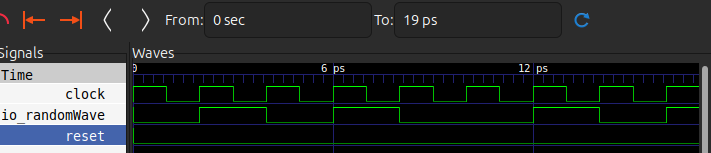
\includegraphics[width=\textwidth]{Images/verilator_waveformgenerator_screenshot.png} 
    \caption{Waveforms for generated SystemVerilog Verilator simulation}
    \label{fig:verilator_wave}
\end{figure}

Figure \ref{fig:verilator_wave} shows the waveform produced by simulating the clock generator using verilator. Section \ref{sub:verilator_test_driver} shows the process for generating the waveform shown in Figure \ref{fig:verilator_wave}. 


}%end chisel



\ifthenelse{\boolean{verilogversion} \and \boolean{chiselversion}}{   
%*********************************************************************************
\subsubsection{Comparison of Chisel and SystemVerilog Implementation of Waveforms}
%**********************************************************************************
In the Chisel implementation of the \texttt{waveFormGenerator}, the functionality is expressed using high-level abstractions. The \texttt{randomWave} is generated as a cyclic sequence of Boolean values, and its transitions are determined by a counter that increments on every clock cycle. Unlike the Verilog version, the Chisel implementation does not explicitly emulate timing delays but instead assumes uniform timing for each state in the sequence. 

While both implementations generate a \texttt{randomWave} and a clock-like signal, they differ in their timing behavior and functionality. The Verilog version explicitly specifies time delays for signal transitions and provides a clear stop condition using \texttt{\$stop}. The Chisel version is higher-level, more abstract, and assumes regular timing intervals without emulating the exact delays. This makes the Chisel version more suitable for hardware synthesis, where timing is managed by the clock, while the Verilog version offers precise control for simulation purposes.
}%end both true

%%%%%%%%%%%%%%%%%%%%%%%%%%%%%%%%%%%%%%%%%%%
\section{One-Input Combinational Circuits}
%%%%%%%%%%%%%%%%%%%%%%%%%%%%%%%%%%%%%%%%%%%
Combinational circuits are a fundamental type of digital circuit where the outputs are determined solely by the current inputs, without any memory or feedback elements. They perform logical and arithmetic operations based on Boolean algebra. Examples of combinational circuits include logic gates (AND, OR, NOT), arithmetic circuits (adders, subtractors), and data routing components (multiplexers, encoders). These circuits are deterministic, meaning their outputs are uniquely determined by the given inputs \cite{mano2017}.

%******************************
\subsection{Formal Description}
%******************************
A one-input combinational circuit is a digital logic circuit where the output depends solely on the value of a single binary input \( A \). Such circuits are governed by a Boolean function \( f(A) \), where \( f: \{0, 1\} \to \{0, 1\} \). The output is computed instantaneously based on the input value, with no memory or feedback elements involved. The behavior of the circuit can be described by a truth table, which enumerates the two possible input values (\( A = 0 \) and \( A = 1 \)) and their corresponding outputs (\( f(0) \) and \( f(1) \)). 

\begin{table}[H]
  \begin{center}
    \caption{One-input circuits.}
    \label{tab:one_input_circuits}
    \begin{tabular}{|c||c|c|c|}
      \hline
      A&  &  NOT&  BUFFER      \\ \hline \hline
      0&  &   1&       0    \\ \hline
      1&  &   0&       1    \\ \hline
    \end{tabular}
  \end{center}
\end{table}

\placedrawing[H]{figures/02_01_not.lp}{Graphic representation of the NOT and BUFFER circuits.}{fig:one_input_ckt}

Table \ref{tab:one_input_circuits} shows the truth table for a NOT gate\index{gate: logical circuit!NOT: logic circuit that inverts the truth value}, which inverts the input (\( f(A) = \neg A \)), and BUFFER (constant) circuit, which outputs a fixed value regardless of the input (\( f(A) = 0 \) or \( f(A) = 1 \)). Figure \ref{fig:one_input_ckt} shows the logic circuit symbol of the NOT and BUFFER combinational circuits. This is also called a gate symbol.

%***************************************************
\subsection{Physical Implementation of NOT Circuit}
%***************************************************
The physical implementation of a NOT circuit, or inverter, bridges the abstract concept of Boolean algebra with real-world digital hardware. A NOT gate takes a single input and produces an output that is its logical complement. In practice, this is typically achieved using transistor-based designs, such as CMOS (Complementary Metal-Oxide-Semiconductor) technology. 

The delay inherent in a NOT circuit, commonly referred to as the \emph{gate delay}, arises from the physical properties of the transistors and the interconnects. When the input changes state, the transistors must charge or discharge the capacitive load at the output. This charging and discharging process is influenced by factors such as the capacitance of the output node, the resistance of the transistors, and the speed of the power supply. As a result, the propagation delay, defined as the time taken for the output to reach a certain percentage of its final value after a change in input, becomes an important metric in digital circuit performance. 

Understanding where gate delays originate is important for designing circuits that meet timing requirements in high-speed applications. The interested reader can consult Appendix \ref{app:physical_implementations} for more information.

%%%%%%%%%%%%%%%%%%%%%%%%%%%
\section{Two-input gates}
%%%%%%%%%%%%%%%%%%%%%%%%%%%
Two-input gates depend on two binary inputs. Common two-input gates include AND, OR, XOR, NAND, and NOR. 

%*******************************
\subsection{Formal Description}
%******************************
Two-input gates are fundamental components in digital logic that perform Boolean operations on two binary variables, \( A \) and \( B \), to produce a single output \( f(A, B) \). Mathematically, these gates implement functions \( f: \{0, 1\} \times \{0, 1\} \to \{0, 1\} \), where the domain consists of all possible ordered pairs of binary inputs, and the range is restricted to binary outputs. 

Each type of two-input gate corresponds to a specific Boolean operation, such as AND (\( f(A, B) = A \land B \)). The behavior of these gates can be fully specified using truth tables, which enumerate all possible input combinations and their corresponding outputs.

\begin{table}[H]
  \begin{center}
    \caption{Two-input Combinational Gates Truth Table.}
    \label{tab:two_input_gates}
    \begin{tabular}{|c|c||c|c|c|c|c|c|}
      \hline
      $A$& $B$&   OR&        NOR&              AND&     NAND&              XOR&         XNOR \\ 
       &  &  $A\lor B$ & $\neg (A \lor B)$& $A\land B$& $\neg (A \land B)$&  $A\oplus B$&   $\neg (A \oplus B)$                              \\ \hline \hline
      0& 0&  0&         1&                 0&       1&                  0&           1\\ \hline
      0& 1&  1&         0&                 0&       1&                  1&           0\\ \hline
      1& 0&  1&         0&                 0&       1&                  1&           0\\ \hline
      1& 1&  1&         0&                 1&       0&                  0&           1\\ \hline
    \end{tabular}
  \end{center}
\end{table}

Table \ref{tab:two_input_gates} shows the truth table for combinational 2-input gates and Table \ref{tab:logic_gates_summary} shows the summary of their interpretations.

\begin{description}
\item[AND]:\index{gate: logical circuit!AND: compute the Boolean conjunction} \( A \cdot B = AB \), where \( AB = 1 \) only if both \( A \) and \( B \) are 1, otherwise \( AB = 0 \). \\
    Numerical interpretation: Arithmetic product. \\
    Symbolic interpretation:  Gate, because \( A = 1 \) opens the way for \( B \). \\
    Alternative names: Conjunction, multiply gate, all-or-nothing gate \cite{boole1854book, rosen2018}.

\item[NAND]:\index{gate: logical circuit!NAND: compute the inverse of the Boolean conjunction} \( \neg (A \cdot B) \), where the output is \( 0 \) only if both \( A \) and \( B \) are 1; otherwise, the output is \( 1 \). \\
    Symbolic interpretation: Universal gate. \\
    Alternative names: Sheffer stroke, negated AND gate \cite{sheffer1913, rosen2018}.

\item[OR]:\index{gate: logical circuit!OR: compute the Boolean disjunction} \( A + B \), where \( A + B = 1 \) if at least one of \( A \) or \( B \) is \( 1 \); otherwise, \( A + B = 0 \). \\
    Symbolic interpretation: Inclusive OR. \\
    Alternative names: Disjunction, any-or-all gate \cite{rosen2018}.

\item[NOR]:\index{gate: logical circuit!NOR: compute the inverse of the  Boolean disjunction} \( \neg (A + B) \), where the output is \( 0 \) if at least one of \( A \) or \( B \) is \( 1 \); otherwise, the output is \( 1 \). \\
    Symbolic interpretation: Universal gate. \\
    Alternative names: Peirce arrow, negated OR gate \cite{peirce1885, rosen2018}.

\item[XOR]:\index{gate: logical circuit!XOR: compute the Boolean exclusive OR} Exclusive OR, because it excludes the case \( A = B = 1 \) in determining \( 1 \) on the output. \\
    \( A \oplus B = 1 \) when only one of the inputs \( A \) or \( B \) is \( 1 \). \\
    Logic interpretation: Conditioned inverter, i.e., \( \text{if } A = 0 \text{ then } A \oplus B = B, \text{ else } A \oplus B = B' \). \\
    Numerical interpretation: Modulo-2 sum. \\
    Symbolic interpretation: Anticoincidence. \\
    Alternative names: Either-or gate, modulo-2 adder \cite{shannon48, rosen2018}.

\item[XNOR]:\index{gate: logical circuit!nXOR: compute the inverse of the Boolean exclusive OR} \( \neg (A \oplus B) \). \\
    Symbolic interpretation: Coincidence. \\
    Alternative names: Equality gate, NOT XOR \cite{mano2017, rosen2018}.
\end{description}

\begin{table}[htbp]
\centering
\renewcommand{\arraystretch}{1.5} % Adjust row height
\setlength{\tabcolsep}{5pt} % Adjust column spacing
\begin{tabular}{|>{\centering\arraybackslash}p{2cm}|>{\centering\arraybackslash}p{3cm}|>{\centering\arraybackslash}p{2cm}|>{\centering\arraybackslash}p{5cm}|}
\hline
\textbf{Logic Gate} & \textbf{Numerical} & \textbf{Symbolic} & \textbf{Alternative Names} \\ \hline

OR  & Logical addition (no carry) \( A + B \) & \( A \lor B \) & Disjunction, Any-or-All Gate, Inclusive OR \\ \hline

NOR  & Complement of OR: \( 1 - (A + B) \) & \( \neg (A \lor B) \) & Peirce Arrow, Negated OR Gate, Universal Gate \\ \hline

AND & Logical multiplication \( A \cdot B \) & \( A \land B \) & Conjunction, Multiply Gate, All-or-Nothing Gate \\ \hline

NAND  & Complement of AND: \( 1 - (A \cdot B) \) & \( \neg (A \land B) \) & Sheffer Stroke, Negated AND Gate, Universal Gate \\ \hline

XOR  & Modulo-2 addition \( A \oplus B \) & \( A \oplus B \) & Exclusive OR, Modulo-2 Adder, Anticoincidence \\ \hline

XNOR  & Complement of XOR: \( 1 - (A \oplus B) \) & \( \neg (A \oplus B) \) & Exclusive NOR, Equality Gate, Coincidence \\ \hline

\end{tabular}
\caption{Summary of Logical Gates and their Interpretations}
\label{tab:logic_gates_summary}
\end{table}

Many of the historical names in \ref{tab:logic_gates_summary} stem from different disciplines. Terms like conjunction, disjunction, and negation originate from symbolic logic. Coincidence and anticoincidence were used in early telecommunications signal processing contexts. Practical descriptions like multiply gate and modulo-2 adder reflect the role of these gates in arithmetic and data processing. Modern digital logic has largely standardized the terms AND, OR, XOR, etc., as defined by IEEE and other standard bodies \cite{ieee_std_91}.

\placedrawing[H]{figures/02_07_two_input_gates.lp}{Graphical representation of the most used two-input gates.}{fig:graphical_gates}
Figure \ref{fig:graphical_gates} shows the graphical representations of logic gates. These originated from the need to visually depict logical operations in a way that facilitated the design and analysis of digital systems. These representations were inspired by symbolic logic and Boolean algebra, where logic functions were expressed using abstract symbols. Early pioneers, such as Claude Shannon, formalized the connection between Boolean algebra and electronic circuits, enabling the translation of logical expressions into circuit designs \cite{shannon48}. Over time, distinct shapes were assigned to each gate for clarity—such as the triangular symbol for NOT gates and the curved line for OR gates. Standardization efforts by organizations like the IEEE and IEC later codified these symbols, ensuring universal recognition and consistency in circuit diagrams \cite{ieee_std_91}. 


\placedrawing[H]{figures/02_08_non_inverting_gate_waveforms.lp}{Waveforms for the non-inverting gates.}{fig:waveforms}
Waveforms are tools used in digital logic for visualizing and analyzing the behavior of signals over time. They represent the changes in voltage levels for inputs, outputs, and intermediate nodes in a circuit, making it easier to understand timing relationships, transitions, and delays. The use of waveforms emerged alongside the development of oscilloscopes and other signal measurement tools in the early 20th century, as engineers needed a method to observe electrical signals in real-time. With the advent of digital systems, waveforms became a standard way to represent binary signals, where high and low voltage levels correspond to logical 1s and 0s, respectively. Waveforms allow engineers to verify the correct operation of logic circuits and diagnose timing-related issues such as glitches, race conditions, and setup/hold violations \cite{horowitz1993, ieee_waveform}. Their graphical nature complements schematic diagrams by providing temporal information that is not inherently visible in static circuit representations.


Figure \ref{fig:waveforms} shows the behavior of AND, OR and XOR gates. They are driven by the signals $A$ and $B$ represented in the first two wave forms. Besides the logic response to the inputs, timing characteristics are also shown. 
\begin{itemize}
    \item $t_+$: the positive transition time (the duration of the positive edge)
    \item $t_-$: the negative transition time (the duration of the negative edge)
    \item $t_{pLH}$: the propagation time  of the signal through the gate for the transition from Low to High
    \item $t_{pHL}$: the propagation time  of the signal through the gate for the transition from High to Low
\end{itemize}

We leave the treatment of timing to a course on digital logic design. It is a critical component in building working systems but is abstracted away in this book.

%%%%%%%%%%%%%%%%%%%%%%%%%%%
\section{Many-Input Gates}
%%%%%%%%%%%%%%%%%%%%%%%%%%%
Many-input gates are a generalization of 2-input gates, allowing the combination of more than two inputs into a single logical operation. For instance, an \( n \)-input AND gate outputs a logical \( 1 \) only when all \( n \) inputs are \( 1 \), while an \( n \)-input OR gate outputs \( 1 \) when at least one of the inputs is \( 1 \). As the number of inputs increases, the complexity of the gate's behavior grows exponentially, based on the number of possible input configurations.

Mathematically, the total number of distinct \( n \)-input gates is \( N^{2^n} \), where \( N \) represents the number of possible output values (typically \( N = 2 \) for binary logic), and \( 2^n \) is the total number of unique input configurations for \( n \) inputs. This exponential growth means that even for relatively small \( n \), the number of possible logic gates becomes vast and impractical to enumerate. For example, with \( n = 3 \), there are \( 2^{2^3} = 256 \) possible gates. For \( n > 2 \), Boolean algebra rules are necessary for simplifying and managing these functions, enabling the design of practical circuits without explicitly listing all possible gates.

In modern digital design, many-input gates are often implemented using a combination of smaller gates, as direct implementation can become physically and computationally impractical for large \( n \). For example, a 16-input AND gate might be constructed hierarchically by combining multiple 2-input AND gates. 

Let us consider some significant examples using verilog's' (tick) symbol to denote negation:

\begin{itemize}
    \item (A')' = A
    \item AB + AB' = A(B + B') = A $\cdot$ 1 = A\\
    When B=1 the expression takes the value A, and when B=0 the expression still takes the value A, we conclude that the value of B does not matter and the expression takes the value A.
    \item A + A'B = A + B\\
    This can be proved by the truth table in Table \ref{tab:truth_table_proof}.
    \begin{table}[H]
  \begin{center}
    \caption{Truth table proof of A + A'B = A + B.}
    \label{tab:truth_table_proof}
    \begin{tabular}{|c|c||c|c|c||c|}
      \hline
      A& B&  A'& A'B& A+A'B& A+B   \\ \hline \hline
      0& 0&   1&   0&     0&   0   \\ \hline
      0& 1&   1&   1&     1&   1   \\ \hline
      1& 0&   0&   0&     1&   1   \\ \hline
      1& 1&   0&   0&     1&   1   \\ \hline
    \end{tabular}
  \end{center}
\end{table}
    \item A $\oplus$ B = (A' $\oplus$ B)' = (A $\oplus$ B')' = A' $\oplus$ B'
    \item A + B = (A'B')' \\
    From de Morgan's rule, A or B is 1 is equivalent to the fact that it is not true that A is 0 and B is 0.
    \item AB = (A' + B')'\\
    From de Morgan rule, A and B are 1 is equivalent to the fact that it is not true that A is 0 or B is 0.
\end{itemize}


%%%%%%%%%%%%%%%%%%%%%%%%%%%%%%%%%%%%%%%%%%%%%%%%%%%%%%%%%%%%%%%%%%%%%%%%%%%%%%%%%%%%%%%%%%%%%%%%%%%
\section{Generic combinational circuits}
%%%%%%%%%%%%%%%%%%%%%%%%%%%%%%%%%%%%%%%%%%%%%%%%%%%%%%%%%%%%%%%%%%%%%%%%%%%%%%%%%%%%%%%%%%%%%%%%%%%

\placedrawing[H]{figures/02_09_decoder.lp}{Decoder with $n$-bit input (DCDn).}{fig:decoder}

%*******************
\subsection{Decoder}
%********************
Figure \ref{fig:decoder} shows a generic $n$-bit {\bf {\em decoder}}\index{decoder: logic circuit that translates a binary-encoded input signal into a unique one-hot output}. A decoder is a combinational logic circuit that translates a binary-encoded input signal into a unique {\bf {\em one-hot}}\index{one-hot: a representation in which only one bit is set to '1', while all other bits are '0'} output. The term "one-hot" refers to a representation in which only one bit is set to '1', while all other bits are '0'. For example, in a 4-bit 1-hot code, valid outputs include 0001, 0010, 0100, and 1000. This encoding is commonly used in digital systems for control logic. It eliminates the need to decode multiple bits simultaneously. 

\begin{figure}[h!]
\centering
\[
\begin{array}{|c|c||c|c|c|c|}
\hline
\text{Input} & \text{Input} & \text{Output} & \text{Output} & \text{Output} & \text{Output} \\
x_1 & x_0 &  y_3 &  y_2 & y_1 & y_0 \\
\hline
0 & 0 & 0 & 0 & 0 & 1 \\
0 & 1 & 0 & 0 & 1 & 0 \\
1 & 0 & 0 & 1 & 0 & 0 \\
1 & 1 & 1 & 0 & 0 & 0 \\
\hline
\end{array}
\]
\caption{Truth table for a 2-to-4 decoder. Each input combination activates one unique output in a one-hot encoding scheme.}
\label{fig:decoder_truth_table}
\end{figure}

\placedrawing[H]{figures/02_10_recursive_decoder.lp}{Recursively defined 3-input decoder (DCD). {\bf a.} Elementary decoder (eDCD). {\bf b.} Two-input decoder (DCD2). {\bf c.} Three-input DCD (DCD3).}{fig:decoder_and_gates}

A decoder takes an \(n\)-bit binary input and generates \(2^n\) output lines, with exactly one line active (logic high) for any given input combination. The structure of a decoder includes an array of logic gates that process the input bits and their complements to generate the appropriate output signals. For example, Figure \ref{fig:decoder_truth_table} shows the truth table for a 2-to-4 decoder. Figure \ref{fig:decoder_and_gates}a shows an elementary decoder\index{elementary decoder: a one-input decoder} that outputs both $x_n$ and $\overline{x_n}$. Figure \ref{fig:decoder_and_gates}a shows that the two input bits (\(x_1\) and \(x_0\)) and their negations (\(\overline{x_0}\) and \(\overline{x_1}\)) are used to drive four output signals (\(y_3, y_2, y_1, y_0\)). 



Decoders are widely used in digital systems for applications such as memory addressing, instruction decoding in processors, and enabling control signals in multiplexers. 


%#######################
% Decoder Code
%#######################
\ifthenelse{\boolean{verilogversion}}{
%*********************************************************
\subsubsection{Decoder (SystemVerilog)}
%*********************************************************    
\includeverilogcode[caption={Parameterized Decoder (SystemVerilog: dcdParameterized.sv)},     label={lst:verilog_decoder_parameterized}, firstline=2, firstnumber=1, lastline=999]{\verilogSourceDir/dcdParameterized.sv}

Listing \ref{lst:verilog_decoder_parameterized} shows a parameterized decoder implemented in SystemVerilog, which provides a scalable solution for decoding binary inputs to a one-hot encoded output. The design uses the shift operation to map the binary input to a specific bit position in the output. By using the parameter \texttt{INPUT\_WIDTH}, the module can dynamically adjust the size of the binary input and its corresponding one-hot output, with the output width automatically calculated as \(2^{\texttt{INPUT\_WIDTH}}\). This ensures that the decoder is flexible and reusable across various designs.

The key operation in the decoder is the left shift, expressed as \texttt{out = 1'b1 << in}, where the binary input \texttt{in} determines how many positions the single high bit is shifted. This eliminates the need for case statements or nested conditional logic. The shift operation is synthesis-friendly, allowing hardware tools to map the logic to a simple decoder circuit directly. 

\includeverilogcode[caption={4-to-16 Behavioral Decoder (SystemVerilog:dcd.sv)},     label={lst:verilog_decoder_4_to_16}, firstline=2, firstnumber=1, lastline=999]{\verilogSourceDir/dcd.sv}

Listing \ref{lst:verilog_decoder_4_to_16} shows a directly implemented 4-to-16 decoder.

}% End Verilog

\ifthenelse{\boolean{chiselversion}}{
%*************************************************
\subsubsection{Decoder (Chisel)}
%*************************************************
\includechiselcode[caption={Parameterized Decoder (Chisel: Decoder.scala)}, label={lst:chisel_decoder}, firstline=9, firstnumber=9, lastline=999]{\chiselSourceDir/Decoder.scala}

Listing \ref{lst:chisel_decoder} shows a Chisel parameterized decoder that can generate decoder logic based on a specified width. The decoder accepts a parameter, \texttt{n} the output width. This is also used to determine the number of input bits using the function \texttt{log2Ceil(n)}. This parameter dynamically adjusts the size of the output vector to \texttt{1 << inputWidth} (i.e., $2^{\text{inputWidth}}$), allowing the decoder to handle a variable number of input combinations. The use of a shift operation, \texttt{1.U << io.in}, implements the decoding logic by setting a single output bit corresponding to the binary input value.

\includechiselcode[caption={Instantiated 2-to-4 Decoder (Chisel: Decoder2to4.scala)}, label={lst:chisel_2to4_decoder}, firstline=8, firstnumber=8, lastline=999]{\chiselSourceDir/Decoder2to4.scala}

Listing \ref{lst:chisel_2to4_decoder} line 8 shows how simple it is to instantiate a decoder of any output width.

\includeverilogcode[caption={SystemVerilog Generated for Chisel firtool Decoder(4)}, label={lst:chisel_decoder_generated_verilog}, firstline=1, firstnumber=1, lastline=9999]{\verilogGeneratedByChiselSourceDir/Decoder2to4.v}

Chisel (or more precisely, firtool) automatically generates SystemVerilog for parameterized modules, while guaranteeing combinational logic. Listing \ref{lst:chisel_decoder_generated_verilog} shows the generated verilog code for a 2-to-4 decoder \texttt{Decoder(4)}.

\includeverilogcode[caption={Verilog Generated by sv2v for Decoder(4)}, label={lst:sv2v_decoder_generated_verilog}, firstline=1, firstnumber=1, lastline=9999]{\verilogGeneratedBySvtovSourceDir/Decoder2to4.v}

Commercial tools such as Vivado can directly elaborate and synthesize SystemVerilog. yosys, an open-source tool, can elaborate and synthesize some SystemVerilog statements but not all of them. We convert SystemVerilog to pure verilog using the open-source sv2v tool. Listing \ref{lst:sv2v_decoder_generated_verilog} line 11 shows that the shift semantics of the decoder are preserved in the generated verilog.

\includeverilogcode[caption={Verilog Elaborated by yosys for Decoder(4)}, label={lst:yosys_decoder_generated_verilog}, firstline=1, firstnumber=1, lastline=9999]{\verilogGeneratedByYosysSourceDir/Decoder2to4.v}

Listing \ref{lst:yosys_decoder_generated_verilog} shows the elaborated verilog produced by yosys. The shift operation has been transformed into logical operations. Lines 18 through 21 show the elaboration.

\begin{figure}[H]
    \centering
    \includegraphics[width=0.8\textwidth]{\diagramsDir/Decoder2to4.png} 
    \caption{Generated Schematic of a yosys synthesized Chisel 2-to-4 Decoder.}
    \label{fig:ckt-2to4-decoder} % Use a label for cross-referencing
\end{figure}

After being elaborated by yosys, the schematic of \ref{fig:ckt-2to4-decoder} is automatically generated by netlistsvg.

}%End Chisel


\ifthenelse{\boolean{verilogversion} \and \boolean{chiselversion}}{   
%*********************************************************************************
\subsubsection{Decoder Language Comparison}
%**********************************************************************************

Chisel is a hardware construction language that generates hardware descriptions (e.g., Verilog) through the execution of Scala code. Its parameterized decoder uses functional programming paradigms to adjust the number of output bits based on the input width. The parameterized \texttt{Decoder} in Chisel is evaluated at \textbf{generation time}, which corresponds to the compile time of the Scala program, not the hardware synthesis. When the Chisel code is executed, the Scala runtime evaluates the parameterization and generates the corresponding Verilog/SystemVerilog code. This generated Verilog/SystemVerilog is then synthesized into hardware, meaning the parameterization is resolved before hardware runtime and does not exist dynamically in the final design.

Verilog lacks native parameterization and higher-level constructs, making it less flexible for scalable designs. A typical Verilog decoder implementation relies on manual enumeration or explicit assignment of output bits using case statements or combinational logic. 

SystemVerilog, as an enhancement of Verilog, introduces parameterization capabilities, which allow developers to create reusable and configurable hardware modules. A parameterized module in SystemVerilog uses \texttt{parameter} and \texttt{generate} constructs. Additionally, SystemVerilog supports advanced constructs like \texttt{logic} and \texttt{always\_comb}, which enforce combinational behavior. SystemVerilog parameterized designs are evaluated at \textbf{synthesis time}, when the hardware description is compiled and mapped into a physical implementation. These constructs allow for flexible and static parameterization, which the synthesis tool resolves before producing the final hardware netlist. 
}% End Both


%%%%%%%%%%%%%%%%%%%%%%%%
\subsection{Multiplexer}\label{genericMux}
%%%%%%%%%%%%%%%%%%%%%%%%%

A {\bf {\em multiplexer}}\index{multiplexer: selects one of several input signals according to a selection code} (often abbreviated \textit{mux}) is a combinational logic circuit that selects one of several input signals and transmits the selected input to a single output line. The input selection is controlled by a set of control signals or \textit{select lines} that determine which input to pass to the output. A multiplexer with $n$ select lines can control the $2^n$ inputs, making it a highly versatile and compact solution for signal routing in digital systems.

Multiplexers are widely used in digital design due to their ability to manage multiple signals within a system efficiently. In arithmetic circuits, multiplexers are often used for operations such as selecting between different data sources or routing data to various processing units. They are also important components in larger systems, such as CPUs, where they help implement control logic, ALU operation selection, and pipeline data forwarding. For example, in a microprocessor, a multiplexer might be used to select between input operands for an arithmetic operation based on the current instruction.

Multiplexers are used because they minimize the number of physical connections and wires required in a circuit. By reducing the need for separate connections for each input-output pair, a multiplexer allows for more efficient circuit designs. In addition, they enhance the scalability of systems because additional inputs can be accommodated by increasing the number of select lines. 

%**********************************
\subsection{Elementary Multiplexer}
%**********************************

Any combinational circuit can be expressed using only NAND functions. But a more interesting "fundamental brick" could be a circuit corresponding to the ubiquitous {\bf {\em if-then-ellse}} statement. It is the elementary multiplexer\index{elementary multiplexer: a 2 selected inputs multiplexer} (eMUX) represented in Figure \ref{fig:mux}, and shows the following:

\placedrawing[H]{figures/02_11_mux.lp}{Elementary multiplexer (eMUX). {\bf a.} The circuit structure: an eDCD serially connected with an AND-OR circuit. {\bf b.} The logic symbol.}{fig:mux}


\begin{center} O = {\bf if} (S) {\bf then} I1 {\bf else} I0 \end{center}

%**********************************
\subsection{Many-input Multiplexer}
%**********************************

Figure \ref{fig:gen_mux} shows a multiplexer with many-inputs. It takes bits from $m=2^n$ inputs selected by a $n$-bit code.

\placedrawing[H]{figures/02_12_mux_generalized.lp}{The general definition of the multiplexer circuit (MUXn). {\bf a.} The structure of MUXn: a DCDn serially connected with a $m=2^n$ ANDs on the first level of an AND-OR structure. {\bf b.} The logic symbol for MUXn.}{fig:gen_mux}

%#######################
% Multiplexer Code
%#######################
\ifthenelse{\boolean{verilogversion}}{
%*********************************************************
\subsubsection{Multiplexer (SystemVerilog)}
%*********************************************************    


Listing \ref{lst:verilog_mux4} implements a 16-to-1 single bit multiplexer. The module takes three inputs: a 16-bit vector \texttt{muxIn}, a 4-bit selector \texttt{muxSel}, and produces a single 1-bit output \texttt{muxOut}. The selector \texttt{muxSel} determines which bit of the 16-bit input vector is routed to the output. This is achieved through the indexing operation \texttt{muxIn[muxSel]}, which dynamically selects the bit of \texttt{muxIn} corresponding to the value of \texttt{muxSel}.

\includeverilogcode[caption={16-to-1 single bit Multiplexer (SystemVerilog: mux.sv)},     label={lst:verilog_mux4}, firstline=2, firstnumber=1, lastline=999]{\verilogSourceDir/mux.sv}

This design is both compact and efficient, leveraging Verilog's built-in array indexing capabilities. It allows the multiplexer to be easily scaled by adjusting the widths of \texttt{muxIn} and \texttt{muxSel}. Such multiplexers are fundamental building blocks in digital systems, often used to select between multiple data sources or routes in logic circuits, enabling dynamic and efficient data flow management.
}% End Verilog Code

\ifthenelse{\boolean{chiselversion}}{
%*************************************************
\subsubsection{Parameterized Bus Multiplexer (Chisel)}
%*************************************************
A \textit{bus} in digital systems is a collection of parallel lines or pathways used to transfer data between components within a system. Each line in a bus corresponds to a bit in the data, allowing the bus to carry multi-bit data simultaneously. Buses are parameterized by their width, which determines how many bits can be transmitted at once, and are used to connect various hardware components, such as processors, memory, and peripherals. For example, a 32-bit bus can carry 32 bits of data in parallel. 

\includechiselcode[caption={Parameterized Bus Type Multiplexer (Chisel: MultiplexerGenericType.scala)}, label={lst:chisel_muxT}, firstline=9, firstnumber=9, lastline=9]{\chiselSourceDir/MultiplexerGenericType.scala}


\addcontentsline{toc}{paragraph}{gen vs dataType - Chisel} \index{Chisel!gen} \index{Chisel!dataType}
Listing \ref{lst:chisel_muxT} shows a parameterized bus multiplexer in Chisel where the type of the bus is also parameterized using \texttt{[T <: Data](gen: T)]}. In Chisel, parameterizing modules with type parameters is a common practice to create reusable and modular designs. The choice between using \texttt{gen} and \texttt{dataType} depends on the context and the semantics of the module being designed. Each serves a slightly different purpose depending upon the intended hardware abstraction.

The \texttt{gen} parameter is well-suited when the type represents a \textit{blueprint} for generating multiple hardware elements. This is particularly relevant in cases where the module processes or instantiates multiple instances of the same type, such as multiplexers or reusable modules like FIFO queues and bus interfaces. For example, in Listing \ref{lst:chisel_muxT}, a multiplexer uses \texttt{gen} to define the type of data inputs and outputs, emphasizing that multiple identical instances are being handled within the hardware structure. 

 Given scala's generic types and type checking capabilities, it would be desirable to parameterize the bus type. Unfortunately, when generating hardware, this can sometimes appear as an invalid type conversion even if all interfaces are instantiated with \texttt{UInt<>}. Therefore, \textbf{ \textit{in this book, we have specified all classes to use \texttt{UInt}. This more closely aligns to verilog wires. }}Where possible, inside implementations, we still strive to ensure type safety using conversions such as \texttt{.asBool} and \texttt{.asSInt}, etc. 

\includechiselcode[caption={Parameterized Bus Width Multiplexer (Chisel: Multiplexer.scala)}, label={lst:chisel_mux}, firstline=9, firstnumber=9, lastline=20]{\chiselSourceDir/Multiplexer.scala}

Listing \ref{lst:chisel_mux} shows a bus multiplexer implemented as a class named \texttt{class Multiplexer}. This class is parameterized by the number of inputs (\texttt{n}) and the width of the bus (\texttt{width}). As shown on lines 14 through 16, all inputs and outputs are of type \texttt{UInt}  The class ensures through \texttt{require} statements that the number of inputs is both greater than zero and a power of two. 

The I/O bundle defines the interface for the multiplexer. It includes a vector (bus) of inputs, a selection signal, and the output. The size of the selection signal is calculated using \texttt{log2Ceil}, ensuring that it has enough bits to address all the inputs. The core logic of the multiplexer is implemented in a single line \texttt{io.output := io.inputs(io.select)}, where the output is assigned the value of the selected input. This is performed using Chisel’s vector indexing.

In Scala, a companion object is an object that shares the same name as a class and is defined in the same file. It acts as a singleton instance and provides a convenient way to group static-like methods and values associated with the class. Companion objects are particularly useful for factory methods, constants, or utility functions related to the class. Since they are in the same scope, companion objects and their corresponding classes can access each other's private members. This feature allows Scala developers to maintain clean and organized code, while still supporting the functional programming paradigm by avoiding the need for static members like in Java.

\includechiselcode[caption={Parameterized Bus Width Multiplexer Companion Object (Chisel: Multiplexer.scala)}, label={lst:chisel_mux_companion}, firstline=22, firstnumber=22, lastline=30]{\chiselSourceDir/Multiplexer.scala}

Listing \ref{lst:chisel_mux_companion} shows the companion object. The \texttt{Multiplexer} \textit{object} provides a factory method for creating and connecting instances of a parameterized multiplexer. The method takes a \texttt{Vec[UInt]} of inputs, and a \texttt{UInt} that specifies the selection signal for the multiplexer. After the module is instantiated, its I/O ports are connected. The \texttt{mux.io.inputs} port is connected to the \texttt{inputs} vector, and the \texttt{mux.io.select} port is connected to the \texttt{select} signal. Finally, the \texttt{apply} method returns the \texttt{mux.io.output}, providing the result of the multiplexer to the caller. 

\includechiselcode[caption={4-to-1 8-bit Bus Multiplexer (Chisel: Mux4.scala)}, label={lst:chisel_mux4}, firstline=8, firstnumber=8, lastline=999]{\chiselSourceDir/Mux4.scala}

Listing \ref{lst:chisel_mux4} shows an instantiation of a multiplexer with four 8-bit inputs. It uses the companion object to connect the signals. If the I/O signals retain the same names as the Multiplexer class, the 4-to-1 8-bit bus multiplexer could have been instantiated the same way as the 2-to-4 decoder shown in Listing \ref{lst:chisel_2to4_decoder} - \texttt{class Mux4 extends Multiplexer(4)}. However, it is often more convenient for users of hardware libraries to see the I/O definitions in the leaf class. Generally, we try to follow this design principle for instantiated Chisel hardware and so Listing \ref{lst:chisel_mux4} fully specifies the I/O signals.

\begin{figure}[H]
    \centering
    \includegraphics[width=0.6\textwidth]{\diagramsDir/Mux4.png} 
    \caption{Generated Schematic of a yosys Elaborated Chisel 4-to-1 Multiplexer.}
    \label{fig:mux4} 
\end{figure}

Figure \ref{fig:mux4} shows the hierarchical schematic after yosys elaboration.

\begin{figure}[H]
    \centering
    \includegraphics[scale=0.23]{\diagramsDir/Mux4_flat.png} 
    \caption{Generated Schematic of a yosys Elaborated and Flattened Chisel 4-to-1 Multiplexer.}
    \label{fig:mux4_flat} 
\end{figure}

Figure \ref{fig:mux4_flat} shows the schematic after the elaborated design is flattened. It is built from multiple 2-to-1 multiplexers.

}% End Chisel Code

%%%%%%%%%%%%%%%%%%%%%%%%%%%
\subsection{Demultiplexer}
%%%%%%%%%%%%%%%%%%%%%%%%%%%
A {\bf {\em demultiplexer}}\index{demultiplexer: channels a one-bit input into one of several output lines based on  a selection signal}, often abbreviated as "demux," is a combinational circuit that takes a single input and channels it into one of several output lines based on the value of a selection signal. It is effectively the reverse operation of a multiplexer, consolidating multiple inputs into a single output. A demultiplexer is characterized by its ability to control the routing of the input data to the desired output line, ensuring that only one output is active at a time. The selection signal's binary value governs the active output selection.

Demultiplexers are useful in digital systems for tasks that require data distribution. For example, they are used in scenarios where a single source of information needs to be directed to one of many destinations. In data routing applications, demultiplexers help reduce the complexity of data paths and enable efficient communication between components. Moreover, they are integral to memory addressing systems, where they are used to select specific memory locations for reading or writing operations.

\placedrawing[H]{figures/02_13_demux.lp}{Demultiplexer as a DCD whose outputs are ANDed with the one bit signal to be distributed according to the $n$-bit input code. }{fig:demux}

Figure \ref{fig:demux} shows the demultiplexer that transfers the input signal X to one of the $m=2^n$ outputs, $y_0, y_1, \ldots, y_{m-1}$, indicated by the $n$-bit selection input, $x_0, x_1, \ldots, x_{n-1}$. In Figure \ref{fig:demux} a demultiplexer is built using a decoder which opens only one of the $m$ AND gates sending the $X$ input to the selected output.

For example: if $$\{x_{n-1} x_{n-2}, \ldots, x_1, x_0\} = 00 \ldots 011$$ then
$$\{y_{m-1} y_{m-2} \ldots y_0 y_1\} = 00 \ldots 0X000$$

%#######################
% DeMltiplexer Code
%#######################
\ifthenelse{\boolean{verilogversion}}{
%*********************************************************
\subsubsection{Demultiplexer (SystemVerilog)}
%*********************************************************   

Listing \ref{lst:verilog_demux16} shows SystemVerilog code that implements a simple demultiplexer module, named \texttt{dMux}. This demultiplexer takes a input signal \texttt{dMuxEnable} and routes one-bit of it to one of the 16 output lines, represented by the vector \texttt{dMuxOut}, based on the 4-bit selection signal \texttt{dMuxIn}. Instead of left-shifting the number 1 as in the decoder, the one-bit value $X$ is left-positioned. The operation is performed using a left-shift operation, where the input signal \texttt{dMuxEnable} is shifted by the value of \texttt{dMuxIn}, effectively enabling only one bit in the 16-bit output vector.

\includeverilogcode[caption={1-to-16 bit Demultiplexer (SystemVerilog: dMux.sv)}, label={lst:verilog_demux16}, firstline=2, firstnumber=1, lastline=999]{\verilogSourceDir/dMux.sv}



The \texttt{dMuxEnable} input acts as a control signal, ensuring that no outputs are active when it is low. 

}% End Verilog Code

\ifthenelse{\boolean{chiselversion}}{
%*************************************************
\subsubsection{Parameterized Demultiplexer (Chisel)}
%*************************************************
\includechiselcode[caption={Parameterized Bus Demultiplexer (Chisel: Demultiplexer.scala)}, label={lst:chisel_demuxT}, firstline=9, firstnumber=9, lastline=999]{\chiselSourceDir/Demultiplexer.scala}

Listing \ref{lst:chisel_demuxT} shows a parameterized demultiplexer (demux) that can handle an arbitrary number of outputs of type \texttt{Vec[UInt]}. The \texttt{Demultiplexer} class that extends Chisel's \texttt{Module} class to create a hardware module. The module includes a requirement that the number of outputs must be a power of two, enforced by the \texttt{require} statement. 

The \texttt{io} bundle defines the interface for the module, consisting of an input signal of type \texttt{UInt(width.W)}, a selection signal of width \(\log_2(\texttt{numOutputs})\), and a vector of \texttt{numOutputs} output signals. The implementation defaults all output signals to zero using \texttt{foreach}, ensuring that only the selected output is driven by the input signal. This is achieved by indexing the output vector with the \texttt{select} signal, which determines the active output line.

Simlar to the Multiplexer, a companion object provides a convenient factory method for instantiating the demultiplexer. The \texttt{apply} method creates an instance of the \texttt{Demultiplexer} class and connects the provided input and selection signals to the instance's IO ports. 

\includechiselcode[caption={1-to-16 64-bit Bus Demultiplexer (Chisel: DeMux16.scala)}, label={lst:chisel_demux16}, firstline=9, firstnumber=9, lastline=999]{\chiselSourceDir/DeMux16.scala}

Listing \ref{lst:chisel_demux16} shows a \texttt{DeMux16} class that defines a 1-to-16 demultiplexer that operates on 64-bit buses. This module is implemented as a subclass of \texttt{Module}, making it a Chisel hardware component. Its interface, specified by the \texttt{io} bundle, includes a 64-bit input bus (\texttt{io.input}), a 4-bit selection signal (\texttt{io.select}) to determine the active output, and a vector of 16 output buses (\texttt{io.outputs}), each 64 bits wide. The selection signal uses a 4-bit width because \(\log_2(16) = 4\), allowing indexing of the 16 outputs.

The \texttt{DeMux16} class instantiates a parameterized demultiplexer from the \texttt{Demultiplexer} companion object. The input and selection signals (\texttt{io.input} and \texttt{io.select}) are passed as arguments to the \texttt{Demultiplexer} factory method, which returns a vector of 16 outputs. These outputs are directly assigned to \texttt{io.outputs}, ensuring that only the selected output is driven by the input signal, while the others remain zero.

}% End Chisel

%*********************************
\subsection{Seven-Segment Display}
%*********************************
A 7-segment display is a common example of a combinational circuit that illustrates the concept of many-input logic gates. It consists of seven individual segments, labeled a through g, which can be illuminated to form numerical digits (0–9). The control logic for a 7-segment display is designed as a combinational circuit that takes a binary-coded decimal (BCD) input, typically 4 bits, and determines which segments should be activated to display the corresponding digit. Each segment is controlled by a Boolean expression derived from the binary input, effectively making the display a complex multi-input gate. The circuit highlights how combinational logic can efficiently decode binary input into human-readable visual representations.

\placedrawing[H]{figures/01_03_7seg.lp}{Trans-coder for seven-segment display. }{fig:7_segment_display}

Figure \ref{fig:7_segment_display} shows the transcoder for a 7-segment display. It receives four-bit coded decimal numbers, 0 to 9, and converts them into 7-bit codes, a to g, indicating the segments to be activated, according to Table \ref{tab:sevenSeg}.

The logic expression for the output {\tt a} is the following:
\begin{center}
$a =   B'_3 \cdot B'_2 \cdot B'_1\cdot B'_0  + B'_3 \cdot B'_2 \cdot B_1\cdot B'_0  +
        B'_3 \cdot B'_2 \cdot B_1\cdot B_0  + B'_3 \cdot B_2 \cdot B'_1\cdot B_0  + $ \\
        $B'_3 \cdot B_2 \cdot B_1\cdot B'_0  + B'_3 \cdot B_2 \cdot B_1\cdot B_0  +
        B_3 \cdot B'_2 \cdot B'_1\cdot B'_0  + B_3 \cdot B'_2 \cdot B'_1\cdot B_0  $
\end{center}
or a simpler version by negating the negated function:
$$a =  (a')' =  (B'_3 \cdot B'_2 \cdot B'_1\cdot B_0  + B'_3 \cdot B_2 \cdot B'_1\cdot B'_0)' = (B'_3 \cdot B'_1 \cdot (B_2 \oplus B_0))' = B_3 + B_1 + (B_2 \oplus B_0)'$$



\begin{table}[H]
  \begin{center}
    \caption{Seven-segment display truth table.}
    \label{tab:sevenSeg}
    \begin{tabular}{|c||c|c|c|c||c|c|c|c|c|c|c|}
      \hline
     & $B_3$ & $B_2$ & $B_1$ & $B_0$ & a & b & c & d & e & f & g \\ \hline \hline
     0& 0 & 0 & 0 & 0 & 1 & 1 & 1 & 1 & 1 & 1 &   \\ \hline % 0
     1& 0 & 0 & 0 & 1 &    & 1 & 1 &    &    &    &   \\ \hline % 1
     2& 0 & 0 & 1 & 0 & 1 & 1 &    & 1 & 1 &    & 1 \\ \hline % 2
     3& 0 & 0 & 1 & 1 & 1 & 1 & 1 & 1 &    &    & 1 \\ \hline % 3
     4& 0 & 1 & 0 & 0 &    & 1 & 1 &    &    & 1 & 1 \\ \hline % 4
     5& 0 & 1 & 0 & 1 & 1 &    & 1 & 1 &    & 1 & 1 \\ \hline % 5
     6& 0 & 1 & 1 & 0 & 1 &    & 1 & 1 & 1 & 1 & 1 \\ \hline % 6
     7& 0 & 1 & 1 & 1 & 1 & 1 & 1 &    &    &    &   \\ \hline % 7
     8& 1 & 0 & 0 & 0 & 1 & 1 & 1 & 1 & 1 & 1 & 1 \\ \hline % 8
     9& 1 & 0 & 0 & 1 & 1 & 1 & 1 & 1 &    & 1 & 1 \\ \hline % 9
    \end{tabular}
  \end{center}
\end{table}

%#######################
% 7 Segment Display Code
%#######################
\ifthenelse{\boolean{verilogversion}}{
%*********************************************************
\subsubsection{Seven Segment Display (SystemVerilog)}
%*********************************************************    
\includeverilogcode[caption={Seven Segment Display (SystemVerilog: SevenSegmentDisplay.sv)},     label={lst:verilog_sevensegmentdisplay}, firstline=2, firstnumber=1, lastline=999]{\verilogSourceDir/SevenSegmentDisplay.sv}

Listing \ref{lst:verilog_sevensegmentdisplay} shows SystemVerilog code that implements a seven-segment display decoder. The module, named \texttt{sevenSegmDys}, has a 4-bit binary input, \texttt{number}, and a 7-bit output, \texttt{seg}, which controls the state of the seven segments (labeled a through g) of the display. 

The \texttt{always\_comb} block defines a combinational block that describes the behavior of the output of the circuit as a combination based on the value of the input variables. The blocking assignment, {\tt =}, is used to assure the combinational behavior.

The \texttt{case} statement maps each possible input value (0 through 9) to a corresponding 7-bit output pattern that activates the appropriate segments to display the digit. For example, the binary input \texttt{4'b0000} (decimal 0) results in the output \texttt{7'b1111110}, which lights up all segments except \texttt{g}, forming the number 0 on the display.

The module includes a \texttt{default} case that sets all segments to off (\texttt{7'b0000000}) for invalid inputs outside the range 0–9. By mapping each input to a fixed segment configuration, this module can be integrated into larger digital systems that require visual representation of numeric values, such as timers, calculators, or embedded control systems.
}%End SystemVerilog

\ifthenelse{\boolean{chiselversion}}{
%*************************************************
\subsubsection{Seven Segment Display (Chisel)}
%*************************************************
\includechiselcode[caption={Seven Segment Display (Chisel: SevenSegmentDisplay.scala)},     label={lst:chisel_sevensegmentdisplay}, firstline=8, firstnumber=8, lastline=999]{\chiselSourceDir/SevenSegmentDisplay.scala}

Listing \ref{lst:chisel_sevensegmentdisplay} shows the \texttt{SevenSegmentDisplay} class is a Chisel module that decodes a 4-bit binary input (\texttt{binIn}) into a 7-bit output (\texttt{segOut}) representing the activation of segments on a seven-segment display. The input, \texttt{binIn}, can take values from 0 to 9, and the module determines which segments (labeled \texttt{a} through \texttt{g}) should be illuminated to form the corresponding numeric digit on the display.

The \texttt{suggestName} method in Chisel provides a mechanism to assign meaningful, user-defined names to intermediate signals or wires within a hardware design. By default, Chisel generates arbitrary names for these components, which can make debugging and analyzing generated hardware descriptions (e.g., Verilog or FIRRTL) challenging. Using \texttt{suggestName}, designers can explicitly label signals with descriptive names that convey their purpose or function within the design, making the generated hardware more readable and easier to trace.

The decoding logic is implemented using a series of \texttt{when} and \texttt{elsewhen} constructs. Each condition compares \texttt{binIn} with a specific value and assigns a 7-bit binary pattern to \texttt{segOut}. Each bit in the pattern corresponds to one of the seven segments, where a \texttt{1} turns the segment on, and a \texttt{0} turns it off. For example, when \texttt{binIn} is \texttt{0}, the output is \texttt{1111110}, which activates all segments except \texttt{g} to display the digit \texttt{0}. Similarly, for \texttt{binIn = 8}, all segments are activated (\texttt{1111111}). A default value of \texttt{0000000} is set for \texttt{segOut} to ensure all segments are off in case of invalid input.

In Chisel 7.15 (and Chisel 6.6), the use of the \texttt{switch} function is discouraged because it often leads to less modular and harder-to-read code, especially in large designs. The \texttt{switch} function can introduce an implicit and tightly coupled relationship between the control signal and the cases, reducing flexibility and increasing the risk of errors during refactoring. Instead, Chisel promotes the use of more functional constructs like pattern matching or chained \texttt{when} statements which makes the design less prone to subtle bugs.

\includeverilogcode[caption={Propagation of suggestName() after yosys Elaboration (Generated SystemVerilog: yosys/SevenSegmentDisplay.v)},     label={lst:verilog_yosys_sevensegmentdisplay}, firstline=122, firstnumber=122, lastline=128]{\verilogGeneratedByYosysSourceDir/SevenSegmentDisplay.v}

The snippet in Listing \ref{lst:verilog_yosys_sevensegmentdisplay} shows that the signal names are propagated through to the synthesized design.

\begin{figure}[H]
    \centering
    \includegraphics[scale=0.5]{\diagramsDir/SevenSegmentDisplay.png} 
    \caption{Generated Schematic of SevenSegmentDisplay Using \texttt{when} statements.}
    \label{fig:7seg_schematic} 
\end{figure}

Figure \ref{fig:7seg_schematic} shows the schematic after yosys elaboration. Unfortunately, netlistsvg does not retain the names even though they are in the generated verilog file.

%*********************************************************************************
\subsubsection{Seven Segment Display Using MuxSelect}
%**********************************************************************************
In Chisel, there are several constructs that can produce hardware in various forms. See Chapter \ref{chapt:perf_digital_logic} Section \ref{sec:muxcase} for details of using \texttt{when}, vs. \texttt{switch}, vs. \texttt{MuxCase}. From a programmer's point of view, \texttt{when} is likely the most familiar. However, \textbf{\textit{ \texttt{when} will priority encode complex signals.}} In the case of the Seven Segment Display, where all the conditions are independent, it will generate the signals in parallel.

\includechiselcode[caption={Seven Segment Display Using MuxCase (Chisel: SevenSegmentDisplayMuxCase.scala)},     label={lst:chisel_sevensegmentdisplay_muxcase}, firstline=43, firstnumber=43, lastline=54]{\chiselSourceDir/SevenSegmentDisplayMuxCase.scala}

\begin{figure}[H]
    \centering
    \includegraphics[scale=0.23]{\diagramsDir/SevenSegmentDisplayMuxCase_not_asic.png} 
    \caption{Generated Schematic of SevenSegmentDisplay Using MuxCase.}
    \label{fig:7seg_schematic_muxcase} 
\end{figure}

When the designer wants \textbf{\textit{to guarantee parallel generation of hardware, \texttt{MuxCase} is preferred.}} Listing \ref{lst:chisel_sevensegmentdisplay_muxcase} shows the Chisel code using \texttt{MuxCase} instead of \texttt{when}.

\begin{figure}[H]
    \centering
    \includegraphics[scale=0.43]{\diagramsDir/SevenSegmentDisplayMuxCase_synth_flat.png} 
    \caption{Generated Schematic of SevenSegmentDisplay Using MuxCase and Skywater 130nm ASIC Technology files.}
    \label{fig:7seg_schematic_muxcase_asic} 
\end{figure}

Figure \ref{fig:7seg_schematic_muxcase} shows the schematic generated after yosys synthesis of the \texttt{MuxCase} Chisel code. Note that all multiplexers are reduced to parallel logic. However, it is also a lot of logic.



Figure \ref{fig:7seg_schematic_muxcase_asic} shows the schematic generated after yosys synthesis of the \texttt{MuxCase} Chisel code with optimization guided by the Skywater CMOS 130nm technology library. Note that most of the gates are now NAND/NOR which are more efficient in CMOS implementations. 

\begin{figure}[H]
    \centering
    \includegraphics[scale=0.41]{\diagramsDir/SevenSegmentDisplayMuxCase_synth.png} 
    \caption{Generated Schematic of SevenSegmentDisplay Using MuxCase Showing Exact Standard Cell Skywater 130nm ASIC Cells.}
    \label{fig:7seg_schematic_muxcase_asic_130} 
\end{figure}

Figure \ref{fig:7seg_schematic_muxcase_asic_130} shows the schematic generated after yosys synthesis of the \texttt{MuxCase} Chisel code with optimization guided by the Skywater CMOS 130nm technology library and the exact library cells selected from the Skywater library. The library has efficient implementations of 3-input gates. That selection is reflected in the synthesized design.

}%End Chisel



\ifthenelse{\boolean{verilogversion} \and \boolean{chiselversion}}{   
%*********************************************************************************
\subsubsection{Seven Segment Display Language Comparison}
%**********************************************************************************
The Chisel and SystemVerilog implementations both utilize conditional logic. Chisel uses \texttt{when} statements, while SystemVerilog uses a \texttt{case} statement within an \texttt{always\_comb} block. The primary decoding functions are both about the same number of lines of code. 

SystemVerilog's \texttt{always\_comb} guarantees that the logic produced is purely combinational, making the designer's intent explicit. In contrast, Chisel does not inherently enforce combinational logic; it depends on how constructs like \texttt{when} are used. For instance, \texttt{when} can describe sequential behavior if used with registers, but in the given example, the direct use of \texttt{:=} ensures combinational behavior.

}
%################################
% End Seven Segment Display Code
%################################


%%%%%%%%%%%%%%%%%%%%%%%%%%%%%%%%%%%%%%%%%%%%%%%%%
\section{Behavioral vs. Structural Descriptions}
%%%%%%%%%%%%%%%%%%%%%%%%%%%%%%%%%%%%%%%%%%%%%%%%%
Digital circuits can be described using two primary approaches: by defining their functional behavior or by specifying their internal structure. A behavioral description focuses on the circuit's input-output relationships, detailing what the circuit does without concern for how it is implemented internally. In contrast, a structural description specifies the arrangement and interconnection of the components that make up the circuit, providing a blueprint for how the desired functionality is achieved. 

The design of digital systems is inherently a \textbf{hierarchical process}. It begins with a top-level module that represents the overall system and is populated by submodules. Each submodule is defined similarly, and the process continues until the simplest modules are reached. These basic modules are described directly, either through functional descriptions or by mapping to primitive hardware elements. This hierarchical organization allows for clear abstraction and separation of concerns, enabling designers to manage complexity effectively and focus on smaller, more manageable parts of the system.

One of the defining characteristics of digital design is \textbf{modularity}. In this approach, a complex problem is decomposed into smaller, simpler problems that are solved independently. This process is repeated recursively until the simplest possible components are identified and implemented. Modularity facilitates the reuse of identical modules throughout the design, enabling replication of the same component multiple times. This not only reduces development effort, but also ensures consistency and reliability across the system. Furthermore, modular design supports scalability and maintainability, as individual modules can be optimized or replaced without affecting the rest of the system.

\placedrawing[h]{figures/01_04_4bit_adder.lp}{{\bf Hierarchical Decomposition Adder Modules.} {\small {\bf a.} Top-level 2-input 4-bit adder. {\bf b.} The structure of a 3-input 4-bit adder.} }{fig:hierarchical_adders}

Figure \ref{fig:hierarchical_adders}a shows an adder module. No indication of how this module is implemented is provided. We infer from its name that it adds two 4-bit numbers. Figure \ref{fig:hierarchical_adders}b shows a 3-input 4-bit adder composed of two 2-input 4-bit adders. While the module {\tt adder} is a {\em behavioral} description,
the module {\tt threeAdder} is a {\em structural} one. The first
tells us {\em what} the function is of the module, and the second
tells us {\em how} its functionality is performed by using a
structure containing two instantiations of a previously defined
subsystems, and an internal connection.




%%%%%%%%%%%%%%%%%%%%%%%%%%%%%%%%%%%%%%%%%%%%%%%%%%
\section{Adders}
%%%%%%%%%%%%%%%%%%%%%%%%%%%%%%%%%%%%%%%%%%%%%%%%%%
Adders\index{adder!behavioral adder: describe what the circuit does, i.e., adds two $n$-bit numbers} are fundamental components in digital computing systems. At the core of processors, adders enable basic addition and form the building blocks for more complex arithmetic units, such as subtractors, multipliers, and dividers. An adder's efficiency directly impacts a processor's overall performance, as addition is one of the most frequently executed operations in computing.

%******************************
\subsection{Behavioral Adders}
%******************************
Behavioral adders\index{adder!} describe what the circuit should do without specifying how it is implemented at the gate level. In contrast, specific adders, such as a carry-lookahead adder or a Kogge-Stone adder, describe the precise gate-level implementation of the addition operation. When synthesized using a tool like CIRCT, the \texttt{BehavioralAdder} would be converted into a hardware implementation that depends on the synthesis tool's optimization strategies. Typically, the synthesis tool would select an efficient adder architecture based on the target hardware platform and constraints. This could include ripple-carry, carry-lookahead, or other optimized implementations. The use of behavioral descriptions provides flexibility, as the specific implementation details are deferred to the synthesis process, enabling the designer to focus on functionality rather than low-level hardware details.

\ifthenelse{\boolean{chiselversion}}{
%*************************************************
\subsubsection{Parameterized Abstract Adder (Chisel)}
%*************************************************
\includechiselcode[caption={Parameterized Abstract Adder (Chisel: Adder.scala)}, label={lst:chisel_adder_abstract}, firstline=8, firstnumber=8, lastline=999]{\chiselSourceDir/adders/Adder.scala}

Listing \ref{lst:chisel_adder_abstract} shows code that defines an abstract class \texttt{Adder}, which provides a framework for creating parameterized adder\index{adder!parameterized adder: an adder defined by specifying the bit-width of the inputs and outputs} modules in Chisel. The class requires a \texttt{width} parameter, which specifies the bit-width of the inputs and outputs. The \texttt{Adder} class requires a width greater than zero to ensure valid hardware design, and this is enforced by the \texttt{require} statement. The \texttt{io} interface is defined using a \texttt{Bundle} that encapsulates three signals: \texttt{a}, \texttt{b}, and \texttt{sum}. The \texttt{a} and \texttt{b} signals are inputs of type \texttt{UInt} with the specified \texttt{width}, representing the operands of the adder. The \texttt{sum} signal is an output of type \texttt{UInt} with the specified \texttt{width}, representing the computed sum of the inputs.

The class is marked as \texttt{abstract}, which means it cannot be instantiated directly. Instead, specific implementations of the adder, such as ripple-carry or carry-lookahead adders, can extend this base class to reuse the IO definitions and width constraints. Using an abstract base class like \texttt{Adder} provides several benefits. It ensures consistency in IO definitions, as all derived adder implementations inherit the same \texttt{io} interface, guaranteeing a uniform input-output structure across different adder designs. It promotes reusability by defining the \texttt{io} interface and width validation logic once in the base class, reducing code duplication and improving maintainability. The abstract base class introduces a level of abstraction by encapsulating common properties and behaviors, allowing derived classes to focus solely on implementing specific adder designs without redefining shared elements.

%************************************
\subsubsection{Precision in Addition}
%************************************
\begin{figure}[H]
    \centering
\[
\begin{array}{|c|c|c|c|c|c|c|}
\hline
\text{A (bin)} & \text{A (dec)} & \text{B (bin)} & \text{B (dec)} & \text{Sum (bin)} & \text{Sum (dec)} & \text{Overflow} \\
\hline
0000 & 0 & 0000 & 0 & 0000 & 0 & 0 \\
0001 & 1 & 0010 & 2 & 0011 & 3 & 0 \\
0111 & 7 & 0001 & 1 & 1000 & 8 & 0 \\
1111 & 15 & 0001 & 1 & 0000 & 0 & 1 \\
1010 & 10 & 0110 & 6 & 0000 & 0 & 1 \\
1110 & 14 & 1111 & 15 & 1101 & 13 & 1 \\
1111 & 15 & 1111 & 15 & 1110 & 14 & 1 \\
\hline
\end{array}
\]
    \caption{4-bit Behavioral Adder Partial Truth Table}
    \label{fig:4bit_adder_tt} 
\end{figure}

Figure \ref{fig:4bit_adder_tt} shows the partial truth table for a 4-bit behavioral adder. The column labeled overflow shows that $n$-bits in not sufficient to add two $n$-bit numbers. In general, adding two $n$-bit binary numbers requires $n+1$ bits to store the result.

Consider two $n$-bit binary numbers, $A$ and $B$, where each can be represented in the form:
\[
A = \sum_{i=0}^{n-1} a_i \cdot 2^i, \quad B = \sum_{i=0}^{n-1} b_i \cdot 2^i
\]

where $a_i, b_i \in \{0, 1\}$ are the binary digits (bits) of $A$ and $B$, respectively.

The range of each $n$-bit number can take any value from $0$ to $2^n - 1$. Therefore:
\[
0 \leq A \leq 2^n - 1, \quad 0 \leq B \leq 2^n - 1
\]

The maximum value of $A + B$ occurs when both $A$ and $B$ are at their maximum value, i.e., $A = 2^n - 1$ and $B = 2^n - 1$. In this case:
\[
A + B = (2^n - 1) + (2^n - 1) = 2^n + 2^n - 2 = 2^{n+1} - 2
\]

This shows that the result of $A + B$ can range from $0$ (minimum) to $2^{n+1} - 2$ (maximum). To store a result as large as $2^{n+1} - 2$, at least $n+1$ bits are required.

In the case of 4-bit unsigned numbers, observe that each operand, $A$ and $B$, can represent values from $0$ to $2^4 - 1 = 15$. When adding the two largest 4-bit numbers, $A = 15_{base10}$ and $B = 15_{base10}$, the result is $A + B = 30_{base10}$. To represent $30_{base10}$ in binary, at least 5 bits are required, as the binary representation is $11110_2$. 

\ifthenelse{\boolean{verilogversion}}{
%*************************************************
\subsubsection{2-input 4-bit Behavioral Adder (SystemVerilog)} 
%*************************************************

\includeverilogcode[caption={Behavorial 2-input 4-bit Adder (SystemVerilog: adder.sv)},     label={lst:verilog_adder}, firstline=2, firstnumber=1, lastline=999]{\verilogSourceDir/adder.sv}

Listing \ref{lst:verilog_adder} shows a 2-input 4-bit adder implemented in SystemVerilog. It is designed to perform 4-bit unsigned addition. It takes two 4-bit inputs, \texttt{in0} and \texttt{in1}, and produces a 4-bit output, \texttt{out}, representing the sum of the two inputs. The addition operation is performed using the \texttt{assign} statement, which continuously evaluates the sum of \texttt{in0} and \texttt{in1} and assigns the result to \texttt{out}.

This module does not include provisions for detecting overflow, which occurs when the result of the addition exceeds the 4-bit range (0 to 15). In such cases, the sum wraps around, effectively discarding the carry bit that exceeds the 4-bit width making it a modulo 16 adder. 
}%End verilog code


%*************************************************
\subsubsection{Parameterized Behavioral Adder (Chisel)} \label{sec:behavioral_addition}
%*************************************************
\includechiselcode[caption={Parameterized Behavioral Adder (Chisel)}, label={lst:chisel_adder_behavioral}, firstline=8, firstnumber=8, lastline=17]{\chiselSourceDir/adders/BehavioralAdder.scala}

Listing \ref{lst:chisel_adder_behavioral} shows code that defines a class \texttt{BehavioralAdder}, which extends the abstract \texttt{Adder} class to implement a simple, behavioral adder in Chisel. All interface IO are of type UInt. The class is parameterized by the width of the adder \texttt{width}. The addition operation is specified behaviorally using the expression \texttt{io.a + io.b}, which computes the sum of the two input signals and assigns it to the output signal \texttt{io.sum}. 

\textbf{An important point} is that Chisel will expand the result to keep full precision. In simulation, this may be the desired behavior. However, hardware cannot dynamically expand wires. Chisel leaves this decision to the programmer but synthesis requires fixed widths. Our behavioral adder implementation truncates the sum result to the width of the output wires using \texttt{(width -1, 0)} on line 16.

%***********************************
\subsection{4-bit Behavioral Adder}
%***********************************
\includechiselcode[caption={4-bit Behavioral Adder (Chisel: BehavioralAdder4.scala)}, label={lst:chisel_adder_behavioral4}, firstline=8, firstnumber=8, lastline=17]{\chiselSourceDir/adders/BehavioralAdder4.scala}

Listing \ref{lst:chisel_adder_behavioral4} shows a 4-bit behavioral adder that instantiates the class \texttt{BehavioralAdder}. 

\begin{figure}[H]
    \centering
    \includegraphics[scale=0.95]{\diagramsDir/BehavioralAdder4.png} 
    \caption{High-level Schematic of a Behavioral 4-bit Adder.}
    \label{fig:4bit_adder_behavioral} 
\end{figure}

After yosys elaboration, both a high-level and flatted circuit diagram can be generated. Figure \ref{fig:4bit_adder_behavioral} shows the schematic for a high-level schematic. Figure \ref{fig:4bit_adder_synth} shows the schematic for a yosys synthesized and flattened 4-bit adder.

\begin{figure}[H]
    \centering
    \includegraphics[scale=0.4]{\diagramsDir/BehavioralAdder4_flat.png} 
    \caption{Yosys Synthesized and Flattend Schematic of a Behavioral 4-bit Adder.}
    \label{fig:4bit_adder_synth} 
\end{figure}

}% End Chisel


%*****************************
\subsection{Structural Adders}
%*****************************

Computers use structural adders\index{adder!structural adder: adder as the circuit composed of interconnected logic gates designed to compute the sum} to perform arithmetic operations efficiently at the hardware level. A structural adder is a circuit composed of interconnected logic gates designed to compute the sum of binary numbers. These adders allow computations to occur in a predictable, deterministic manner, with a fixed propagation delay determined by the design. Unlike behavioral implementations, structural adders operate at the level of individual bits, ensuring that the addition is performed in accordance with the system's clock cycle.

The concept of carry bits is central to structural adders. In binary arithmetic, when the sum of two bits exceeds the value that a single bit can represent, the excess is propagated as a carry bit to the next more significant bit. This mechanism ensures accuracy in multi-bit addition, but it also introduces challenges, such as carry propagation delays. 

In this Section, we only provide an overview of the simplest structural adders. Practical implementations with higher performance (and complexity) are covered in Chapter \ref{chapt:perf_digital_logic}.

%**********************
\subsubsection{Half Adder}
%**********************

Figure \ref{fig:half_adder} shows the simplest adder, the \textit{half adder}\index{adder!half adder: adds two binary digits and produces a sum and a carry bit}. It adds two binary digits and produces a sum and a carry bit. To build a half adder, we use an XOR circuit. The XOR circuit calculates the sum modulo 2, but does not differentiate between 0+0 and 1+1. This differentiation involves the calculation of the arithmetical overshoot, which we denote by carry (to the next binary order). The Carry signal is activated when both inputs are 1. Therefore, in addition to the XOR gate, we must add an AND gate. The resulting circuit is called a \textit{half adder} because it does not take into account the carry signal provided by the previous binary order.

\placedrawing[H]{figures/02_14_half_adder.lp}{Half adder (HA).The XOR circuit compute the {\em modulo-2} sum while the AND gate compute the carry value.}{fig:half_adder}

%**********************
\subsubsection{Increment}
%*********************

Figure \ref{fig:incrementer} shows the schematic for a 4-bit incrementer\index{incrementer: adds 1 to a number} that uses only half adders. Incrementing means adding 1 to a number. If {\tt inc = 1} the output $out_0 <= in'_0$  and {\tt cr} of $HA_0$ if activated command the increment for $HA_1$, etc.

\placedrawing[H]{figures/02_15_increment.lp}{Increment circuit for 4-bit numbers (INC4) implemented by serially connected $4$ HAs.}{fig:incrementer}

If each 2-input AND from $HA_i$ has, for example,  a propagation time, $t_{pAND2} = 1ns = 10^{-9}sec$, and the 2-input XOR has the propagation time, $t_{pXOR2} = 1.5ns$, then the total execution time for the INC4 circuit is:
$$t_{pINC4} = 3 \times t_{pAND2} + t_{pXOR2} = 4.5ns$$
Thus, the size of the $n$-bit number increment circuit, $S_{INCn}$, is proportional to the input size. However, the execution time, i.e., depth, $D_{INCn}$, is in the same order of magnitude:
$$S_{INCn} \in O(n)$$
$$D_{INCn} \in O(n)$$

The depth of the circuit can be reduced by increasing the size (but in the limits of the same magnitude order) using a prefix network such as a Kogge-Stone adder \cite{kogge1973parallel}. See Section \ref{sec:kogge-stone-adder}.

%******************************
\subsubsection{Full Adder (FA)}
%******************************
Half adders cannot handle carry inputs, leading to the development of the \textit{full adder}, which incorporates a carry input along with two operand inputs. The Full Adder\index{adder!full adder: adds two one-bit numbers with the carry provided from the previous binary position} (FA) adds two one-bit numbers with the carry provided from the previous binary position. It generates the sum and the carry value for the next binary position. In Figure \ref{fig:full_adder}a, a FA is composed of two HAs and an OR circuit used to propagate the carry generated by the first HA or by the second HA. The first FA adds the two input bits, A and B, while the second FA adds the value of the carry, C, generated by the previous binary order.

\placedrawing[H]{figures/02_16_adder_full.lp}{Adder. {\bf a.} Full Adder (FA). {\bf b.} 4-bit adder (ADD4).}{fig:full_adder}

%*******************************
\subsubsection{Ripple-Carry Adder} \label{sec:ripple-carry-adder}
%******************************
Figure \ref{fig:full_adder}b shows a schematic for a \textit{ripple carry adder}\index{adder!ripple-carry adder: adds two $n$-bit numbers connecting serially $n$ full adders} (RCA). Ripple-carry adders are one of the simplest and most fundamental types of binary adders. They work by connecting a series of full adders, each responsible for processing a single bit of the operands. The carry-out from each adder is propagated to the carry-in of the next, creating a "ripple" effect that moves from the least significant bit (LSB) to the most significant bit (MSB). 

While the design of ripple-carry adders is straightforward and easy to implement in hardware, their performance is limited by the sequential nature of carry propagation. The execution time, i.e., the maximum time interval from when an input changes until all the outputs of the circuit reach the correct final value, can be long. This time interval is due to propagation through logic gates on the longest path. In this case, the longest path is the one from input $C$ to output $C_{out}$. On this path there are 8 logic gates, one AND and one OR for each binary order. The delay for an addition operation increases linearly with the number of bits, as each bit must wait for the carry result from the preceding bit to be resolved. In the general case, the time is proportional to $n$ (it is in $O(n)$). 

%%%%%%%%%%%%%%%%%%%%%%%%%%%%%%%%%%%%%%%%%%%%%%%%%%
\section{Multipliers}
%%%%%%%%%%%%%%%%%%%%%%%%%%%%%%%%%%%%%%%%%%%%%%%%%%

%******************************
\subsection{Behavioral Multiplier}
%******************************
Similarly to behavioral adders, behavioral multipliers\index{multiplier!behavioral multiplier: describe what the circuit
does, i.e., multiply two n-bit numbers and provides a $2n$-bit number} describe what the circuit should do without specifying how it is implemented at the gate level. 

\ifthenelse{\boolean{chiselversion}}{
%*************************************************
\subsubsection{Parameterized Abstract Multiplier (Chisel)}
%*************************************************
\includechiselcode[caption={Parameterized Abstract Multiplier\index{multiplier!parameterized abstract multiplier: define an abstract multiplier} (Chisel: Multiplier.scala)}, label={lst:chisel_mult_abstract}, firstline=8, firstnumber=8, lastline=999]{\chiselSourceDir/multipliers/Multiplier.scala}

Listing \ref{lst:chisel_mult_abstract} shows an abstract multiplier. The \texttt{Multiplier} class is an abstract module in Chisel, designed to serve as a base for implementing various multiplier designs. The module defines the basic input-output (I/O) interface and enforces the requirement that the bit-width of the operands, specified by the \texttt{width} parameter, must be greater than zero. This ensures that any concrete multiplier inheriting from this class adheres to a consistent interface and valid configuration.

The I/O interface comprises two unsigned integer inputs, \texttt{a} and \texttt{b}, both of the specified \texttt{width}, a control input \texttt{isSigned}, and a single output, \texttt{result}, which provides the full precision product of the multiplication. The \texttt{isSigned} input determines whether the multiplication is interpreted as signed or unsigned, allowing the module to handle both arithmetic modes dynamically. The \texttt{result} output has a width of \texttt{2 * width}, reflecting the theoretical maximum number of bits required to store the result of multiplying two \texttt{width}-bit numbers, regardless of whether the operation is signed or unsigned. 


%*************************************************
\subsubsection{Parameterized Behavioral Multiplier (Chisel)}
%*************************************************
\includechiselcode[caption={Parameterized Behavioral Multiplier (Chisel: BehavioralMultiplier.scala)}, label={lst:chisel_mult_behavioral}, firstline=8, firstnumber=8, lastline=14]{\chiselSourceDir/multipliers/BehavioralMultiplier.scala}

Listing \ref{lst:chisel_mult_behavioral} shows a behavioral multiplier. The \texttt{BehavioralMultiplier} class is a concrete implementation of the abstract \texttt{Multiplier} class designed to perform both signed and unsigned multiplications dynamically, based on the \texttt{isSigned} input signal. This parameterized module accepts operands \texttt{a} and \texttt{b} of a specified bit \texttt{width}, with the result of the multiplication output on the \texttt{result} port. The \texttt{isSigned} input determines whether the multiplication is interpreted as signed or unsigned. When \texttt{isSigned} is asserted (equal to \texttt{1.U}), the operands are cast to signed integers (\texttt{SInt}) for multiplication, and the resulting signed product is cast back to an unsigned integer (\texttt{UInt}) for output. Conversely, if \texttt{isSigned} is deasserted (equal to \texttt{0.U}), the operands are treated as unsigned integers for multiplication.

The output \texttt{result} has a width of \texttt{2 * width}, ensuring sufficient precision to accommodate the maximum possible product of two \texttt{width}-bit numbers, whether signed or unsigned. 

}% End Chisel code

%******************************************
\subsection{Precision in Multiplication}
%*******************************************

\begin{figure}[H]
    \centering
\[
\begin{array}{|c|c|c|c|c|c|}
\hline
\text{A (bin)} & \text{A (dec)} & \text{B (bin)} & \text{B (dec)} & \text{Product (bin)} & \text{Product (dec)} \\
\hline
0001 & 1 & 0001 & 1 & 00000001 & 1 \\
0011 & 3 & 0010 & 2 & 00000110 & 6 \\
0111 & 7 & 0101 & 5 & 00101111 & 35 \\
1111 & 15 & 1111 & 15 & 11100001 & 225 \\
1000 & 8 & 1001 & 9 & 10010000 & 144 \\
1111 & 15 & 0001 & 1 & 00001111 & 15 \\
0110 & 6 & 0011 & 3 & 00010010 & 18 \\
\hline
\end{array}
\]
    \caption{4-bit Behavioral Multiplier Partial Truth Table for Unsigned Numbers}
    \label{fig:4bit_multiplier_tt_unsigned}
\end{figure}

Figure \ref{fig:4bit_multiplier_tt_unsigned} shows the partial truth table for a 4-bit behavioral multiplier using unsigned numbers. The results demonstrate that multiplying two $n$-bit numbers may require up to $2n$ bits to represent the full product.

Consider two $n$-bit binary numbers, $A$ and $B$, where each can be represented in the following form:
\[
A = \sum_{i=0}^{n-1} a_i \cdot 2^i, \quad B = \sum_{i=0}^{n-1} b_i \cdot 2^i
\]

where $a_i, b_i \in \{0, 1\}$ are the binary digits (bits) of $A$ and $B$, respectively.

The maximum product occurs when $A$ and $B$ reach their maximum value, i.e., $A = 2^n - 1$ and $B = 2^n - 1$. In this case:
\[
A \times B = (2^n - 1) \times (2^n - 1) = 2^{2n} - 2^n - 2^n + 1 = 2^{2n} - 2^{n+1} + 1
\]

This shows that the result of $A \times B$ can range from $0$ (minimum) to approximately $2^{2n}$ (maximum). To store a result as large as $2^{2n} - 1$, $2n$ bits are required.

In the case of 4-bit unsigned numbers, each operand, $A$ and $B$, can represent values from $0$ to $2^4 - 1 = 15$. When multiplying the two largest 4-bit numbers, $A = 15_{base10}$ and $B = 15_{base10}$, the result is $A \times B = 225_{base10}$. To represent $225_{base10}$ in binary, at least 8 bits are required, as the binary representation is $11100001_2$.

\begin{figure}[H]
    \centering
\[
\begin{array}{|c|c|c|c|c|c|}
\hline
\text{A (bin)} & \text{A (dec)} & \text{B (bin)} & \text{B (dec)} & \text{Product (bin)} & \text{Product (dec)} \\
\hline
0111 & 7 & 0101 & 5 & 00101111 & 35 \\
1001 & -7 & 0011 & 3 & 11011101 & -21 \\
0110 & 6 & 1100 & -4 & 11101100 & -24 \\
1010 & -6 & 1010 & -6 & 00110000 & 36 \\
1111 & -1 & 1111 & -1 & 00000001 & 1 \\
1000 & -8 & 0001 & 1 & 11111000 & -8 \\
0111 & 7 & 1111 & -1 & 11111001 & -7 \\
\hline
\end{array}
\]
    \caption{4-bit Behavioral Multiplier Partial Truth Table for Signed Numbers}
    \label{fig:4bit_multiplier_tt_signed}
\end{figure}

Figure \ref{fig:4bit_multiplier_tt_signed} shows the partial truth table for signed numbers. Here, the results indicate that the $2n$ bits are also required to store the signed product. 

For signed numbers, represented using two's complement, the analysis differs slightly due to the sign extension for negative operands. In two's complement, the most significant bit (MSB) represents the sign, with $0$ for positive numbers and $1$ for negative numbers. The value of a $n$-bit signed number $A$ is given by:
\[
A = -a_{n-1} \cdot 2^{n-1} + \sum_{i=0}^{n-2} a_i \cdot 2^i
\]

Similarly, for $B$:
\[
B = -b_{n-1} \cdot 2^{n-1} + \sum_{i=0}^{n-2} b_i \cdot 2^i
\]

The maximum and minimum values of $A$ and $B$ are $2^{n-1} - 1$ (maximum positive) and $-2^{n-1}$ (minimum negative), respectively. The maximum magnitude of the product occurs when one operand is at its maximum positive value and the other is at its minimum negative value:
\[
\text{Max Magnitude: } |A \times B| = (2^{n-1} - 1) \cdot 2^{n-1} = 2^{2n-1} - 2^{n-1}
\]

In this case, the signed product can range from:
\[
-2^{2n-2} \leq A \times B \leq 2^{2n-2} - 1
\]

Thus, $2n$ bits are still required to store the full result of signed multiplication to account for both sign and magnitude.

%**************************************************************************
\subsection{Two's Complement Multiplication and Intermediate Overflows}
%**************************************************************************

In two's complement multiplication\index{multiplier!two's complement multiplication}, intermediate overflows that occur during the computation process generally do not affect the correctness of the final result, provided that the final result fits within the target bit range. This behavior arises due to the nature of two's complement arithmetic, which wraps values and preserves correctness when results are truncated to the appropriate bit width.

During multiplication in hardware implementations, intermediate results may produce higher-order bits that "overflow" beyond the required range. For example, multiplying two 4-bit numbers in two's complement may generate intermediate results that temporarily require more than 4 bits. These overflows occur due to the nature of the multiplication operation, but are irrelevant to the correctness of the final result, provided that the final result fits in 4 bits.

For a signed \(n\)-bit number in a complement of two, the range of representable values is \(-2^{n-1}\) to \(2^{n-1} - 1\). As long as the final product lies within this range, any intermediate overflows are inconsequential. For example, multiplying \(-7\) (\(1001\)) and \(3\) (\(0011\)) in a 4-bit two's complement results in \(11101101\) in 8 bits. When truncated to 4 bits, the result is \(1101\), which correctly represents \(-21\).

Consider multiplying \(4\) (\(0100\)) and \(2\) (\(0010\)) and \(-1\) \(1111\) in 4-bit two-s complement arithmetic:
\[
4 \times 2 = 8
\]
\[
0100 \times 0010 = 0000\_1000 = 1000
\]
8 is not representable in the 2-bit complement, but ignoring the overflow and multiplying by $-1$ gives
\[
1000 \times 1111 = 0111\_1000 = 1000
\]

When truncated to 4 bits, the result becomes:
\[
1000
\]
This correctly represents \(-8\) in 4-bit two-s complement arithmetic, demonstrating that intermediate overflows do not affect the correctness of the final result.

%**************************************************************************
\subsection{Handling Extended Results}
%**************************************************************************

In arithmetic and logical operations, the handling of the extended result, which refers to the extra bits generated during operations such as multiplication or addition, depends on the context of the operation, the target application, and the architecture. For example, multiplication of two \texttt{n}-bit numbers produces a \texttt{2n}-bit result. In many cases, the result is stored in its entirety, especially in applications that require high precision, such as digital signal processing (DSP) or scientific computing. Architectures like x86 provide instructions that store the low and high halves of the result in separate registers, enabling seamless access to the full \texttt{2n}-bit result.

Modern instruction set architectures (ISAs) often provide distinct opcodes for accessing either the low or high parts of the extended result. For example, in RISC-V, instructions like \texttt{MUL} produce the lower bits of a multiplication result, while \texttt{MULH} and \texttt{MULHU} are used to extract the higher bits for signed and unsigned operations, respectively. Alternatively, some architectures provide combined instructions that store the full-width result across multiple registers. The choice between retaining or discarding the extended result ultimately depends on the application requirements, hardware resource constraints, and the overall design philosophy of the ISA. In many ALU designs, retaining the low bits is the default behavior, with access to the high bits provided through additional instructions or status flags for more specialized use cases.

%****************************************
\section{Multi-Function Arithmetic Units}
%****************************************

A multifunction arithmetic unit performs a variety of arithmetic operations, such as addition, subtraction, and sometimes multiplication, or division, on the same hardware unit. These units are typically designed to handle both signed and unsigned numbers and often support different operand sizes, such as 8-bit, 16-bit, 32-bit, or 64-bit operations. By sharing hardware resources among multiple operations, multifunction arithmetic units reduce the overall complexity of the system.

A multifunction arithmetic unit includes configurable control signals, sometimes called an operation code or opcode, that dictate the operation to be performed. For example, an opcode may specify whether the operation is addition or subtraction, whether the operands are signed or unsigned, and the size of the operands. 

 Adding a sign/unsigned control bit to an arithmetic unit is a simple example of a multifunction arithmetic unit that enables the same hardware to handle both signed and unsigned operations. In the context of binary arithmetic, signed and unsigned numbers differ primarily in their interpretation of the most significant bit (MSB). For unsigned numbers, the MSB contributes solely to the magnitude of the value, while for signed numbers in two's complement representation, the MSB serves a dual purpose: it indicates the sign of the number (0 for positive, 1 for negative) and also contributes to its magnitude in determining the overall value. 
 
 Adding a control signal for selecting between addition and subtraction further enhances the functionality of the unit. Subtraction can be implemented using the same hardware as addition by negating one of the operands, which involves flipping the bits and adding one. With two control signals—one for signed/unsigned selection and another for addition/subtraction—the unit becomes a multifunction adder/subtractor, capable of performing basic arithmetic operations in a wide range of use cases.

When additional operations such as bitwise logical operations (AND, OR, XOR) and shifting (logical, arithmetic, and rotate) are incorporated into the same hardware unity, this is typically called an arithmetic logic unit (ALU). Control signals that specify a particular operation are called opcodes. An ALU is the computational heart of a processor.

%************************
\subsection{Subtraction}
%************************
%*************************************
\subsubsection{Behavioral Adder/Subtractor}
%**************************************
Similarly to behavioral addition described in Section \ref{sec:behavioral_addition}, we can also provide behavioral subtraction. A subtractor\index{subtractor!behavioral adder/subtractor} can share hardware with an adder making an adder/subtractor the simplest multifunction arithmetic unit.

\ifthenelse{\boolean{chiselversion}}{

\includechiselcode[caption={Behavioral Adder/Subtractor (Chisel: BehavioralAdderSubtractor.scala)}, label={lst:chisel_addersubtractor_behavioral}, firstline=8, firstnumber=8, lastline=22]{\chiselSourceDir/addersubtractors/BehavioralAdderSubtractor.scala}

Listing \ref{lst:chisel_addersubtractor_behavioral} shows a behavioral adder/subtractor. 
The \texttt{BehavioralAdderSubtractor} class defines a parameterized hardware module in Chisel for performing addition or subtraction of unsigned integers. The module is parameterized by a \texttt{width}, allowing it to handle operands of varying bit widths. The input-output interface (\texttt{io}) is defined as a \texttt{Bundle} that includes two inputs (\texttt{a} and \texttt{b}), each of type \texttt{UInt} with the specified bit width, a control signal (\texttt{subtract}) to select the operation, and an output (\texttt{result}) that provides the computed value.

The core computation is performed using a \texttt{Mux} construct, which selects between addition (\texttt{io.a + io.b}) and subtraction (\texttt{io.a - io.b}) based on the value of the \texttt{subtract} signal. If \texttt{subtract} is 0, addition is performed; otherwise, subtraction is performed. 

The result of the operation is assigned to the \texttt{io.result} output. To ensure that the output adheres to the specified bit width, the \texttt{fullResult} is truncated using \texttt{(width - 1, 0)}, which extracts only the least significant \texttt{width} bits of the result. This ensures that the output does not exceed the desired width, even in cases of overflow or underflow. 

\includechiselcode[caption={4-bit Behavioral Adder/Subtractor (Chisel: BehavioralAdderSubtractor4.scala)}, label={lst:chisel_addersubtractor_behavioral4}, firstline=4, firstnumber=1, lastline=99]{\chiselSourceDir/addersubtractors/BehavioralAdderSubtractor4.scala}

Listing \ref{lst:chisel_addersubtractor_behavioral4} shows an instantiation of a Chisel 4-bit behavioral adder/subtractor. The \texttt{BehavioralAdderSubtractor4} module defines an input-output interface (\texttt{io}) consisting of two 4-bit unsigned inputs (\texttt{a} and \texttt{b}), a 1-bit control signal (\texttt{subtract}), and a 4-bit unsigned output (\texttt{sum}). 

The arithmetic operation itself is delegated to a reusable module called \texttt{BehavioralAdderSubtractor}, which is invoked with the necessary parameters, including the two input values (\texttt{a} and \texttt{b}), the \texttt{subtract} control signal, and the bit width of the operation (4 bits in this case). The result of the operation is assigned to the \texttt{sum} output. 

}%End Chisel Code

%*************************************
\subsubsection{Structural Subtractor}
%**************************************
Two's complement subtraction\index{subtractor!structural subtractor} can be performed by taking the 2's complement of the subtrahend and then performing addition.

\ifthenelse{\boolean{chiselversion}}{

\includechiselcode[caption={Parameterized Two's Complement Adder/Subtractor (Chisel: BehavioralAdderSubtractorHS.scala)}, label={lst:chisel_2s_subtractor}, firstline=17, firstnumber=17, lastline=22]{\chiselSourceDir/addersubtractors/BehavioralAdderSubtractorHW.scala}

Listing \ref{lst:chisel_2s_subtractor} lines 17 through 22 show subtraction by first negating the subtrahend.
}

\placedrawing[H]{figures/02_17_adder_subtractor.lp}{Adder/Subtractor}{fig:adder_subtracter}

Figure \ref{fig:adder_subtracter} shows how subtraction can be performed using the same adder hardware shown in Figure \ref{fig:full_adder}b. XOR gates are used to negate the subtrahend. Setting the initial carry to 1 provides the 2's complement of the subtrahend.

For example:
\begin{verbatim}
        +5 = 0_0101
        -5 = 1_1010 + 1 = 1_1011
        +5 = 0_0100 + 1 = 0_0101

        -5 + 2 = 1_1011 +
                 0_0010 =
                 1_1101 = -3, because 0_0010 + 1 = 0_0011 = 3
\end{verbatim}

Each $B_i$ is complemented and the increment with 1 is generated by inverting the carry input. All the inversions are performed under the command {\tt sub} applied to $5$ XORs.

\ifthenelse{\boolean{chiselversion}}{
\begin{figure}[H]
    \centering
    \includegraphics[width=0.8\linewidth]{\diagramsDir/BehavioralAdderSubtractorHW4_synth_flat.png} 
    \caption{Yosys ASIC Synthesized and Flattend Schematic of a Two's Complement 4-bit Adder/Subtractor.}
    \label{fig:4bit_addsub_synth} 
\end{figure}

As synthesis design tools become more mature, it is interesting to note that both the Behavioral adder/subtractor and the Two's complement adder/subtractor synthesize to the same netlist shown in Figure \ref{fig:4bit_addsub_synth}
}%End Chisel Code

\ifthenelse{\boolean{chiselversion}}{
%***********************************************************************************************
\subsubsection{Multifunction 8/16/32/64-bit Signed/Unsigned Behavioral Adder/Subtractor (Chisel)}
%*************************************************************************************************
We now present a multifunction adder/subtractor that is closer to what might be found in a commercial design.

\includechiselcode[caption={Abstract Multifunction Adder/Subtractor (Chisel: MultifunctionAdderSubtractor.scala)}, label={lst:chisel_mf_adder_abstract}, firstline=10, firstnumber=10, lastline=999]{\chiselSourceDir/addersubtractors/MultifunctionAdderSubtractor.scala}

Listing \ref{lst:chisel_mf_adder_abstract} serves as an abstract base class for constructing modules that implement multi-functional arithmetic operations. The class is declared as \texttt{abstract}, meaning it is not directly instantiated but instead serves as a blueprint for more specific implementations. It extends the \texttt{Module} class, the fundamental building block for Chisel designs. The constructor accepts a single parameter \texttt{width} that specifies the bit-width of the operands and results. A \texttt{require} statement ensures this value is greater than zero, providing an early runtime check for invalid parameters.

The \texttt{io} field defines the input-output interface of the module using a Chisel \texttt{Bundle}. The bundle includes the following signals:
\begin{itemize}
    \item \texttt{a}: An input signal representing the first operand, of type \texttt{UInt} with the specified width.
    \item \texttt{b}: An input signal representing the second operand, also a \texttt{UInt} with the same width.
    \item \texttt{opcode}: A 4-bit input signal that specifies the operation to be performed (e.g., addition, subtraction).
    \item \texttt{carryIn}: An optional 1-bit input signal for an optional carry-in, defaulting to \texttt{0}.
    \item \texttt{result}: An output signal representing the computed result, with the same width as the operands.
    \item \texttt{carryOut}: An optional 1-bit output signal that indicates a carry-out from unsigned arithmetic.
    \item \texttt{overflowFlag}: An optional 1-bit output signal that indicates an overflow in signed arithmetic.
    \item \texttt{zeroFlag}: An optional 1-bit output signal that indicates whether the result is zero.
    \item \texttt{negativeFlag}: An optional 1-bit output signal that indicates whether the result is negative in signed arithmetic.
\end{itemize}

The base class provides default assignments for the optional output signals \texttt{carryOut}, \texttt{overflowFlag}, \texttt{zeroFlag}, and \texttt{negativeFlag}. All are initialized to \texttt{DontCare}. This indicates that these signals are not actively driven by the base class, leaving their implementation to derived classes.

This base class is designed for flexibility and modularity:
\begin{itemize}
    \item The parameterized \texttt{width} ensures that the design can accommodate operands of any bit-width, making it reusable across different use cases.
    \item The abstract nature of the class allows specific implementations (e.g., addition-subtraction for specific operand sizes or opcode handling) to extend and customize its behavior.
    \item By defining a consistent interface through the \texttt{io} bundle, the class simplifies integration into larger designs and promotes compatibility.
\end{itemize}

We now proceed to an implementation. While the arithmetic is still behavioral, the inclusion of flags moves it close to a structural implementation.

\includechiselcode[caption={Multifunction 64-bit Adder/Subtractor (Chisel)}, label={lst:chisel_mf64_adder}, firstline=10, firstnumber=10, lastline=999]{\chiselSourceDir/addersubtractors/MultifunctionAdderSubtractor64.scala}

Listing \ref{lst:chisel_mf64_adder} shows a 64-bit multifunction adder-subtractor module. It is part of the package \texttt{scabook.addersubtractors} and is designed to perform a variety of arithmetic operations, including addition and subtraction, over signed and unsigned integers of varying bit widths (8, 16, 32, and 64). The implementation is parameterized by an opcode, which encodes the operation type and operand characteristics. 

The module uses a companion object named \texttt{MultifunctionAdderSubtractor64} to define operation-specific opcodes and to facilitate the instantiation of the module. The opcode is a 4-bit value where:
\begin{itemize}
    \item The most significant bit (\texttt{b3}) determines whether the operation is addition (\texttt{0}) or subtraction (\texttt{1}).
    \item The second bit (\texttt{b2}) specifies signed (\texttt{1}) or unsigned (\texttt{0}) arithmetic.
    \item The two least significant bits (\texttt{b1b0}) determine the operand size: 8-bit, 16-bit, 32-bit, or 64-bit.
\end{itemize}
The companion object also includes an \texttt{apply} method that simplifies module instantiation and manages \textbf{optional input signals} like \texttt{carryIn}.

The class \texttt{MultifunctionAdderSubtractor64} extends a generic \texttt{MultiFunctionAdderSubtractor} module, parameterized for 64-bit operations. 

Its internal implementation uses the opcode to decode control signals and manage input operands.

The code first decodes the control signals. The bit selections in the \texttt{opcode} are not randomly chosen. They ensure minimal decoding is required to determine which operation to perform and the types associated with the operation.
\begin{itemize}
    \item \texttt{isSub}: A Boolean flag derived from \texttt{b3} to indicate subtraction.
    \item \texttt{isSigned}: A flag derived from \texttt{b2} to indicate signed arithmetic.
    \item \texttt{operandSize}: The operand size determined by the bits \texttt{b1b0}.
\end{itemize}

The effective operand width is determined using a multiplexer (\texttt{MuxCase}) and is used to create a mask that truncates inputs to their specified width. Operands \texttt{a} and \texttt{b} are masked accordingly, and \texttt{b} is adjusted for subtraction using two's complement logic (\texttt{~b + 1}).

The code performs the arithmetic operation (addition or subtraction) based on the \texttt{isSub} and \texttt{isSigned} flags. For signed arithmetic, the operands are cast to \texttt{SInt} types before addition. The result is then masked to fit within the specified operand size. The \texttt{+\&} operator is used to perform addition while preserving the carry-out bit. Unlike the standard addition operator (\texttt{+}), which only computes the sum of two operands within a fixed width, \texttt{+\&} ensures that the result includes an extra bit to accommodate any overflow from the addition. The result of the operation is then truncated to the selected width using a bitwise \texttt{\&} operation with the mask. For output consistency, the result is extended back to 64 bits using either sign extension or zero extension, depending on whether the operation is signed or unsigned.

The module computes several flags to indicate the outcome of the operation:
\begin{itemize}
    \item \textbf{Carry/Borrow Flag}: Indicates whether there was a carry or borrow in unsigned arithmetic. The flag depends on the operand size.
    \item \textbf{Overflow Flag}: Detects overflow in signed arithmetic when operands with the same sign produce a result with a different sign.
    \item \textbf{Zero Flag}: Indicates if the result is zero by performing a reduction OR operation.
    \item \textbf{Negative Flag}: Identifies whether the result is negative in signed arithmetic.
\end{itemize}

The code includes optional debugging functionality, controlled by the \texttt{printDebugInfo} flag. When enabled, intermediate values, such as operand adjustments, flags, and results, are printed using the \texttt{printf} method.

The final result of the arithmetic operation is assigned to \texttt{io.result}. Flags, including carry, overflow, zero, and negative, are also output through the corresponding IO ports.


}%End Chisel Code


\ifthenelse{\boolean{chiselversion}}{
%*************************************************************************************************
\subsubsection{Multifunction Parameterized Signed/Unsigned Ripple-Carry Adder/Subtractor (Chisel)}
%**************************************************************************************************
\includechiselcode[caption={Parameterized Ripple-Carry Adder (Chisel)}, label={lst:chisel_adder_ripple}, firstline=9, firstnumber=9, lastline=37]{\chiselSourceDir/adders/RippleCarryAdder.scala}

Listing \ref{lst:chisel_adder_ripple} shows code that defines a \texttt{RippleCarryAdder} class in Chisel, which implements the ripple-carry adder (RCA) architecture for addition. 

The \texttt{RippleCarryAdder} is a hardware module implemented in Chisel, designed to perform binary addition for numbers of a configurable bit width. The module takes two input operands \texttt{a} and \texttt{b}, each of size \texttt{width} bits, along with a \texttt{carryIn} input to handle any carry from a previous operation. The addition can be performed in either signed or unsigned mode, controlled by the \texttt{isSigned} input. The module outputs the sum of the inputs, a \texttt{carryOut} signal indicating carry propagation in unsigned addition, and an \texttt{overflow} signal to detect overflow in signed addition.

Internally, the \texttt{RippleCarryAdder} uses a ripple-carry mechanism, where the carry bit propagates sequentially through each bit of the operands. To achieve this, the design employs a loop to iterate over all bits of the operands, calculating the sum and carry for each bit. The sum for a bit is computed using the XOR operation, while the carry is determined based on AND and OR operations between the bits of the operands and the carry from the previous bit. The result is stored in a vector of \texttt{Bool} wires, which is eventually converted into a \texttt{UInt} output.

The \texttt{carryOut} signal is derived from the carry bit generated at the most significant bit (MSB) of the operands. This signal is used to indicate whether the result of an unsigned addition exceeds the maximum representable value for the given width. The \texttt{overflow} signal, on the other hand, is specific to signed arithmetic and checks whether the addition resulted in an overflow. This is done by comparing the carries into and out of the MSB using an XOR operation, which indicates overflow if the signs of the operands and the result are inconsistent.

A companion object (not shown) for the \texttt{RippleCarryAdder} provides a factory method to create instances of the module. This method ensures that the width of the adder is positive and constructs the module with the specified parameters. 

The primary difference between a signed and an unsigned ripple-carry adder lies in how they interpret the binary numbers being added and how they handle overflow conditions. Both types of adders use the same basic ripple-carry mechanism for propagating carry bits through a series of full adders, but their behavior and application diverge due to differences in number representation.

An \textbf{unsigned ripple-carry adder} is designed to add two unsigned binary numbers, which represent only non-negative integers. The range of values for an \( n \)-bit unsigned number is \( 0 \) to \( 2^n - 1 \). In this case, the carry-out from the most significant bit (MSB) indicates whether the sum exceeds the maximum representable value (\( 2^n - 1 \)) for the given width. This behavior is straightforward, as unsigned addition follows normal binary arithmetic rules. An overflow condition is typically not flagged explicitly in an unsigned ripple-carry adder, as the carry-out already provides sufficient information about the result exceeding the valid range.

A \textbf{signed ripple-carry adder} works with signed binary numbers, represented in two's complement format. The range of values for an \( n \)-bit signed number is \( -2^{n-1} \) to \( 2^{n-1} - 1 \). Two's complement representation allows the same ripple-carry logic to be used, but special care is needed to detect overflow. Signed overflow occurs when the result of addition is outside the representable range. For example, adding two positive numbers should not yield a negative result, and adding two negative numbers should not yield a positive result. This is detected by comparing the carry into and out of the MSB using an XOR operation: \((\text{Carry-In} \oplus \text{Carry-Out})\). In signed addition, the carry-out from the MSB is not relevant, as it does not necessarily indicate overflow in two's complement representation.

Consider a 4-bit signed ripple-carry adder. The range of representable numbers is \( -8 \) to \( 7 \). Let the first operand \( A \) be \( 5 \), represented as \( 0101 \), and the second operand \( B \) be \( -3 \), represented as \( 1101 \) in two's complement format. Adding these two values produces the expected result of \( A - |B| = 5 - 3 = 2 \).

\[
\begin{aligned}
&\text{Operand A (5):} & 0101 \\
&\text{Operand B (-3):} & 1101 \\
&\text{Addition:} & 0101 + 1101 = 10010 \\
&\text{Result (truncated to 4 bits):} & 0010 = 2
\end{aligned}
\]

In the example, the adder computes \( 0101 + 1101 = 10010 \), and the result is truncated to 4 bits, yielding \( 0010 \), which corresponds to \( 2 \) in signed representation. Note that the carry-out from the MSB is discarded as it is not relevant in two's complement arithmetic. 

}% End Chisel Code


%%%%%%%%%%%%%%%%%%%%%%%%%%%%%%%%%%%%%%%%%%%%%%%%%%%%%%%%%%%%%%%
\section{ \textit{\textbf{Arithmetic \& Logic Unit (ALU)}}}\label{alu1}  
%%%%%%%%%%%%%%%%%%%%%%%%%%%%%%%%%%%%%%%%%%%%%%%%%%%%%%%%%%%%%%

An Arithmetic \& Logic Unit\index{ALU: arithmetic \& logic unit} (ALU) has two kinds of connection: data inputs and outputs, for the $n$-bit operands, and command inputs for the operations applied to operands (see Fig \ref{fig37}). In Figure \ref{fig15}, the generic form of an ALU is represented with 8 functions each performed in a distinct module, {\tt func0, ..., func7}, whose outputs are selected by a multiplexer as the result of the {\tt func} code. The two operands, {\tt leftOp[n-1:0], rightOp[n-1:0]}, are applied to all the 8 modules.

\placedrawing[H]{figures/02_18_alu.lp}{ALU.}{fig37}


\placedrawing[H]{figures/02_19_8function_alu.lp}{The generic form of a 8-function Arithmetic \& Logic Unit for $n$-bit words (ALUn).}{fig15}

\ifthenelse{\boolean{verilogversion}}{

\includeverilogcode[caption={Arithmetic and Logic Unit.   File: A08\_alu.sv  (SystemVerilog)}, 
                    label={lst:A08_alu.sv}, 
                    firstline=1, 
                    firstnumber=1, 
                    lastline=30]
                    {\verilogSourceDir/A08_alu.sv}


Actual implementations are sometimes optimized by implementing two or more modules sharing partially the same circuits. 


}% End Verilog

\ifthenelse{\boolean{chiselversion}}{

\includechiselcode[caption={64-bit ALU (Chisel: ALU64.scala)}, label={lst:chisel_ALU64}, firstline=9, firstnumber=9, lastline=999]{\chiselSourceDir/ALUs/ALU64.scala}

Listing \ref{lst:chisel_ALU64} shows the \texttt{ALU64} class implements a 64-bit Arithmetic Logic Unit (ALU) using Chisel, designed to perform both arithmetic and logical operations. The operations are controlled by a 6-bit opcode, with modularity and reuse of the \texttt{MultifunctionAdderSubtractor64} module to handle arithmetic functionality. 

The opcode is a 6-bit signal that specifies the operation type and operand size. The most significant bit (\texttt{b5}) distinguishes between arithmetic (\texttt{b5 = 0}) and logical (\texttt{b5 = 1}) operations. For arithmetic operations, bits \texttt{b4}, \texttt{b3}, and \texttt{b2} specify addition or subtraction, signed or unsigned computation, and unused functionality. Logical operations are further distinguished by a combination of bits \texttt{b4}, \texttt{b3}, and \texttt{b2}. The operand size is encoded in the two least significant bits (\texttt{b1b0}), allowing operations on 8, 16, 32, or 64-bit data.

The module defines an input-output interface through a Chisel \texttt{Bundle}. It accepts two 64-bit operands (\texttt{a} and \texttt{b}), the 6-bit \texttt{opcode}, and produces a 64-bit \texttt{result}. Additionally, it outputs flags for carry or borrow (\texttt{carryOutFlag}), overflow (\texttt{overflowFlag}), zero result (\texttt{zeroFlag}), and negative result (\texttt{negativeFlag}).

The ALU decodes the opcode to distinguish between arithmetic and logical operations. For arithmetic operations, it passes bits \texttt{b3b2b1b0} the the MultifunctionAdderSubtracter. No pre-decoding of the opcode is required. The ALU also identifies whether the operation is addition or subtraction (\texttt{isSub}) and whether it is signed or unsigned (\texttt{isSigned}). The operand size is extracted from the opcode (\texttt{operandSize}), which determines the effective width of the operation and the corresponding mask to limit the operands.

Operands \texttt{a} and \texttt{b} are masked to their effective width, ensuring the operation respects the specified bit size. For subtraction, operand \texttt{b} is adjusted using two's complement logic (\texttt{\textasciitilde b + 1}).

Arithmetic operations are implemented by instantiating the \texttt{MultifunctionAdderSubtractor64} module. This modular design allows the ALU to reuse the functionality of the adder-subtractor module, which includes handling various operand sizes and signed or unsigned computations. Inputs such as \texttt{a}, \texttt{b}, and \texttt{opcode} are connected to the corresponding inputs of the \texttt{MultifunctionAdderSubtractor64}, and its outputs are mapped to the ALU outputs.


Logical operations, such as \texttt{AND}, \texttt{OR}, \texttt{XOR}, \texttt{SLL} (shift left logical), \texttt{SRL} (shift right logical), and \texttt{SRA} (shift right arithmetic), are implemented using a multiplexer (\texttt{MuxCase}). The operation is selected based on the opcode bits \texttt{b4}, \texttt{b3}, and \texttt{b2}, and the result is masked to the effective operand width.

The ALU combines arithmetic and logical functionalities by selecting the result based on the operation type (\texttt{isArithmetic} or \texttt{isLogical}). For arithmetic operations, the result and flags are directly obtained from the \texttt{MultifunctionAdderSubtractor64}. Logical operations, on the other hand, do not produce flags such as carry or overflow; these outputs are set to zero when a logical operation is performed.

The ALU includes optional debugging functionality, controlled by the \texttt{printDebugInfo} flag. When enabled, it prints intermediate values such as operand adjustments, masks, and results, aiding in testing and verification.

}% End Chisel





\section{Combinational Universal Circuit\index{Combinational Universal Circuit}}

Besides the simple, recursively defined circuits, there is a huge
class of complex or random circuits. Is there a {\em general
solution} for these category of circuits? A general solution asks
for a general circuit, and this circuit surprisingly exists. Now rises
the problem of how to catch the huge diversity of random in this
approach. The following theorem will be the first step in solving
the problem.

\begin{theorem}
For any $n$, all the functions of $n$ binary-variables have a
solution  with a combinational logic circuit.

$\diamond$
\end{theorem}

{\bf Proof}$\;\;$ Any Boolean function of $n$  variables can be
written as:
$$f(x_{n-1}, \ldots , x_{0}) = x_{n-1}'g(x_{n-2}, \ldots,x_{0}) + x_{n-1}h(x_{n-2}, \ldots x_{0}).$$
where:
$$g(x_{n-2}, \ldots,x_{0}) = f(0, x_{n-2}, \ldots , x_{0})$$
$$h(x_{n-2}, \ldots,x_{0}) = f(1, x_{n-2}, \ldots , x_{0})$$

\placedrawing[h]{figures/DRAW1_21.LP}{{\bf The universal circuit.} {\small
For any $CLC_{f}(n)$, where $f(x_{n-1}, \ldots , x_{0})$ this
recursively defined structure is a solution. EMUX behaves as an
elementary universal circuit.}}{func_mux}

Therefore, the computation of  any  $n$-variable function can be
reduced to the computation of two other $(n-1)$-variable
functions and an EMUX. The circuit and, in the same time, the
algorithm is represented in Figure \ref{func_mux}. For the
functions $g$ and $h$ the same rule may apply. And so on until
the two zero-variable functions: the value 0 and the value 1. The
solution is a $n$-level binary tree of EMUXs having applied to
the last level zero-variable functions. Therefore, a solution is a
$MUX_{n}$ and a binary string applied on the $2^{n}$ selected
inputs. The binary sting has length $2^{n}$. Thus, for each of
the functions $2^{2^{n}}$, there is a distinct string defining it.

$\diamond$

The universal circuit is indeed the best example of a big simple
circuit, because it is described by the following code:
\includeverilogcode[caption={The behavioral description of the n-input universal logic circuit.   File: A08\_nUcircuit.sv  (SystemVerilog)}, 
                    label={lst:nUcircuit}, 
                    firstline=1, 
                    firstnumber=1, 
                    lastline=30]
                    {\verilogSourceDir/A08_nUcircuit.sv}

The file {\tt parameter.sv} contains the value for $n$. But,
attention! The size of the circuit is: $S_{nU\_circuit}(n) \in
O(2^{n})$.

Thus, {\em circuits are more powerful than Turing Machine} (TM),
because TM solves only the problem having the solution algorithmically
expressed with a sequence of symbols that does not depend on $n$.
Beyond the Turing-computable function, there are many functions for
which the solution is a {\em family of circuits}.

The solution imposed by the previous theorem is a universal
circuit to compute the functions of the binary variable $n$. Let us
call it $n${\bf U-circuit} (see Figure \ref{univ}). The size of
this circuit is $S_{universal} (n) \in O(2^{n})$ and its
complexity is $C_{universal}(n) \in O(1)$. The functions are
specified by the ``program" $P = m_{p-1}, m_{p-2}, \ldots m_{0}$
which is applied on the selected inputs of the $n$-input
multiplexer $MUX_{n}$. It is about a huge simple circuit. The
functional complexity is associated with the ``program" $P$, which
is a binary string.

\placedrawing[h]{figures/draw1_102.lp}{{\bf The Universal Circuit as a
tree of EMUXs.} {\small The depth of the circuit is equal with the
number, $n$, of binary input variables. The size of the circuit
increases exponentially with $n$.}}{univ}

\subsection{Using the Universal Circuit}

We have a chance to use $MUX_{n}$ to implement $f(x_{n-1}, \ldots
, x_{0})$ only if one of the following conditions is fulfilled:
\begin{enumerate}
    \item $n$ is small enough to result in realizable and efficient
    circuits
    \item the ``program" is a string with useful regularities
    (patterns) that allow for strong minimization of the resulting circuit.
\end{enumerate}

\begin{exemplu}
Let be the following System Verilog code: {\em 
\includeverilogcode[caption={The behavioral description for any 3-input combinational logic function. File: A08\_threeInputFunctions.sv  (SystemVerilog)}, 
                    label={lst:nUcirc}, 
                    firstline=1, 
                    firstnumber=1, 
                    lastline=30]
                    {\verilogSourceDir/A08_threeInputFunctions.sv}
}
 The circuit {\tt three\_input\_functions} can be programmed,
using the 8-bit string {\tt func} as ``program", to perform anyone
3-input Boolean function. It is obviously a $MUX_{3}$ performing
$$out = f(in0, in1, in2)$$
where the function $f$ is specified (``programmed") by an 8-bit
word (``program"). 

$\diamond$
\end{exemplu}

The ``programmable" circuit for any 4-input Boolean function is
obviously $MUX_{4}$:
$$out = f(in0, in1, in2, in3)$$
where $f$ is ``programmed" by a 16-bit word applied on the
selected input of the multiplexer.

The bad news is that we can not go too far in this way because the size
of the resulting universal circuits increases exponentially. The
good news is that, usually, we do not need a universal but particular
solution. Circuits are, in most cases, specific and not
universal. They ``execute" a specific ``program". However, when a
specific binary word is applied to the selected inputs of a
multiplexer, the actual circuit is minimized using the following
{\bf removal rules} and {\bf reduction rules}.

An EMUX defined by:
\begin{verbatim}
    out = x ? in1 : in0;
\end{verbatim}
can be {\em removed} if on its selected inputs specific 2-bit
binary words are applied,  according to the following rules:
\begin{itemize}
    \item {\bf if} $\{in1, in0\} = 00$ {\bf then} $out = 0$
    \item {\bf if} $\{in1, in0\} = 01$ {\bf then} $out = x'$
    \item {\bf if} $\{in1, in0\} = 10$ {\bf then} $out = x$
    \item {\bf if} $\{in1, in0\} = 11$ {\bf then} $out = 1$
\end{itemize}
or, if the same variable, $y$, is applied on both selected inputs:
\begin{itemize}
    \item {\bf if} $\{in1, in0\} = yy$ {\bf then} $out = y$
\end{itemize}
An EMUX can be {\em reduced} if on one of its selected inputs a
1-bit binary word is applied, being substituted with a simpler
circuit according to the following rules:
\begin{itemize}
    \item {\bf if} $\{in1, in0\} = y0$ {\bf then} $out = xy$
    \item {\bf if} $\{in1, in0\} = y1$ {\bf then} $out = y+x'$
    \item {\bf if} $\{in1, in0\} = 0y$ {\bf then} $out = x'y$
    \item {\bf if} $\{in1, in0\} = 1y$ {\bf then} $out = x+y$
\end{itemize}

Results: the first level of $2^{n-1}$ EMUXs of a $MUX_{n}$ is
reduced, and on the inputs of the second level (of $n^{n-2}$
EMUXs) a word is applied containing binary values (0s and 1s) and
binary variables ($x_{0}$s and $x_{0}'$s). For the next levels, the
removing or the reducing rules are applied.

\begin{exemplu}
Let us solve the problem of majority function for three Boolean
variable. The function $maj(x_{2}, x_{1}, x_{0})$ returns 1 if the
majority of inputs are 1, and 0 if not. In Figure \ref{maj} a
``programmable" circuit is used to solve the problem.

Because we intend to use the circuit only for the function
$maj(x_{2}, x_{1}, x_{0})$ the first layer of EMUXs can be removed
resulting the circuit represented in Figure \ref{maj1}a.

\placedrawing[H]{figures/draw1_100.lp}{{\bf The majority function.}
{\small The majority function for 3 binary variables is solved by
a 3-level binary tree of EMUXs. The actual ``program" applied on
the ``leafs" will allow to minimize the tree.}}{maj}


\placedrawing[H]{figures/draw1_101.lp}{{\bf The reduction process.}
{\small {\bf a.} For any function the first level of EMUSs is
reduced to a binary vector ($(1,0)$ in this example). {\bf b.} For
the actual ``program" of the 3-input majority function the second
level is supplementary reduced to simple gates (an $AND_{2}$ and
an $OR_{2}$).}}{maj1}

On the resulting circuit the reduction rules are applied. The
result is presented in Figure \ref{maj1}b.

 $\diamond$
\end{exemplu}



The next examples refer to a big $n$, but ``program" that
contains repetitive patterns.

\begin{exemplu}
If the "program" is a 128-bit string $i_{127} \ldots i_{0} =
(10)^{64}$, it corresponds to a function of form:
$$f(x_{6}, \ldots , x_{0})$$
where: the first bit, $i_{0}$ is the value associated with the input
configuration $x_{6}, \ldots , x_{0} = 0000000$ and the last bit
$i_{127}$ is the value associated with the input configuration $x_{6},
\ldots , x_{0} = 1111111$.

The obvious regularities of the ``program" leads our mind to see
what happened with the resulting tree of EMUXs. Indeed, the
structure collapses under this specific ``program". The upper
layer of 64 EMUXs is selected by $x_{0}$ and each has on their
inputs $i_{0} = 1$ and $i_{1} = 0$, generating $x'_{0}$ on their
outputs. Therefore, the second layer of EMUXs receives on all
selected inputs the value $x'_{0}$, and so on until the output
generates $x'_{0}$. Therefore, the circuit performs the function
$f(x_{0}) = x'_{0}$ and the structure is reduced to a simple
inverter.

In the same way, ``program" $(0011)^{32}$ programs the 7-input
MUX to perform the function $f(x_{1}) = x_{1}$ and the structure
of EMUXs disappears.

For the function $f(x_{1}, x_{0}) = x_{1}x'_{0}$ the ``program" is
$(0010)^{32}$.

For a 7-input AND, the``program" is $0^{127}1$, and the tree of
MUXs degenerates in 7 serially connected EMUXs, each having the
input $i_{0}$ connected to 0. Therefore, each EMUX becomes an
$AND_{2}$ and applying the associativity principle results in an
$AND_{7}$.

 Similarly, the same structure becomes an $OR_{7}$ if it is
``programmed" with $01^{127}$.

 $\diamond$
\end{exemplu}

It is obvious that if the ``program" has some uniformity, these
uniformity allow to minimize the size of the circuit in
polynomial limits using {\em removing} and {\em reduction} rules.
{\em Simple ``programs" lead to small circuits}.






\subsection{{\bf {\em Read Only Memory\index{ROM (Read Only Memory): is a $n$-input, $m$-out combinational circuit  based on $m$ $n$-selection inputs multiplexers implemented sharing the same decoder} (ROM)}}}\label{ROM}

The simple solution for the following many-output random circuits
having the same inputs:

\placedrawing[H]{figures/draw2_12.lp}{{\bf Many-output random circuit.}
{\small {\bf a.} One DCD and many AND-OR circuits. {\bf b.} An
example. {\bf c.} The version using programmable
connections.}}{mmux} 

\begin{quote}
$f(x_{n-1}, \ldots x_{0})$ \\
$g(x_{n-1}, \ldots x_{0})$ \\
$\ldots$ \\
$s(x_{n-1}, \ldots x_{0})$
\end{quote}


\hspace{-6mm}is to connect in parallel many one-output circuits. The
inefficiency of the solution becomes obvious when the structure of
the MUX presented in Figure \ref{fig:gen_mux} is considered. Indeed, if we
implement many MUXs with the same selection inputs, then the
decoder $DCD_{n}$ is repeated many times. One DCD is enough for
many MUXs if the structure of Figure \ref{mmux}a is adopted. The
DCD circuit is shared for the implementation of functions $f, \; g,
\ldots s$. The shared DCD is used to compute all possible {\em
minterms} (see {\em Appendix C.4}) needed to compute an
$n$-variable Boolean function.



\placedrawing[H]{figures/draw2_13.lp}{{\bf The internal structure of a
Read Only Memory (ROM) used as trans-coder.} {\small {\bf a.} The
internal structure. {\bf b.} The simplified logic symbol where a
thick vertical line  represents an $m$-input NAND
gate.}}{rom}

Figure \ref{mmux}b is an example of using the generic structure
of Figure \ref{mmux}a to implement a specific multi-output
function. Each output is defined by a different binary string. A 0
removes the associated AND, connecting the corresponding OR input
to 0, and an 1 connects to the corresponding $i$-th input of each
OR to the $i$-th DCD output. The equivalent resulting circuit is
represented in Figure \ref{mmux}c, where some OR inputs are
connected to {\em ground} and the other directly to the DCD's output.
Therefore, we use a technology that allows us to make ``programmable"
connections of some wires to the other (each vertical line must be
connected to one horizontal line). The {\em uniform} structure is
``programmed" with a more or less {\em random} distribution of
connections.


\placedrawing[H]{figures/draw2_14.lp}{{\bf The truth table for a
multi-output Boolean function.} {\small The input rows can be
seen as addresses, from $00 \ldots 0$ to $11 \ldots 1$} and the
output columns as the content stored at the corresponding
addresses.}{tab2.1}

If the De Morgan transformation is applied, the circuit in Figure
\ref{mmux}c is transformed into the circuit represented in Figure
\ref{rom}a, where instead of an active high output DCD an active
low output DCD is considered, and the OR gates are replaced
with NAND gates. The DCD's outputs are generated using NAND gates
to {\em decode} the input binary word, the same as the gates used
to {\em encode} the output binary word. Thus, a multi-output
Boolean function works like a {\bf trans-coder}. A trans-coder
works by translating all the binary input words into output binary
words. The list of input words can be represented as an ordered
list of sorted binary numbers starting with 0 and ending with
$2^{n}-1$. The table in Figure \ref{tab2.1} represents the {\bf
truth table} for the multi-output function used to exemplify our
approach. The left column contains all binary numbers from 0 (on
the first line) to $2^{n}-1 = 11 \ldots 1$ (on the last line).
In the right column, the desired function is defined associating to
each input an output. If the left column is an ordered list, the
right column has more or less random content (preferably more
random for this type of solution).


The trans-coder circuit can be interpreted as a {\em fix content
memory}. Indeed, it works like a memory that contains at the location
00...00 the word 11...0, ... at the location 11...10 the word
10...0, and at the last location the word 01...1. The name of this
kind of programmable device is {\bf read only memory}, ROM.





\subsection{Concluding about Universal Circuit}

This universal solution represents the strongest {\bf segregation}
between a {\em simple physical structure} - the $n$-input MUX -
and a {\em complex symbolic structure} - the string of $2^{n}$
bits applied on the selected inputs that works like a ``program".
Therefore, this is THE SOLUTION,  MUX is THE CIRCUIT and  can we
stop here our discussion about digital circuits!? ... {\bf But,
no}! There are obvious reasons to continue our walk in the world
of digital circuits:
\begin{itemize}
    \item first: the {\em exponential size} of the resulting physical structure
    \item second: the huge size of the ``programs" which are in a
    tremendous majority represented by random, incompressible
 strings (hard or impossible to be error-free specified).
\end{itemize}

\begin{quote}
{\bf The strongest segregation between simple and complex is not
productive in no-loop circuits. Both resulting structure, the
simple circuit and the complex binary string, grow exponentially.}
\end{quote}

The complexity and excessive size of most solutions realized as pure combinational circuits push us towards solutions in which we increase the autonomy of physical structures so that, together with the reduction of physical dimensions,  the control of their functionality can also be simplified. We will practice the use of combinational circuits in two situations:
\begin{itemize}
\item accepting (big sized) circuits only if they are simple because of their pattern-based structure
\item accepting complex circuits only if they are reasonably small, easy to design, verify, and test.
\end{itemize}

We will advance towards circuits with gradually {\bf increased autonomy by adding feedback loops}, through which the input of a circuit also receives signals from some of the circuit outputs, so that the functional behavior is partially self-determined. Operating with and on increasingly autonomous systems, we will be able to design structures that acquire increasingly complex functionalities with a control effort maintained within controllable limits.



\section{Problems}


\subsection{Waveforms}

\begin{problem}
Generate the following waveforms:
$$W = a^3c^4ba^2$$
where: $a = 2'b01$, $b = 2'b10$, $c = 2'b11$. and each value is maintained 2 time units (\#2).

$\diamond$
\end{problem}

{\bf Solution}

Because each symbol is codded on 2 bits, the result is in 2 wave forms: $w_1$ and $w_0$, as follows:

W =
$\begin{bmatrix}
w_1 \\
w_0
\end{bmatrix}$
=
$\begin{bmatrix}
0 & 0 & 0 & 1 & 1 & 1 & 1 & 1 & 0 & 0\\
1 & 1 & 1 & 1 & 1 & 1 & 1 & 0 & 1 & 1
\end{bmatrix}$

\includeverilogcode[caption={Waveforms.   File: A08\_waveform1.sv  (SystemVerilog)}, 
                    label={lst:A08_waveform1.sv}, 
                    firstline=1, 
                    firstnumber=1, 
                    lastline=30]
                    {\verilogSourceDir/A08_waveform1.sv}
                    
The resulting waveforms are captured in Figure \ref{w1}.

\placedrawing[H]{figures/02_21_waveform1.lp}{Output for waveform1.sv}{w1}


\begin{problem}
Generate the following waveforms:
$$(ab^2c)^3$$
where: $W = a = 2'b11$, $b = 2'b10$, $c = 2'b01$,  and each value is maintained 2 time units (\#4).

$\diamond$
\end{problem}


\begin{problem}
Generate a clock signal with 2 time units period and the following waveforms:
$$(a^3b^2c)^2$$
where: $W = a = 2'b11$, $b = 2'b10$, $c = 2'b01$,  and each value is changed synchronously with the negative edge of the clock signal.

$\diamond$
\end{problem}


\subsection{Combinatorial Circuits}

\begin{problem}
Design in System Verilog the structural solution at the gate level for a half adder.

$\diamond$
\end{problem}

{\bf Solution}

A half adder is defined by the following Boolean expressions:
$$sum = a \oplus b$$
$$cr = a \cdot b$$

\includeverilogcode[caption={Half adder.   File: A08\_halfAdder.sv  (SystemVerilog)}, 
                    label={lst:A08_halfAdder.sv}, 
                    firstline=1, 
                    firstnumber=1, 
                    lastline=30]
                    {\verilogSourceDir/A08_halfAdder.sv}


Using Vivado toll the elaborated design represented in Figure \ref{halfadd} is provided.

\placedrawing[H]{figures/02_22_half_adder.lp}{Half adder.}{halfadd}

\begin{problem}
Design in System Verilog the structural solution at the gate level for a full-half adder using two solutions:
\begin{itemize}
    \item describe at the gate level
    \item a hierarchical approach based on the solution of the previous problem using a top module where two half-adders are instantiated.
\end{itemize}
Provide the simulation of the circuit to test exhaustively its behavior.

$\diamond$
\end{problem}

{\bf Solution}

For the first solution we have the following design:

\includeverilogcode[caption={Full adder.   File: A08\_fullAdder.sv  (SystemVerilog)}, 
                    label={lst:A08_fullAdder.sv}, 
                    firstline=1, 
                    firstnumber=1, 
                    lastline=30]
                    {\verilogSourceDir/A08_fullAdder.sv}
                    
Using Vivado toll the elaborated design represented in Figure \ref{fulladd} is provided.

\placedrawing[H]{figures/02_23_full_adder.lp}{Full adder.}{fulladd}

For the second solution we have the following design:

\includeverilogcode[caption={Hierarchical Full-Adder.   File: A08\_hFullAdder.sv  (SystemVerilog)}, 
                    label={lst:A08_hFullAdder.sv}, 
                    firstline=1, 
                    firstnumber=1, 
                    lastline=30]
                    {\verilogSourceDir/A08_hFullAdder.sv}

Using Vivado toll the elaborated design represented in Figure \ref{hfulladd} is provided.

\placedrawing[H]{figures/02_24_full_adder_from_half_adders.lp}{Hierarchical Full-Adder.}{hfulladd}

For testing the functionality of the full-adder the following module is designed:

\includeverilogcode[caption={Hierarchical Full-Adder.   File: A08\_testFullAdder.sv  (SystemVerilog)}, 
                    label={lst:A08_testFullAdder.sv}, 
                    firstline=1, 
                    firstnumber=1, 
                    lastline=30]
                    {\verilogSourceDir/A08_testFullAdder.sv}

\placedrawing[H]{figures/02_25_full_adder_waveform.lp}{Wave forms for the full adder.}{sfulladd}

\section{Exercises}

\begin{problem}
Design a 4-bit number adder with carry input and output.

$\diamond$
\end{problem}

\begin{problem}
Design a 4-bit number subtractor  with carry input and output.

$\diamond$
\end{problem}

\begin{problem}
Design a 4-bit number adder/subtractor with carry input and output. The input {\tt op} designates addition for {\tt op = 0}, and subtract for {\tt op = 1}.

$\diamond$
\end{problem}

\begin{problem}
Test the correct operation of the circuit defined in Table \ref{tab:sevenSeg} and described in Listing \ref{lst:verilog_sevensegmentdisplay}.

$\diamond$
\end{problem}

\begin{problem}
Write a full tester for {\tt dcd.sv} amd run it.

$\diamond$
\end{problem}

\begin{problem}\label{dcdP}
Design in System Verilog a 4-input decoder using the recursive definition illustrated  in Figure \ref{fig:decoder_and_gates}. Test its correct functioning.

$\diamond$
\end{problem}

\begin{problem}
Design in System Verilog a 4-input demultiplexer using DCD4 designed as solution for Problem \ref{dcdP}. Test its correct functioning.

$\diamond$
\end{problem}

\begin{problem}
Design in System Verilog a 4-input multiplexer using DCD4 designed as solution for Problem \ref{dcdP}. Test its correct functioning

$\diamond$
\end{problem}

\begin{problem}\label{eq}
Consider a decoder with 4 inputs, denoted {\tt A[3:0]}, whose outputs are connected to the selected inputs of a multiplexer with output {\tt F} and with 4 selection inputs, denoted {\tt B[3:0]}. What is the transfer function, {\em F = f(A,B)}, of the system with two 4-bit inputs, {\tt A} and {\tt B} and a one-bit output {\tt F }?

$\diamond$
\end{problem}

\begin{problem}
Provide an optimal solution for a circuit which receives 2 8-bit words, {\tt A[7:0]} and {\tt B[7:0]},  and provide one bit output, EQ, telling if the two words are identical or not:
\begin{equation}
  EQ =
    \begin{cases}
      1 & \text{if  A == B}\\
      0 & \text{if  A !== B}
    \end{cases}
\end{equation}

$\diamond$
\end{problem}


\begin{problem}
Provide the schematic using Vivado environment and test the behavior of the ALU defined by {\tt alu.sv} (see Listing \ref{lst:A08_alu.sv}) in Section \ref{alu1}.

$\diamond$
\end{problem}


\begin{problem}
Modify the module {\tt alu.sv} from Section \ref{alu1} to save the bit {\tt left[0]}, when the right shift is performed, to the output crOut.

$\diamond$
\end{problem}


\begin{problem}\label{upgradeALU}
Add to the module {\tt alu.sv} from Section \ref{alu1} the following functionality and test it:
\begin{itemize}
    \item right shift with {\tt crIn} on the most significant position
    \item arithmetic (right) shift which maintains the sign of the signed integer
    \item rotate left
    \item rotate right
    \item equality comparison: {\tt left == right}
    \item inequality comparison: {\tt left >= right}
    \item select the maximum: {\tt out = (left =< right) ? left : right}
    \item select minimum: {\tt out = (left > right) ? left : right}
\end{itemize}

$\diamond$
\end{problem}




%%%%%%%%%%%%%%%%%%%%%%%%%%%%%%%%%%%%%%%%%%%%%%%%%%%%%%%%%%%%%%%%%%%
\chapter{Memory Circuits\index{memories:  first order digital systems (1-OS) having state autonomy due to the first loop closed over 0-OS}: One-Loop, First-Order Systems (1-OS)\index{1-OS: first order system -- memory}}
%%%%%%%%%%%%%%%%%%%%%%%%%%%%%%%%%%%%%%%%%%%%%%%%%%%%%%%%%%%%%%%%%%%%
\localtoc

In this chapter, we will introduce memory circuits that are obtained through a first loop that brings to the input of a circuit the effect of applying a signal to another input. This reverse connection allows the circuit to maintain a state according to a command. Thus, the memory function is obtained.

In this textbook, we will not cover every possible 1-OS circuit. We cover only those circuits that are used in building a processor. 

%%%%%%%%%%%%%%%%
\section{Latch}
%%%%%%%%%%%%%%%%

The simplest 1-OS circuit allows for storing the simplest event: the temporary transition of a digital signal from 1 to 0, or the temporary transition of some circuit from 0 to 1. A latch is a circuit that performs this function.

%************************************
\subsection{Closing the first loop}
%**************************************

Closing a feedback loop requires that an output of a logic circuit be connected to one of its inputs. In Figure \ref{latches}a, the output of an AND gate is connected to one of the inputs, and the pulse (Reset)' is applied to the other input. If the transition to zero lasts long enough so that the signal propagates through the circuit to the second input, then the output is fixed at the zero value, and the signal (Reset)' from the input can disappear. The transition event from the input is fixed to the output forever.

\placedrawing[H]{figures/03_01_latches.lp}{{\bf The elementary latches.}
{\small {\bf a}. {\em AND
loop} provides a {\em reset-only} latch. {\bf b}. {\em OR loop}
provides the {\em set-only} version of a storage element. {\bf c}.
The  {\em set-reset} latch results
combining the {\em reset-only} latch with the {\em set-only}
latch. {\bf d}. The waveforms describe the behavior of the previous three latch circuits.}}{latches}


Now, let us take an OR gate and connect its output to one of the inputs. Then, we can apply a transition from 0 to 1. If the duration of the input signal allows propagation of its effect on the reaction loop, the output of the circuit will be permanently fixed to the value 1.

Latches\index{latch!elementary latch: based on an even inverting level combinational loop captures temporary events} allow us to capture temporary events indefinitely. We say that the two circuits memorize, one the temporary transition to 0, the other the temporary transition to 1. However, for the simple AND and OR loops, we cannot make these circuits "forget" what they have memorized. But, by combining the two circuits, we obtain a fundamental memory structure that can change its state according to the set command, S, to 1 or, according to the reset command, R', to 0. The set command is active on 1, while the reset command is active on 0.

\placedrawing[h]{figures/03_02_symmetric_latches.lp}{{\bf Symmetric elementary latches.}
{\small {\bf a.} Symmetric elementary {\em NAND latch} with
low-active commands S' and R'. {\bf b}. Symmetric elementary {\em
NOR latch} with high-active commands S and R.}}{symLatches}

Using both an AND and an OR, we obtain a circuit with two states between which it can switch according to asymmetrical commands, one active on zero and the other active on one. Often, it is preferable that both commands are of the same type. We can use the two forms of De Morgan's law to transform the circuit in Figure \ref{latches}c and we will obtain two symmetrical structures ordered with signals of the same type. Using the De Morgan law  A + B = (A'B')', the latch from Figure \ref{latches}c becomes the latch from Figure \ref{symLatches}a, and using the De Morgan law AB = (A'+B')', the latch from Figure \ref{latches}c becomes the latch from Figure \ref{symLatches}b.

%***************************
\subsection{Clocked Latch\index{latch!clocked latch: the Set/Reset latch transparent on the active level of clock}}
%****************************
In digital electronics, asynchronous SR latches can be problematic.  {\bf The first latch problem}: the inputs to indicate {\em how} the latch switches are the same as the inputs to
indicate {\em when} the latch switches. This immediate reactivity means they are highly susceptible to noise and glitches, especially when dealing with mechanical switches or noisy signals. A common issue is \textit{bouncing}, where the input rapidly fluctuates between high and low states due to imperfect physical contacts or noisy environments. This can cause an asynchronous SR latch to switch states unpredictably.

\placedrawing[H]{figures/03_03_clocked_latches.lp}{{\bf Elementary clocked latch.}
{\small {\bf a}. The internal
structure. {\bf b}. The logic symbol.}}{ck_latch}

The first problem is solved in Figure \ref{ck_latch}a by conditioning the application of signals S'and R' to the latch in Figure \ref{symLatches}a by an additional signal that we will call the clock, CK. Thus, we will use the S and R inputs to specify how the circuit switches and the CK input to specify when the circuit switches. In this way, the decoupling of "{\em when}" from "{\em how}" is obtained. By synchronizing state changes with the clock, the system avoids unintended transitions caused by transient inputs or noise. 

For the clocked latch, two NAND gates are added (see Figure \ref{ck_latch}) to allow the S and R inputs to be conditioned by the clock.



%***************************
\subsection{D Latch\index{latch!data latch (DL): a clocked latch with {\tt S = D} and {\tt R = D'}}}
%****************************
{\bf The second latch problem}: if we apply synchronously
S'=0 and R'=0 on the inputs of the NAND latch  (or S=1 and R=1 on the
inputs of the OR latch), i.e., the latch is commanded ``to switch in
both states simultaneously", then we cannot predict what is the
state of the latch after the ending of these two active signals.

For the second problem, we have a solution achieved through a restriction. We connect between the two inputs a NOT that will restrict the simultaneous application of setting and resetting the circuit (see Figure \ref{d_latch}a). 

\placedrawing[h]{figures/03_04_data_latch.lp}{{\bf The data latch.} {\small
Imposing the restriction $R=S'$ to an RS latch results in the {\bf D
latch} without non-predictable transitions. {\bf a.} The structure. {\bf b.} The logic symbol. {\bf c.} An improved version for the data latch internal
structure. {\bf d.} The optimal structure using an elementary multiplexer.}}{d_latch}

In the context of a latch, \textit{transparency} refers to the period during which the output follows the input directly. When the enable signal is active, any change at the input is immediately reflected at the output, making the latch behave like a simple wire. 

For the time interval in which the clock is active, CK = 1, it means that the latch is transparent to the control signal S and R. The latch becomes non-transparent in the time interval in which CK = 0. In the period in which the latch is transparent, the decoupling between "when" and "how" is not achieved, and the circuit switches are conditioned by any changes in the S and R inputs. A correct use of the latch assumes that during the transparency period, the S and R inputs are stable.



%%%%%%%%%%%%%%%%%%%%%%%%%%%%%%%%%%%%%%%%%%%%%%%%%%%
\section{Flip-Flops Based on the Primary-Secondary Principle\index{flip-flop!SR-FF: a flip-flop based on the Primary-Secondary principle}}
%%%%%%%%%%%%%%%%%%%%%%%%%%%%%%%%%%%%%%%%%%%%%%%%%%%

The clocked latch, in the SR version as well as in the D version (data latch), allows switching at any time during the transparency. This can result in an instability and/or unwanted changes in the output signal. Many applications require switching at a precise time, typically determined by the active, positive, or negative transition of the clock signal. Applying the {\em primary-secondary principle}\index{Primary-Secondary principle: the circuit configuration that ensures, by connecting two latches in series, the edge switching of the resulting storage element} will allow this behavior.
Figure \ref{m_s}a shows a structure in which transparency is blocked by two RS latches that have the clock applied in antiphase. On the active level of the clock, the positive one, the first latch, the primary latch, is transparent. This allows it to be switched according to the S and R inputs without affecting the output of the circuit because the second latch is not transparent. On the inactive level of the clock, the second latch copies the state of the first latch, which cannot be changed. In this way, the entire circuit switches as a consequence of the negative transition of the clock signal. So, the active edge of the clock applied to the primary-secondary structure is the negative one. In Figure \ref{m_s}b, the logical symbol of the structure in Figure \ref{m_s}a is represented.

\placedrawing[H]{figures/03_05_master_slave.lp}{{\bf The primary-secondary principle.}
{\small  {\bf a.} The structure of an RS primary-secondary
flip-flop, active on the falling edge of the clock signal. {\bf
b.} The logic symbol of the RS flip-flop triggered by the {\em negative edge} of clock. {\bf
c.} The logic symbol of the RS flip-flop triggered by the {\em positive edge} of clock.}}{m_s}

\placedrawing[H]{figures/03_06_d_flip_flop.lp}{{\bf The delay (D) flip-flop.}
{\small  Restricting the two inputs of an RS flip-flop to
$D=S=R'$, results an FF with predictable transitions. {\bf a.} The
structure. {\bf b.} The logic symbol. {\bf c.} The wave forms
proving the delay effect of the D flip-flop.}}{d_ff}

The second latch problem also propagates at the level of the primary-secondary structure. The solution we can come up with at this level is the one that introduces the limitation by connecting the inputs through an inverter circuit (see Figure \ref{d_ff}a). The result is the \textit{D flip-flop} circuit \index{flip-flop!D-FF: delay flip-flop, a RS-FF with {\tt S = D} and {\tt R = D'}}, D-FF (delay flip-flop).  A D flip-flop is edge-triggered, which means that it captures the input value only at the moment of a clock edge (either rising or falling). Once the clock edge passes, further changes in the input do not affect the output until the next clock edge.  The name is justified by the waveforms represented in Figure \ref{d_ff}c, where the circuit output follows the evolution of the input with a delay equal to the period of the clock signal.

%%%%%%%%%%%%%%%%%%%%%%%%%%%%%%%%%%%%%%%%%%%%%%
\section{Serial-parallel extension: Register\index{register: a $n$-bit storage device triggered by the active edge of the clock}}
%%%%%%%%%%%%%%%%%%%%%%%%%%%%%%%%%%%%%%%%%%%%%%

%*********************
\subsection{Structure}
%*********************

The serial-parallel extension in first-order systems (1-OS) is represented by the register. By connecting in parallel $n$ serially extended structures (the delay flip-flop type primary-secondary circuit) we obtain a {\bf {\em register}}. By applying the same clock signal on each D-FF (see Figure \ref{reg}a), an $n$-bit input vector is stored simultaneously. 

\placedrawing[h]{figures/03_07_register.lp}{{\bf The $n$-bit register.} {\small
{\bf a.} The structure: $n$ D-FFs connected in parallel.
{\bf b.} The logic symbol.} }{reg}

Figure \ref{register} shows the effect of the transfer through a register.

\placedrawing[h]{figures/03_08_register_operation.lp}{{\bf Register operation.} {\small At each active
edge of the clock (in this example, it is the positive edge), the register's
output takes the value applied on its inputs if {\tt reset = 0} and
{\tt enable = 1}.}}{register}

The time behavior is characterized by two time intervals:
\begin{description}
    \item[minimal set-up time]: $t_{SU_{min}}$ is the minimum time interval in which the input must remain stable before the active edge of the clock so that the transition of the output corresponds to the input
    \item[maximal propagation time]: $t_p$ is the propagation time of the output related to the active edge of the clock.
\end{description}

\ifthenelse{\boolean{chiselversion}}{
\includechiselcode[caption={Parameterized Register (Chisel: Register.scala)}, label={lst:chisel_register}, firstline=8, firstnumber=8, lastline=27]{\chiselSourceDir/memory/Register.scala}

Listing \ref{lst:chisel_register} shows parameterized Chisel code that implements an \textit{n}-bit register with an enable and reset signal. In Chisel, registers are created using the built-in \texttt{Reg} and \texttt{RegInit} classes, which define stateful elements that store values across clock cycles. The \texttt{RegInit(0.U(n.W))} statement initializes a register of width \textit{n} to zero. This ensures that the register has a defined state at power-up or reset.

One key feature of Chisel's register implementation is the \textit{inferred clock signal}. Unlike Verilog, where explicit clock signals must be defined, Chisel modules automatically use the system clock unless specified otherwise. This means that all registers declared within a module implicitly update on the \textit{rising edge} of the global clock. Consequently, the \texttt{reg} variable in this implementation updates its stored value only at the active clock edge when \texttt{io.enable} is high.

The use of \texttt{when(io.reset) { reg := 0.U }} ensures that the register resets to zero when \texttt{io.reset} is asserted. Otherwise, when \texttt{io.enable} is high, the register updates to store the value of \texttt{io.d}. The reset is synchronous, meaning the reset only takes effect on the active clock edge. Unlike asynchronous resets in Verilog, which can immediately change the register’s value when the reset signal is asserted, Chisel’s \texttt{RegInit} ensures that the reset occurs in a clocked manner. In Chisel, to make the reset asynchronous, you need to use reset types explicitly. For example, \texttt{val reg = withReset(io.reset)(RegInit(0.U(n.W)))
}

} %end Chisel

%**************************
\subsection{Applications}
%**************************
In this Section, we describe applications of the register in digital systems.

\subsubsection{Storing}
Adding an {\tt enable} input allows us to determine when (i.e., in what
clock cycle) the input is loaded into a register. If {\tt enable =
0}, the registers {\em store} the data loaded in the last clock
cycle when the condition {\tt enable = 1} was fulfilled. This
means that we can keep the content stored in the register as
 long as needed.

\subsubsection{Buffering}
A buffer is a circuit element that is used to strengthen a signal, isolate circuit components, or introduce a delay. It is essentially a single-input, single-output gate that outputs the same value as the input but provides a higher current drive and higher signal integrity. Registers can be used to {\em buffer} two distinct blocks so that some behaviors are not
transmitted through the register. For example, in Figure
\ref{register} the transitions from {\tt c} to {\tt d} and from
{\tt d} to {\tt e} at the input of the register are not
transmitted to the output.

\subsubsection{Synchronizing}
Digital signals are often generated asynchronously relative to system input, meaning they arrive at unpredictable times. However, for proper system operation, these signals must be received in a well-controlled and time-aligned manner. In such cases, we say the signals are applied \textit{asynchronously} but must be received \textit{synchronously}. 

For example, in Figure \ref{register}, the input to the register changes at arbitrary times with respect to the active edge of the clock. However, the output of the register transitions only with a constant delay after the positive clock edge. This behavior ensures that the input signals are synchronized with the register output, providing a consistent timing relationship. We refer to this process as \textit{time tempering}, as it transforms uncoordinated signal changes into a predictable and controlled timing structure.

\subsubsection{Delaying}
When a value is applied to the input of a register during clock cycle {\tt n}, it appears at the output of the register in clock cycle {\tt n+1}. In other words, the register introduces a delay of one clock cycle between its input and output. This behavior ensures that the output always reflects the input of the previous clock cycle. Figure \ref{register} illustrates this concept, showing how a value applied to the input of the register in one clock cycle is propagated to its output in the subsequent clock cycle.


\subsubsection{Looping}
Designing a digital system involves creating various types of connections between components. One particularly significant type is a connection in which certain outputs are fed back to specific inputs within a digital subsystem. These connections are known as {\bf loops}. Registers play an important role in the formation of controllable loops within complex systems, ensuring proper sequencing and synchronization of data flow.

%*************************
\subsubsection{Pipelining}
%**************************
\begin{exemplu}
The previously exemplified {\tt threeAdder.sv} module performs the addition of three numbers in twice the time of the sum of two numbers. We can reduce the execution time through a pipeline solution that uses two registers. The solution is presented in the following module:
{\em
\includeverilogcode[caption={The module 'threeAdder' has 3 4-bit inputs and one 4-bit output. The circuit adds modulo 16 three numbers; do not provide carry output.   File: A09\_pipelinedThreeAdder.sv  (SystemVerilog)}, 
                    label={lst:A09_pipelinedThreeAdder.sv}, 
                    firstline=1, 
                    firstnumber=1, 
                    lastline=60]
                    {\verilogSourceDir/A09_pipelinedThreeAdder.sv}
}  
Two modules of {\tt adder} 
are instantiated as {\tt inAdder} and {\tt outAdder}, they are
interconnected using the pipeline  register {\tt pipeReg}. The register {\tt subcReg} is used to synchronize the {\tt in2} input with the pipelined result provided by {\tt inAdder}.

$\diamond$
\end{exemplu}

%%%%%%%%%%%%%%%%%%%%%%%%%%%%%%%%%%%%%%%%%%%%%%%%%%%
\section{Parallel extension: Random-Access Memory\index{RAM (Random-Access Memory)!asynchronous  RAM}}
%%%%%%%%%%%%%%%%%%%%%%%%%%%%%%%%%%%%%%%%%%%%%%%%%%%

The parallel extension in first-order systems (1-OS) is represented by random access memory (RAM).

%******************************
\subsection{Generic structure}
%********************************

The generic structure of a memory with $2^p$ one-bit locations is represented in Figure \ref{ram}.

\placedrawing[h]{figures/03_09_ram.lp}{{\bf The principle of the random
access memory (RAM).} {\small The clock is distributed by a DMUX
to one of $m=2^{p}$ DLs, and the data is selected by a MUX from
one of the $m$ DLs. Both, DMUX and MUX use as selection code a
$p$-bit address. The one-bit data DIN can be stored in the clocked
DL.}}{ram}

The waveforms that define the operation of the structure in Figure \ref{ram} are represented in Figure \ref{wave} where the main restrictions are represented by:
\begin{description}
    \item[$t_{ASU}$]: address set-up time represents the time interval in which the address must be stable before the activation of the WE signal to allow the decoder in the DMUX to do its work.
    \item[$t_{DSU}$]: data set-up time represents the time interval in which DIN must be stable before de-activating the WE signal to allow the correct closing of the reaction loop in the selected latch.
    \item[$t_{DH}$]: data hold represents the time interval in which DIN must be stable after deactivating the WE signal to allow the correct closing of the reaction loop in the selected latch.   
    \item[$t_{W}$]: width of the write enable signal which ensures correct writing in the selected latch
    \item[$t_{AH}$]: address hold time is the time interval in which the address must be maintained after the WE signal is provided
    \item[$t_{ACC}$]: access time is the time interval after which the content of the selected cell is accessible at the output
\end{description}

\placedrawing[H]{figures/03_10_async_ram.lp}{{\bf Read and write cycles for an
asynchronous RAM.} {\small  The access time, $t_{ACC}$, is given by the propagation
through  MUX. The write enable signal must be strictly
included in the time interval when the address is stable (see
$t_{ASU}$ and $t_{AH}$). Data must be stable related to the
positive transition of $WE'$.}}{wave}
All the times previously listed are minimum values.

\placedrawing[H]{figures/03_11_async_mbit_ram.lp}{{\bf The asynchronous $m$-bit word
RAM.} {\small Expanding the number of bits per word means to
connect in parallel one-bit word memories which share the same
decoder.}}{bigword}\textcolor[rgb]{0.00,0.00,0.00}{}

How can you build a RAM memory that stores words of $m$ bits? The generic solution is presented in Figure \ref{bigword} where for each bit a column containing latches $2^p$ is defined.

In Figure \ref{bigword}, $DCD_p$ is shared between the DMUX and the MUX in Figure \ref{ram}. The ANDs associated with the demultiplexing function are selected with the WE signal. The AND-OR structure is repeated $m$ times, once in each $COLUMN_i$ column.


%******************************************
\subsection{Synchronous RAM}\index{RAM (Random-Access Memory)!synchronous  RAM}\label{syncMem}
%*******************************************
At very high speeds, on the order of GHz, the time restrictions illustrated in Figure \ref{wave} are very difficult to fulfill in the asynchronous version described above. To increase the degree of controllability of our projects, synchronous RAM memories are used. In Figure \ref{swave}, the behavior of a synchronous memory (SRAM) is illustrated in the sense that all the time intervals that characterize the behavior of the memory are related to the active edge of a clock signal. In this case, the designer of a system that includes synchronous memory can more rigorously control the time behavior of the system.

For the memories used by the system designer, {\em memory libraries} are provided by specialized companies in the form of IPs (intellectual property), guaranteeing the correctness of the code used in the description.

\placedrawing[h]{figures/03_12_sync_ram.lp}{{\bf Read and write cycles for  Synchronous RAM (SRAM).}
{\small For the {\em flow-through} version of a $SRAM$ the time
behavior is similar to a register. The set-up and hold time are
defined related to the active edge of clock for all the input
connections: {\em data}, {\em write-enable}, and {\em address}.
The data output is also related to the same edge.}}{swave}

\includeverilogcode[caption={4096 32-bit words synchronous RAM; asynchronous read.   File: A09\_syncRAM.sv  (SystemVerilog)}, 
                    label={lst:A09_syncRAM.sv}, 
                    firstline=1, 
                    firstnumber=1, 
                    lastline=60]
                    {\verilogSourceDir/A09_syncRAM.sv}


\ifthenelse{\boolean{chiselversion}}{
\clearpage
In Chisel, memory can be implemented using built-in constructs such as \texttt{Mem} and \texttt{SyncReadMem}. For SRAM-like behavior, \texttt{SyncReadMem} is preferred since it introduces synchronous reads.

\includechiselcode[caption={Parameterized SRAM (Chisel: SRAM.scala)}, label={lst:chisel_sram}]{\chiselSourceDir/memory/SRAM.scala}

Listing \ref{lst:chisel_sram} shows a Chisel module that defines a synchronous SRAM (Static Random Access Memory) model, which provides controlled read and write operations using a clocked memory structure. The design consists of an addressable memory space, data input and output ports, and a write-enable control signal.

The \texttt{addr} input determines the memory location being accessed, and its bit width is computed using \texttt{log2Ceil(depth).W}, ensuring that it has enough bits to address all locations in the memory array. The \texttt{dataIn} and \texttt{dataOut} signals represent the data being written to or read from memory, while \texttt{writeEnable} controls whether a write operation is performed.

The core memory structure is implemented using \texttt{SyncReadMem}, a Chisel construct that models a synchronous memory block. This ensures that memory reads and writes occur only on clock edges, mimicking the behavior of actual SRAM in hardware.

Write operations are controlled using the \texttt{when} condition, which allows data to be written into memory only when \texttt{writeEnable} is asserted. The \texttt{mem.write(io.addr, io.dataIn)} statement stores the value of \texttt{dataIn} at the specified address.

For read operations, the module ensures that data is only retrieved when no write is occurring. The statement \texttt{io.dataOut := mem.read(io.addr, !io.writeEnable)} prevents read-after-write hazards by ensuring that reads do not interfere with ongoing write operations.

This SRAM model is particularly useful for FPGA-based Block RAM (BRAM) inference and can also be mapped to ASIC memory blocks during synthesis. However, while \texttt{SyncReadMem} may be inferred as SRAM in FPGA synthesis, ASIC tools require specific steps to ensure correct inference.

For ASIC synthesis, memory inference depends on the synthesis tool recognizing \texttt{SyncReadMem} as SRAM. However, inference is not always guaranteed. The best approach for large ASIC memories is to directly instantiate an SRAM macro provided by the foundry using \texttt{class HardMacroSRAM extends BlackBox }.
} %End Chisel


%**********************************************************
\subsection{Synchronous pipelined RAM}\index{RAM (Random-Access Memory)!synchronous pipelined RAM}\label{sybcPipeMem}
%**********************************************************
The time $t_{ACC}$ offered by a RAM can sometimes be too high for the speed requirements of the system. To increase the clock frequency, a register is used in the memory output. Thus, the data are obtained at the new output very quickly: $t_{ACC}$ is the propagation time through the register. But there is a price: the {\bf {\em latency}} of one clock cycle (we remember that the register consists of {\em delay} flip-flops).

A skilled designer will almost always be able to hide the effect of latency and take advantage of the increase in system frequency obtained through the pipeline register from the RAM output.

\includeverilogcode[caption={4096 32-bit words synchronous RAM; asynchronous read.   File: A09\_syncPipeRAM.sv  (SystemVerilog)}, 
                    label={lst:A09_syncPipeRAM.sv}, 
                    firstline=1, 
                    firstnumber=1, 
                    lastline=60]
                    {\verilogSourceDir/A09_syncPipeRAM.sv}

\ifthenelse{\boolean{chiselversion}}{
\clearpage
\includechiselcode[caption={Parameterized Pipelined SRAM (Chisel: PipelinedSRAM.scala)}, label={lst:chisel_sram_pipelined}]{\chiselSourceDir/memory/PipelinedSRAM.scala}

Listing \ref{lst:chisel_sram_pipelined} implements a pipelined synchronous SRAM, where memory read operations have a one-cycle delay before the output is available. This delay is achieved using the \texttt{RegNext} construct, which ensures that the read data is stored in a register before being passed to the output.

The module defines an input-output interface consisting of several key signals. The \texttt{addr} signal specifies the memory address for both read and write operations. The \texttt{dataIn} signal provides the data to be stored in memory, while \texttt{dataOut} represents the registered output data, ensuring a pipelined read operation. The \texttt{writeEnable} signal determines whether a write occurs at the given address.

The memory itself is instantiated using \texttt{SyncReadMem}, a Chisel construct that models a clocked RAM where both read and write operations are synchronized with the clock. A write operation takes place when \texttt{writeEnable} is high, allowing the input data to be written to the specified memory address using \texttt{mem.write(io.addr, io.dataIn)}. Read operations, however, do not directly output data from memory. Instead, the read result is passed through a register before being assigned to the output.

A key aspect of this implementation is the use of \texttt{RegNext}. This introduces a pipeline stage that stores the read data in a register before it is sent to the output. Pipelining read data in this way reduces critical path delays by ensuring that the memory read operation occurs in one clock cycle while allowing the output to be registered in the next cycle. This improves timing closure in high-speed designs, preventing potential setup time violations. Additionally, the registered read output ensures stability by mitigating glitches that could arise from rapid address changes. 

The registered read data is assigned to the output using \texttt{io.dataOut := readReg}. This guarantees that the memory data is presented in a stable and predictable manner. The registered output ensures that data remains valid across clock cycles, making this design beneficial for both ASIC and FPGA implementations that require synchronous memory operations with controlled timing.

\clearpage
\subsubsection{RISC-V Byte-Addressable Data Memory (Chisel)}
Standard RAM models operate on monolithic machine words. However, the RISC-V ISA specifies byte-granularity memory operations: store byte (\texttt{SB}), store halfword (\texttt{SH}), and store word (\texttt{SW}), as well as signed and unsigned loads (\texttt{LB}, \texttt{LBU}, \texttt{LH}, \texttt{LHU}, \texttt{LW}).

Listing \ref{lst:chisel_riscv_datamemory} implements a byte-addressable synchronous data memory in Chisel:
\begin{itemize}
    \item \textbf{Vectorized Byte Storage}: The memory is declared as \texttt{SyncReadMem(depthWords, Vec(4, UInt(8.W)))}, organizing each 32-bit word as four independently writable byte lanes.
    \item \textbf{Byte Write Mask Generation}: Based on \texttt{funct3} and the address offset \texttt{addr[1:0]}, a 4-bit write mask (\texttt{wmask}) is asserted to selectively update single bytes (\texttt{SB}), aligned 16-bit halfwords (\texttt{SH}), or full 32-bit words (\texttt{SW}).
    \item \textbf{Load Data Sign/Zero Extension}: Read bytes are reassembled and conditionally routed through sign-extension or zero-padding logic matching \texttt{funct3}, providing architectural load data directly to the write-back stage.
\end{itemize}

\clearpage
\includechiselcode[caption={RISC-V Byte-Addressable Data Memory (Chisel: RiscvDataMemory.scala)}, label={lst:chisel_riscv_datamemory}]{\chiselSourceDir/memory/RiscvDataMemory.scala}

} %End Chisel



%**********************************************************
\subsection{{\bf {\em Register file}}\index{register file: a small, fast synchronous multi-port RAM}}\label{registerFile} 
%**********************************************************

A register file is a battery of registers from which, in each clock cycle, any two registers can be accessed for reading and any register for writing. The implementation of such a circuit is done with a synchronous memory with three ports: two for reading and one for writing (see Figure \ref{file_reg}), where:

\placedrawing[h]{figures/03_13_reg_file.lp}{{\bf Register file.} {\small In this
example it contains $2^{n}$ $m$-bit registers. In each clock cycle
any two registers can be read and writing can be performed in
anyone. }}{file_reg}

\begin{description}
    \item{{\tt leftAddr[n-1:0]}}: is the address used to select the data for the {\tt leftOut[m-1:0]} output
    \item{{\tt rightAddr[n-1:0]}}: is the address used to select the data for the {\tt rightOut[m-1:0]} output
    \item{{\tt destAddr[n-1:0]}}: is the address used to select the location where the value applied on input {\tt in[m-1:0]} is stored at the positive edge of the {\tt clock} signal
    \item{{\tt writeEnable}}: is the write enable command.
\end{description}
The internal structure of a file register is characterized by two multiplexers that ensure access to any pair of stored values.

\ifthenelse{\boolean{verilogversion}}{
\subsubsection{SystemVerilog Register File}
\includeverilogcode[caption={Register file.   File: A09\_regFile.sv  (SystemVerilog)}, 
                    label={lst:A09_regFile.sv}, 
                    firstline=1, 
                    firstnumber=1, 
                    lastline=30]
                    {\verilogSourceDir/A09_regFile.sv}

Listing \ref{lst:A09_regFile.sv} implements a synchronous register file in SystemVerilog featuring two combinational read ports and one edge-triggered write port.
}% End Verilog

\ifthenelse{\boolean{chiselversion}}{
\clearpage
\subsubsection{Chisel Implementations of Register Files}

\includechiselcode[caption={Register File using Vector of Registers (Chisel: RegFile2R1WVec.scala)}, label={lst:chisel_regfile}]{\chiselSourceDir/memory/RegFile2R1WVec.scala}

Listing \ref{lst:chisel_regfile} implements a register-based register file. In Chisel, a register file can be implemented using either a \texttt{Vec} of \texttt{Reg} or an SRAM-based memory structure such as \texttt{SyncReadMem}. The choice between these two implementations depends on multiple factors, including the size of the register file, read and write access patterns, and the target hardware architecture.

A \texttt{Vec} of \texttt{Reg} is a collection of registers, each implemented as a distinct flip-flop. This approach is particularly suitable for small register files, such as general-purpose registers in a CPU core or pipeline buffers. Since each register is directly accessible, read operations are purely combinational, resulting in zero-cycle latency. This makes \texttt{Vec} of \texttt{Reg} ideal when low-latency register access is a requirement. Additionally, this structure allows multiple concurrent reads and writes, making it beneficial for designs where multiple functional units require simultaneous register access. However, as the number of registers increases, the area and power consumption grow significantly due to the need for dedicated flip-flops for every bit in the register file. This makes \texttt{Vec} of \texttt{Reg} inefficient for large-scale register files.

\clearpage
\includechiselcode[caption={Synchronous SRAM Register File (Chisel: RegFile2R1WSRAM.scala)}, label={lst:chisel_regfile_sram}]{\chiselSourceDir/memory/RegFile2R1WSRAM.scala}

Listing \ref{lst:chisel_regfile_sram} shows an SRAM-based register file implemented with Chisel's \texttt{SyncReadMem}. It models a synchronous memory array where read data is registered, providing a one-cycle read latency. This structure substantially reduces silicon area for large storage arrays, vector register files, and multi-banked architectures.

\clearpage
\includechiselcode[caption={RISC-V 32-Register Architectural Register File (Chisel: RiscvRegFile.scala)}, label={lst:chisel_riscv_regfile}]{\chiselSourceDir/memory/RiscvRegFile.scala}

Listing \ref{lst:chisel_riscv_regfile} presents an architectural register file compliant with the standard 32-bit RISC-V (RV32I) unprivileged specification. The module provides 32 registers of 32 bits ($x0 \dots x31$) with dual asynchronous read ports (\texttt{rs1}, \texttt{rs2}) and a single synchronous write port (\texttt{rd}). Crucially, register $x0$ is hardwired to zero: combinational reads from address $0$ strictly return \texttt{0.U}, while writes addressed to $x0$ are guarded and ignored (\texttt{io.rd =/= 0.U}), fulfilling a foundational invariant of the RISC-V ISA.
}% End Chisel




%****************************************************
\subsection{Content-Addressable Memory\index{CAM (Content-Addressable Memory)}}\label{lb:cam}
%*****************************************************
A normal way to ``question" a memory circuit is to ask for:
\begin{quote}
{\bf Q1}: {\em what is the value of the property A of the object B}
\end{quote}
For example: {\em How old is George?} The {\em age} is the
property, and the {\em object} is George. The first step to design
an appropriate device to be questioned as previously is
exemplified is to define a circuit able to answer the question:
\begin{quote}
{\bf Q2}: {\em where is the object B?}
\end{quote}
with two possible answers:
\begin{enumerate}
    \item {\em the object B is not in the searched space}
    \item {\em the object B is stored in the cell indexed by X}.
\end{enumerate}
The circuit for answering Q2-type questions is called {\em Content
Addressable Memory}, {\em CAM}. (About Question Q1 in
the next subsection.)

The basic cell of a CAM consists of:
\begin{itemize}
    \item the storage elements for binary objects
    \item the ``questioning" circuits for searching for the value
    applied to the input of the cell.
\end{itemize}

In Figure \ref{cam_cell} there are 4 D latches as storage elements
and four XORs connected to a 4-input NAND used as comparator. The
cell has two functions:

\begin{itemize}
    \item {\bf to store}: the active level of the clock modify the content
    of the cell storing  the 4-bit input data into the four D
    latches
    \item {\bf to search}: the input data are continuously compared
    with the cell content that generates the signal $AO'=0$ if
    the input matches the content.
\end{itemize}

\placedrawing[H]{figures/06_05_content_addressable_cell.lp}{{\bf Content Addressable Cell.}
{\small {\bf a.} The structure: data latches whose content is
compared against the input data using 4 XORs and one NAND.  {\bf b.}
The logic symbol.}}{cam_cell}



\placedrawing[H]{figures/06_06_content_addressable_memory.lp}{{\bf The Content Addressable Memory
({\em CAM}).} {\small {\bf a.} A 4-word CAM is built using 4
content addressable cells, a demultiplexer to distribute the write
enable (WE) signal, and a $NAND_{4}$ to generate the match signal
(M). {\bf b.} The logic symbol.}}{cam}

The cell is {\em written} as a $m$-bit latch and is continuously
{\em interrogated} using a combinational circuit as a comparator.
The resulting circuit is an 1-OS because  results serially
connecting a memory with a combinational,
no-loop circuit. No additional loop is involved.

An $n$-word CAM contains $n$ CAM cells and some additional
combinational circuits to distribute the clock to the selected
cell and to generate the global signal M, activated to
signal a successful match between the input value and the contents of one or
more cells. In Figure \ref{cam}a a 4-word of 4 bits each
is represented. The write enable signal, $WE$, is demultiplexed as
clock to the appropriate cell, according to the address coupled by
$A_{1}A_{0}$. The 4-input NAND generate the signal $M$. If, at
least one address output, $AO_{i}'$ is zero, indicating match in
the corresponding cell, then $M = 1$ indicating a successful
search.


The {\em input address} $A_{p-1}, \ldots, A_{0}$ is binary codded
on $p = log_{2} n$ bits. The {\em output address} $AO_{n-1},
\ldots, AO_{0}$ is an {\em unary code} indicating the place or the
places where the data input $D_{m-1}, \ldots, D_{0}$ matches the
content of the cell. The output address must be unary codded
because there is the possibility of match in more than one cell.

Figure \ref{cam}b represents the logic symbol for a CAM with $n$
$m$-bit words. The input $WE$ indicate the function performed by
CAM. Be very careful with the set-up time and hold time of data
related to the $WE$ signal!

The CAM device is used to locate an object (to answer the question
{\bf Q2}). Dealing with the properties of an object (answering
{\bf Q1}-type questions) means to use o more complex devices which
{\em associate} one or more properties to an object. Thus, the
{\em associative memory} will be introduced adding some circuits
to CAM.


\subsection{Associative Memory\index{associative memory}}\label{assocMemory}

A partially used RAM can be an associative memory, but a very
inefficient one. Indeed, let be a RAM addressed by $A_{n-1} \ldots
A_{0}$ containing 2-field words $\{V, \; D_{m-1} \ldots D_{0}\}$.
The {\em objects} are codded using the address, the {\em values}
of the unique property $P$ are codded by the data field $D_{m-1}
\ldots D_{0}$. The one-bit field $V$ is used as a validation flag.
If $V=1$ in a certain location, then there is a match between the
object designated by the corresponding address and the value of
property $P$ designated by the associated data field.

\begin{exemplu}
Let be the 1Mword RAM addressed by $A_{19} \ldots A_{0}$
containing 2-field 17-bit words $\{V, \; D_{15} \ldots D_{0}\}$.
The set of objects, $OBJ$, are codded using 20-bit words, the
property $P$ associated to $OBJ$ is codded using 16-bit words. If
$$RAM[11110000111100001111] = 1\_0011001111110000$$
$$RAM[11110000111100001010] = 0\_0011001111110000$$
then:
\begin{itemize}
    \item for the object $11110000111100001111$ the property $P$
    is defined ($V=1$) and has the value $0011001111110000$
    \item for the object $11110000111100001010$ the property $P$
    is not defined ($V=0$) and the data field is meaningless.
\end{itemize}
Now, let us consider the 20-bit address codes four-letter names
using for each letter a 5-bit code. How many locations in this
memory will contain the field $V$ instantiated to 1?
Unfortunately, only extremely few of them, because:
\begin{itemize}
    \item only 24 from 32 binary configurations of 5 bits will be
    used to code the 24 letters of Latin alphabet ($24^{4} <
    2^{20}$)
    \item but more important: how many different name expressed by 4
    letters can be involved in a real application? Usually no more
    than few hundred, meaning almost nothing related to $2^{20}$.
\end{itemize}
 $\diamond$
\end{exemplu}

The previous example teaches us that a RAM used as associative
memory is a very inefficient solution. In real applications are
used names codded very inefficiently:
$$number\_of\_possible\_names >>> number\_of\_actual\_names.$$
In fact, the natural memory function means almost the same: to
remember about something immersed in a huge set of possibilities.

One way to implement an efficient associative memory is to take a
CAM and to use it as a {\em programmable decoder} for a RAM. The
(extremely) limited subset of the actual objects are stored into a
CAM, and the address outputs of the CAM are used instead of the
output of a combinational decoder to select the accessed location
of a RAM containing the value of the property $P$. In Figure
\ref{am} this version of an associative memory is presented.
$CAM_{m \times n}$ is usually dimensioned with $2^{m} >>> n$
working as a decoder programmed to decode {\bf any} very small
subset of $n$ addresses expressed by $m$ bits.

\placedrawing[h]{figures/06_07_associative_memory.lp}{{\bf An associative memory ({\em
AM}).} {\small The structure of an AM can be seen as a RAM with a
programmable decoder implemented with a CAM. The decoder is
programmed loading CAM with the considered addresses.}}{am}

Here are the three working mode of the previously described
associative memory:
\begin{description}
    \item[define\_object]: write the name of an object to the
    selected location in CAM
    \\ {\tt wa' = 0, address = name\_of\_object, sel = cam\_address
    \\ wd' = 1, din = don't\_care}

    \item[associate\_value]: write the associated value in the
    randomly accessed array to the location selected by the active
    address output of CAM
    \\ {\tt wa' = 1, address = name\_of\_object, sel = don't\_care
    \\ wd' = 0, din = value}

    \item[search]: search for the value associated with the name of the object
    applied to the address input
    \\ {\tt wa' = 1, address = name\_of\_object, sel = don't\_care
    \\ wd' = 1, din = don't\_care}
    \\ {\tt dout} is valid only if {\tt valide\_dout = 1}.
\end{description}

This associative memory will be dimensioned according to the
dimension of the actual subset of names, which is significantly
smaller than the virtual set of the possible names ($2^{p} <<<
2^{m}$). Thus, for a searching space with the size in $O(2^{m})$ a
device having the size in $O(2^{p})$ is used.






%%%%%%%%%%%%%%%%%%%%%%%%%%%%%%%%%%%%%%%%%%%%%%%%%%%%%%%%%%%%%%%%%%%%%%%%%%%%%
\section{Representation of \( B_n \) in MSB and LSB Forms with Endianness}
%%%%%%%%%%%%%%%%%%%%%%%%%%%%%%%%%%%%%%%%%%%%%%%%%%%%%%%%%%%%%%%%%%%%%%%%%%%%%
The set \( B_n \), representing \( n \)-bit unsigned binary numbers, can be expressed using two common conventions for bit ordering: Most Significant Bit (MSB) first and Least Significant Bit (LSB) first. These conventions are closely tied to the concept of endianness in digital systems, particularly when storing or transmitting binary data at the bit level. While endianness is more commonly discussed in terms of byte order in computer architecture, this section focuses on bit-level representation.

%****************************************************
\subsection{MSB Representation (Big-Endian Order)\index{Big-Endian Order}}
%****************************************************
In the Most Significant Bit (MSB)\index{MSB: most significant bit} representation, the leftmost bit (\( b_{n-1} \)) corresponds to the highest positional value (\( 2^{n-1} \)), and the rightmost bit (\( b_0 \)) corresponds to the lowest positional value (\( 2^0 \)). This notation aligns with standard positional number systems and is widely used in mathematical representations.

For \( B_n \), the value of \( x \) is computed as:
\[
x = b_{n-1} \cdot 2^{n-1} + b_{n-2} \cdot 2^{n-2} + \dots + b_1 \cdot 2^1 + b_0 \cdot 2^0, \quad b_i \in \{0, 1\}.
\]

%*******************************************************
\subsection{LSB Representation (Little-Endian Order)\index{Little-Endian Order}}
%*******************************************************
In the Least Significant Bit (LSB)\index{LSB: least significant bit} representation, the bit with the lowest weight (\( b_0 \)) is stored or transmitted first. The numerical value of the number remains the same because the bit positions still follow the standard positional notation. However, the physical storage or transmission order differs.

The mathematical formula for computing \( x \) remains:
\[
x = b_{n-1} \cdot 2^{n-1} + b_{n-2} \cdot 2^{n-2} + \dots + b_1 \cdot 2^1 + b_0 \cdot 2^0, \quad b_i \in \{0, 1\}.
\]

The distinction between MSB-first and LSB-first is primarily relevant in:
\begin{itemize}
    \item Data transmission: Some serial communication protocols transmit bits LSB-first for efficiency.
    \item Certain hardware applications: Bit-wise processing in some embedded and FPGA designs uses LSB-first order.
    \item Instruction set architectures (ISAs): Some bit manipulation instructions favor LSB-first ordering.
\end{itemize}

\textbf{Example for \( n = 3 \)}  

For \( B_3 = \{0, 1, 2, 3, 4, 5, 6, 7\} \), the logical representation (big-endian) follows:

\[
\begin{aligned}
x = 0 & \Rightarrow 000, \\
x = 1 & \Rightarrow 001, \\
x = 2 & \Rightarrow 010, \\
x = 3 & \Rightarrow 011, \\
x = 4 & \Rightarrow 100, \\
x = 5 & \Rightarrow 101, \\
x = 6 & \Rightarrow 110, \\
x = 7 & \Rightarrow 111.
\end{aligned}
\]

In a little-endian system that follows bit-order reversal, the storage or transmission order is reversed:
\begin{itemize}
    \item \( x = 1 \) (big-endian: \( 001 \)) is stored as \( 100 \) (little-endian).
    \item \( x = 6 \) (big-endian: \( 110 \)) is stored as \( 011 \) (little-endian).
\end{itemize}


\textbf{Physical Representation in Little-Endian (Stored Order)}:
\[
\begin{aligned}
x = 0 & \Rightarrow 000, \\
x = 1 & \Rightarrow 100, \\
x = 2 & \Rightarrow 010, \\
x = 3 & \Rightarrow 110, \\
x = 4 & \Rightarrow 001, \\
x = 5 & \Rightarrow 101, \\
x = 6 & \Rightarrow 011, \\
x = 7 & \Rightarrow 111.
\end{aligned}
\]



%**********************************************************************
\subsection{Mathematical Preference and Use of MSB and LSB Expansions}
%**********************************************************************

The binary expansions of \( x \) differ in the ordering of bits depending on whether the Most Significant Bit (MSB) or Least Significant Bit (LSB) form is used. These differences arise from practical applications in engineering versus conventions in mathematics.

Mathematicians universally use the MSB expansion to represent binary numbers. The MSB form is consistent with positional arithmetic, where the leftmost digit has the highest weight, and each subsequent digit corresponds to decreasing powers of the base. This notation aligns with the way numbers are taught in grade school.

In contrast, the LSB expansion prioritizes hardware efficiency, particularly in digital circuits where binary addition, shifting, and other operations naturally operate from the least significant bit upward. The storage order may change, but the arithmetic interpretation remains the same.

%*******************************************************
\subsection{Conclusion: MSB for Mathematics, LSB for Engineering}
%*******************************************************
The MSB expansion is the standard in mathematical notation due to its consistency with positional arithmetic. It provides an intuitive representation of numbers and aligns with standard conventions across different numbering systems.

The LSB-first convention, while not altering numerical value, is often employed in engineering contexts for computational efficiency, hardware design, and specific communication protocols. While endianness primarily refers to byte order in computer architecture, understanding its implications at the bit level is crucial for specialized applications such as embedded systems, networking, and low-level hardware design.

%%%%%%%%%%%%%%%%%%%%%%%%%%%%%%%%%%%%%%%%%%%%%%%%%%%%%%%%%%%%%%%%%%%%%%%%%%%%%
\section{Little-Endian vs. Big-Endian Byte Order}
%%%%%%%%%%%%%%%%%%%%%%%%%%%%%%%%%%%%%%%%%%%%%%%%%%%%%%%%%%%%%%%%%%%%%%%%%%%%%

In computer architecture, \textbf{endianness} refers to the order in which bytes are stored in memory for multi-byte data types such as integers and floating-point numbers. The two primary conventions for byte ordering are \textbf{big-endian} and \textbf{little-endian}.

%****************************************************
\subsection{Big-Endian Byte Order}
%****************************************************
In a \textbf{big-endian} system, the most significant byte (MSB) is stored at the lowest memory address, and the least significant byte (LSB) is stored at the highest memory address. This ordering aligns with how numbers are typically written in standard positional notation, where the highest-value digit appears first.

For example, consider the 32-bit hexadecimal value \( 0x12345678 \) stored in memory starting at address \texttt{0x1000} in a big-endian system:

\begin{center}
\begin{tabular}{|c|c|c|c|c|}
\hline
\textbf{Memory Address} & \texttt{0x1000} & \texttt{0x1001} & \texttt{0x1002} & \texttt{0x1003} \\
\hline
\textbf{Stored Byte}    & \texttt{0x12}   & \texttt{0x34}   & \texttt{0x56}   & \texttt{0x78}   \\
\hline
\end{tabular}
\end{center}

Big-endian ordering is used in several architectures, including older IBM mainframes, Motorola 68k processors, and certain network protocols such as TCP/IP.

%*******************************************************
\subsection{Little-Endian Byte Order}
%*******************************************************
In a \textbf{little-endian} system, the least significant byte (LSB) is stored at the lowest memory address, and the most significant byte (MSB) is stored at the highest memory address. This means that when accessing memory sequentially, the lowest-value byte appears first.

Using the same example \( 0x12345678 \), a little-endian system stores it as follows:

\begin{center}
\begin{tabular}{|c|c|c|c|c|}
\hline
\textbf{Memory Address} & \texttt{0x1000} & \texttt{0x1001} & \texttt{0x1002} & \texttt{0x1003} \\
\hline
\textbf{Stored Byte}    & \texttt{0x78}   & \texttt{0x56}   & \texttt{0x34}   & \texttt{0x12}   \\
\hline
\end{tabular}
\end{center}

Little-endian ordering is widely used in modern processors, including Intel x86, x86-64, and ARM architectures in some configurations.

%*******************************************************
\subsection{Endianness and Memory Access}
%*******************************************************
Endianness is important when interpreting multi-byte data in memory. When transferring data between systems with different endianness, byte swapping may be necessary to maintain correct values. This is particularly important in:
\begin{itemize}
    \item File formats and binary data storage: Certain file formats specify a fixed byte order, requiring conversion when read on systems with a different endianness.
    \item Networking protocols: The Internet Protocol (IP) uses big-endian byte order, often referred to as \textit{network byte order}. Little-endian systems must convert values to big-endian before transmission.
    \item Hardware and embedded systems: Some microcontrollers and peripheral devices may use a different byte ordering than the CPU, requiring explicit handling of endianness during data transfers.
\end{itemize}

%*******************************************************
\subsection{Endianness Conversion}
%*******************************************************
When transferring data between little-endian and big-endian systems, swapping byte order is necessary. In software, conversion functions such as \texttt{htonl()} (host-to-network long) and \texttt{ntohl()} (network-to-host long) are commonly used for this purpose. For example, in C:

\begin{verbatim}
uint32_t value = 0x12345678;
uint32_t swapped = __builtin_bswap32(value); // Converts between endianness
\end{verbatim}

For hardware implementations, endianness conversion is often handled using bitwise shift operations or dedicated instructions provided by the processor.

%*******************************************************
\subsection{Which Byte Endianness is Better?}
%*******************************************************
There is no inherent advantage to either endianness; the choice depends on historical and architectural considerations:
\begin{itemize}
    \item Big-endian is more intuitive when viewing hexadecimal dumps and aligns with standard numerical notation.
    \item Little-endian allows simpler hardware implementations for arithmetic operations and enables efficient incremental memory access.
\end{itemize}

Most modern systems, including x86 and ARM, use little-endian ordering due to its hardware efficiency, while big-endian is still found in network protocols and some legacy architectures.

%*************************************************
\subsection{Commentary on Bit and Byte Endianness}
%*************************************************
Big-endian systems store numbers in memory starting with the most significant bit or byte. This is often the default representation in mathematical contexts, as it aligns with traditional positional notation.

Little-endian systems store numbers starting with the least significant bit or byte. This ordering is common in modern architectures such as x86 and is often preferred for hardware operations that involve incremental processing of binary numbers, such as shift operations and carry propagation in arithmetic.

It is important to note that little-endian byte order (common in CPUs) does not reverse the bits, only the byte order. However, some hardware systems or serial communication protocols may reverse the bit order as well, depending on the application.


%%%%%%%%%%%%%%%%%%%%%%%%
\section{Problems}
%%%%%%%%%%%%%%%%%%%%%%%%
\subsection{Registers}

\begin{problem}\label{mean}
Design a system that receives a signed integer in each clock cycle and outputs the sum of the last four received numbers. When the system is reset, it is considered that the last four received numbers had the value 0.

If $t_{SU_{min}} = \#1$, $t_p = \#5$, $t_{sum} = \#50$, then what is the minimum period of the clock at which the system can present a correct result on its output.

$\diamond$
\end{problem}

{\bf Solution}

The system consists in 4 registers, {\tt reg0, ..., reg3}, serially connected and a tree of three adders used to sum the content of the registers. The first register, {\tt reg0}, receives in each clock cycle the input value, {\tt in}. Register {\tt reg1} receives the content of {\tt reg1}, {\tt reg2} receives the content of {\tt reg1}, and {\tt reg3} the content of {\tt reg2}. The first two and the last two registers are added using two adders whose outputs are added using the output adder. The division by 4 is simply performed selecting the 32 most significant bits from the output of the last adder.

\includeverilogcode[caption={Circuit that compute the mean value from the last component of a received stream of numbers.   File: A09\_mean.sv  (SystemVerilog)}, 
                    label={lst:A09_mean.sv}, 
                    firstline=1, 
                    firstnumber=1, 
                    lastline=30]
                    {\verilogSourceDir/A09_mean.sv}



\includeverilogcode[caption={Tester for circuit {\tt mean}.   File: A09\_testMean.sv  (SystemVerilog)}, 
                    label={lst:A09_testMean.sv}, 
                    firstline=1, 
                    firstnumber=1, 
                    lastline=30]
                    {\verilogSourceDir/A09_testMean.sv}


The minimal period of clock is: $T_{clock} = t_p + 2 \times t_{sum} + t_{SU_{min}} = \#106$

\begin{problem}
Revisit the Problem \ref{mean} and insert at the output of the first two adders and to the output adder pipe registers.
\begin{enumerate}
    \item What is the resulting minimal period of clock
    \item Design this pipelined version
    \item Simulate the resulting design.
\end{enumerate}

$\diamond$
\end{problem}

\begin{problem}
Design a fully buffered ALU and evaluate the minimal period of the clock signal if $t_{SU_{min}} = \#1$, $t_p = \#5$, $t_{ALU} = \#60$. Fully buffered means inputs on ALU are provided from registers and the output is send through a register.

$\diamond$
\end{problem}

\begin{problem}
Design a system that receives a string of bytes synchronized with the clock and transfers it synchronously with a selectable delay. The selection is made with {\tt sel[1:0]} indicating a delay of 1, 2, 3, or 4 clock cycles.

$\diamond$
\end{problem}

\subsection{Memories}

\begin{problem}
Design a synchronous pipelined RAM for $2^{addressSize}$ $(wordSize)$-bit words.

$\diamond$
\end{problem}

{\bf Solution}

\includeverilogcode[caption={Define the parameterized synchronous RAM.   File: A09\_defineParamSyncPipeRAM.vh  (SystemVerilog)}, 
                    label={lst:A09_defineParamSyncPipeRAM.vh}, 
                    firstline=1, 
                    firstnumber=1, 
                    lastline=30]
                    {\verilogSourceDir/A09_defineParamSyncPipeRAM.vh}

\includeverilogcode[caption={Parameterized synchronous RAM.   File: A09\_paramSyncPipeRAM.sv  (SystemVerilog)}, 
                    label={lst:A09_paramSyncPipeRAM.sv}, 
                    firstline=1, 
                    firstnumber=1, 
                    lastline=30]
                    {\verilogSourceDir/A09_paramSyncPipeRAM.sv}



\begin{problem}
Consider memory modules of 1KB and design with them a memory of 4K 32-bit word.

$\diamond$
\end{problem}

\begin{problem}
Simulate the behavior of the register file described in Section \ref{registerFile} to prove the read-during-write operation.

$\diamond$
\end{problem} 
\chapter{Automata\index{automata: second order systems (2-OS) whose autonomous behavior is based on the second loop closed over a memory system (1-OS)}: Two-Loop, Second-Order Systems (2-OS)\index{2-OS: second order system -- automaton}}\label{lect3}
\localtoc

In this chapter, we will close a second feedback loop in digital systems. This loop will increase the autonomy of the system. If in 0-OS, because we had no loop, the output of the combinational systems is a combination that derives strictly from the current value applied to the input, then in 1-OS a partial autonomy was obtained: the autonomy of the state that could be maintained outside the range of during which the signal that determined it acted. The second loop, which defines 2-OS, will allow the autonomy of the behavior of the system in which it closes. That is, we will obtain the possibility of an evolution of the output even in the absence of a variation of the input signal.

The main targets in this chapter are the main components of a small and simple processing unit: {\bf {\em Control Automaton}}, {\bf {\em Program Counter (PC)}} and  {\bf {\em Registers with Arithmetic \& Logic Unit (RALU)}}.

%%%%%%%%%%%%%%%%%%%%%%%%%%%%%%%%%
\section{Historical Development}
%%%%%%%%%%%%%%%%%%%%%%%%%%%%%%%%%
Automata have a long history, evolving from ancient myths to modern computational models. Ancient myths featured self-operating machines, such as \textit{Talos}, a bronze automaton from Greek mythology \cite{bedini1964early}. The engineer Hero of Alexandria (10–70 AD) described pneumatic and hydraulic devices capable of motion \cite{hero1899pneumatics}. In China, Su Song (1020–1101 AD) created an elaborate water-powered astronomical clock with mechanical figurines \cite{needham1986science}.

During the Renaissance, Leonardo da Vinci (1452–1519) designed mechanical knights \cite{rosheim2006leonardo}. The 17th century saw Pascal's mechanical calculator \cite{pascal1665arithmetical}. Islamic engineers, such as Al-Jazari (1136–1206 AD), constructed sophisticated water clocks with programmable features \cite{aljazari1974ingenious}.

The Jacquard loom (1804) pioneered programmability \cite{essinger2004jacquard}. Charles Babbage (1791–1871) and Ada Lovelace envisioned the Analytical Engine \cite{menabrea1842sketch}. In the late 19th century, Hermann Hollerith developed the punched card system for data processing \cite{hollerith1890tabulating}.

Turing's work (1936) established the Turing Machine \cite{turing1936computable}, while von Neumann explored self-replicating automata \cite{von1951general}. Chomsky classified formal languages \cite{Chomsky56}. In the mid-20th century, Shannon's work on Boolean circuits laid the foundation for digital logic \cite{shannon48}.

John Conway’s \textit{Game of Life} (1970) popularized cellular automata \cite{gardner1970mathematical}. Today, automata influence AI, linguistics, robotics, and formal verification \cite{hopcroft2006automata}. Quantum computing and bio-inspired automata are emerging fields extending automata theory’s applications \cite{nielsen2010quantum}.

%%%%%%%%%%%%%%%%%%%%%%
\section{Definitions}
%%%%%%%%%%%%%%%%%%%%%%

The typical circuit in 2-OS is the automaton. We will highlight two categories of automata: small \& complex finite automata and large \& simple functional automata.

%*******************************
\subsection{Generic Definition}
%*******************************
The following definition applies to all kinds of automata.

\begin{definition}
An automaton\index{automaton!formal definition -- a state register with a 0-OS loop computing the next state and another 0-OS computing the output}, A, is defined by the following 5-tuple:
$$A=(X, Y, Q, f, g)$$
where:
\begin{description}
\item[X]: finite set of input variables \item[Y]: finite
set of output variables \item[Q]: set of state variables
\item[f]: state transition function, described by $f:X \times
Q \rightarrow Q$ \item[g]: output transition function,  with
one of the  following  definitions:
\begin{itemize}
    \item $g:X \times Q \rightarrow Y$ for the Mealy type automaton\index{automaton!Mealy automaton}
    \item $g:Q \rightarrow Y$ for the Moore type automaton\index{automaton!Moore automaton}
    \item $g(q)=q$ for $Y \equiv Q$, where $q \in Q$ for the half-automaton\index{automaton!half-automaton -- an outputless automaton}, symbolized with $A_{1/2}$.
\end{itemize}
\end{description}
At each clock cycle, the state of the automaton  switches, and the
output takes the value according to the new state (and the current
input, in Mealy's approach).

$\diamond$
\end{definition}

A strict initial automaton\index{automaton!initial automaton} is defined by:
$$A=(X, Y, Q, f, g; q_{0})$$
and has a special input, called {\bf reset}, used to set the
automaton to the initial state $q_{0}$. If the automaton is
initial, the input reset switches the automaton in one,
specially selected, initial state.

%*******************************
\subsection{Size vs. complexity}
%*******************************

The huge {\em size} of the actual circuits implemented on a single
chip imposes a more precise distinction between {\em simple}
circuits and {\em complex} circuits. When we can be integrated on a
single chip more than a Google ($10^{10}$) of components, 
the size of the circuits we design 
becomes less important than their complexity. We will
make a clear distinction between {\em size} and {\em
complexity}. We usually see imprecisely: ``the complexity of a computation is
given by the size of memory and by the CPU time". But, if we have
to design a circuit of 100 million transistors, it is very important
to distinguish between a circuit having a uniform structure and a randomly structured one. 
In the first case, the circuit can be
easily specified, easily described in an HDL, easily tested, and so on.
Otherwise, if the structure is completely random, without any
repetitive substructure inside, it can be described using only a
description having a similar dimension to the circuit size. When
the circuit is small, it is not a problem, but for billions of
components, the problem has no solution. Therefore, if the circuit
is very big, it is not enough to deal only with its size. The most
important becomes also the degree of uniformity of the circuit.
This degree of uniformity, the degree of order inside the circuit,
can be specified by its {\bf complexity}.

As a consequence, we distinguish more carefully the concept of
{\em size} and the concept of {\em complexity}. 

\begin{definition}
The {\bf size}\index{size: physical dimension of a digital system} of a digital circuit, $S_{digital \; circuit}$, is
given by the dimension of the physical resources used to implement

it.
$\diamond$
\end{definition}

In order to provide a numerical expression for size, we need a more
detailed definition that takes into account technological
aspects. In the '40s we counted electronic bulbs, in the '50s we
counted transistors, in the '60s we counted SSI\footnote{{\em
Small Size Integrated} circuits} and MSI\footnote{{\em Medium Size
Integrated} circuits} packages. In the '70s we started to use two
measures: sometimes the number of transistors (or the number of
2-input gates on the silicon die) and/or the silicon die
area. Thus, we adopt two numerical measures for size.

\begin{definition}
The {\bf gate size} of a digital circuit, $GS_{digital \;
circuit}$, is given by the total number of CMOS pairs of
transistors used for building the gates  used to implement it\footnote{Sometimes gate size
is expressed in the total number of 2-input gates necessary to
implement the circuit. We prefer to count CMOS pairs of
transistors (almost identical with the number of inputs) instead
of equivalent 2-input gates because it is the simplest.}.

$\diamond$
\end{definition}

This definition of gate size provides a partially accurate estimate of
the silicon area required to implement the circuit. The effects of
layout, fan-out, and speed are not captured by this definition.

\begin{definition}
The {\bf area size} of a digital circuit, $AS_{digital \;
circuit}$, is given by the dimension of the area of silicon used
to implement it.

$\diamond$
\end{definition}

The area size is useful to compute the price of the implementation
because when a circuit is produced, we pay for the number of
wafers. If the circuit has a big area, the number of the circuits
per wafer is small, and the yield is low\footnote{The same number
of errors make useless  a bigger area of the wafer containing
large circuits.}.

\begin{definition}\label{circCompl}
The {\bf algorithmic complexity}\index{complexity!algorithmic complexity: size of the shortest description} or simply the {\bf complexity} of a digital circuit, $C_{digital \; circuit}$, has the magnitude
order given by the minimal number of symbols needed to express its
definition.

$\diamond$
\end{definition}

Definition \ref{circCompl}\index{complexity!circuit complexity: size of the shortest HDL description} is inspired by \cite{Chaitin77}'s definition for the
algorithmic complexity of a string of symbols. The
{\em algorithmic complexity} of a string is related to the
dimension of the smallest program that generates it.  Our $C_{digital \; circuit}$ can be associated with the shortest unambiguous circuit description
in a certain HDL (in most cases, it is a behavioral description).

\begin{definition}
A {\bf simple circuit}\index{complexity!complex vs. simple circuit} is a circuit having a complexity
much smaller than   its size:
$$C_{simple \; circuit} << S_{simple \; circuit}.$$
Usually, the complexity of a simple circuit is constant:
$C_{simple \; circuit} \in O(1)$.

$\diamond$
\end{definition}

\begin{definition}
A {\bf complex circuit} is a circuit having the complexity  in
the same order of magnitude with its size:
$$C_{complex \; circuit} \sim S_{complex \; circuit}$$

$\diamond$
\end{definition}

\begin{exemplu}
The following Verilog program describes a {\em complex circuit},
because the size of its definition (the program) is
$$S_{def. \; of \; random\_circ} = k_{1} + k_{2} \times
S_{random\_circ} \in O(S_{random\_circ}).$$
{\em 
\includeverilogcode[caption={Example of a complex circuit.  File: A10\_randomCircuit.sv  (SystemVerilog)}, 
                    label={lst:A10_randomCircuit.sv}, 
                    firstline=1, 
                    firstnumber=1, 
                    lastline=30]
                    {\verilogSourceDir/A10_randomCircuit.sv}
}

$\diamond$
\end{exemplu}
Listing \ref{lst:A10_randomCircuit.sv} shows \texttt{A10\_randomCir} that defines a combinational circuit with five input signals: \( a, b, c, d, e \), and two output signals: \( f \) and \( g \). Additionally, it includes two internal logic signals, \( w1 \) and \( w2 \), which serve as intermediate nodes in the circuit.

The circuit begins by computing \( w1 \) using an AND gate, which takes \( a \) and \( b \) as inputs. Similarly, another AND gate computes \( w2 \) using inputs \( c \) and \( d \). 
The output \( f \) is determined by an OR gate, which takes \( w1 \) and \( c \) as inputs. Expanding the expression, we get:

\[
f = w1 + c = (a \cdot b) + c
\]

The second output, \( g \), is computed using another OR gate, which takes \( e \) and \( w2 \) as inputs. This results in the equation:

\[
g = e + w2 = e + (c \cdot d)
\]

This module implements a combinational logic circuit using basic AND and OR operations to determine the outputs \( f \) and \( g \) based on the provided inputs.


\begin{exemplu}
The following SystemVerilog program describes a {\em simple circuit},
because the program that defines the circuit completely is the same
for any value of {\em n}.

{\em
\includeverilogcode[caption={Example of a simple circuit.  File: A10\_orPrefixes.sv  (SystemVerilog)}, 
                    label={lst:A10_orPrefixes.sv}, 
                    firstline=1, 
                    firstnumber=1, 
                    lastline=30]
                    {\verilogSourceDir/A10_orPrefixes.sv}
                    }

The {\em prefixes of the OR} circuit consists of {\em n} $OR_{2}$ gates
connected in a very regular form. The definition is the same for
any value of {\em n}.\footnote{To be rigorous, when the
dimension of the input is specified, the
parameter $n$ is expressed using a string o symbols in $O(log \;
n)$. Typically, this aspect can be ignored.}

$\diamond$
\end{exemplu}
Listing \ref{lst:A10_orPrefixes.sv} shows \texttt{orPrefixes} that implements a parallel prefix computation using bitwise OR operations. The module is parameterized by \( n \), which defaults to 256, meaning it can operate on bit vectors of varying lengths.

The module has an output signal \texttt{out} and an input signal \texttt{in}, both of which are \( n \)-bit wide logic vectors. The purpose of this module is to compute the prefix OR of the input vector and store the results in the output vector.

The process is handled within an \texttt{always\_comb} block, ensuring that the computation occurs continuously as a purely combinational operation. The first element of the output, \texttt{out[0]}, is assigned directly from the first element of the input, \texttt{in[0]}, as shown in the equation:

\[
\text{out}[0] = \text{in}[0]
\]

A \texttt{for} loop iterates from index \( k = 1 \) to \( k = n-1 \), computing each subsequent element of the output vector as the bitwise OR of the corresponding input bit and the previously computed output bit. This results in the recurrence relation:

\[
\text{out}[k] = \text{in}[k] \ | \ \text{out}[k-1]
\]

Expanding this relation, each element in \texttt{out} accumulates the OR of all previous bits in \texttt{in}, forming a prefix OR operation:

\[
\text{out}[1] = \text{in}[1] \ | \ \text{in}[0]
\]

\[
\text{out}[2] = \text{in}[2] \ | \ \text{in}[1] \ | \ \text{in}[0]
\]

\[
\text{out}[3] = \text{in}[3] \ | \ \text{in}[2] \ | \ \text{in}[1] \ | \ \text{in}[0]
\]

This pattern continues until \texttt{out[n-1]}, which contains the OR of all bits in \texttt{in} from index \( 0 \) to \( n-1 \).

The module effectively computes a cumulative OR function over the input vector, making it useful in applications such as prefix sum computations, data compression, or bitmask operations where a running OR of previous elements is required. Since it uses a simple loop in an \texttt{always\_comb} block, it can be synthesized efficiently in hardware without requiring clocked registers.


Composing circuits generates not only the largest structures but also the
{\em deepest} ones. The depth of the circuit is related to the
associated propagation time.

\begin{definition}
The {\em depth} of a combinational circuit is equal to the total
number of serially connected {\em constant} input gates (usually 2-input gates) on the longest path from inputs
to the outputs of the circuit.

$\diamond$
\end{definition}



At the current technological level, the size has become less
important than the complexity because we can {\em produce}
circuits having an increasing number of components, but we can
{\em describe} only circuits having the range of complexity
limited by our mental capacity to deal efficiently with complex
representations. The first step to have a circuit is to express
what it must do in a behavioral description written in a certain
HDL. If this "definition" is too large, having the magnitude order
of a huge multi-billion-transistor circuit, we don't have the
possibility to write a testable program expressing our desire.

In the domain of circuit design, we passed long ago beyond the
stage of {\em minimizing} the number of gates in a few gates
circuit. Now, the most important thing in the
multi-billion-transistor circuit era, is the {\em ability to
describe} a circuit simple enough (because we can't
write huge programs), and sized large enough (because we can produce more circuits on
the same area). We must take into consideration that Moore's Law applies to size not
to complexity.

%**********************
\subsection{Taxonomy}
%**********************
Starting from the generic definition, Figure \ref{fin_aut} represents the generic structures of the automata used in digital design.

The structures found in current practice are:
\begin{description}
    \item[half automaton]: is an automaton whose output is identical to the internal state (the combinational circuit that transforms the state into the output is missing); the latency of the Y output compared to the X input is one clock cycle 

    \item[Mealy immediate automaton]\index{automaton!Mealy immediate automaton}: is an automaton whose output is calculated by a combinational circuit depending on state and input; the latency of the Y output compared to the X input is zero
    \item[Moore immediate automaton]\index{automaton!Moore immediate automaton}: is an automaton whose output is calculated by a combinational circuit depending only on the state; the latency of the Y output compared to the X input is one clock cycle
    \item[Mealy delayed automaton]\index{automaton!Mealy delayed automaton}: is a Mealy immediate automaton with the output delayed through a pipeline register; the latency of the Y output compared to the X input is one clock cycle

\placedrawing[H]{figures/04_01_automata_types.lp}{{\bf Automata types.} {\small {\bf
a.} The structure of the half-automaton ($A_{1/2}$), the no-output function
automaton: the state is generated by the previous state and the
previous input. {\bf b.} The logic symbol of half-automaton. {\bf
c.} Immediate Mealy automaton: the output is generated by the
current state and the current input. {\bf d.} Immediate Moore
automaton: the output is generated by the current state. {\bf e.}
Delayed Mealy automaton: the output is generated by the previous
state and the previous input. {\bf f.} Delayed Moore automaton:
the output is generated by the previous state.}}{fin_aut}
    
    \item[Moore delayed automaton]\index{automaton!Moore delayed automaton}: is a Moore immediate automaton with the output delayed through a pipeline register; the latency of the Y output compared to the X input is two clock cycles.
\end{description}
Depending on the way the machine is integrated into the system we are designing, we will choose the most suitable version. Latency can sometimes be advantageous.




We will make another important distinction: that between complex automata and simple ones.

\begin{definition}
A complex automaton has a description proportional to the number of states it has.

$\diamond$
\end{definition}

\begin{definition}
A simple automaton has a description of constant size independent of the number of its states.

$\diamond$
\end{definition}

%%%%%%%%%%%%%%%%%%%%%%%%%%%%%%%%%%%%
\section{Finite (complex) Automata\index{automaton!finite automaton: is a complex automaton}}
%%%%%%%%%%%%%%%%%%%%%%%%%%%%%%%%%%%%
The term "finite automata" does not imply a distinction from a possible category of "infinite automata." Rather, the adjective "finite" refers specifically to the number of states in the automaton, which remains bounded regardless of the length of the input it processes. A finite automaton is capable of handling an arbitrarily long, or even conceptually infinite, sequence of symbols presented at its input. Thus, the finiteness of the automaton pertains to the structure of its state space, not to any limitation on the length of the input string it can process. In this sense, the automaton's finiteness is contrasted with the metaphorical infinity of the input rather than an actual infinity of the automaton itself.

\begin{definition}
A finite automaton is characterized by $|Q| \in O(1)$, i.e., the size of the set Q is constant and independent of the length of the string of symbols it receives.

$\diamond$
\end{definition}

We will illustrate this concept using two representative cases: a recognition automaton and a control automaton.

%********************************
\subsection{Recognizing automata\index{automaton!recognizig/generatin automaton: is a complex automaton}}
%*********************************
Theoretical linguist Noam Chomsky\index{Chomsky, Noam (born 1928), American linguist credited for generative grammar, transformational grammar, formal languages  hierarchy} introduced the concept of generative grammar \cite{Chomsky56, Chomsky59, Chomsky63}, a concept used in modern computer science to develop compiler theory, a theory used to translate programs written in a high-level language into the machine language used at the lowest level in a computing machine \cite{Hopcroft2001}. The first step in translation is to recognize the sequence to be translated as belonging to a particular language. The simplest possible example concerns the languages defined in the set $\{0,1\}^*$, that of all strings formed with elements from the set $\{0,1\}$. We will consider, in the following example, a language from the category of regular languages, in the sense of the classification made by N. Chomsky. Regular languages, or type 3, are the simplest languages in the sense that they are generated with the most restrictions: the string is formed by increasing each step independently of the context at one end only. For these languages, a finite automaton (a two-loop digital system) can be used to recognize or generate.

\begin{exemplu}\label{regLang}
The binary inputs to the language $L = \{1^{n}0^{m} | n,m \geq 1\} \in \{0,1\}^*$,
are recognized by a finite half-automaton.
Let's define and design it. The transition diagram defining the
behavior of the half-automaton is presented in Figure \ref{rega},
where the state set $Q$ contains:
\begin{itemize}
    \item $q_{0}$ - is the {\em initial} state in which:
        \begin{itemize}
            \item if 1 is received, the output is {\tt rec1} and the automaton switches in the state $q_{1}$
            \item if 0 is received the automaton generate on output {\tt fail} and switches in $q_{3}$
        \end{itemize}
    \item $q_{1}$ - in this state at least one 1 was received and
        \begin{itemize}
            \item if 1 is received, the output is {\tt rec1} and the state remains the same
            \item if 0 is received, the output is {\tt rec0} the the state becomes $q_{2}$
        \end{itemize}

\placedrawing[H]{figures/04_02_transition_diagram.lp}{{\bf Transition diagram.} {\small
The transition diagram for the half-automaton, which recognizes
strings of form $1^{n}0^{m}$, for $n \geq 1$ and $m \geq 1$. Each
circle represents a state, and each (marked) arrow represents a
(conditioned) transition.}}{rega}
        
    \item $q_{2}$ - this state acknowledges a well formed string:
        \begin{itemize}
            \item if 1 is received, the output is {\tt fail} and the state switches in $q_{3}$
            \item if 0 is received, the output is {\tt rec0} and the state remains the same
        \end{itemize}
    \item $q_{3}$ - is the  error state because  an incorrect string was; the state remains unconditionally the same until a new {\tt reset} is aplied.
    received.
\end{itemize}



The first step in implementing the structure of the just-defined
automaton is to {\bf assign binary codes} to each state.
In this stage, we have absolute freedom. Any assignment can be
used. The only difference will be in the resulting structure but
not in the resulting behavior.

Let be the codes, symbolized by $Q_1$ and $Q_2$, assigned in square brackets
in Figure \ref{rega}. For the outputs, the symbols $Y_1$ and $Y_2$ are used with the following meanings:
\begin{verbatim}
        rec0: 01
        rec1: 10
        fail: 11
\end{verbatim}
The input signal is symbolized by $X$.

\begin{table}[H]
  \begin{center}
    \caption{Transition state table.}
    \label{table1}
    \begin{tabular}{|c|c|c||c|c|c|c|}
      \hline
     $Q_1$ & $Q_0$& $X$& $Q^+_1$& $Q^+_0$ & $Y_1$ & $Y_0$\\
     \hline \hline
   0&       0&     0&        0&       0 & 1  & 1 \\ \hline
   0&       0&     1&        0&       0 & 1  & 1 \\ \hline
   0&       1&     0&        0&       1 & 0  & 1 \\ \hline
   0&       1&     1&        0&       0 & 1  & 1 \\ \hline
   1&       0&     0&        0&       0 & 1  & 1 \\ \hline
   1&       0&     1&        1&       1 & 1  & 0 \\ \hline
   1&       1&     0&        0&       1 & 0  & 1 \\ \hline
   1&       1&     1&        1&       1 & 1  & 0 \\ \hline
    \end{tabular}
  \end{center}
\end{table}


The results of the transition table, for the functions $f$ and $g$, are presented in
Table \ref{table1}. The resulting transition functions of the resulting immediate Mealy automaton are:
$$Q_{1}^{+} = Q_{1} \cdot X = ((Q_{1} \cdot X)')'$$
$$Q_{0}^{+} = Q_{1} \cdot X + Q_{0} \cdot X' = ((Q_{1} \cdot X)' \cdot (Q_{0} \cdot X'))'$$
$$Y_1 = (Q_0 \cdot X)'$$
$$Y_0 = Q_1 \cdot X' = (Q_1' + X)'$$

The circuit is represented in Figure \ref{aut1} in a version using inverted gated
only. The 2-bit state register is designed with 2-D flip-flops. The
{\tt reset}  input is applied on the {\em set} input of D-FF1 and
on the {\em reset} input of D-FF0.

The recognition process begins with the application of the {\tt reset} signal through which the automaton goes to the initial state, $q_0$, coded by $Q_1, Q_0 = 10$. A correct string must start with 1, otherwise the automaton goes to the final state, $q_3$, which signals {\tt fail}. In state $q_1$, the automaton receives 1s until the first 0 is applied to the input, and the automaton passes to state $q_2$ in which it signals, through {\tt rec0}, that the string received is correct. If the state $q_2$ it is received in 1, then the string is cataloged as not belonging to those recognized by blocking the automaton in state $q_3$.

\placedrawing[H]{figures/04_03_4state_finite_automaton.lp}{{\bf A 4-state finite
automaton.} {\small The structure of the finite
automaton used to recognize binary string belonging to the
$1^{n}0^{m}$ set of strings.}}{aut1}

$\diamond$
\end{exemplu}

Designing a finite automaton using a description in SystemVerilog HDL involves writing the following files:
\begin{itemize}
\item {\tt defines.vh} in which the binary values that the state, input and output variables take are defined
\item {\tt topAutomaton.sv} in which the module that describes the automaton defining the state register, instantiating the combinational calculation module of the loop, {\tt loopCLC}, and the module {\tt outCLC} that describes the output circuit is defined
\item {\tt loopCLC.sv} which describes the state transition function
\item {\tt outCLC.sv} which describes the output transition function.
\end{itemize}


\begin{exemplu}\label{mealySV}
We now reconsider the previous example, which involves recognizing the language \( L = \{ a^n b^m \mid n, m > 0 \} \), and proceed with its implementation using hardware description languages.

\normalfont{A key observation is that, regardless of the specific values of \( m \) and \( n \), the number of states in the finite automaton remains constant at four. However, while the number of states is fixed, the complexity of describing the automaton's behavior is proportional to this number. Specifically, the size of the truth table that defines the state transitions scales with the number of states but remains independent of the values of \( m \) and \( n \).}

\ifthenelse{\boolean{verilogversion}}{
\subsubsection{SystemVerilog Implementation of Language Recognizer}

\includeverilogcode[caption={Defines binary codes for input, output and state variables.  File: A10\_defines.vh  (SystemVerilog)}, 
                    label={lst:A10_defines.vh}, 
                    firstline=1, 
                    firstnumber=1, 
                    lastline=30]
                    {\verilogSourceDir/A10_defines.vh}

Listing \ref{lst:A10_defines.vh} shows a code snippet that defines several preprocessor macros in SystemVerilog that are used to establish constants for a finite automaton. In the first section, input codes are defined. The macro \texttt{\`define a 1'b1} specifies that the symbol \textit{a} is represented by the 1-bit binary value \texttt{1'b1}, while \texttt{\`define b 1'b0} defines the symbol \textit{b} as the 1-bit binary value \texttt{1'b0}. These definitions are for the input signals to the automaton.

In the next portion of the code, output codes are established. The macro \texttt{\`define recA 2'b10} is used to indicate that the automaton outputs the 2-bit binary value \texttt{2'b10} when it receives input \textit{a}. Similarly, \texttt{\`define recB 2'b01} specifies that the output \texttt{2'b01} corresponds to the reception of input \textit{b}. Additionally, \texttt{\`define fail 2'b00} is defined to represent the output condition when the automaton fails to receive the correct string.

The final section of the code defines the internal states of the automaton. The initial state is set by the macro \texttt{\`define init 2'b10}, assigning the value \texttt{2'b10} to the starting state. The macro \texttt{\`define runA 2'b11} denotes a state where the automaton has received at least one \textit{b}. In contrast, \texttt{\`define runB 2'b01} is used to indicate that the automaton has received at least one \textit{a}. Finally, the macro \texttt{\`define error 2'b00} defines the error state, which shares the same binary encoding as the \texttt{fail} output.


\includeverilogcode[caption={Structural description of the immediate Mealy automaton
             designed to recognize the regular language $L = (a^nb^m | n,m >0)$.  File: A10\_regLang.sv  (SystemVerilog)}, 
                    label={lst:A10_regLang.sv}, 
                    firstline=1, 
                    firstnumber=1, 
                    lastline=30]
                    {\verilogSourceDir/A10_regLang.sv}

Listing \ref{lst:A10_regLang.sv} implements a Mealy automaton within a module named \texttt{regLang}. It begins by including a header file (\texttt{"defines.vh"}) that contains macro definitions for state encodings. The module itself declares an input signal (\texttt{in}), a two-bit output signal (\texttt{out}), a reset signal (\texttt{reset}), and a clock signal. Two internal two-bit registers, \texttt{state} and \texttt{nextState}, are defined to hold the current state and the computed next state of the automaton, respectively.

State updates occur in an \texttt{always\_ff} block that is triggered on the positive edge of the clock. Within this block, the current state is set to the initial state (defined by the macro \texttt{\`init}) when the reset signal is active. Otherwise, the state is updated to the value of \texttt{nextState}, which is determined by the automaton’s state-transition logic.

The next state and output logic are implemented in separate modules. The module instantiation \texttt{loopCLC lC(in, state, nextState)} is responsible for computing the next state based on the current state and the input signal. In parallel, the instantiation \texttt{outCLC oC(state, in, out)} computes the output, which depends on both the current state and the input signal. Because the output is a function of both the state and the input, this design characterizes a Mealy automaton, where outputs may change asynchronously with respect to the state update clock edge.

\includeverilogcode[caption={Combinational circuit used to compute the loop for the immediate Mealy automaton used to recognize the language $L = (a^nb^m | n,m >0)$.  File: A10\_loopCLC.sv  (SystemVerilog)}, 
                    label={lst:A10_loopCLC.sv}, 
                    firstline=1, 
                    firstnumber=1, 
                    lastline=30]
                    {\verilogSourceDir/A10_loopCLC.sv}

Listing \ref{lst:A10_loopCLC.sv} shows a SystemVerilog module with \texttt{loopCLC} that defines a combinational logic block that computes the next state of a finite state machine based on the current state and an input signal. The module accepts an input signal \texttt{in} and a two-bit signal \texttt{state} representing the current state, and it produces a two-bit output signal \texttt{nextState} that represents the computed next state. 

Within the module, an \texttt{always\_comb} block, labeled \texttt{loop\_clc}, implements the state transition logic using a \texttt{case} statement on the current state. When the state is \texttt{\`init}, the next state is determined by checking the input: if \texttt{in} equals the macro \texttt{\`a}, then \texttt{nextState} is assigned \texttt{\`runA}; otherwise, it is assigned \texttt{\`error}. In the \texttt{\`runA} state, if the input remains \texttt{\`a}, the automaton stays in the \texttt{\`runA} state, but if the input differs, it transitions to \texttt{\`runB}. When the state is \texttt{\`runB}, the next state remains \texttt{\`runB} if the input is equal to the macro \texttt{\`b}; if not, the automaton enters the \texttt{\`error} state. Once in the \texttt{\`error} state, the module is designed to remain in that state regardless of the input.

\includeverilogcode[caption={Combinational circuit used to compute the output for
             immediate Mealy  automaton which recognizes the language $L = (a^nb^m | n,m >0)$.   File: A10\_outCLC.sv  (SystemVerilog)}, 
                    label={lst:A10_outCLC.sv}, 
                    firstline=1, 
                    firstnumber=1, 
                    lastline=30]
                    {\verilogSourceDir/A10_outCLC.sv}


Listing \ref{lst:A10_outCLC.sv} shows a SystemVerilog module \texttt{outCLC} that implements the output logic for a finite state machine. It accepts a 2-bit input signal \texttt{state} and a 1-bit input \texttt{in}, and produces a 2-bit output signal \texttt{out}. This module uses an \texttt{always\_comb} block to define combinational logic that directly computes the output based on both the current state and the input value.

Within the combinational block, a \texttt{case} statement examines the value of \texttt{state} to determine the appropriate output. In the state defined by the macro \texttt{\`init}, the output is assigned conditionally: if the input \texttt{in} equals the macro \texttt{\`a}, then \texttt{out} is set to the value specified by \texttt{\`recA}; otherwise, it is set to \texttt{\`fail}. When the state is \texttt{\`runA}, if the input equals \texttt{\`a} the output remains \texttt{\`recA}, but if it does not, the output is updated to \texttt{\`recB}. For the state \texttt{\`runB}, the logic assigns \texttt{\`fail} to \texttt{out} when the input equals \texttt{\`a}, and assigns \texttt{\`recB} when it does not. Finally, if the state is \texttt{\`error}, the output is unconditionally set to \texttt{\`fail}.


\includeverilogcode[caption={Test module for the
             immediate Mealy  automaton which recognizes the language $L = (a^nb^m | n,m >0)$.   File: A10\_testRegLang.sv  (SystemVerilog)}, 
                    label={lst:A10_testRegLang.sv}, 
                    firstline=1, 
                    firstnumber=1, 
                    lastline=30]
                    {\verilogSourceDir/A10_testRegLang.sv}


Listing \ref{lst:A10_testRegLang.sv} shows a SystemVerilog module \texttt{testRegLang} that functions as a testbench for the finite state machine defined in the \texttt{regLang} module. In this testbench, several signals are declared, including a one-bit input \texttt{in}, a two-bit output \texttt{out}, a reset signal \texttt{reset}, and a clock signal \texttt{clock}. The testbench is responsible for generating stimulus and observing the behavior of the \texttt{regLang} module during simulation.

An initial block is dedicated to clock generation. The clock is initialized to 0, and a \texttt{forever} loop toggles the clock every time unit by inverting its value. This produces a periodic square wave that drives the synchronous components of the design. Another initial block manages the reset signal and input stimulus. Here, the reset is initially asserted, and the input is set to the value defined by the macro \texttt{\`a}. After a 2 time unit delay, the reset is de-asserted, and subsequent delays cause the input to change first to the value corresponding to \texttt{\`b} and later back to the value defined by \texttt{\`a}. The simulation is programmed to finish after 100 time units, ensuring that all intended transitions are exercised.

The \texttt{regLang} module, which contains the core finite state machine logic, is instantiated with the testbench signals connected to its ports. This instantiation, labeled as \texttt{dut} (device under test), allows the testbench to apply the generated inputs and observe the resulting outputs. Additionally, another initial block uses the \texttt{\$monitor} system task to continuously print the simulation time along with the current values of the clock, reset, input, and output signals, facilitating real-time observation of the system's behavior. Waveform dumping is also set up using \texttt{\$dumpfile} and \texttt{\$dumpvars}, which enable post-simulation analysis through a waveform viewer.
}% End Verilog

\ifthenelse{\boolean{chiselversion}}{
\clearpage
\subsubsection{Chisel Implementation of Language Recognizer}

\includechiselcode[caption={Mealy Language Recognizer Automaton (Chisel: LanguageRecognizer.scala)}, label={lst:chisel_language_recognizer}]{\chiselSourceDir/automata/LanguageRecognizer.scala}

Listing \ref{lst:chisel_language_recognizer} implements the Mealy automaton in Chisel for recognizing the regular language $L = (a^n b^m \mid n, m > 0)$. In Chisel, finite state machines are constructed with strong type safety and structural clarity using \texttt{ChiselEnum} and \texttt{switch/is} pattern matching:
\begin{itemize}
    \item \textbf{Type-Safe State Enumeration}: Rather than defining raw integer constants or untyped preprocessor macros, states (\texttt{sInit}, \texttt{sRunA}, \texttt{sRunB}, \texttt{sError}) are defined as strongly typed values within a \texttt{ChiselEnum}. The Chisel compiler strictly prevents accidental assignments of illegal states to the state register.
    \item \textbf{Synchronous State Register}: The state register \texttt{state = RegInit(State.sInit)} provides deterministic synchronous reset without requiring explicit reset multiplexers in combinational code.
    \item \textbf{Default Assignments \& Latch Prevention}: By declaring default assignments (\texttt{val nextState = WireDefault(state)} and \texttt{val outCode = WireDefault(OutputCode.Fail)}), Chisel guarantees that all transitions and output paths are fully specified, preventing unintentional latch inference.
    \item \textbf{Mealy Output Logic}: In compliance with the formal definition of a Mealy automaton, the output \texttt{outCode} is computed directly from both the current state and the incoming input symbol \texttt{io.in} during the active cycle.
\end{itemize}
}% End Chisel

$\diamond$
\end{exemplu}



%****************************************************************
\subsection{{\bf {\em Control Automata (CROM)}}\index{CROM (Controller with ROM): ROM-based control automaton}}\label{contrAut}
%****************************************************************
In addition to recognition and generation functions, finite state machines are used to control systems that evolve under sequences of received commands and return signals to the machine that report significant events for the evolution of the command sequence.

%*************************
\subsubsection{Structure}
%*************************
A control automaton is embedded within a system through three primary connections (see Figure \ref{contr_aut}):
\begin{itemize}
    \item The $p$-bit input {\tt operation[p-1:0]} selects the control
    sequence to be executed by the control automaton. This input is used 
    to partition the ROM into $2^{p}$ sections, each of equal size. 
    Within each section, a sequence of up to $2^{n}$ operations can be 
    stored for execution. Essentially, this input {\em specifies} "what to do."
    
    \item The $m$-bit command output {\tt command[m-1:0]} is used by 
    the control automaton to {\em generate} the necessary commands 
    for the controlled subsystem.
    
    \item The $n$-bit input {\tt flags[q-1:0]} allows the control 
    automaton to {\em receive} status information from the controlled 
    subsystem. This information consists of {\em independent bits} that 
    indicate "what is happening" within the subsystem in response to 
    the commands issued via {\tt command[m-1:0]}.
\end{itemize}


\placedrawing[h]{figures/04_04_control_automaton0.lp}{{\bf Control Automaton.} {\small The
functional definition of control automaton. Control means to issue
commands and to receive back signals (flags) characterizing the
effect of the command.}}{contr_aut}

The size and complexity of the control sequence necessitate the use of a ROM. The required ROM size is given by the following order of magnitude:

\[
S_{ROM}((m+n) \text{ outputs}, (n+p+q) \text{ inputs}) \in O((m+n) \times 2^{n+p+q}).
\]

To reduce the ROM size, we analyze real-world applications, which highlight two key observations:

\begin{enumerate}
    \item The automaton can {\em store} information about ``what to do'' within its state space. Specifically, each current state belongs to a path through the state space, {\bf originating} from an initial state determined by the code used to specify the operation.
    
    \item In most states, the automaton evaluates only a single bit from the {\tt flags[q-1:0]} input. In cases where additional bits must be considered, a small number of extra states in the flowchart typically resolve the issue.
\end{enumerate}


\placedrawing[h]{figures/04_05_control_automaton1.lp}{{\bf Optimized version of control
automata.} {\small The flags received from the controlled system
have independent meaning considered in distinct cycles. The flag
selected by the code TEST, T, decides from what half of ROM the
next state and output will be read.}}{red_ca}

Building upon these observations, the structure of the control automaton can be modified (see Figure \ref{red_ca}). Since the sequence is {\bf only} initialized using the code {\tt operation[n-1:0]}, this code is used solely to address the first command line in the ROM, within a single state where $MOD=1$. To implement this functionality, $n$ eMUXs must be added, along with a new ROM output to generate the signal $MOD$. This modification enables a more flexible utilization of the ``storage space'' within the ROM. Because the size of a control sequence can vary significantly from that of another, it is inefficient to allocate a fixed-size section of ROM for each sequence, as was done in the initial design. The revised structure shown in Figure \ref{red_ca} dynamically allocates only as much ROM space as necessary to store all command lines of each control sequence.

The second modification concerns the input {\tt flags[q-1:0]}. Since the bits associated with this input are tested in different states, $MUX_{q+2}$ selects the appropriate bit in each state using the $t$-bit field TEST. Consequently, the $q-1$ bits originally included in the {\tt flags[q-1:0]} input are removed from the ROM input, replacing them with only $t = \log_2 (q+2)$ output bits in the ROM. Instead of incorporating all $q$ bits, only a single bit, $T$, is connected to the ROM input. This new structure operates almost identically to the original but significantly reduces the required ROM size.

While working with this revised control automaton, another important observation emerges: {\em the majority of the generated sequence follows a linear structure.} As a result, the commands associated with these linear sequences can be stored in the ROM at consecutive addresses. That is, the next ROM address can be determined by incrementing the current address stored in register $R$. This leads to the structure illustrated in Figure \ref{crom}. The key innovation in this design is the inclusion of an increment circuit connected to the output of the state register, as well as a small combinational circuit that transcodes the bits $M_{1}, M_{0}, T$ into $S_{1}$ and $S_{0}$. There are four transition modes encoded by $M_{1}, M_{0}$:


\placedrawing[h]{figures/04_06_control_automaton2.lp}{{\bf The simplest Controller with
ROM (CROM).} {\small The Moore form of control automaton is
optimized using an incremented circuit (INC) to compute the most
frequent next address for ROM.}}{crom}

\begin{itemize}
\item {\tt inc}, encoded by {\tt MOD[1:0] = 00}: The next address 
for the ROM is obtained by incrementing the current address. 
The selection code must be {\tt S[1:0] = 00}.

\item {\tt jmp}, encoded by {\tt MOD[1:0] = 01}: The next address 
for the ROM is determined by the value stored in a specific field 
at the ROM output. The selection code must be {\tt S[1:0] = 01}.

\item {\tt cjmp}, encoded by {\tt MOD[1:0] = 10}: {\bf If} the 
selected flag, T, has a value of 1, {\bf then} the next address 
for the ROM is given by the value stored in a specific field at the 
ROM output; {\bf otherwise}, the next address is obtained by incrementing 
the current address. The selection code must be {\tt S[1:0] = 0T}.

\item {\tt init}, encoded by {\tt MOD[1:0] = 11}: The next address 
for the ROM is selected by $nMUX_{4}$ from the initialization input 
{\tt operation}. The selection code must be {\tt S[1:0] = 1-}.
\end{itemize}

This results in the following logic functions for the trans-coder TC:
\begin{quote}
{\tt S[1] = MOD[1]$\cdot$MOD[0]} \\ 
{\tt S[0] = MOD[1]$\cdot$T + MOD[0]}.
\end{quote}

The estimated size of the ROM is now given by:
\[
S_{ROM}((m+n+2+\log_2 (q+2)) \text{ outputs}, n \text{ inputs}) \in O((m+n) \times 2^{n+p+q})
\]
which indicates that the ROM size is reduced by a factor of 
$O(2^{p+q})$ compared to the initial unstructured version. Furthermore, 
all additional structures are simple circuits, meaning that the 
reduction is not only in size but, more importantly, in the complexity 
of the ROM’s content.

We refer to this optimized structure as CROM ({\bf C}ontroller with {\bf ROM}). 
CROM consists of both simple circuits (such as multiplexers, an incrementer, and registers) 
and more complex components (such as TC and ROM). The complexity of TC is negligible, 
as its size is minimal. The complexity of the ROM, however, is inherent in its content, 
which is defined as a patternless binary structure.

\subsubsection{Microcoding}

In order to define and verify the complex contents of the ROM, we will consider each location as a {\bf {\em microinstruction}}\index{microinstruction: the content of a location, organized in fields\index{fields: a mono- or multi-bit sub-word in a microinstructions}, in the ROM of CROM} that is used to control the operation of effector systems. In this way the CROM will be defined by the {\bf {\em microprograms}}\index{microprogram: a sequence of microinstructions stored in the ROM of CROM} - the sequences of microinstructions - that it runs.
Thus, the output of ROM can be seen as a {\em microinstruction} defined
as follows using BNF\index{BNF: Backus-Naur Form or Backus normal form developed by John Backus and Peter Naur} (Backus-Naur Form or Backus normal form) developed by John Backus\index{Backus, John  (1924-2007): American computer scientist and mathematician; he led the team that invented and implemented FORTRAN, the first widely used high-level programming language} and Peter Naur\index{Naur, Peter (1928 - 2016): Danish computer science pioneer}: {\small
\begin{verbatim}
    <microinstruction>::= <<setLabel> <Mod> <Test> <Command>> ;
    <setLabel>::= lb(<number>);
    <number>::= 0 | 1 | ... | 9 | <number><number>;
    <mod>::=  jmp(<number>) | cjmp(<number>) |init | - ; // "-" means increment
    <test>::= <to be defined when use>;
    <command>::= <<to be defined when use> <endOfLine>>;
    <endOfLine>::= eol;
\end{verbatim}
}

\begin{exemplu}\label{dummyMP}
Let's customize the previous definition for a system that is commanded with 4 fields and returns to CROM two flags
 {\small
\begin{verbatim}
    <microinstruction>::= <<setLabel> <Mod> <Test> <Command>> ;
    <setLabel>::= lb(<number>);
    <number>::= 0 | 1 | ... | 9 | <number><number> | -;
    <mod>::=  jmp(<number>) | cjmp(<number>) |init | - ; // "-" means increment
    <test>::= flag1 | flag2 | - ;
    <command>::= <<field1> <field2> <field3> <field4> <endOfLine>>;
    <field1> ::= com11 | com12 | com13 | - ;
    <field2> ::= com21 | com22 | com23 | com24 | - ;
    <field3> ::= com31 | com32 | - ;
    <field4> :: <number>;
    <endOfLine>::= eol;
\end{verbatim}
}
Using the definition of {\tt microinstruction}, the content of the file {\tt theDefinition.v} defines, the following is a simple example microprogram:

{\em 
\begin{verilogcode}
    lb(1);  com13; com22; com31; val(24); eol;
            cjmp(3); flag2; com21; com32; eol;
            cjmp(1); flag1; eol;
    lb(7);  com31; val(42); eol;
            com12; com21; eol;
            cjmp(7); flag2; eol;
    lb(3);  jmp(3); eol;    // halt
\end{verilogcode}
}

$\diamond$
\end{exemplu}

{\bf A Very Important Comment!}

The CROM version of the control automaton's structure is characterized by two key processes:
\begin{itemize}
    \item An increase in structural complexity.
    \item A reduction in both the size and complexity of the 
    binary configuration ``stored'' in the ROM.
\end{itemize}

At this stage, both the size and complexity of the system increase without introducing any functional improvements. The sole effect is the reduction of the (algorithmic) complexity of the ROM's content.

This marks an important phase in the development of digital systems, where physical complexity begins to {\em compensate} for the ``symbolic'' complexity of the ROM's content. While both circuits and symbols are structured entities, there exists a fundamental difference between them. Physical structures can be defined through simple recursive relationships, whereas the symbolic content of the ROM is (almost) random and lacks a straightforward definition.

{\em We accept a moderate increase in the complexity of the physical 
structure, including its size, in order to create conditions that reduce the effort required to configure the complex symbolic content of the ROM.}

This represents the first major ``{\bf turning point}'' in the evolution of digital systems. Here, we encounter the initial indication of the greater complexity inherent in symbolic structures. By utilizing recursively defined components, physical structures can be kept relatively simple, whereas symbolic structures must account for the full complexity of the problems digital systems are designed to solve. 

The CROM structure is specifically designed so that the ROM content is {\em easy to design}, {\em easy to test}, and {\em easy to maintain}, despite its inherent complexity. This marks the first moment in our approach where the importance of the symbolic structure surpasses that of the physical structure in a digital system.


%***************************************************
\subsubsection{Binary code generator}\label{binGen}
%***************************************************


For defining the bit-content content of the ROM,
we have to design a Verilog description for a ``machine" which
takes a file containing lines of {\em microinstructions} and
translate it into the corresponding binary representation. Then,
in the module which describes the ROM of CROM we must include the following line: 
\begin{verilogcode}
  `include "codeGenerator.v" // generates ROM's content using 'theDefinition.v'
\end{verilogcode}

The code generating mechanism is a program which has as input a file describing the behavior of the automaton using a microprogram. Let us consider  Example \ref{dummyMP} where the file {\tt theDefinition} is used  as an input for {\tt codeGenerator.sv}  defined inListing \ref{lst:A10_codeGenerator.sv}.

\ifthenelse{\boolean{verilogversion}}{
\includeverilogcode[caption={Micro-program assembler..   File: A10\_codeGenerator.sv  (SystemVerilog)}, 
                    label={lst:A10_codeGenerator.sv}, 
                    firstline=1, 
                    firstnumber=1, 
                    lastline=130]
                    {\verilogSourceDir/A10_codeGenerator.sv}
}{}

Listing \ref{lst:A10_codeGenerator.sv} shows SystemVerilog code that generates the binary content of a ROM through a structured process that uses registers, tasks, and an initialization routine. Several registers are declared to represent various fields of the ROM entry. For instance, the 2-bit register \texttt{mode} indicates the transition mode, while \texttt{test} is a 1-bit register used for flag selection. Other registers—\texttt{field1} (2 bits), \texttt{field2} (3 bits), \texttt{field3} (2 bits), and \texttt{field4} (8 bits)—store different command parameters. The 5-bit registers \texttt{address} and \texttt{counter} keep track of the ROM addressing and entry count, respectively, and an array \texttt{labelTab} with 32 entries of 5 bits each is used to store addresses associated with specific label indices.

The code defines several tasks that facilitate the creation of ROM entries. The \texttt{eol} task, short for ``end of line'' finalizes an entry by combining all the defined fields into a single ROM word using a concatenation of \texttt{mode}, \texttt{address}, \texttt{test}, \texttt{field1}, \texttt{field2}, \texttt{field3}, and \texttt{field4}. After writing this composite value to the ROM at the location specified by \texttt{counter}, the task resets all fields to zero and increments the counter, preparing for the next entry.

A separate task, \texttt{lb}, is used for label management. It assigns the current value of \texttt{counter} to an index in the \texttt{labelTab} array, thereby enabling jump instructions to reference specific ROM addresses during program execution. In addition to these tasks, several command tasks (such as \texttt{com11}, \texttt{com12}, \texttt{com13} for modifying \texttt{field1}; \texttt{com21} through \texttt{com24} for modifying \texttt{field2}; \texttt{com31} and \texttt{com32} for modifying \texttt{field3}; and \texttt{val} for assigning a value to \texttt{field4}) are defined to set specific bits in the ROM entry corresponding to various instructions.

The code also includes tasks to define transition modes. For example, the \texttt{jmp} task sets \texttt{mode} to \texttt{2'b01} and loads \texttt{address} with a previously stored label from \texttt{labelTab}. The \texttt{cjmp} task functions similarly but sets \texttt{mode} to \texttt{2'b10} to support conditional jumps, while the \texttt{init} task, which sets \texttt{mode} to \texttt{2'b11}, indicates an initialization instruction.

Additionally, two tasks, \texttt{flag1} and \texttt{flag2}, are used for flag selection, assigning the values \texttt{1'b0} and \texttt{1'b1} to the \texttt{test} register, respectively.

The initialization block of the code sets all registers to zero and initializes the counter. It then includes an external file, \texttt{theDefinition.v}, twice. These include directives represent a two-pass assembly process: the first pass defines labels and records their corresponding addresses, while the second pass resolves these labels to generate the correct ROM content. The file {\tt theDefinition} is included twice because if a
label is used before it is defined, only during the second pass will the
memory {\tt labelTab} contain the correct value of the jump address.

\ifthenelse{\boolean{verilogversion}}{
\includeverilogcode[caption={Micro-program assembler..   File: A10\_simulator.sv  (SystemVerilog)}, 
                    label={lst:A10_simulator.sv}, 
                    firstline=1, 
                    firstnumber=1, 
                    lastline=130]
                    {\verilogSourceDir/A10_simulator.sv}
}{}

Listing \ref{lst:A10_simulator.sv} shows a SystemVerilog module, named \texttt{simulator}. It is a simulation framework that incorporates externally generated ROM content via the \texttt{`include} directive, which pulls in the file \texttt{codeGenerator.v}. Within the module, a ROM is declared as an array \texttt{mem} consisting of 32 elements, where each element is a 23-bit register. An integer variable \texttt{i} is also declared to serve as a loop index.

In the \texttt{initial} block, a for loop iterates from \texttt{i = 0} to \texttt{i < 16}, effectively processing the first 16 entries of the ROM. For each iteration, the \texttt{\$display} statement is executed, which prints the contents of the current ROM entry in a formatted string. Specifically, the output displays the ROM index, followed by several fields extracted from the corresponding 23-bit word. The fields are partitioned as follows: the \texttt{mode} field is obtained from bits 22 to 21, the \texttt{addr} field from bits 20 to 16, the \texttt{test} bit from bit 15, \texttt{com1} from bits 14 to 13, \texttt{com2} from bits 12 to 10, \texttt{com3} from bits 9 to 8, and finally the \texttt{val} field from bits 7 to 0, which is displayed as a decimal number.

This organization of bits within each ROM entry provides various control and command parameters, giving a structured way to interpret the ROM content generated by the code included from \texttt{codeGenerator.v}. Overall, the module functions as a simulator that outputs the ROM's binary data in a human-readable format, facilitating verification and debugging of the code generation process.

Running the simulation on the file {\tt theDefinition.x} results the content of the ROM:

\begin{verilogcode}
ROM[0] = mode:00 addr:00000 test:0 com1:11 com2:010 com3:01 val: 24
ROM[1] = mode:10 addr:00110 test:1 com1:00 com2:001 com3:10 val:  0
ROM[2] = mode:10 addr:00000 test:0 com1:00 com2:000 com3:00 val:  0
ROM[3] = mode:00 addr:00000 test:0 com1:00 com2:000 com3:01 val: 42
ROM[4] = mode:00 addr:00000 test:0 com1:10 com2:001 com3:00 val:  0
ROM[5] = mode:10 addr:00011 test:1 com1:00 com2:000 com3:00 val:  0
ROM[6] = mode:01 addr:00110 test:0 com1:00 com2:000 com3:00 val:  0
ROM[7] = mode:xx addr:xxxxx test:x com1:xx com2:xxx com3:xx val:  x
\end{verilogcode}

\ifthenelse{\boolean{chiselversion}}{
\clearpage
%***********************************************************************
\subsubsection{Multi-Cycle Complex Automaton: Greatest Common Divisor}\label{chiselGCD}
%***********************************************************************

In modern hardware design, multi-cycle state machines that perform algorithmic transformations (such as iterative arithmetic, protocol handshakes, and cryptographic loops) can be expressed directly in Chisel without requiring ad-hoc micro-ROM tables. 

\includechiselcode[caption={Greatest Common Divisor Complex Automaton (Chisel: GCD.scala)}, label={lst:chisel_gcd}]{\chiselSourceDir/GCD.scala}

Listing \ref{lst:chisel_gcd} shows a canonical complex automaton implementing Euclid's greatest common divisor (GCD) subtraction algorithm in Chisel:
\begin{itemize}
    \item \textbf{Loop-Closing Registers}: Two internal registers, \texttt{x} and \texttt{y}, store the evolving operands across clock cycles.
    \item \textbf{Conditional Transformation Logic}: In each active cycle, the larger value is reduced by subtracting the smaller value (\texttt{when(x > y) \{ x := x - y \}.otherwise \{ y := y - x \}}), iteratively converging toward the GCD.
    \item \textbf{Termination and Handshake}: The automaton signals completion via \texttt{outputValid := (y === 0.U)}, presenting the final computed divisor on \texttt{outputGCD}.
\end{itemize}
This demonstrates how complex algorithmic control is realized directly in Chisel with concise, expressive conditional constructs.
}% End Chisel

%%%%%%%%%%%%%%%%%%%%%%%%%%
\section{Simple Automata}
%%%%%%%%%%%%%%%%%%%%%%%%%%%
A simple automaton has the loop closed through a simple combinatorial circuit. We will provide two examples on our way to build a computing engine.

%*********************
\subsection{Counters}
%*********************

%***************************
\subsubsection{T Flip-Flop\index{T-FF: toggle flip-flop, the simplest 2-state automaton}}
%***************************
The smallest and simplest automaton is a half-automaton with two states and a single input (see Figure \ref{t_ff}a). Given an automaton with only two internal states, denoted as \( Q \) and \( Q' \), and a single input bit \( T \), its behavior is constrained to a single logical operation:

\[
Q \Leftarrow T \;? \; Q' : Q
\]

\placedrawing[h]{figures/04_06_T_flip_flop.lp}{{\bf The T flip-flop.} {\small {\bf
a.} It represents the simplest form of an automaton, as it consists of a 1-bit state register (a D flip-flop), a two-input feedback loop (one input corresponding to the automaton's external input and the other maintaining the feedback loop), and an output directly derived from the state register. {\bf b.} The structural representation of the T flip-flop: the \( XOR_2 \) gate inverts the state when \( T = 1 \). {\bf c.} The logical symbol of the T flip-flop.}}{t_ff}

One fundamental property of the XOR function is its role as a controlled inverter. Consequently, the actual structure of the smallest and simplest automaton is illustrated in Figure \ref{t_ff}b.

The numerical function of the T flip-flop can be interpreted as a modulo-2 counter governed by the control input \( T \). When \( T = 1 \), the circuit toggles its state, effectively counting. Conversely, when \( T = 0 \), the circuit retains its previous state, exhibiting memory-like behavior.

%******************************
\subsubsection{Generic Counter}
%******************************
The generic counter\index{counter!generic counter: the simplest $n$bit automaton} is a basic half-automaton augmented with an increment circuit integrated into its feedback loop. At each active clock edge, the incremented value of the state register is loaded into the register. In practical applications, the counter's functionality is extended to support the following operations:

\placedrawing[h]{figures/04_07_counter.lp}{Counter.}{fig38}

\begin{itemize}
    \item {\tt op = 00 = nop: out <= out}
    \item {\tt op = 01 = reset: out <= 0}
    \item {\tt op = 10 = load: out <= in}
    \item {\tt op = 11 = count: out <= down ? out - 1 : out + 1}
    \item {\tt down}: 2's complement of {\tt out} to the increment circuit's input
\end{itemize}

The structure of the generic counter is represented in Figure \ref{fig38}. If the size of the register is of $n$ bits, then the circuit counts modulo $2^n$.

\begin{exemplu}
Four-bit presetable and reversible counter\index{counter!reversible counter: a counter able cu count up and down}.
{\em 
\includeverilogcode[caption={Defines the command for the counter circuit.   File: A10\_counterDefines.vh  (SystemVerilog)}, 
                    label={lst:A10_counterDefines.vh}, 
                    firstline=1, 
                    firstnumber=1, 
                    lastline=30]
                    {\verilogSourceDir/A10_counterDefines.vh}
}

Listing \ref{lst:A10_counterDefines.vh} shows the commands for the counter automaton.
\end{exemplu}
 
\includeverilogcode[caption={A presetable up-down counter\index{counter!presetable counter: a counter which starts counting from a presetable value}.   File: A10\_counter.sv  (SystemVerilog)}, 
                    label={lst:A10_counter.sv}, 
                    firstline=1, 
                    firstnumber=1, 
                    lastline=30]
                    {\verilogSourceDir/A10_counter.sv}

Listing \ref{lst:A10_counter.sv} shows SystemVerilog code that defines a module named \texttt{counter} that implements a simple synchronous counter. On line 1, the directive \texttt{`include "counterDefines.vh"} is used to incorporate a header file containing macro definitions. These macros, including \texttt{`reset}, \texttt{`load}, \texttt{`up}, and \texttt{`down}, specify the operation codes that determine the counter’s functionality.

The module \texttt{counter} has a 4-bit output, \texttt{out}, a 3-bit input, \texttt{op}, for selecting the operation, a 4-bit input, \texttt{in}, for loading a value, and a clock input, \texttt{clk}. The counter is designed to operate synchronously with the positive edge of the clock. Within an \texttt{always\_ff} block, which is triggered on each rising clock edge, a \texttt{case} statement evaluates the \texttt{op} input and updates the output accordingly.

When the \texttt{op} code corresponds to \texttt{`reset}, the counter is reset by setting \texttt{out} to 0. When the \texttt{op} code is \texttt{`load}, the value from the \texttt{in} input is loaded into \texttt{out}. For the \texttt{`up} operation, the counter increments its current value by 1, whereas for the \texttt{`down} operation, it decrements its current value by 1. In the default case, the counter maintains its current state by leaving \texttt{out} unchanged.


\includeverilogcode[caption={Test module for the counter.   File: A10\_testCounter.sv  (SystemVerilog)}, 
                    label={lst:A10_testCounter.sv}, 
                    firstline=1, 
                    firstnumber=1, 
                    lastline=30]
                    {\verilogSourceDir/A10_testCounter.sv}


Listing \ref{lst:A10_testCounter.sv} shows a SystemVerilog testbench module, \texttt{testCounter}, that is designed to verify the functionality of a counter module. On line 1, the directive \texttt{`include "counterDefines.vh"} incorporates an external header file that defines various operation macros (\texttt{`reset}, \texttt{`up}, \texttt{`load}, and \texttt{`down}).

Within the \texttt{testCounter} module, four signals are declared: a 4-bit output \texttt{out}, a 3-bit operation code \texttt{op}, a 4-bit input \texttt{in}, and a clock signal \texttt{clk}. The testbench generates a periodic clock by initializing \texttt{clk} to 0 and then continuously toggling its value every time unit using a \texttt{forever} loop. This clock generation mechanism ensures that the counter operates synchronously with a clock period of 2 time units.

Another initial block in the testbench establishes a sequence of test operations. Initially, the operation code \texttt{op} is set to \texttt{`reset}, and the input \texttt{in} is assigned the binary value \texttt{1010}. Following a delay of 2 time units, \texttt{op} is changed to \texttt{`up}, thereby instructing the counter to increment its current value. After an additional delay of 6 time units, the operation code is set to \texttt{`load}, causing the counter to load the value from \texttt{in}. Subsequently, after a further delay of 2 time units, the operation is again changed to \texttt{`up}, and then, following a delay of 10 time units, \texttt{op} is set to \texttt{`down} to prompt a decrement of the counter. Finally, after a delay of 16 time units, the simulation is terminated by invoking the \texttt{\$finish} system task.

At the conclusion of the testbench, the counter module is instantiated as the device under test (DUT) and connected to the declared signals \texttt{out}, \texttt{op}, \texttt{in}, and \texttt{clk}.

$\diamond$


%**********************************************************
\subsection{{\bf {\em Program Counter}}\index{counter!program counter: generates the program address in a RISC processor}}\label{progCounter}
%**********************************************************

A specific application of the counter simple automaton is the system used to compute the next address in the process of running a program (see Figure \ref{fig39}). The set of functions specified on the input {\tt next} are:
\begin{description}
    \item[nop]: for {\tt halt} instruction the program counter stays unchanged \\ 
        {\tt  address <= address} 
    \item[rst]: for system reset the address is initialized to zero \\
        {\tt  address <= 0} 
    \item[inc]: for program counter increment \\
        {\tt  address <= address + 1} 
    \item[rjmp]: for relative jump \\
        {\tt address <= address + relValue} 
    \item[crjmp]: for conditioned branch \\
        {\tt  address <= (value = 0) ? address + relValue : address + 1} 
    \item[ajmp]: for absolute jump \\
        {\tt  address <= absValue} 
\end{description}

\placedrawing[H]{figures/04_08_program_counter.lp}{Program Counter.}{fig39}

\ifthenelse{\boolean{verilogversion}}{
\subsubsection{SystemVerilog Program Counter}
\includeverilogcode[caption={Program counter.   File: A10\_programCounter.sv  (SystemVerilog)}, 
                    label={lst:A10_programCounter.sv}, 
                    firstline=1, 
                    firstnumber=1, 
                    lastline=30]
                    {\verilogSourceDir/A10_programCounter.sv}

Listing \ref{lst:A10_programCounter.sv} shows SystemVerilog code for a module named \texttt{programCounter} that functions as a program counter with a parameterized width. The module outputs a 32-bit program address (\texttt{progAddr}) and receives several inputs: a 3-bit selection signal (\texttt{sel}), a 32-bit relative value (\texttt{relValue}), a 32-bit absolute value (\texttt{absValue}), as well as \texttt{reset} and \texttt{clock} signals. Internally, two 32-bit registers, \texttt{pc} and \texttt{nextPC}, are declared; \texttt{pc} holds the current program counter value, while \texttt{nextPC} is computed based on the control inputs.

The sequential behavior of the counter is described within an \texttt{always\_ff} block that is triggered on the positive edge of the clock. Within this block, if the \texttt{reset} signal is asserted, the program counter \texttt{pc} is reset to zero; otherwise, \texttt{pc} is updated with the value of \texttt{nextPC}. This ensures that the program counter is synchronously updated and can be reliably reset when needed.

The combinational logic for computing the next program counter value is implemented in an \texttt{always\_comb} block using a \texttt{case} statement based on the \texttt{sel} input. When \texttt{sel} is \texttt{3'b000}, \texttt{nextPC} is assigned the current value of \texttt{pc}, effectively holding the counter. If \texttt{sel} is \texttt{3'b001}, \texttt{nextPC} is computed as \(\texttt{pc} + \texttt{relValue}\). For a selection of \texttt{3'b010}, the value of \texttt{nextPC} depends on the absolute value: if \texttt{absValue} is zero, \(\texttt{nextPC} = \texttt{pc} + \texttt{relValue}\); otherwise, \(\texttt{nextPC} = \texttt{pc} + 1\). Similarly, when \texttt{sel} is \texttt{3'b011}, \(\texttt{nextPC}\) is assigned \(\texttt{pc} + 1\) if \texttt{absValue} is zero, or \(\texttt{pc} + \texttt{relValue}\) otherwise. If \texttt{sel} is \texttt{3'b100}, the counter is loaded with the absolute value, so \(\texttt{nextPC} = \texttt{absValue}\). For any other value of \texttt{sel} (the default case), \(\texttt{nextPC} = \texttt{pc} + 1\).

Finally, the current value of the program counter \texttt{pc} is assigned to the output \texttt{progAddr}. An alternative assignment (commented out in the code) would directly assign \texttt{nextPC} to \texttt{progAddr} for a non-pipelined implementation.
}% End Verilog

\ifthenelse{\boolean{chiselversion}}{
\clearpage
\subsubsection{Chisel Program Counter for RISC-V}
\includechiselcode[caption={Program Counter Control Automaton for RISC-V (Chisel: ProgramCounter.scala)}, label={lst:chisel_program_counter}]{\chiselSourceDir/automata/ProgramCounter.scala}

Listing \ref{lst:chisel_program_counter} shows the Chisel implementation of the Program Counter control automaton, designed specifically for standard 32-bit RISC-V (RV32) instruction sequencing. The module maintains the instruction address in a 32-bit register \texttt{pcReg} initialized to \texttt{initPC} (defaulting to \texttt{0x00000000}) and computes the next execution address across four architectural modes:
\begin{itemize}
    \item \textbf{Sequential Execution (\texttt{Mode.Plus4})}: The counter advances by 4 bytes ($PC \leftarrow PC + 4$), corresponding to the standard 32-bit RISC-V instruction size.
    \item \textbf{PC-Relative Branch (\texttt{Mode.Branch})}: Adds a two's complement sign-extended offset ($PC \leftarrow PC + \text{branchImm}$), servicing conditional branches (\texttt{BEQ}, \texttt{BNE}, etc.) and jump-and-link (\texttt{JAL}).
    \item \textbf{Register-Indirect Jump (\texttt{Mode.Jalr})}: Computes the target from an address generated by the execution unit (\texttt{jalrTarget}). In accordance with the RISC-V unprivileged specification, the least-significant bit is explicitly masked to zero (\texttt{Cat(io.jalrTarget(width - 1, 1), 0.U(1.W))}).
    \item \textbf{Pipeline Stall (\texttt{Mode.Stall})}: Holds the current PC value ($PC \leftarrow PC$), preserving the instruction fetch address during pipeline stalls, memory wait states, or hazard resolution.
\end{itemize}
}% End Chisel

%***********************************************************************************
\subsection{ {\bf{\em Registers with Arithmetic \& Logic Unit (RALU)}} \index{RALU (Registers with Arithmetic \& Logic Unit)}: a functional, simple automaton used as the main execution unit in a processor} \label{rALU}
%***********************************************************************************

If we connect in a loop a register file with a arithmetic logic unit we obtain the simplest form of an executive core of a processor (see Figure \ref{ralu}). The external connections of a Register with Arithmetic \& Logic Unit (RALU) type module are:
\begin{description}
    \item[{\tt func[3:0]}]: selects one of the maximum 8 functions performed by ALU
    \item[{\tt carryIn}]: carry input for arithmetic functions (is borrow for subtract)
    \item[{\tt carryOut}]: carry output for arithmetic function (is borrow for subtract)
    \item[{\tt in[31:0]}]: data input
    \item[{\tt load}]: selects data input as left operand for ALU
    \item[{\tt leftAddr[4:0]}]: selects left output or left operand for ALU when {\tt load = 0}
    \item[{\tt rightAddr[4:0]}]: selects right output or right operand for ALU
    \item[{\tt clock}]: is the clock signal active on the positive edge
    \item[{\tt we}]: write enable for the register file
    \item[{\tt destAddr[4:0]}]: destination address for the value {\tt out} provided by ALU
    \item[{\tt leftOut[31:0]}]: left output of RALU
    \item[{\tt rightOut[31:0]}]: right output of RALU
\end{description}
According to the connection list, RALU performs no more than 8 functions, on 32-bit words stored in a 32-word register file.

\placedrawing[h]{figures/04_09_ralu.lp}{32-bit RALU.}{ralu}

\ifthenelse{\boolean{verilogversion}}{
\subsubsection{SystemVerilog Implementation of RALU}

\includeverilogcode[caption={Defining the functions for a RALU.   File: A10\_defineRALU.vh  (SystemVerilog)}, 
                    label={lst:A10_defineRALU.vh}, 
                    firstline=1, 
                    firstnumber=1, 
                    lastline=30]
                    {\verilogSourceDir/A10_defineRALU.vh}


\includeverilogcode[caption={RALU.   File: A10\_RALU.sv  (SystemVerilog)}, 
                    label={lst:A10_RALU.sv}, 
                    firstline=1, 
                    firstnumber=1, 
                    lastline=30]
                    {\verilogSourceDir/A10_RALU.sv}


Listing \ref{lst:A10_defineRALU.vh} shows SystemVerilog code for a module named \texttt{RALU}. It implements a Register Arithmetic Logic Unit by integrating a register file and an arithmetic logic unit (ALU). The module is designed for 32-bit wide data processing and features three primary outputs: two 32-bit signals, \texttt{leftOut} and \texttt{righttOut}, and a one-bit flag output, \texttt{crOut}. The inputs include three 5-bit addresses (\texttt{leftAddr}, \texttt{rightAddr}, and \texttt{destAddr}) used to access specific registers, a 32-bit data input \texttt{in}, a control signal \texttt{load} that selects between direct input and register file output, a write enable signal \texttt{we}, a 4-bit function code \texttt{func} that determines the ALU operation, and a clock signal.

Internally, the module declares a 32-bit logic variable \texttt{out}, which serves as the output from the ALU and as the data input to the register file. The module instantiates a register file,  \texttt{rf}, which manages data storage and retrieval. For module {\tt regFile} see Section \ref{registerFile}. The outputs of the register file are connected to \texttt{leftOut} and \texttt{righttOut}, while the ALU’s result, \texttt{out}, is routed back into the register file for potential writing. The addresses for reading from the register file are supplied by \texttt{leftAddr} and \texttt{rightAddr}, and the destination register is specified by \texttt{destAddr}. Additionally, the write enable signal \texttt{we} and the clock signal are forwarded to the register file to control synchronous data updates.

Simultaneously, the module instantiates an ALU, denoted as \texttt{alu}, which performs arithmetic or logical operations based on the provided function code \texttt{func}. The left input to the ALU is determined by a conditional expression: if the \texttt{load} signal is asserted, the left input is taken directly from the external 32-bit input \texttt{in}; otherwise, it is taken from \texttt{leftOut}, the output of the register file. The right input to the ALU is directly connected to \texttt{righttOut}. The ALU computes its result and outputs it to the internal variable \texttt{out}, while also generating the carry or flag output \texttt{crOut}.

\includeverilogcode[caption={ALU.   File: A10\_alu.sv  (SystemVerilog)}, 
                    label={lst:A10_alu.sv}, 
                    firstline=1, 
                    firstnumber=1, 
                    lastline=30]
                    {\verilogSourceDir/A10_alu.sv}

Listing \ref{lst:A10_alu.sv} shows SystemVerilog code that defines an Arithmetic Logic Unit (ALU) module that performs a variety of arithmetic and logical operations on 32-bit operands. The module begins by including an external file, \texttt{"define.vh"}, which contains macro definitions for the operation codes used within the design. The ALU accepts a 4-bit function code, \texttt{func}, along with two 32-bit inputs, \texttt{left} and \texttt{right}. It produces a 32-bit output, \texttt{out}, and a 1-bit carry or flag output, \texttt{crOut}.

Two internal 33-bit signals, \texttt{sum} and \texttt{dif}, are declared to hold the results of addition and subtraction, respectively. The extra bit in these signals is used to capture any carry-out that may occur during arithmetic operations. Specifically, \texttt{sum} is assigned the result of \texttt{left + right}, while \texttt{dif} is assigned the result of \texttt{left - right}.

The core functionality of the ALU is implemented within an \texttt{always\_comb} block that employs a \texttt{case} statement to select the appropriate operation based on the value of \texttt{func}. For instance, when the function code corresponds to \texttt{`bigv}, the module concatenates a zero bit with the lower 16 bits of \texttt{left} and \texttt{right}, effectively merging these halves into a 32-bit output while setting the carry flag to zero. In the cases of \texttt{`add} and \texttt{`sub}, the concatenation of the carry-out and the 32-bit result from the addition (\texttt{sum}) or subtraction (\texttt{dif}) is assigned to the outputs.

Additional operations are provided for the conditional output of the carry bit. When the function code is \texttt{`addcr} or \texttt{`subcr}, the ALU outputs only the carry bit from the corresponding arithmetic operation, with the remaining 32 bits set to zero. The ALU also supports logical and shifting operations. The \texttt{`lsh} and \texttt{`ash} operations perform logical and arithmetic shifts on the \texttt{left} operand, with the shifted-out bit being routed to the carry output. Other operations, such as \texttt{`move}, \texttt{`mult}, \texttt{`bwand}, \texttt{`bwor}, and \texttt{`bwxor}, respectively, transfer the \texttt{left} operand, multiply the operands, and execute bitwise AND, OR, and XOR functions, with the carry output remaining zero in these cases.

In the default case, the outputs are assigned a 33-bit value corresponding to zero minus one, effectively setting all bits of \texttt{out} and \texttt{crOut} to zero, except for the bitwise representation of negative one. 
}% End Verilog

\ifthenelse{\boolean{chiselversion}}{
\subsubsection{Chisel Registers with Arithmetic \& Logic Unit (RALU)}

Listing \ref{lst:chisel_ralu} implements the RALU subsystem in Chisel by loop-connecting the 32-register RISC-V register file (\texttt{RiscvRegFile}, Listing \ref{lst:chisel_riscv_regfile}) with a 32-bit arithmetic-logic unit. This closes the second fundamental feedback loop of the computing engine:
\begin{itemize}
    \item \textbf{Operand Fetch}: In each clock cycle, the register file combinationally outputs two 32-bit operands from register addresses \texttt{rs1Addr} and \texttt{rs2Addr}.
    \item \textbf{Operand B Selection}: A multiplexer selects between the register value (\texttt{rs2Data}) and an immediate constant (\texttt{immVal}) when \texttt{useImm} is asserted, supporting both register-register (R-type) and register-immediate (I-type) RISC-V instructions.
    \item \textbf{ALU Computation}: The 32-bit ALU performs the operation specified by \texttt{aluOp} (addition, subtraction, logical shifts, arithmetic shifts, bitwise operations, and signed/unsigned comparisons), producing both \texttt{aluResult} and a condition flag \texttt{zeroFlag} for branch evaluation.
    \item \textbf{Loop Closure \& Write-Back}: A write-back multiplexer selects between the computed ALU output and external data (such as a memory load via \texttt{extData}), routing the result to \texttt{rdAddr} on the positive clock edge when \texttt{regWrite} is asserted.
\end{itemize}

\clearpage
\includechiselcode[caption={Registers with Arithmetic \& Logic Unit (RALU) (Chisel: RALU.scala)}, label={lst:chisel_ralu}]{\chiselSourceDir/automata/RALU.scala}
}% End Chisel 


Let us use the RALU unit we just defined to illustrate elementary computational operations.

\begin{exemplu}\label{ex3.1}
The following sequence of operations: load two numbers (12 and 5) in the register file, add them, divide the result by 4, add with 23, and send out the result on the right output.


\begin{table}[H]
  \begin{center}
    \caption{Sequence of commands applied to RALU in Example \ref{ex3.1}}
    \label{raluSeq}
    \vspace{2mm}
    %{\small
    {\tt
    \begin{tabular}{|r|r|c|c|c|c|c||c|}
    \hline
    func &  in & load & leftAddr & rightAddr & we & destAddr & COMMENT          \\ \hline \hline
    bwxor: 1111 &  xx &  0   &  00000   &  00000    & 1  &  00000   & R0 <= 0          \\ \hline
    add: 0010 &  12 &  1   &  xxxxx   &  00000    & 1  &  00001   & R1 <= 12+R0      \\ \hline
    add: 0010 &   5 &  1   &  xxxxx   &  00000    & 1  &  00010   & R2 <= 5+R0       \\ \hline
    add: 0010 &  xx &  0   &  00001   &  00010    & 1  &  00011   & R3 <= R1+R2      \\ \hline
    ash: 1001 &  xx &  0   &  00011   &  xxxxx    & 1  &  00011   & R3 <= R3/2       \\ \hline
    ash: 1001 &  xx &  0   &  00011   &  xxxxx    & 1  &  00011   & R3 <= R3/2       \\ \hline
    add: 0010 &  23 &  1   &  xxxxx   &  00011    & 1  &  00011   & R3 <= R3+23      \\ \hline
    xxxx &  xx &  x   &  xxxxx   &  00011    & 0  &  xxxxx   & rightOut = R3    \\ \hline
 \end{tabular}
 }
 %}
  \end{center}
\end{table}

$\diamond$
\end{exemplu}


A more flexible way to test the correctness of the design is to make a simulation.

\includeverilogcode[caption={Testing RALU.   File: A10\_testRALU.sv  (SystemVerilog)}, 
                    label={lst:A10_testRALU.sv}, 
                    firstline=1, 
                    firstnumber=1, 
                    lastline=60]
                    {\verilogSourceDir/A10_testRALU.sv}


The result of simulation is printed by the monitor defined in the previous test module:

{\footnotesize
\begin{verbatim}
t=0  clock=0 func=1010 destAddr=0 leftAddr=6 rightAddr=7 load=1 in=8  RF=[x, x, x, x]
t=1  clock=1 func=1010 destAddr=0 leftAddr=6 rightAddr=7 load=1 in=8  RF=[8, x, x, x]
t=2  clock=0 func=1010 destAddr=1 leftAddr=2 rightAddr=2 load=1 in=9  RF=[8, x, x, x]
t=3  clock=1 func=1010 destAddr=1 leftAddr=2 rightAddr=2 load=1 in=9  RF=[8, 9, x, x]
t=4  clock=0 func=1010 destAddr=2 leftAddr=6 rightAddr=7 load=1 in=10 RF=[8, 9, x, x]
t=5  clock=1 func=1010 destAddr=2 leftAddr=6 rightAddr=7 load=1 in=10 RF=[8, 9, 10, x]
t=6  clock=0 func=1010 destAddr=3 leftAddr=2 rightAddr=2 load=1 in=11 RF=[8, 9, 10, x]
t=7  clock=1 func=1010 destAddr=3 leftAddr=2 rightAddr=2 load=1 in=11 RF=[8, 9, 10, 11]
t=8  clock=0 func=0010 destAddr=3 leftAddr=2 rightAddr=1 load=0 in=7  RF=[8, 9, 10, 11]
t=9  clock=1 func=0010 destAddr=3 leftAddr=2 rightAddr=1 load=0 in=7  RF=[8, 9, 10, 19]
t=10 clock=0 func=0011 destAddr=3 leftAddr=2 rightAddr=1 load=0 in=7  RF=[8, 9, 10, 19]
t=11 clock=1 func=0011 destAddr=3 leftAddr=2 rightAddr=1 load=0 in=7  RF=[8, 9, 10, 1]
t=12 clock=0 func=1101 destAddr=3 leftAddr=2 rightAddr=1 load=0 in=7  RF=[8, 9, 10, 1]
t=13 clock=1 func=1101 destAddr=3 leftAddr=2 rightAddr=1 load=0 in=7  RF=[8, 9, 10, 8]
\end{verbatim}
}

%****************************
\subsection{Stream Memories}
%****************************
One of the most significant applications of counters is to facilitate addressing within RAM structures, thereby enabling the systematic organization and retrieval of data in the form of strings. At both the conceptual level, within software, and the structural level, within hardware, two distinct architectures for storing data strings have been devised. One architecture permits both writing and reading operations at the same end of the string, whereas the other supports writing at one end and reading at the opposite end.

The first architecture corresponds to Last-In-First-Out (LIFO) memory, commonly referred to as a {\bf {\em stack}}, while the second corresponds to First-In-First-Out (FIFO) memory, also known as a {\bf {\em queue}}.





%**************************************************
\subsubsection{LIFO (Stack) Memory\index{LIFO (Last-In-First-Out): stack memory, a string memory with access to one end}}\label{lb:lifo}
%**************************************************
\paragraph{Definition}  The definition of LIFO, or stack memory, considers a sequence of symbols, denoted by \texttt{S = <s0, s1, s2, ...>}, which evolves according to a series of operations.  For example, the following sequence illustrates the typical behavior: 
\begin{verbatim}
    push a --> S = <a, s0, s1, s2, ...>
    push b --> S = <b, a, s0, s1, s2, ...>
    pop    --> S = <a, s0, s1, s2, ...>
    pop    --> S = <s0, s1, s2, ...>
    pop    --> S = <s1, s2, ...>
\end{verbatim}

In practical applications, especially in expression evaluation, additional functionalities are required for a LIFO memory. A minimally extended set of operations for the LIFO, represented as \texttt{S = <s0, s1, s2, ...>}, comprises the following commands:
\begin{itemize}
\item {\tt nop}: no operation; the contents of {\tt S} in unchanged
\item {\tt write a}: write {\tt a} in {\tt TOS} \\{\tt <s0, s1, s2, ...> --> <a, s1, s2, ...>}\\used for unary operations; for example: \\{\tt a = s0 + 1}\\
the TOS is incremented and write back in TOS ({\tt pop, push = write})
\item {\tt pop}: \\{\tt <s0, s1, s2, ...> --> <s1, s2, ...>}
\item {\tt popwr a}: pop \& write \\{\tt <s0, s1, s2, ...> --> <a, s2, ...>}\\used for binary operations; for example: \\{\tt a = s0 + s1}\\
the first two positions in LIFO are popped, added and the result is pushed back into the LIFO memory ({\tt pop, pop, push = pop, write})
\item {\tt push a}: \\{\tt <s0, s1, s2, ...> --> <a, s0, s1, s2, ...>}
\end{itemize}

\placedrawing[H]{figures/so2_10.lp}{{\bf Stack memory}. {\small {\bf a.} The structure. {\bf b.} Logic symbol. }}{stack}


\paragraph{Structure} of a  LIFO memory is defined in Listing \ref{lst:A10_lifo.sv}.

\includeverilogcode[caption={LIFO.   File: A10\_lifo.sv  (SystemVerilog)}, 
                    label={lst:A10_lifo.sv}, 
                    firstline=1, 
                    firstnumber=1, 
                    lastline=60]
                    {\verilogSourceDir/A10_lifo.sv}

Listing \ref{lst:A10_lifo.sv} shows a SystemVerilog module that implements a LIFO memory structure, commonly known as a stack. The module, named \texttt{lifo}, features two 32-bit outputs, \texttt{stack0} and \texttt{stack1}, which are derived from an underlying register file. It accepts a 32-bit data input (\texttt{in}), a 3-bit command input (\texttt{com}), and control signals for reset and clock.

Within the module, command codes are defined by convention (as indicated in the comments) to control stack operations. These commands include \texttt{nop (3'b000)} for no operation, \texttt{write (3'b001)} to enable writing, \texttt{pop (3'b010)} to decrement the stack pointer, \texttt{popwr (3'b011)} to perform a combined decrement and write, and \texttt{push (3'b101)} to increment the pointer while writing. 

A 5-bit signal, \texttt{leftAddr}, serves as the main pointer to the current top of the stack, while \texttt{nextAddr} represents the computed subsequent pointer value. The assignment to \texttt{nextAddr} is determined by the command input: if \texttt{com[2]} is asserted, \texttt{nextAddr} is set to \texttt{leftAddr + 1}; if \texttt{com[2]} is not asserted but \texttt{com[1]} is, \texttt{nextAddr} is set to \texttt{leftAddr - 1}; otherwise, \texttt{leftAddr} remains unchanged. An \texttt{always\_ff} block, triggered on the positive edge of the clock, updates \texttt{leftAddr} accordingly—resetting it to zero when the \texttt{reset} signal is active, or updating it with the value of \texttt{nextAddr} otherwise.

The module then instantiates a register file (named \texttt{rf}) that manages the actual data storage. In this instantiation, \texttt{leftAddr} is used as the address for the left output port, while \texttt{leftAddr - 1} is used for the right output port. The destination address for data writing is provided by \texttt{nextAddr}, and the write enable signal is extracted from \texttt{com[0]}. The input data (\texttt{in}) is routed into the register file, and the entire operation is synchronized with the clock signal.

It is important to address the question of why an explicit signal to indicate the maximum storage capacity of the stack is not provided. In practice, the depth of the stack is typically designed to be sufficiently large such that overflow conditions are highly unlikely to occur. Nonetheless, mechanisms to signal when the storage capacity is exceeded do exist and can be implemented as needed.

%**************************************************
\subsubsection{FIFO (Queue) Memory\index{FIFO (First-In-First-Out): queue memory, a string memory with access at the two ends}}\label{lb:fifo}
%**************************************************

\paragraph{Definition} of the FIFO memory is shown in Figure \ref{fifo1}. It has the following connections (see Figure \ref{fifo1}a):
%\begin{description}[parsep=0em, itemsep=0.25em]
\begin{description}
    \item[dataIn]: the data entry of $n$ bits to which the word that will be recorded in the rightmost unoccupied location is applied.
    \item[dataOut]: the $n$ bit data output from which the oldest unextracted record is extracted
    \item[full]: it signals the fact that the memory is full and will not accept a new write before executing at least one read
    
    \item[write]: if activated when {\tt full = 0}, then {\tt dataIn} is queued
    \item[empty]: it signals the fact that the memory is empty and will not accept a new read before executing at least one write
    \item[read]: if activated when {\tt empty = 0}, then {\tt dataOut} is extracted from the  queue
\end{description}

In Figures from \ref{fifo1}b to \ref{fifo1}e is exemplified the way FIFO works, as follows:
\begin{description}
    \item[{\tt write(A)}]: in the empty FIFO A is stored in the rightmost position (see Figure \ref{fifo1}b)
    \item[{\tt write(D)}]: B is stored in the rightmost free position, immediately after A (see Figure \ref{fifo1}c)
    \item[{\tt write(F)}]: F is stored in the rightmost free position, immediately after B (see Figure \ref{fifo1}cd)
    \item[{\tt read}]: A is extracted from FIFO and the queue "advances" one step (see Figure \ref{fifo1}e)
\end{description}

There are two main types of FIFO:
\begin{itemize}
    \item synchronous FIFO: the sending system and the receiving system run with the same clock signal 
    %(for those who are interested can consult Appendix \ref{fifoMem})
    
    \item asynchronous FIFO: the sending system and the receiving system run with different clock signals
\end{itemize}

\placedrawing[H]{figures/06_10_fifo.lp}{{\bf a.} Block schematic of FIFO. {\bf b.} {\tt write A} operation. {\bf c.} {\tt write D.} {\bf d.} {\tt write F}. {\bf e.} {\tt read}.}{fifo1}

Asynchronous FIFOs are used to solve the problem of crossing data between systems running in different clock domains. The module BUS Bridge (see Figure \ref{compSys}) contains an asynchronous FIFO.

\paragraph{Structure} of a synchronous FIFO memory is shown in Figure \ref{fifo}, where:


\placedrawing[H]{figures/draw0_28.lp}{{\bf FIFO memory.} {\small Two pointers, evolving in the same direction, and a two-port RAM implement a LIFO (queue) memory. The limit flags are computed combinational from the addresses used to write and to read the memory.}}{fifo}

\begin{itemize}
    \item {\bf RAM} is a $2^{n}$ $m$-bit words two-port asynchronous random access memory, one
    port for write to the address {\tt w\_addr} and another for
    read form the address {\tt r\_addr}
    \item {\bf write counter} is an $(n+1)$-bit resetable counter incremented
    each time a write is executed; its output is {\tt w\_addr[n:0]}, initially
    it is reset
    \item {\bf read counter} is an $(n+1)$-bit resetable counter incremented
    each time a read is executed; its output is {\tt r\_addr[n:0]}, initially it is reset
    \item {\bf eq} is a comparator activating its output when
    the least significant $n$ bits of the two counters are
    identical.
\end{itemize}

A FIFO memory operates as a circular buffer, where data is addressed by two pointers: the write pointer, {\tt w\_addr[n-1:0]}, and the read pointer, {\tt r\_addr[n-1:0]}. These pointers progress in the same direction, ensuring sequential access to stored data. The memory is considered \textit{full} when, following a write operation, the write pointer becomes equal to the read pointer. In this case, the {\tt full} signal is asserted (\texttt{full = 1}). Conversely, the memory is deemed \textit{empty} when, after a read operation, the read pointer becomes equal to the write pointer, in which case the {\tt empty} signal is asserted (\texttt{empty = 1}).

To distinguish between the full and empty states when both pointers have the same value, an additional bit, the $(n+1)$-th bit, is utilized in each counter. If {\tt w\_addr[n]} and {\tt r\_addr[n]} differ, then {\tt w\_addr[n-1:0]} being equal to {\tt r\_addr[n-1:0]} indicates a \textit{full} condition. Otherwise, when {\tt w\_addr[n]} and {\tt r\_addr[n]} are the same, this equality signifies an \textit{empty} condition.


The comparison between the two address pointers is performed by a purely combinational circuit, which introduces potential timing hazards affecting the {\tt full} and {\tt empty} outputs. As a result, these signals must be used with caution when designing systems that incorporate this FIFO memory. However, this issue is mitigated because the entire system operates within the same clock domain, ensuring that both ends of the FIFO and the rest of the system are synchronized to the same {\tt clock} signal. A FIFO implementation operating under this condition is referred to as a \textit{synchronous FIFO}.

%%%%%%%%%%%%%%%%%%%%
\section{Problems}
%%%%%%%%%%%%%%%%%%%%%
\subsection{Finite Complex Automata}

\begin{problem}
Design the finite automaton which recognise the binary strings $a^{n}b^2c^{m}$, for $n \geq 1$ and $m \geq 1$. The input and the output signal are specified in Listing \ref{lst:A10_defines1.vh} (where the state assignment must be added):
{\em
\includeverilogcode[caption={Binary codes for input, output and state variables.   File: A10\_defines1.vh  (SystemVerilog)}, 
                    label={lst:A10_defines1.vh}, 
                    firstline=1, 
                    firstnumber=1, 
                    lastline=60]
                    {\verilogSourceDir/A10_defines1.vh}
}

$\diamond$
\end{problem}

\begin{problem}
Design the interrupt automaton which manage the interrupt process in a processor. The synchronous interaction of a processor with an external event, in its simplest form, is achieved by accepting an interrupt signal, {\tt int}, to which it responds with {\tt inta} ("interrupt acknowledgment"). Acceptance of the interruption is conditioned by the state {\tt enableState} state in which the interrupt management automaton can be. At {\tt reset}, the automaton goes into the state {\tt disableState}. The {\tt eint} instruction puts the automaton in the {\tt enableState} state, a state in which {\tt inta} can be issued if {\tt int} is received. After issuing {\tt inta}, the automaton generates the signal {\tt flush} which blocks the update of the processor state for a number of cycles, number that depends on the depth of the execution pipe (3, in the considered case). At the end of {\tt flush} signal the automaton switches in the  {\tt disableState}. Instruction {\tt dint} sends the automaton in the {\tt disableState} state.

{\em
\includeverilogcode[caption={Binary codes for input, output and state variables.   File: A10\_defines2.vh  (SystemVerilog)}, 
                    label={lst:A10_defines2.vh}, 
                    firstline=1, 
                    firstnumber=1, 
                    lastline=60]
                    {\verilogSourceDir/A10_defines2.vh}
}     

\begin{enumerate}
    \item Draw the graph of the automaton whose external connections are partially defined as follows:
Drawing the graph will allow completing the previous definitions file.
    \item Provide the System Verilog description of the automaton
    \item Use the Vivado environment to draw the schematic of the resulting circuit
    \item Simulate the automaton to test its behavior.
\end{enumerate}

$\diamond$
\end{problem}

\begin{problem}
Let be the automaton defined by the graph represented in Figure \ref{graph}.

\placedrawing[h]{figures/04_10_graph.lp}{Graph for a 5-state finite automaton.}{graph}

{\em
\includeverilogcode[caption={Binary codes for input, output and state variables.   File: A10\_defines3.vh  (SystemVerilog)}, 
                    label={lst:A10_defines3.vh}, 
                    firstline=1, 
                    firstnumber=1, 
                    lastline=60]
                    {\verilogSourceDir/A10_defines3.vh}
}    
Implement the automaton in two versions assigning for the 5 states the binary codes in different versions. Compare the size of the two solutions.

$\diamond$
\end{problem}

\subsection{Simple Functional Automata}

\begin{problem}
Consider an 8-bit counter whose counting modes are selected by three bits as follows:
\begin{enumerate}
    \item no operation
    \item increment modulo $2^8$ by one unit at each clock cycles
    \item increment modulo $2^8$ by 3 at each clock cycles
    \item increment modulo $2^8$ by 5 at each clock cycles
    \item increment modulo $2^8$ by 7 at each clock cycles
    \item increment modulo $2^8$ by 11 at each clock cycles
    \item increment modulo $2^8$ by 13 at each clock cycles
    \item increment modulo $2^8$ by 17 at each clock cycles
\end{enumerate}
Required:
\begin{enumerate}
    \item Draw the block diagram of the solution you propose using known circuits
    \item Write the structural System Verilog description of the circuit
    \item Simulate the design to prove the functionality
\end{enumerate}

$\diamond$
\end{problem}

\begin{problem}
Simulate the circuit described in Section \ref{progCounter}.

$\diamond$
\end{problem}

\begin{problem}
Consider the program counter described in Section \ref{progCounter}.

1. Draw the logic diagram of the circuit described in the {\tt programCounter.sv} module using a register, and studied combinational circuits.

2. If $t_{pReg} = \#30$, $t_{SU} = \#5$, $t_{selectionMUX} = \#15$, $t_{selectedMUX} = \#5$, $t_{inc} = \#100$ , $t_{add} = \#110$, then what is the minimum period of the clock signal.

$\diamond$
\end{problem}

\begin{problem}
Simulate the circuit described in Section \ref{rALU} running the sequence outlined in Table \ref{raluSeq}.

$\diamond$
\end{problem}

\begin{problem}
Upgrade the RALU described in Section \ref{rALU} with ALU upgraded in Problem \ref{upgradeALU}.

$\diamond$
\end{problem}


\begin{problem}
Add to the RALU described in Section \ref{rALU} the possibility that the right operand can come from a second selected input with a distinct associated signal. Instead of {\tt in[31:0]} and {\tt load}, the design will contain {\tt inLeft[31:0]}, {\tt loadLeft}, {\tt inRight[31:0]} and {\tt loadRight}.

$\diamond$
\end{problem}


\begin{problem}
Consider the RALU described in Section \ref{rALU}, where: $t_{accessRegFile} = \#50$, $t_{rfSU} = \#5$, $t_{selectionMUX} = \#15$, $t_{selectedMUX} = \#5$, $t_{pALU} = \#150$. What is the minimum period of the clock signal.

$\diamond$
\end{problem}


\begin{problem}
Consider the RALU described in Section \ref{rALU} and fill-up the first 7 columns in Table \ref{aluSeq} according to operations specified in the last column.

\begin{table}[H]
  \begin{center}
    \caption{Sequence of commands applied to RALU described in Section \ref{rALU}}
    \label{aluSeq}
    \vspace{2mm}
    %{\small
    {\tt
    \begin{tabular}{|c|c|c|c|c|c|c||c|}
    \hline
    func &  in & load & leftAddr & rightAddr & we & destAddr & COMMENT          \\ \hline \hline
     &   &     &     &      &   &     & R2 <= 5         \\ \hline
     &   &     &     &      &   &     & R5 <= 23        \\ \hline
     &   &     &     &      &   &     & R12 <= R2 + R3 	\\ \hline
     &   &     &     &      &   &     & R14 <= R12      \\ \hline
     &   &     &     &      &   &     & R1 <= R14       \\ \hline
     &   &     &     &      &   &     & R2 <= R5 + R13  \\ \hline
     &   &     &     &      &   &     & R7 <= R2/2      \\ \hline
     &   &     &     &      &   &     & R8 <= R7 +12    \\ \hline
 \end{tabular}
 }
 %}
  \end{center}
\end{table}


$\diamond$
\end{problem}

\begin{problem}
Simulate the LIFO memory described in Listing \ref{lst:A10_lifo.sv}.

$\diamond$
\end{problem}

\begin{problem}

Describe in System Verilog and simulate the FIFO represented in Figure \ref{fifo}.

$\diamond$
\end{problem}

\begin{problem}\label{lb:salu}

Substitute in a RALU unit the register file with a LIFO (stack). Results a SALU\index{SALU (Stack with Arithmetic \& Logic Unit)LU} in which the 16 bits used to command the register file are replaced with the 3-bit command {\tt com[2:0]}. It is required:
\begin{enumerate}
    \item prove that the SALU circuit belongs to 2-OS
    \item write the System Verilog description of SALU
    \item provide the schematic of SALU
    \item simulate SALU to prove the correctness of its behavior.
\end{enumerate}

$\diamond$
\end{problem}
\chapter{Processors\index{processors:  third order digital systems (3-OS) with the third loop  closed over a 2-OS}: Three-Loop, Third-Order Systems (3-OS)\index{3-OS: third order system -- processor}}\label{lect4}
\localtoc


In this chapter we will  close the third loop. It can be closed through a combinational circuit, through a memory circuit, or through an automaton. For our purpose, we are interested only on this last case, that of closing the third loop over an automaton through another automaton. We will focus, but not limited  on the third loop that allows us to introduce the concept of the processor exemplified with its simplest version, the {\bf {\em  elementary processor}}.  

We are also interested in investigating what the digital structure capable of recognizing or generating less restrictively generated languages ​​than regular ones, of type 3, looks like. Therefore, before describing the typical structure of three-loop systems, we will describe the minimal particular case that is associated with context-free languages.

\section{Counter-Expanded Automata\index{CEA (Counter Expanded Automata): a 3-OS obtained by a finite automaton loop coupled with a up-down counter} and Context-Free Languages}

Let's remember how we solved the problem of recognizing strings of the form $1^n0^m$ using a finite automaton. What should we do if we try to recognize strings of the form $1^n0^n$, strings that have a higher complexity because we have an additional restriction: the number of 1s is the same as the number of 0s? A finite automaton, with a number of states independent of the value of $n$, cannot solve the problem. The solution is to add a reversible counter in the loop of a finite automaton. In Figure \ref{cea} a Counter-Expanded Automaton, CEA. It contains a reversible counter  that returns to the finite automaton  a flag indicating its zero state.

\placedrawing[h]{figures/F69.LP}{Counter-expanded automaton, CEA.}{cea}

Because both FA and UD/COUNTER are 2-OS, connecting them in loop results in having a 3-OS.

\begin{exemplu}\label{ceaEx}
The (context-free) language $(a^nb^n | \; n>0)$ is recognized by the  counter-expended automaton based on the following FA:
$$FA = ((X \times flag),(Y \times com),Q,f,g) =$$ 
$$= ((\{a,b,e\} \times \{zero\}), (\{idle, run, yes, no\} \times \{nop, up, down\}), Q, f, g)$$

\hspace{-6mm}where $e$ is a delimiter symbol (a well-formed string is, for example, of the form $\ldots eeaaabbbee\ldots$),  and the set of states, $Q$, and the functions $f$ and $g$ are given by the graph in Figure \ref{ceaEx}. Establishing the  graph of the automaton allows us to also define the set of states: {\tt Q = \{q0, q1, q2, q3, q4\}}.

\placedrawing[H]{figures/F70.lp}{The graph describing the behavior of the finite automaton used to build the counter-expanded automaton for the $(a^nb^n | \; n>0)$ language.}{ceaExGraph}


The top module for the System Verilog design is:
{\em
\includeverilogcode[caption={ Counter expanded automaton with a 32-bit counter for
             recognizing the language $a^nb^n$.  File: 0\_CEA.vh  (SystemVerilog)}, 
                    label={lst:CEA}, 
                    firstline=1, 
                    firstnumber=1, 
                    lastline=40]
                    {\verilogSourceDir/A11_CEA.sv}
}
\hspace{-6mm}while for the finite automaton FA the implementation is similar for the design in Example \ref{mealySV}.

$\diamond$
\end{exemplu}

Thus, after seeing that regular languages have finite automata as recognition and generation machines, we see that context-free languages have expanded automata with reversible counters as recognition and generation machines. In other words: type 3 languages correspond to two-loop systems -- ${\cal L}_3 \Leftrightarrow$ 3-OS -- and type 2 languages correspond to three-loop systems -- ${\cal L}_2 \Leftrightarrow$ 2-OS.


\section{Elementary Processor\index{EP (elementary processor): a processor performing only one function (instruction)}}

The main gain obtained by closing the third feedback loop is given by the fact that the obtained structure can act on a data structure in the sense of modifying or interpreting it. This can be achieved by using an automaton that modifies its state by applying simple functions to its own state. This automaton, let's call it functional, is coordinated by a control automaton that manages the data flows and the way in which they are stored and modified.

We will begin by introducing the concept of an elementary processor, a processor that performs a single process.

\subsection{Elementary Processor Structure}

The simplest representative of 3rd order systems, 3-OS, is the {\bf {\em elementary processor}}, EP.

\begin{definition}
An {\bf {\em elementary processor}} is obtained by loop connecting a functional simple automaton with a finite automaton used as controller in order to provide on output the result of a function applied on input data.

$\diamond$
\end{definition}

\placedrawing[H]{figures/11_1_elementary_processor.LP}{Elementary Processor (EP) loop connecting a functional automaton, for example a RALU, with a control automaton, for example a CROM.}{elemProc}

In Figure \ref{elemProc} the block schematic of an elementary processor, is represented. A standard implementation is with a RALU as the functional automaton (see \ref{rALU})  and a CROM as the control automaton(see \ref{contrAut}) . An EP performs a function specified on the input {\tt function}, which is applied to the data received on {\tt dataInput}. The result of the processing is provided on the output {\tt dataOutput}. The signals {\tt sync} are used to synchronize data transfer and function acknowledge.


The third loop is a control loop which sends commands from CROM to RALU, and sends back from RALU flags used by CROM to guide the evolution of the sequence of micro-instructions.

\begin{exemplu}\label{eProc}
Let us consider the EP whose top module is defined in Listing \ref{lst:elementaryProcessorEx}. The connections {\tt sync} are used to interact with the systems which provides {\tt dataInput} (input {\tt Ready} means {\tt dataInput} is valid and can be get by activating the output {\tt Read}) and receives {\tt dataOutput} (input {\tt Wait} means {\tt dataOutput} must be kept active until the system is able to get it). The hierarchy of modules describing the EP is the following:
\begin{itemize}
    \item {\tt 1\_elementaryProcessor.sv}:  is the top module formed by coupling the two automata, RALU  and CROM, in the third feedback loop 
    \begin{itemize}
        \item {\tt 2\_RALU.sv}:  is a simple functional automaton whose state is in the form of a Cartesian product that modifies at most one component per cycle under the command of the CROM unit
            \begin{itemize}
                \item {\tt 3\_regFile.sv}:  is the register file implemented as three-port memory from which we can read two states in each cycle, belonging to the Cartesian product of the states, and in which we can modify only one state per cycle
                \item {\tt 3\_ALU}:  is an arithmetic and logic units able to perform unary ans binary operations on values selected from the register file
            \end{itemize}
        \item {\tt 2\_CROM.sv}:  is a complex control automaton that can issue to the RALU unit sequences of commands (micro-instructions) initialized by the code applied to the input {\tt function}
            \begin{itemize}
                \item {\tt 3\_ROM.sv}:  stores a number of sequences of micro-instructions, called micro-programs that are selected from the {\tt function} input by the {\tt Init} command which is part of the {\tt sync} signals
            \end{itemize}
    \end{itemize}
\end{itemize}


{\em 
\includeverilogcode[caption={Example of Elementary Processor (EP).  File: 1\_elementaryProcessor.sv  (SystemVerilog)}, 
                    label={lst:elementaryProcessorEx}, 
                    firstline=1, 
                    firstnumber=1, 
                    lastline=100]
                    {\verilogSourceDir/A11_elementaryProcessor.sv}
}

The block schematic of the proposed elementary processor is represented in Figure \ref{fig:elementaryProcessor}. It is generated, starting from the description provided in Listing \ref{lst:elementaryProcessorEx}, by the Vivado toll.

\begin{figure}[H]
    \centering
    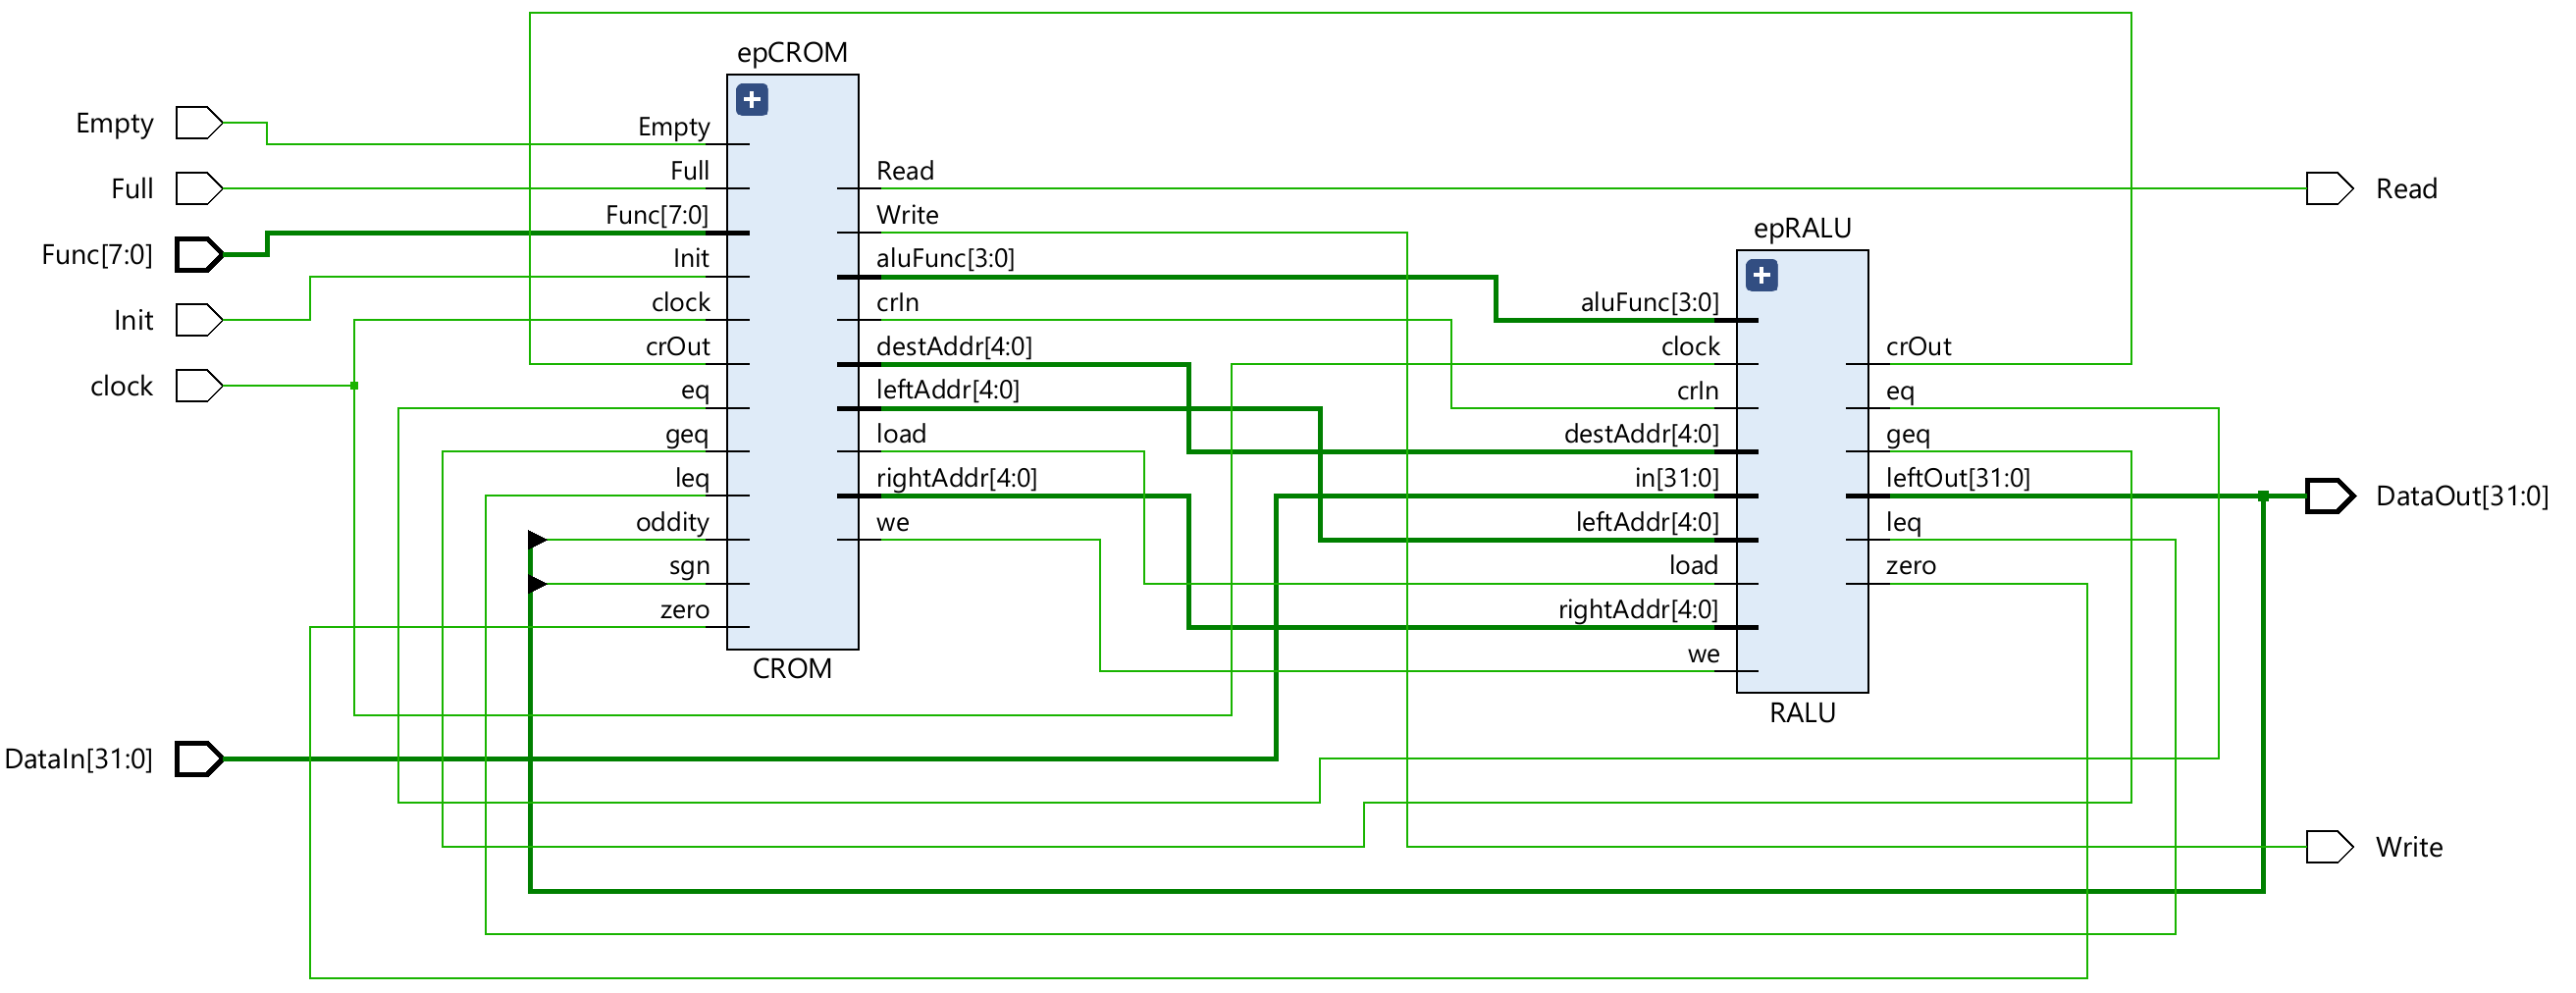
\includegraphics[width=\textwidth]{Images/elementaryProcessor.png} 
    \caption{Top level of the elementary processor generated in Vivado environment}
    \label{fig:elementaryProcessor}
\end{figure}

The simple functional automaton is a RALU, defined in Listing \ref{lst:elementaryProcessor}, unit with few additional simple circuits used to evaluate four flags besides the {\tt crOut} flag provided by the ALU output. They are evaluated on the two outputs of the register file, {\tt leftOut} and {\tt rightOut}, as follows: 

{\em 
\includeverilogcode[caption={RALU of Elementary Processor (EP).  File: 2\_RALU.sv  (SystemVerilog)}, 
                    label={lst:elementaryProcessor}, 
                    firstline=1, 
                    firstnumber=1, 
                    lastline=100]
                    {\verilogSourceDir/A11_RALU.sv}
}

\begin{itemize}
    \item {\tt eq}: equal,  {\tt leftOut == rightOut}
    \item {\tt leq}: less than or equal, {\tt leftOut <= rightOut}
    \item {\tt geq}: greater than or equal, {\tt leftOut >= rightOut}
    \item {\tt zero}: equal with zero, {\tt leftOut == 0}
\end{itemize}
To these five flags two are added by directly selected them from the {\tt leftOut} output of the register file:
\begin{itemize}
    \item {\tt sgn}: indicates the number selected by {\tt L(v)} is negative
    \item {\tt oddity}: indicates the number selected by {\tt L(v)} is odd
\end{itemize}

The complex, control automaton CROM is described in Listing \ref{lst:CROM}, while de resulting structure is represented in Figure \ref{fig:epCROM} as it is generated by the Vivado tool. The complex part of the subsystem is concentrated in the content of the RAM combinational circuit. The rest of the CROM unit contains only simple circuits register, increment circuit and multiplexers.

\begin{figure}[H]
    \centering
    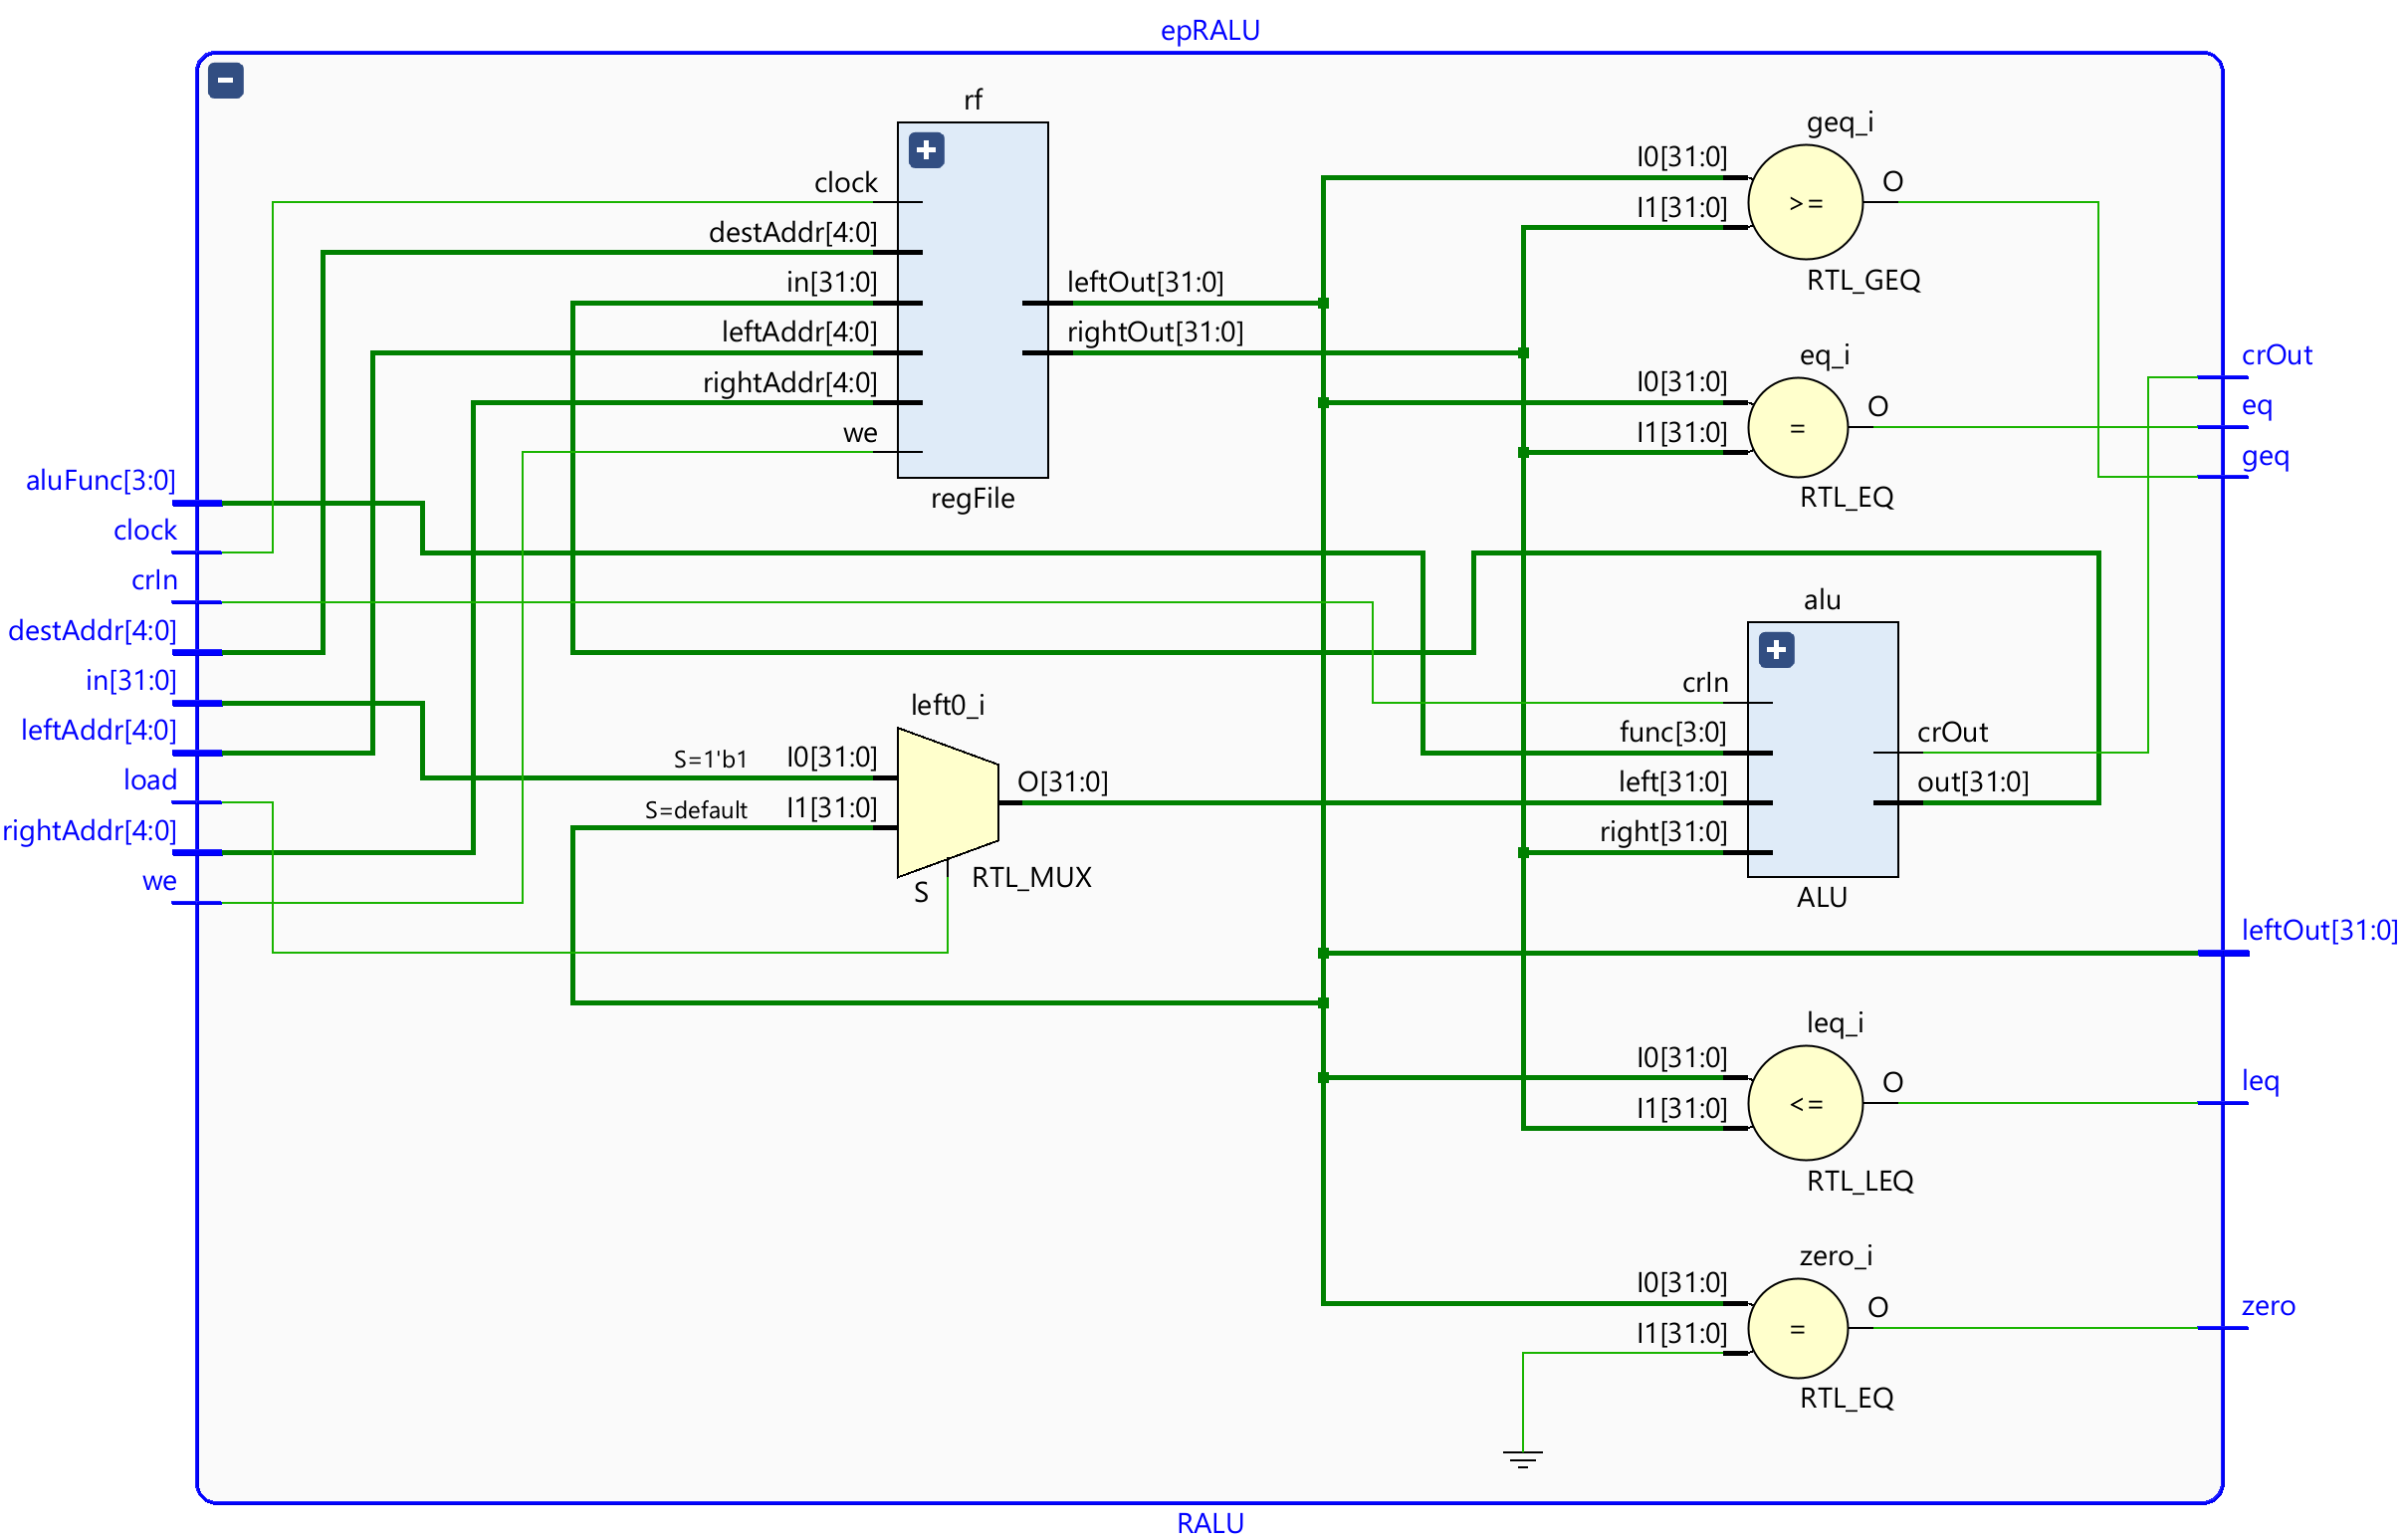
\includegraphics[width=\textwidth]{Images/peRALU.png} 
    \caption{epRALU.}
    \label{fig:peRALU}
\end{figure}

To the flags provided by the RALU unit there are added two flags received from the external systems:
\begin{itemize}
    \item {\tt Empty}: the data source applied to the input {\tt DataIn} is empty, i.e., does not provide a valid data input for PE
    \item {\tt Full}: the data receiver is full, i.e., it is unable to take the data provided on {\tt DataOut} output of PE.
\end{itemize}

{\em 
\includeverilogcode[caption={CROM of Elementary Processor (EP).  File: 2\_CROM.sv  (SystemVerilog)}, 
                    label={lst:CROM}, 
                    firstline=1, 
                    firstnumber=1, 
                    lastline=100]
                    {\verilogSourceDir/A11_CROM.sv}
}

\begin{figure}[H]
    \centering
    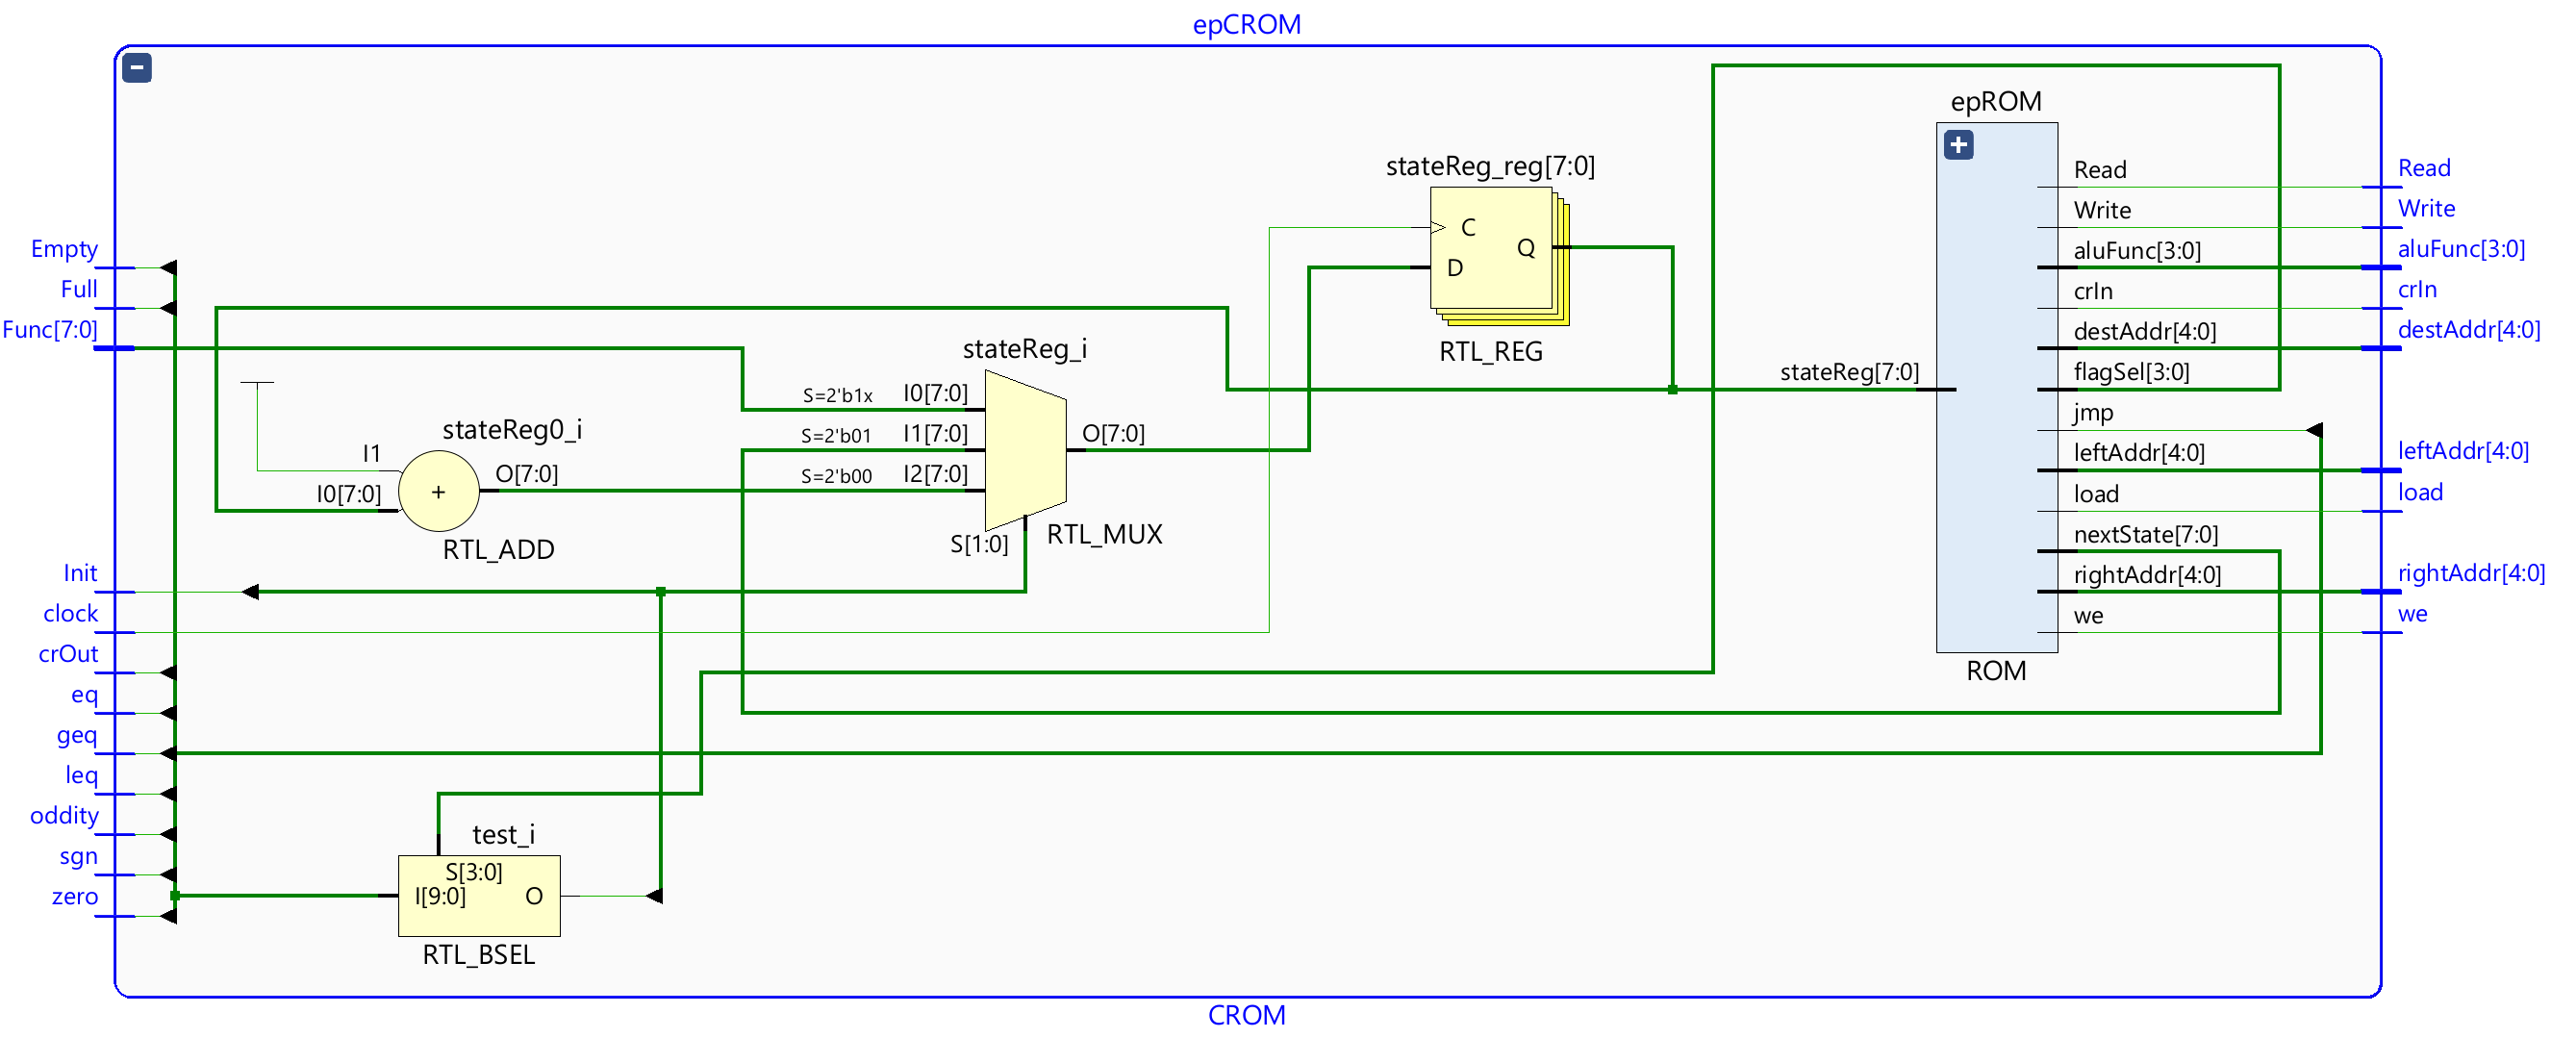
\includegraphics[width=\textwidth]{Images/epCROM.png} 
    \caption{epCROM.}
    \label{fig:epCROM}
\end{figure}

The third level of the design has two modules in RALU (register file and ALU) and one in CROM (the ROM circuit).

\begin{figure}[H]
    \centering
    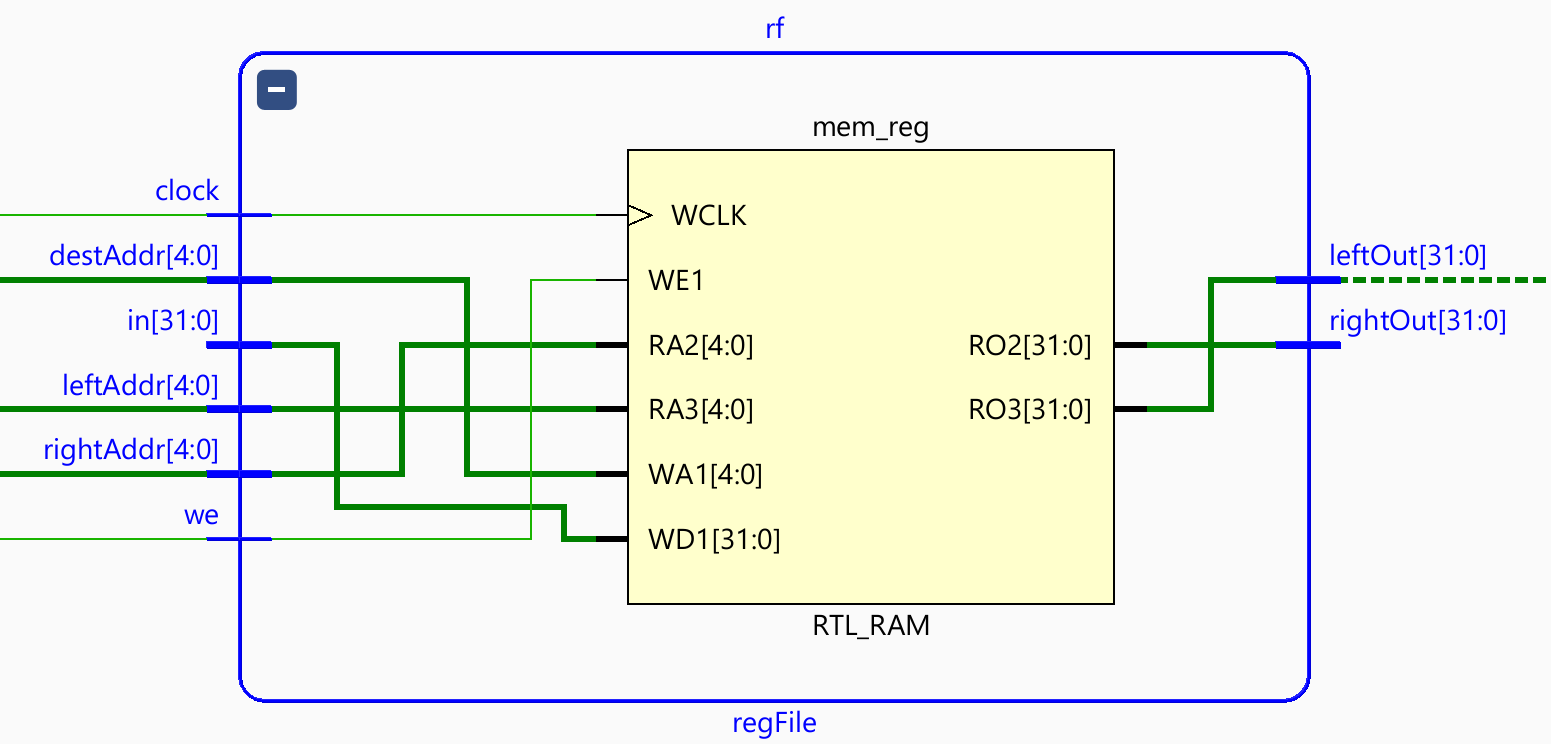
\includegraphics[width=\textwidth]{Images/epRegFile.png} 
    \caption{Register file.}
    \label{fig:epRegFile}
\end{figure}

In Listing \ref{lst:regFile} the structure and function of the register file is designed, while the resulting schemaatic is presented in Figure \ref{fig:epRegFile}. The register file is a synchronous memory for writing and asynchronous for reading.

{\em 
\includeverilogcode[caption={Register file.  File: 3\_regFile.sv  (SystemVerilog)}, 
                    label={lst:regFile}, 
                    firstline=1, 
                    firstnumber=1, 
                    lastline=100]
                    {\verilogSourceDir/A11_regFile.sv}
}

\begin{figure}[H]
    \centering
    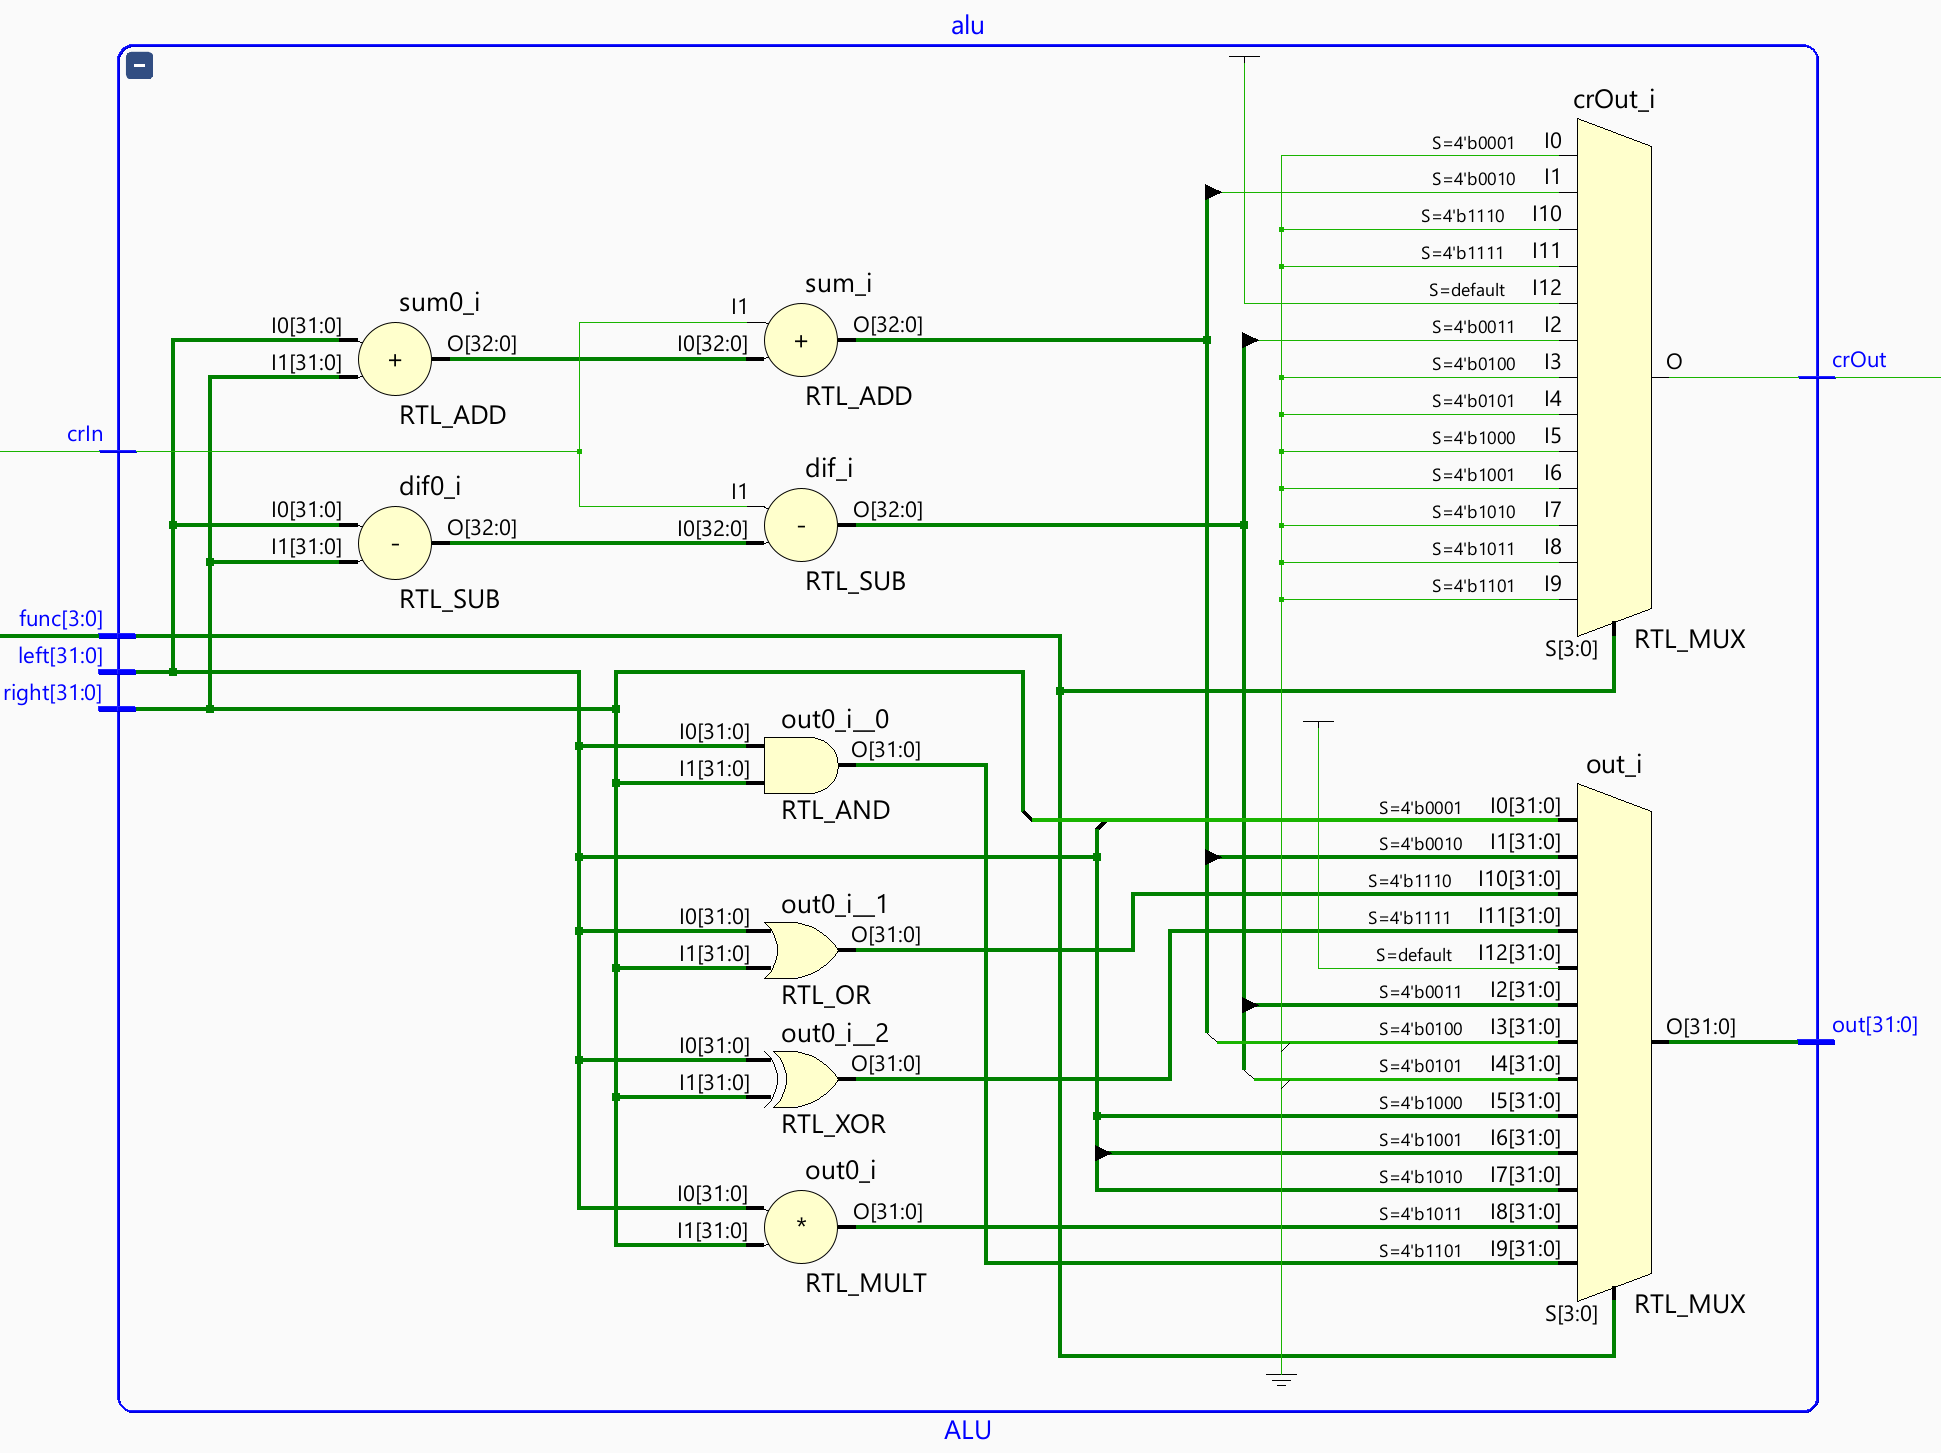
\includegraphics[width=\textwidth]{Images/epALU.png} 
    \caption{ALU.}
    \label{fig:epALU}
\end{figure}

In Listing \ref{lst:ALU} and Figure \ref{fig:epALU} the ALU used by the EP is described according to the {\tt 0\_define.vh} file (see Listing \ref{lst:define}).

{\em 
\includeverilogcode[caption={Define file for EP.  File: 0\_define.vh  (SystemVerilog)}, 
                    label={lst:define}, 
                    firstline=1, 
                    firstnumber=1, 
                    lastline=100]
                    {\verilogSourceDir/A11_define.vh}
}

{\em 
\includeverilogcode[caption={ALU.  File: 3\_ALU.sv  (SystemVerilog)}, 
                    label={lst:ALU}, 
                    firstline=1, 
                    firstnumber=1, 
                    lastline=100]
                    {\verilogSourceDir/A11_ALU.sv}
}

In Listing \ref{lst:ROM} and Figure \ref{fig:epROM} the ROM used by the CROM unit is structurally described. Its content is generated by {\tt \_microCodeGeneerator.sv} (see next subsection).

\begin{figure}[H]
    \centering
    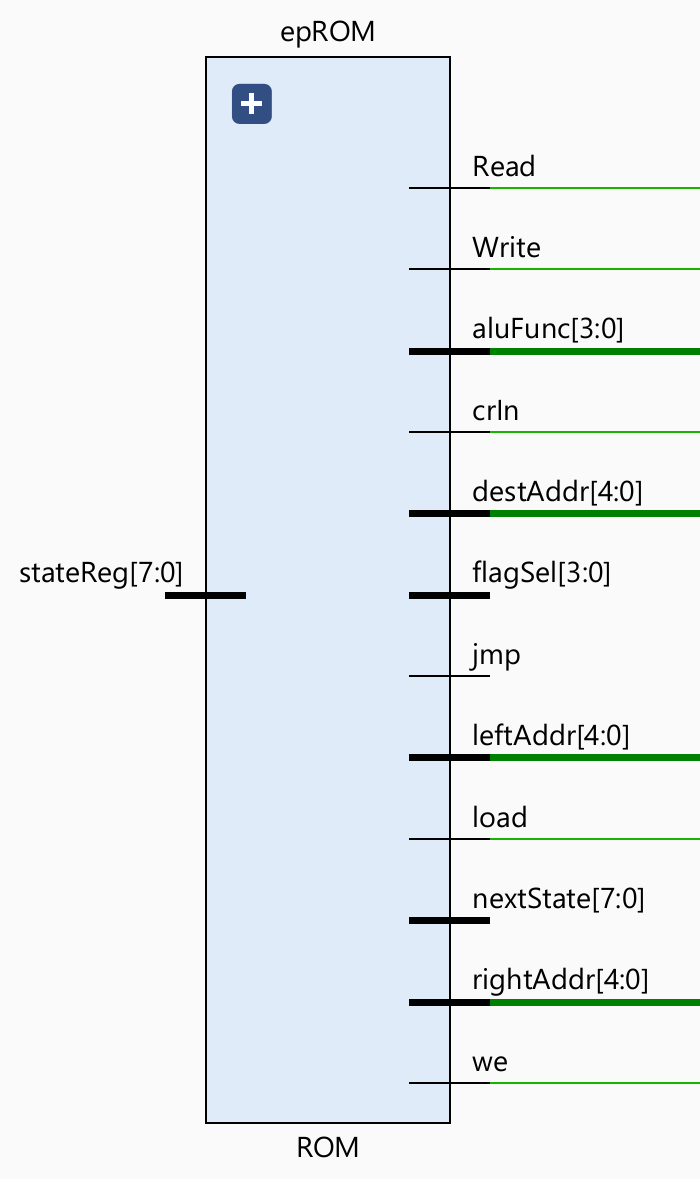
\includegraphics[width=6cm]{Images/epROM.png} 
    \caption{ROM.}
    \label{fig:epROM}
\end{figure}

{\em 
\includeverilogcode[caption={epROM.  File: 3\_ROM.sv  (SystemVerilog)}, 
                    label={lst:ROM}, 
                    firstline=1, 
                    firstnumber=1, 
                    lastline=100]
                    {\verilogSourceDir/A11_ROM.sv}
}


$\diamond$
\end{exemplu}

\subsection{Elementary Processor Micro-Programming}

Micro-programming an EP means to establish the content of CROM's ROM. We must follow the next steps:
\begin{enumerate}
    \item define the fields of the output word of ROM
    \item define the meaning designate by each field
    \item design the program which generate the binary form of each word (line) in ROM
    \item write the micro-programs associated for each function
\end{enumerate}

\subsubsection{Micro-Program's Fields}

A micro-instruction is organized in fields, according to the command issued by the CROM unit. In Example \ref{eProc}, the micro-program uses micro-instructions with the following 12 fields:
\begin{description}
    \item[{\tt nextState[7:0]}]: represents the value of the next state when it is not determined by increment; is is specified in assembly language through the label associated to the targeted line, and the micro-code generator takes care about the actual binary value inserted in the micro-instruction
    \item[{\tt jmp}]: unconditioned jump to {\tt nextState} specified by label; it acts in micro-instruction with the following mnemonic:
        \begin{description}
            \item[{\bf  JMP(<label>)}]: where {\tt <label>} is expressed by a number
        \end{description}
    \item[{\tt flagSel[3:0]}]: selects the flag according to which the jump is made to  {\tt nextState}; it acts in micro-instruction with the followings mnemonics:
    \begin{description}
        \item[{\bf CRJMP(<label>)}]: jump, if carry, to {\tt <label>} which is expressed by a number
        \item[{\bf ODDJMP(<label>)}]: jump, if left operand is an odd number, to {\tt <label>} which is expressed by a number
        \item[{\bf SGNJMP(<label>)}]: jump, if left operand is a negative numbe,r  to {\tt <label>} which is expressed by a number
        \item[{\bf ZJMP(<label>)}]: jump, if left operand is zero,  to {\tt <label>} which is expressed by a number
        \item[{\bf LEQJMP(<label>)}]: jump, if left operand is less or equal than right operand,  to {\tt <label>} which is expressed by a number
        \item[{\bf GEQJMP(<label>)}]: jump, if left operand is greater or equal than right operand,  to {\tt <label>} which is expressed by a number
        \item[{\bf EQJMP(<label>)}]: jump, if left operand is  equal with right operand,  to {\tt <label>} which is expressed by a number
        \item[{\bf EMPTYJMP(<label>)}]: jump if the sender system is empty (has nothing to send), where {\tt <label>} is expressed by a number
        \item[{\bf FULLJMP(<label>)}]: jump is the receiver is full (unable to receive), where {\tt <label>} is expressed by a number
    \end{description}
    \item[{\tt leftAddr[4:0]}]: address to select the left operand for ALU from register file; it acts in micro-instruction with the following mnemonic:
        \begin{description}
            \item[{\bf L(<address>)}]: where {\tt <address>} is expressed by a number
        \end{description}
    \item[{\tt rightAddr[4:0]}]: address to select the right operand for ALU from register file; it acts in micro-instruction with the following mnemonic:
        \begin{description}
            \item[{\bf R(<address>)}]: where {\tt <address>} is expressed by a number
        \end{description}
    \item[{\tt crIn}]: carry input applied to ALU; it acts in micro-instruction with the following mnemonic:
        \begin{description}
            \item[{\bf CR}]
        \end{description}
    \item[{\tt destAddr[4:0]}]: address to select the destination of the result computed by ALU; it acts in micro-instruction with the following mnemonic:
        \begin{description}
            \item[{\bf D(<address>)}]: where {\tt <address>} is expressed by a number
        \end{description}
    \item[{\tt load}]: selects as left operand DataIn; it acts in micro-instruction with the following mnemonic:
        \begin{description}
            \item[{\bf LOAD}]
        \end{description}
    \item[{\tt we}]: write enable applied to the register file; it acts in micro-instruction with the following mnemonic:
        \begin{description}
            \item[{\bf WB}]:write back
        \end{description}
    \item[{\tt aluFunc[3:0]}]: the arithmetic or logic function selected to be performed by ALU on the operands fetched form the register file; it acts in micro-instruction with the followings mnemonics:
        \begin{description}
            \item[{\bf BIGVAL}]: {\tt D(X) <= \{L(Y)[15:0], R(Z)[15:0]\}}, where $X,Y,Z \in [0,32)$
        \end{description}
        \begin{description}
            \item[{\bf ADD}]: {\tt D(X) <= L(Y) + R(Z)}, where $X,Y,Z \in [0,32)$
        \end{description}
        \begin{description}
            \item[{\bf SUB}]: {\tt D(X) <= L(Y) - R(Z)}, where $X,Y,Z \in [0,32)$
        \end{description}
        \begin{description}
            \item[{\bf ADDCR}]: {\tt D(X) <= (L(Y) + R(Z))[23]}, where $X,Y,Z \in [0,32)$
        \end{description}
        \begin{description}
            \item[{\bf SUBCR}]: {\tt D(X) <= (L(Y) - R(Z))[23]}, where $X,Y,Z \in [0,32)$
        \end{description}
        \begin{description}
            \item[{\bf RSH}]: {\tt D(X) <= \{1'b0, L(Y)[31:1]\}}, where $X,Y \in [0,32)$
        \end{description}
        \begin{description}
            \item[{\bf ASH}]: {\tt D(X) <= \{L(Y)[31], L(Y)[31:1]\}}, where $X,Y \in [0,32)$
        \end{description}
        \begin{description}
            \item[{\bf MOVE}]: {\tt D(X) <= L(Y)}
        \end{description}
        \begin{description}
            \item[{\bf MULT}]: {\tt D(X) <= L(Y) * R(Z)}, where $X,Y,Z \in [0,32)$
        \end{description}
        \begin{description}
            \item[{\bf AND}]: {\tt D(X) <= L(Y) \& R(Z)}, where $X,Y,Z \in [0,32)$
        \end{description}
        \begin{description}
            \item[{\bf OR}]: {\tt D(X) <= L(Y) | R(Z)}, where $X,Y,Z \in [0,32)$
        \end{description}
        \begin{description}
            \item[{\bf XOR}]: {\tt D(X) <= L(Y) $\oplus$ R(Z)}, where $X,Y,Z \in [0,32)$
        \end{description}
    \item[{\tt Read}]: read DataIn; it acts in micro-instruction with the following mnemonic:
        \begin{description}
            \item[{\bf GET}]: {\tt D(X) <= DataIn}
        \end{description}
    \item[{\tt Write}]: write DataOut; it acts in micro-instruction with the following mnemonic:
        \begin{description}
            \item[{\bf SEND}]: DataOut = L(Y), where $Y \in [0,32)$
        \end{description}
\end{description}

\subsubsection{Writing a micro-program}

A line of micro-code contains 37 bits. Each line is "stored" in a single location of the ROM in CROM. We used quotation marks because ROM is not a memory and its content is not stored, it is imprinted using a technological procedure. 

The micro-instruction is organized in fields as follows:
{\small
\begin{verbatim}
{jmp,nextState,flagSel,leftAddr,rightAddr,crIn,destAddr,load,we,aluFunc,read,write}
\end{verbatim}
}
Each line in a micro-program must by specified only by the fields with active forms. All the other fields will remain specified by zeroes. For example, the micro-instruction which moves the content of a register from the register file in other register, must specify, in any order, only the values for the fields {\tt destAddr, leftAddr, aluFunc,} and {\tt we}. All the other fields will be set to the default value which is zero.

\begin{exemplu}\label{mcex}
Let be a micro-program initialized by loading in registers three values received from the data input. Then operate on the received data running a loop {\tt rf[6]+1} times starting at the label {\tt LB(0)} and ending in halt at the label {\tt LB(55)}. The micro-program considers that the input signals {\tt Empty} and {\tt Full} are inactive (the sender sends data and the receiver accepts data).
{\em 
\includeverilogcode[caption={Example of micro-program.  File: 0\_microProgram.sv  (SystemVerilog)}, 
                    label={lst:microProgram}, 
                    firstline=1, 
                    firstnumber=1, 
                    lastline=200]
                    {\verilogSourceDir/A11_microProgram.sv}
}

Each line ends with {\tt LL}, the command used by the micro-code generator to {\bf l}oads the {\bf l}ine in ROM. This command allows avoiding to specifiy for each line all the fields.

$\diamond$
\end{exemplu}


\subsubsection{Micro-Code Generator}

The simulator will be described in \ref{elProcSim} the following code is included. It will receive the file {\tt 0\_microProgram.sv} to be translated into binary form.

\includeverilogcode[caption={Micro-code generator.  File: 0\_microCodeGenerator.sv  (SystemVerilog)}, 
                    label={lst:microCodeGenerator}, 
                    firstline=1, 
                    firstnumber=1, 
                    lastline=200]
                    {\verilogSourceDir/A11_microCodeGenerator.sv}



\begin{exemplu}
The micro-program from Example \ref{mcex} is translated in the following binary form using {\tt  0\_microCodeGenerator.sv} in the simulation module described in \ref{elProcSim}.

\begin{verbatim}
epROM[0]     = 0000000000000000000000000000011101000
epROM[1]     = 0000000000000000000000000010111101000
epROM[2]     = 0000000000000000000000000011011101000
epROM[3]     = 0000000000000000000000000000101001000
epROM[4]     = 0000000000000000010000100001001001000
epROM[5]     = 0000000000000000100001000001101001000
epROM[6]     = 0000000000000000110000000000001101000
epROM[7]     = 0000010010100001100010100011001001100
epROM[8]     = 1000000110000000000000000000000000000
epROM[9]     = 1000010010000000000000000000000000000
epROM[10]    = xxxxxxxxxxxxxxxxxxxxxxxxxxxxxxxxxxxxx
\end{verbatim}

$\diamond$
\end{exemplu}

\subsubsection{Elementary Processor Simulation}\label{elProcSim}

To test the operation of the elementary processor, we use the module in Listing \ref{lst:epTest} which generates the binary code of the micro-program and provides the external stimuli ({\tt clock, Inint, Func, DataIn, empty, Full}) for running the micro-program.

\includeverilogcode[caption={EP tester.  File: 0\_epTest.sv  (SystemVerilog)}, 
                    label={lst:epTest}, 
                    firstline=1, 
                    firstnumber=1, 
                    lastline=200]
                    {\verilogSourceDir/A11_epTest.sv}

\begin{exemplu}
The micro-program in Listing  \ref{lst:microProgram}  from Example \ref{mcex} works in conjunction with the stimulus generated by the simulation environment. Lines of code from 34 to 443 in Listing \ref{lst:epTest} provide the context for running the micro-program in Listing  \ref{lst:microProgram}. Results:
{\small
\begin{verbatim}
t=0  Func=0 Init=1 stateReg=x DataOut=x    test=x RF=[x x x x x x x x x]
t=1  Func=0 Init=1 stateReg=0 DataOut=x    test=0 RF=[x x x x x x x x x]
t=2  Func=0 Init=0 stateReg=0 DataOut=x    test=0 RF=[x x x x x x x x x]
t=3  Func=0 Init=0 stateReg=1 DataOut=3    test=0 RF=[3 x x x x x x x x]
t=5  Func=0 Init=0 stateReg=2 DataOut=3    test=0 RF=[3 x x x x 1 x x x]
t=7  Func=0 Init=0 stateReg=3 DataOut=3    test=0 RF=[3 x x x x 1 2 x x]
t=9  Func=0 Init=0 stateReg=4 DataOut=6    test=0 RF=[3 6 x x x 1 2 x x]
t=11 Func=0 Init=0 stateReg=5 DataOut=12   test=0 RF=[3 6 12 x x 1 2 x x]
t=13 Func=0 Init=0 stateReg=6 DataOut=24   test=0 RF=[3 6 12 24 x 1 2 x x]
t=15 Func=0 Init=0 stateReg=7 DataOut=2    test=0 RF=[24 6 12 24 x 1 2 x x]
t=17 Func=0 Init=0 stateReg=8 DataOut=24   test=1 RF=[24 6 12 24 x 1 1 x x]
t=19 Func=0 Init=0 stateReg=3 DataOut=24   test=0 RF=[24 6 12 24 x 1 1 x x]
t=21 Func=0 Init=0 stateReg=4 DataOut=48   test=0 RF=[24 48 12 24 x 1 1 x x]
t=23 Func=0 Init=0 stateReg=5 DataOut=96   test=0 RF=[24 48 96 24 x 1 1 x x]
t=25 Func=0 Init=0 stateReg=6 DataOut=192  test=0 RF=[24 48 96 192 x 1 1 x x]
t=27 Func=0 Init=0 stateReg=7 DataOut=1    test=0 RF=[192 48 96 192 x 1 1 x x]
t=29 Func=0 Init=0 stateReg=8 DataOut=192  test=1 RF=[192 48 96 192 x 1 0 x x]
t=31 Func=0 Init=0 stateReg=3 DataOut=192  test=0 RF=[192 48 96 192 x 1 0 x x]
t=33 Func=0 Init=0 stateReg=4 DataOut=384  test=0 RF=[192 384 96 192 x 1 0 x x]
t=35 Func=0 Init=0 stateReg=5 DataOut=768  test=0 RF=[192 384 768 192 x 1 0 x x]
t=37 Func=0 Init=0 stateReg=6 DataOut=1536 test=0 RF=[192 384 768 1536 x 1 0 x x]
t=39 Func=0 Init=0 stateReg=7 DataOut=0    test=1 RF=[1536 384 768 1536 x 1 0 x x]
t=41 Func=0 Init=0 stateReg=9 DataOut=1536 test=1 RF=[1536 384 768 1536 x 1 -1 x x]
\end{verbatim}
}

$\diamond$
\end{exemplu}



\section{Processor}\label{toyRISCprocessor}

The elementary processor defined above is capable of executing a single function using the microprogram written in the ROM associated with the CROM. If we call this single function an instruction, then it would be interesting if we could extend the functionality of the elementary processor to that of a processor that can execute a sequence of instructions. Instead of "waiting" for the activation of the external signal {\tt Init}, the processor can manage to fetch from a memory, which is external to it, the next instruction every time the current one has been executed. Furthermore, a processor is equipped with the capability of fetching from an external memory the data that it decides to use, not only those made available by an external mechanism as in the case of the elementary processor.

The internal state of the processor is given by the Cartesian product represented by the contents of the register file. The evolution of the internal state of the processor, under the influence of the sequence of instructions it controls and the data it accesses in the external memory, as well as the effect of this evolution on the data in the external data memory, are controlled by the sequence of instructions designed to be stored in a memory external to the processor. Under these conditions, the operation of a processor is determined by its hardware structure and the software structure of the programs it runs. For this reason, the description of a processor involves the complementary processes of defining the organization and architecture.

\subsection{Architecture\index{architecture: the user's image of a processing engine; describes what it does} vs. Organization\index{organization: the structure of a processor; describes how the processor does what it does}}\label{archOrg}

{\small
 \hfill{
\begin{minipage}{8cm}
{\em Architecture: describes what the processor does.

Organization: describes how it does it.}
\end{minipage}
}}

\bigskip
In the beginning it was only the hardware and the software. At some point there was a need for an interface that would provide the software with a more friendly development environment. What it is? If in a suite of hardware implementations the set of instructions changes radically with each new version, then the programs written for previous versions are thrown into the trash every time a new hardware version is instantiated. This bad habit is cured with the design, at the beginning of the 1960s, of the IBM System/360\index{IBM System/360: first computer family with unified instruction set architecture}. At that moment it was decided that:
\begin{quote}
{\em ... to describe the
attributes of a system as seen by the programmer, i.e., the conceptual structure
and functional behavior, as distinct from the organization of the data flow and
controls, the logical design, and the physical implementation.} \citep{Amdahl64}\index{Amdahl, Gene: computer architect and pioneer of IBM System/360}
\end{quote}
And so the {\em Hardware -- Software} duet turned into the {\bf {\em Hardware -- Architecture -- Software}} triplet. Architecture being the short form for Instruction Set Architecture, ISA\index{ISA|see{instruction set architecture}}\index{instruction set architecture (ISA): boundary between hardware and software}.
\begin{table}[H]
  \begin{center}
    \caption{Architecture vs. Organization.}
    \label{avso}
    {\small
    \begin{tabular}{|p{6cm}|p{6cm}|}
      \hline
     {\bf Architecture}                 & {\bf Organization}                                \\ \hline \hline
     describes what the processor does   & describes how it does it                          \\ \hline
     deals with the functional behavior & deals with a structural relationship              \\ \hline
     architecture is fixed first        & organization is decided after     \\ \hline
     comprises instruction sets, registers, data types, and addressing modes & consists of  multiplexers, adders, multipliers, peripherals, memories, ...\\ \hline
     the software developer is aware of it & it escapes the software programmer’s detection\\ \hline
    \end{tabular}
    }
  \end{center}
\end{table}


There are several ways to close the third loop over a generic 2-OS represented by an automaton in order to obtain the generic structure o a {\bf processor}. On the closed loop over an automaton we can connect a 0-OS (a combinational circuit), a 1-OS (a memory), or a 2-OS (an automaton). The last version is the most significant (see Figure \ref{fig40}). It is the main subject of this chapter.

The two machines that configure a processor have distinct functions:

\placedrawing[H]{figures/05_01_generic_processor.lp}{Generic processor: an engine capable of controlling the retrieval of data and instructions from the external memory source.}{fig40}

\begin{itemize}
    \item functional automaton that performs data processing functions; it is a simple automaton
    \item control automaton that ensures the sequential operation of the processor implemented in two possible versions:
        \begin{itemize}
            \item  a complex controller of the type presented in \ref{contrAut}, when, in addition to fetching the instruction from the program memory, it is also necessary to break it down into a sequence of micro-instructions executed by the functional automaton
            \item  a simple controller of the counter type presented in \ref{progCounter}, when it is sufficient to bring the instruction from the program memory because the instruction is simple enough to be executed directly by the functional automaton
        \end{itemize}
\end{itemize}

The two types of control generate two types of processors: interpreting processor and executing processor.

\subsection{Interpreting Processor (CISC\index{CISC (Complex Instruction Set Computer): a computing system in which the instructions are interpreted by a sequence of microinstructions} processor)}

The first type of processor, the one that interprets the instruction by decomposing it into a sequence of microinstructions, is represented in Figure \ref{fig41}, where the control is performed with a complex automaton. An instruction can involve complex operations implemented sequentially through a series of micro-instructions sent by the controller to the functional automaton that can send back to the controller flags that can characterize the result of the application of each micro-instruction. For this reason, this processor version is called CISC (Complex Instruction Set Computer).

For each instruction the CISC processor must perform:
\begin{enumerate}
    \item instruction fetch
    \item instruction execute
    \item compute the address for the next instruction
\end{enumerate}

\placedrawing[H]{figures/05_02_interpreting_processor.lp}{Interpreting Processor}{fig41}

\hspace{-5mm}so that an instruction is executed in a variable number of at least several clock cycles.

\subsection{Executing Processor (RISC\index{RISC (Reduced Instruction Set Computer): a computing system in which the instructions are executed in constant time (usually one clock cycle)} processor)}

The second type of processor is designed in such a way that it executes each instruction in constant time, usually one clock cycle, but no more than two clock cycles. Because each instruction requires fetching it from memory, and some instructions also require writing or reading data from memory, it is necessary to structure the memory into two sub-memories, one for programs and another for data. This results in the structure in Figure \ref{fig42}, where the processor has two access paths to memory resources.
In this case, the control automaton can only take care of fetching the instructions from the program memory and the functional automaton will execute sufficiently simple instructions to require only one clock cycle to be operated.

How did you get to this way of designing a processor that executes only simple, executable instructions in one clock cycle? Around 1980, the following facts were evident:

\placedrawing[H]{figures/05_03_executing_processor.lp}{Executing Processor}{fig42}

\begin{itemize}
    \item the frequency with which the instructions of a CISC processor appeared in the programs was very variable: a small number of instructions had a very high frequency of use, and the majority were used with low frequencies

    \item if the instructions were listed in descending order of frequency of use, then a line could be drawn in this list delimiting a set of frequently used instructions that also had the quality of being able to implement the instructions below the line through a suitable sequencing of them

    \item the pleasant surprise was that only simple functions were found above the line

    \item thus, for frequent operations, the effector structure could be imagined to work quickly, and for the less frequent ones, the possibility of their performance is ensured
\end{itemize}
Thus, a RISC processor executes instead of interpreting. Programs represent sequences of simple instructions, which are executed in parallel with the control of their evolution. Indeed, the functional automaton operates on the data while the control automaton calculates the address from which the next instruction will be read.
Both types of operations fall into the category of simple ones, the fact that it allows us to consider a RISC processor as simple to distinguish it from a CISC one which is complex due to the control automaton.

\bigskip

Since the functionality of a processor is exercised in the context of its use as a unit that runs a program stored in an external memory, we prefer to analyze in detail the functioning of a processor as part of a computing system. We will prefer to analyze in detail a RISC processor, an analysis that we will do in the context of a 5th order digital system (see Chapter \ref{lect6a}).


\section{Problems}

\subsection{Counter-Expanded Automata}

\begin{problem}
Design and simulate FA defined in Example \ref{ceaEx} by the graph represented in Figure \ref{ceaExGraph}.

$\diamond$
\end{problem}

\begin{problem}
Consider the language $L = \{a^nb^3c^4 \;| \; n>0\}$. Design the CEA which recognize this language. It is required:
\begin{enumerate}
    \item defining the graph which describes the associated finite automaton
    \item describing in System Verilog the CEA 
    \item verification of the design by simulation.
\end{enumerate}

$\diamond$
\end{problem}

\begin{problem}\label{pda}
Reconsider the structure defined in Example \ref{ceaEx} by substituting the up-down counter with the LIFO memory described in \ref{lb:lifo}. The initial top of stack must be a special symbol, $Z_0$. The resulting structure is called in literature: {\em push-down automaton}.

$\diamond$
\end{problem}


\begin{problem}
Use the push-down automaton designed in Problem \ref{pda} to solve the problem of recognizing $L = \{a^nc^4 \;| \; n>0\}$.

$\diamond$
\end{problem}

\subsection{Elementary Processor}

\begin{problem}
In Example \ref{mcex} the is considered {\tt Empty = 0} and {\tt Full = 0} during the test. Rewrite the micro-program considering that the two signals can take both the value 0 and the value 1 during the test. Test the correct functioning of the program using the Vivado environment and the simulator available on GitHub.

$\diamond$
\end{problem}

\begin{problem}
Modify the design of the elementary processor PE so that the new version, PE1, has the ability to generate, using CROM resources, constants that can be loaded into the register file.

$\diamond$
\end{problem}

\begin{problem}
Using PE1, design a  discrete-time FIR filter of order N, for $N=16$ taps, which receives a sting of integers, $x[i]$, and issues another string of integers, $y[j]$ according to the following expression:
$$y[n] = \sum_0^N b_ix[n-i]$$
The taps are generated in the definition of CROM.

$\diamond$
\end{problem}

\begin{problem}
Replace in PE the RALU with the SALU defined in Problem \ref{lb:salu}. Describe in System Verilog and simulate he resulting Stack Elementary Processor, SEP. Comment on advantages and disadvantages on SEP compared to the PE/PE1 version.

$\diamond$
\end{problem}


%################
\part{COMPUTING}
%################
\chapter{Computers\index{computers:  fourth order digital systems (4-OS) with the fourth loop  closed over a 3-OS}: Four-Loop, Fourth-Order Systems (4-OS)\index{4-OS: fourth order system -- interpreting computer}}\label{lect6}\label{ch:von_neumann_4-OS}
\localtoc


At the level of the fourth loop, we are at a {\em turning point} where the physical structure of the circuits will meet the informational structure of the programs. The functionality will be determined starting from this point by the circuit-information combination. The interface between structural and informational aspects is provided by the concept of {\bf {\em architecture}} borrowed from the field of construction.









After the first part of this textbook described the symbolic structures involved in computing, and the second part described the physical structures that can be used to implement computing systems, the time has come to involve the unifying entity represented by {\bf {\em information}}. Indeed, information is the one that takes control once the serendipitous meeting between representations, physical structures, and an acting symbolic structure occurs. The symbolic structure we are referring to is the information that manifests itself in the form of computer programs. Computing systems represent the synthesis between the physical structure of circuits and the symbolic structure of programs. This was made possible by a conceptual clarification -- the emergence of mathematical models of computation -- and a technological evolution -- the structuring of digital systems by increasing their autonomy through the impact of included loops.


\section{The mathematical model of the Turing Machine}

In current language we use the term computation without a rigorous definition. When we have to substantiate the concept of computability and computation, rigor is absolutely necessary. We will continue with not only a historical but also a theoretical introduction to the concept of computation in the sense in which it is conceived in computational science.

\subsection{The Decision Problem}

Despite appearances, computers are not numerical instruments but logical structures that have their theoretical origin in solving decision-making problems. To the question: {\em where and when does the history of computers begin?}, the answer, however strange it may seem, is: {\em somewhere on the island of Crete about two and a half millennia ago}. Indeed, Epimenides of Knossos\index{Epimenides of Knossos (7th or 6th century BC): a semi-mythical Greek seer credited for the liar paradox} (the capital of the island of Crete), a semi-mythical Greek seer from the 7th or 6th century BC, caught himself saying that {\em "all Cretans are liars"}. Surprised, because in the next second he could not {\bf decide} whether the assertion he had just made was true or false. Thus was born, if the story is true, a problem that occupied the minds of seekers for millennia until it was rigorously reformulated by David Hilbert (1862–-1943)\index{Hilbert, David (1862–-1943): German mathematician and philosopher credited for rigorously stating the decision problem} and definitively settled by Kurt G\" odel (1906--1978)\index{G\" odel, Kurt (1906--1978): Austrian logician, mathematician and philosopher credited for the incompleteness of formal theories}.

Hilbert's address of 1900 to the International Congress of Mathematicians in Paris is perhaps the most influential speech ever given about mathematics \cite{Hilbert1900}. In it, Hilbert outlined 23 major mathematical problems to be studied in the coming century. One of them, the 10th, raises the issue of decision in a particular case. But, in a definitive form the problem is exposed in the book that David Hilbert writes together with Wilhelm Ackermann \cite{Hilbert1928}. This book included a clear statement of the {\em Entscheidungsproblem}\index{Entscheidungsproblem: Hilbert's decision problem in formal logic} (decision problem): 
\begin{quote}
    {\em is there an algorithm that takes a statement formulated in a formal system and answers with "yes" or "no" whether the statement is true or false in the given system?}
\end{quote}
The first answer comes in 1931 from the logician  Kurt Gödel: 
\begin{quote}
{\bf {\em in a formal system one can correctly construct true structures whose truth cannot be proven or disproved}} \cite{Goedel1931} \cite{Goedel31}.
\end{quote}

Gödel's spectacular result triggered within five years four mathematicians Alonzo Church\index{Church, Alonzo: logician who formulated lambda calculus and Church-Turing thesis}\index{Church-Turing thesis: conjecture that all effective computation is computable by Turing machine} \cite{Church36}, Stephen Kleene \cite{Kleene36}, Emil Post \cite{Post36}, and Alan Turing \cite{Turing36, Turing1937} (listed alphabetically) to independently provide works that founded computer science. We focus in this chapter on Turing's work.

\subsection{Turing Machine}

In his paper, about "computable numbers" and {\em Entscheidungsproblem}, Alan Turing\index{Turing, Alan (1912-1954): English mathematician, computer scientist, logician, cryptanalyst, philosopher and theoretical biologist credited for Turing Machine, a mathematical model for computation} describes in words what he called a {\em computing machine}. We call it now Turing Machine (TM) and we describe it as a structure with three components (see Figure \ref{tm}a):
\begin{itemize}
    \item an infinite {\bf tape}\footnote{It is most likely that Turing was inspired by the telegraph communication systems of the 1930s that used a paper tape to receive messages.}  on/from which symbols belonging to a finite set of symbols -- the machine's alphabet -- can be write or read using
    \item an accessing write/read {\bf head} which can move in each clock cycle one position to left or right under the control of
    \item a {\bf finite automaton} (FA) whose state is updated in each clock cycle according to its state and the symbol accessed from the tape.
\end{itemize}
The translation into a representation containing digital components is shown in Figure \ref{tm}b, where the infinite tape is substituted by an infinite RAM addressed by an up-down counter. 

\placedrawing[H]{figures/12_02_turingMachine.lp}{Turing Machine. {\bf a.} Original description: Tape \& Head \& FA. {\bf b.} Digital representation: Memory \& upDownConter \& FA.}{tm}

TM is a mathematical concept because of its unlimited tape. This "infinity" is due to the fact that at the beginning of the computation the size of the space required on the tape is not known. This ignorance is dealt with by the mathematician Turing with the convenient concept of infinity. But it is beyond any doubt that any real useful computation must be done in a finite number of cycles, so we never traverse an infinite memory.


\subsection{Theoretical Foundations of Number Representations in Turing's Work}

Alan Turing’s 1937 paper, “On Computable Numbers, with an Application to the Entscheidungsproblem,” primarily focuses on the concept of computability rather than explicit number representations used in modern computer systems. However, the theoretical groundwork Turing established lays the foundation for how numbers (and more broadly, data) can be represented and manipulated by machines. Here are the key theoretical points from Turing's paper that relate to number representations:

\subsubsection{Definition of Computable Numbers}

Turing defines a \textbf{computable number} as a real number that can be calculated to any desired precision by a mechanical process. Formally, a number \( x \) is \textbf{computable} if there exists an algorithm (what Turing termed a \textbf{computing machine}, now known as a Turing Machine) that, given an integer \( n \), can compute the \( n \)-th digit of \( x \) in a finite number of steps.

In modern terms:
\[
x = \sum_{i=1}^{\infty} d_i \cdot b^{-i}
\]
where \( d_i \) are digits (either binary, decimal, or other bases) and \( b \) is the base. Turing’s framework implies that, to represent \( x \) as computable, there must be a recursive procedure for determining \( d_i \) for all \( i \).

\subsection{Representation of Numbers Using Symbols and States}

Turing’s model introduced the concept of a machine that reads, writes, and moves over a tape. The tape holds symbols from a finite alphabet, which can be used to represent numbers in various bases, including binary. Each number can thus be represented by a sequence of symbols on the tape, with the \textbf{state of the machine} directing operations on these symbols.

Formally:
\begin{itemize}
    \item Let \( \Sigma = \{0, 1\} \) represent the binary alphabet.
    \item A \textbf{string} \( w \in \Sigma^* \) on the tape can represent a binary number, where the position and value of each symbol denote its magnitude.
\end{itemize}

\subsubsection{Finite State Automaton for Number Manipulation}

Turing proposed that any computable function, including arithmetic operations on numbers, could be executed by a sequence using a finite set of states. Each pair 
\begin{verbatim} 
         {state, symbol_currently_accessed_on_tape} 
\end{verbatim} 
directs the machine to either:
1. Write or erase a symbol, 
2. Move left or right along the tape.
3. Transition to another state.

This \textbf{finite state control} is the precursor to binary arithmetic and logical operations on numbers. It implies that any number representation (binary, decimal, or otherwise) can be manipulated using a finite sequence of state transitions based on the machine's rules.

\begin{definition}
Formally, for a Turing Machine\index{TM (Turing Machine)} \( M(T) \), we have:
\[
M = (Q, \Sigma, \delta, q_0, F)
\]
where:
\begin{itemize}
    \item \( Q \) is a finite set of states,
    \item \( \Sigma \) is the finite tape alphabet,
    \item \( \delta: Q \times \Sigma \to Q \times \Sigma \times \{L, R, -\} \) is the transition function, where $L$ and $R$ moves the access head one position to left or right,
    \item \( q_0 \in Q \) is the initial state,
    \item \( F \subseteq Q \) is the set of final (or halting) states.
\end{itemize}
and a tape $T$ whose content is initially, in the state $q_0$,  accessed with the read/write head positioned on the first symbol.

$\diamond$
\end{definition}
This structure allows \( M(T) \) to handle number representations in binary or any base by processing symbol strings according to their state rules in a finite number of cycles. In other words, for any function $F: X \rightarrow Y$ there exists a TM whose finite automaton, starting from the initial state $q_0$ and having on the tape $x \in X$, reaches a final state, $q_f$, and generates on the tape, after a finite number of steps, $y \in Y$ if $F(x) = y$.

{\bf Important note}: for each computable sequence another TM is needed.

\subsubsection{Concept of Universal Representation}

In Turing's words:
\begin{quote}
{\em It is possible to invent a single machine which can be used to compute
any computable sequence. If this machine $\cal U$ is supplied with a tape on
the beginning of which is written the S.D of some computing machine $\cal M$
then $\cal U$ will compute the same sequence as $\cal M$.} \cite{Turing36}
\end{quote}

Turing’s concept of a \textbf{Universal Turing Machine}\index{UTM (Universal Turing Machine)}, UTM, suggested that any computable number or function could be represented and processed by a single machine capable of interpreting encoded instructions for any specific computation. This idea led to the realization that numbers can be encoded as \textbf{data} or \textbf{instructions}, providing a basis for multiple forms of number representation and manipulation in modern computers.

If \( p \) is a program (or representation) for a number \( x \), then \( U(p) = x \), where \( U \) is a UTM capable of simulating \( p \). Given that a finite automaton has, by definition, a complex structure, theoretical research has carefully evaluated various versions for the FA associated with the UTM. We mention two limiting cases. One is that of the work of Claude Shannon who publishes a paper describing a UTM with an automaton having only 2 states \cite{Shannon56}. The consequence of this limitation is a combinational circuit on the loop of the 2-state finite automaton of very large size. Another occurs after 50 years. It is  a paper in which the finite automaton has zero states, that is, it is no longer necessary \cite{Stefan06Turing}. This establishes the possibility of simple processors, the RISC type, processors built only from simple recursively defined circuits.  

Formally: for any computation done by a TM $M(T)$ can be used the UTM $${\cal U}(<M,T>)$$ where the stream of symbols $M$ describes the automaton of the TM $M(T)$, while the stream of symbols $T$ is the tape of the same TM. In contemporary terms, $M$ is the program, while $T$ is data , both stored in the same memory.

\subsection{Summary of Key Theoretical Points in Turing's Paper}

\begin{enumerate}
    \item \textbf{Computable Numbers}: Defined as numbers that can be calculated to any precision using a finite, mechanical process.
    \item \textbf{Finite State Control}: Established that a finite set of states could operate on symbols to represent numbers in various bases.
    \item \textbf{Machine-Based Representation}: Showed that numbers could be represented as sequences of symbols on a tape, manipulated by a machine’s states and transitions.
    \item \textbf{Universal Representation}: Introduced the idea that numbers (or their representations) could be treated as data or instructions, leading to flexible encoding schemes for number manipulation.
\end{enumerate}

Turing’s formal model set the stage for understanding how numbers can be systematically represented, stored, and manipulated by computational systems, laying foundational principles that influence number representations in modern computing.

\section{von Neumann Abstract Model}\index{von Neumann architecture: computer architecture with shared memory for instructions and data}\index{von Neumann, John (1903--1957): mathematician and computer architecture pioneer}

TM is a mathematical model. The actual computing machines need an {\bf {\em intermediate model}}: an {\bf abstract} one, able to solve the problem of computation using real entities. In this "moment" comes the  serendipitous  meeting between math and tech, between UTM and digital circuits. In the abstract model proposed by the mathematician John von Neumann the finite automaton and the accessing head are integrated in what we call a processor which communicate with the memory which contains  programs and data (see Figure \ref{fig44}). 

%\section{von Neumann Computer Version: Four-Loop, Four-Order System ({\bf 4-OS})}

The two types of processors defined in the previous section were used to define two abstract computer models.

\smallskip

{\bf Historical note}: in the 1940s, the first electronic computers were made in two versions that generated two models for the subsequent evolution. Traditionally, but erroneously, these models are called {\em architectures}. The concept of architecture appeared in the 1960s. For this reason, we will call these concepts {\em abstract models} instead of architectures.

\smallskip


\placedrawing[H]{figures/05_04_von_neumann.lp}{The abstract model of computer proposed by  John von Neumann.}{fig44}

The interpretive processor is used in the definition of the {\em von Neumann abstract model}, in which the processor is loop connected to a single memory in which both programs and data are stored (see Figure \ref{fig44}). Thus, a 4-OS is obtained by connecting a 3-OS (Processor) with a 1-OS (Memory).


\section{System Organization}

The processor is the core of a computing system that contains also a memory subsystem and an input-output subsystem. The physical resources involved are tightly interleaved in various form of actual organization. The memory associated with the processor contains programs and data, while the input-output system has two main functions: expanding the memory capacity and ensuring the interaction of the system with the outside world.

\placedrawing[H]{figures/12_01_computing_components.lp}{The three-partite functionality of a computing system.}{pmio}

The way in which the tripartite functionality is distributed in a given system shows significant variations from one implementation to another. In the following, we will limit ourselves to a simple version, but not simpler than one that allows us to introduce the main concepts and problems. But, first we will show the serendipitous way in which the evolution of logic circuits meets a fundamental mathematical model for what can be rigorously defined as computation.

How looks the actual structure of a computing system? In Figure \ref{compSys} is exemplified a system where are emphasized two buses: the internal bus and the input-output bus. They are interconnected by two units: Bus Bridge and DMA (Direct Memory Access).

On Internal Bus are connected fast devices while on the Input-Output Bus are connected devices involving a lot of data transfer.

The memory hierarchy is distributed in the version represented in Figure \ref{compSys}  as follows:
\begin{enumerate}
    \item Register File in the processor, having a capacity of 32W $\div$ 1024W, accessed for reading or writing in a single clock cycle
    \item Cache memory, having a capacity of 1MB $\div$ 8MB
    \item Hard Disk connected through: Bus Bridge and DMA
\end{enumerate}

\placedrawing[H]{figures/06_08_computer_organization.lp}{The organization of a von Neumann version of a computing system.}{compSysN}

\section{Storage Systems: Primary and Secondary Memory}\label{sec:storage_systems}

In the fourth-order system (4-OS) interpretive abstract model (traditionally designated as the von Neumann abstract model \cite{vonNeumann1945}), the \textbf{Memory} ($\mathbf{M}$) represents a single, uniform, linear address space that stores both program instructions and numerical operands. As examined in the historical analysis of Section \ref{sec:first_draft_facts}, this stored-program concept emerged from the collaborative work at the Moore School of Electrical Engineering by J. Presper Eckert, John Mauchly, Arthur Burks, Herman Goldstine, and John von Neumann, grounded in Alan Turing's mathematical model of computation \cite{Turing36}. In this foundational abstract formulation, storage was conceived without microarchitectural hierarchy: the central processing unit (3-OS) interacted directly with a flat, homogeneous array of addressable storage cells. 

Early physical implementations of the 4-OS model (such as the EDVAC using acoustic mercury delay lines or the Princeton IAS machine using Williams-Kilburn cathode-ray tubes and Selectron vacuum tubes) operated with a single level of primary memory. These early machines contained no cache memories, no translation lookaside buffers (TLBs), and no virtual memory paging mechanisms. The processor fetched every instruction opcode and accessed every data word directly from this uniform memory technology.

However, fundamental physical and economic constraints dictate that no single memory technology can simultaneously satisfy the competing demands of modern computing. Fast memory requires complex electronic circuitry (such as multiple transistors per bit), making it power-intensive, physically bulky, and expensive per bit. Conversely, dense and low-cost storage mechanisms (such as magnetic domains on rotating platters or charge traps in solid-state flash memory) are non-volatile and provide vast capacities, but require access times that are orders of magnitude slower than semiconductor logic. To reconcile these physical realities, practical computing systems organize storage into a tiered \textbf{memory hierarchy}.

\subsection{Memory Hierarchy\index{memory hierarchy: tiered storage organization from fast registers to slow auxiliary storage}}\label{memhier}

The memory hierarchy bridges the latency and cost disparities across storage technologies by organizing memory into progressively larger, slower, and less expensive levels as distance from the processor core increases. 

Figure \ref{mhy} illustrates the structural tiers in a contemporary memory hierarchy:
\begin{enumerate}
    \item \textbf{Internal Processor Registers}: Located inside the processor core datapath, compiler-managed, providing single-cycle read and write access times ($< 0.5\,\text{ns}$) with capacities typically under $4\,\text{KB}$ (e.g., 32 32-bit or 64-bit general-purpose registers).
    \item \textbf{Cache Memory}: High-speed Static RAM (SRAM) positioned between the processor registers and main memory. The term derives from the French \emph{cach\'e} (meaning hidden), because cache operation is typically transparent to software execution. Caches are managed entirely by hardware controllers and range in size from $32\,\text{KB}$ to tens of megabytes, with access times from $\sim 0.5\,\text{ns}$ to $5\,\text{ns}$.
    \item \textbf{Primary (Main) Memory}: Dynamic RAM (DRAM) connected to the processor via the system bus or memory controller. Primary memory holds the active operating system kernel and executing user programs. Capacities typically range from $8\,\text{GB}$ to $128\,\text{GB}$ (and terabytes in enterprise servers), with access latencies of $50\,\text{ns} \div 100\,\text{ns}$.
    \item \textbf{Secondary and Auxiliary Storage}: Non-volatile mass storage devices including Solid-State Drives (SSDs), Hard Disk Drives (HDDs), optical media, and magnetic tape. Capacities span hundreds of gigabytes to tens of terabytes, with access latencies ranging from hundreds of microseconds to tens of milliseconds.
\end{enumerate}

\placedrawing[H]{figures/06_03_memory_hierarchy.lp}{Memory hierarchy from fast and small register files to slow and large auxiliary storage memories such as SSD (solid-state drive), HDD (hard disk drive), optical disk, and magnetic tape.}{mhy}

\paragraph{Microarchitectural Optimization vs. Fundamental Architecture}
It is essential to distinguish between fundamental architectural structures and microarchitectural performance optimizations. In the abstract 4-OS model, memory is simply a functional component providing addressable storage for instructions and data. \textbf{Cache memory and virtual memory paging are not architectural prerequisites of computation}; rather, they are sophisticated microarchitectural performance optimizations introduced to mitigate the immense speed disparity between fast processors and slower storage technologies. The detailed microarchitecture of caches (address decomposition into tag, index, and offset, direct-mapped versus set-associative placement, write policies, 3 C miss classification, and average memory access time) and virtual memory translation using associative Translation Lookaside Buffers (TLBs) are deferred to Section \ref{sec:memory_optimization}. In the remainder of this section, we examine the fundamental physical and operational characteristics of primary and secondary storage systems.

\subsection{Primary Memory: Semiconductor Storage (SRAM and DRAM)}\label{sec:primary_memory}
\index{primary memory: byte-addressable volatile semiconductor memory}
\index{static random-access memory (SRAM)}
\index{dynamic random-access memory (DRAM)}

Primary memory provides the CPU with direct, byte-addressable, random-access storage across the system bus. Semiconductor primary memory is implemented using two fundamental circuit technologies:

\paragraph{Static Random-Access Memory (SRAM)}
SRAM stores each bit of information using a bistable flip-flop circuit, typically consisting of six CMOS transistors (a 6T cell). Because the cross-coupled inverters continuously maintain their logic state as long as power is supplied, SRAM requires no periodic refreshing. SRAM offers exceptional access speed ($< 0.5\text{--}2\,\text{ns}$) and simple control interfaces, but each cell requires significant silicon area and dissipates higher leakage power. Consequently, SRAM is deployed primarily for on-chip processor register files and multi-level caches.

\paragraph{Dynamic Random-Access Memory (DRAM)}
DRAM achieves dramatically higher storage density by storing each bit as an electric charge on a microscopic capacitor accessed through a single pass transistor (a 1T-1C cell). Because of its compact cell layout, DRAM provides an order of magnitude higher storage capacity per unit silicon area at vastly lower cost than SRAM, making it the universal choice for computer main memory.

However, the capacitive storage mechanism introduces two fundamental physical constraints:
\begin{itemize}
    \item \textbf{Dynamic Refreshing}: Charge leaks continuously off the microscopic storage capacitors through sub-threshold leakage currents. To prevent data corruption, every row of memory cells must be periodically read and rewritten (refreshed), typically every $32\,\text{ms}$ or $64\,\text{ms}$.
    \item \textbf{Destructive Read and Precharge}: Reading a DRAM cell shares the minute stored charge with the parasitic capacitance of the long bitline, which slightly perturbs the bitline voltage. Sensitive analog sense amplifiers detect and amplify this differential signal to restore a full digital logic level. Because the read process drains the capacitor, the sense amplifiers must immediately restore the original charge before the row is closed (the precharge cycle), imposing a fundamental lower bound on DRAM cycle latency.
\end{itemize}

Modern main memory organizes DRAM into synchronous architectures (SDRAM, DDR4, DDR5, and LPDDR), transferring multiple data words per clock edge in high-speed bursts to maximize memory bandwidth.

\subsection{Secondary and Auxiliary Storage}\label{sec:secondary_storage}
\index{secondary storage: non-volatile block-addressable mass storage}

Secondary storage provides persistent, non-volatile mass storage for programs and data when power is removed. Unlike byte-addressable primary memory, secondary storage is organized into blocks (or sectors) and is accessed through device controllers and Direct Memory Access (DMA) channels.

\subsubsection{Hard Disk Drives (HDDs)}\index{hard disk drive (HDD): magnetic rotating platter secondary storage}\index{HDD|see{hard disk drive}}

Hard disk drives store digital data magnetically on rigid platters coated with ferromagnetic thin films rotating at high speed (typically 5,400 to 15,000 RPM). Electromagnetic read/write heads fly mere nanometers above the spinning platter surfaces on aerodynamic air bearings, as illustrated in Figure \ref{disk}.

\placedrawing[H]{figures/06_11_hard_drive.lp}{Hard Disk Drive Structure [Source: Google-Images].}{disk}

The total access latency of an HDD is determined by three mechanical components:
\begin{enumerate}
    \item \textbf{Seek Time}: The physical time required for the actuator arm to position the read/write head assembly over the target concentric track ($2\text{--}8\,\text{ms}$).
    \item \textbf{Rotational Latency}: The time required for the desired sector to rotate under the head (average rotational delay is half a platter revolution, approximately $2\text{--}5\,\text{ms}$).
    \item \textbf{Transfer Time}: The time required to read or write the continuous bitstream of the sector once positioned.
\end{enumerate}

Key technical parameters of modern HDDs include:
\begin{itemize}
    \item \textbf{Storage Capacity}: $1\,\text{TB} \div 30\,\text{TB}$ per drive.
    \item \textbf{Average Access Latency}: $2.5\,\text{ms} \div 10\,\text{ms}$ (dominated by seek and rotational delays).
    \item \textbf{Sector Formatting}: Traditionally 512 bytes per sector, modern drives use Advanced Format (4,096 bytes per sector).
    \item \textbf{Mean Time Between Failures (MTBF)}\index{mean time between failures (MTBF): reliability metric of expected operating time}: Typically $10^6 \div 2.5 \times 10^6$ operating hours ($\sim 114 \div 285$ years), reflecting statistical operating lifetimes across large populations.
    \item \textbf{Shock Sensitivity}: Mechanical heads can crash against platters under physical shocks ($10 \div 70\,g$ operating, $100 \div 300\,g$ non-operating, where $g \approx 9.8\,\text{m/s}^2$).
\end{itemize}

\subsubsection{Solid-State Drives (SSDs)}\index{solid-state drive (SSD): non-volatile flash-based secondary storage}\index{SSD|see{solid-state drive}}

Solid-State Drives (SSDs) implement non-volatile mass storage entirely through semiconductor flash memory, eliminating all moving mechanical components. Flash memory is an electrically erasable programmable read-only memory (EEPROM)\index{EEPROM: electrically erasable programmable read-only memory} based on floating-gate or charge-trap MOS transistors.

Solid-state flash memory exhibits unique operational characteristics that govern SSD organization:
\begin{itemize}
    \item \textbf{Asymmetric Granularity}: Flash memory can be read and programmed (written) in units of \textbf{pages} (typically $4\,\text{KB} \div 16\,\text{KB}$), but erasure can only be performed in much larger units called \textbf{erase blocks} (typically $128 \div 512$ pages, or $2\,\text{MB} \div 8\,\text{MB}$). Once a page is written, it cannot be rewritten in place until the entire enclosing block is erased.
    \item \textbf{Flash Translation Layer (FTL)}\index{flash translation layer (FTL)}: An internal embedded controller runs firmware that dynamically maps logical block addresses (LBAs) from the host operating system to changing physical flash pages, performing out-of-place writes, background garbage collection, and bad-block management.
    \item \textbf{Wear Leveling}\index{wear leveling: SSD endurance management}: Flash cells degrade over repeated program/erase (P/E) cycles due to dielectric oxide breakdown (typically $1,000 \div 10,000$ P/E cycles for multi-level cells). The FTL distributes writes evenly across the entire physical media to ensure uniform wear and maximize drive lifespan.
\end{itemize}

\paragraph{Performance Comparison}
Reading a $4\,\text{KB}$ page from flash memory requires approximately $25 \div 75\,\mu\text{s}$, compared to $\sim 50\text{--}100\,\text{ns}$ for DDR SDRAM and $5\text{--}10\,\text{ms}$ for an HDD. While flash memory is approximately $500\times$ slower than DRAM, it is roughly $100\text{--}400\times$ faster than rotating magnetic hard disks. In write operations, because programming requires Fowler-Nordheim tunneling or hot-carrier injection, writing a flash page takes $\sim 200 \div 1500\,\mu\text{s}$, while block erasure requires $1 \div 5\,\text{ms}$. Connected via high-speed PCI Express buses using the Non-Volatile Memory Express (NVMe)\index{NVMe: Non-Volatile Memory Express host controller interface} protocol, SSDs deliver throughput exceeding $7\,\text{GB/s}$ and millions of I/O operations per second (IOPS).

\subsubsection{Optical Disks\index{optical disk: reflective optical storage medium (CD/DVD)}}

Optical storage devices use laser beams to read and write digital data encoded as microscopic pits and lands along a continuous spiral track on a polycarbonate disc:
\begin{itemize}
    \item \textbf{Compact Disc (CD)}: Introduced in 1982 using infrared laser diodes ($780\,\text{nm}$) with a storage capacity of $650 \div 700\,\text{MB}$.
    \item \textbf{Digital Versatile Disc (DVD)}: Uses red laser diodes ($650\,\text{nm}$) with narrower track pitch, yielding $4.7\,\text{GB}$ per single-layer side and up to $8.5\,\text{GB}$ for dual-layer discs.
    \item \textbf{Blu-ray Disc (BD)}: Uses blue-violet lasers ($405\,\text{nm}$) with tighter optical focusing, delivering $25\,\text{GB}$ per layer ($50\,\text{GB}$ dual-layer, $100\,\text{GB}$ triple-layer BDXL).
\end{itemize}
Optical media are predominantly write-once (WORM) or read-only distribution mediums with long access latencies ($50 \div 150\,\text{ms}$).

\subsubsection{Magnetic Tapes\index{magnetic tape: sequential magnetic medium used for backup and archive}}

Magnetic tape data storage records digital bitstreams sequentially onto thin, flexible plastic ribbons coated with magnetic particles, packaged into rugged cartridges. 

Although tape is a strictly sequential-access medium (seeking an arbitrary record can require tens of seconds to physically spool the tape), it offers unmatched volumetric density, exceptional shelf life ($> 30$ years without electrical power), and the lowest storage cost per gigabyte of any enterprise medium. Modern Linear Tape-Open (LTO) cartridges provide native uncompressed capacities of $18 \div 45\,\text{TB}$ (exceeding $100\,\text{TB}$ with hardware compression) and streaming data transfer rates exceeding $400\,\text{MB/s}$. Consequently, magnetic tape remains the gold standard for cloud-scale cold storage, disaster recovery, and regulatory compliance archiving.




\section{I/O}

The input-output system includes certain specific mechanisms that we will briefly describe first. Then we will briefly describe the most important input-output devices.

\subsection{Bus: the Interconnection Fabric\index{bus: shared communication pathway connecting system components}\index{bus!serial bus}\index{bus!parallel bus}}

A {\bf {\em Bus}} is a communication system that transfers data between components inside a computer, or between computers. 

There are two types of buses: serial (those that transfer data bib by bit) and parallel (those that transfer data word by word of n bits). The main problem that arises is that of the synchronization of the transfer. We will discuss it under its essential aspects for the synchronous transfer of n-bit words.
In Figure \ref{bus}, the waveforms for data transfer on the Internal Bus (see Figure \ref{compSys}) between Main Memory and 2nd Level Cache are presented. Three important moments are marked in the mentioned waveforms:

\placedrawing[H]{figures/06_09_read_write_waveform.lp}{The waveforms for a read cycle followed by a write cycle.}{bus}

\begin{description}
    \item[$t_1$]: the active edge of clock takes a read command (Read = 0) from the address Read Address. Both Read and Read Address must be stable at least minimum {\bf {\em  set-up time}}\index{setup time: minimum time data input must remain stable before clock edge} before the active edge of clock (the positive one) and {\bf {\em hold time}}\index{hold time: minimum time data input must remain stable after clock edge} after the positive edge of clock
    \item[$t_2$]: the active edge of clock can take the data from the output of Main Memory only if the signal Wait is not active (Wait = 0) thus completing the read cycle. The signal Wait is necessary when the Main Memory is not a fast enough memory, or the clock frequency is too high.
    \item[$t_3$]: the active edge of clock takes Valid Input Data to write it at Write Address because Write signal is active (Write' = 0).
\end{description}

The Wait signal is deactivated (Wait = 0) at $t_2$ introducing a latency of 2 clock cycles in the example illustrated by Figure \ref{bus}. Usually, this latency is very high, reaching hundreds of cycles.



\subsection{DMA\index{direct memory access (DMA): I/O mechanism transferring data without CPU intervention}\index{DMA|see{direct memory access}}}

\subsubsection{Definition}

Direct memory access (DMA) (see Figure \ref{compSysN}) is an important feature of computer systems. It allows  to access the main memory  system independently of the central processor.

When the processor is running an input/output program, it is occupied for the entire duration of the read or write operation. Thus the processor is unavailable to perform other work. With DMA, the processor, in the most complex case, can only initiate the transfer, then perform other operations while the transfer is in progress. When the transfer is complete, the processor receives an interrupt from the DMA (for an interrupt, see \ref{interrupt} in these notes). In simpler situations, such as the one we will exemplify, the process is only partially relieved of control of the transfer.

An example of using the DMA unit is for transferring a page of 4KB from Hard Dist, as the I/O device, to Main Memory.
The CPU initializes the DMA by sending the given information through the data bus:
\begin{itemize}
    \item the starting address of the memory block in the I/O device from where read or to write.
    \item the number of words in the memory block (usually is a constant in a system)
    \item control bit to define the mode of transfer, read or write.
    \item control bit to begin the DMA transfer
\end{itemize}

The DMA controller transfers the data in three modes:
\begin{itemize}
    \item burst mode:\index{DMA!burst mode}
    \begin{itemize}
        \item DMA requests and receives the control on the internal bus
        \item the entire data or the burst of block containing data is transferred before CPU takes control of the buses back from DMA
        \item is the quickest mode of DMA Transfer since at once a huge amount of data is being transferred
        \item since at once only the huge amount of data is being transferred so time will be saved in huge amount
        \item DMA sends back the control of the intenal bus to the processor
        \item {\bf pros}: fastest mode of DMA Transfer
        \item {\bf cons}: less user friendly because during the DMA transfer CPU will be blocked.
    \end{itemize}
    \item cycle stealing mode for each transfer:\index{DMA!cycle stealing mode}
    \begin{itemize}
        \item slows I/O device because will take some time to prepare data and within that time CPU keeps the control of the buses.
        \item once the data is ready CPU give back control of system buses to DMA for 1-cycle in which the prepared word is transferred to/from memory.
        \item as compared to burst mode this mode is little bit slowest since it requires little bit of time which is actually consumed by I/O device while preparing the data.
        \item {\bf pros}: most Efficient way for DMA Transfer.
        \item {\bf cons}: CPU won’t be blocked entire time.
    \end{itemize}
    \item transparent or interleaving mode:\index{DMA!transparent mode}
    \begin{itemize}
        \item whenever CPU does not require the system buses, then the control of buses will be given to DMA
        \item CPU will not be blocked due to DMA at all
        \item it is the slowest mode of DMA transfer since it has to wait might be for so long time to just even get the access of system buses from the CPU itself
        \item less amount of data will be transferred
        \item {\bf pros}: CPU will not be blocked at all
        \item {\bf cons}: Slowest DMA transfer rate.
    \end{itemize}
\end{itemize}

\begin{comment}
\placedrawing[h]{figures/06_12_init_trans.lp}{Initiating the transfer between I/O and Memory.}{tranferInit}

The transfer between an I/O device and MEMORY under the control of the DMA is initiated by the next sequence mode:
\begin{enumerate}
    \item I/O sends request DMA, {\bf DRQ}, and DMA sends to CPU the hold request, {\bf HLD}
    \item CPU acknowledge to DMA with {\bf HLDA}
    \item DMA acknowledge to I/O with {\bf DACK}
\end{enumerate}
and when data transfer is done,  DMA sends an {\em interrupt}, INT, to PROCESSOR (see Figure \ref{tranferInit}).
\end{comment}


\subsubsection{Structure}

The structure of a minimal DMA connected between two buses, BusA and BusB, is represented in Figure \ref{simpleDMA}, and contains four main modules:

\placedrawing[h]{figures/06_13_minimal_DMA.lp}{Block schematic for a minimal DMA.}{simpleDMA}

\begin{itemize}
    \item CEA is the Counter-Extended Automaton whose counter is initiated with the size of transfer under the Processor command; the automaton of CEA receives and sends signal from/on both buses and generates commands for the multiplexer,  FIFO, and address register.
    \item FIFO is used as a buffer to optimize the transfer time between the two busses where the speed of transfer are very different; the block of data on BusA is transferred faster then the same block of date on BusB because Memory is much faster then the I/O device
    \item the multiplexer, MUX, allows to use the same FIFO for transfers in both directions, from I/O to Memory or from Memory to I/O
    \item address register is a presetable counter used to generate the addresses for Memory; it is loaded by Processor in the initialization process of a transter
\end{itemize}
Representation from Figure \ref{simpleDMA} is a functional schematics and does not contains the interface circuits between DMA and the two buses.

The critical timing in the transfer is on the bus BusA where DMA compete with Processor in using the bus for communicating with Memory in the computing process. For this reason, the transfer mode on BusA is burst mode facilitated by the  FIFO memory. When I/O transfers a bloc in Memory, first the FIFO memory is loaded with a block of data at the low speed of the I/O device then the FIFO memory is emptied in a burst performed at the high speed of the Memory module. Symmetrically, the FIFO memory is fast loaded from Memory in burst mode then the data is transferred  at the low speed imposed by the I/O device on the BusB. The overall time is imposed by the slowest device, the I/O system, but the time during which the processor is deprived of the possibility of using the BusA bus is minimized by the appropriate use of the FIFO memory.

In addition to the signals (read, write, sel, load, next) that the CEA generates inside the DMA (flags empty and full from FIFO are ignored because the way this module is used), the control signals (commands and flags) on the two buses are also managed by the same circuit, as follow:
\begin{itemize}
    \item on BusA:
        \begin{itemize}
            \item commands: {\tt HLD, INT, readA, writeA}
            \item flags: {\tt HLDA, waitA, comA[1:0]}
        \end{itemize}
    \item on BusB:
        \begin{itemize}
            \item commands: {\tt readB, writeB, send, get}
            \item flags: {\tt waitB}
        \end{itemize}
    \item internal:
        \begin{itemize}
            \item commands:
                \begin{itemize}
                    \item {\tt load}: loads the {\tt address} register with {\tt dataInA}
                    \item {\tt read}: reads the FIFO for BusA or BusB
                    \item {\tt write}: writes in FIFO from BusA or BusB according cu {\tt sel}
                    \item {\tt next}: increments the {\tt address} register and decrements {\tt blockCounter} which is the extension of the finite automaton in CEA
                    \item {\tt sel}: is the selection bit for MUX
                \end{itemize}
            \item flag: {\tt zero} is activate when {\tt blockCounter = 0}
        \end{itemize}
    
\end{itemize}

\begin{exemplu}\label{minDMA}
The process of transferring a block of data from or to a I/O device using a minimal DMA structure is presented. It is considered that the system works with two buses, an internal bus, BusA, and an input-output bus, BusB. On the internal bus we need to protect the computing process from too intensive use of the bus by DMA. For this we will use the BusAt transfer in burst mode. 

{\em 
\includeverilogcode[caption={Connection list for Direct Memory Access.  File: A12\_DMA.sv  (SystemVerilog)}, 
                    label={lst:dmaConnexions}, 
                    firstline=1, 
                    firstnumber=1, 
                    lastline=100]
                    {\verilogSourceDir/A12_DMA.sv}
}

{\em
{\small
\begin{shaded*}
\begin{lstlisting}[language=Verilog, caption= , morekeywords={always_ff, always_comb, logic, loop, repeat, doInParallel, for}]
/*********************************************************************
The transfer procedures 
*********************************************************************/
idle    - waits for starting a read(comA=01)/write(comA=10) transfer
        - processor wirtes in FIFO source/destination addres in I/O
        {nextState,com} = comA[0] ? {initG,write} : 
                          comA[1] ? {initS,write} : {idle,-} 
// GET FROM I/O TO MEMORY
initG   - processor loads (comA=11) AddrCounter <= starting address 
        - I/O receives from FIFO the pointer to the block
        {nextState,com} = comA=11 ? {io2b,read,writeB,get} : {initG,-}
io2b    - i/O to FIFO bufer
        {nextState,com} = waitB ? {io2b,-} :             
                          zero  ? {holdG,readB,write,next}  :
                                  {io2b,readB,write,next})                      
holdG   - DMA request control on BusA for load transfer
        {nextState,com} = HLDA ? {b2mem,-} : {holdG,HLD}
b2mem   - the bloc is transferred from FIFO to memory
        {nextState,com} = waitA ? {b2mem, writeA} :
                          (zero ? {idle,writeA,read,next, INT} :
                                  {b2mem,writeA,read,next})
// SENS FROM MEMORY TO I/O
initS   - processor loads in AddressCounter the starting address 
        - I/O receives from FIFO the pointer to the block
        {nextState,com} = writeA ? {holdS,read,writeB,send}:{initS,-}
holdS   - DMA request control on BusA for send transfer
        {nextState,com} = HLDA ? {mem2b,-} : {holdS,HLD}
mem2b   - the block is transferred in burst mode from Memory to FIFO
        {com,nextState} = waitA ? {mem2b,readA} :
                          (zero ? {b2io,readA,write,next,INT} :
                                  {mem2b, readA,write,next})
b2io    - the block is transferred from FIFO to I/O
        {nextState,com} = waitB ? {b2io,writeB} :
                         (zero  ? {idle,writeB,incAdd} :
                                  {b2io,writeB,incAdd})
\end{lstlisting}
\end{shaded*}
}}

$\diamond$
\end{exemplu}



\subsection{Peripheral and Functional I/O Devices}

Beyond mass storage systems, input-output architectures connect the processor and memory to the external world and human operators through peripheral devices. These devices are broadly classified into:
\begin{itemize}
    \item \textbf{Human Interface Devices (HID)}: Keyboards, mice, touchscreens, and audio transducers that capture physical human inputs and translate them into digital events.
    \item \textbf{Visual Display Subsystems}: Graphics adapters and display controllers that read pixel framebuffers from system memory via high-speed buses to refresh digital display interfaces (e.g., HDMI, DisplayPort).
    \item \textbf{Network Interfaces}: Network Interface Controllers (NICs) that serialize and deserialize network packet frames over Ethernet, Wi-Fi, and optical fabrics, transferring packet ring buffers to and from main memory primarily via DMA engines.
    \item \textbf{Serial and Expansion Interfaces}: Standard bus interfaces such as Universal Serial Bus (USB), PCI Express (PCIe), UART, SPI, and I$^2$C that provide plug-and-play peripheral connectivity and embedded sensor interfacing.
\end{itemize}

\section{Problems}

\begin{problem}
Let us consider the simple DMA illustrated in Figure \ref{simpleDMA} with the behavior described in Example \ref{minDMA}. Design it in SystemVerilog and simulate in the Vivado environment.

$\diamond$
\end{problem}





\chapter{Computers\index{computers:  fourth order digital systems (4-OS) with the fourth loop  closed over a 3-OS}: Five-Loop, Fifth-Order Systems (5-OS)\index{5-OS: fifth order system -- executing computer}}\label{lect6a}
\localtoc

We will practice the processor concept in the context provided by the fifth loop, the one that defines the computer concept in the currently practiced understanding, that of Reduced Instruction Set Computer (RISC) type computing systems. Only for those interested and familiar with System Verilog HDL, at the end of this text there is an appendix that allows the simulation of the system described in this lesson.

Let us recall that Alan Turing, defining the machine that bears his name, divided the tape into two parts when he introduced the concept of the Universal Turing Machine (UTM). One part for describing the automaton of the Turing machine $M(T)$ and another for the associated tape, $T$. In other words, the Turing Machine automaton can be viewed as operating with two memories, one for programs and one for data. At the same time, mathematicians also developed the concept of multi-tape TM, which involves two or more tapes with the same number of read heads, which allows accessing multiple symbols stored in different memories in the same execution cycle.

{\bf A little history}: on 29 March 1944 John von Neumann, who was working on the Manhattan Project, run one of the first programs  on the {\bf Harvard Mark I}\index{Harvard Mark I: early electromechanical computer developed by Aiken and IBM}\index{Aiken, Howard (1900--1973): designer of Harvard Mark I}\index{Harvard architecture: computer architecture with separate memory spaces for code and data} computer. The architect of this computer, Howard Aiken, decided for his computer an organization with two memories, one for programs and another for data. Thus, the emergence of the {\bf {\em Harvard abstract model}} for computers inspired, like the non-Neumann abstract model, from the mathematical concept of the Turing Machine\index{Universal Turing Machine (UTM)!multi-tape model} is known in history. 

\section{Interpreting vs. Executing}

Let us to go back to the UTM concept. At this theoretical level, the processing is done as a "collaboration" between the "program" from the tape and the finite automaton with its finite number of states. Each change on the "data" part of the UTM's tape is performed in a number of steps involving (1) readings form the "program" part of tape and (2) state transitions of the UTM's finite automaton. The complexity of the computational process is given by
\begin{enumerate}
    \item the size of "program", a flexible structure because it can be redesigned as many time as it is needed
    \item the size of the description of the UTM's finite automaton, a fixed structure because because it is frozen in a physical implementation.
\end{enumerate}
From the designing point of view, we care about the size of the automaton, more precisely, about the complexity of the associated combinational circuit. Any hardware complexity deserves to be reduced due to the effort involved in {\em specification, design, verification, validation} and {\em testing}. Consequently, minimizing the complexity of the control provided, at the origin of the UTM, by the finite automaton is welcome. Reducing the number of states of the finite automaton does not entail a reduction in complexity. This was proven by Claude Shannon's approach \cite{Shannon56}\index{Shannon, Claude (1916--2001): information theory founder and automaton state reduction}, which reduced the number of states to only 2, but with the consequence of increasing the size of the binary circuit of the loop that calculates the next state. Only the definition of a finite automaton with zero states \cite{Stefan06Turing}, therefore the elimination of the finite automaton, justifies, only belatedly, the elimination of the complexity introduced by the control.

Consequently, we distinguish two ways of acting on an instruction read from program memory:
\begin{itemize}
    \item the instruction is {\bf {\em interpreted}} by executing a sequence of micro-instructions generated by a control automaton (see \ref{contrAut} in this book)
    \item the instruction is {\bf {\em executed}} in a single clock cycle using the instruction fields directly applied to the processor components. 
\end{itemize}
It is obvious that, for an executive structure, we consider the suggestion offered by a UTM with two tapes and a processing system originating in a UTM with zero internal states.


\section{Harvard Computer Version}

The Harvard abstract model assumes a fifth loop. The processor together with the program memory forms a 4-OS, and by closing another loop through the data memory, a 5-OS is obtained (see Figure \ref{fig45}).

\placedrawing[H]{figures/13_01_harvard_model.lp}{The Harvard abstract model  of computer.}{fig45}

\placedrawing[H]{figures/13_02_computer_organization.lp}{The organization of a Harvard version of a computing system.}{compSys}

We will continue to focus, for obvious reasons, on RISC-type processors (see \ref{toyrisc} in this book) that allow the implementation of the Harvard abstract model.


The main difference compared with the von Neumann abstract version is due to the dual connection of the processor to the memory system. Tho independent connections, one for data and another for programs, allow the processor to access in the same cycle an instruction and, if needed, a data word to be processed in the RALU subsystem. In this way the memory hierarchy deepens with severe consequences for memory access speed. A miss in the L1 cache is resolved much faster because a much faster memory is used than the main one. The same effect is produced by a third level of cache if used.

\subsection{The Reduction Instruction Set Computer (RISC) Approach\index{reduced instruction set computer (RISC): processor architecture utilizing simple single-cycle instructions}\index{RISC|see{reduced instruction set computer}}\index{complex instruction set computer (CISC): processor architecture with multi-cycle microcoded instructions}\index{CISC|see{complex instruction set computer}}}

When computer scientists become armed with huge amounts of performance data, they were in the position to demonstrate that the simple design of a RISC system was able to easily outperform even the most powerful classic CPU designs, while at the same time producing machine code that was only marginally larger than the heavily optimized CISC (Complex Instruction Set Computer) instructions.

A reduction instruction set maintains only the simplest and  the most frequently used instructions from a large instruction set, provided that all rejected instructions can be implemented with the sequences of the remaining ones.

\subsection{Segregation Between the Simple Hardware and the Complex Program}

The Harvard version of the computer allows for a clear segregation of the simple hardware structure from the complex program structure. Hardware is build mainly from simple circuits. See the hardware components of the toyRISC (see \ref{toyrisc} in this book) processor where only few gates in the decoder section (see \ref{interrupt}) can be considered complex circuits, i.e., with the size in the same range with the description size.


\section{Cache Memories\index{cache memory: temporary high-speed storage buffer between processor and main memory}}

There are three  levels of cache memory in the currently designed processors: Level 1 (L1), Level 2 (L2), and Level 3 (L3).

A cache memory is a small, volatile type of computer memory that provides high-speed  access to data and programs stored in the virtual memory space.  

The first level of cache, L1, is the smallest but fastest cache memory. It's connected directly with the processor on the same silicon die, and typically ranges from 8KB to 128KB\footnote{This quantitative information evolves very rapidly over time due to technological advances, which is why at the time of publication of this volume, it is certainly outdated.}.  L1  provides the fastest speed because it operates at the same speed as the processor. In a Harvard version of a computer L1 is divided into two parts: one is data cache, L1d\index{data cache (L1d): dedicated L1 cache for operands and data}, and another is instructions cache, L1i\index{instruction cache (L1i): dedicated L1 cache for program instructions}.

L2 is larger than L1 and slightly slower, but still faster than main memory. It can be located also on the processor. It's typically used to store data that's not as frequently accessed as the data in L1. The size of L2 cache memory varies  ranging from 1MB to 8MB.

The third level, L3, is  larger and slower than L2, but it's still faster than main memory. L3 cache memory is designed to improve the speed of L1 and L2. It can be found on the motherboard or, increasingly, inside the processor. Its size  ranges from 8MB to 64MB or more.

In summary, the different levels of cache memory serve to bridge the gap between the high speed of processor  and the main memory's lower speed. They store, according to the {\em locality principle} (see \ref{locprinc} in this book), frequently used data and instructions, which helps to speed up data access and overall system performance. The levels, according to the {\em memory hierarchy} (see \ref{memhier} in this book), differ in size, speed, and location, with each level being larger, slower, and generally further from the CPU than the previous one.

\section{A Little History: Abstract Models for Computers}

The following formulations have become established for abstract computer models: von Neumann architecture and Harvard architecture. First, let's see what the established descriptions are.

\paragraph{Harvard Architecture} was implicitly introduced in the design of the Harvard Mark I, a relay-based computer developed at Harvard University in 1944. The Harvard architecture was not formally named as such at the time but referred to a system where separate memory units were used for program instructions and data. This concept was largely attributed to the work of Howard Aiken, who led the development of the Harvard Mark I. The architecture became formally recognized as a distinct model in computing later, particularly in the 1970s-1980s, especially in contexts involving RISC processors.

\paragraph{Von Neumann Architecture} gained common usage in the 1960s-1970s and was introduced by John von Neumann in the 1945 report titled "First Draft of a Report on the EDVAC" \cite{vonNeumann1945} \cite{vonNeumann45}. This document outlined the fundamental principles of a stored-program computer, where program instructions and data share the same memory. The report was written as part of a collaborative effort during the development of the EDVAC (Electronic Discrete Variable Automatic Computer) at the Moore School of Electrical Engineering, University of Pennsylvania. Although von Neumann's name is most associated with the architecture, the theoretical contributions of Alan Turing, and the contributions of J. Presper Eckert, John Mauchly, and others on the the ENIAC and EDVAC projects were also significant.

\bigskip

The two models cannot be considered architectures in the sense in which the concept of architecture is commonly used in computer science and technology. We believe that a correct name, instead of architecture, is {\bf {\em abstract model}}. An abstract model establishes the connection between a mathematical model and a concrete realization, a physical structure. So: the {\bf Harvard abstract model} and the {\bf von Neumann abstract model}.

\subsection{Facts about Harvard Mark I Computer}

The Harvard Mark I, or IBM Automatic Sequence Controlled Calculator (ASCC), was a general-purpose electromechanical computers whose original concept was presented to IBM by Howard Aiken in November 1937. He developed the concept during his master's and doctoral studies at Harvard when he was faced with solving differential equations that could only be solved numerically. The project was approved to be founded by the company chairman Thomas Watson Sr. in February 1939. The ASCC was developed and built by IBM at their Endicott plant, in the state of New York, and shipped to Harvard in February 1944.

We can conclude that it is a computer made by IBM based on the project of Howard Aiken, a doctoral student at Harvard University. {\em Aiken -- IBM -- Harvard} is the chain linked to the Mark I computer that draws our attention in the attempt to use a name for the abstract model in question. We cannot help but notice that "Harvard" appears at the end of the aforementioned series.


\subsection{Facts about "First Draft"}

At the Moore School of Electrical Engineering at the University of Pennsylvania, Herman Goldstine, John Mauchly, J. Presper Eckert and Arthur Burks began to study the development of the EDVAC, a computing machine thought as the follower of the ENIAC. A serendipitous encounter of Goldstine with von Neumann led to the "First Draft" memo hand written by von Neumenn and sent by mail to Goldstine, who typed in 24 copies and distributed it with John von Neumann as the sole author.  

It should be noted that the material was not considered by von Neumann to be finalized. The title and author were given by Goldstine. The text does not contain any bibliographical references, which could have been the author's unfinished intention. Let's credit the author with good intentions, as these references were perhaps intended to be inserted into the text. So, {\em we cannot accuse the author} of omitting certain contributions, because no reference was actually made to the origin of the ideas contained in the report. But, at the same time, we cannot avoid mentioning the contributions of von Neumann's direct collaborators, to which must be added the theoretical contribution of Alan Turing, whom von Neumann knew and appreciated because he proposed him to be an assistant in one of his courses.

\subsection{Renamings}

We believe that the current use of the terms "Harvard architecture" and "von Neuman architecture" is inappropriate for several reasons.

First, the concept of architecture (see \ref{archOrg} in this book) has a definition, imposed in the 1960s \cite{Amdahl64}, with a well-defined meaning related to the functional interface between hardware and software. For this reason, it is much more appropriate to use the term "abstract model" instead of "architecture".

Second, the association of the abstract model with the name of a famous university or a renowned mathematician is not appropriate according to what has been described above. It can always be proven that other names are more appropriate.

We believe that we will be able to use more appropriate names if we also take into consideration aspects related to the internal structure of the processors involved in structures with a single external memory as opposed to those with two external memories. The distinction made in \ref{archOrg} between {\em interpreting processor} and {\em executing processor} is significant for the difference between the two types of abstract models. The interpreting processor (CISC) is controlled by a complex automaton that allows and requires the expansion of each instruction read from memory into a {\em micro-program}, while the executive processor (RISC) can use a single execution cycle for each instruction because it can simultaneously access two memories, the program and the data.

From the perspective of the above, we allow ourselves to propose the substitution of the phrase "Harvard architecture" with that of "{\em executive abstract model\index{executive abstract model, instead of Harvard architecture}}", and the phrase "von Neumann architecture" with that of "{\em interpretive abstract model\index{interpretive abstract model, instead von Neumann architecture}}" . We thus obtain names that reflect more significant structural aspects than those related only to the organization of memory external to the processor.






\section{{\bf {\em ToyRISC Processor}}}\label{toyrisc}

The executing processor is simpler than an interpreting processor.
The complexity of computation moves almost completely from the physical structure of the processor into the programs executed by the processor, because this kind of processor (called Reduced Instruction Set Computer, RISC)  has an organization containing mainly simple, recursively defined circuits (see Figure \ref{fig43}).

\placedrawing[H]{figures/05_06_toy_risc.lp}{The organization of the {\bf {\em toyRISC}}-based computer as a 5-OS. (To keep the image simple, the representation of command and control signals was avoided.)}{fig43}
\subsection{Organization}

The Harvard abstract model of a RISC executing machine  determines the internal structure of the
processor to have mechanisms allowing in each clock cycle cu
address both, the program memory and the data memory. Thus, the
RALU-type functional automaton, directly interfaced with the data
memory, is loop-connected with a control automaton designed to
fetch in each clock cycle a new instruction from the program
memory. The control automaton does not ``know" the function to be
performed, it ``knows"  only how to ``fetch the function" from an external storage
support, the program memory.



{\bf Important note}: the organization presented in the following is designed only from the circuit point of view with emphasis on the {\em competence} of the system. In order to maximize the performance the design must apply specific techniques to increase the frequency of the clock cycle. This concern goes beyond the aims of this lecture. We will partially address these issues in the next lesson. Books on the organization and architecture of computing systems deal extensively with issues of maximizing performance. Books on the architecture and organization of computers written by John Hennessy\index{Hennessy, John (1952--): computer architect and RISC pioneer} and David Patterson\index{Patterson, David (1947--): RISC and memory hierarchy pioneer} are recommended  \cite{Hennessy19, Patterson19}.

In Figure \ref{fig43}, the organization of the processor {\bf {\em toyRISC}} is represented. It contains two simple loop-connected automata, PC and RALU, serially connected with a complex and small section, DCD. 


\subsubsection{PC\index{PC (program control): a simple automaton used to address the program memory}: a control automaton}

The Control section is a simple functional automaton whose
state, stored in the register called Program Counter, ({\tt pc}), is used
to compute in each clock cycle the address in Program Memory from where the next
instruction is fetched. There are two modes to compute the next
address: (1) incrementing, with 1 or a signed number, the current
address, or (2) independently from the
current value of Program Counter, using a value fetched from an internal
register or a value generated by the currently executed
instruction.  More,
the current {\tt pc+1} can be stored in an internal register when
the control of the program {\em calls} a  function and a return is
needed. For all the previously described behaviors the
combinational circuit {\bf nextPC} (described in {\tt nextPc.v} module of the design presented in Appendix \ref{toyRiscDesign}) is designed to close the loop over the Program Counter register.


\subsubsection{RALU: a functional automaton}

The RALU section is also a simple functional automaton whose state is structured as an array of variables and is stored in a Register File (a small memory with two output ports and one input port). In each clock cycle two values are fetched from this memory and are submitted to be operated in the ALU unit. The result is write back in a location selected by a destination address. The
section accepts data coming form the data memory,
from the currently executed instruction, or from the {\bf PC}
automaton, thus closing the 3rd loop.

\subsubsection{DCD: interrupt automaton \& decoder}\label{interrupt}

The DCD section contains an automaton, the interrupt automaton, and a combinational decoder.

In  computers, an interrupt\index{interrupt: asynchronous signal suspending execution to service an event}\index{interrupt!hardware interrupt}\index{interrupt!software interrupt}  is a signal for the processor to interrupt currently executing code. If the interrupt is accepted, the processor will suspend its current activities, save its state, and execute the function requested by the interrupt.  This interruption is  temporary, allowing the software to resume normal activities after the program associated to the interrupt finishes.

There are two types of interrupts:
\begin{itemize}
\item Hardware interrupts
when the interrupt signal generated from external devices (for example, in a keyboard if we press a key to do some action this pressing of the keyboard generates a signal that is given to the processor to do action). They are classified into two types:
\begin{itemize}
    \item Maskable Interrupt\index{interrupt!maskable}: interrupts that can be delayed when a highest priority interrupt has occurred to the processor.

    \item Non Maskable Interrupt\index{interrupt!non-maskable (NMI)}: that cannot be delayed and immediately be serviced by the processor.
\end{itemize}
\item Software interrupts generated from internal devices  divided into two types:
\begin{itemize}
    \item Normal Interrupts: are caused by the software instructions are called software instructions.
    \item Exception\index{interrupt!exception}: an unplanned interruption while executing a program (for example, while executing a program if we got a value that is divided by zero).
\end{itemize}
\end{itemize}

In our very simple example we illustrated a maskable hardware interrupt. The circuit {\tt intSect} consists of a finite automaton with two states, {\tt enableInterrupt} and {\tt disableInterrupt}, controlled with the instructions {\tt ei} and {\tt di}. When the system is reset, the machine switches to the {\tt disableInterrupt} state. If the automaton is in the {\tt enableInterrupt} state and the {\tt interrupt} signal is activated, then {\tt inta} (interrupt acknowledge) is generated, the {\tt pc+1} value is saved in {\tt regFile}, to be able to return the program to the point where it was interrupted, and  the instruction from {\tt intAddr} where the program associated with the interruption treatment is located is read. This program ends with an unconditional jump to the address saved in {\tt regFile}.

\bigskip


Both, the {\bf PC} automaton and the {\bf RALU} automaton are
simple, recursively defined automata. The computational complexity
is completely moved in the code stored inside the program memory.

\subsection{Instruction Set Architecture}

The storage resources on which the ISA definition is based are the following:
\begin{verbatim}
 reg    [31:0]  programMemory[0:65535]  ;
 reg    [31:0]  dataMemory[0:1023]      ;
 reg    [15:0]  pc                      ; // program counter
 reg    [31:0]  registers[0:31]         ; // register file
 reg            intEnable               ; // interrupt enable FF
 \end{verbatim}

 The structure of the arithmetic \& logic instructions have two forms:
 \begin{itemize}
    \item {\tt destinationRegiste <= leftOperamd OP rightOperand}
    \item {\tt destinationRegiste <= leftOperamd OP immediateValue}
 \end{itemize}
\hspace{-5mm}with the  following two formats:
\begin{verbatim}
        instruction[31:0] = {opCode[5:0],       // operation code
                             dest[4:0],         // destination register
                             left[4:0],         // left operand
                             right[4:0],        // right operand
                             noUse[10:0]}
                            |
                            {opCode[5:0],
                             dest[4:0],
                             left[4:0],
                             immediate[15:0]}   // value
\end{verbatim}

Instruction Set Architecture, ISA, of the {\bf {\em toyRISC}} processor is described in
the Listing \ref{lst:toyRISCdefines}. ISA, in short the architecture of a computing system includes at least the following types of instructions:
\begin{enumerate}
    \item control instructions
    \item arithmetic and logic instructions
    \item memory access instructions
    \item interrupt control instructions
\end{enumerate}

\includeverilogcode[caption={toyRISC ISA.  File: DEFINES.vh  (SystemVerilog)}, 
                    label={lst:toyRISCdefines}, 
                    firstline=1, 
                    firstnumber=1, 
                    lastline=40]
                    {\verilogSourceDir/A11_DEFINES.vh}

The first field of the instruction, {\tt opCode}, contains the information used to determine what is the the action performed by  the current instruction.
Each instruction is executed in one clock cycle. In Appendix \ref{toyRiscDesign} the entire design is listed. This design is meant to illustrate mainly the competence of the circuits without aiming to reach some performances in execution. In order to maximize the performance, it is necessary to apply special techniques (usually in the category of pipelines) related to the field of quantitative optimization of the organization of the computer system. See more on the quantitative approach in \citep{Hennessy19}.

\subsection{Assembly\index{assembly language: the lowest level language in a computing system} Code}

In order to generate the code executable by the toyRISC processor, a code generator  translates the mnemonics into binary code. In Table \ref{tab:riscISA}, the mnemonics used to write assembly programs are listed. In the second column the action performed specified and in the last column the binary codes are listed. The binary code is organized in 5 or 4 fields.  The first field represents the operation code, the second the destination address of the result  in the register file ({\tt ddddd} is the binary code of the actual value when it matters), the third field represents the address for the left operand ({\tt lllll} is the binary code of the actual value when it matters). The least significant 16 bits are organized in 2 fields or in one field. In the first case 5 bits ({\tt rrrrr} is the binary code of the actual value when it matters) represents the address of the right operand and the rest 11 bits have no meaning, while in the second case all the 16 bits represents a value ({\tt vvvvvvvvvvvvvvvv} is the binary code of the actual value when it matters).

\subsubsection{Toy Assembler}

The binary codes in the \ref{tab:riscISA} table are generated, for reasons of maintaining a simple design and simulation environment, using a program also written in SystemVerilog. This program, {\tt RISCcodeGenerator.sv}, receives a sequence of instructions in the file {\tt program.sv} and generates the executable binary code in the program memory {\tt progMemory}. This generator is listed  in the \ref{codeGen} section (see Listing \ref{lst:RISCcodeGenerator}). The line:
\begin{verbatim}
        `include "program.sv"
\end{verbatim}
Is included twice on lines 370 and 372.
In the first pass, the absolute positions of the labels are identified through the {\tt LB} task in the {\tt labelTab} table, and in the second pass through the {\tt ULB} task, the relative jump is calculated, which is correctly completed in the code binary. The two tasks are necessary because some relative jumps are at advanced locations compared to the position of the jump instruction.

\begin{table}[H]
\footnotesize
\centering
\begin{longtable}{|l|l|l|}
\caption{Assembly language mnemonics, their meaning and binary form.}
\label{tab:riscISA} \\
\hline
\textbf{Mnemonics} & Description & Binary form \\
\hline
\endfirsthead
\hline
\textbf{Mnemonics} & Description & Binary form \\
\hline
\endhead
\hline
\endfoot
\hline
\endlastfoot
      NOP                       & rf[0] <= rf[0] + 0                            & 110010\_00000\_00000\_00000\_00000000000  \\ \hline
      RJMP(label)               & pc <= pc + value                              & 000001\_00000\_00000\_vvvvvvvvvvvvvvv     \\ \hline
      BRZ(left,label)         & pc <= (left = 0) ? pc+immediate : pc+1          & 000010\_00000\_lllll\_vvvvvvvvvvvvvvv     \\ \hline
      BRNZ(left,label)        & pc <= (left = 0) ?  pc+1 : pc+immediate         & 000011\_00000\_lllll\_vvvvvvvvvvvvvvv     \\ \hline
      RET                       & pc <= rf[left]                                & 000101\_00000\_lllll\_00000\_00000000000  \\ \hline
      HALT                      & pc <= pc                                      & 000110\_00000\_00000\_00000\_00000000000  \\ \hline
      EINT                      & intEnable <= 1 (enable interrupt)             & 001000\_00000\_00000\_00000\_00000000000  \\ \hline
      DINT                      & intEnable <= 0 (disable interrupt)            & 001001\_00000\_00000\_00000\_00000000000  \\ \hline
      ADD(dest,left,right)    & rf[dest] <= rf[left] + rf[right]                & 110000\_ddddd\_lllll\_rrrrr\_00000000000  \\ \hline
      SUB(dest,left,right)    & rf[dest] <= rf[left] - rf[right]                & 110001\_ddddd\_lllll\_rrrrr\_00000000000  \\ \hline
      ADDV(dest,left,value)    & rf[dest] <= rf[left] + value                   & 110010\_ddddd\_lllll\_vvvvvvvvvvvvvvv     \\ \hline
      MULT(dest,left,right)   & rf[dest] <= rf[left] * rf[right]                & 110011\_ddddd\_lllll\_rrrrr\_00000000000  \\ \hline
      MULTV(dest,left,value)   & rf[dest] <= rf[left] * rf[right]               & 110100\_ddddd\_lllll\_vvvvvvvvvvvvvvv     \\ \hline
      ADDC(dest,left,right)  & rf[dest] <= (rf[left] + rf[right])[32]           & 110101\_ddddd\_lllll\_rrrrr\_00000000000  \\ \hline
      SUBC(dest,left,right)  & rf[dest] <= (rf[left] - rf[right])[32]           & 110110\_ddddd\_lllll\_rrrrr\_00000000000  \\ \hline
      ADDVC(dest,left,value)  & rf[dest] <= (rf[left] + value)[32]              & 110111\_ddddd\_lllll\_vvvvvvvvvvvvvvv     \\ \hline
      LSH(dest,left)        & rf[dest] <= \{0, rf[left][31:1]\}                 & 111000\_ddddd\_lllll\_00000\_00000000000  \\ \hline
      ASH(dest,left)        & rf[dest] <= \{rf[left][31],rf[left][31:1]\}       & 111001\_ddddd\_lllll\_00000\_00000000000  \\ \hline
      MOVE(dest,left)       & rf[dest] <= rf[left]                              & 111010\_ddddd\_lllll\_00000\_00000000000  \\ \hline
      SWAP(dest,left)       & rf[dest] <= {rf[left][15:0],rf[left][31:16]}      & 111011\_ddddd\_lllll\_00000\_00000000000  \\ \hline
      NOT(dest,left)        & rf[dest] <= ~rf[left]                             & 111100\_ddddd\_lllll\_00000\_00000000000  \\ \hline
      AND(dest,left,right)    & rf[dest] <= rf[left \& rf[right]                & 111101\_ddddd\_lllll\_rrrrr\_00000000000  \\ \hline
      OR(dest,left,right)     & rf[dest] <= rf[left] | rf[right]                & 111110\_ddddd\_lllll\_rrrrr\_00000000000  \\ \hline
      XOR(dest,left,right)    & rf[dest] <= rf[left] $\oplus$ rf[right]         & 111111\_ddddd\_lllll\_rrrrr\_00000000000  \\ \hline
      READ(left)            & read from dataMemory[left]                        & 100000\_00000\_lllll\_00000\_00000000000  \\ \hline
      LOAD(dest)            & rf[dest] <= dataOut                               & 100111\_ddddd\_00000\_00000\_00000000000  \\ \hline
      STORE(left,right)     & dataMemory[left] <= rf[right]                     & 101000\_00000\_lllll\_rrrrr\_00000000000  \\ \hline
      VAL(dest,val)         & rf[dest] <= \{{11{val[20]}}, value\}              & 010111\_ddddd\_00000\_vvvvvvvvvvvvvvv     \\ \hline
\end{longtable}
\end{table}



\subsubsection{Simulator}

The simulator used to validate the processor design is described in detail in the \ref{riscsim} section, where the processor was instantiated and the data, {\tt dataMemory}, and program, {\tt ProgMemory} memories were added. The interrupt signal {\tt intIn} has been activated, which will be taken into account immediately by the instruction {\tt EI} will allow it.


\subsubsection{Assembly Programs}

\begin{exemplu}\label{exADD}
Let by a following simple program:

\newpage

{\em 
\includeverilogcode[caption={toyRISC program: initializes the first 5 registers and adds them in register 0.  File: A11\_RISCprogram1.sv  (SystemVerilog)}, 
                    label={lst:A11_RISCprogram1.sv}, 
                    firstline=1, 
                    firstnumber=1, 
                    lastline=30]
                    {\verilogSourceDir/A11_RISCprogram1.sv}
}

The code generator loads in the program memory the following binary form of the program:
{\small
\begin{verbatim}
progMemory[0] 	 = 01011100000000000000000000000001
progMemory[1] 	 = 01011100001000000000000000000010
progMemory[2] 	 = 01011100010000000000000000000011
progMemory[3] 	 = 01011100011000000000000000000100
progMemory[4] 	 = 01011100100000000000000000000101
progMemory[5] 	 = 11000000000000000000100000000000
progMemory[6] 	 = 11000000000000000001000000000000
progMemory[7] 	 = 11000000000000000001100000000000
progMemory[8] 	 = 11000000000000000010000000000000
\end{verbatim}
}
The clock period is equal with 2 time units. The program starts at the time unit {\tt t=5} after the 4 time units action of the {\tt reset} signal.
The value of the program counter and of the first 2 registers in the register file evolve as follows:
{\small
\begin{verbatim}
pc= 0 RF=[1, x, x, x]  ei=0 inta=0
pc= 1 RF=[1, x, x, x]  ei=0 inta=0
pc= 2 RF=[1, 2, x, x]  ei=0 inta=0
pc= 3 RF=[1, 2, 3, x]  ei=0 inta=0
pc= 4 RF=[1, 2, 3, 4]  ei=0 inta=0
pc= 5 RF=[1, 2, 3, 4]  ei=0 inta=0
pc= 6 RF=[3, 2, 3, 4]  ei=0 inta=0
pc= 7 RF=[6, 2, 3, 4]  ei=0 inta=0
pc= 8 RF=[10, 2, 3, 4] ei=0 inta=0
pc= 9 RF=[15, 2, 3, 4] ei=0 inta=0
\end{verbatim}
}

$\diamond$
\end{exemplu}

\begin{exemplu}
Let us take an example to show how the interrupt acts. The interrupt is applied from the beginning of the test, but it is enabled only after the instruction {\tt EI} runs.
{\em 
\includeverilogcode[caption={toyRISC program: tests the interrupt action.  File: A11\_RISCprogram2.sv  (SystemVerilog)}, 
                    label={lst:A11_RISCprogram2.sv}, 
                    firstline=1, 
                    firstnumber=1, 
                    lastline=30]
                    {\verilogSourceDir/A11_RISCprogram2.sv}
}

The simulation provides:
{\small
\begin{verbatim}
pc=  2  RF=[x, x, 23, x]    ei=0 inta=0
pc=  3  RF=[13, x, 23, x]   ei=0 inta=0
pc=  4  RF=[13, x, 23, x]   ei=1 inta=1
pc= 10  RF=[13, x, 23, x]   ei=0 inta=0
pc= 11  RF=[13, x, 23, x]   ei=0 inta=0
pc= 12  RF=[13, x, 23, 44]  ei=0 inta=0
pc=  4  RF=[13, x, 23, 44]  ei=0 inta=0
pc=  5  RF=[15, x, 23, 44]  ei=0 inta=0
pc=  6  RF=[15, x, 23, 44]  ei=0 inta=0
pc=  7  RF=[19, x, 23, 44]  ei=0 inta=0
\end{verbatim}
}

$\diamond$
\end{exemplu}

\begin{exemplu}
Let be a wrong program which runs forever because of an unconditional jump.
{\em 
\includeverilogcode[caption={toyRISC program: an unending running program.  File: A11\_RISCprogram3.sv  (SystemVerilog)}, 
                    label={lst:A11_RISCprogram3.sv}, 
                    firstline=1, 
                    firstnumber=1, 
                    lastline=30]
                    {\verilogSourceDir/A11_RISCprogram3.sv}
}

The simulation provides:
{\small
\begin{verbatim}
pc= 0  RF=[3, x, x, x]          ei=0 inta=0
pc= 1  RF=[3, x, x, x]          ei=0 inta=0
pc= 2  RF=[2, x, x, x]          ei=0 inta=0
pc= 3  RF=[2, x, x, x]          ei=0 inta=0
pc= 1  RF=[2, x, x, x]          ei=0 inta=0
pc= 2  RF=[1, x, x, x]          ei=0 inta=0
pc= 3  RF=[1, x, x, x]          ei=0 inta=0
pc= 1  RF=[1, x, x, x]          ei=0 inta=0
pc= 2  RF=[0, x, x, x]          ei=0 inta=0
pc= 3  RF=[0, x, x, x]          ei=0 inta=0
pc= 1  RF=[0, x, x, x]          ei=0 inta=0
pc= 2  RF=[4294967295, x, x, x] ei=0 inta=0
pc= 3  RF=[4294967295, x, x, x] ei=0 inta=0
pc= 1  RF=[4294967295, x, x, x] ei=0 inta=0
pc= 2  RF=[4294967294, x, x, x] ei=0 inta=0
pc= 3  RF=[4294967294, x, x, x] ei=0 inta=0
pc= 1  RF=[4294967294, x, x, x] ei=0 inta=0
pc= 2  RF=[4294967293, x, x, x] ei=0 inta=0
pc= 3  RF=[4294967293, x, x, x] ei=0 inta=0
pc= 1  RF=[4294967293, x, x, x] ei=0 inta=0
\end{verbatim}
}

$\diamond$
\end{exemplu}


\begin{exemplu}
Let be a  program which works with {\tt dataMemory}.
{\em 
\includeverilogcode[caption={toyRISC program: tests the access to the data memory.  File: A11\_RISCprogram4.sv  (SystemVerilog)}, 
                    label={lst:A11_RISCprogram4.sv}, 
                    firstline=1, 
                    firstnumber=1, 
                    lastline=30]
                    {\verilogSourceDir/A11_RISCprogram4.sv}
}

The simulation provides:
{\small
\begin{verbatim}
pc= 0  RF=[1, x, x, x]    ei=0 inta=0
pc= 1  RF=[1, x, x, x]    ei=0 inta=0
pc= 2  RF=[1, 55, x, x]   ei=0 inta=0
pc= 3  RF=[1, 55, x, x]   ei=0 inta=0
pc= 4  RF=[1, 55, x, x]   ei=0 inta=0
pc= 5  RF=[1, 55, 55, x]  ei=0 inta=0
\end{verbatim}
}

$\diamond$
\end{exemplu}




\subsection{Time performance}

The longest combinational path in a system using our {\bf {\em
toyRISC}}, which imposes the minimum clock period, is:

$$T_{clock} = t_{clock\_to\_instruction} + t_{leftAddr\_to\_leftOp}
+ t_{throughALU} + t_{throughMUX} + t_{fileRegSU}$$

Because the system is not buffered the clock frequency depends also by the
time behavior of the system directly connected with {\bf {\em
toyRISC}}. In this case $t_{clock\_to\_instruction}$ -- the access
time of the program memory, related to the active edge of the
clock -- is an extra-system parameter limiting the speed of our
design. The internal propagation time to be considered are: the
read time from the file register ($t_{leftAddr\_to\_leftOp}$ or
$t_{rightAddr\_to\_rightOp}$), the maximum propagation time
through ALU (dominated by the time for an 32-bit arithmetic
operation), the propagation time through a 4-way 32-bit
multiplexer, and the {\em set-up time} on the file register's data
inputs. The way from the output of the file register through {\bf
Next PC} circuit is ``shorter" because it contains a 16-bit adder,
comparing with the 32-bit one of the ALU.
The increase in speed performance will be illustrated in the next lesson by using pipeline registers.

\section{How an Instruction Set Architecture is Designed\index{ISA (Instruction Set Architecture): the set of instructions performed by a processor}}

As we already said, we use the term ISA to refer to the actual
programmer-visible instruction set. The ISA serves as the boundary
between the software engineer  and hardware engineer. We will list and comment further on the main characteristics of an ISA 
% FIXME: Not in bib \cite{Patterson4}:
\begin{itemize}
    \item Class of ISA
        \begin{itemize}
            \item register-memory ISAs such as x86, with complex memory access instructions
            \item load-store ISAs such as ARM, RISC V, with only simple load and store insructions for memory access
        \end{itemize}
    \item Memory addressing is byte addressing with two versions:
        \begin{itemize}
            \item byte aligned (ex.: ARM) if the object accessed at address A has $s$ bytes, then the  $A mod s = 0$
            \item with no alignment (ex.: x86 and RISC V) which produces slower access
        \end{itemize}
    \item Addressing modes
        \begin{itemize}
            \item few simple: register, immediate, displacement, ... (RISC V, ARM)
            \item many complex: the previous and more (x86)
        \end{itemize}
    \item Types and sizes of operands
        \begin{itemize}
            \item integer: 8 bit (ASCII), 16 bit (Unicode character), 32-bit (word), 64-bit (double word)
            \item floats: standard IEEE 754 32-bit floating point and 64-bit floating point
        \end{itemize}
    \item Operations:
        \begin{itemize}
            \item data transfer
            \item arithmetic
                \begin{itemize}
                    \item integer: add, sub, mult, div, rem, rightShift, ...
                    \item floats: add, sub, mult, div, rem
                \end{itemize}
            \item logic: minimally AND and XOR
            \item control: jumps, conditional branches, calls, ret, ...
        \end{itemize}
    \item Control flow instructions:
        \begin{itemize}
            \item RISC V tests the value of a register for conditional branches
            \item x86 and ARM test flags in a state register
            \item x86 save the return address from subroutine on a stack memory organized in the main mamory
        \end{itemize}
    \item Encoding an ISA:
        \begin{itemize}
            \item variable length for x86
            \item fix length for RISC V and ARM
        \end{itemize}
\end{itemize}


\section{Problems}

\begin{problem}
Install on your computer the design of the toyRISC processor using modules listed in Section \ref{toyRiscDesign}, and run the simple program which loads in the first 4 registers the numbers 11, 22, 33, 44.



{\bf Solution}

The program is:
\includeverilogcode[caption={toyRISC program used to validate the simulator.  File: A11\_RISCprogram5.sv  (SystemVerilog)}, 
                    label={lst:A11_RISCprogram5.sv}, 
                    firstline=1, 
                    firstnumber=1, 
                    lastline=30]
                    {\verilogSourceDir/A11_RISCprogram5.sv}

The program generated by {\tt RISCcodeGenerator.sv} is:
{\small
\begin{verbatim}
progMemory[0]    = 01011100000000000000000000001011
progMemory[1]    = 01011100001000000000000000010110
progMemory[2]    = 01011100010000000000000000100001
progMemory[3]    = 01011100011000000000000000101100
progMemory[4]    = 00011000000000000000000000000000
progMemory[5]    = xxxxxxxxxxxxxxxxxxxxxxxxxxxxxxxx
\end{verbatim}
}
The result of simulation is:
{\small
\begin{verbatim}
pc= 0  RF=[11, x, x, x]
pc= 1  RF=[11, x, x, x]
pc= 2  RF=[11, 22, x, x]
pc= 3  RF=[11, 22, 33, x]
pc= 4  RF=[11, 22, 33, 44]
\end{verbatim}
}

$\diamond$
\end{problem}

\begin{problem}
Add to the list of monitoring signals the last two register in the register file in order to verify the way the interrupt signal is managed. Write a program which contains the subroutine of 5 instruction at the location 20 in the program memory. Enable the interrupt action in the sixth step of the main program. Make also all the necessary adjustment in module {\tt testRISC.sv} to allow verifying the interrupt action.

$\diamond$
\end{problem}


\begin{problem}
The add-prefix function receives the sequence of numbers $[n_0, n_1, \ldots, n_{m-1}]$ and returns $[n_0, n_0 + n_1, n_0 + n_1 + n_2, \ldots, \sum_0^{m-1} n_i]$
Write the program that load in the first 16 registers a sequence of different numbers and compute the add-prefix sequence in the last 16 registers.

$\diamond$
\end{problem}


\begin{problem}\label{div}
In registers 0 and 1 are stored the positive integers A an B. Write in assembly the program that compute in register 2 the quotient $A / B$ and 3 the reminder.

{\bf Hint}: subtract as many times as possible B from A counting in 2 successes. In register 3 leave the rest.

$\diamond$
\end{problem}

\begin{problem}
What instruction or instructions should be added to the architecture to simplify the program in Problem \ref{div}?

$\diamond$
\end{problem}

\begin{problem}
Load in data memory the first 32 Fibbonacci numbers and  add them in register 3.

$\diamond$
\end{problem}

\begin{problem}
Reconsider the structure of toyRISC processor by substituting RALU with SALU (see Problem \ref{lb:salu}). Design and simulate the resulting {\bf {\em stackRISC}}. Comment on the differences compared with toyRISC.

$\diamond$
\end{problem}


\chapter{Parallel Computation: N-Loop, N-Order systems (N-OS)\index{N-OS: Nth order system -- cellular system}}\label{lect6b}
\localtoc

As we saw in the second part of this book, we were able to achieve the requirements of a computing system by successively introducing feedback loops starting from combinational circuits, circuits without loops. Can we continue the process of closing new loops? Could we have an additional gain from these additional loops? We will try to answer these questions in the following.

\section{Cellular Automata (CA)\index{CA (cellular automaton)!theoretical infinite CA}}

Each new loop increases, as we have seen in the previous chapters, the complexity and the autonomy of the system. When the number of loops is $N$, for any large $N$, we cannot keep the increase in complexity at a level that corresponds to the number of loops. For this, the loops must close over identical systems to keep the complexity independent of $N$. Thus, even once the size becomes proportional to $N$, the complexity (the size of the shortest description) remains independent of $N$ and we can afford to keep the complexity independent of size. Moore's law ensures exponential growth only for size, but not for complexity. In other words, we can exponentially increase the size of the hardware only if it has a repetitive pattern that keeps the description at a controllable size.

\placedrawing[h]{figures/09_05_Nth_order_system.lp}{An example of cellular structure as a Nth order system, N-OS. In this example, each cell is a second order system, 2-OS.}{nos}

In Figure \ref{nos} a system of order $N$, N-OS, is represented. The size of this system is in $O(N)$, while the complexity can also be in $O(N)$ or in $O(1)$. In the first case the system is complex, and in the second case the system is simple. The first case corresponds to the situation in which the cells $c_0, \ldots, c_1, \ldots$ are different, requiring, consequently, independent descriptions. The second case corresponds to the situation in which the cells are identical, in which case the description of the system involves the description of the cell and the regular way of interconnection of $n-1$ cells. Only the second case can be of interest. The first case involves a complexity that, for a large $N$, is impossible to control, and we are only interested in the case in which $N$ is as large as possible. 

%\subsection{Theoretical Cellular Automaton}


\placedrawing[H]{figures/09_06_cellular_automaton.lp}{One-dimensional cellular automaton.}{ca}

Digital systems theory introduces, for the case we are interested in, the concept of {\bf {\em cellular automaton}}.
The theoretical concept of a cellular automaton is represented in Figure \ref{ca} in its simplest form. It consists of an unlimited number of {\bf {\em identical linearly connected cells}}. Each cell is a automaton. All cells switch synchronously according to their internal states and to the signals received from the left cell and the right cell.

\begin{exemplu}\label{lb:cellAut}
Let us consider the simplest cellular automaton described by the following modules:
{\em 
\includeverilogcode[caption={One-bit cell cellular automaton. The cell is a two-state, two one-bit inputs finite automaton.  File: cellAut.sv.  (SystemVerilog)}, 
                    label={lst:cellAut}, 
                    firstline=1, 
                    firstnumber=1, 
                    lastline=68]
                    {\verilogSourceDir/A14_cellAut.sv}
}

{\em 
\includeverilogcode[caption={One-bit cell for the cellular automaton. The cell of the cellular automaton cellAut.sv is a  two-state, two one-bit inputs finite automaton defined in the most general form using a 8-bit word applied on the selected inputs of a multiplexer. File: eCell.sv.  (SystemVerilog)}, 
                    label={lst:eCell}, 
                    firstline=1, 
                    firstnumber=1, 
                    lastline=68]
                    {\verilogSourceDir/A14_eCell.sv}
}

The size of the definition is constant, which means it does not depend by the number of cells $n$, i.e, the cellular automaton is a simple circuit.  

$\diamond$
\end{exemplu}

\section{Controlled Cellular Automaton\index{CA (cellular automaton)!controlled CA}}\label{contrCellAut}

\subsection{Structure}

The theoretical model of the cellular automaton is not practically usable to perform computation efficiently. Real problems cannot be solved efficiently with a cellular automaton. It is necessary to move from the theoretical model to an abstract model of a parallel computing system. We will do this in several steps. The first is to define a cellular automaton in which the space required for computation can be balanced with the time required for computation. The space-time trade-off is usually achieved by a suitable sequencing of the computation steps.

The theoretical model of a cellular automaton assumes a vector whose components are the states of the $N$ cells. In each cycle, all components of the vector are involved in the computation. Two difficulties arise in such a theoretical model of computation:
\begin{itemize}
    \item real problems cannot be effectively reduced to such a completely unstructured mechanism
    \item the size of the physical structure involved becomes inefficiently large.
\end{itemize}

\placedrawing[h]{figures/09_07_controlled_CA.lp}{Controlled Cellular Automaton (CCA).}{controledCA}

The solution that allows the increasing of the flexibility of the computing process and the reducing of the size of the hardware structure involves:
\begin{itemize}
    \item structuring the state space of the automaton in each cell by replacing the state register, $Q$, with a register file where the state has a structure of a Cartesian product $Q = \{Q_0 \times  Q_1 \times \ldots \times Q_{m-1}\}$ (see the RALU circuit in subsection \ref{rALU})
    \item adding a controller, SQ, that sequences the evolution of the internal state in each cell. 
\end{itemize}
Results the system represented in Figure \ref{controledCA} where:
\begin{itemize}
    \item SQ is a controller (processor + data memory + program memory) which issues in each clock cycle a command which the same command for each cell
    \item Distribute is a $log$-depth network (see Figure \ref{distribute}) used to send to each cell, with a $log$-latency, the command issued by SQ; it is necessary because o connection form SQ to {\bf many} cells distributed on a {\bf big} surface is electrically impossible at a high frequency of the clock signal, reasons why we use a distribution network that is loaded at each node with only two pipeline registers connected at a reasonably large distance.

 \placedrawing[h]{figures/09_11_distribution_net.lp}{Distribution network for a circuit with $p = 16$.}{distribute}
    
    \item $c_0, c_1, \ldots, c_{p-1}$ which form a cellular automaton, Map, with a finite number of cells, each equipped with a RALU type execution unit.
\end{itemize}

\subsection{Mapping\index{mapping: applying a function to each element in a collection}}

Mapping an operation involves applying a function to each element in a collection (e.g., a list array). This can be achieved using constructs like the {\tt map(...)} function in many programming languages.
\begin{exemplu}
If you have a vector of numbers {\tt [1, 2, 3, 4]} and want to double each number, the code in Python is:
{\em 
\includeverilogcode[caption={The map operation of doubling a vector.  File: vectorDouble.py. }, 
                    label={lst:vectorDouble}, 
                    firstline=1, 
                    firstnumber=1, 
                    lastline=68]
                    {\verilogSourceDir/A14_vectorDouble.py}
}

The operation multiply, $*$, is mapped, in the previous Python program, to the vector {\tt [1, 2, 3, 4]}.

$\diamond$
\end{exemplu}
Our CCA contains an array of cells which can be namer Map because allows applying the same  function to the elements of a vector distributed along the cells  it is made of.

\subsection{Architecture\index{architecture: the user's image of a processing engine; describes what it does}}

The command issued by SQ is organized in the form of an instruction that contains logical-arithmetic operations, addressing modes of local memory resources in each cell, addresses and constants. The cells are serially connected to the SQ for data transfer between the SQ's memory and the local memory resource distributed in the cells. If in a cellular automaton its global state is represented by an unlimited  vector, in a controlled cellular automaton the internal state is represented by the matrix:
\[
{\bf M_{mp}} = \begin{bmatrix}
    s_{00} & s_{01} & \dots  & s_{0 \; p-1}\\
    s_{10} & s_{11} & \dots  & s_{1 \; p-1}\\
    \vdots & \vdots & \ddots & \vdots\\
    s_{m-1 \; 0} & s_{m-1 \; 1} & \dots  & s_{m-1 \; p-1}
    \end{bmatrix}
\]
whose columns represent the local memory (register file) in each cell. SQ issues operations applied to the line of the matrix {\bf M} seen as a vector distributed along cells
$$V_i = [s_{i0} \; s_{i1} \; \ldots \; s_{i(p-1)}]$$ for $i = 0, \ldots, m-1$ so that an operation of the form:
$$V_i \Leftarrow V_j + V_k$$
which involves $p$ additions is executed in constant time, i.e, is executed in {\bf {\em parallel}}.

If a cellular automaton with $n$ cells, with state $$Q = [s_0, s_1, \ldots, s_{n-1}]$$ modifies its internal state in constant time, belonging to $O(1)$, a controlled cellular automaton,  with the state defined by the matrix $M_{mp}$, for $m \times p = n$, performs the transformation of its internal state in a time belonging to $O(m)$. This is how the space/time relationship can be negotiated  to obtain a computationally efficient structure. The memory gap problem  can find a partial solution through a good negotiation between $m$ and $p$ in the controlled cellular automaton structure.

The state of SQ is represented by an array of scalar values: {\tt MSQ = [v0 v1 ... ]}, i.e., the data memory of the controller SQ. 

There are the following subsets of operations performed, under the command of SQ, in the Map section. 

\subsubsection{Spatial selection}

The selection of a subset of cells for predicate execution is facilitated, but not exclusively, by a constant vector containing cell indexes, as follows:
$IX=\langle
\begin{matrix}
0 & 1 & \ldots & p-1
\end{matrix}
\rangle$

Instead of the conditional jump operations performed in a single-core processing structure, in the many-core structure represented by the Map array, the conditional operations are performed by a selection of active cells according to a condition that is tested in each cell. The conditional selection allows for predicated execution by modifying the contents of the Boolean vector 
$B=\langle
\begin{matrix}
b_0 & b_1 & \ldots & b_{p-1}
\end{matrix}
\rangle$ which indicate the state of each cell: $if (b_i == 1)$ the cell is active, $else$ it is inactive. A minimal set used to control the vector $B$ is:
\begin{description}
    \item[{\tt ACTIVATE}:] activate all cells  \\ 
    $b_i \Leftarrow 1$ for $i = 0,  \ldots  p-1$
    \item[{\tt WHERE(cond)}:] keep active only the active cells where the condition $cond$ is fulfilled \\ 
    $b_i \Leftarrow (b_i \; \& \; cond) \; ? \; b_i \; : \; 0$, for $i = 0, \ldots  p-1$
    \item[{\tt ENDWHERE}:]  the effect on $B$ of the acting {\tt WHERE} is restored
\end{description}

\subsubsection{Arithmetic \& Logic vector operations\index{vector operation: an arithmetic or logical operation involving at least one vector as an operand}}  

Arithmetic \& Logic vector operations are performed on active components of vectors belonging to the active cells where $b_i=1$. Generic forms:
\begin{description}
    \item[{\tt BOP(Vl,Vr)}:] defines a binary operation {\bf {\em mapped}} on vectors distributed along the cells of the Map section   \\ 
    $b_i \; ? \; bOp(s_{l i}, s_{r i})$, for $i = 0, \ldots, p-1$;\\
    {\bf Example} of use: \\ {\tt V2 <= ADD(V0,V5)} : in each active cell, $b_i=1$, the components of the vectors V0 and V5 are summed end stored as corresponding components in vector V2;
    \begin{verbatim}
    For:        B  = [1 1 1 0 0 1 0 0]
                V0 = [2 3 1 4 3 5 2 0]
                V5 = [3 5 4 1 2 2 6 8]
                V2 = [9 8 9 8 9 8 9 8]
    applying:   V2 <= ADD(V0,V5) 
    results:    V2 = [5 8 5 8 9 7 9 8]
    \end{verbatim}
    \item[{\tt UOP(Vl)}:] defines a unary operation  \\ 
    $b_i \; ? \; uOp(s_{l i})$, for $i = 0, \ldots, p-1$; \\
    {\bf Example} of use:  {\tt V0 <= INC(V1)} means increment in active cells the component of {\tt V1} and send the result in V0  
    \begin{verbatim}
    For:        B  = [1 1 1 0 0 1 0 0]
                V1 = [2 3 1 4 3 5 2 0]
                V0 = [8 8 8 8 8 8 8 8]
    applying:   V0 <= INC(V1) 
    results:    V0 = [3 4 2 8 8 6 8 8]
    \end{verbatim}
    \item[{\tt MAPOP(Va,Vb,Vc,...)}:] sequence of BOPs and UOPs on vectors {\tt Va,Vb,Vc,...} in Map section. \\
    {\bf Example} of use:  {\tt V3 <= MAPOP(V0,V2,V5) = MULT(ADD(V2,V5),V0)} 
    \begin{verbatim}
    For:        B  = [1 1 1 0 0 1 0 0]
                V0 = [2 3 1 4 3 5 2 0]
                V5 = [3 5 4 1 2 2 6 8]
                V2 = [9 8 9 8 9 8 9 8]
                V3 = [0 0 0 0 0 0 0 0]
    applying:   V3 <= MAPOP(V0,V2,V5) 
    results:    V3 = [24 39 13 0 0 50 0 0]
    \end{verbatim}
\end{description}

\subsubsection{Global shift/rotate operations} 

Global shift/rotate operations are performed on all components of vectors distributed along the cells in Map section ignoring the content of the Boolean vector B. For example:
\begin{description}
    \item[{\tt SHIFTRIGHT(Vl,leftIn)}:]:   \\
    $ (i=0) \; ? \; leftIn : s_{l(i-1)}$, for $i = 0, \ldots, p-1$\\
    {\bf Example} of use: {\tt V0 <= SHIFTRIGHT(Vl,23)} 
    \begin{verbatim}
    For:        B  = [1 1 1 0 0 1 0 0]
                V1 = [2 3 1 4 3 5 2 0]
    results:    V0 = [23 2 3 1 4 3 5 2]
    \end{verbatim}
    \item[{\tt ROTATERIGHT(Vl)}:]:  \\
    $ (i=0) \; ? \; s_{p-1} : s_{l(i-1)}$, for $i = 0, \ldots, p-1$\\
    {\bf Example} of use: {\tt V0 <= ROTATERIGHT(V1)} 
    \begin{verbatim}
    For:        B  = [1 1 1 0 0 1 0 0]
                V1 = [2 3 1 4 3 5 2 0]
    results:    V0 = [0 2 3 1 4 3 5 2]
    \end{verbatim}
\end{description}

\section{{\bf First Global Loop} in CA}\index{CA (cellular automaton)!CA with the first global loop: reduction loop over controlled CA}

\subsection{Structure}

Just as we did in the case of the structural growth process, by successively closing reaction loops, until reaching the level required by mono-core computing, we will also do in the case of controlled cellular automation by successively closing global loops.

By a global loop we mean a circuit that takes a scalar from each cell of a controlled cellular automaton, thus forming a vector. The result of processing this vector is reapplied to the cells, thus closing a loop.

The first global loop that we close is the {\bf {\em reduction}} type, which reduces the vector received from the controlled cellular automaton to a scalar. In Figure \ref{firstLoop} the resulting structure, called MapReduced, is represented. It consists of:

\placedrawing[h]{figures/09_08_first_global_loop.lp}{The {\bf {\em MapReduce}} structure obtained by closing the first global loop over a controlled cellular automaton.}{firstLoop}

\begin{itemize}
    \item MAP: a cellular automaton with $p$ components whose cells are execution units equipped, mainly, with an arithmetic-logic unit and a register file with $m$ locations
    \item SQ: a controller that issues commands to the Map network and can receive scalars from the Reduce network that closes the first global loop
    \item Distribute: a pipelined $log$-depth network used to distribute the instruction issued by the controller SQ    
    \item Reduce: a pipelined $log$-depth network (see Figure \ref{reduceNet}  which reduce the vector received from Map to a scalar sent to the register accumulator in SQ, {\tt acc}, with a $log$ latency
\end{itemize}

\placedrawing[h]{figures/09_12_reduce_net.lp}{Reduce network for $p=16$, with the size in $O(p)$ and the depth in $O(log \; p)$ exemplified for the add function.}{reduceNet}

The hardware structure of the Reduce network is a binary tree, so it contains $p/2 + p/4 + \ldots + 1$ modules. For $p$ a power of 2, the usual case, the network contains $p-1$ modules. So the size of the MapReduce system is in $O(p)$.

\subsection{Architectural additions}\label{redEx}

The system architecture is completed by adding the first global loop, with the following specific functions:
    \begin{description}
        \item[{\tt ADDRED(Vi)}:] reduction add \\
        $\sum_{j=0}^{p-1} (b_j ? s_{ij} : 0)$ \\
         {\bf Example} of use: {\tt v0 <= ADDRED(V1)} 
    \begin{verbatim}
    For:        B  = [1 1 1 0 0 1 0 0]
                V1 = [2 3 1 4 3 5 2 0]
    results:    v0 = 11
    \end{verbatim}
        \item[{\tt MINRED(Vi)}:] reduction minimum \\
        $MIN_{j=0}^{p-1}  (b_j ? s_{ij} : \infty)$ \\
        {\bf Example} of use: {\tt v0 <= MINRED(V1)} 
    \begin{verbatim}
    For:        B  = [1 1 1 0 0 1 0 0]
                V1 = [2 3 1 4 3 5 2 0]
    results:    v0 = 1
         \end{verbatim}
        \item[{\tt MAXRED(Vi)}:] reduction maximum\\
        $MAX_{j=0}^{p-1} (b_j ? s_{ij} : 0)$ \\
         {\bf Example} of use: {\tt v0 <= MAXRED(V1)} 
    \begin{verbatim}
    For:        B  = [1 1 1 0 0 1 0 0]
                V1 = [2 3 1 4 3 5 2 0]
    results:    v0 = 5
         \end{verbatim}
        \item[{\tt ORRED(Vi)}:] reduction or\\
        $OR_{j=0}^{p-1} (b_j ? s_{ij} : 0)$ \\
         {\bf Example} of use: {\tt v0 <= ORRED(V1)} 
    \begin{verbatim}
    For:        B  = [1 1 1 0 0 1 0 0]
                V1 = [2 3 1 9 3 5 2 0]
    results:    v0 = 7
         \end{verbatim}
\end{description}

\begin{exemplu}
To calculate the scalar product of two vectors, {\tt Vi} and {\tt Vj}, in such a system, the following is performed, under the SQ command:
\begin{verbatim} 
                v1 <= ADDRED(MULT(Vi,Vj))  
\end{verbatim}
where the vector product, $V_i \times V_j$, is performed in Map in constant time and is transmitted to the Reduce network which performs the sum in time $log_2 \; p$ and sends it to SQ in {\tt v1}. Thus, $2p-1$ operations -- $p$ multiplications and $p-1$ additions -- are performed in $1 + log_2 \; p$ clock cycles. 

$\diamond$
\end{exemplu}

In the previous example, $2p-1$ computational results -- $p$ multipliers from Map and $p-1$ adders from Reduce -- are used in $1+log_2 \; p$ cycles to perform $2p-1$ operations. This results, for $p=1024$, in an average of 186 operations/cycle. So, we must be careful! We need algorithms that allow for the most intensive use of hardware resources \cite{antonescu23}.

\section{{\bf Second Global Loop} in CA\index{CA (cellular automaton)!CA with the second global loop: reduction loop over controlled CA}}

\subsection{Structure}

The second global loop is a scan loop that takes a vector from Map, processes it, and returns the resulting vector back to Map. Figure \ref{secondLoop} shows, MapScanReduce structure, the structure that results from introducing a scan loop into a MapReduce system. In current implementations, the reduction network can be included in the scan network (see Figure \ref{red}) \cite{antonescu20} \cite{antonescu24}.

\placedrawing[h]{figures/09_09_second_global_loop.lp}{MapScanReduce structure obtained  by closing the second global loop over a controlled cellular automaton.}{secondLoop}

\begin{comment}
\begin{figure}[H]
    \centering
    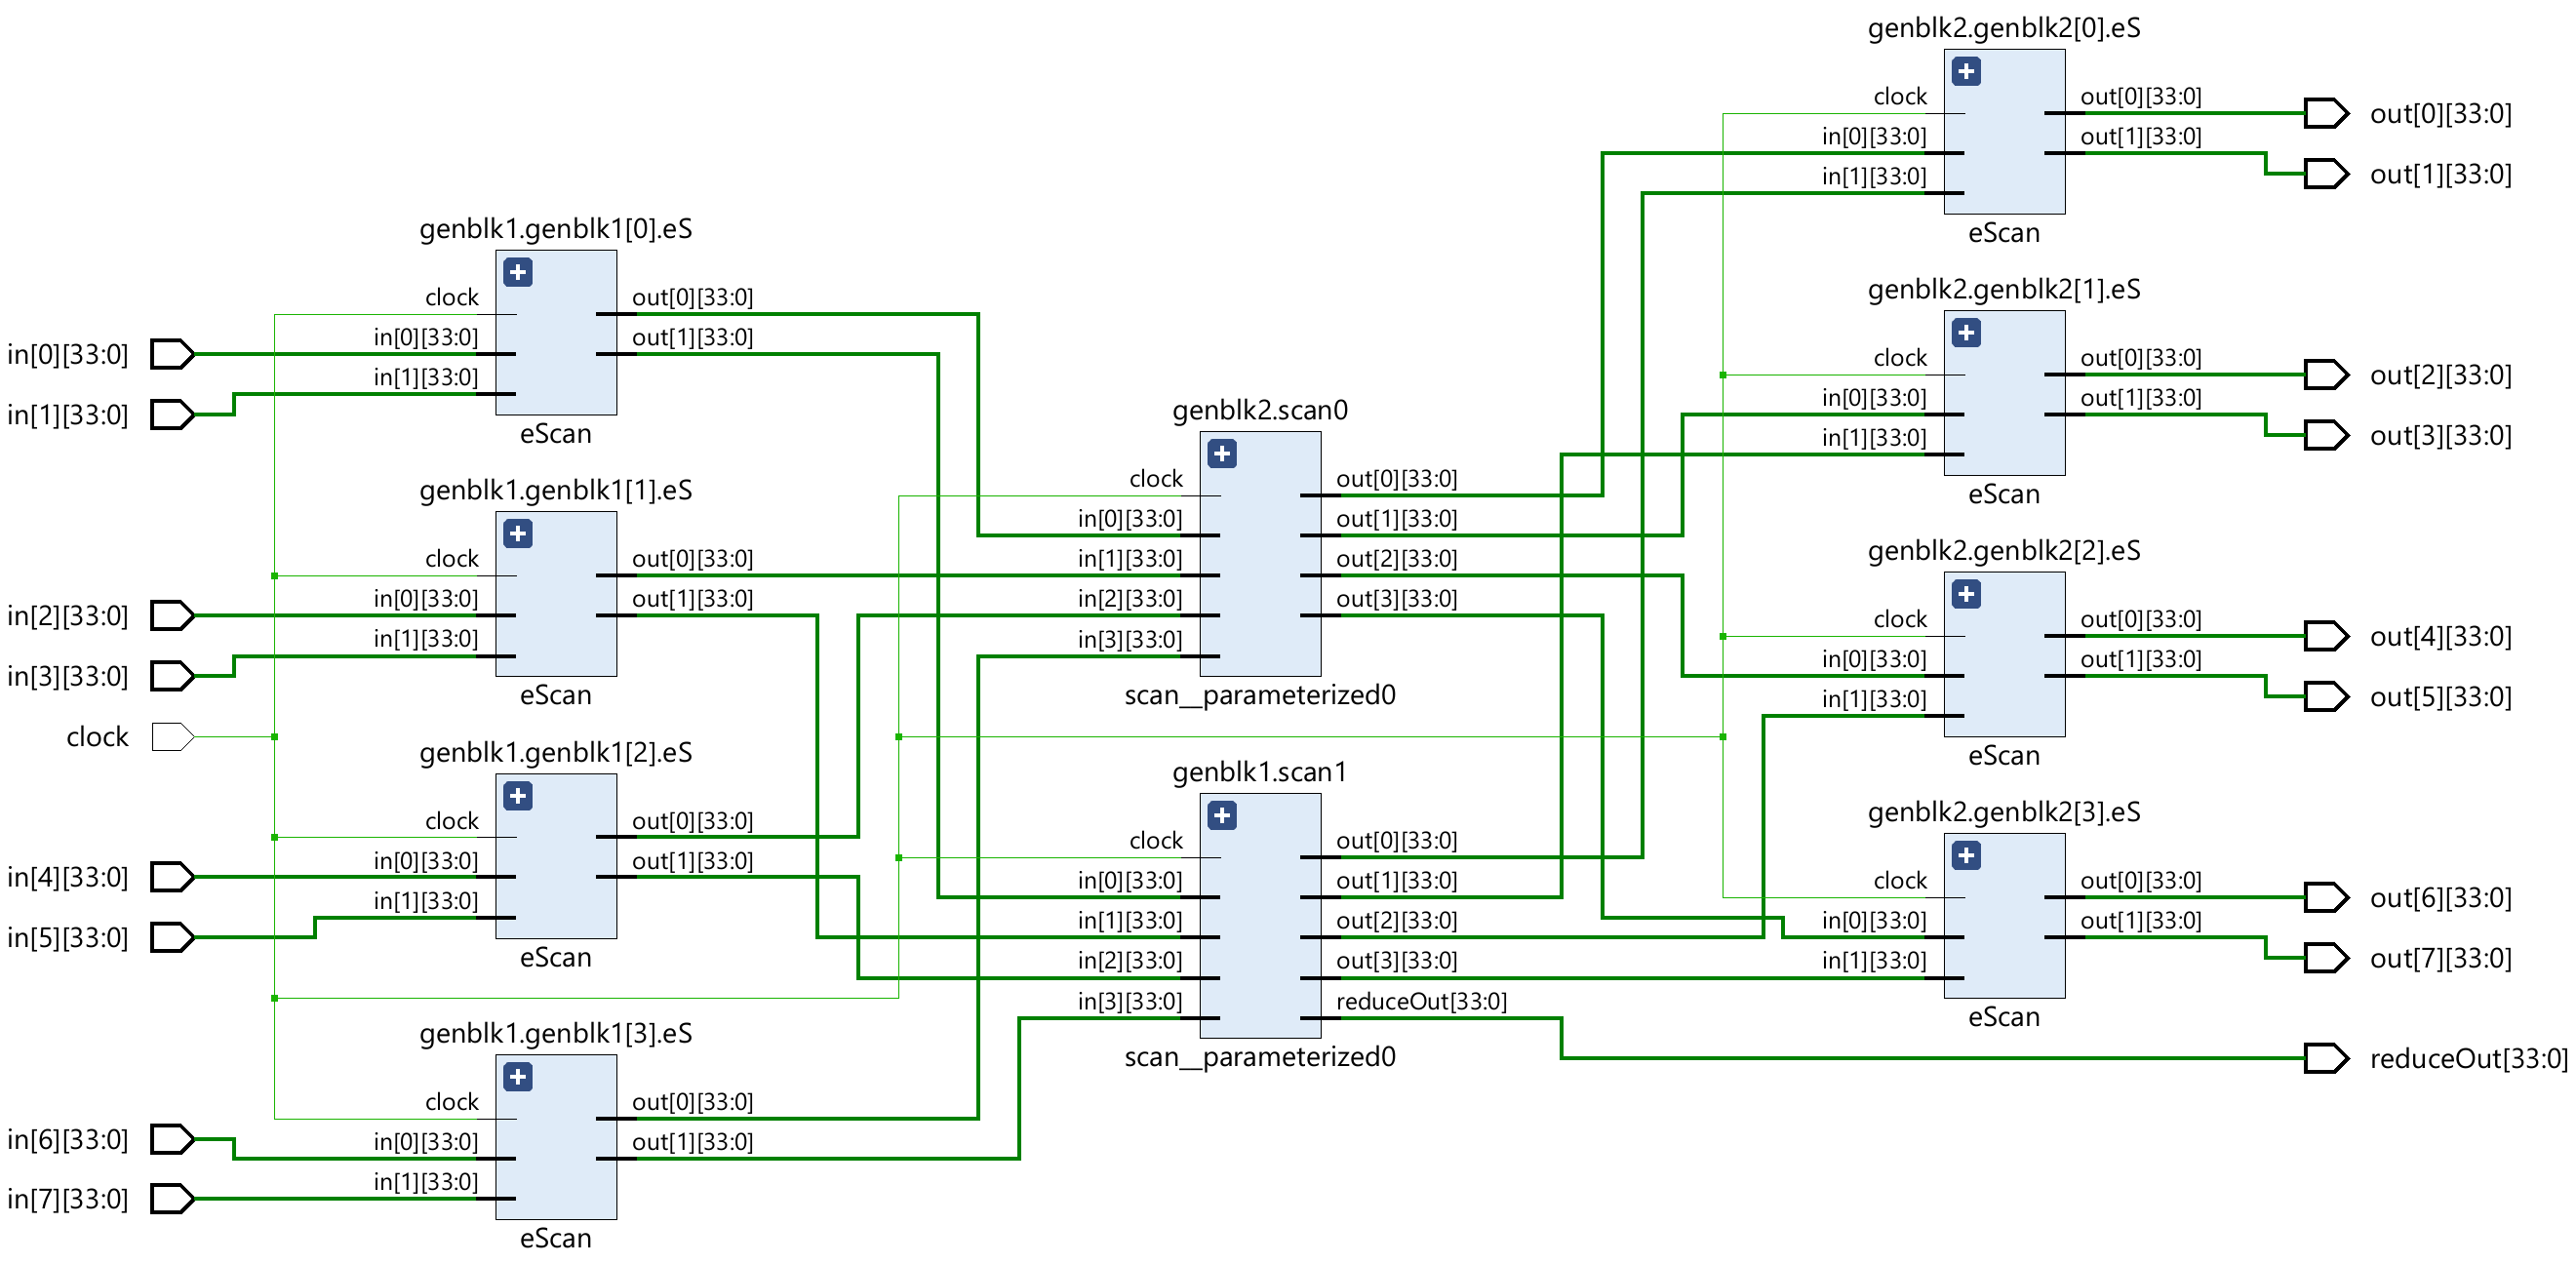
\includegraphics[width=\textwidth]{Images/scanRedTop.png}
    {\small {\bf a.}}
    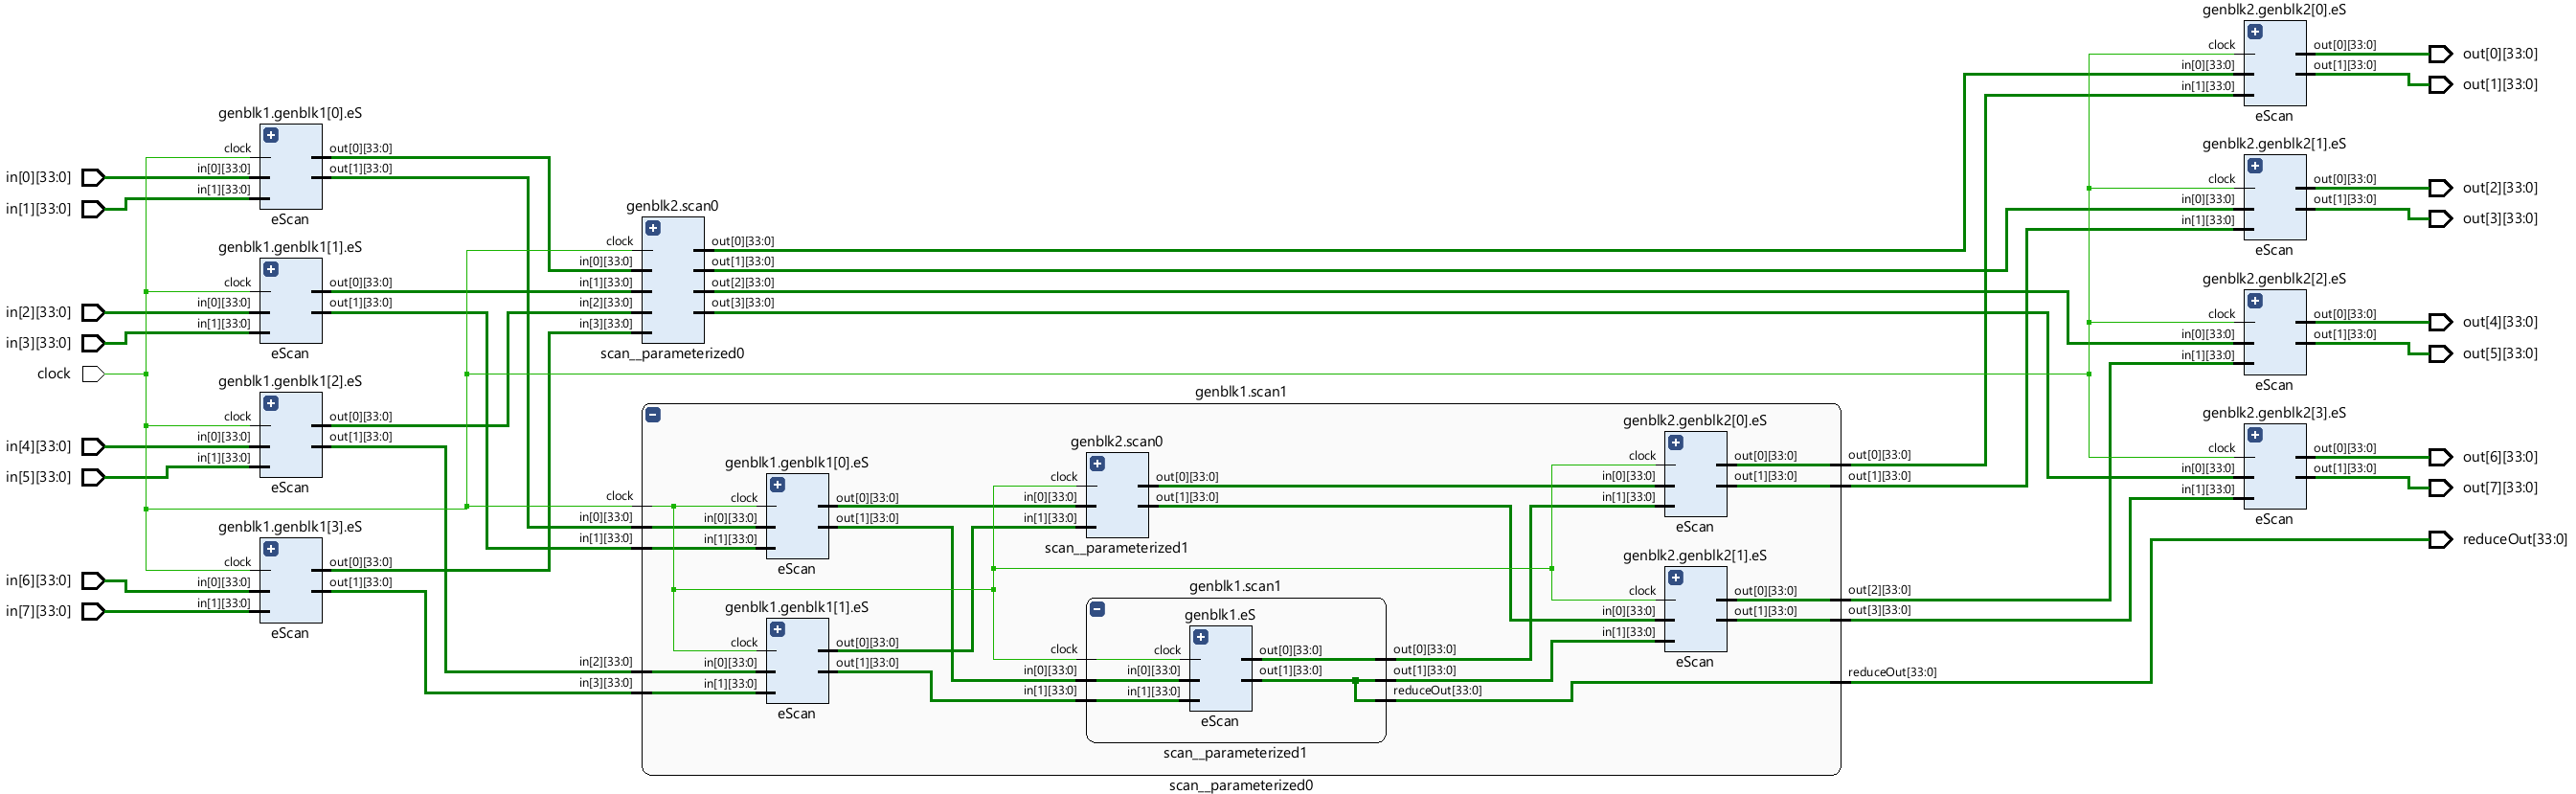
\includegraphics[width=\textwidth]{Images/scanRed.png}
   {\small  {\bf b.}}
    \caption{An 8-input scan circuit with the output for the reduction function. {\bf a}. The top module. {\bf b}. Detailed representation to emphasize {\tt reduceOut}. }
    \label{fig:scanRedTop}
\end{figure}
\end{comment}


We use the term {\em scan} by extension, starting from the already established use for prefix-type networks.

\begin{definition}
Let be an associative and commutative  operation, {\tt OP}. OP-prefix computation is defined on the scalar vectors, $[s_0 \; s_1 \; \ldots \; s_{n-1}]$ and returns the vector $[p_0 \; p_1 \; \ldots \; p_{n-1}]$, where:
$$ p_i = OP_0^i s_i$$

$\diamond$
\end{definition}
\begin{exemplu}
For OP arithmetic sum we have addPrefix:
$$p_0 = s_0$$
$$p_1 = p_0 + s_1 = s_0 + s_1$$
$$p_2 = p_1 + s_2 = s_0 +s_1 + s_2$$
$$\ldots$$
$$p_{n-1} = p_{n-2} + s_{n-1} = s_0 + s_1 + \ldots \; s_{n-1}$$

\placedrawing[H]{figures/09_13_scan_net.lp}{ An 8-input scan circuit adapted for an 8-input prefix operation.} {red}


$\diamond$
\end{exemplu}

{\bf Note}: the last output of $addPrefix$ is the output of $sumReduce$, thus justifying the simplified representation of the two loops in Figure \ref{secondLoop}.

The size of the pipeline implemented Scan network is in $O(p \times log \; p$, and the depth is in $O(log \; p$. Therefore, the size of the MapScanReduce structure is in $O(p \times log \; p$.

\subsection{Architectural additions}\label{scanEx}

The system architecture is completed by adding the second global loop, with  specific functions exemplified as follows:
\begin{description}
    \item[{\tt ADDPX(Vi)}:] add prefix returns a vector whose components are:\\
        $addPx_j \Leftarrow \sum_{j=0}^{j} (b_j ? s_{ij} : 0)$ for $j = 0, \ldots, p-1$ \\
         {\bf Example} of use: {\tt V2 <= ADDPX(V1)} 
    \begin{verbatim}
    For:        B  = [1 1 1 0 0 1 0 0]
                V1 = [2 3 1 4 3 5 2 0]
    results:    V2 = [2 5 6 6 6 11 11 11]
    \end{verbatim}
    \item[{\tt SPLIT(Vi)}:] return a vector with the selected components left aligned and the unselected component right aligned  \\
     {\bf Example} of use: {\tt V2 <= SPLIT(V1)} 
    \begin{verbatim}
    For:        B  = [0 1 1 0 0 1 0 0]
                V1 = [2 3 1 4 3 5 2 0]
    results:    V2 = [3 1 5 2 4 3 2 0]
    \end{verbatim}
\end{description}


\section{The mathematical model of partially recursive functions\index{partial recursive functions; defined by Stephen Kleene as a mathematical computational model}}

When we closed the fourth loop, starting from combinational circuits, we had the pleasant encounter with the mathematical model of the Turing Machine. Does a similar encounter await us with the closing of the two loops over a cellular automaton? Yes. It is a mathematical model proposed independently in the same year as the Turing Machine: the model of {\bf {\em partially recursive functions}} proposed by Stephen Kleene\index{Kleene, Stephen (1909-1994):  founder of  recursion theory, which subsequently helped to provide the foundations of theoretical computer science} \cite{Kleene36}.

\begin{definition}\label{parrec}
Let be the positive integers $x,y,i \in \mathbb{N}$ and the vector $\vec{x} = \langle x_0, x_1, \ldots, x_{n-1} \rangle \in \mathbb{N}^n$. Any partial recursive function $f: \mathbb{N}^n \rightarrow \mathbb{N}$ can be computed using three {\bf {\em initial functions}}:
\begin{itemize}
\item $ZERO(x) = 0:$ the variable $x$ takes the value {\bf zero}
\item $INC(x) = x+1:$ {\bf increment}s the variable $x \in \mathbb{N}$
\item $SEL(i, \vec{x}) = x_i:$ $i$ {\bf select}s the value of $x_i$ from the vector of positive integers $\vec{x}$
\end{itemize}
and the application of the following three {\bf {\em rules}}:
\begin{itemize}
\item {\bf Composition:}  $f(\vec{x}) = g(h_0(\vec{x}), \ldots, h_{p-1}(\vec{x}))$,
    where:  $f: \mathbb{N}^n \rightarrow \mathbb{N}$ is a total function if  $g: \mathbb{N}^p \rightarrow \mathbb{N}$ and  $h_i: \mathbb{N}^n \rightarrow \mathbb{N}$, for $i = 0,1, \ldots p-1$, are total functions
\item {\bf Primitive recursion:} $f(\vec{x},y) = g(\vec{x}, f(\vec{x}, (y-1)))$,  with $f(\vec{x},0) = h(\vec{x})$
    where:  $f:  \mathbb{N}^{n+1} \rightarrow  \mathbb{N}$ is a total function if $g:  \mathbb{N}^{n+1} \rightarrow  \mathbb{N}$ and $h:  \mathbb{N}^n \rightarrow  \mathbb{N}$ are total functions.
\item {\bf Minimization:} $f(\vec{x}) = \mu_y[g(\vec{x},y) = 0]$,
    which means: the value of the function  $f:  \mathbb{N}^{n} \rightarrow  \mathbb{N}$ is the smallest $y$, {\bf {\em if any}}, for which the function $g:  \mathbb{N}^{n+1} \rightarrow  \mathbb{N}$ takes the value $g(\vec{x},y) = 0$.
\end{itemize}

$\diamond$
\end{definition}

If we follow the previous definition, we will identify the initial functions with those directly realized by simple combinational circuits:
\begin{itemize}
    \item ZERO: implemented by generating a constant value
    \item INC: implemented as the increment circuit
    \item SEL: implemented as the multiplexer circuit
\end{itemize}
while the composition rule is implemented by the circuit represented in Figure \ref{compCirc}.

\placedrawing[h]{figures/14_9_compositionCircuit.LP}{{\bf The circuit version of composition.} {\small It is a two-layer construct: the parallel expanded {\em map} layer serially connected with the $log$-dept {\em reduction} layer.}}{compCirc}

The similarity between Figures \ref{firstLoop} and \ref{compCirc} encourages us to hope that both primitive recursion and minimization can find implementations in structures that we can physically realize with cellular constructions. Indeed, by composing {\em map composition} functions (see Figure \ref{compCirc}) one can obtain the purely theoretical construction in Figure \ref{2loops} (for details see \cite{Stefan00}). It is a theoretical one because is extended indefinitely to right for two reasons:
\begin{enumerate}
    \item we not know for how big $y$ a primitive recursion  computation is requested
    \item we not know for how big $y$, if any, the computation of a partial recursive function ends.
\end{enumerate}
While for the primitive recursion functions the value of $y$ is known at the beginning of computation, for the partial recursive functions the value of $y$, if any, is the result of the computation. For computing primitive recursive functions only  the map composition with the reduction network are sufficient, while for partial functions adding the scan network is mandatory. The simplest form of  the reduction network is one which provide the Boolean bitwise OR of the input components. For the scan network the minimal function receives a Boolean vector and provides the Boolean vector {\tt FIRST} which highlights only the first component having the value 1.

\placedrawing[h]{figures/14_10_partialRecursiveCircuit.lp}{{\bf The circuit version of the enhanced composition}. {\small In the map composition right connections are added considering specific map compositions. The scan circuit, a $log$-layer map compositions, is connected with the generic map composition.}}{2loops}

The theoretical structure in Figure \ref{2loops} can be transformed into an implementable one by adding a sequencer that converts the size of the structure into execution time. This becomes possible due to the local memories in each cell $M_i$. The result is a structure like the one in Figure \ref{secondLoop}, a structure that can be considered an {\bf {\em abstract model for a parallel computing system}}.


\section{Heterogeneous Computing\index{heterogeneous computing system: a host computer for the complex computation using a hardware accelerator for the intens computation}}

The main application of the MapScanReduce structure is in heterogeneous computing were the distinction between complex computing and intense computing is meaningful.

\subsection{Complexity vs. intensity in computation\index{complexity!complexity vs. intensity in computation}}

let's define the two types of computations. In this respect, we use the {\em algorithmic complexity} \cite{Chaitin70} which helps us make the necessary distinction between size and complexity.

\begin{definition}
The {\bf {\em algorithmic complexity}} of an entity is given by the length of its shortest description.

$\diamond$
\end{definition}

\begin{definition}
An entity is complex when its size is in the same magnitude order with its algorithmic complexity, and is simple when with a size in $O(f(N))$ its complexity remains in $O(1)$.

$\diamond$
\end{definition}

Now, regarding computation the following two definitions can be accepted.

\begin{definition}
Complex computation is characterized by an execution time proportional to the number of lines of executable code by which it is described.

$\diamond$
\end{definition}

\begin{definition}
The intensive, simple computation is described by a constant number, in $O(1)$, of lines of executable code, independent of the execution time which is in $O(f(N))$, where $N$ is used to define the size of the precessed data.

$\diamond$
\end{definition}

The previous definitions follow the algorithmic complexity \cite{Chaitin70} definition stating  mainly that the complexity of a computation is given by the length of its shortest description. While for complex computation the Turing tax can be reduced using {\em instruction-level parallelism}, for simple, intense computation a promising solution is  {\em cellular parallelism}. A typical example for intense, simple computation is the multiplication of $N \times N$ matrices performed on a mono-core engine in $O(N^3)$ time. An accelerator with $p$ execution units (cells) is expected to reduce execution times by at least $O(p/log \; p)$ times. It runs a constant (independent of N) code size.

\subsection{Heterogeneous system}\label{hetCompSystem}

Heterogeneous computing takes into account the distinction between complex and intensive computing. This segregation is possible using a system in which a single-core computer, instantiated as a HOST, uses a library of functions implemented in hardware in a MapScanReduce structure to perform complex calculations. In Figure \ref{hetSyst}, such a heterogeneous computing system is represented.

\placedrawing[h]{figures/09_10_heterogeneous_system.lp}{}{hetSyst}

The two types of computation, complex and intensive, can be performed efficiently if we have adequate hardware for each. This is what we achieve with a heterogeneous system. The problem is the acceleration that we obtain for an application in which we have a mixture of intensive and complex computation. Evaluating the performance of the accelerator is not enough because what is important is the total performance that is obtained by taking into account the execution time associated with the complex computation, which cannot be accelerated in the host, and the execution time associated with the intensive computation subject to acceleration in the accelerator.

Since the 1960s, with the advent of the first parallel computers, the problem of limited acceleration due to the weight of complex calculations has arisen. The limitation was expressed by Amdahl's Law.

Amdahl's law, named after  Gene Amdahl,  was introduced  at a conference in 1967 \cite{amdahl1967}, and can be used in parallel computing to predict the limit of the theoretical speedup when using heterogeneous computation. It is formulated in the following way:
$$A_{host+accelerator} = \frac{1}{(1-w_{intenseComp}) + \frac{w_{accelerator}}{A_{accelerator}}}$$
where:
\begin{description}
    \item[$A_{host+accelerator}$:] represents the overall acceleration of the heterogeneous system running an application
    \item[$A_{accelerator}$:] represents the acceleration obtained by the accelerator running the intense part of the application
    \item[$w_{intenseComp}$:] the weight of the intense computation in the application expressed by a subunit number
\end{description}
We can highlight two limiting cases:
\begin{enumerate}
    \item computation is dominated by the complex computation: with $w_{intenseComp} = 0.05$ and $A_{accelerator} = 1000$ results $A_{host+accelerator} = 1.05$
    \item computation is dominated by the intense computation: $w_{intenseComp} = 0.95$ and $A_{accelerator} = 1000$ results $A_{host+accelerator} = 19.62$
\end{enumerate}
In the limiting cases, for $w_{accelerator} = 1$ we have $A_{host+accelerator} = A_{accelerator}$, while for $w_{accelerator} = 0$ we have $A_{host+accelerator} = 1$.

\subsection{Programming a heterogeneous system}

Concerning the programming of multicellular processors, which have seen a rapid proliferation primarily driven by corporate considerations, the scientific community has yet to universally embrace effective solutions. The challenge arises from the prioritization of hardware criteria that promoted multi- and many-cell solutions without sufficient regard for their programmability. This is due to:
{\small
\begin{quote}
{\em "the semiconductor industry threw the equivalent of a Hail
Mary pass when it switched from making microprocessors run faster to
putting more of them on a chip—doing so without any clear notion of how
such devices would in general be programmed. The hope is that someone
will be able to figure out how to do that, but at the moment, the ball is still in the air."} \cite{Patterson10}
\end{quote}
}

%It seems that the solution is not specific languages for parallel structures:

It appears that the solution does not entail specific languages tailored for parallel structures:
{\small
\begin{quote}
{\em "The software span connecting applications to hardware relies more on parallel software architectures than on parallel programming languages. Instead of traditional optimizing compilers, we depend on autotuners, using a combination of empirical search and performance modeling to create highly optimized libraries tailored to specific machines."} \cite{Asanovic09}
\end{quote}
}

As a result, our heterogeneous approach imposes, for efficiency, a three level programming system:
\begin{enumerate}
    \item ACCELERATOR-level programming is done in assembly language providing a highly optimized library of primitives.
    \item HOST-level libraries  developed  in a high-level programming language  based on primitives provided by ACCELERATOR.
    \item HOST-level programming running  in a high-level programming language based on "highly optimized libraries tailored to specific machines".
\end{enumerate}

\subsubsection{Accelerator-level programming}

In Table \ref{ops} is listed partially the set of operations performed at the accelerator-level.


\begin{table}[h]
	\centering                       
	\caption{Accelerator-level operations}           
	\label{ops}       % Label

	\begin{tabular}{|l|l|} \hline  % Your table
		Operation & Description  \\ \hline \hline
        ACTIVATE    & activate all cells: $b_i=1$ for $i = 0,1,\ldots ,p1-$ \\ \hline
        WHERE(Vi=0) & where scalar in Vi is zero, cell remains active \\ \hline
        ELSEWHERE & cells inactivated by the last WHERE become active \\ \hline
        ENDWHERE & vector B takes the value before the most recent WHERE \\ \hline
		ADD(Vj,Vk) & add vectors Vj and Vk in each active position   \\ \hline
		MULT(Vj,Vk) & multiply vectors Vj and Vk in each active position   \\ \hline
        AND(Vj,Vk) & bitwise AND of vectors Vj and Vk in each active position  \\ \hline
        OR(Vj,Vk) & bitwise OR of vectors Vj and Vk in each active position  \\ \hline
        XOR(Vj,Vk) & bitwise XOR of vectors Vj and Vk in each active position  \\ \hline
        VAL(s) & generate a vector with value s in each active position \\ \hline
        ADDRED(Vi) & active components of Vi are submitted to reduction add \\ \hline
        MINRED(Vi) & active components of Vi are submitted to reduction minimum \\ \hline
        MAXRED(Vi) & active components of Vi are submitted to reduction maximum \\ \hline
        ORRED(Vi) & active components of Vi are submitted to reduction logic OR \\ \hline
        ADDPX(Vi) & active components of Vi are submitted to prefix add function \\ \hline
        SHIFTRIGHT(Vi, leftIn) & shift right the component of Vi and insert leftIn \\ \hline
        SHIFTLEFT(Vi, rightIn) & shift left the component of Vi and insert rightIn \\ \hline
        ROTATERIGHT(Vi) & rotate right the component of Vi \\ \hline
        ROTATELEFT(Vi) & shift left the component of Vi \\ \hline
	\end{tabular}

\end{table}


\subsubsection{Library of primitives: an example}\label{library}

One of the most used library of function contains linear algebra functions. In the following few of the most used linear algebra functions are described to exemplify the intense functions appropriate to be implemented on a MapScanReduce architecture.

\paragraph{Matrix} is a rectangular array of $n$ lines and $m$ columns scalar components, as follows:
\[
{\bf M} = \begin{bmatrix}
    s_{11} & s_{12} & s_{13} & \ldots & s_{1n} \\
    s_{21} & s_{22} & s_{23} & \ldots & s_{2n} \\
    \ldots & \ldots & \ldots & \ldots & \ldots \\
    s_{m1} & s_{m2} & s_[m3] & \dots  & s_{mn}
    \end{bmatrix}
\]

\paragraph{Identity matrix} is a matrix working as the scalar 1 in the arithmetic multiplication and division; it has 1s on the main diagonal as follows:
\[
{\bf I} = \begin{bmatrix}
    1 & 0 & 0 & \ldots & 0 \\
    0 & 1 & 0 & \ldots & 0 \\
    \ldots & \ldots & \ldots & \ldots & 0 \\
    0 & 0 & 0 & \dots  & 1
    \end{bmatrix}
\]

\paragraph{Row Vector} is a linear array of $n$ scalars, as follows:
\[
V = \begin{bmatrix}
    s_{1} & s_{2} & s_{3} & \ldots & s_{n} 
    \end{bmatrix}
\]

\paragraph{Column Vector} is a linear array of $m$ scalars, as follows:
\[
W = \begin{bmatrix}
    s_{1} \\
    s_{2} \\
    \ldots \\
    s_{m} 
    \end{bmatrix}
\]

\paragraph{Inner or dot product} of two vector provides a scalar as the sum of matching members products, as follows:
\[
V \cdot W = \begin{bmatrix}
    s_{1} & s_{2} & s_{3} & \ldots & s_{n} 
    \end{bmatrix}
    \cdot
    \begin{bmatrix}
    t_{1} \\
    t_{2} \\
    \ldots \\
    t_{n} 
    \end{bmatrix}
    = \sum_{1}^{n} s_i \times t_i
\]



\begin{exemplu} Let be the vectors {\tt V1 = [1 2 3 4]} and {\tt V2 = [5 6 7 8]}. Their inner, dot or scalar product is: $$V1 \cdot V2 = 1 \times 5 + 2 \times 6 + 3 \times 7 + 4 \times 8 = 70$$

$\diamond$
\end{exemplu}

\paragraph{Matrix-vector multiply} provide a vector of the dot products between the lines of the matrix and the vector, as follows:

\[
{\bf M} \cdot W = \begin{bmatrix}
    s_{11} & s_{12} & s_{13} & \ldots & s_{1n} \\
    s_{21} & s_{22} & s_{23} & \ldots & s_{2n} \\
    \ldots & \ldots & \ldots & \ldots & \ldots \\
    s_{m1} & s_{m2} & s_[m3] & \dots  & s_{mn}
    \end{bmatrix}
    \cdot
    \begin{bmatrix}
    t_{1} \\
    t_{2} \\
    \ldots \\
    t_{n} 
    \end{bmatrix}
    = 
    \begin{bmatrix}
    V_{1} \\
    V_{2} \\
    \ldots \\
    V_{m} 
    \end{bmatrix}
    \cdot W
    = 
    \begin{bmatrix}
    V_{1} \cdot W \\
    V_{2} \cdot W \\
    \ldots \\
    V_{m} \cdot W
    \end{bmatrix}
\]


\begin{exemplu}
Let be the matrix
\[
M = \begin{bmatrix}
    1 & 2 & 3 \\
    4 & 5 & 6\\
    7 & 8 & 9
    \end{bmatrix}
\]
and the vector 
\[
V = \begin{bmatrix}
    10 \\
    11 \\
    12 
    \end{bmatrix}
\] 
their product is:
\[
M \times V = \begin{bmatrix}
    1 & 2 & 3 \\
    4 & 5 & 6\\
    7 & 8 & 9
    \end{bmatrix}
    \cdot
    \begin{bmatrix}
    10 \\
    11 \\
    12
    \end{bmatrix}
    = 
    \begin{bmatrix}
    1 \times 10 + 2 \times 11 + 3 \times 12 \\
    4 \times 10 + 5 \times 11 + 6 \times 12  \\
    7 \times 10 + 8 \times 11 + 9 \times 12 
    \end{bmatrix}
    = 
     \begin{bmatrix}
    68 \\
    167 \\
    326
    \end{bmatrix}
\]

$\diamond$
\end{exemplu}

\paragraph{Matrix multiplication} of two matrices ${\bf M_1}$ and ${\bf M_2}$ provides a matrix ${\bf M}$ whose lines a contains the dot products of a column, starting with the first column, form ${\bf M_2}$ with each lines from ${\bf M_1}$ starting with the first line in ${\bf M_1}$. The number of lines in ${\bf M_1}$ must be the same with the number of columns in ${\bf M_2}$. The general form is:

\[
{\bf M_1} \cdot {\bf M_2} = 
    \begin{bmatrix}
    s_{11} & s_{12} & s_{13} & \ldots & s_{1k} \\
    s_{21} & s_{22} & s_{23} & \ldots & s_{2k} \\
    \ldots & \ldots & \ldots & \ldots & \ldots \\
    s_{m1} & s_{m2} & s_[m3] & \dots  & s_{mk}
    \end{bmatrix}
    \cdot
    \begin{bmatrix}
    t_{11} & t_{12} & t_{13} & \ldots & t_{1n} \\
    t_{21} & t_{22} & t_{23} & \ldots & t_{2n} \\
    \ldots & \ldots & \ldots & \ldots & \ldots \\
    t_{k1} & t_{k2} & t_[k3] & \dots  & t_{kn}
    \end{bmatrix}
    =
\]
\[
    =
    \begin{bmatrix}
    V_{1} \\
    V_{2} \\
    \ldots \\
    V_{m} 
    \end{bmatrix}
    \cdot
    \begin{bmatrix}
    W_{1} & W_{2} & W_{3} & \ldots & W_{n} 
    \end{bmatrix}
    =
    \begin{bmatrix}
    V_{1} \cdot W_{1} & V_{1} \cdot W_{2} & V_{1} \cdot W_{3} & \ldots & V_{1} \cdot W_{n} \\
    V_{2} \cdot W_{1} & V_{2} \cdot W_{2} & V_{2} \cdot W_{3} & \ldots & V_{n} \cdot W_{n} \\
    \ldots & \ldots & \ldots & \ldots & \ldots \\
    V_{m} \cdot W_{1} & V_{m} \cdot W_{2} & V_{m} \cdot W_{3} & \ldots & V_{m} \cdot W_{n} 
    \end{bmatrix}
\]


Let us consider the simplest, most intense computation of multiplying matrices.
\includeverilogcode[caption={Matrix multiplication in Python.  File: matrix\_multiplication.py. }, 
                    label={lst:matrixMultiplication}, 
                    firstline=1, 
                    firstnumber=1, 
                    lastline=68]
                    {\verilogSourceDir/A14_matrix_multiplication.py}

The execution time of this program on a mono-core processor is proportional with the number of clock cycles:
$$range(cols\_B) \times range(cols\_B) \times range(cols\_A)$$
which means, for example: if $range(cols\_B) = range(cols\_B) = range(cols\_A) = 1024$, the execution time is proportional with $1024^3 \simeq 10^9$.

However, in high-level languages like Python there are function libraries for frequently used functions like matrix multiplication. In this case the program takes the simplified form below:
\includeverilogcode[caption={Matrix multiplication in Python using a library of function.  File: matrixMultiplication.py. }, 
                    label={lst:matrixmultiplication}, 
                    firstline=1, 
                    firstnumber=1, 
                    lastline=68]
                    {\verilogSourceDir/A14_matrixMultiplication.py}

The line {\tt result = np.dot(A,B)} access, when the program runs on a mono-core processor, a highly optimized program (usually written in assembly language) for the matrix multiplication operation. In a heterogeneous system, instead of calling a program from library, is accessed a function performed hardware accelerated by the associated accelerator.

\begin{exemplu}
Let see how looks the algorithm for multiplying two $n \times n$ matrices, {\tt A} and {\tt B}. The transposed matrix of B is {\tt T}. Each matrix is represented by vectors in a Map with $p\geq n$.
{\em 
\includeverilogcode[caption={Matrix multiplication algorithm using a hardware accelerator.  }, 
                    label={lst:matrixMult}, 
                    firstline=1, 
                    firstnumber=1, 
                    lastline=68]
                    {\verilogSourceDir/A14_matrixMult}
}

Because the previous algorithm works with vectors, instead of the three embedded lops in the Python program {\tt matrix\_multiplication.py}, in the {\tt matrix\_multiplication} algorithm {\bf {\em there are only two embedded loops}}. Besides this good news, there is also a bad news: the operation repeated $n^2$ times is executed in time belonging to $O(log \; n)$ cycles. Because the line {\tt result[i][j] += A[i][k] * B[k][j]} in the Python program is executed in constant time, the acceleration provided by the MapScanReduce accelerator is only of $n/log_2 n$. (A well-designed algorithm can avoid this bad news, but this topic goes beyond the level at which we approach parallelism problems.)

$\diamond$
\end{exemplu}

\paragraph{Matrix transpose} applied to the matrix $M$ is $M^T$ with the lines equal with the columns of $M$.

\begin{exemplu}
Let be the matrix:
\[
M = \begin{bmatrix}
    1 & 2 & 3 \\
    4 & 5 & 6\\
    7 & 8 & 9
    \end{bmatrix}
\]
Its transpose is:
\[
M^T = \begin{bmatrix}
    1 & 4 & 7 \\
    3 & 5 & 8\\
    3 & 6 & 9
    \end{bmatrix}
\]

$\diamond$
\end{exemplu}

To describe the algorithm for square matrix transpose, we will define the concept of {\bf {\em pseudo diagonal}} of a square matrix.

\begin{definition}
{\em
Let be the square matrix
\[{\bf M} =
\begin{bmatrix}
    v_{00} & v_{01} & \dots  & v_{0 \; m-1}\\
    v_{10} & v_{11} & \dots  & v_{1 \; m-1}\\
    \vdots & \vdots & \ddots & \vdots\\
    v_{m-1 \; 0} & v_{m-1 \; 1} & \dots  & v_{m-1 \; m-1}
    \end{bmatrix}
\]
where $$PD(k,{\bf M}) = [v_{(0+k)_{mod \; m} \; 0} \; v_{(1+k)_{mod \; m} \; 1} \ldots v_{(m-1+k)_{mod \; m} \; m-1}]$$ is the $k$-th {\bf {\em pseudo-diagonal}} in the matrix {\bf M}. (The 0-th pseudo-diagonal is the main diagonal.)
}

$\diamond$
\end{definition}

A vector algorithm for matrix transpose uses the pseudo-diagonal concept, as follows:

{\footnotesize
\begin{shaded*}
\begin{lstlisting}[language=Verilog, caption= , morekeywords={activate, where, wait, loop, repeat, doInParallel, for}]
/****************************************************************************
    Algorithm for matrix transpose
        Initial matrix, V, with components: v(i,j), for i,j = 0, 1, ... m-1
        Final matrix, W, with components:   w(i,j), for i,j = 0, 1, ... m-1
        Working vector: A = [a(0) a(1) ... a(m-1)]
    Note: addition and subtract operations are modulo m operations
****************************************************************************/
for(k=0; k<m; k=k+1) begin
  (step 1) A <= [v(0+k,0)v[1+k,1]...v[m-1+k,m-1] // A <= PD(k.V)
  (step 2) A <= [a(0-k)a(1-k)...a(m-1-k)]        // A rotate k times right
  (step 3) for(j=0; j<m; j=j+1) w(j+k,j) <= a(j) // PD(m-k,W) <= A
end
\end{lstlisting}
\end{shaded*}
}


\begin{exemplu}
Let's consider the $4 \times 4$ matrix V. Its transposed form is computad as follows:

{\small
\begin{verbatim}
    Initial                                                        Final
                          k = 0    k = 1    k = 2    k = 3
 V: 0 1 2 3     (step 1) 0 5 A F  4 9 E 3  8 D 2 7  C 1 6 B     V: 0 1 2 3
    4 5 6 7                                                        4 5 6 7
    8 9 A B                                                        8 9 A B
    C D E F                                                        C D E F

                (step 2) 0 5 A F  3 4 9 E  2 7 8 D  1 6 B C

 W: x x x x     (step 3) 0 x x x  0 4 x x  0 4 8 x  0 4 8 C     W: 0 4 8 C
    x x x x              x 5 x x  x 5 9 x  x 5 9 D  1 5 9 D        1 5 9 D
    x x x x              x x A x  x x A E  2 x A E  2 6 A E        2 6 A E
    x x x x              x x x F  3 x x F  3 7 x F  3 7 B F        3 7 B F
\end{verbatim}
 }

$\diamond$
\end{exemplu}




\begin{exemplu}
In Table \ref{prim} is listed an example for a library of primitives:  FLA 0.1. It can be used to develop in a high level language on HOST a linear algebra library. The library of primitives contains functions defined on data structures -- vectors and matrices --- limited to the size of the array of cells  Map, i.e., $p$-component vectors and $p \times p$ matrices. Programs developed on HOST adapt linear algebra operations defined on data of any size to linear algebra operations defined on accelerator dimensions. In this way, a speedup is obtained that depends on $p$ even if the order of magnitude of the computation time remains the same, i.e., the execution time of matrix multiplication, for example, remains the same, in $O(n^3)$ for matrices of $n \times n$.

{\em
\begin{table}[H]
	\centering                       
	\caption{Library of linear algebra primitives, FLA 0.1,  for $p \times p$ matrices and $p$-component vectors on a $p$-cell MapScanReduce accelerator. }           
	\label{prim}       % Label
	\begin{tabular}{|p{0.22\textwidth}|p{0.55\textwidth}|p{0.075\textwidth}| } \hline  % Your table
		{\bf FLA 0.1 functions}    & {\bf Description}                                 & {\bf Time}  \\ \hline \hline
        hSTART            & start the cycle counter on sequencer's            & $O(1)$ \\ \hline
        hSTOP             & stop the cycle counter on sequencer's             & $O(1)$ \\ \hline
        hINTRQ            & interrupt request                                 & $O(1)$ \\ \hline
        hVGENN(d,v)       & generate in V(d) uniform vector, [v v ... v]                                    & $O(1)$ \\ \hline
        hVGENX(d)         & generate in V(d) index vector, [0 1 ... p-1]                                    & $O(1)$ \\ \hline
        hMAIN(d,v)        & generate, starting with V(d), matrix with main diagonal of values v             & $O(p)$ \\ \hline
        hSQGENN(d)        & generate, starting with V(d) = [0 0 ... 0], matrix with incremental lines       & $O(p)$ \\ \hline
        hSQGENX(d)        & generate, starting with V(d) = [0 1 ... p-1], matrix with incremental lines     & $O(p)$ \\ \hline
        hPRANDOM(d)       & generate, starting with V(d), pseudo-random matrix                              & $O(p)$ \\ \hline
        hMSEND(a,s)       & send to host a s-line matrix starting with V(a)                                 & $O(ps)$ \\ \hline
        hMGET(a,s)        & get from host a s-line matrix starting with V(a)                                & $O(ps)$ \\ \hline
        hTRANS(d,l)       & transpose matrix starting at V(l) in matrix starting at V(d)                    & $O(p^2)$ \\ \hline
        hSQMADD(d,l,r)    & add starting from V(d) the matrices starting from V(l) and V(r)                 & $O(p)$ \\ \hline
        hSQMVMULT(m,v,d)  & multiply in V(d) the matrix starting at V(m) with the vector V(v)               & $O(p)$ \\ \hline
        hSQMMULT(d,l,r)   & multiply in matrix starting with V(d) matrices starting with V(l) and V(r)      & $O(p^2)$ \\ \hline
        hSQMMAC(d,l,r)    & multiply and add in matrix starting with V(d) matrices starting with V(l) and V(r)      & $O(p^2)$ \\ \hline
	\end{tabular}
\end{table}
}

$\diamond$
\end{exemplu}

\begin{exemplu}
Let us consider an accelerator with $p=256$ and the program for multiply $1024 \times 1024$ matrices. Then, the HOST consider the multiplication of matrices of $4 \times 4$ matrices of $256 \times 256$ components. The acceleration compared to the computation without accelerator is:
$$\alpha = \frac{k_1 \times 1024^3}{k_2 \times 4^3 \times k_3 \times 256^2} = k \times 256 \in O(p)$$

$\diamond$
\end{exemplu}

\section{Parallel Computing Patterns\index{parallel computing patterns: recurring computational idioms for parallel architecture}}\label{parPatterns}

Multiplying matrices is a promising example for the capacity to perform in parallel with MapScanReduce accelerator intense computation. It would be interesting to investigate the acceleration capacity of the MapScanReduce framework for a wider range of applications. A good idea could be formed by looking at the computational patterns that have been highlighted in applications designed and run in the last decades. Let us start with the study carried out in \cite{McCool12} from which we use Figure \ref{parallelPatt} where 17 parallel computational patterns are presented. We will see that almost all of them can be performed using the accelerator MapScanReduce. We will not succeed in the case of those patterns that do not represent an intensive computation but a complex one.

\placedrawing[h]{figures/09_14_parallelPatterns.lp}{Parallel patterns \cite{McCool12}.}{parallelPatt}

We will analyze in turn how the 17 patterns revealed by McCool and his collaborators can be accelerated using the MapScanReduce structure. These patterns classifies in three categories:
\begin{enumerate}
    \item Map-Only patterns -- executed on {\bf {\em no global loop}} structure
    \begin{enumerate}
        \item Map-Reduce patterns -- executed on {\bf {\em one global loop}} structure
        \item Map-Scan -- executed on {\bf {\em one global loop}} structure
    \end{enumerate}
    \item Map-Scan-Reduce -- executed on {\bf {\em two global loops}} structure
\end{enumerate}

\subsection{Patterns with Map-Only Implemented with No Global Loop}

A first subset of patterns is the one that are implementable with the Controlled Cellular Automaton (see \ref{contrCellAut}) structure used as accelerator. Many of the patterns we consider are executed exclusively involving the Map section. For them to be executed, a sequence of Map operations is required each time.

\subsubsection{Map Pattern\index{parallel computing patterns!map pattern}}

From the list proposed by McCool \& Co., the Map pattern finds a direct counterpart in the accelerator we are evaluating. In Figure \ref{parallelPatt} the Map pattern is represented using green boxes, which represent data, and blue boxes, which represent hardware structure performing sequences of $bOp$s and $uOp$s. Overall the array of blue boxes represents a Map structure performing a {\tt MAPOP(Va,Vb,Vc,...)} on the vectors stored along the cells of the array. Thus, the Map pattern is has a direct correspondent in we can do with arithmetic \& logic vector operations. 

\begin{exemplu}
Let be an $8$-cell Map with 
\begin{verbatim}
    V10 = <x x x x x x x x>
    V12 = <2 4 7 1 8 4 5 2>
    V15 = <4 2 2 8 5 1 3 6>
\end{verbatim}
and we have to generate in the even indexed cells of V10 the sum of  the even indexed cell from V12 and V15 and in odd cells of V10 the difference between the odd cells of V12 and V15. The sequence of operations is:
\begin{verbatim}
    ACTIVATE            | B = <1 1 1 1 1 1 1 1>: set all cells active
    V2 <= VAL(1)        | V2 = <1 1 1 1 1 1 1 1>: load V2 with 1s
    V3 <= AND(IX,V2)    | V3 = <0 1 0 ... 1>: bwAND between IX and V2 
    WHERE(V3==0)        | B = < 1 0 1 ... 0>
    V10 <= ADD(V12,V15) | V10 = <6 x 9 x 13 x 8 x>
    ELSEWHERE           | B = <0 1 0 ... 1> 
    V10 <= SUB(V12,V15) | V10 = <6 2 9 -7 13 3 8 -4>
    ENDWHERE            | B = <1 1 1 1 1 1 1 1>
\end{verbatim}
The execution time of the previous sequence of operations does not depend on the number of cells, i.e., the execution time is in $O(1)$. The acceleration provided by this execution, compared with one performed by a mono-core engine, is in $O(p)$. The degree of parallelism si near 1, i.e., almost  in each clock cycle all cells are active. 

$\diamond$
\end{exemplu}

There are real premises for the acceleration obtained by using a Map array to be in $O(p)$, but more than that there are many cases when the acceleration is  {\bf {\em superlinear}} compared to a single-core structure, due to the control that is performed by SQ, control that in a single-core implementation is also the responsibility of the processor \cite{antonescu24a}.

\subsubsection{Stencil Pattern\index{parallel computing patterns!stencil pattern}}

The stencil pattern (depicted in  Figure \ref{parallelPatt}) is not directly implemented in the structure of the proposed accelerator, but can be efficiently programmed taking into account the fact that the input data structure is a matrix that can be loaded as part of the ${\bf M_{mp}}$ matrix. The finite neighborhood of each cell can be involved in the calculation of a new value in each cell very efficiently, because the values from the vertical vectors are in the same cell and a global shift operations allows access to the values from the horizontal vector. In fact, any finite neighborhood can be involved in updating  any value in ${\bf M_{mp}}$.

For example, let us consider the matrix stored in vectors from $V_0$ to $V_{n-1}$. Let us  consider a stencil computation in each cell of vector $V_i$ using as operands values from a type of neighborhood emphasized in Figure \ref{parallelPatt}: $s_{ij}$ as a central value, $s_{i(j-1)}, s_{i(j-2)}$ as values from the same vector positioned left, and $s_{i(j+1)}, s_{i(j+2)}$ positioned right, $s_{(i+1)j}, s_{(i+2)j}, s_{(i-1)j}, s_{(i-2)j}$ positioned in the same cell up two positions and down two positions.  The values to be used as operands are collected  in each cell and then submitted to a pure map sequence of operations which update the horizontal vector $V_i$ as follows:
\begin{verbatim}
    Vn     <= SHIFTRIGHT(Vi,0)
    V(n+1) <= SHIFTRIGHT(Vn,0)
    V(n+2) <= SHHIFTLEFT(Vi,0)
    V(n+3) <= SHHIFTLEFT(V(n+2),0)
    MAPOP(Vi,Vn,V(n+1),V(n+2),V(n+3),...)
\end{verbatim}
Because the update computation is done in parallel  for all the components of the horizontal vector $V_i$, the acceleration of the computation is in $O(p)$.

\subsubsection{Geometric Decomposition  Pattern\index{parallel computing patterns!geometric decomposition pattern}}

The geometric decomposition pattern works on configurable (overlapping) sub-collections  of data. In Figure \ref{parallelPatt}, four $5 \times 5$ scalars sub-collections are defined. If data is loaded in the accelerator's memory as a matrix of scalars, a sub-collection, $S(i,j,k,q)$, is a matrix loaded in ${\bf M_{mp}}$ between two horizontal vectors , $V_i$ and $V_j$, and two columns (vertical vectors), $C_k = [s_{0k} \; s_{1k} \ldots s_{m-1 \; k}]$ and $C_q = [s_{0q} \; s_{1q} \ldots s_{m-1 \; q}]$. The values for $i$ and $j$ are controlled by the program executed on the sequencer SQ, while the values of $k$ and $q$ are used by the {\em spatial selection} mechanism in Map. The $IX$ vector is used to delimit the index  of the vertical vectors applying spatial selection functions:
\begin{verbatim}
    WHERE(IX>=k)
    WHERE(IX<=q)
    MAPOP(Vi,V(i+1), ... V(j-1),V(j))
\end{verbatim}
Thus, any sub-collection is delimited in the matrix ${\bf M_{mp}}$, if $i,j,k,q \leq m,p$, in constant time. The degree of parallelism depends on the size of the sub-collections.

\subsubsection{Partition  Pattern\index{parallel computing patterns!partition pattern}}

The partition pattern corresponds to a geometric decomposition pattern without overlapping regions. See in Figure \ref{parallelPatt} a partition in four $4 \times 4$ scalars sub-collections. When dealing with sub-collections of varying sizes, it involves  {\em segmentation}. The same mechanisms for defining sections (sub-collections) used for geometric decomposition are considered for splitting, with the additional care to avoid overlap. We can take into account for the horizontal delimitations, in addition to those stated for the geometric decomposition, conditions imposed on the content of the horizontal vectors. The spatial selection functions, specific to the MAP structure, represent a particularly useful feature, specific to MapScanReduce architecture.

\subsubsection{Speculative Execution Pattern\index{parallel computing patterns!speculative execution pattern}}

Within a many-cell system, the speculative selection pattern is an optimization technique which  performs both computations and multiple-condition evaluations, in order to combine condition evaluation with processing. On our machine it is executed as a map pattern involving a {\tt MAPOP(...)} followed by various spatial selections.

\begin{exemplu}
Let there be a Boolean expression of $log_2 p$ binary variables and we are required to determine the binary configurations for which the expression takes the logical value 1. The binary form of the index of each cell in the Map represents the $p$ binary combinations for which the expression must be evaluated. The cells evaluate in parallel the same expression under the SQ command and finally using spatial selection the cell in which the evaluation result is 1 remains active.

$\diamond$
\end{exemplu}

The acceleration obtained for this  pattern is in $O(p)$.

\subsubsection{Recurrence Pattern\index{parallel computing patterns!recurrence pattern}}

The recurrence pattern represented in the expanded form   in  Figure \ref{recurrence} is characterized by nested loops with data dependencies. These structures can be parallelized by obtaining a dependency graph and creating tasks that can be run in parallel for each layer of the graph (separating hyperplane).

\placedrawing[h]{figures/09_15_recurrence_pattern.LP}{Recurrence pattern implementation  \cite{McCool12}.}{recurrence}

Since the recurrence pattern appears in loops, where operations are repeated, these can be run on our machine as all cells will execute the same instructions. Moreover, the fixed and predetermined data access pattern further facilitates this process.

Let us consider, as example the $p \times p$ recurrence pattern depicted in Figure \ref{recurrence} for $p=4$ (see in \cite{McCool12} at pag. 206). The computation consists of $p$ cycles. In each cycle, a scalar, {\tt si}, for $i = 0,1,...,p-1$ is inserted in a vector in  Map and the resulting vector is involved in a MAPOP processing. In each cycle the MAPOP sequence can be different. The sequence of operations for a certain computation is, in our MapScanReduce accelerator, the following:
\begin{verbatim}
    V1 <= SHIFTRIGHT(V1,s1)
    MAPOP(V1,...)
    V2 <= SHIFTRIGHT(V2,s2)
    MAPOP(V2,...)
    V3 <= SHIFTRIGHT(V3,s3)
    MAPOP(V3,...)
    V4 <= SHIFTRIGHT(V4,s4)
    MAPOP(V4,...)
    ...
    Vp <= SHIFTRIGHT(Vp,s(p))
    MAPOP(Vp,...)
\end{verbatim}

In time in $O(p)$ a number of operations in $O(p^2)$ are performed, thus obtaining an acceleration in $O(p)$.


\subsubsection{Pipeline  Pattern\index{parallel computing patterns!pipeline pattern}} 

The pipeline pattern refers to having a sequence of stages that flow into one another sequentially. Parallel speedup is achieved by ensuring that all stages carry out their respective operations independently of each other. In a departure from the traditional approach, this architecture implements the Pipeline principle as all major components (SQ, cells in Map, Scan/Reduce network, Data transfer mechanism) work in parallel to one another with data flowing between them.

The MapScanReduce architecture is suited for the pipeline pattern only when all computational cells must execute the same instructions, for situations where each pipeline stage executes the same operations, i.e., the pipeline of stages describes a simple, intense computation.

A typical example is the FIR filter computation involving the vectors V1 (to insert the input data in), V2 (to store the result of multiplications), V3 (to accumulate the results of multiplications), 4 (to store tap constants).
\begin{verbatim}
    loop{   V1 <= SHIFTRIGHT(V1,in)
            V2 <= MULT(V1,V4)
            V3 <= ADD(V3,V2)
            V3 <= SHIFTRIGHT(V3,0)  }
\end{verbatim}

The output of the computation is the right end of the vector V3.

A possible improvement is to combine the pipeline pattern with the reduce pattern. The loop will be shorted because the multiplication and the addition will be done in parallel in Map section and Reduce section of the MapReduce accelerator. The acceleration provided is in $O(p)$.

\subsection{Pattern Executable on MapReduce Only}

A second subset of patterns is that executed by structures containing a global reduction loop.

\subsubsection{Reduction Pattern\index{parallel computing patterns!reduction pattern}}

The reduction pattern is also performed directly by the proposed accelerator due to the Reduce network which is part of its hardware. The usual reduction functions are exemplified in subsection \ref{redEx}. They are executed directly by the hardware.

\subsubsection{Fork-Join  Pattern\index{parallel computing patterns!fork-join pattern}}

Fork-join is a control pattern that divides (fork)  work and subsequently combines (join) the results (see Figure \ref{parallelPatt}). This pattern is among the more general and loosely defined ones, making a comprehensive discussion challenging. As a starting point, two approaches can be brought to attention:
\begin{enumerate}
    \item simple symmetric patterns, a case of {\em divide et impera})
    \item complex, unpredictable, independent, thread spawning.
\end{enumerate}
Our accelerator can only be used  in the first case, which represents an intense, but simple computation.
The acceleration that can be obtained is in $O(p/log \; p)$ due to the latencies imposed by distribution, involved in fork, and reduction used to join the results.

\subsection{Pattern Executable on MapScan Only}

A third subset of patterns is that executed by structures containing the global scan loop.

\subsubsection{Scan Pattern\index{parallel computing patterns!scan pattern}}

 The scan pattern is also performed directly by the proposed accelerator due to the Reduce network which is part of its hardware. In subsection \ref{scanEx} two functions are exemplified. They are executed directly by the hardware.
 
\subsubsection{Pack Pattern\index{parallel computing patterns!pack pattern}}

The pack pattern is facilitated by the Scan section. The selection of the components to be packed is done using the Boolean vector $B$, which is managed by the spatial selection functions. The pattern is defined by  $B = \langle 0 \; 1\; 1\; 0\; 0\; 1\; 1\; 1 \rangle$. The positions in the destination vector of the components to be packed   are computed using the {\tt ADDPX(B)}. The algorithm is:
\begin{verbatim}
initially:  B  = <1 1 1 1 1 1 1 1>
            V0 = <0 1 1 0 0 1 1 1>
            V1 = <A B C D E F G H>

    WHERE(V0==1)        | B  = <0 1 1 0 0 1 1 1>
    V2 <= VAL(1)        | V2 = <x 1 1 x x 1 1 1>
    V2 <= ADDPX(V2)     | V2 = <x 1 2 x x 3 4 5>
    V2 <= ADD(V2,(-1))  | V2 = <x 0 1 x x 2 3 4>
    V3 <= PERM(V1,2)    | V3 = <B C F G H x x x>
    ENDWHERE
\end{verbatim}

The pack pattern is an operation accelerated in $O(p/log \; p)$ because of the latency introduced by the scan operations ({\tt ADDPX, PERM}).

\subsubsection{Gather Pattern\index{parallel computing patterns!gather pattern}}

The gather pattern specifies in the source vector the source for each position in the destination vector (see Figure \ref{parallelPatt}). The gather pattern is a permutation defined using the order vector as its source and the index vector IX as its destination. We will denote by $(i)$ the content of the source or destination vector at position $i$.
In Figure \ref{parallelPatt}, the gather operation is defined by the operation permute with the order vector {\tt <(1)(5)(0)(2)(2)(4)>}.
Because the scalar C has two destinations, in the positions 2 and 3, the operation is performed in two steps using successively two order vectors: {\tt <(1)(5)(0)(2)(3)(4)>} and {\tt <(1)(5)(0)(2)(2)(4)>}.
Only if each destination has its distinct source, the operation is performed using one permutation operation. The acceleration for this pattern is in $O(p / log \; p)$, if the permutation is known in advance and control bits are precomputed.

\subsubsection{Scatter  Pattern\index{parallel computing patterns!scatter pattern}}

The scatter pattern specifies the destination for each position. The scatter pattern is a permutation defined using the index vector IX as its source and the order vector as its destination. In Fig. \ref{parallelPatt}:
\begin{center}
$ \langle  (0) \; (1) \; (2) \; (3) \; (4) \; (5) \rangle  \Rightarrow $
$\langle (1) \;  (5) \; (0) \; ({\bf 2}) \; ({\bf 2}) \; (4) \rangle  $
\end{center}
is represented as a deficient scatter because a destination, 2, has two distinct sources, 3 and 4. It must be considered a sort of ``overflow" and the system must generate an error (exception).

If the definition of scatter is not deficient, the scatter operation is a permute operation operated in the SCAN section of our accelerator with an acceleration in $O(p/log \; p)$, if the permutation is known in advance and control bits can be precomputed.

\subsubsection{Split  Pattern\index{parallel computing patterns!split pattern}}

The split pattern can be conceptualized as two sequential applications of the pack pattern. The first involves a standard pack with selected values going to the left, while the second necessitates computing the $NOT (B)$ vector such that previously unselected values are now selected and can then be packed to the right using {\tt COMPRIGHT(d,l,r)}. In {\tt sequence of operations} for pack pattern the vector {\tt v0} is complemented, instead {\tt VSUB(2,2,1)} is executed {\tt VADD(2,2,(p-REDMAX(V2)-1))} followed by {\tt COMPRIGHT(V2,V1,V2)}.

As with pack, the split pattern is accelerated in $O(p/log \; p)$.

\subsubsection{Expand  Pattern\index{parallel computing patterns!expand pattern}}

For this pattern each cell stores a self-delimited vertical vector of size $0$ to $p$ (refer to  Figure \ref{parallelPatt}).

The expand  pattern is implemented in three steps:
\begin{enumerate}
    \item the matrix ${\bf M_{mp}}$ is transposed (an efficient algorithm uses permutation)
    \item the resulting empty lines are removed
    \item the resulting self-delimited horizontal vectors are transferred serially to the sequencer's memory.
\end{enumerate}

Due to the serial transfer of data to the sequencer's memory, this pattern cannot be accelerated on this architecture. This time the complexity is given by the data structure, even if the algorithm is in the category of intense, simple ones.


\subsection{Patterns Executable on MapScanReduce}

There follow  a pattern that assume the use of the entire structure of the accelerator MapScanReduce.

\subsubsection{Category Reduction Pattern\index{parallel computing patterns!category reduction pattern}}

Category reduction pattern selects the set of elements that make up the string stored in a number of horizontal vectors,  is not directly implemented in the structure of the proposed accelerator, but it can be efficiently programmed. We consider that  the ${\bf M_{mp}}$ matrix distributed within the Map section has the capability to store the input stream $S$, which has the  of length $|S|$ in the form of  $N = \lceil |S|/p \rceil$ $p$-component vectors.

Spatial selections are utilized to keep active only cells where the vector Vi, for $i = 1, 2, ...,N$, has no $x$s, a value not included in $S$.  The same operation allows the selection of all cells where the remained active calls contain $F$ the first value different from $X$ which is and substitute it with $X$. The result is the stream $R$ in D, initially empty. The sequence of operations is:
\begin{verbatim}
    R = <>
    for(i=1; i=<N; i=i+1) {
      do on Vi   WHERE(!== x)
                 WHERE(first)
                 v0 <= REDADD(Vi)
                 R <= <R v0>
                 for(j=i; j<N; j=J+1) {
                    do on Vj    WHERE(v0)
                                VAL(x)     
                 }
      until(Vi = <X,X,...,X>)              
    }
\end{verbatim}

Because the mono-core execution of the pattern has the time in $O(|S| \times |D|)$, and the execution time in our accelerator is in $O(|S|/p \times |D| \times log \; p)$, the acceleration obtained for this pattern is in $O(p/log \; p)$. The  $log$ part in our evaluation appears due to the latencies of Scan to determine the first occurrence of a symbol different from $X$ in a vector $V_j$ (see line {\tt WHERE(first)}, and due to the latency of Reduce network to read in Controller the value of the first occurrence different from $x$ in the vector Vi) (see line {\tt v0 <= REDADD(Vi)}).

Important note: the scan type network used for this pattern processes a Boolean vector, which is why we can approximate that the size of the system remains in $O(p)$.

\subsection{Super-scalar Sequence Pattern\index{parallel computing patterns!super-scalar pattern}}

The super-scalar pattern describes a complex computation, which is why it requires a special discussion. The content of the square boxes in Figure \ref{parallelPatt} can be:
\begin{enumerate}
\item a simple instruction or a complex sequence of instructions
\item a complex computation performed on a data structure with size in $O(f(N))$.
\end{enumerate}
In the first case, the solution is  instruction-level parallelism competence and the implementation is done with a super-scalar pipeline processor. In the second case, the solution can be provided by the recently introduced concept of accelerator-level parallelism (ALP) \cite{HillReddi21} \cite{Malita22}.

A way of implementing ALP can be a MapScanReduce system with cells as MapScanReduce structures. Each cell accelerates an intense function that can be different from the others. We can say that a {\em super-tensorial} computation is ensured. We are dealing with a complex calculation that involves intensive calculations.

\section{Problems}

\begin{problem}
Simulate 64 cycles the cellular automaton defined in Example \ref{lb:cellAut} for $n=127$ in three versions:
\begin{enumerate}
    \item {\tt func  = 01011010 } and {\tt init = 1'b1 << 63}
    \item {\tt func  = 00011110 } and {\tt init = 1'b1 << 63}
    \item {\tt func  = 10100110 } and {\tt init = 4'b1001 << 61}
\end{enumerate}
Explain, for the third case, the periodic reappearance of the initial pattern duplicated each time.

$\diamond$
\end{problem}

\begin{problem}
Design for $p$ and simulate for $p=16$ the distribution network represented in Figure \ref{distribute}.

$\diamond$
\end{problem}


    
{\bf Solution}

For the circuit description to be valid for any $p$ we will need to make a recursive description using the {\bf {\em conditional generate}} structure. In Listing \ref{lst:distribute} we use the elementary module defined in Listing \ref{lst:elDistribute} and the distributor with $p$ destinations is defined using the distributor for $p/2$ destinations.

\includeverilogcode[caption={Distribution network.  File: distribute.sv. }, 
                    label={lst:distribute}, 
                    firstline=1, 
                    firstnumber=1, 
                    lastline=68]
                    {\verilogSourceDir/A14_distribute.sv}

 \includeverilogcode[caption={Elementary distribution module.  File: elDistribute.sv. }, 
                    label={lst:elDistribute}, 
                    firstline=1, 
                    firstnumber=1, 
                    lastline=68]
                    {\verilogSourceDir/A14_elDistribute.sv}

\begin{figure}[H]
    \centering
    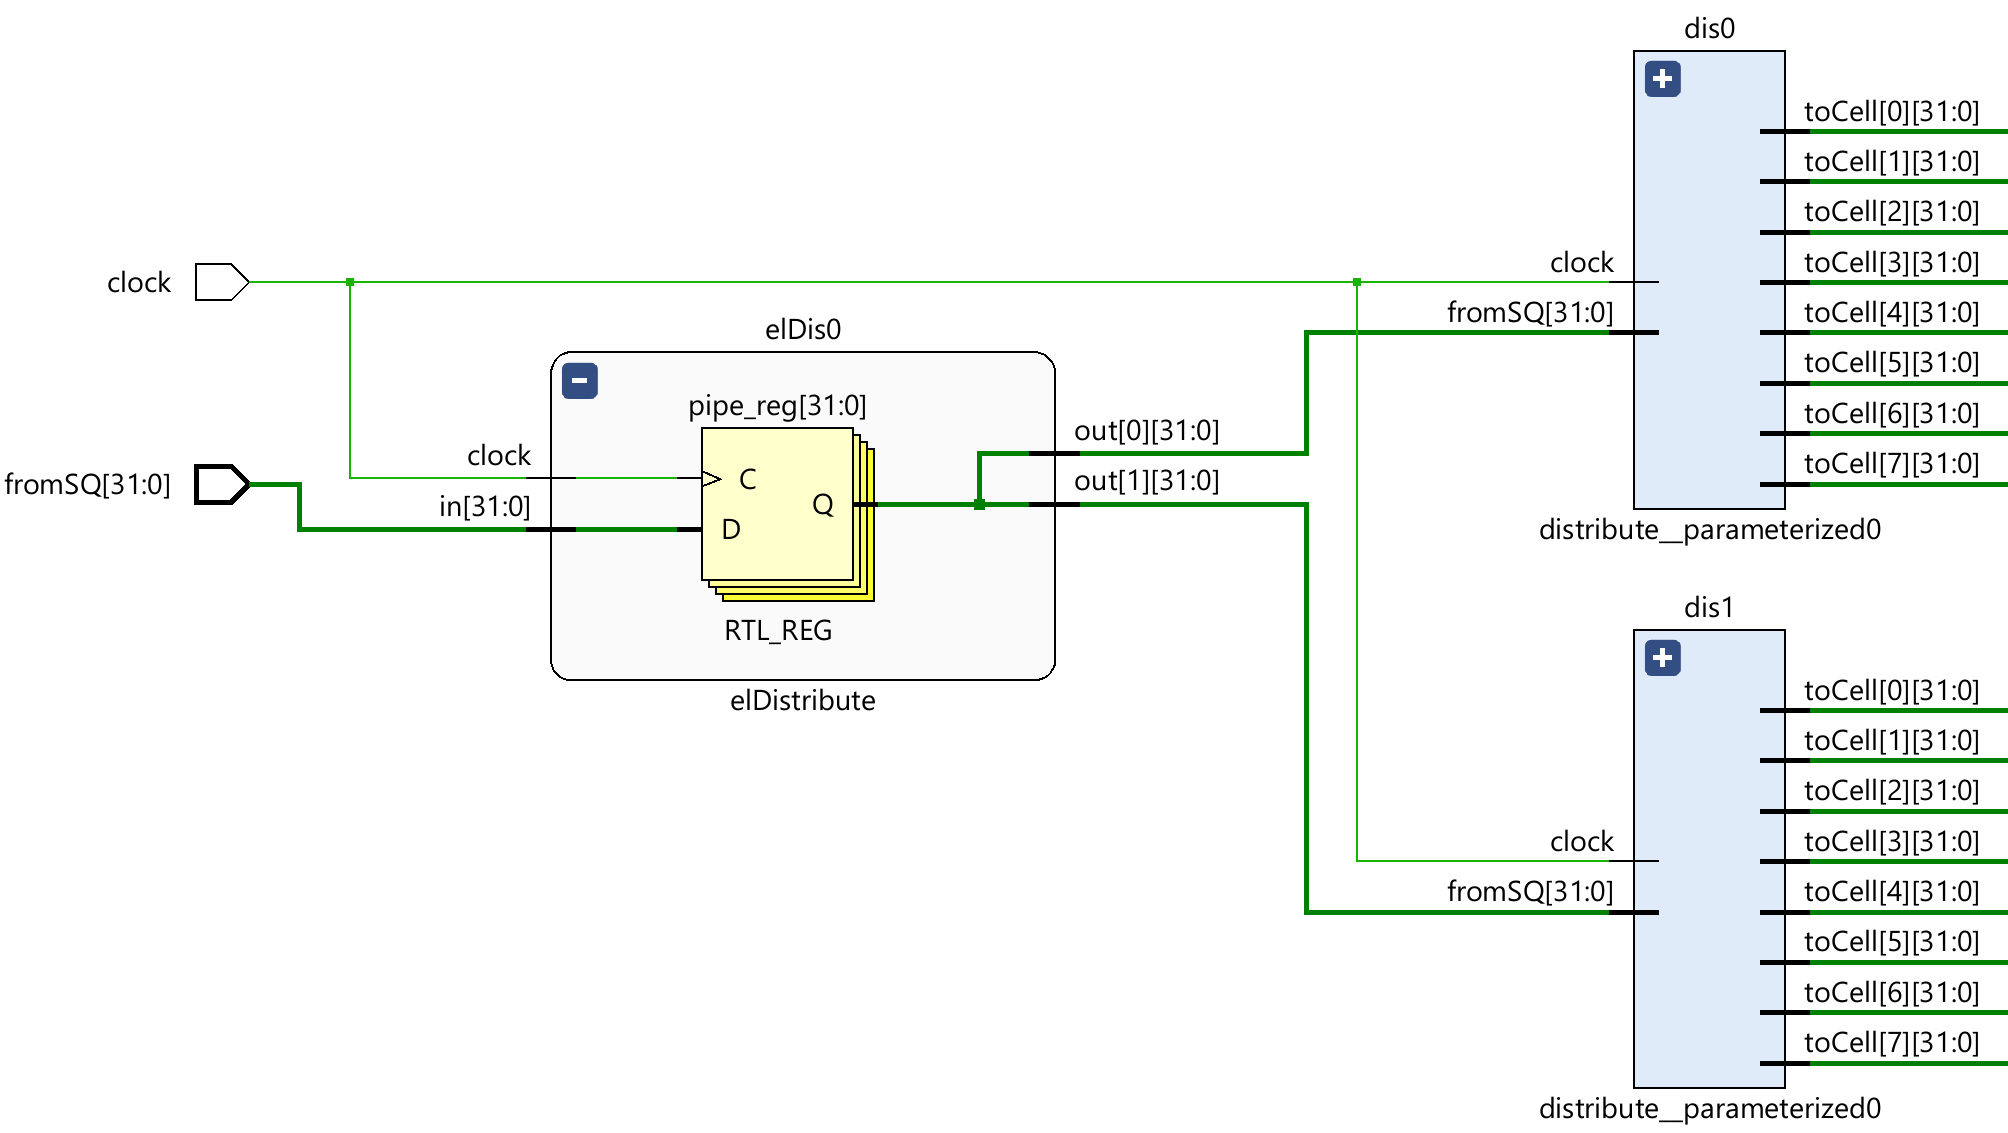
\includegraphics[width=\textwidth]{Images/distribute.png} 
    \caption{The recursively defined distribution network for $p=16$.}
    \label{fig:distribute}
\end{figure}
$\diamond$


\begin{problem}
Design for $p$ and simulate for $p=16$ the reduce network represented in Figure \ref{reduceNet}.

$\diamond$
\end{problem}

\begin{problem}\label{prob:scan}
Let us consider a $p$-input scan network with cells defined on two 34-bit inputs, {\tt in1} and {\tt in2}, and two 34-bit outputs, {\tt out1} and {\tt out2}, synchronized by the clock signal. Design a $p$-input scan network and implement it for $p=16$ in a version independent of the actual content of the cells, i.e., consider only the top level of the design. The pattern of a scan network is exemplified in Figure \ref{fig:scanRedTop} (ignore the output {\tt reduceOut}).

$\diamond$
\end{problem}

\begin{problem}
Redesign the scan network from Problem \ref{prob:scan} emphasizing the reduction output, {\tt reduceOut}, as in representation from Figure \ref{fig:scanRedTop}.

$\diamond$
\end{problem}

%######################
\part{PRACTICAL DESIGNS}
%######################
\chapter{Performance Optimized Digital Logic}\label{chapt:perf_digital_logic}\label{chap:perf_opt_logic}
\localtoc

In previous chapters, we introduced the fundamental principles of zero-order combinational circuits (Chapter \ref{lect1}), first-order memory components, and second-order automata (Chapter \ref{lect3}). While those foundational chapters focused primarily on behavioral and structural correctness, real-world processor architectures demand circuits optimized for high clock frequencies, minimal propagation latency, efficient silicon area, and low power dissipation.

This chapter explores techniques for performance optimization in digital logic. We begin by examining how multiplexing and conditional constructs in hardware description languages synthesize into multiplexer trees versus priority encoders. Next, we analyze high-performance adder topologies that break the sequential carry-propagation bottleneck of simple ripple-carry adders. We then investigate high-performance multiplier architectures---including array multipliers, Radix-4 Modified Booth recoding, Wallace and Dadda carry-save reduction trees, and Redundant Binary Multipliers---that eliminate multiplication latency in compute-intensive execution units. We subsequently examine the microarchitecture of multi-port and multithreaded register files, evaluating the trade-offs between flip-flop arrays, banked SRAMs, and replication. Finally, we analyze sequential timing closure, contrasting Mealy and Moore state machine architectures in high-speed digital pipelines.

\section{Multiplexing and Conditional Logic Optimization in Chisel} \label{sec:muxcase}
\index{multiplexer!optimization}
\index{MuxCase@\texttt{MuxCase}}
\index{when@\texttt{when}}
\index{switch@\texttt{switch}}

In Chisel, designers have several constructs for conditional signal selection and multi-way branching: \texttt{when}, \texttt{switch}, and \texttt{MuxCase} (or \texttt{Mux1H}). The choice among these constructs directly influences the synthesized gate-level netlist, affecting propagation delay, area, and critical path timing.

\subsection{Behavioral and Structural Implications}
The \texttt{when} construct is intuitive for designers accustomed to software-like \texttt{if-else} branching. However, in hardware, nested \texttt{when} statements generate cascaded priority logic, where each condition is evaluated sequentially. Early conditions take precedence, and subsequent conditions are evaluated only if all preceding conditions are false.

In contrast, \texttt{MuxCase} represents priority-free parallel selection logic. When conditions are mutually exclusive, a multiplexer tree is generated where all conditions are evaluated concurrently. This structure often synthesizes into balanced multiplexer trees or parallel Look-Up Table (LUT) structures, resulting in lower latency and superior timing closure.

\subsection{Synthesis Implications}
\textbf{Timing and Performance:}  
For timing, chained \texttt{when} statements introduce a linear increase in propagation delay ($O(N)$ for $N$ conditions) due to the cascading ripple of priority enables. Conversely, \texttt{MuxCase} enables synthesis tools to construct balanced trees ($O(\log N)$ delay), minimizing the critical path when conditions are independent.

\textbf{Area:}  
The \texttt{when} construct can produce compact logic for genuinely prioritized conditions because logic synthesis can prune unused paths early. However, when applied to mutually exclusive cases, priority logic introduces redundant gating. \texttt{MuxCase} directly generates a multiplexer, which maps efficiently to dedicated multiplexer primitives or wide LUTs in modern FPGAs and standard-cell ASIC libraries.

\textbf{Readability and Intent:}  
The \texttt{when} construct clearly conveys priority when priority is inherently required (e.g., interrupt handling or default override). \texttt{MuxCase} is better suited for opcode decoding, instruction selection, and mutually exclusive multi-way branches.

\subsection{Syntax and Implementation Examples}
\textbf{Mutually Exclusive Selection with \texttt{MuxCase}:}  
When conditions are mutually exclusive, \texttt{MuxCase} provides a clean, parallel multiplexer description. The construct takes a default value and a sequence of boolean-condition to data-expression pairs (\texttt{condition -> data}):

\begin{chiselcode}
val result = MuxCase(0.U, Seq(
  (opcode === ADD) -> (a + b),
  (opcode === SUB) -> (a - b)
))
\end{chiselcode}

This description translates directly into a 3-to-1 multiplexer in hardware, selecting between the computed sum, difference, or the default value \texttt{0.U}.

\textbf{Prioritized Selection with \texttt{when}:}  
When conditions require sequential priority, the \texttt{when}/\texttt{elsewhen}/\texttt{otherwise} chain explicitly models this behavior:

\begin{chiselcode}
when(opcode === ADD) {
  result := a + b
}.elsewhen(opcode === SUB) {
  result := a - b
}.otherwise {
  result := 0.U
}
\end{chiselcode}

This logic synthesizes into a chain of multiplexers where the \texttt{ADD} condition controls the final multiplexer stage, imposing priority over the \texttt{SUB} and default cases.

\subsection{Switch Synthesis in Chisel}
In Chisel, the \texttt{switch} construct (available via \texttt{chisel3.util.switch}) provides multi-way branching based on a single selector expression:

\begin{chiselcode}
import chisel3.util._

val result = Wire(UInt(8.W)) 
switch(selector) { 
  is("b00".U) { result := a } 
  is("b01".U) { result := b } 
  is("b10".U) { result := c } 
  is("b11".U) { result := d } 
}
\end{chiselcode}

When the \texttt{is} conditions cover distinct, mutually exclusive literal values of \texttt{selector}, synthesis tools generate a balanced 4-to-1 multiplexer. However, if the selector is wide or conditions overlap, synthesis tools may introduce priority encoders or wide decoders. 

For wide selectors, \texttt{switch} statements can inadvertently create large decoding logic and timing bottlenecks. Furthermore, as noted in Chapter \ref{lect1}, modern Chisel development discourages reliance on \texttt{switch} for complex designs in favor of pattern matching, \texttt{MuxCase}, or \texttt{Mux1H} (one-hot multiplexing), which provide more predictable synthesis results and avoid subtle refactoring bugs.


%*****************************************************************************
\section{High-Performance Adders} \label{sec:high_performance_adders}
%*****************************************************************************
\index{adder!high-performance}
\index{carry lookahead adder (CLA)}
\index{carry select adder (CSelA)}
\index{carry save adder (CSA)}
\index{Kogge-Stone adder}
\index{parallel prefix adder}

In Chapter \ref{lect1}, we analyzed the ripple-carry adder, where the carry out of each bit stage $i$ serves as the carry in to stage $i+1$. Because the carry signal must propagate sequentially through all $N$ full adders, the worst-case critical path delay grows linearly with bit width:
\begin{equation}
t_{\text{RCA}} = t_{\text{gen}} + (N - 1) t_{\text{carry}} + t_{\text{sum}} = O(N)
\end{equation}
For 32-bit and 64-bit ALUs in high-frequency processors, this $O(N)$ latency is unacceptable. High-performance adders employ parallel carry computation, speculative calculation, or carry-deferred representation to reduce arithmetic latency.

\subsection{Carry Lookahead Adder (CLA)}
The Carry Lookahead Adder (CLA) overcomes the carry propagation bottleneck by computing all carry signals in parallel. For each bit position $i$, two intermediate signals are defined:
\begin{align}
\text{Generate: } & G_i = A_i \cdot B_i \\
\text{Propagate: } & P_i = A_i \oplus B_i \quad (\text{or } A_i + B_i)
\end{align}
$G_i$ indicates that a carry is generated at stage $i$ regardless of the carry-in. $P_i$ indicates that an incoming carry $C_i$ will propagate through stage $i$ to $C_{i+1}$.

The carry recurrence relation is:
\begin{equation}
C_{i+1} = G_i + P_i \cdot C_i
\end{equation}
By recursively expanding this relation, each carry bit can be expressed directly in terms of the primary inputs and the initial carry-in $C_0$:
\begin{align}
C_1 &= G_0 + P_0 C_0 \\
C_2 &= G_1 + P_1 G_0 + P_1 P_0 C_0 \\
C_3 &= G_2 + P_2 G_1 + P_2 P_1 G_0 + P_2 P_1 P_0 C_0 \\
C_4 &= G_3 + P_3 G_2 + P_3 P_2 G_1 + P_3 P_2 P_1 G_0 + P_3 P_2 P_1 P_0 C_0
\end{align}
In theory, all carries are available after just two gate delays (an AND level followed by an OR level), enabling constant-time carry computation ($O(1)$). In practice, physical fan-in and fan-out limits restrict flat lookahead blocks to 4 or 8 bits. Larger adders use hierarchical (block) CLA structures, defining block generate ($G_{\text{block}}$) and block propagate ($P_{\text{block}}$) terms, resulting in an overall latency of $O(\log N)$.

\subsection{Carry-Select Adder (CSelA)}
\index{carry select adder (CSelA)}
\index{CSelA@\texttt{CSelA}}
The Carry-Select Adder (CSelA) \cite{bedrij1962} accelerates addition through speculation. The $N$-bit adder is partitioned into smaller blocks (e.g., 4-bit or 8-bit groups). For each block, two additions are performed simultaneously in parallel:
\begin{enumerate}
    \item One adder computes the sum assuming the incoming carry is $0$ ($C_{\text{in}} = 0$).
    \item A second adder computes the sum assuming the incoming carry is $1$ ($C_{\text{in}} = 1$).
\end{enumerate}
When the true carry-in arrives from the preceding block, a 2-to-1 multiplexer selects the precomputed sum and carry-out. 

In a uniform carry-select adder with block size $k$, the carry propagates through $N/k$ multiplexers. To further optimize performance, a \textbf{square-root carry-select adder} uses variable block sizes that increase by one bit per stage (e.g., 2, 3, 4, 5, 6 bits). The larger blocks take progressively longer to compute their tentative sums, but this delay is hidden because the carry-in signal from earlier stages arrives later. This balances the arrival times of data and carry inputs at each multiplexer, achieving an overall delay of:
\begin{equation}
t_{\text{sq-CSelA}} = O(\sqrt{N})
\end{equation}
The Carry-Select Adder provides an effective speed-area trade-off: it reduces delay substantially compared to a ripple-carry adder while avoiding the dense interconnect wiring of a full parallel prefix tree, requiring approximately 40\% to 60\% more area than a ripple-carry adder.

\subsection{Carry-Save Adder (CSA)}
\index{carry save adder (CSA)}
\index{CSA@\texttt{CSA}}
When summing three or more operands (as in multi-operand addition and multiplier partial-product reduction), propagating carries after each addition introduces unnecessary delay. The Carry-Save Adder (CSA) resolves this by deferring carry propagation entirely.

A carry-save adder cell is essentially a Full Adder acting as a \textbf{3:2 compressor}. Given three input bits ($A_i, B_i, C_i$), it produces two output bits: a sum bit $S_i$ and a carry bit $C_{i+1}$:
\begin{align}
S_i &= A_i \oplus B_i \oplus C_i \\
C_{i+1} &= (A_i \cdot B_i) + (B_i \cdot C_i) + (A_i \cdot C_i)
\end{align}
The carry bit $C_{i+1}$ is not forwarded to the adjacent bit cell in the same stage; instead, it is output alongside the sum bit. Thus, adding three $N$-bit numbers produces two $N$-bit results (a partial sum vector and a shifted carry vector) with a delay of only \textit{one full adder} ($O(1)$), completely independent of the operand width $N$.

Carry-save adders are interconnected in tree structures to reduce $K$ partial products down to two vectors in $O(\log_{1.5} K)$ levels of logic, as exemplified by the Wallace tree and Dadda tree networks \cite{wallace1964, dadda1965}. Only in the final stage is a fast two-operand adder (such as a CLA or Kogge-Stone adder) used to merge the carry and sum vectors into a final binary result.

\subsection{Parallel Prefix Adders: Kogge-Stone Adder} \label{sec:kogge-stone-adder}
Parallel prefix adders treat carry computation as a general prefix problem. Binary addition is decomposed into three distinct phases:
\begin{enumerate}
    \item \textbf{Pre-computation}: Generate individual generate and propagate signals for each bit: $g_i = a_i \cdot b_i$, $p_i = a_i \oplus b_i$.
    \item \textbf{Prefix Network}: Combine generate and propagate pairs using the associative \textbf{prefix operator} $\bullet$:
    \begin{equation}
    (G, P) = (g_2, p_2) \bullet (g_1, p_1) = \left( g_2 + (p_2 \cdot g_1), \; p_2 \cdot p_1 \right)
    \end{equation}
    Because the $\bullet$ operator is associative, intermediate terms can be grouped and evaluated in any order, enabling balanced tree networks.
    \item \textbf{Post-computation}: Compute final sum bits using the evaluated carries: $S_i = p_i \oplus C_i$.
\end{enumerate}

The Kogge-Stone Adder is the most prominent parallel prefix topology, optimized for minimum logic depth \cite{kogge1973parallel}. It computes carries in $\lceil \log_2 N \rceil$ stages with a uniform fan-out of 2 at each stage. This makes it one of the fastest adder architectures known for 32-bit, 64-bit, and 128-bit integer units. However, this speed comes at the expense of high wiring density and area: Kogge-Stone requires $O(N \log_2 N)$ prefix operator cells and a large number of routing tracks.

\subsubsection{Comparison of High-Performance Adder Architectures}
Table \ref{tab:adder_comparison} summarizes the asymptotic delay, area, fan-out, and routing complexity of the major adder architectures.

\begin{table}[htbp]
\centering
\small
\setlength{\tabcolsep}{4.5pt}
\begin{tabular}{|l|c|c|c|c|}
\hline
\textbf{Adder Architecture} & \textbf{Logic Delay} & \textbf{Area Complexity} & \textbf{Max Fan-out} & \textbf{Wiring Density} \\ \hline
Ripple-Carry Adder (RCA) & $O(N)$ & $O(N)$ & $O(1)$ & Very Low \\ \hline
Carry Lookahead (CLA) & $O(\log N)$ & $O(N \log N)$ & High & Moderate \\ \hline
Carry-Select (Square-Root, CSelA) & $O(\sqrt{N})$ & $O(N)$ & $O(\sqrt{N})$ & Low \\ \hline
Carry-Save (per stage, CSA) & $O(1)$ & $O(N)$ & $O(1)$ & Low \\ \hline
Kogge-Stone Prefix Adder (KSA) & $O(\log_2 N)$ & $O(N \log_2 N)$ & 2 & Very High \\ \hline
Brent-Kung Prefix Adder (BKA) & $O(2 \log_2 N)$ & $O(N)$ & 2 & Low \\ \hline
\end{tabular}
\caption{Comparison of High-Performance Adder Architectures.}
\label{tab:adder_comparison}
\end{table}

\subsection{Physical ASIC Synthesis of High-Performance Adders on ASAP7 7\,nm FinFET}\label{sec:asap7_adders_synthesis}
\index{adders!ASAP7 7nm FinFET synthesis}\index{synthesis!32-bit adders}\index{carry select adder (CSelA)!delay evaluation}

While asymptotic big-$O$ complexity provides foundational theoretical intuition, real-world arithmetic performance depends on standard-cell driving strengths, interconnect routing congestion, and physical gate delays. To evaluate the practical trade-offs among the adder topologies discussed in this section, five 32-bit adder architectures---Ripple-Carry (RCA), hierarchical Carry Lookahead (CLA), Brent-Kung parallel prefix (BKA) \cite{brent1982regular}, Kogge-Stone parallel prefix (KSA) \cite{kogge1973parallel}, and Carry-Select (CSelA) \cite{bedrij1962}---were implemented in parameterized Chisel RTL, verified with comprehensive functional testbenches covering corner cases, maximum carry propagations, and randomized vectors, and generated into clean gate-level SystemVerilog netlists.

Each design was synthesized using \textbf{Yosys} and mapped with \textbf{Berkeley ABC} to the predictive \textbf{ASAP7 7\,nm FinFET} standard-cell library (\texttt{asap7sc7p5t\_28}, RVT, $V_{dd} = 0.70\,\text{V}$, $T = 25^\circ\text{C}$, Typical TT corner, output capacitive load $C_{\text{load}} = 2.0\,\text{fF}$). Table \ref{tab:asap7_adders_comparison} summarizes the resulting gate counts, standard-cell silicon area, critical path propagation latency, speedup relative to the ripple-carry baseline, and maximum standalone operating clock frequency ($f_{\max} = 1 / t_{\text{pd}}$).

\begin{table}[htbp]
\centering
\footnotesize
\setlength{\tabcolsep}{3.5pt}
\resizebox{\linewidth}{!}{%
\begin{tabular}{|l|c|c|c|c|c|c|}
\hline
\textbf{Adder Architecture} & \textbf{Theoretical} & \textbf{Standard} & \textbf{Total Area} & \textbf{Delay ($t_{\text{pd}}$)} & \textbf{Speedup vs.} & \textbf{Max Frequency} \\
& \textbf{Delay} & \textbf{Cells} & \textbf{($\mu$m$^2$)} & \textbf{(ps / ns)} & \textbf{RCA Baseline} & \textbf{($f_{\max}$, GHz)} \\
\hline
Ripple-Carry Adder (RCA)            & $O(N)$         & 106 & 13.91 & 1,045.43\,ps (1.045\,ns) & $1.00\times$ (Base) & 0.96\,GHz \\
Carry Lookahead Adder (CLA)         & $O(\log N)$    & 122 & 12.98 & 987.99\,ps (0.988\,ns)   & $1.06\times$        & 1.01\,GHz \\
Brent-Kung Prefix Adder (BKA)       & $O(2\log_2 N)$ & 144 & 14.83 & 836.25\,ps (0.836\,ns)   & $1.25\times$        & 1.20\,GHz \\
Kogge-Stone Prefix Adder (KSA)      & $O(\log_2 N)$  & 190 & 17.48 & 712.57\,ps (0.713\,ns)   & $1.47\times$        & 1.40\,GHz \\
\textbf{Carry-Select Adder (CSelA)} & \textbf{$O(\sqrt{N})$} & \textbf{190} & \textbf{18.01} & \textbf{519.83\,ps (0.520\,ns)} & \textbf{2.01$\times$} & \textbf{1.92\,GHz} \\
\hline
\end{tabular}%
}
\caption{Empirical synthesis and timing evaluation of 32-bit high-performance adder architectures mapped to ASAP7 7\,nm FinFET technology.}\label{tab:asap7_adders_comparison}
\end{table}

\subsubsection{Architectural Analysis and Synthesis Insights}
\index{carry select adder (CSelA)!standard cells analysis}
\index{parallel prefix adders!pipelining advantages}

The synthesis results reveal several insights into 7nm arithmetic design:
\begin{enumerate}
    \item \textbf{The Ripple-Carry Bottleneck}: The ripple-carry adder exhibits a propagation delay of $1,045.43\,\text{ps}$ ($1.045\,\text{ns}$). The critical path consists of 31 cascaded majority and inverter stages (\texttt{MAJx2\_ASAP7\_75t\_R}), confirming that the $O(N)$ carry chain is a structural bottleneck in high-frequency datapaths.
    
    \item \textbf{Hierarchical CLA Limitations}: While the 4-bit block CLA reduces delay to $987.99\,\text{ps}$, it offers only a modest $6\%$ speedup. In static CMOS standard cells, the complex multi-input AND-OR trees required for lookahead logic suffer from fan-in stacking and internal node capacitance, diluting the theoretical logarithmic advantage.
    
    \item \textbf{Parallel Prefix Trade-offs}: The parallel prefix trees yield substantial latency reductions: Brent-Kung reaches $836.25\,\text{ps}$ ($1.25\times$ faster) while maintaining a compact $14.83\,\mu\text{m}^2$ footprint. Kogge-Stone further cuts latency to $712.57\,\text{ps}$ ($1.47\times$ faster, $1.40\,\text{GHz}$) by maintaining minimum logic depth ($5$ prefix stages), albeit with higher cell count (190 cells) and dense inter-stage routing tracks.
    
    \item \textbf{Carry-Select Characteristics}: In this 32-bit standard-cell evaluation, the Carry-Select Adder (CSelA) achieves the lowest propagation delay: 519.83\,ps (0.520\,ns), delivering a $2.01\times$ speedup over the ripple-carry baseline and reaching a standalone frequency of 1.92\,GHz.
    
    In 32-bit standard cells, partitioning the adder into 4-bit blocks allows the speculative carry chains to settle in parallel in under $120\,\text{ps}$. The arriving carries then ripple through a linear chain of transmission-gate and static multiplexers (\texttt{NAND2}, \texttt{MAJI}), each introducing an average gate delay of only $\approx 35\text{--}40\,\text{ps}$. Because 2:1 multiplexers are among the fastest and most highly optimized primitives in modern FinFET standard-cell libraries, the carry-select topology performs exceptionally well at the 32-bit operand width.
    
    \item \textbf{Technology and Scaling Trade-Offs in the Literature}: While the Carry-Select Adder exhibits favorable delay at 32 bits in this static CMOS library, published research in computer arithmetic demonstrates that its relative performance depends heavily on operand width, technology node, and pipeline partitioning:
    \begin{itemize}
        \item \textit{Scaling to 64-bit and 128-bit Datapaths}: As analyzed by Knowles \cite{knowles2001} and Harris \cite{harris2003taxonomy}, Carry-Select adder delay scales with $O(\sqrt{N})$, whereas parallel prefix adders scale with $O(\log_2 N)$. For 64-bit and 128-bit words, the logarithmic depth of prefix networks (such as Kogge-Stone, Han-Carlson \cite{han1987}, or Knowles networks) yields lower propagation latency than carry-select schemes, whose rippling multiplexer chains become the dominant delay path.
        \item \textit{Ease of Pipelining}: Parallel prefix adders feature regular, feed-forward directed acyclic graph topologies with uniform logic depth across all bit positions. This structural regularity makes prefix adders straightforward to pipeline across multiple clock cycles by inserting pipeline registers between prefix levels (e.g., two prefix levels per cycle). In contrast, pipelining a Carry-Select Adder requires retiming the multiplexer chain across speculative block boundaries, which introduces irregular pipeline cuts, uneven stage delays, and significant register overhead.
        \item \textit{Interconnect and Driving Strength Variations}: In technologies with high interconnect resistance or standard-cell libraries lacking transmission-gate multiplexers, parallel prefix adders and hybrid prefix/carry-select topologies (such as Han-Carlson adders \cite{han1987}) often achieve better timing closure and lower power dissipation than pure carry-select designs \cite{beaumont2001}.
    \end{itemize}
\end{enumerate}


%*****************************************************************************
\section{High-Performance Multipliers} \label{sec:high_performance_multipliers}
%*****************************************************************************
\index{multiplier!high-performance}
\index{array multiplier}
\index{Booth multiplier!Radix-4}
\index{Wallace tree multiplier}
\index{Dadda tree multiplier}
\index{redundant binary multiplier (RBM)}
\index{redundant binary signed-digit (RBSD)}
\index{DSP!multiplier microarchitecture}

In modern microprocessor and digital signal processor (DSP) execution units, multiplication is one of the most performance-critical and hardware-intensive operations. While an $N$-bit addition requires combining two operands, an $N \times N$-bit multiplication fundamentally computes the sum of $N$ shifted partial products, yielding a $2N$-bit product.

Hardware multiplication decomposes into three distinct microarchitectural phases:
\begin{enumerate}
    \item \textbf{Partial Product Generation (PPG)}: Generating the individual partial product vectors $P_i = A \cdot B_i \cdot 2^i$ from multiplicand $A$ and multiplier bits $B_i$.
    \item \textbf{Partial Product Reduction (PPR)}: Compressing the $N$ partial product vectors into two equivalent vectors (typically sum and carry vectors) using parallel carry-save arithmetic.
    \item \textbf{Final Carry-Propagate Addition (CPA)}: Adding the final sum and carry vectors using a high-speed adder (such as a Carry Select or parallel prefix adder) to produce the standard binary product.
\end{enumerate}

The critical path and silicon area of a multiplier are overwhelmingly dominated by Phase 2 (the reduction network). Consequently, computer architects have devised specialized reduction topologies to accelerate multiplication.

\subsection{Array Multipliers}
\index{array multiplier!carry-save array}

The \textit{Array Multiplier} implements a direct two-dimensional spatial mapping of pencil-and-paper multiplication. For an $N \times N$ multiplier, an $N \times N$ matrix of AND gates generates the elementary bit-products $a_j \cdot b_i$. 

In a linear carry-save array, each row of full adders accumulates one partial product row into the running accumulated sum and carry vectors. The carries generated in row $i$ do not ripple horizontally; instead, they are passed diagonally downward to row $i+1$, while the sums are passed vertically downward. Carry propagation occurs only in the final row via a vector-merging adder.

\textbf{Complexity and Trade-offs}:
\begin{itemize}
    \item \textit{Delay}: The critical path traverses $N$ adder cells vertically through the array, plus the final $N$-bit ripple carry propagation:
    \begin{equation}
    t_{\text{Array}} = (N - 1) t_{\text{carry}} + t_{\text{CPA}} = O(N).
    \end{equation}
    
    \item \textit{Area}: The array requires $N^2$ AND gates and approximately $N(N - 1)$ full adders:
    \begin{equation}
    A_{\text{Array}} = O(N^2).
    \end{equation}
    
    \item \textit{Physical Layout}: The primary advantage of the array multiplier is its strictly planar, regular 2D systolic topology. Cells are interconnected exclusively via short, nearest-neighbor routing channels, ensuring uniform interconnect wire delays and minimal parasitic capacitance. However, for word widths $N \ge 32$, its $O(N)$ propagation latency creates a clock frequency bottleneck.
\end{itemize}

\subsection{Radix-4 Modified Booth Recoding}
\index{Booth multiplier!Radix-4 recoding}
\index{Booth recoding!modified}

Rather than generating $N$ separate partial products, \textit{Radix-4 Modified Booth Recoding} \cite{booth1951, macsorley1961} inspects three consecutive multiplier bits with a 1-bit overlap $(b_{2i+1}, b_{2i}, b_{2i-1})$ to recode the multiplier into a signed-digit base-4 representation with digit set $d_i \in \{-2, -1, 0, +1, +2\}$:
\begin{equation}
d_i = -2 b_{2i+1} + b_{2i} + b_{2i-1}.
\end{equation}
Table \ref{tab:booth_radix4} summarizes the Radix-4 recoding rules.

\begin{table}[htbp]
\centering
\small
\begin{tabular}{|ccc|c|c|l|}
\hline
$b_{2i+1}$ & $b_{2i}$ & $b_{2i-1}$ & Recoded Digit ($d_i$) & Partial Product ($PP_i$) & Hardware Operation \\
\hline
0 & 0 & 0 &  $0$ &  $0$          & String of zeros \\
0 & 0 & 1 & $+1$ & $+A$          & Multiplicand $A$ \\
0 & 1 & 0 & $+1$ & $+A$          & Multiplicand $A$ \\
0 & 1 & 1 & $+2$ & $+2A$         & 1-bit arithmetic left shift ($A \ll 1$) \\
1 & 0 & 0 & $-2$ & $-2A$         & Bitwise inversion of $2A$, carry-in $+1$ \\
1 & 0 & 1 & $-1$ & $-A$          & Bitwise inversion of $A$, carry-in $+1$ \\
1 & 1 & 0 & $-1$ & $-A$          & Bitwise inversion of $A$, carry-in $+1$ \\
1 & 1 & 1 &  $0$ &  $0$          & String of zeros \\
\hline
\end{tabular}
\caption{Radix-4 Modified Booth Recoding Truth Table.}
\label{tab:booth_radix4}
\end{table}

\textbf{Architectural Impact}:
\begin{enumerate}
    \item \textit{50\% Reduction in Partial Products}: By grouping multiplier bits in pairs, the number of partial product rows is halved from $N$ to $\lceil (N + 1) / 2 \rceil$. For a 32-bit multiplier, only 17 partial products are generated instead of 32.
    
    \item \textit{Trivial Multiple Generation}: The multiple $\pm 2A$ requires only a simple 1-bit hardwired left shift, avoiding any carry-propagate precomputations (unlike Radix-8 Booth recoding, which requires generating $3A = 2A + A$).
    
    \item \textit{Signed and Unsigned Support}: Both signed and unsigned operations are handled by extending the sign bit or zero-padding the upper bit positions.
\end{enumerate}
By halving the number of operands entering the reduction tree, Radix-4 Booth recoding eliminates almost half of the reduction logic, reducing both silicon area and reduction tree depth.

\subsection{Carry-Save Reduction Trees: Wallace and Dadda Trees}
\index{Wallace tree multiplier}
\index{Dadda tree multiplier}
\index{carry-save adder (CSA)!tree reduction}

Once partial products are generated, they must be compressed into two equivalent vectors. In an unpipelined linear array, partial products are accumulated serially. \textit{Tree multipliers} compress partial products in parallel across both dimensions using Carry-Save Adders (CSAs). A 3:2 full adder compresses three binary inputs into two outputs (sum and carry) in $O(1)$ gate delays, while a 2:2 half adder compresses two inputs into two outputs.

\subsubsection{Wallace Trees}
In a \textit{Wallace Tree} \cite{wallace1964}, full adders and half adders are deployed greedily at every level of the reduction hierarchy. In each reduction stage:
\begin{itemize}
    \item Every available group of three bits at column $j$ is routed to a 3:2 counter.
    \item Every remaining pair of two bits is routed to a 2:2 counter.
    \item Any solitary single bit is passed directly to the next stage.
\end{itemize}
Because each stage reduces the number of rows by a factor of approximately $3/2 = 1.5$, the height of the partial product matrix decreases exponentially:
\begin{equation}
h_{k+1} = 2 \lfloor h_k / 3 \rfloor + (h_k \bmod 3).
\end{equation}
The number of reduction levels required to compress $N$ partial products down to 2 rows is logarithmic:
\begin{equation}
L_{\text{Wallace}} = \lceil \log_{1.5} (N / 2) \rceil = O(\log N).
\end{equation}
For $N = 32$ rows, a Wallace tree requires only 8 reduction levels; combined with Radix-4 Booth recoding (17 rows), the tree depth collapses to just 6 levels.

\subsubsection{Dadda Trees}
A \textit{Dadda Tree} \cite{dadda1965} optimizes the Wallace construction by deferring compression. Rather than reducing as aggressively as possible in early stages, Luigi Dadda showed that the number of reduction stages is identical if compression is delayed to match the maximum capacity of each subsequent stage (the sequence $d_1 = 2, d_2 = 3, d_3 = 4, d_4 = 6, d_6 = 9, d_7 = 13, d_8 = 19, \dots$, where $d_{j+1} = \lfloor 1.5 d_j \rfloor$).

By placing full and half adders only when the number of bits in a column exceeds the target threshold $d_j$, Dadda multipliers use fewer counters in early stages than Wallace trees. However, this leaves more uncompressed bits at the boundary, requiring a slightly wider final Carry-Propagate Adder.

\subsubsection{Physical Design Challenge: Interconnect Congestion}
Despite their asymptotic speed ($O(\log N)$ delay), Wallace and Dadda trees present significant physical design hurdles in modern deep-submicron and FinFET ASIC processes:
\begin{itemize}
    \item \textit{Irregular Wiring Topology}: Connections between compression stages do not follow regular nearest-neighbor grids. Signals in high-order columns must be routed across large distances to distant full adders.
    \item \textit{Interconnect Congestion}: The complex tree topology creates dense routing congestion in standard-cell place-and-route tools, consuming multiple metal layers and increasing parasitic coupling capacitance.
    \item \textit{Non-uniform Wire Delays}: Because wire lengths vary drastically across the tree, interconnect RC delays can degrade or even negate the theoretical gate-level latency advantage over regular structures.
\end{itemize}

\subsection{Redundant Binary Multiplier (RBM)}
\index{redundant binary multiplier (RBM)}
\index{redundant binary adder (RBA)}
\index{redundant binary signed-digit (RBSD)}
\index{carry-free addition}

To overcome the irregular routing congestion of Wallace trees while maintaining logarithmic delay, computer architects developed the \textit{Redundant Binary Multiplier (RBM)}. The RBM is grounded in the Redundant Binary Signed-Digit (RBSD) arithmetic originally formulated by Avizienis \cite{avizienis1961} and adapted for VLSI by Takagi, Yasuura, and Yajima \cite{takagi1985}.

\subsubsection{Redundant Binary Representation}
In a radix-2 redundant binary system, each digit $x_i$ takes values from the signed-digit set:
\begin{equation}
x_i \in \{-1, 0, 1\} \quad (\text{denoted } \{\bar{1}, 0, 1\}).
\end{equation}
In hardware, each redundant binary digit is encoded using two binary bits $(x_i^+, x_i^-)$ such that its numerical value is:
\begin{equation}
x_i = x_i^+ - x_i^-.
\end{equation}
A digit $x_i = 1$ is encoded as $(1, 0)$, $x_i = -1$ as $(0, 1)$, and $x_i = 0$ as $(0, 0)$ (or $(1, 1)$).

\subsubsection{Constant-Time Carry-Free Addition}
The advantage of the redundant binary number system is that two redundant binary numbers can be added in strictly $O(1)$ constant time without any carry propagation, regardless of word length.

In a standard binary adder, the carry at position $i$ can propagate across all higher bit positions because a carry generate at position 0 can ripple through an unbroken chain of propagate conditions ($P_i = 1$). In contrast, an $N$-bit Redundant Binary Adder (RBA) eliminates this chain entirely by exploiting redundancy: when an intermediate carry must be generated, the cell speculatively selects its intermediate sum and carry such that no incoming carry from the adjacent lower position can cause a secondary carry overflow.

Specifically, at digit position $i$, an RBA cell receives $x_i, y_i \in \{-1, 0, 1\}$. Their sum $T_i = x_i + y_i \in \{-2, -1, 0, 1, 2\}$ is decomposed into an intermediate carry $c_{i+1} \in \{-1, 0, 1\}$ and intermediate sum $s_i \in \{-1, 0, 1\}$:
\begin{equation}
2 c_{i+1} + s_i = x_i + y_i.
\end{equation}
To ensure that the final digit $z_i = s_i + c_i \in \{-1, 0, 1\}$ never exceeds $+1$ or $-1$, the RBA cell inspects the polarity of the adjacent lower operand digits $p_{i-1} = (x_{i-1} + y_{i-1} > 0)$:
\begin{itemize}
    \item When $T_i = 1$: If $p_{i-1}$ indicates that incoming carry $c_i$ could be positive ($c_i \ge 0$), the cell chooses $c_{i+1} = 1$ and $s_i = -1$. Because $s_i = -1$, the arrival of $c_i = 1$ produces $z_i = -1 + 1 = 0 \le 1$. If $p_{i-1}$ indicates $c_i \le 0$, the cell chooses $c_{i+1} = 0$ and $s_i = 1$.
    \item When $T_i = -1$: If $p_{i-1}$ indicates $c_i \ge 0$, the cell chooses $c_{i+1} = 0$ and $s_i = -1$. If $c_i \le 0$, it chooses $c_{i+1} = -1$ and $s_i = 1$.
    \item When $T_i = \pm 2$: $c_{i+1} = \pm 1$ and $s_i = 0$.
    \item When $T_i = 0$: $c_{i+1} = 0$ and $s_i = 0$.
\end{itemize}
Because intermediate carry $c_{i+1}$ depends \textit{only} on the local operands $(x_i, y_i)$ and the adjacent lower operands $(x_{i-1}, y_{i-1})$, carry propagation terminates after exactly one bit position. The delay of an RBA cell is strictly constant:
\begin{equation}
t_{\text{RBA}} = O(1).
\end{equation}

\subsubsection{Balanced Binary Reduction Tree}
Because each RBA cell adds two redundant binary vectors into a single redundant binary vector ($2 \to 1$ reduction), an RBM arranges its partial product reduction as a strictly balanced binary tree rather than the irregular $3:2$ grouping of Wallace trees:
\begin{itemize}
    \item \textit{Tree Structure}: In a 32-bit multiplier, 32 partial products are initially grouped into 16 redundant binary pairs.
    
    \item \textit{Binary Tree Depth}: At each tree level $k$, the number of vectors is exactly halved: $16 \to 8 \to 4 \to 2 \to 1$. The tree depth is strictly:
    \begin{equation}
    D_{\text{RBM}} = \lceil \log_2 N \rceil.
    \end{equation}
    For $N = 32$, exactly $\log_2(32) = 5$ RBA levels reduce all 32 partial products down to a single redundant binary result $(P^+, P^-)$.
    
    \item \textit{Final RB-to-Binary Conversion}: At the root of the tree, the single redundant binary number is converted to standard two's complement binary via a high-speed subtractor:
    \begin{equation}
    P = P^+ - P^-.
    \end{equation}
    This final conversion is computed in parallel using a Carry-Select (CSelA) or parallel prefix adder.
\end{itemize}


In high-performance microprocessors and custom arithmetic datapaths, designers widely employ Radix-4 Modified Booth recoding combined with balanced 4:2 carry-save compressor trees \cite{santoro1989, goto1992, ohkubo1995}. This combination provides a regular layout and halves the number of partial products, avoiding both the irregular routing of Wallace trees and the area and dual-rail wiring overhead of redundant binary logic.

\subsection{Architectural Comparison of High-Performance Multipliers}

Table \ref{tab:multiplier_comparison} summarizes the structural, asymptotic, and physical layout characteristics of the major multiplier architectures.

\begin{table}[htbp]
\centering
\footnotesize
\setlength{\tabcolsep}{3pt}
\resizebox{\linewidth}{!}{%
\begin{tabular}{|l|c|c|c|c|p{4.2cm}|}
\hline
\textbf{Architecture} & \textbf{Delay Complexity} & \textbf{Area Complexity} & \textbf{Reduction Structure} & \textbf{Routing Regularity} & \textbf{Typical Application Domain} \\
\hline
Array Multiplier        & $O(N)$                 & $O(N^2)$                 & Linear 1D cascade         & High (Planar 2D)            & Low-frequency, small bit-widths ($N \le 16$) \\
Radix-4 Booth           & $O(N)$ or $O(\log N)$  & $O(N^2)$ / $O(N \log N)$ & Halved rows (17 for 32b)  & High (Booth recoder)        & Standard-cell ASICs, area-constrained cores \\
Wallace Tree Multiplier & $O(\log_{1.5} N)$      & $O(N^2)$                 & Irregular 3:2 CSA tree     & Low (Wiring congestion)     & High-speed arithmetic units \\
Dadda Tree Multiplier   & $O(\log_{1.5} N)$      & $O(N^2)$                 & Deferral 3:2 CSA tree      & Low (Wiring congestion)     & Minimum counter count in standard cells \\
Redundant Binary (RBM)  & $O(\log_2 N)$          & $O(N^2)$                 & Balanced 2:1 binary tree   & High (Modular H-Tree)       & Custom VLSI DSPs \\
\hline
\end{tabular}%
}
\caption{Architectural Comparison of High-Performance Multiplier Topologies.}
\label{tab:multiplier_comparison}
\end{table}

While big-$O$ asymptotic analysis provides valuable theoretical insight, real-world processor performance is determined by standard-cell library characteristics, FinFET gate drive strengths, and physical wiring parasitics.

\subsection{Automated Standard-Cell Synthesis vs. Custom Datapath Implementation}\label{sec:multiplier_eda_synthesis_realities}\label{riscvMultiplierSynthesis}
\index{multiplier!synthesis realities}
\index{multiplier!ASAP7 7nm FinFET synthesis}
\index{synthesis!Yosys multiplier inference}
\index{synthesis!Berkeley ABC optimization}
\index{Booth multiplier!front-end delay penalty}
\index{redundant binary multiplier!custom DSP layout}
\index{redundant binary arithmetic}

While big-$O$ asymptotic complexity analysis provides fundamental theoretical guidance, real-world microprocessor execution unit performance is governed by standard-cell library electrical characteristics, FinFET gate drive strengths, automated logic synthesis algorithms, and deep-submicron wiring parasitics. 

In commercial high-performance microprocessors and digital signal processors, execution unit multipliers are rarely implemented via unguided standard-cell logic synthesis. Instead, processor architects typically employ one of two methodologies:
\begin{enumerate}
    \item \textit{Commercial Datapath Synthesis}: EDA environments like Synopsys Design Compiler (with DesignWare) or Cadence Genus (with ChipWare) provide specialized, configurable arithmetic generator blocks. These tools recognize arithmetic operations and map them directly into parameter-tuned 4:2 compressor trees, Radix-4 or Radix-8 Booth recoders, and parallel-prefix final adders optimized for user timing constraints.
    
    \item \textit{Custom Datapath Macro Design}: In high-frequency commercial processors (documented extensively in IEEE ISSCC, JSSC, and CICC literature \cite{santoro1989, goto1992, ohkubo1995, goto1997, hagihara1998}), multipliers are hand-crafted as hardened, pitch-matched datapath macros. Designers use optimized custom dynamic/static compound gates, transmission-gate multiplexers, and dedicated metal routing channels to eliminate interconnect congestion and achieve single-digit gigahertz clock frequencies. In custom silicon, tree multipliers and Booth recoders run significantly faster than array multipliers ($O(\log N)$ vs. $O(N)$) because custom physical layout avoids the placement scattering and wire congestion of standard cells.
\end{enumerate}

To evaluate how standard-cell logic synthesis behaves when unguided by commercial macro generators, each 32-bit multiplier architecture was modeled in parameterized Chisel RTL, verified against randomized signed and unsigned testbenches, generated into clean gate-level SystemVerilog, and synthesized using the open-source Yosys framework and Berkeley ABC targeting the predictive ASAP7 7\,nm FinFET standard-cell library (\texttt{asap7sc7p5t\_28}, RVT, $V_{dd} = 0.70\,\text{V}$, $T = 25^\circ\text{C}$, Typical TT corner, output capacitive load $C_{\text{load}} = 2.0\,\text{fF}$).

Table \ref{tab:ch15_asap7_multipliers} presents the empirical physical synthesis results for all five 32-bit multiplier configurations.

\begin{table}[htbp]
\centering
\footnotesize
\setlength{\tabcolsep}{3.5pt}
\resizebox{\linewidth}{!}{%
\begin{tabular}{|l|c|c|c|c|c|c|}
\hline
\textbf{Multiplier Architecture} & \textbf{Standard Cells} & \textbf{Area ($\mu$m$^2$)} & \textbf{Delay ($t_{\text{pd}}$)} & \textbf{Standalone $f_{\max}$} & \textbf{Area vs. Base} & \textbf{Speedup} \\
\hline
Behavioral Multiplier (Baseline) & 10,240 & 1,083.36 & 2,148.00\,ps (2.148\,ns) & 0.466\,GHz & Baseline & $1.00\times$ \\
Array Multiplier                 & 5,405  & 527.04   & \textbf{1,967.86\,ps (1.968\,ns)} & \textbf{0.508\,GHz} & $-51.4\%$ & $\mathbf{1.09\times}$ \\
Radix-4 Modified Booth           & 5,590  & \textbf{464.45} & 2,159.88\,ps (2.160\,ns) & 0.463\,GHz & $\mathbf{-57.1\%}$ & $0.99\times$ \\
Wallace Tree Multiplier          & 7,293  & 627.77   & 2,088.55\,ps (2.089\,ns) & 0.479\,GHz & $-42.0\%$ & $1.03\times$ \\
Redundant Binary Multiplier (RBM)& 14,920 & 1,072.65 & 2,245.91\,ps (2.246\,ns) & 0.445\,GHz & $-1.0\%$  & $0.96\times$ \\
\hline
\end{tabular}%
}
\caption{Empirical synthesis and timing evaluation of 32-bit multiplier architectures mapped to ASAP7 7\,nm FinFET predictive standard-cell library ($V_{dd} = 0.70\,\text{V}$, $C_{\text{load}} = 2.0\,\text{fF}$).}\label{tab:ch15_asap7_multipliers}
\end{table}


\subsubsection{Yosys Multiplier Synthesis}
\index{Yosys!alumacc pass}\index{Yosys!maccmap pass}\index{Berkeley ABC!AIG rewriting}\index{Brent-Kung adder!synthesis baseline}

When a hardware designer writes a multiplication expression in HDL (such as \texttt{val product = io.a * io.b} in Chisel or \texttt{assign p = a * b} in Verilog), modern logic synthesizers do not implement a naive shift-and-add algorithm or a sequential state machine. In open-source synthesis flows like Yosys:
\begin{itemize}
    \item \textit{AST Cell Extraction}: The HDL elaboration phase infers an abstract internal multiplication operator cell (\texttt{\$mul}).
    
    \item \textit{Multiply-Accumulate Transformation (\texttt{alumacc})}: The synthesis engine executes the \texttt{alumacc} pass, scanning the design hierarchy to group multiplication, addition, and subtraction operations into multi-operand multiply-accumulate macro-cells (\texttt{\$macc}).
    
    \item \textit{Carry-Save Compressor Tree Mapping (\texttt{maccmap})}: Rather than flattening the multiplication into a linear ripple-carry chain, the \texttt{maccmap} pass expands the \texttt{\$macc} cell into a bit-slice carry-save compressor tree built from 1-bit full adders (\texttt{\$fa}). In Yosys technology mapping, the carry-lookahead cell (\texttt{\$lcu}) is mapped by default to a Brent-Kung parallel-prefix carry tree (\texttt{\_90\_lcu\_brent\_kung}) to merge the final sum and carry vectors.
    
    \item \textit{Boolean Resynthesis and Delay Optimization (Berkeley ABC)}: The resulting netlist is processed by Berkeley ABC for technology mapping. ABC executes structural hashing (\texttt{strash}), Functional Redundancy Identification, and cut-based delay mapping (\texttt{dch}, \texttt{map}) targeting the ASAP7 standard-cell library. ABC restructures logic cones along the critical path into balanced And-Inverter Graph (AIG) trees.
\end{itemize}

Consequently, the synthesizer's ``behavioral baseline'' is already an optimized carry-save compressor tree with a parallel-prefix final adder. 

In the RISC-V \texttt{Zmmul} extension, the datapath must support four distinct signed/unsigned multiplication instructions: \texttt{MUL}, \texttt{MULH}, \texttt{MULHSU}, and \texttt{MULHU}. In behavioral HDL code, a common implementation writes separate multiplication expressions under a conditional multiplexer:

\begin{chiselcode}
when(io.isSigned === 1.U) {
  io.result := (io.a.asSInt * io.b.asSInt).asUInt
}.otherwise {
  io.result := io.a * io.b
}
\end{chiselcode}

Because Chisel emits Verilog with separate signed and unsigned multiplication operators (\texttt{\$signed(a) * \$signed(b)} versus \texttt{a * b}), the synthesis front-end assigns distinct signedness attributes to each operator. As a result, the synthesizer instantiates two complete, independent 64-bit carry-save compressor trees behind an output multiplexer---one for sign-extended signed operands and one for zero-extended unsigned operands. This duplication doubled the cell count and silicon area without improving propagation delay.

To prevent this duplication, the designer can condition the inputs before multiplication rather than multiplexing the outputs of two separate multiplier trees. By extending both 32-bit operands by one bit to 33 bits and conditionally setting the sign bit based on the operation, a single signed $33 \times 33$ multiplier computes all signed, unsigned, and mixed-signed combinations:

\begin{chiselcode}
val isSignedA = (io.mulOp === AluOp.MULH) || (io.mulOp === AluOp.MULHSU)
val isSignedB = (io.mulOp === AluOp.MULH)

val aExt = Cat(Mux(isSignedA, io.a(31), 0.U(1.W)), io.a).asSInt
val bExt = Cat(Mux(isSignedB, io.b(31), 0.U(1.W)), io.b).asSInt
val product = (aExt * bExt).asUInt

val result = Mux(io.isHigh, product(63, 32), product(31, 0))
\end{chiselcode}

By conditioning the operands prior to multiplication, only a single multiplication AST node is generated in the emitted hardware description. This cuts the synthesized compressor tree area and cell count in half while preserving single-cycle throughput, a technique we employ in our pipelined multiplier design.

\subsubsection{Array Multiplier Standard Cell Synthesis}
\index{array multiplier!synthesis delay advantage}\index{partial product generation!AND gate delay}

The Array Multiplier achieved the lowest propagation delay of all evaluated topologies under Yosys/ABC: 1,967.86\,ps (1.968\,ns), operating at 0.508\,GHz ($1.09\times$ speedup over the baseline). This result may appear counterintuitive because textbook array multipliers have an asymptotic delay complexity of $O(N)$. 

The explanation lies in the front-end timing of Phase 1 (Partial Product Generation) and the behavior of the logic synthesizer:
\begin{enumerate}
    \item \textit{Instantaneous Partial Product Generation}: In the array multiplier, every single bit-product $P_{i,j} = A_j \cdot B_i$ is computed by an independent 2-input \texttt{AND2} gate. In the ASAP7 7\,nm FinFET technology library, an \texttt{AND2x2\_ASAP7\_75t\_R} cell has an intrinsic propagation delay of  \textbf{$\approx 15\,\text{ps}$}. There is zero decoding logic, zero multiplexing, and zero operand negation. All 1,024 partial product bits are available almost simultaneously at $t \approx 15\,\text{ps}$.
    
    \item \textit{Multi-Operand Synthesis Optimization}: When the partial product summation is expressed as a multi-operand sum ($\sum_{i=0}^{31} T_i$), Yosys and ABC do not lay out the full adders as a single-rail linear cascade. Instead, the synthesizer decomposes the 32 input terms into a balanced tree of carry-save adders, and ABC's cut-based delay mapping restructures the logic into a shallow AIG tree.
    
    \item \textit{Absence of Front-End Overhead}: Because the array multiplier begins reduction with zero front-end logic penalty, the entire budget of the clock period is dedicated to reduction and vector merging. In an unpipelined 32-bit datapath, this clean front-end allows the netlist to reach the final vector-merging adder earlier than architectures burdened by complex recoding logic.
\end{enumerate}

However, this delay advantage is specific to unguided automated standard-cell synthesis at 32 bits. In custom VLSI silicon or deep-submicron layouts with physical wire routing constraints, the linear $O(N)$ carry ripple and large cell count make array multipliers unsuitable for high-frequency processors compared to custom tree multipliers \cite{santoro1989}.

\subsubsection{Radix-4 Booth Recoding Standard Cell Synthesis}
\index{Booth multiplier!front-end penalty}\index{Booth multiplier!area reduction}\index{Radix-4!breakeven analysis}

The Radix-4 Modified Booth Multiplier achieved an area of 464.45\,$\mu$m$^2$ (5,590 cells) and a critical path delay of 2,159.88\,ps (2.160\,ns). While it achieved a 57.1\% reduction in silicon area compared to the baseline (and 12\% less area than the Array Multiplier), its propagation delay was slightly higher than that of the Array Multiplier ($2.160\,\text{ns}$ vs. $1.968\,\text{ns}$).

This outcome illustrates a fundamental architectural trade-off between front-end recoding overhead and reduction tree depth:
\begin{itemize}
    \item \textit{Reduction Tree Savings}: Radix-4 Booth recoding inspects overlapping 3-bit windows of the multiplier, reducing the number of partial product rows from 32 down to 17 ($N/2 + 1$). In a carry-save reduction tree, reducing the number of operands from 32 to 17 eliminates approximately two levels of carry-save compressors:
    \begin{equation}
    \Delta D_{\text{tree}} \approx \lceil \log_{1.5}(32) \rceil - \lceil \log_{1.5}(17) \rceil \approx 8 - 6 = 2 \text{ levels}.
    \end{equation}
    In ASAP7 7\,nm FinFET, each 3:2 carry-save adder level introduces approximately $40\,\text{ps}$ of logic delay. Therefore, eliminating two reduction levels saves roughly:
    \begin{equation}
    \Delta t_{\text{reduction}} \approx 2 \times 40\,\text{ps} = 80\,\text{ps}.
    \end{equation}
    
    \item \textit{Front-End Recoding Penalty}: Unlike the Array Multiplier's single-gate AND generation ($\approx 15\,\text{ps}$), generating a Radix-4 Booth partial product requires:
    \begin{enumerate}
        \item Booth window decoding logic to compute the control signals $\{ \text{zero}, \text{one}, \text{two}, \text{negate} \}$;
        \item A 5:1 multiplexer per bit position to select among $0, +A, +2A, -A,$ and $-2A$;
        \item Inversion and carry-in generation logic ($\sim A + 1$) to compute two's complement negations.
    \end{enumerate}
    In ASAP7 standard cells, this front-end decoding, multiplexing, and conditional negation logic requires 3 to 4 stages of combinational logic, introducing a propagation delay of \textbf{$\approx 150\text{--}200\,\text{ps}$} before the first partial product bits enter the reduction tree.
    
    \item \textit{Breakeven for 32 Bits}: At $N = 32$ bits, the front-end recoding penalty ($\approx 180\,\text{ps}$) exceeds the reduction tree savings ($\approx 80\,\text{ps}$):
    \begin{equation}
    t_{\text{Booth\_net}} \approx t_{\text{array}} + \Delta t_{\text{frontend}} - \Delta t_{\text{reduction}} \approx t_{\text{array}} + 180\,\text{ps} - 80\,\text{ps} \approx t_{\text{array}} + 100\,\text{ps}.
    \end{equation}
    This corresponds with our physical synthesis results, where Radix-4 Booth ($2,159.88\,\text{ps}$) is approximately $192\,\text{ps}$ slower than the Array Multiplier ($1,967.86\,\text{ps}$) in standard cells.
    
    \item \textit{Area and Wiring Savings}: What Radix-4 Booth sacrifices in single-cycle delay at 32 bits, it makes up in silicon area and wireability. By eliminating 15 full rows of partial products, Booth recoding eliminates thousands of full adders and routing tracks. In our synthesis results, Booth achieves 464.45\,$\mu$m$^2$---the smallest silicon footprint of any multiplier architecture, slashing dynamic switching power and eliminating routing congestion.
    
    \item \textit{Scaling to 64-Bit and 128-Bit Datapaths}: The front-end recoding delay is constant ($O(1)$) regardless of word length $N$. However, the reduction tree depth savings scale with $\log_{1.5}(N)$. For a 64-bit multiplier, Booth recoding cuts 64 rows down to 33, eliminating 4 reduction levels and saving $\approx 160\,\text{ps}$. For a 128-bit multiplier (in floating-point or cryptographic accelerators), Booth cuts 128 rows down to 65, eliminating 6 to 8 reduction levels and saving $\approx 240\text{--}320\,\text{ps}$. At these larger bit-widths, the reduction tree savings surpass the constant front-end penalty, making Radix-4 Booth advantageous in both area and propagation delay.
\end{itemize}

\subsubsection{Wallace Tree Standard Cell Synthesis}
\index{Wallace tree!standard cell synthesis limitations}\index{routing congestion!Wallace tree}\index{wire parasitics!deep submicron}

The Wallace Tree Multiplier has $O(\log_{1.5} N)$ reduction latency. Yet in our ASAP7 7\,nm FinFET standard-cell synthesis, the Wallace tree achieved a delay of 2,088.55\,ps (2.089\,ns) and an area of 627.77\,$\mu$m$^2$---slower than the Array Multiplier ($1.968\,\text{ns}$) and larger than the Booth Multiplier ($464.45\,\mu\text{m}^2$).

This highlights several key differences between textbook gate models and automated standard-cell synthesis:
\begin{enumerate}
    \item \textit{Optimization Constraints of Structural Netlists}: When a designer models a Wallace tree by explicitly instantiating thousands of individual full adder modules with hardcoded 3:2 port assignments in HDL, the structural hierarchy constrains the downstream logic synthesizer. While Berkeley ABC can perform local gate transformations, it respects structural module boundaries and cannot freely recombine Boolean terms across irregular 3:2 reduction stages as fluidly as it optimizes an unconstrained multi-operand AIG.
    
    \item \textit{Irregular Interconnect and Fan-Out}: In a Wallace tree, carries and sums are routed across disparate bit columns and tree stages. This irregular interconnect creates non-uniform capacitive loading and fan-out on intermediate nets.
    
    \item \textit{Standard-Cell Placement Scattering}: In contrast to custom VLSI designs where Wallace and 4:2 compressor trees are laid out in pitch-matched datapath stacks with dedicated vertical routing tracks \cite{ohkubo1995, goto1997}, automated standard-cell placers scatter adder cells across arbitrary rows. The resulting crisscrossing interconnect consumes multiple metal layers and incurs parasitic wire resistance and capacitance that erode the theoretical gate-depth advantage.
\end{enumerate}

\subsubsection{Redundant Binary Standard Cell Synthesis}
\index{redundant binary multiplier!ASIC standard cells}\index{multiply-accumulate (MAC)!redundant binary}\index{H-tree layout!RBM}

The Redundant Binary Multiplier (RBM) synthesized to 14,920 cells, a silicon area of 1,072.65\,$\mu$m$^2$, and a propagation delay of 2,245.91\,ps (2.246\,ns). In automated standard-cell ASIC synthesis, the RBM appears uncompetitive, consuming more cells and exhibiting higher delay than the other architectures. 

\begin{itemize}
    \item \textbf{Standard-Cell Synthesis Penalties}:
    \begin{enumerate}
        \item \textit{Dual-Rail Encoding Overhead}: In redundant binary, each digit requires two physical bits $(x^+, x^-)$ to represent the values $\{-1, 0, 1\}$. In an automated standard-cell flow, dual-rail encoding doubles the number of internal signal nets and requires extra logic to map initial partial products into redundant binary digits.
        
        \item \textit{RBA Cell Complexity}: A Redundant Binary Adder (RBA) cell requires approximately 12 to 14 equivalent logic gates per bit, which is substantially larger than a standard 1-bit full adder.
        
        \item \textit{Final Carry-Propagate Subtraction}: At the root of the binary tree, the single redundant binary result $(P^+, P^-)$ must be converted back to standard two's complement binary via a 64-bit vector subtractor ($P = P^+ - P^-$).
        
        \item \textit{Destruction of Layout Symmetry}: Automated standard-cell place-and-route tools treat RBA cells as generic standard cells, scattering them across arbitrary rows and routing channels. This destroys the geometric symmetry that makes redundant binary arithmetic advantageous.
    \end{enumerate}

    \item \textbf{Custom Datapath Advantages}
    
    In specialized custom VLSI digital signal processors and high-performance floating-point and arithmetic processors the Redundant Binary Multiplier demonstrates advantages \cite{harata1987, makino1996, edamatsu1988}:
    \begin{enumerate}
        \item \textit{Pitch-Matched Bit-Slice Layout}: In custom and semi-custom silicon, datapath units are not synthesized into random standard-cell placement rows. Instead, VLSI designers create pitch-matched, bit-slice tiled layouts where arithmetic cells are physically aligned and abutted column by column across all bit positions.
        
        \item \textit{Modular H-Tree Interconnect}: The RBM reduces partial products using a strictly balanced 2:1 binary tree ($\log_2 32 = 5$ levels). Unlike the nonuniform wiring of Wallace trees, a balanced binary tree maps into a planar H-tree layout. Wire lengths between successive tree stages are completely uniform, predictable, and localized.
        
        \item \textit{Immunity to Wiring Congestion}: The RBM's deterministic, modular interconnect topology ensures uniform propagation delays and eliminates unpredictable routing congestion across bit positions.
        
        \item \textit{Direct Chained Multiply-Accumulate (MAC)}: In digital signal processing (e.g., FIR 
        filtering, FFT, matrix multiplication), the fundamental computational primitive is Multiply-Accumulate:
        \begin{equation}
        \text{Acc} \leftarrow \text{Acc} + (A \cdot B).
        \end{equation}
        The running accumulator value can be retained directly in redundant binary format $(\text{Acc}^+, \text{Acc}^-)$ across successive clock cycles. The incoming product $(P^+, P^-)$ is accumulated into the running accumulator using a single extra RBA stage in strictly constant time:
        \begin{equation}
        t_{\text{accumulate}} = O(1).
        \end{equation}
        The costly final carry-propagate subtractor ($P = P^+ - P^-$) is completely eliminated from the inner loop; it is executed only once when the accumulated result is finally retired to the register file or memory.
    \end{enumerate}
\end{itemize}



%%%%%%%%%%%%%%%%%%%%%%%%%%%%%%%%%%%%%%%%%%%%%%%%%%%%%%%%%%%%%%%%%%%%%%%%%%%%%
\section{Multi-Port Register Files}
%%%%%%%%%%%%%%%%%%%%%%%%%%%%%%%%%%%%%%%%%%%%%%%%%%%%%%%%%%%%%%%%%%%%%%%%%%%%%
\index{register file!multi-ported}
\index{register file!banked}
\index{register file!replication}
\index{register file!bypass networks}

A multi-port register file is an important component in high-performance processors, particularly in superscalar and out-of-order architectures, where multiple instructions execute concurrently. The design of such a register file requires consideration of factors including port scalability, read and write access, timing constraints, area efficiency, and power consumption. 

%****************************************************
\subsection{Port Requirements and Scalability}
%****************************************************
The number of read and write ports directly impacts the complexity and feasibility of the register file. In a superscalar machine with \( W \)-wide issue capability, a register file must typically support at least \( 2W \) read ports (for source operands) and \( W \) write ports (for destination results). For example, a 4-issue processor may require 8 read ports and 4 write ports per cycle.

As the number of ports increases, the cost of multiplexing, routing, and driving signals grows non-linearly. Fully combinational read access requires a large multiplexer per port, which increases propagation delay and power dissipation. This leads to a fundamental trade-off: more ports improve throughput but worsen area, power, and timing constraints.

%****************************************************
\subsection{Fully Combinational vs. Pipelined Access}
%****************************************************
A register file may use either fully combinational reads (single-cycle access) or pipelined reads (multi-cycle access). In fully combinational designs, every read operation produces a result in the same cycle, but this requires large fan-in multiplexers, leading to long critical paths. This approach is typically used for small, low-latency register files such as general-purpose registers in simple CPU cores.

In contrast, pipelined register files introduce a one-cycle read delay, allowing for better timing closure at high clock frequencies. This technique is commonly used in deeply pipelined superscalar processors to balance speed and complexity.

%****************************************************
\subsection{Multi-Porting Techniques}
%****************************************************
Since SRAMs do not natively support multiple read and write ports, multi-porting is achieved through three primary techniques: multi-banking, register replication, and bypass networks.

\subsubsection{Banked Register Files}
A \textit{banked register file} partitions the register file into multiple independent SRAM banks, allowing concurrent accesses as long as no two accesses target the same bank. The bank assignment can be \textit{Static}, where specific registers are assigned to predetermined banks, or \textit{Dynamic}, where banking conflicts are resolved through remapping.

Banking is highly efficient but introduces potential bank conflicts, requiring additional logic to stall or redistribute requests.

\subsubsection{Register File Replication}
\textit{Register replication} duplicates the entire register file across multiple SRAM blocks, with each block providing one read port per cycle. A 4-issue processor requiring 8 read ports might use 4 copies of the register file, each servicing 2 reads. While this approach eliminates read conflicts, it significantly increases area and power consumption.

\subsubsection{Bypass Networks and Shadow Registers}
In deeply pipelined designs, many register reads can be bypassed instead of accessing the main register file. A bypass network forwards the result of recently written values directly to dependent instructions, reducing pressure on the register file. Additionally, a shadow register file (implemented using registers) can store recently written values before committing them to an SRAM-based backing store.

%****************************************************
\subsection{Write-Back Arbitration}
%****************************************************
When multiple instructions write back in the same cycle, a \textit{write port contention problem} occurs. To resolve this, write port prioritization assigns priority levels to different sources, such as integer ALUs, floating-point units, or memory loads. \textit{Write combining} merges multiple writes into a single cycle if they target the same register. \textit{Staggered write-back} spreads writes across consecutive cycles to avoid conflicts.

The write arbitration logic ensures that high-priority instructions complete their write-back first, preventing stalls in the execution pipeline.

%****************************************************
\subsection{Power and Area Considerations}
%****************************************************
\index{clock gating}
Register files consume significant power due to frequent access by multiple functional units. To optimize power, \textit{clock gating} disables unused portions of the register file to save dynamic power. \textit{Read clustering} groups read ports together based on access patterns, reducing unnecessary accesses. \textit{Voltage scaling} lowers power consumption in lower-speed execution units.

Area optimizations include SRAM-based storage, narrow-width optimizations (storing frequently used 8-bit and 16-bit values in smaller memory cells), and hierarchical register files that separate frequently accessed registers from less frequently used ones.

%****************************************************
\subsection{Integration with Pipeline and Execution Units}
%****************************************************
A register file must interface with execution units while maintaining pipeline efficiency. The integration involves \textit{Read scheduling} to ensure that operands are available before execution, \textit{Write-back coordination} to update the register file without conflicts, and \textit{Forwarding mechanisms} to prevent stalls by using bypass paths for recently computed results.

The placement of the register file in the processor pipeline also influences performance. Some designs use a centralized register file, while others distribute smaller register files across execution clusters to reduce wire delay.

%****************************************************
\subsection{Comparison of Multi-Porting Strategies}
%****************************************************
A comparison of multi-porting strategies is shown in Table \ref{tab:multiport_regfile_comparison}:

\begin{table}[htbp]
\centering
\footnotesize
\renewcommand{\arraystretch}{1.3}
\resizebox{\linewidth}{!}{%
\begin{tabular}{|l|c|c|c|}
\hline
\textbf{Method} & \textbf{Latency} & \textbf{Scalability} & \textbf{Area Efficiency} \\ \hline
\texttt{Vec[Reg]} (FF-based) & Zero-cycle reads & Poor for large sizes & High area and power \\ \hline
Multi-Banked SRAM & 1-cycle read delay & Good, requires conflict resolution & Efficient for large files \\ \hline
Register Replication & 1-cycle read delay & Scalable but increases power & High area cost \\ \hline
Bypass Networks & Zero-cycle forwarding & Enhances performance & Increases control complexity \\ \hline
\end{tabular}%
}
\caption{Comparison of Multi-Porting Strategies.}
\label{tab:multiport_regfile_comparison}
\end{table}

\ifthenelse{\boolean{chiselversion}}{
%************************************************
\subsection{Parameterized 2R/1W Combinational Register File} \label{subsec:regfile_2R1W_vec}
%**************************************************
For smaller register files (e.g., 16 to 32 entries) in single-issue or lightly pipelined processors, registers can be implemented using flip-flop arrays. Listing \ref{lst:chisel_2R1W_vec_regfile} shows the \texttt{RegFile2R1WVec} module, which implements a 2-read, 1-write register file using a Chisel vector of registers (\texttt{VecInit} of \texttt{RegInit}).

\includechiselcode[caption={Parameterized 2R/1W Combinational Register File (Chisel: RegFile2R1WVec.scala)}, label={lst:chisel_2R1W_vec_regfile}, firstline=24, firstnumber=24, lastline=50]{\chiselSourceDir/memory/RegFile2R1WVec.scala}

In this design, the read data outputs \texttt{io.src1data} and \texttt{io.src2data} are generated combinationally by directly indexing into the register vector (\texttt{regs(io.src1)} and \texttt{regs(io.src2)}). This provides immediate, zero-cycle read access: as soon as the read addresses are applied, the operand data is available in the same clock cycle. Writes are synchronous and occur on the rising clock edge when \texttt{io.wen} is asserted. This corresponds to the \texttt{Vec[Reg]} row in Table \ref{tab:multiport_regfile_comparison}.

%************************************************
\subsection{Parameterized 2R/1W SRAM-based Register File} \label{subsec:regfile_2R1W_SRAM}
%**************************************************
When the register file depth or bit width increases, flip-flop arrays become area-prohibitive. Listing \ref{lst:chisel_2R1W_SRAM_regfile} shows \texttt{RegFile2R1WSRAM}, which implements a 2-read, 1-write register file using synchronous on-chip memory (\texttt{SyncReadMem}).

\includechiselcode[caption={Parameterized 2R/1W SRAM-based Register File (Chisel: RegFile2R1WSRAM.scala)}, label={lst:chisel_2R1W_SRAM_regfile}, firstline=22, firstnumber=22, lastline=52]{\chiselSourceDir/memory/RegFile2R1WSRAM.scala}

Listing \ref{lst:chisel_2R1W_SRAM_regfile} stores \texttt{depth} registers, each \texttt{width} bits wide. The address width is computed using \texttt{log2Ceil(depth)}. Memory reads are synchronous: data is retrieved one clock cycle after the address is presented. To align with the processor pipeline stages, the read outputs are registered using \texttt{RegNext}, ensuring deterministic pipeline synchronization. Writes occur when \texttt{io.wen} is asserted. Because the pipeline guarantees that writeback does not coincide with reads to the same address in the same cycle, bypass logic is omitted.



%************************************************
\subsection{Parameterized Multi-Banked Multiport Register File} \label{subsec:regfile_multiport}
%**************************************************
For wide-issue superscalar processors requiring high read and write bandwidth, a single SRAM cannot provide the required ports. Listing \ref{lst:chisel_multiport_regfile} presents \texttt{RegFile}, which implements a multi-banked register file partitioned across independent memory banks.

\includechiselcode[caption={Parameterized Multi-Banked Multiport Register File (Chisel: RegFile.scala)}, label={lst:chisel_multiport_regfile}, firstline=9, firstnumber=9, lastline=54]{\chiselSourceDir/memory/RegFile.scala}

The \texttt{RegFile} class partitions \texttt{numRegs} registers into \texttt{numBanks} independent \texttt{SyncReadMem} blocks of size \texttt{bankSize = numRegs / numBanks}. For each of the \texttt{numReadPorts} read ports, the bank index and internal bank offset are computed from the address. One-hot bank select signals (\texttt{UIntToOH}) enable read access to the designated bank, and a one-hot multiplexer (\texttt{Mux1H}) routes the resulting data to the output port. Similarly, write ports decode bank indices to write to the appropriate bank when \texttt{writeEnable} is active. The wrapper class \texttt{EightReadFourWriteRegFile} demonstrates an 8-read, 4-write configuration across 4 banks, supporting the high-bandwidth requirements of modern execution engines.
}% End Chisel


%************************************************
\subsection{Parameterized Multithreaded 2R/1W SRAM-based Register File} \label{subsec:regfile_MT_2R1W_SRAM}
%**************************************************
In multithreaded processors, each hardware thread requires its own architectural register context. While single-threaded scalar cores require only a modest 32-word context (1,024 bits for a 32-bit architecture), an $N$-thread processor requires $32 \times N$ registers ($4,096$ bits for 4 threads; $8,192$ bits for 8 threads). 

Attempting to implement such large multi-ported structures using traditional multi-ported SRAM bitcells is often physically infeasible because commercial standard-cell ASIC libraries and memory compilers rarely provide native multi-ported bitcells (such as 2-read, 1-write or 8-read, 4-write cells). When available, multi-port bitcells require 10 to 14 transistors per bit, resulting in prohibitive silicon area, excessive wiring capacitance, and leakage penalties. Conversely, utilizing standard high-density single-port (1RW) or simple dual-port (1R1W) synchronous SRAM macros introduces structural hazards: simultaneous operand reads (2R) and instruction writebacks (1W) collide on the available physical ports, requiring complex arbitration logic and stalling execution pipelines.

Rather than maintaining separate, physically fragmented SRAM arrays for each thread, the module uses a unified SRAM of effective depth $\text{threads} \times \text{depth}$. Memory addresses are formed by concatenating the \texttt{threadID} with the register index using \texttt{Cat(io.threadID, io.src1)} and \texttt{Cat(io.threadID, io.dst1)}. This automatically partitions the storage space into dedicated per-thread regions while sharing read/write port decoding logic.

Listing \ref{lst:chisel_MT_2R1W_SRAM_regfile} implements \texttt{RegFileMT2R1WSRAM}, a multithreaded register file supporting multiple concurrent threads.

\includechiselcode[caption={Parameterized Multithreaded 2R/1W SRAM-based Register File (Chisel: RegFileMT2R1WSRAM.scala)}, label={lst:chisel_MT_2R1W_SRAM_regfile}, firstline=29, firstnumber=29, lastline=72]{\chiselSourceDir/memory/RegFileMT2R1WSRAM.scala}

%****************************************************
\subsubsection{Even/Odd Thread-Banked Register Files} \label{subsec:regfile_even_odd_banked}
%****************************************************
\index{register file!even/odd banked}
\index{multithreading!token-triggered}
\index{Sandblaster DSP!register file}
\index{structural hazard!elimination}

To completely eliminate structural register-port hazards without incurring the area and latency penalties of multi-ported memory cells, the physical register space can be partitioned into two independent memory banks based on thread parity. This was done in the Sandbridge Sandblaster DSP architecture \cite{glossner2003sandblaster}. 

\subsubsection{Hazard-Free Interleaved Pipeline Operation}
The thread scheduler dispatches instructions by strictly alternating between even and odd thread slots:
\begin{equation}
T_0 \;\longrightarrow\; T_1 \;\longrightarrow\; T_2 \;\longrightarrow\; T_3 \;\longrightarrow\; T_4 \;\longrightarrow\; T_5 \;\longrightarrow\; \cdots
\end{equation}
Consider an execution pipeline where the register read (RR) stage occurs at cycle $t$, and the writeback (WB) stage occurs at cycle $t + k$. By designing the execution pipeline such that the latency $k$ between operand read and destination writeback is an \textbf{odd number of clock cycles} (e.g., $k = 3$ or $k = 5$ cycles), the following invariant is established:
\begin{enumerate}
    \item In cycle $t$ (an even cycle), an even thread $T_{2m}$ enters the Register Read stage, accessing Bank 0. Simultaneously, an instruction in the Writeback stage originated from thread slot $t - k$. Since $t$ is even and $k$ is odd, $t - k$ is odd, and this instruction accesses Bank 1.
    
    \item In cycle $t+1$ (an odd cycle), an odd thread $T_{2m+1}$ enters the Register Read stage, accessing Bank 1. Simultaneously, the instruction entering Writeback originated from thread slot $(t+1) - k$. Since $(t+1)$ is odd and $k$ is odd, $(t+1) - k$ is even, and this instruction accesses Bank 0.
\end{enumerate}
Under this alternating scheduling paradigm, no single physical bank is ever required to service a read and a write in the same clock cycle. At every cycle:
\begin{equation}
\text{Access}(\text{Bank 0}, t) = \begin{cases} \text{Read} & \text{if } t \text{ is even} \\ \text{Write} & \text{if } t \text{ is odd} \end{cases}, \qquad \text{Access}(\text{Bank 1}, t) = \begin{cases} \text{Write} & \text{if } t \text{ is even} \\ \text{Read} & \text{if } t \text{ is odd} \end{cases}
\end{equation}
This property completely decouples read and write bandwidth. Standard dense synchronous SRAM macros (or narrow interleaved macro slices) can be deployed without risk of port contention, structural stalls, or complex bypass hazard interlocks.

\subsubsection{Half-Rate Memory Access and High-Frequency Scaling}
A further advantage of even/odd thread banking is access cycle relaxation. Because any specific bank (e.g., Bank 0) is accessed by the pipeline only on alternate clock cycles, each physical SRAM bank has two complete processor clock cycles to complete its internal access cycle, or can be clocked at half the processor pipeline frequency ($f_{\text{mem}} = \frac{1}{2} f_{\text{clk}}$). This enables multithreaded processors to achieve extremely aggressive core clock frequencies ($>1.5\text{--}2.0\,\text{GHz}$) even when utilizing dense, high-capacity on-chip SRAM macros whose native cycle times would otherwise limit single-cycle scalar access.

%****************************************************
\subsection{Empirical ASAP7 7\,nm FinFET Register File Implementations} \label{subsec:asap7_mt_regfile}
%****************************************************
\index{ASAP7!register file synthesis}
\index{register file!scaling wall}
\index{register file!cell count}
\index{OpenROAD!register file macro}

To evaluate the physical silicon reality of multithreaded register file architectures, we synthesize 1-thread (1T), 4-thread (4T), and 8-thread (8T) 2-read 1-write (2R1W) 32-bit register file designs into the ASAP7 7\,nm FinFET standard-cell technology library (RVT TT corner, $0.70\,\text{V}$, $25^\circ\text{C}$). We examine three distinct implementation approaches:
\begin{enumerate}
    \item \textit{Flip-Flop Vector (\texttt{Vec[Reg]})}: Registers implemented as explicit D-type flip-flop arrays with asynchronous combinational multiplexer trees for operand read selection and synchronous write gating (\texttt{RegFile2R1WVec} and \texttt{RegFileMT2R1WVec}).
    
    \item \textit{Standard-Cell Inferred Memory (\texttt{Mem})}: Register arrays described using behavioral memory primitives synthesized directly through the Yosys standard-cell mapping flow (\texttt{RegFile2R1WMem} and \texttt{RegFileMT2R1WMem}).
    
    \item \textit{Even/Odd Banked Synchronous SRAM Macro}: Register storage partitioned across dual independent synchronous SRAM banks (Sandblaster style), characterized against measured TSMC 7\,nm FinFET dual-port SRAM disclosures \cite{fujiwara2019sram}.
\end{enumerate}

Table \ref{tab:asap7_mt_regfile_comparison} presents the post-synthesis and physical placement metrics across these configurations.

\begin{table}[htbp]
\centering
\footnotesize
\renewcommand{\arraystretch}{1.25}
\resizebox{\linewidth}{!}{%
\begin{tabular}{|l|c|c|c|c|c|c|c|c|}
\hline
\textbf{Architecture / Module} & \textbf{Threads} & \textbf{Capacity} & \textbf{Flip-Flops} & \textbf{Comb. Cells} & \textbf{Total Cells} & \textbf{Cell Area} & \textbf{Read Delay} & \textbf{Max Clock} \\
 & & \textbf{(Bits)} & \textbf{(DFFHQx4)} & \textbf{(Mux/Dec)} & & \textbf{($\mu\text{m}^2$)} & ($t_{\text{rd}}$) & ($f_{\max}$) \\ \hline
\texttt{RegFile2R1WVec} (Flip-Flop) & 1T & 1,024 & 1,024 & 5,951 & 6,975 & 797.64 & $<180\,\text{ps}$ & $>2.5\,\text{GHz}$ \\ \hline
\texttt{RegFile2R1WMem} (Yosys Flow) & 1T & 1,024 & 1,024 & 6,171 & 7,195 & 801.59 & $<185\,\text{ps}$ & $>2.5\,\text{GHz}$ \\ \hline\hline
\texttt{RegFileMT2R1WVec} (Flip-Flop) & 4T & 4,096 & 4,096 & 34,209 & 38,305 & 4,026.53 & $310.4\,\text{ps}$ & $\approx 1.85\,\text{GHz}$ \\ \hline
\texttt{RegFileMT2R1WMem} (Yosys Flow) & 4T & 4,096 & 4,096 & 23,998 & 28,094 & 3,084.97 & $285.2\,\text{ps}$ & $\approx 2.05\,\text{GHz}$ \\ \hline\hline
\texttt{RegFile8T2R1WVec} (Flip-Flop) & 8T & 8,192 & 8,192 & 47,399 & 55,591 & 6,356.41 & $492.1\,\text{ps}$ & $\approx 1.48\,\text{GHz}$ \\ \hline
\texttt{RegFileMT2R1WMem} (Yosys Flow) & 8T & 8,192 & 8,192 & 45,228 & 53,420 & 6,193.39 & $470.8\,\text{ps}$ & $1.561\,\text{GHz}$ \\ \hline\hline
\textbf{Even/Odd Banked SRAM} \cite{fujiwara2019sram} & \textbf{8T} & \textbf{8,192} & \multicolumn{3}{c|}{\textbf{Dedicated Dual-Bank SRAM Macro}} & \textbf{$\approx 740\text{--}830$} & \textbf{$<190\,\text{ps}$} & \textbf{$>2.10\,\text{GHz}$} \\ \hline
\end{tabular}%
}
\caption{ASAP7 7\,nm FinFET Multithreaded Register File Synthesis Results (2R/1W, 32-bit registers).}
\label{tab:asap7_mt_regfile_comparison}
\end{table}

\subsubsection{The Register File Scaling Wall in Standard-Cell Synthesis}
The data in Table \ref{tab:asap7_mt_regfile_comparison} reveals a fundamental physical design limitation of standard-cell register file synthesis. 

When synthesizing multithreaded register files with asynchronous (single-cycle combinational) read ports through standard logic synthesis tools such as Yosys, the synthesizer cannot map the memory array into high-density SRAM blocks. Instead, it is forced to construct the entire array using discrete flip-flop standard cells paired with massive combinational multiplexer trees:
\begin{itemize}
    \item \textit{Explosive Cell Count Scaling}: For a single thread (1T, 1,024 bits), the synthesized register file requires 7,195 cells occupying $801.59\,\mu\text{m}^2$. Scaling to 4 threads (4T, 4,096 bits) quadruples the storage requirements but causes cell count to jump nearly fourfold to 28,094 cells ($3,084.97\,\mu\text{m}^2$). Scaling to 8 threads (8T, 8,192 bits) reaches 53,420 standard cells occupying $6,193.39\,\mu\text{m}^2$ of standard-cell area.
    
    \item \textbf{Combinational Multiplexing Dominance}: In the 8-thread design, while the 8,192 storage bits account for 8,192 flip-flops ($2,985.98\,\mu\text{m}^2$, or 48.2\% of the area), the remaining 45,228 cells ($3,207.41\,\mu\text{m}^2$, or 51.8\% of the area) consist entirely of multiplexer trees, address decoders, and write-enable gating logic. Each 32-bit read port requires a 256-to-1 32-bit multiplexer network composed of thousands of cascading NAND, NOR, and AND-OR-Invert (AOI/OAI) gates.
    
    \item \textbf{The Frequency Ceiling}: In physical place-and-route detailed routing (executed via OpenROAD at an $850\,\text{ps}$ target period), an 8-thread register file macro achieves an instance area of $6,358.8\,\mu\text{m}^2$ within a $39,600\,\mu\text{m}^2$ floorplan ($220.0\,\mu\text{m} \times 180.0\,\mu\text{m}$). The measured post-detailed-route required clock period is $640.76\,\text{ps}$, implying a frequency ceiling of $1.561\,\text{GHz}$. The combinational read delay alone is $470.76\,\text{ps}$, consuming nearly 75\% of the cycle time. 
\end{itemize}

\subsubsection{Resolution via Even/Odd Banked SRAMs}
The even/odd thread-banked architecture (as utilized in Sandblaster) improves over the synthesis results by replacing the 53,420-cell standard-cell structure with dual synchronous SRAM macros:
\begin{enumerate}
    \item \textit{Silicon Area Reduction}: Anchored to measured 7\,nm FinFET dual-port SRAM disclosures ($0.075\,\mu\text{m}^2$ bitcell area, Fujiwara et al. \cite{fujiwara2019sram}), an 8,192-bit register file requires only $614.4\,\mu\text{m}^2$ of active bitcell area. Including periphery and routing overhead ($1.20\times\text{--}1.35\times$), the complete banked SRAM macro occupies $\approx 740\text{--}830\,\mu\text{m}^2$---delivering an $\approx 8\times$ reduction in physical area compared to standard-cell synthesis ($6,193.4\,\mu\text{m}^2$).
    
    \item \textit{Timing Closure above 2\,GHz}: The wide 256:1 combinational multiplexer cone is eliminated. The SRAM macro operates natively at $2.1\,\text{GHz}$ ($476\,\text{ps}$ cycle time at $1.0\,\text{V}$) with read clock-to-data access times under $190\,\text{ps}$.
    
    \item \textit{Zero Structural Hazards}: The alternating even/odd thread scheduling policy guarantees that read and write operations never collide on the same physical bank, permitting the use of dense, standard 1R1W synchronous memory macros without pipeline bubbles or stall penalties.
\end{enumerate}

%****************************************************
\subsection{Register File Design Trade-Offs} \label{subsec:regfile_tradeoffs}
%****************************************************
The design of a multi-port register file requires balancing latency, power, silicon area, and access bandwidth:
\begin{itemize}
    \item \textit{Small, Single-Threaded Cores}: For single-issue cores with 32 registers, flip-flop arrays (\texttt{RegFile2R1WVec}) provide optimal performance by delivering zero-cycle combinational read latency within an area footprint under $800\,\mu\text{m}^2$.
    
    \item \textit{Moderately Multithreaded Cores (4 Threads)}: At 4 threads, standard-cell synthesis remains feasible ($\approx 3,085\,\mu\text{m}^2$, $\approx 2.05\,\text{GHz}$), but combinational multiplexer logic already exceeds sequential storage area.
    
    \item \textit{Highly Multithreaded Cores ($\ge 8$ Threads)}: For 8 or more threads, standard-cell synthesis hits the register file scaling wall ($>53,000$ cells, $471\,\text{ps}$ read delay, $1.56\,\text{GHz}$ ceiling). High-performance designs should consider even/odd thread-banked SRAM macros, which eliminate structural read/write port collisions, reduce silicon area by $8\times$, and permit  timing closure beyond $2.0\,\text{GHz}$.
\end{itemize}


%*****************************************************************************
\section{Sequential Timing Closure: Mealy vs. Moore Architectures} \label{sec:mealy_moore_timing}
%*****************************************************************************
\index{state machine!timing closure}
\index{Mealy automaton!timing}
\index{Moore automaton!timing}
\index{critical path}

In Chapter \ref{lect3}, we studied the formal mathematical models of finite state automata (2-OS), distinguishing between Mealy and Moore state machines based on their output generation functions. In high-performance digital logic and deep processor pipelines, the choice between Mealy and Moore styles is an important design decision governed by timing closure, setup/hold margins, and maximum operating frequency ($f_{\max}$).

\subsection{Timing Paths in Moore Architectures}
In a Moore automaton, the output function $g: Q \rightarrow Y$ depends solely on the current state registers $Q$:
\begin{equation}
Y(t) = g(Q(t))
\end{equation}
Because the state is updated only at the clock edge, the output transitions strictly after the register clock-to-Q delay ($t_{\text{cq}}$). The combinational output path is completely isolated from the inputs $X(t)$. The clock period constraint is:
\begin{equation}
T_{\text{clk, Moore}} \ge \max\left( t_{\text{cq}} + t_{\text{comb, state}} + t_{\text{su}}, \; t_{\text{cq}} + t_{\text{comb, out}} + t_{\text{su, dest}} \right)
\end{equation}
This architecture provides clean, well-bounded timing paths. When composing modules hierarchically, Moore outputs guarantee that combinational paths do not cascade across module boundaries, preventing unexpected critical path lengthening. Furthermore, Moore outputs are naturally glitch-free if registered, minimizing dynamic power dissipation. However, a Moore machine requires at least one clock cycle of latency before an input change can affect the outputs.

\subsection{Timing Paths in Mealy Architectures}
In a Mealy automaton, the output function $g: X \times Q \rightarrow Y$ depends simultaneously on the current state $Q$ and the immediate input $X$:
\begin{equation}
Y(t) = g(X(t), Q(t))
\end{equation}
This enables \textit{zero-cycle response}: the output can react within the very same clock cycle that an input arrives, which is advantageous for low-latency protocols, arbiter grants, and bypass logic.

However, this responsiveness introduces severe timing constraints:
\begin{equation}
T_{\text{clk, Mealy}} \ge t_{\text{in, valid}} + t_{\text{comb, out}} + t_{\text{su, dest}}
\end{equation}
If the input $X(t)$ arrives late in the clock cycle (having already traversed combinational logic in a driving module), adding $t_{\text{comb, out}}$ will frequently violate the setup time of downstream logic. Worse, chaining two Mealy modules back-to-back creates a long, unbroken combinational path traversing multiple modules, significantly degrading $f_{\max}$ and introducing risks of combinational loops. Additionally, any glitch or hazard on the input signals propagates immediately to the outputs.

\subsection{Architectural Synthesis Guidelines}
To achieve high performance and reliable timing closure in digital designs:
\begin{itemize}
    \item \textit{High-Frequency Pipelines}: Prefer Moore machines (or Delayed Mealy machines with registered outputs, as described in Chapter \ref{lect3}) on intra-core interfaces to ensure modular timing closure and high clock frequency.
    \item \textit{Low-Latency Handshaking}: Use Mealy machines only when single-cycle response is strictly necessary (e.g., bus handshaking, early aborts), ensuring that the driving inputs originate directly from flip-flop registers without intervening combinational logic.
\end{itemize}
\chapter{Performance Optimized Organization: Pipelining and Instruction-Level Parallelism}\label{lect5}
\index{pipelining!performance optimized organization}\index{ILP (Instruction-Level Parallelism): }\index{performance optimized organization}
\localtoc

In Chapter \ref{lect4}, we examined component-level digital logic optimizations---such as carry-lookahead adders, Kogge-Stone parallel prefix networks, and Wallace tree multipliers---designed to minimize combinational propagation delay along critical paths within individual functional blocks. In this chapter, we elevate our perspective from circuit-level logic to \textbf{system- and microarchitectural-level organization}. Rather than merely accelerating an isolated combinational operation, performance-optimized organization restructures the cooperative flow of instructions through time and space.

Instruction-Level Parallelism (ILP) represents the family of architectural techniques that enable multiple machine operations to be executed simultaneously. We focus on the foundational organizational mechanisms that govern modern processor throughput: pipelining, pipeline hazard management (structural, data, and control), dynamic branch prediction, and superscalar dispatch with dynamic scheduling. As we will discover, every performance gain realized through spatial or temporal overlap introduces architectural dependencies that demand rigorous hardware solutions.

\section{Pipelining}

Combinational logic circuits (CLCs) that have a very high depth cause the system clock frequency to be reduced. The solution that allows for an increase in clock frequency is the introduction of pipeline registers.


\subsection{Pipeline Acceleration\index{pipeline acceleration}}

In Figure \ref{fig47} the pipeline technique is illustrated. In Figure \ref{fig47}a, the frequency at which the system clock can work is given by the propagation time through the $CLC_{f \circ g}$ to which is added the time associated with the propagation through the registers.

\placedrawing[htbp]{figures/05b_01_pipelining.lp}{Pipelining. {\bf a.} The initial circuit, without pipeline register.  {\bf b.} The pipelined version of the circuit.}{fig47}

\begin{equation}
    T_{clock} = t_{regProp} + t_{CLC_{f \circ g}} + t_{set-up} \simeq t_{CLC_{f \circ g}}
\end{equation}

In Figure \ref{fig47}b, the frequency at which the system clock can work will be increased because the period of the clock is given by:
\begin{equation}
    T_{clock} = t_{regProp} + \max(t_{CLC_{f}}, t_{CLC_{g}}) + t_{set-up}
\end{equation}

The resulting acceleration (speedup) is:
\begin{equation}
    \alpha \simeq \frac{t_{CLC_{f \circ g}}}{\max(t_{CLC_{f}}, t_{CLC_{g}})}
\end{equation}

The maximum efficiency, $\alpha \simeq 2$, is obtained when the combinational delay is perfectly balanced across stages:
\begin{equation}
    t_{CLC_{f}} \simeq t_{CLC_{g}}
\end{equation}

If the resulting frequency is not high enough, the technique is applied recursively to the deepest circuit or both. The process can continue until the requested speed is reached or until register setup and propagation overheads dominate the stage delay.

\subsection{Pipeline Latency}

Increasing the clock frequency is accompanied, in a pipeline structure, by the introduction of additional latency. By latency, we mean the number of clock cycles that occur in the sequential processing of a data string.

For example, in the structure from Figure \ref{fig47}a the latency is 2, due to the two synchronization registers, on the input and output. By introducing a pipeline register in the structure in Figure \ref{fig47}b the latency increases by one unit.

If we process a sufficiently long string of data, \texttt{X(1), X(2), ..., X(n)}, then the additional latency introduces an insignificant effect: the processing of the string will be performed in $n+3$ cycles instead of $n+2$ but at a frequency $\alpha$ times higher.

In other words, the introduction of the pipeline register in Figure \ref{fig47}b triggers a temporal parallel process wherein the system concurrently operates on two successive components of the data sequence.

\subsection{Pipeline Throughput and Performance Metrics}
\index{CPI (Cycles Per Instruction)!pipeline performance}\index{pipeline speedup}\index{performance equation}

The performance of an instruction pipeline is formally evaluated using the fundamental processor performance equation:
\begin{equation}
    \text{Execution Time} = \text{IC} \times \text{CPI} \times T_{clock}
\end{equation}
where $\text{IC}$ is the total instruction count of the program, $\text{CPI}$ is the average number of clock cycles per instruction, and $T_{clock} = 1/f_{clock}$ is the clock period.

In an ideal $k$-stage pipeline operating under steady-state conditions without hazards or stalls, exactly one instruction completes on every clock cycle:
\begin{equation}
    \text{CPI}_{\text{ideal}} = 1
\end{equation}
However, real hardware pipelines deviate from this theoretical optimum due to pipeline stalls introduced by architectural dependencies:
\begin{equation}
    \text{CPI} = \text{CPI}_{\text{ideal}} + \text{Stalls}_{\text{structural}} + \text{Stalls}_{\text{data}} + \text{Stalls}_{\text{control}}
\end{equation}

The effective speedup $S_k$ of a $k$-stage pipeline over an unpipelined single-cycle implementation is given by:
\begin{equation}
    S_k = \frac{\text{Execution Time}_{\text{unpipelined}}}{\text{Execution Time}_{\text{pipelined}}} = \frac{\text{CPI}_{\text{unpipelined}} \times T_{\text{unpipelined}}}{\text{CPI}_{\text{pipelined}} \times T_{\text{pipelined}}} \simeq \frac{k}{1 + \text{Stalls}}
\end{equation}
Minimizing these pipeline stall penalties through performance-optimized organization is the central engineering objective of high-performance processor design.


\section{{\bf {\em Pipelined Version of toyRISC}}}

\subsection{Structure}

The operating frequency of the toyRISC processor presented section \ref{toyrisc} can be increased by inserting some pipeline registers on the critical path of the combinatorial propagation. A version, adapted to be accelerated, is shown in Figure \ref{fig46} where the two memories, for data and programs, are also represented. The program memory is a synchronous memory (see \ref{syncMem}) connected in our system  combinationally  through the output multiplexers. The data memory is a synchronous pipelined memory (see \ref{sybcPipeMem}) which responds with one cycle latency to the read command.

The micro-architecture is described is the same as the one presented in Listing \ref{lst:toyRISCdefines} from the chapter \ref{lect4}. The same for the Instruction Set Architecture which is in Table \ref{tab:riscISA}.

\placedrawing[htbp]{figures/05b_02_pipelined_toyRISC.lp}{The pipelined version of toyRISC.}{fig46}

The three pipeline registers introduced in design divide the execution of an instruction in four stages:
\begin{description}
    \item[INSTRUCTION FETCH (IF)]: the content of the register {\tt pc} (program counter) addresses in the program memory the binary code of an instruction; in the same time the module {\tt next} computes the value for the next {\tt pc}. The execution time for this stage is:
        $$t_{IF} = t_{pc} + max(t_{next}, t_{ACCto Program Memory}) + t_{suPipeReg1}$$
        In the pipeline register {\bf PipeReg\_1} is loaded the information requested to finish the execution of the fetched instruction
        
    \item[OPERANDS FETCH (OF)]: from the register are fetched the two operands of the instruction using the fields {\tt leftAddr} and {\tt rightAddr} fetched in the previous cycle from the program memory. In {\bf pipeReg\_2} are loaded the two fetched operands and the information needed in the next cycles to end the execution of the instruction. The execution time for this stage is:
        $$t_{OF} = t_{PipeReg1} + t_{regFile} + t_{suPipeReg2}$$


        
    \item[EXECUTION (EX)]: ALU performs the operation according to the code {\tt opCode}, propagated to this stage through the two previous  pipeline registers,  generate {\tt result} and the predicate {\tt zero = (result == 0)}; the {\tt add} module adds to the program counter the signed value of {\tt value} to perform the branch operation.  The execution time for this stage is:
        $$t_{EX} = t_{PipeReg2} + max((t_{mux}+t_{alu}),  (t_{add}+t_{mux}), t_{dataMemPipeReg}) + t_{suPipeReg3}$$
    \item[WRITE BACK (WB)]: acts on the first two levels in the pipeline: it allows the modification of the {\tt pc} to perform jumps and writes the result of the current operation in the register file. The execution time for this stage is:
        $$t_{WB} = t_{PipeReg3} +  max(t_{suRegFile}, (t_{next} + t_{suPC}))$$
\end{description}
The maximum clock frequency is limited by:
$$T_{clock} = max(t_{IF}, t_{OF}, t_{EX}, t_{WB})$$



\subsection{Latency\index{latency}}

In each clock cycle the execution of one instruction ends with a latency of three clock cycles. The entire structure performs in parallel 4 successive instructions, each stage being involved in the execution of one instruction.

\begin{exemplu}
Let us see how is executed the following sequence of instructions:
\begin{verbatim}
    XOR(5,0,0)  ;
    VAL(1,12)   ;
    SUB(2,3,4)  ;
    ADD(0,0,3)  ;
    AND(1,3,2)  ;
\end{verbatim}
In Table \ref{pipeEx} the distribution along the pipe of the execution is represented. Each line in the table represents a pipeline level. The execution of the first instruction, {\tt XOR}, starts in the $i$-th clock cycle, with {\tt XOR0}, and ends in the $(i+3)$-th cycle with {\tt XOR3}. Then in each clock cycle one of the following instruction ends.

\begin{table}[H]
  \begin{center}
    \caption{Pipelined execution.}
    \label{pipeEx}
    {\small
    {\tt
    \begin{tabular}{|c||c|c|c|c|c|c|c|c|}
      \hline
     Pipe Stage $\setminus$ Time    & t=i & t=i+1 & t=i+2 & t=i+3 & t=i+4 & t=i+5 & t=i+6 & t=i+7   \\ \hline \hline
        Pipe0:IF        & XOR0 & VAL0   & SUB0   & ADD0   & AND0   &      &       &         \\ \hline
        Pipe1:OF        &     & XOR1   & VAL 1  & SUB1   & ADD1   & AND1   &          &         \\ \hline
        Pipe2:EX        &     &       & XOR2   & VAL2   & SUB2   & ADD2   & AND2   &        \\ \hline
        Pipe3:WB        &     &       &       & XOR3   & VAL3   & SUB3   & ADD3   & AND3        \\ \hline
    \end{tabular}
    }
    }
  \end{center}
\end{table}
$\diamond$
\end{exemplu}

In each clock cycle, an instruction completes with a latency of 3 clock cycles. The good news: the clock frequency increases significantly due to pipeline organization. The bad news: the latency introduced by the pipeline organization creates unwanted dependencies in single-threaded execution.

\textbf{Architectural Insight: Hazard-Free Execution via Barrel Multithreading}:
It is instructive to note a fundamental architectural relationship between pipeline depth and multithreading. Because this pipeline has exactly $k = 4$ stages, an instruction completes its write-back step exactly 4 clock cycles after it is fetched. In a single-threaded program, an instruction immediately following a producer will encounter data or control hazards. However, if the processor core interleaves $N = 4$ independent hardware threads in a fixed round-robin order (known as \textit{barrel} or \textit{interleaved multithreading}), each individual thread issues an instruction only once every 4 cycles. As a result, when thread $T_0$ issues its second instruction at cycle $t=4$, the result of its first instruction (issued at $t=0$) has already been written back to the register file in stage WB at cycle $t=3$. Under this condition---where the number of interleaved threads equals the pipeline depth ($N = k$)---all pipeline data and control hazards are structurally eliminated without needing stall bubbles, interlock logic, or forwarding multiplexers. We will explore this architectural technique in detail in later chapters.

\section{Hazards Generated by Dependencies}

There are three fundamental types of dependencies that create pipeline hazards\index{pipeline dependencies: structural, data, and control hazards}:
\begin{enumerate}
\item \textbf{Structural Hazard}: Hardware resource conflicts where multiple instructions attempt to use the same physical unit concurrently.
\item \textbf{Data Hazard}: Dependencies where an instruction requires the result of an earlier instruction that has not yet completed write-back.
\item \textbf{Control Hazard}: Dependencies where the next instruction address depends on the evaluation of a branch or jump in a subsequent stage.
\end{enumerate}

These dependencies generate hazardous behaviors in the pipelined processor due to the temporal overlap of partially completed instructions.

\subsection{Structural Hazards and Hardware Replication}\label{sec:structural_hazards}
\index{structural hazards!resource conflicts}\index{hardware replication!structural hazard mitigation}

A \textbf{structural hazard} occurs when two or more overlapping instructions in the pipeline attempt to access the same physical hardware resource simultaneously. When a required hardware block cannot support all concurrent requests, one or more instructions must stall until the resource is freed, degrading processor throughput.

\subsubsection{Pipelined Structural Hazards and Dedicated PC Adder Replication}
In a non-pipelined, single-cycle computing system (such as the Harvard 5-OS core discussed in Chapter \ref{lect6a}), execution is strictly sequential. Consequently, a single arithmetic logic unit (ALU) can theoretically be time-multiplexed to perform both arithmetic computations and sequential program counter incrementing ($\text{pc} \leftarrow \text{pc} + 4$).

In a pipelined processor, however, this time-multiplexing is impossible. On \textbf{every single clock cycle}, the Instruction Fetch (\texttt{IF}) stage must calculate the sequential next address ($\text{pc} + 4$) concurrently while the Execution (\texttt{EX}) stage evaluates an arithmetic instruction or computes a branch target ($\text{pc} + \text{offset}$). If the processor attempted to share a single ALU between \texttt{IF} and \texttt{EX}, a structural hazard would occur on every cycle, stalling instruction fetch whenever arithmetic was performed and halving throughput.

To eliminate this structural hazard, pipelined organization mandates \textbf{hardware replication}:
\begin{itemize}
    \item \textbf{Dedicated Program Counter Adder}: The \texttt{IF} stage incorporates its own autonomous $+4$ incrementer (or $+1$ in word-addressed architectures) exclusively dedicated to sequential instruction pointer calculation.
    \item \textbf{Dedicated Branch Target Adder}: A separate adder is provided in the \texttt{EX} (or \texttt{OF}) stage to compute relative branch offsets without contending with the primary integer ALU.
    \item \textbf{Separate Instruction and Data Memories}: In von Neumann architectures with a single shared memory bus, a structural hazard arises whenever an instruction in \texttt{MEM} attempts to read/write data while \texttt{IF} attempts to fetch the next instruction. By utilizing the Harvard architecture with separate instruction and data memories (or dual-ported L1 caches), memory access conflicts are eliminated.
    \item \textbf{Multi-Ported Register Files}: The register file must provide multiple independent read ports (at least two for binary operations in \texttt{OF}) and a concurrent write port in \texttt{WB} so that operand reading and result write-back do not create structural contention.
\end{itemize}

\subsubsection{Superscalar Structural Hazards and Execution Unit Replication}
When the microarchitecture is expanded from a scalar pipeline (issuing 1 instruction per cycle) to a \textbf{superscalar} organization (issuing $N$ instructions per cycle), structural hazards multiply:
\begin{itemize}
    \item If two independent arithmetic instructions are issued simultaneously in the same cycle, a core with only one integer ALU suffers a structural stall.
    \item If two memory operations (e.g., two loads, or a load and a store) are issued in parallel, they conflict unless the data cache provides multiple independent read/write ports.
\end{itemize}
To sustain high issue rates without structural stalls, superscalar processors replicate functional execution units:
\begin{itemize}
    \item Multiple symmetric integer ALUs (e.g., 2 to 4 ALUs operating in parallel).
    \item Multiple Address Generation Units (AGUs) and dual-ported load/store queues.
    \item Dedicated floating-point adders and multipliers separate from the integer datapath.
    \item Highly multi-ported register files (requiring $2N$ read ports and $N$ write ports for an $N$-way superscalar core).
\end{itemize}
Where physical silicon area or routing complexity prevents full replication (e.g., hardware dividers or complex transcendental units), instructions targeting the shared unit must arbitrate, and subsequent instructions that require the busy unit experience a structural stall.

\subsection{Data dependency\index{dependencies!data dependencies in pipelined processors}}

When the current instruction uses values generated by a previous instruction that has not been completed, the effect of data dependency appears. There are 3 types of data dependencies that
we’ve been talking about:
\begin{itemize}
\item RAW: Read after Write
\item WAR: Write after Read
\item WAW: Write after Write
\end{itemize}
We will focus on the first, RAW, which is typical for our processor version. For the other two, they are illustrated in Example \ref{warwaw}.

\begin{exemplu}\label{dataDep}
Let us see how is executed the following sequence of instructions:
\begin{verbatim}
    XOR(5,0,0)  ;
    VAL(1,12)   ;
    SUB(2,3,4)  ;
    ADD(0,2,1)  ;
    AND(1,1,2)  ;
\end{verbatim}
In Table \ref{pipeEx2} the distribution along the pipe of the execution is represented.

\begin{table}[H]
  \begin{center}
    \caption{Data dependency in the pipelined execution .}
    \label{pipeEx2}
    {\small
    {\tt
    \begin{tabular}{|c||c|c|c|c|c|c|c|c|}
      \hline
     Pipe Stage $\setminus$ Time  & t=i   & t=i+1 & t=i+2 & t=i+3  & t=i+4  & t=i+5  & t=i+6 & t=i+7    \\ \hline \hline
        Pipe0:IF                  & XOR0  & VAL0  & SUB0  & ADD0  & AND0   &        &        &                \\ \hline
        Pipe1:OF                  &       & XOR1  & VAL1  & SUB1  & ADD1   & AND1   &        &                 \\ \hline
        Pipe2:EX                  &       &       & XOR2  & VAL2  & SUB2   & {\footnotesize {\bf {\em ADD2}}}   & AND2   &                 \\ \hline
        Pipe3:WB                  &       &       &       & XOR3  & VAL3   & {\footnotesize {\bf {\em SUB3}}}   & ADD3   & AND3              \\ \hline
    \end{tabular}
    }
    }
  \end{center}
\end{table}
The WB cycle for SUB, {\tt SUB3}, is executed at {\tt i+5}, too late to have the content of {\tt rf2} actualized with the result of  {\tt SUB(2,3,4)} for the instruction {\tt ADD(0,2,1)} which is supposed to have {\tt rf2} actualized by the previous instruction in {\tt i+4}. {\tt ADD2} must be preceded by {\tt SUB3}. {\tt SUB3} is delayed with one clock cycle for a proper execution of the code. The instruction {\tt ADD(0,2,1)} uses the value in {\tt rf2} before the execution of {\tt SUB{2,3,4}}.

$\diamond$
\end{exemplu}


\begin{exemplu}\label{dataDepSim}
Data dependency is illustrated also by running on our simulator the  program run in Example \ref{exADD}:
\begin{verbatim}
            NOP         ;
            VAL(0,1)    ;
            VAL(1,2)    ;
            VAL(2,3)    ;
            VAL(3,4)    ;
            VAL(4,5)    ;
            NOP         ;
            NOP         ;
            ADD(5,4,3)  ;
            HALT        ;
            HALT        ;
\end{verbatim}
The result is correct because of the two {\tt NOP}s inserted in the program from Example \ref{exADD} before the {\tt ADD} instruction:
{\small
\begin{verbatim}
pc=  0  RF=[x, x, x, x, x, x, x, x] leftOp2=x rightOp2=x result3=x
pc=  1  RF=[x, x, x, x, x, x, x, x] leftOp2=x rightOp2=x result3=x
pc=  2  RF=[x, x, x, x, x, x, x, x] leftOp2=x rightOp2=x result3=x
pc=  3  RF=[x, x, x, x, x, x, x, x] leftOp2=x rightOp2=x result3=x
pc=  4  RF=[x, x, x, x, x, x, x, x] leftOp2=x rightOp2=x result3=1
pc=  5  RF=[1, x, x, x, x, x, x, x] leftOp2=x rightOp2=x result3=2
pc=  6  RF=[1, 2, x, x, x, x, x, x] leftOp2=1 rightOp2=1 result3=3
pc=  7  RF=[1, 2, 3, x, x, x, x, x] leftOp2=1 rightOp2=1 result3=4
pc=  8  RF=[1, 2, 3, 4, x, x, x, x] leftOp2=1 rightOp2=1 result3=5
pc=  9  RF=[1, 2, 3, 4, 5, x, x, x] leftOp2=1 rightOp2=1 result3=1
pc= 10  RF=[1, 2, 3, 4, 5, x, x, x] leftOp2=5 rightOp2=4 result3=1
pc= 10  RF=[1, 2, 3, 4, 5, x, x, x] leftOp2=1 rightOp2=1 result3=9
pc= 10  RF=[1, 2, 3, 4, 5, 9, x, x] leftOp2=1 rightOp2=1 result3=1
\end{verbatim}
}
If the two {\tt NOP}s are omitted,
\begin{verbatim}
            NOP         ;
            VAL(0,1)    ;
            VAL(1,2)    ;
            VAL(2,3)    ;
            VAL(3,4)    ;
            VAL(4,5)    ;
            ADD(5,4,3)  ;
            HALT        ;
            HALT        ;
\end{verbatim}
then the processor behaves incorrectly, as follows:
\begin{verbatim}
pc=   0  RF=[x, x, x, x, x, x, x, x] leftOp2=x rightOp2=x result3=x
pc=   1  RF=[x, x, x, x, x, x, x, x] leftOp2=x rightOp2=x result3=x
pc=   2  RF=[x, x, x, x, x, x, x, x] leftOp2=x rightOp2=x result3=x
pc=   3  RF=[x, x, x, x, x, x, x, x] leftOp2=x rightOp2=x result3=x
pc=   4  RF=[x, x, x, x, x, x, x, x] leftOp2=x rightOp2=x result3=1
pc=   5  RF=[1, x, x, x, x, x, x, x] leftOp2=x rightOp2=x result3=2
pc=   6  RF=[1, 2, x, x, x, x, x, x] leftOp2=1 rightOp2=1 result3=3
pc=   7  RF=[1, 2, 3, x, x, x, x, x] leftOp2=1 rightOp2=1 result3=4
pc=   8  RF=[1, 2, 3, 4, x, x, x, x] leftOp2=x rightOp2=x result3=5
pc=   8  RF=[1, 2, 3, 4, 5, x, x, x] leftOp2=1 rightOp2=1 result3=x
pc=   8  RF=[1, 2, 3, 4, 5, x, x, x] leftOp2=1 rightOp2=1 result3=1
\end{verbatim}
because the operands for the arithmetic operations are not yet in place being delayed on the execution pipe.

$\diamond$
\end{exemplu}



To solve the problem of data dependency just emphasized there are used two solutions: stalling and forwarding.

\subsubsection{Stalling\index{stalling: solution for pipelined processor dependency}}

An inefficient solution, for the execution time, is to stall by introducing a {\tt NOP} instruction between {\tt SUB(2,3,4)} and {\tt ADD(0,2,1)}, thus delaying the use of the content of {\tt rf2} with one clock cycle. Result the following sequence of instructions:
\begin{verbatim}
    XOR(5,0,0)  ;
    VAL(1,12)   ;
    SUB(2,3,4)  ;
    NOP         ;
    ADD(0,2,1)  ;
    AND(1,1,2)  ;
\end{verbatim}
whose execution is illustrated in Table \ref{stall}.

\begin{table}[H]
  \begin{center}
    \caption{Stalling}
    \label{stall}
    {\small
    {\tt
    \begin{tabular}{|c||c|c|c|c|c|c|c|c|c|}
      \hline
     Instr $\setminus$ Time & t=i & t=i+1 & t=i+2 & t=i+3 & t=i+4 & t=i+5 & t=i+6 & t=i+7 & t=t+8   \\ \hline \hline
        IF      & XOR0 & VAL0   & SUB0   & NOP0   & ADD0   & AND0   &     &       &         \\ \hline
        OF      &     & XOR1   & VAL1   & SUB1   & NOP1   & ADD1   & AND1   &         &         \\ \hline
        EX      &     &       & XOR2   & VAL2   & SUB2   & NOP2   & {\footnotesize {\bf {\em ADD2}}}   & AND2   &       \\ \hline
        WB      &     &       &       & XOR3   & VAL3   & {\footnotesize {\bf {\em SUB3}}}   & NOP3   & ADD3   & AND3       \\ \hline
    \end{tabular}
    }
    }
  \end{center}
\end{table}
Now, {\tt ADD2} is preceded by {\tt SUB3} and addition is performed takeing into account the result of the subtract operation.

\subsubsection{Reordering\index{reordering: solution for pipelined processor dependency}}

Sometimes, {\bf but only sometimes}, there is a very simple and efficient solution for data dependency: reordering the instructions in the sequence of instructions. In Example \ref{dataDep}, the instruction {\tt XOR(5,0,0)} can be moved, without affecting the result of running the sequence of instructions, between the instructions {\tt SUB} and {\tt ADD}. as follows:
\begin{verbatim}
    VAL(1,12)   ;
    SUB(2,3,4)  ;
    XOR(5,0,0)  ;
    ADD(0,2,1)  ;
    AND(1,1,2)  ;
\end{verbatim}
Thus, the {\tt XOR} instruction is used for stalling instead of the {\tt NOP} instruction, but now the execution time is not affected.

\subsubsection{Forwarding\index{forwarding: solution for pipelined processor dependency}}

By adding hardware, the data dependency can be resolved, {\bf in all cases}, with no time penalty. The solution is to connect {\tt result} not only to the register file input, but also directly to the ALU input when the value just computed is needed for the next instruction. The mechanism is called {\em forwarding} and requires the addition of one input to the  ALU input as left operand or as right operand. But, because there are binary operations (operations with two operands) sometimes both operands arrive to late in the register file to be fetched for the current instruction.

Thus, forwarding control is done by a circuit which analyses the binary code of three successive instructions. Three situations can occur:

\begin{verbatim}
    xxxxxx_00001_xxx...x                // identified in PipeReg_3
    xxxxxx_yyyyy_00001_xxx...x          // identified in PipeReg_2
\end{verbatim}
or
\begin{verbatim}
    xxxxxx_00001_xxx...x                // identified in PipeReg_3
    xxxxxx_yyyyy_zzzzz_00001_xxx...x    // identified in PipeReg_2
\end{verbatim}
or
\begin{verbatim}
    xxxxxx_00001_xxx...x                // identified in PipeReg_3
    xxxxxx_yyyyy_00001_00001_xxx...x    // identified in PipeReg_2
\end{verbatim}

\begin{verbatim}
    xxxxxx_00001_xxx...x                // identified in PipeReg_4
    xxxxxx_00011_xxx...x                // identified in PipeReg_3
    xxxxxx_yyyyy_00011_00001_xxx...x    // identified in PipeReg_2
\end{verbatim}

\begin{verbatim}
    xxxxxx_00001_xxx...x                // identified in PipeReg_4
    xxxxxx_00011_xxx...x                // identified in PipeReg_3
    xxxxxx_yyyyy_00001_00011_xxx...x    // identified in PipeReg_2
\end{verbatim}

\placedrawing[htbp]{figures/05b_03_forwarding.lp}{The change used to reduce hazards imposed by data dependencies.}{brDelRed}

The structure of the processor is modified as shown in Figure \ref{brDelRed}, where a new level in the pipeline is added and the operands at the ALU inputs are selected using multiplexers with additional inputs. The selection for the augmented multiplexers is computed combinationally as {\tt opSel[3:0]} in {\tt DECODE} and synchronized in {\bf PipeReg2} as {\tt opSel2[3:0]} to avoid an additional delay in selecting ALU operands. Thus, {\tt result} is used as an operand in the EXECUTE stage of the pipeline, if the forwarding mechanism decides, as {\tt result3} connected to inputs 1 or as {\tt result4} to inputs 2 of the selection multiplexers at the ALU operand inputs. The value of {\tt result3} is forwarded when the dependency is identified with the result of the instruction issued one clock cycle before the current one (EX hazard). The value of {\tt result4} is forwarded when the dependency is identified with the result of the instruction issued two clock cycles before the current one (MEM hazard).

\paragraph{Forwarding Truth Table and Priority Logic}
Table \ref{tab:forwarding_logic} summarizes the multiplexer selection codes and hazard conditions for both the left ($rs1$) and right ($rs2$) ALU operands. 

When a register dependency occurs simultaneously across multiple preceding stages---for example, if both \texttt{PipeReg\_3} and \texttt{PipeReg\_4} write to the same register required by \texttt{PipeReg\_2}---the forwarding logic \textbf{must give priority} to \texttt{PipeReg\_3}. Forwarding from \texttt{PipeReg\_4} is only activated if no hazard is detected from \texttt{PipeReg\_3}. This priority rule ensures that the ALU always consumes the most recently generated value in program order.

\begin{table}[H]
  \begin{center}
    \caption{ALU Forwarding Logic and Multiplexer Selection Codes.}
    \label{tab:forwarding_logic}
    \small
    \begin{tabular}{|c|c|l|c|l|}
      \hline
      \textbf{Operand} & \textbf{Selection} & \textbf{Hazard Condition} & \textbf{Multiplexer} & \textbf{Source Selected} \\ 
                       & \textbf{Code}      &                           & \textbf{Input}       &                          \\ \hline \hline
      Left ALU  & \texttt{opSel[3:2] = 00} & No hazard                                            & Input 0 & Register File (\texttt{rf[rs1]}) \\ \cline{2-5}
      Operand   & \texttt{opSel[3:2] = 01} & \texttt{RegWrite\_3} $\land$ (\texttt{rd\_3 == rs1})  & Input 1 & \texttt{result3} (\texttt{PipeReg\_3}) \\ \cline{2-5}
      ($rs1$)   & \texttt{opSel[3:2] = 10} & \texttt{RegWrite\_4} $\land$ (\texttt{rd\_4 == rs1})  & Input 2 & \texttt{result4} (\texttt{PipeReg\_4}) \\ 
                &                          & $\land\ \neg$(\texttt{RegWrite\_3} $\land$ \texttt{rd\_3 == rs1}) & & \\ \hline \hline
      Right ALU & \texttt{opSel[1:0] = 00} & No hazard                                            & Input 0 & Register File (\texttt{rf[rs2]}) \\ \cline{2-5}
      Operand   & \texttt{opSel[1:0] = 01} & \texttt{RegWrite\_3} $\land$ (\texttt{rd\_3 == rs2})  & Input 1 & \texttt{result3} (\texttt{PipeReg\_3}) \\ \cline{2-5}
      ($rs2$)   & \texttt{opSel[1:0] = 10} & \texttt{RegWrite\_4} $\land$ (\texttt{rd\_4 == rs2})  & Input 2 & \texttt{result4} (\texttt{PipeReg\_4}) \\ 
                &                          & $\land\ \neg$(\texttt{RegWrite\_3} $\land$ \texttt{rd\_3 == rs2}) & & \\ \hline
    \end{tabular}
  \end{center}
\end{table}

Formally, the Boolean equations for generating the forwarding multiplexer controls for the left operand ($rs1$) are:
\begin{align}
\text{ForwardA}_{1} &= \texttt{RegWrite\_3} \land (\texttt{rd\_3 == rs1\_2}) \\
\text{ForwardA}_{2} &= \texttt{RegWrite\_4} \land (\texttt{rd\_4 == rs1\_2}) \land \neg \text{ForwardA}_{1}
\end{align}
and symmetrically for the right operand ($rs2$):
\begin{align}
\text{ForwardB}_{1} &= \texttt{RegWrite\_3} \land (\texttt{rd\_3 == rs2\_2}) \\
\text{ForwardB}_{2} &= \texttt{RegWrite\_4} \land (\texttt{rd\_4 == rs2\_2}) \land \neg \text{ForwardB}_{1}
\end{align}
In architectures where register 0 is hardwired to zero (such as RISC-V or MIPS), each hazard condition additionally verifies that $\texttt{rd} \neq 0$ so that writes targeting the constant zero register do not trigger spurious forwarding.

\begin{exemplu}\label{dataDepSimulation}
Data dependency solved by using forwarding is exemplified starting from Example \ref{dataDepSim}:
\begin{verbatim}
            NOP         ;
            VAL(0,1)    ;
            VAL(1,2)    ;
            VAL(2,3)    ;
            VAL(3,4)    ;
            VAL(4,5)    ;
            ADD(5,4,3)  ;
            HALT        ;
            HALT        ;
\end{verbatim}
With forwarding enabled, the processor behaves correctly even without the additional {\tt NOP}s, as follows:
\begin{verbatim}
pc=   0  RF=[x, x, x, x, x, x, x, x]
pc=   1  RF=[x, x, x, x, x, x, x, x]
pc=   2  RF=[x, x, x, x, x, x, x, x]
pc=   3  RF=[x, x, x, x, x, x, x, x]
pc=   4  RF=[x, x, x, x, x, x, x, x]
pc=   5  RF=[x, x, x, x, x, x, x, x]
pc=   6  RF=[1, x, x, x, x, x, x, x]
pc=   7  RF=[1, 2, x, x, x, x, x, x]
pc=   8  RF=[1, 2, 3, x, x, x, x, x]
pc=   8  RF=[1, 2, 3, 4, x, x, x, x]
pc=   8  RF=[1, 2, 3, 4, 5, x, x, x]
pc=   8  RF=[1, 2, 3, 4, 5, 9, x, x]
\end{verbatim}
because the operands for the arithmetic operations are now forwarded  using the two multiplexors to the ALU's inputs.

$\diamond$
\end{exemplu}


\subsection{Control Dependency\index{dependencies!control dependency in pipelined processors}}

The pipelined processor always fetches the instruction immediately after any taken branch.

\begin{exemplu}\label{controlDep}
Let be the following sequence of instructions which contains a unconditioned (relative) jump:
\begin{verbatim}
    i:          XXX     ;
    i+1:        RJMP(12);
    i+2: LB(2)  YYY     ;
    i+3:        UUU     ;
    i+4:        VVV     ;
    ...         ...
    i+j: LB(12) ZZZ     ;
\end{verbatim}
Its execution is supposed to be:
\begin{verbatim}
    XXX     ;
    RJMP(12);
    ZZZ     ;
\end{verbatim}
but in our processor it will be:
\begin{verbatim}
    XXX     ;
    RJMP(12);
    YYY     ;
    ZZZ     ;
\end{verbatim}
because the instruction {\tt YYY} are inserted into the pipe before the execution of the jump instruction completed in {\tt t=i+2} when the jump address is available  (see Table \ref{contrDep}).

\begin{table}[H]
  \begin{center}
    \caption{Hazard generated by the control dependency}
    \label{contrDep}
    {\small
    {\tt
    \begin{tabular}{|c||c|c|c|c|c|c|c|c|}
      \hline
     Instr $\setminus$ Time & t=i  & t=i+1 & t=i+2 & t=i+3 & t=i+4 & t=i+5 & t=i+6 & t=i+7  \\ \hline \hline
        IF                  & XXX0 & RJMP0 & YYY0  & ZZZ0  &       &       &       &        \\ \hline
        OF                  &      & XXX1  & RJMP1 & YYY1  & ZZZ1  &       &       &        \\ \hline
        EX                  &      &       & XXX2  & ---- & YYY2   & ZZZ2  &       &        \\ \hline
        DM                  &       &       &      & XXX3  & ----  & YYY3  & ZZZ3  &        \\ \hline
        WB                  &      &       &       &       & XXX4  & ----  & YYY4  & ZZZ4   \\ \hline
    \end{tabular}
    }
    }
  \end{center}
\end{table}

$\diamond$
\end{exemplu}


\begin{exemplu}
In the following example the effect of interrupt is illustrated together with  the effect of the control dependency due to the unwanted  execution of {\tt VAL(4,33)} positioned after the {\tt RET{30}} instruction.
\begin{verbatim}
            VAL(31,13)      ;
            VAL(2,23)       ;
            VAL(0,13)       ;
            VAL(1,13)       ;
            EI              ;
            ADDV(0,0,1)     ;
            VAL(1,1)        ;
            VAL(2,222)      ;
            NOP             ;
            ADDV(0,0,4)     ;
            HALT            ;
            HALT            ;
            NOP             ;
// subroutine triggered by interrupt
            ADDV(30,30,-1)  ;
            NOP             ;
            NOP             ;
            NOP             ;
            RET(30)         ;
            VAL(4,33)       ;
\end{verbatim}
The result of simulation is:
{\small
\begin{verbatim}
pc=  0  RF=[ x,  x,   x, x,  x, x, x,  x] intState=000 inta=0
pc=  1  RF=[ x,  x,   x, x,  x, x, x,  x] intState=000 inta=0
pc=  2  RF=[ x,  x,   x, x,  x, x, x,  x] intState=000 inta=0
pc=  3  RF=[ x,  x,   x, x,  x, x, x,  x] intState=000 inta=0
pc=  4  RF=[ x,  x,   x, x,  x, x, x, 13] intState=000 inta=0
pc=  5  RF=[ x,  x,  23, x,  x, x, x, 13] intState=000 inta=0
pc=  6  RF=[13,  x,  23, x,  x, x, x, 13] intState=001 inta=0
pc=  7  RF=[13, 13,  23, x,  x, x, x, 13] intState=010 inta=1
pc= 13  RF=[13, 13,  23, x,  x, x, 6, 13] intState=011 inta=0
pc= 13  RF=[13, 13,  23, x,  x, x, 6, 13] intState=100 inta=0
pc= 13  RF=[13, 13,  23, x,  x, x, 6, 13] intState=000 inta=0
pc= 14  RF=[13, 13,  23, x,  x, x, 6, 13] intState=000 inta=0
pc= 15  RF=[13, 13,  23, x,  x, x, 5, 13] intState=000 inta=0
pc= 16  RF=[13, 13,  23, x,  x, x, 5, 13] intState=000 inta=0
pc= 17  RF=[13, 13,  23, x,  x, x, 5, 13] intState=000 inta=0
pc= 18  RF=[13, 13,  23, x,  x, x, 5, 13] intState=000 inta=0
pc=  5  RF=[13, 13,  23, x,  x, x, 5, 13] intState=000 inta=0
pc=  6  RF=[13, 13,  23, x,  x, x, 5, 13] intState=000 inta=0
pc=  7  RF=[13, 13,  23, x,  x, x, 5, 13] intState=000 inta=0
pc=  8  RF=[13, 13,  23, x, 33, x, 5, 13] intState=000 inta=0
pc=  9  RF=[14, 13,  23, x, 33, x, 5, 13] intState=000 inta=0
pc= 10  RF=[14,  1,  23, x, 33, x, 5, 13] intState=000 inta=0
pc= 11  RF=[14,  1, 222, x, 33, x, 5, 13] intState=000 inta=0
pc= 11  RF=[14,  1, 222, x, 33, x, 5, 13] intState=000 inta=0
pc= 11  RF=[18,  1, 222, x, 33, x, 5, 13] intState=000 inta=0
pc= 11  RF=[18,  1, 222, x, 33, x, 5, 13] intState=000 inta=0
pc= 11  RF=[18,  1, 222, x, 33, x, 5, 13] intState=000 inta=0
\end{verbatim}
}
The execution of {\tt VAL(4,33)} is obvious at {\tt t=43}. The program syntax does not assume this.

$\diamond$
\end{exemplu}

There are few solutions for solving the previously emphasized hazard.


\begin{comment}
\subsubsection{Reducing the Branch Delay}

Instead of deciding in the EXECUTION stage of the pipeline if the branch condition is fulfilled, the decision can be moved in OPS FETCH stage. In Figure \ref{brDelRed} the modified structure is presented. The decision is done by testing if the left operand fetched form the register file is zero or not. The adder and the multiplexor used to compute the jump address are moved one stage up.

Why didn't I opt for this solution from the beginning? Because there is a price for the solution we propose. In the initial structure, the zero value could come from the current operation, which could be a logical or arithmetic function. In the new solution we only test the fact that a variable is zero.

Control dependency now produces a reduced hazard. In Table \ref{contrDep1} we notice that the VVV instruction is no longer inserted parasitically in the pipeline. Now instead of flushing three instruction from the pipe when the branch is taken, the system will flush only two instructions.


\begin{table}[H]
  \begin{center}
    \caption{Reducing the hazard generated by the control dependency}
    \label{contrDep1}
    {\small
    {\tt
    \begin{tabular}{|c||c|c|c|c|c|c|c|c|}
      \hline
     Instr $\setminus$ Time & t=i  & t=i+1 & t=i+2 & t=i+3 & t=i+4 & t=i+5 & t=i+6  & t=i+7   \\ \hline \hline
        IF                  & XXX0 & RJMP0 & YYY0  & UUU0  & ZZZ0  &       &        &        \\ \hline
        OF                  &      & XXX1  & RJMP1 & YYY1  & UUU1  & ZZZ1  &        &          \\ \hline
        EX                  &      &       & XXX2  & RJMP2 & YYY2  & UUU2  & ZZZ2   &          \\ \hline
        WB                  &      &       &       & XXX3  & RJMP3 & YYY3  & UUU3   & ZZZ3  \\ \hline
    \end{tabular}
    }
    }
  \end{center}
\end{table}

%\placedrawing[H]{F59.lp}{The  change used to reduce hazards imposed by data and control dependencies.}{brDelRed}


A possible structural disadvantage of this structure may be due to the additional delay introduced by the circuit that detects the zero value at the left output of the register file.

\end{comment}


\subsubsection{Stalling}

By introducing a stall using a {\tt NOP} instruction the sequence of instruction becomes:
\begin{verbatim}
    i:          XXX     ;
    i+1:        RJMP(12);
    i+2:        NOP     ;
    i+3: LB(2)  YYY     ;
    ...         ...
    i+j: LB(12) ZZZ     ;
\end{verbatim}
the execution will be:
\begin{verbatim}
    XXX     ;
    RJMP(12);
    NOP     ;
    ZZZ     ;
\end{verbatim}
This solution results in a branch penalty (the number of stalls introduced during the branch operations in the pipelined processor) of 1 cycle (the  NOP introduced after {\tt RJMP(12)}).

\subsubsection{Reordering}

Sometimes the branch penalty can be reduced by reordering.

Because, in the previous example, the jump is unconditional, which means the execution of the instruction {\tt XXX} does not have implications on the jump instruction, the sequence of instruction can be reordered, as follows:
\begin{verbatim}
    i:          RJMP(12);
    i+1:        XXX     ;
    i+2: LB(2)  YYY     ;
    ...         ...
    i+j: LB(12) ZZZ     ;
\end{verbatim}
thus,  executing the instruction {\tt XXX} after jump no penalty is introduced.

\begin{exemplu}
Reordering is exemplified by the following code:
\begin{verbatim}
            NOP         ;
            VAL(0,-3)   ;
            NOP         ;
            NOP         ;
    LB(1);  NOP         ;
            NOP         ;
            BRNZ(0,1)   ;
            ADDV(0,0,1) ;
            HALT        ;
            HALT        ;
\end{verbatim}
where the increment of the register 0 is specified out of loop, but is executed associated with each branch.
The result of simulation is:
{\small
\begin{verbatim}
pc= 0  RF=[         x, x, x, x, x, x, x, x]
pc= 1  RF=[         x, x, x, x, x, x, x, x]
pc= 2  RF=[         x, x, x, x, x, x, x, x]
pc= 3  RF=[         x, x, x, x, x, x, x, x]
pc= 4  RF=[         x, x, x, x, x, x, x, x]
pc= 5  RF=[4294967293, x, x, x, x, x, x, x] 	
pc= 6  RF=[4294967293, x, x, x, x, x, x, x] 	
pc= 7  RF=[4294967293, x, x, x, x, x, x, x] 	
pc= 4  RF=[4294967293, x, x, x, x, x, x, x] 	
pc= 5  RF=[4294967293, x, x, x, x, x, x, x] 	
pc= 6  RF=[4294967293, x, x, x, x, x, x, x] 	
pc= 7  RF=[4294967294, x, x, x, x, x, x, x] 	
pc= 4  RF=[4294967294, x, x, x, x, x, x, x] 	
pc= 5  RF=[4294967294, x, x, x, x, x, x, x] 	
pc= 6  RF=[4294967294, x, x, x, x, x, x, x] 	
pc= 7  RF=[4294967295, x, x, x, x, x, x, x] 	
pc= 4  RF=[4294967295, x, x, x, x, x, x, x] 	
pc= 5  RF=[4294967295, x, x, x, x, x, x, x] 	
pc= 6  RF=[4294967295, x, x, x, x, x, x, x] 	
pc= 7  RF=[         0, x, x, x, x, x, x, x]
pc= 8  RF=[         0, x, x, x, x, x, x, x]
pc= 9  RF=[         0, x, x, x, x, x, x, x]
pc= 9  RF=[         0, x, x, x, x, x, x, x]
pc= 9  RF=[         1, x, x, x, x, x, x, x]
pc= 9  RF=[         1, x, x, x, x, x, x, x]
pc= 9  RF=[         1, x, x, x, x, x, x, x]
\end{verbatim}
}
Note: 4294967293 = -3.

$\diamond$
\end{exemplu}


\subsubsection{Static Branch Prediction\index{branch prediction!static branch prediction}}

Let us see now how the conditioned jumps, the branches, are managed to be performed efficiently. There are two cases: backward branches or forward branches. Static prediction\index{branch prediction!static branch prediction}presumes that backward branches will be taken and that forward branches will not.

In this case, most of the predictions will be correct. Indeed, if we have a jump back to execute a loop that repeats $n$ times, then once in $n+1$ situations the prediction will have to be corrected.

\begin{exemplu}
A backward branch is one that has a target address that is lower than its own address. For example,
it  refers to the following type of loop:
\begin{verbatim}
    i:          VAL(1,23)   ;
    i+1:        VAL(2,1)    ;
    i+2:  LB(3) SUB(1,1,2)  ;
    i+3:        NZJMP(1,3)  ;
    i+4:        NOP         ;
    i+5:        NOP         ;
    i+6:        ...
\end{verbatim}
This technique can help with prediction accuracy of loops, which are usually backward-pointing branches, and are taken more often than not taken.

$\diamond$
\end{exemplu}

\begin{exemplu}
A forward branch is one that has a target address that is higher than its own address. For example,
it  refers to the following type of loop:
\begin{verbatim}
    i:          VAL(1,23)   ;
    i+1:        VAL(2,1)    ;
    i+2:        SUB(1,1,2)  ;
    i+3:        ZJMP(1,2)   ;
    i+4:        XXX         ;
                ...
    i+j: LB(2)  YYY         ;
\end{verbatim}


$\diamond$
\end{exemplu}

In static prediction, all decisions are made at compile time, before the execution of the program

{\bf Note}: In order to reduce the branch penalty, in the case of unconditional jumps, certain changes can be made in the hardware. For example, the calculation of unconditional jump addresses can be moved to the OP FETCH (OF) level. The execution latency of unconditional jumps is thus reduced by one unit.

\subsubsection{Dynamic Branch Prediction}

Dynamic branch prediction\index{branch prediction!dynamic branch prediction} predicts branch directions and targets based on execution history collected at run-time using dedicated hardware structures. Foundational studies on dynamic branch prediction, saturating up/down counters, and Branch Target Buffers (BTBs)\index{branch target buffer (BTB)} were introduced by J.~E.~Smith \citep{smith1981study} and Lee and A.~J.~Smith \citep{lee1984branch}. We first examine the two classic bimodal counter mechanisms before discussing modern two-level adaptive predictors.

\paragraph{Last-time, one-bit predictor}
is the simplest solution  which uses a two state automaton whose behavior is described in Figure \ref{bp1}. We will code the state {\tt prediction not taken} with 0, and the state {\tt prediction taken} with 1. The automaton is a {\em saturated} 1-bit counter. If is incremented from 0 goes to 1, if is decremented from 1 goes to 0. But if it is incremented from 1, stays in 1, while decremented from 0 stays in 0. This 2-state automaton says whether the branch was recently taken or not. Based on this, the processor fetches the next instruction from the target address or sequential address. If the prediction is wrong, flushes the pipeline and also flips prediction. So, every time a wrong prediction is made, the prediction bit is flipped.

\placedrawing[H]{figures/05b_04_1bit_branch_predictor.lp}{The saturated one-bit up/down counter as last-time branch predictor.}{bp1}


This mechanism always mispredicts the last iteration and the first iteration of a loop branch, thus the accuracy for a loop with $N$ iterations is $(100 \times (N-2)/N)\%$. For large values of $N$ the accuracy of the prediction increases, while for small values this mechanism is not very efficient.


\paragraph{Two-Bit Counter Based Predictor} is a four-state finite automaton. Its behavior is described in Figure \ref{2bp}. The advantage of the two-bit predictor over a one-bit predictor is that a conditional jump has to deviate twice from what it has done most in the past before the prediction changes. For example, a loop-closing conditional jump is mispredicted once rather than twice.

Each state of the automaton is interpreted as follows:
\begin{itemize}
    \item 00: strongly not taken
    \item 01: weakly not taken
    \item 10: weakly taken
    \item 11: strongly taken
\end{itemize}

\placedrawing[H]{figures/05b_05_2bit_branch_predictor.lp}{Two-bit saturated counter based predictor.}{2bp}

The automaton is a {\em saturated} 2-bit counter. It increments for {\tt actually taken} and decrements for {\tt actually not taken}. This predictor changes prediction only on two successive mispredictions.

\paragraph{Step-by-Step Comparison: 1-Bit vs. 2-Bit Predictor on a Loop}
To concretely visualize why a two-bit counter outperforms a one-bit predictor, consider a loop branch that executes 4 iterations ($N = 4$) per invocation before exiting. The dynamic execution sequence of branch outcomes is therefore Taken (T), Taken (T), Taken (T), and Not Taken (NT).

Table \ref{tab:branch_trace} traces two consecutive outer-loop invocations of this loop branch. We assume both predictors start in the Taken state after initial warmup (State 1 for the 1-bit predictor, State 11 / Strongly Taken for the 2-bit counter).

\begin{table}[H]
  \begin{center}
    \caption{Step-by-Step Trace of 1-Bit vs. 2-Bit Dynamic Branch Predictors on a 4-Iteration Loop.}
    \label{tab:branch_trace}
    \small
    \begin{tabular}{|c|c||c|c|c||c|c|c|}
      \hline
      \textbf{Pass \&} & \textbf{Actual} & \multicolumn{3}{c||}{\textbf{1-Bit Predictor}} & \multicolumn{3}{c|}{\textbf{2-Bit Predictor}} \\ \cline{3-8}
      \textbf{Iteration} & \textbf{Outcome} & \textbf{State} & \textbf{Pred} & \textbf{Correct?} & \textbf{State} & \textbf{Pred} & \textbf{Correct?} \\ \hline \hline
      \multicolumn{8}{|l|}{\textit{First Loop Invocation:}} \\ \hline
      Pass 1, Iter 1 & T  & 1 (T)  & T  & \checkmark (Yes) & 11 (ST) & T  & \checkmark (Yes) \\ \hline
      Pass 1, Iter 2 & T  & 1 (T)  & T  & \checkmark (Yes) & 11 (ST) & T  & \checkmark (Yes) \\ \hline
      Pass 1, Iter 3 & T  & 1 (T)  & T  & \checkmark (Yes) & 11 (ST) & T  & \checkmark (Yes) \\ \hline
      Pass 1, Iter 4 & NT & 1 (T)  & T  & $\times$ \textbf{No (Mispred)} & 11 (ST) & T  & $\times$ \textbf{No (Mispred)} \\ \hline \hline
      \multicolumn{8}{|l|}{\textit{Second Loop Invocation (Re-entering Loop):}} \\ \hline
      Pass 2, Iter 1 & T  & 0 (NT) & NT & $\times$ \textbf{No (Mispred)} & 10 (WT) & T  & \checkmark \textbf{Yes (Correct!)} \\ \hline
      Pass 2, Iter 2 & T  & 1 (T)  & T  & \checkmark (Yes) & 11 (ST) & T  & \checkmark (Yes) \\ \hline
      Pass 2, Iter 3 & T  & 1 (T)  & T  & \checkmark (Yes) & 11 (ST) & T  & \checkmark (Yes) \\ \hline
      Pass 2, Iter 4 & NT & 1 (T)  & T  & $\times$ \textbf{No (Mispred)} & 11 (ST) & T  & $\times$ \textbf{No (Mispred)} \\ \hline
    \end{tabular}
  \end{center}
\end{table}

As shown in Table \ref{tab:branch_trace}, the 1-bit predictor incurs \textbf{two mispredictions} per loop invocation:
\begin{enumerate}
    \item When the loop terminates on Iteration 4 (predicts T, actually NT), causing the state bit to flip from 1 to 0.
    \item When the loop is re-entered on Pass 2, Iteration 1 (predicts NT based on the previous loop exit, but the branch is actually T), causing the state bit to flip back to 1.
\end{enumerate}
Consequently, for an $N$-iteration loop, the 1-bit predictor correctly predicts only $N-2$ branch occurrences, giving an accuracy of $(N-2)/N$. For $N = 4$, its steady-state accuracy is only $2/4 = 50\%$.

In contrast, the 2-bit counter predictor incurs only \textbf{a single misprediction} upon loop exit. When the loop terminates on Iteration 4, the counter decrements from Strongly Taken (11) to Weakly Taken (10). Because the most significant bit remains 1, the predictor continues to predict Taken! When the loop re-executes on Pass 2, Iteration 1 is correctly predicted as Taken, and the counter immediately increments back to Strongly Taken (11). Its accuracy is $(N-1)/N$, which is $3/4 = 75\%$ for $N = 4$, and rises to $90\%$ for $N = 10$.

\paragraph{Two-Level Adaptive Predictors and Correlated Branches (Yeh and Patt)}
\label{sec:yeh_patt}
\index{branch prediction!two-level adaptive}
\index{Patt, Yale N.}
\index{Yeh, Tse-Yu}
\index{branch history register (BHR)}
\index{pattern history table (PHT)}
\index{branch correlation}
\index{gshare predictor}
\index{tournament predictor}

While 1-bit and 2-bit bimodal counters track the history of individual branches in isolation, real programs contain branches whose outcomes strongly correlate either with their own recent past outcomes or with the outcomes of other preceding branches (known as \emph{branch correlation}\index{branch correlation}). For example, consider an alternating loop condition or a sequence of dependent conditional statements such as:
\begin{verbatim}
    if (aa == 2)
        aa = 0;
    if (bb == 2)
        bb = 0;
    if (aa != bb) { ... }
\end{verbatim}
If both preceding conditions are true, the third branch is guaranteed not to be taken. An isolated 2-bit counter indexed solely by the branch address cannot capture this inter-branch correlation because it does not record which path led to the branch.

In landmark research, Tse-Yu Yeh and Yale N.~Patt \citep{yeh1991twolevel, yeh1992alternative} solved this limitation by introducing \textbf{Two-Level Adaptive Branch Prediction}. Yale Patt's research group had previously demonstrated with the High Performance Substrate (HPS) architecture \citep{patt1985hps} that aggressive out-of-order execution and wide superscalar dispatch cannot succeed without near-perfect branch prediction, because branch misprediction penalties flush large instruction windows.

The key insight of Yeh and Patt was to decouple dynamic branch prediction into two distinct levels of history:
\begin{enumerate}
    \item \textbf{First Level: Branch History Register (BHR / GHR)}: A $k$-bit shift register that records the actual outcomes of the last $k$ branches (shifting in a 1 for Taken and a 0 for Not Taken). This history can be tracked globally across all branches in a Global History Register (GHR) to capture inter-branch correlation, or locally per branch instruction (BHR) to capture recurring loop patterns.
    \item \textbf{Second Level: Pattern History Table (PHT)}: An array of $2^k$ 2-bit saturating counters. Instead of indexing counters directly by the branch address, the predictor uses the $k$-bit branch history pattern as an index (or combines the branch address with the history pattern) to select a dedicated 2-bit saturating counter.
\end{enumerate}

Yeh and Patt classified two-level adaptive predictors into nine variations based on whether the history register is Global ($G$), Per-branch ($P$), or Set-associative ($S$), and whether the pattern table is Global ($g$), Per-branch ($p$), or Set-associative ($s$)---yielding configurations such as \emph{GAg}, \emph{GAp}, \emph{PAg}, and \emph{PAp} \citep{yeh1992alternative}. By maintaining separate saturating counters for each specific sequence of recent branch outcomes (e.g., distinguishing the behavior after pattern \texttt{1010} from pattern \texttt{1111}), Yeh and Patt demonstrated that two-level adaptive predictors shattered the accuracy ceiling of isolated 2-bit counters, elevating prediction accuracy from $\sim 85\text{--}90\%$ to over $97\%$.

Building upon Yeh and Patt's two-level framework, Scott McFarling \citep{mcfarling1993combining} introduced the \textbf{gshare predictor}, which computes a bitwise XOR of the global branch history register with the branch instruction address (PC) to index the PHT, significantly reducing aliasing (conflict interference) between different branches. McFarling also pioneered \textbf{combining (tournament) predictors}, which use a secondary array of 2-bit counters to dynamically select between two different prediction strategies (such as a local bimodal predictor and a global two-level predictor) based on which predictor has historically demonstrated greater accuracy for that specific branch. Yeh and Patt's two-level adaptive techniques and their derivatives (including gshare, tournament predictors, and modern neural perceptron predictors) formed the core branch prediction engine in virtually all high-performance microprocessors, including the Intel Pentium Pro/II/III/4/Core, AMD K6/Athlon/Zen, and DEC Alpha 21264.


\section{Programming Pipelined Processors}

\begin{exemplu}
The assembly program, written for the generic version of toyRISC, changes the sign of the number stored in {\tt rf[2]} provides in {\tt rf[3]} -7 and then in {\tt rf[1]} back the value of 7.

\begin{verbatim}
            VAL(2, 7);
            CHSGN(3,2);
            CHSGN(1,3);
            HALT;
\end{verbatim}

The perform the same operation in the pipelined version without the forwarding mechanism, the program must take into account the data dependency, is:
\begin{verbatim}
            VAL(2, 7);
            NOP;
            NOP;
            CHSGN(3,2);
            NOP;
            NOP;
            CHSGN(1,3);
            HALT;
            HALT;
\end{verbatim}

Adding the forwarding mechanism, the program becomes:
\begin{verbatim}
            VAL(2, 7);
            CHSGN(3,2);
            CHSGN(1,3);
            HALT;
            HALT;
\end{verbatim}

$\diamond$
\end{exemplu}

\begin{exemplu}
The program which establish by {\tt rf[3] = 1} that the content of {\tt rf[0]} is divisible by 4, else {\tt rf[3] = 0}, is:

\begin{verbatim}
            VAL(0,8);
            VAL(1,3);
            AND(2,0,1);
            NOP;
            NOP;
            BRZ(2,22);
            NOP;
            RJMP(33);
            VAL(3,0);
    LB(22); VAL(3,1);
    LB(33); HALT;
            HALT;
\end{verbatim}
If it runs  preceded by:
\begin{verbatim}
            VAL(0,9);
\end{verbatim}
then the result is {\tt rf[3] = 0}, else if it is preceded by:
\begin{verbatim}
            VAL(0,8);
\end{verbatim}
then the result is {\tt rf[3] = 1}.

The first two {\tt NOP}s in the program are introduced because the forwarding mechanism is implemented only for the operands of the ALU, not for testing the value at the output of the register file by the circuit {\tt zero}. The third {\tt NOP} is due to the control cependency.

$\diamond$
\end{exemplu}

\begin{exemplu}
The program which compute in {\tt rf[4]} the mean values stored in {\tt rf[0], rf[1], rf[2], rf[3]} is:
\begin{verbatim}
            ADD(4,0,1);
            ADD(4,4,2);
            ADD(4,4,3);
            ASH(4,4);
            ASH(4,4);
            HALT;
            HALT;
\end{verbatim}
If it runs  preceded by:
\begin{verbatim}
            VAL(0,10);
            VAL(1,12);
            VAL(2,3);
            VAL(3,44);
\end{verbatim}
then the result if {\tt rf[4] = 17}.

$\diamond$
\end{exemplu}

\section{Superscalar Processor\index{superscallar processor: a processor  designed with several execution units}}

If the processor is designed with several execution units (for example: one integer ALU, two floating-point units, two load/store units), the potential parallelism thus obtained should be activated at the highest possible level. This means that in each clock cycle a maximum number of resources should be active, if possible all of them.

In this case, the processor, called  {\em superscalar}, can execute instructions in an order imposed by the availability of data and execution units, rather than by their initial sequence in the  program. For example, the {\em PowerPC 970} processor  fetches and decodes up to eight instructions, dispatch up to five to reserve stations (register files), issue up to eight to the execution units and retire up to five per cycle.

\subsection{Register renaming\index{renaming register: technique applied when sequential execution is no longer mandatory}}

The sequence in which the instructions are executed must be strictly respected when there are data dependencies. But when certain independent sequences can be identified, strictly sequential execution is no longer mandatory, especially in the case of a superscalar processor that allows parallelism at the level of instructions. We can apply in such cases the {\em register renaming} technique.

\begin{exemplu}
Consider this sequence of code running on an out-of-order processor:
\begin{verbatim}
    READ(0,4)   ;   // read in rf[0] from the address in rf[4]
    ADD(0,0,12) ;   // rf[0] <= rf[0] + rf[12]
    STORE(0,7)  ;   // dataMemory[rf[7]] <= rf[0]
    READ(0,5)   ;
    ADD(0,0,6)  ;
    STORE(0,21) ;
\end{verbatim}
The instructions in the last three lines are {\bf independent} of the first three lines. The processor cannot execute {\tt STORE(0,21)} until  {\tt STORE(0,7)} is done.
We can eliminate this restriction involving in our code a supplementary register, as follows:
\begin{verbatim}
    READ(0,4)   ;   // read in rf[0] from the address in rf[4]
    ADD(0,0,12) ;   // rf[0] <= rf[0] + rf[12]
    STORE(0,7)  ;   // dataMemory[rf[7]] <= rf[0]
    READ(2,5)   ;
    ADD(2,2,6)  ;
    STORE(2,21) ;
\end{verbatim}
The first three instructions involves {\tt rf[0]}, while the last three instructions work on the register {\tt rf[2]}, allowing the last three instructions to be executed in parallel with the first three.

$\diamond$
\end{exemplu}


\subsection{Out-of-Order Execution\index{out-of-order execution: instruction execution in an order governed by the data availability}}

Out-of-order execution  is a mechanism used in  high-performance  processing units to make use efficiently  of instruction cycles. Using this mechanism, a processor executes instructions in an order governed by the availability of input data and execution units, rather than by their original order in a program. Thus the processor  avoids being idle while waiting for the preceding instruction to complete and can, in the meantime, proceed to execution of the next instructions that are able to run immediately and independently.
The mechanism is efficient for a processor with multiple execution units {\bf with speed difference between instructions}. It is the case of superscalar processor with ISA performing integer and floating-point arithmetic operations. There are also speed difference between arithmetic and logic instructions and memory access instructions.

While in a pipelined scalar processor an instruction is executed in the following steps:
\begin{enumerate}
\item Instruction fetch.
\item Operands fetch, if input operands are available in processor's register file, else the processor stalls until they are available.
\item The instruction is executed.
\item The results is write back to the register file.
\end{enumerate}
in a superscalar processor the out-of-order execution is requested. It consists of the following steps:
\begin{enumerate}
\item Instruction fetch.
\item Instruction dispatch to an instruction queue (also called instruction buffer or reservation stations).
\item The instruction waits in the queue until its input operands are available. The instruction can leave the queue before older instructions.
\item The instruction is issued to the appropriate idle functional unit.
\item The results are queued.
\item Only after all older instructions have their results written back to the register file, then this result is written back to the register file.
\end{enumerate}

The benefit of out-of-order execution processing grows as the instruction pipeline deepens and the speed difference between main memory or cache memory and the processor widens. On modern machines, the processor runs few times faster than the cache memory and many times faster then system memory, so during the time an in-order processor  waits for data, a large number of instructions could be executed.

\begin{exemplu}\label{warwaw}
In the following sequence of instructions (see \citep{Patterson05}, p. 185):
\begin{verbatim}
    DIV(0,2,4)  ;
    ADD(6,0,8)  ;
    STR(6,1)    ;   // store
    SUB(8,9,7)  ;
    MUL(6,9,8)  ;
\end{verbatim}
here are the following dependencies:
\begin{enumerate}
    \item between ADD and SUB if SUB finishes before ADD starts (a WAR hazard) is an antidependence
    \item between ADD and MUL if ADD finishes later than MUL (WAW hazard) is an output dependence
    \item between DIV and ADD a true data dependency (a RAW hazard)
    \item between SUB and MUL a true data dependency (a RAW hazard)
    \item between ADD and STORE a true data dependency (a RAW hazard)
\end{enumerate}
First, let us apply register renaming technique involving two additional registers, {\tt rf(10)} and {\tt rf(11)}:
\begin{verbatim}
    DIV(0, 2, 4)    ;
    ADD(10,0, 8)    ;
    STR(10,1)       ;
    SUB(11,9, 7)    ;
    MUL(6, 9, 11)   ;
\end{verbatim}
Any WAR and WAW dependencies are now removed statically by the compiler. For RAW dependency the forwarding mechanism works but only in a processor with one integer ALU. What can be done for a superscalar processor with floating point arithmetic?

$\diamond$
\end{exemplu}

The hardware added for out-of-order execution is big sized and complex. With the increase in the number of pipeline levels, the costs (area plus complexity in use) increase. Multiprocessing and multithreading will allow more efficient alternative solutions.

\begin{comment}
\subsubsection{Floating-point representation of real numbers}

To expand the range in which the numbers are represented, the following form is used:
$$N = sgn(1 + frac) \times 2^{exp - 127}$$
where:
$$sgn \in \{-,+\} = \{0,1\}$$
$$frac \in [0, 1)$$
$$exp \in [0,255]$$
The binary representation is:
$$\langle sgn | exp | frac \rangle$$
For example the 32-bit version:
$$0\_10000001\_10000000000000000000000$$
represents the number: $+ (1+0.5) \times 2^{129-127} = 6$

More at: \url{https://www.geeksforgeeks.org/ieee-standard-754-floating-point-numbers/}

For the purpose we are pursuing, it is enough to understand that the operation with represented floating-point numbers involves a pipeline or a sequence of elementary operations of one clock cycle. The number of cycles will be different depending on the operation, minimum for addition and maximum for division.
\end{comment}

\subsubsection{Dynamic Scheduling with the Scoreboard (CDC 6600)}\label{sec:scoreboard}\index{Scoreboard!CDC 6600 dynamic scheduling}\index{Cray, Seymour (1925-1996)}\index{Thornton, James E. (1925-2005)}

The earliest dynamic scheduling technique for out-of-order execution was the \emph{Scoreboard}, developed by Seymour Cray and James E. Thornton for the Control Data Corporation (CDC) 6600 supercomputer in 1964 \citep{thornton1964, thornton1970}. The CDC 6600 incorporated multiple independent functional units (floating-point adders, multipliers, a divider, shift units, and integer ALUs) operating in parallel. 

The scoreboard is a centralized hardware control unit that maintains the status of all active instructions, functional units, and registers. It dynamically steers instruction progress through four execution stages:
\begin{enumerate}
    \item \textbf{Issue}: Decodes the instruction and checks for \textbf{structural hazards} and \textbf{WAW hazards} (output dependencies). If the required functional unit is busy, or if another previously issued instruction has the same destination register ($rd$), the instruction issue stage stalls. No subsequent instructions can issue until the hazard resolves.
    \item \textbf{Read Operands}: Monitors \textbf{RAW hazards} (true data dependencies). An instruction remains in this stage until all of its source operands are available in the register file---meaning no currently active functional unit is computing a value destined for those registers. Once the operands are valid, the functional unit reads them directly from the register file.
    \item \textbf{Execution}: The functional unit performs the requested operation over its required latency (e.g., 1 cycle for integer addition, 4 cycles for floating-point addition, 10 cycles for floating-point multiplication). When execution completes, the unit notifies the scoreboard.
    \item \textbf{Write Result}: Checks for \textbf{WAR hazards} (anti-dependencies). Before a functional unit can write its result back to the register file, the scoreboard checks whether any earlier issued instruction has yet to read its source operand from this destination register. If such an instruction exists, the writeback stage stalls until the dependent instruction has completed its \textit{Read Operands} phase!
\end{enumerate}

Although the scoreboard achieved unprecedented performance for its time by enabling independent operations to complete out of order, it suffered from two key limitations:
\begin{itemize}
    \item \textbf{WAR and WAW Stalls}: Because registers are referenced strictly by their architectural names without renaming, instructions must stall on both WAR and WAW hazards.
    \item \textbf{Centralized Bottleneck}: All status tracking and hazard evaluations occur in a centralized scoreboard, restricting issue bandwidth and limiting scalability to deeply pipelined or wider-issue superscalar cores.
\end{itemize}

\subsubsection{Tomasulo's Algorithm and Dynamic Register Renaming (IBM 360/91)}\label{sec:tomasulo}\index{Tomasulo's algorithm: dynamic scheduling in out-of-order execution}\index{Tomasulo, Robert (1934-2008)}

To overcome the performance bottlenecks of scoreboarding, Robert M. Tomasulo invented an algorithm for dynamic instruction scheduling with register renaming at IBM in 1967 for the System/360 Model 91 floating-point unit \citep{tomasulo1967}. Tomasulo's algorithm introduces three revolutionary microarchitectural concepts:
\begin{enumerate}
    \item \textbf{Distributed Reservation Stations}: Instead of a centralized control structure, small storage buffers called \emph{Reservation Stations} (RS) are placed directly at the input of each functional unit. Instructions are dispatched immediately into an available reservation station, freeing the instruction issue logic to fetch and decode subsequent instructions.
    \item \textbf{Dynamic Register Renaming}: Register specifiers are replaced by \emph{tags} identifying the reservation station that will produce the result. If a source operand is not yet available at issue time, the reservation station stores the tag of the producing unit rather than the operand value. Because operands are buffered and referenced by tags rather than architectural register names, \textbf{WAR and WAW hazards are completely eliminated without stalling}.
    \item \textbf{Common Data Bus (CDB)}: Results are not written point-to-point into the register file. Instead, when a functional unit finishes, it broadcasts its reservation station tag along with the computed data over a shared broadcast bus called the \emph{Common Data Bus} (CDB). All reservation stations waiting for that tag snoop the bus and latch the result simultaneously, bypassing the register file entirely.
\end{enumerate}

Tomasulo's algorithm coordinates execution through three distinct phases:
\begin{enumerate}
    \item \textbf{Issue}: Checks for a structural hazard (is there a free reservation station for this instruction's functional unit type?). If a reservation station is free, the instruction is issued. If a source operand is already available in the register file, its value is copied directly into the reservation station's value field ($V_j$ or $V_k$). If the operand is currently being computed by another instruction, the tag of the producing reservation station is copied into the tag field ($Q_j$ or $Q_k$). Finally, the destination register in the register status table is updated to point to this reservation station ($Q_i$), dynamically renaming the register.
    \item \textbf{Execute}: When all required source operands are available in the reservation station (i.e., $Q_j = 0$ and $Q_k = 0$), the functional unit begins execution. While waiting, the reservation station snoops the CDB on every cycle to capture pending values when their producing tags are broadcast, resolving \textbf{RAW hazards} dynamically.
    \item \textbf{Write Result}: Upon completion, the functional unit broadcasts its result and tag over the CDB. Any reservation station waiting on that tag copies the value into its $V$ field and clears its $Q$ field. If the register status table indicates that this reservation station is still the latest producer for the destination register ($Q_i == \text{this RS}$), the register file is updated. Finally, the reservation station is marked free ($Busy = 0$).
\end{enumerate}

Each entry in a Reservation Station maintains the following status fields \citep{Patterson19}:
\begin{itemize}
    \item \textbf{Op}: The operation to perform on source operands $S_1$ and $S_2$.
    \item \textbf{Qj, Qk}: The reservation station tags that will produce the corresponding source operands; a value of zero indicates that the source operand is already available in $V_j$ or $V_k$, or is unnecessary.
    \item \textbf{Vj, Vk}: The values of the source operands. Note that for each operand, only one of the $V$ field or $Q$ field is valid. For memory store instructions, $V_k$ holds the data value to be stored.
    \item \textbf{A}: Holds memory address calculation information for load and store instructions. Initially, the immediate offset is stored here; after effective address calculation, the memory address is stored here.
    \item \textbf{Busy}: A 1-bit flag indicating whether this reservation station and its functional unit are currently occupied.
\end{itemize}

Complementing the reservation stations, the processor's register file includes a register result status field, \textbf{Qi}:
\begin{itemize}
    \item \textbf{Qi}: The identifier of the reservation station producing the result to be stored into register $R_i$. If $Q_i = 0$ (or blank), no currently active instruction is writing to $R_i$, meaning the value stored in the register file is architecturally valid.
\end{itemize}

\subsubsection{Speculative Execution, Precise Interrupts, and the Reorder Buffer}\label{sec:rob}
\index{reorder buffer (ROB)!speculative execution}\index{precise interrupts!out-of-order execution}\index{Smith, James E.}\index{Pleszkun, Andrew R.}\index{Sohi, Gurindar S.}

While Tomasulo's algorithm dynamically eliminates false dependencies (WAR and WAW) and tolerates long execution latencies, it possesses a fundamental architectural limitation: \textbf{imprecise exceptions}. In classic Tomasulo scheduling, results are written out of order directly to the architectural register file as soon as each functional unit completes. 

If an instruction triggers a hardware exception (such as an arithmetic overflow, divide by zero, or virtual memory page fault), or if a conditional branch is speculatively mispredicted, subsequent instructions that executed out of order may have already permanently overwritten architectural registers. Consequently, the processor cannot reconstruct the exact state of the program at the point of the fault, making software debugging, page-fault handling, and speculative branch recovery impossible.

To resolve this critical flaw, James E. Smith and Andrew R. Pleszkun introduced the \textbf{Reorder Buffer (ROB)} in 1988 \citep{smith1988precise}. Gurindar S. Sohi extended this approach with the Register Update Unit (RUU) \citep{sohi1990instruction}, and Smith and Sohi synthesized the foundational framework for modern speculative superscalar microarchitectures \citep{smith1991}.

The core insight of the Reorder Buffer is to \textbf{decouple execution completion from architectural state update}:
\begin{itemize}
    \item Instructions are dispatched and issued \textbf{in strict program order}.
    \item Instructions execute and produce results \textbf{out of order}.
    \item Completed results are buffered \textbf{speculatively} in the Reorder Buffer.
    \item Instructions commit and update the permanent architectural register file and memory \textbf{strictly in program order}.
\end{itemize}

\paragraph{ROB Organization and Entry Fields}
The Reorder Buffer is organized as a circular FIFO queue managed by head (commit) and tail (issue) pointers. When an instruction is decoded and dispatched, it is assigned a unique sequential slot at the tail of the ROB. The index of this ROB slot acts as the dynamic renaming tag for the instruction's destination register. 

Each entry in the Reorder Buffer contains the following fields:
\begin{itemize}
    \item \textbf{Type}: Identifies the instruction class (e.g., branch, store, integer ALU, floating-point, load).
    \item \textbf{Destination}: Specifies the target architectural register number ($rd$) for register-writing instructions, or the computed memory destination for store instructions.
    \item \textbf{Value}: Holds the speculative data result computed by the functional unit once execution completes.
    \item \textbf{Ready}: A 1-bit status flag indicating whether the functional unit has finished execution and broadcast its result to the ROB.
    \item \textbf{Exception}: Status flags indicating whether an arithmetic overflow, memory alignment fault, or page fault was raised during execution.
\end{itemize}

\paragraph{Four-Stage Speculative Out-of-Order Execution}
With a Reorder Buffer, instruction execution proceeds through four distinct stages:
\begin{enumerate}
    \item \textbf{Issue / Dispatch (In-Order)}: The next instruction in program order is decoded. If both a reservation station and an entry at the tail of the ROB are available, the instruction is allocated both resources. The destination register in the register status table is updated to point to the newly assigned ROB tag ($Q_i = \text{ROB}_{\text{tail}}$). If a source operand is already available in the architectural register file, it is read; if it is currently in flight in an active ROB entry, it is copied from the ROB (if ready) or the producing ROB tag is recorded in the reservation station.
    \item \textbf{Execute (Out-of-Order)}: As soon as all required source operands become available in the reservation station (via CDB forwarding or direct dispatch), the functional unit executes the operation.
    \item \textbf{Write Result (Out-of-Order)}: When the functional unit completes, it broadcasts its computed result and ROB tag over the Common Data Bus (CDB). The result is written into the assigned ROB entry, and its \textit{Ready} bit is set to 1. Simultaneously, any waiting reservation stations snoop the CDB and capture the value. \textbf{The architectural register file is not touched during this stage}.
    \item \textbf{Commit / Retire (Strictly In-Order)}: Only the instruction at the \textbf{head} of the ROB is evaluated for retirement. When the head entry has $\textit{Ready} = 1$:
    \begin{itemize}
        \item \textit{Normal Completion}: If no exception occurred, the speculative value stored in the ROB entry is written permanently into the architectural register file (or committed to data cache/memory if it is a store instruction). The head pointer advances, freeing the ROB entry.
        \item \textit{Branch Misprediction}: If the head instruction is a conditional branch that was mispredicted, all speculative entries currently in the ROB are instantaneously flushed in a single clock cycle, the processor redirects the program counter to the alternate target, and execution restarts without any corrupted architectural registers!
        \item \textit{Precise Exception}: If an exception flag is set, the pipeline and all subsequent ROB entries are discarded. Because no instruction past the faulting instruction has been allowed to commit to the architectural register file, the processor state is 100\% \textbf{precise}, allowing the operating system exception handler to service the interrupt and resume execution correctly.
    \end{itemize}
\end{enumerate}

\subsubsection{Comparative Summary: Scoreboard, Tomasulo, and Reorder Buffer}\label{sec:ooo_comparison}

Table \ref{tab:scoreboard_vs_tomasulo} contrasts the structural and operational trade-offs across the three landmark generations of dynamic instruction scheduling.

\begin{table}[H]
  \begin{center}
    \caption{Architectural Comparison of Dynamic Scheduling Approaches.}
    \label{tab:scoreboard_vs_tomasulo}
    \small
    \begin{tabular}{|l|l|l|l|}
      \hline
      \textbf{Feature} & \textbf{Scoreboard (1964)} & \textbf{Tomasulo (1967)} & \textbf{Tomasulo + ROB (1988)} \\ 
                       & \citep{thornton1964}       & \citep{tomasulo1967}     & \citep{smith1988precise, smith1991} \\ \hline \hline
      \textbf{Control Unit}      & Centralized scoreboard      & Distributed RS           & Distributed RS + Circular ROB \\ \hline
      \textbf{Renaming}          & None (architectural regs)   & Via RS tags \& $Q_i$     & Dynamic via ROB entry tags \\ \hline
      \textbf{RAW Hazards}       & Stalls \textit{Read Op}     & Waits in RS; snoops CDB  & Waits in RS; snoops CDB/ROB \\ \hline
      \textbf{WAR Hazards}       & \textbf{Stalls} Writeback   & \textbf{Eliminated}      & \textbf{Eliminated} by renaming \\ \hline
      \textbf{WAW Hazards}       & \textbf{Stalls} Issue       & \textbf{Eliminated}      & \textbf{Eliminated} by renaming \\ \hline
      \textbf{Speculative State} & In register file only       & In RS / register file    & Buffered in ROB until commit \\ \hline
      \textbf{Commit Order}      & Out-of-order                & Out-of-order             & \textbf{Strictly in-order} \\ \hline
      \textbf{Exceptions}        & \textbf{Imprecise}          & \textbf{Imprecise}       & \textbf{Precise interrupts} \\ \hline
      \textbf{Branch Recovery}   & Stalls at branch            & Stalls at branch         & \textbf{Instant flush of ROB} \\ \hline
      \textbf{Hardware Cost}     & Moderate centralized logic  & High (RS + CDB routing)  & Highest (RS + CDB + FIFO ROB) \\ \hline
    \end{tabular}
  \end{center}
\end{table}

\section{Problems}

\begin{problem}
Write a program which loads 5  prime numbers in the register file and then compute their average value. Do it for the three versions of toyRISC processor, the generic, the pipelined and the pipelined with forward. Test the programs on the three  versions of toyRISC presented and designed in Chapter \ref{toyRiscDesign}.

$\diamond$
\end{problem}

\begin{problem}
Write, for the three versions of toyRISC, a program which increment continuously the content of the register 12 starting from value 22, and accepts an interrupt which uses a subroutine designed to  square the content of the register 12 and to send the result to the external memory at de address stored in the register 13.

$\diamond$
\end{problem}


\begin{problem}
Design, for the three versions of toyRISC,  a program which loads in data memory, starting form the address 0, the the first 32 numbers of the Fibonacci sequence.

$\diamond$
\end{problem}

\begin{problem}
Write, for the three versions of toyRISC,  the program which compute $10!$.

$\diamond$
\end{problem}

\begin{problem}
\textbf{Pipeline Speedup and Imbalance Analysis}:
Consider an unpipelined processor where the major datapath operations have the following latencies:
Instruction Fetch ($\text{IF}$) = $250\,\text{ps}$,
Operand Fetch / Decode ($\text{OF}$) = $150\,\text{ps}$,
Execute ($\text{EX}$) = $320\,\text{ps}$,
Memory Access ($\text{MEM}$) = $380\,\text{ps}$,
Write Back ($\text{WB}$) = $150\,\text{ps}$.
Suppose the processor is partitioned into a 5-stage pipeline ($\text{IF}, \text{OF}, \text{EX}, \text{MEM}, \text{WB}$). Adding pipeline registers between each stage introduces a setup and clock-to-Q latch overhead of $t_{\text{reg}} = 30\,\text{ps}$ per stage.
\begin{enumerate}
    \item Determine the minimum clock period and operating frequency for both the unpipelined and pipelined processors.
    \item Calculate the ideal speedup achieved by pipelining for an arbitrarily large number of instructions ($N \to \infty$), assuming zero hazard stalls.
    \item Suppose that due to data load delays and branch mispredictions, dynamic execution incurs an average penalty of 0.25 stall cycles per instruction. What is the actual speedup achieved over the unpipelined core?
\end{enumerate}

\textbf{Solution}:
\begin{enumerate}
    \item For the unpipelined processor, an instruction executes sequentially through all five functional blocks in a single clock cycle:
    \[
    T_{\text{unpipe}} = 250 + 150 + 320 + 380 + 150 = 1250\,\text{ps} \quad (f_{\text{unpipe}} = 800\,\text{MHz})
    \]
    For the 5-stage pipelined processor, the clock cycle is limited by the critical path of the slowest (bottleneck) stage plus the pipeline register overhead:
    \[
    T_{\text{pipe}} = \max(250, 150, 320, 380, 150) + t_{\text{reg}} = 380\,\text{ps} + 30\,\text{ps} = 410\,\text{ps} \quad (f_{\text{pipe}} \approx 2.439\,\text{GHz})
    \]
    \item Under ideal conditions with no stalls, the pipelined processor retires 1 instruction per cycle ($\text{CPI}_{\text{pipe}} = 1.0$), while the unpipelined processor executes 1 instruction per cycle with clock period $T_{\text{unpipe}}$ ($\text{CPI}_{\text{unpipe}} = 1.0$). The ideal speedup is:
    \[
    S_{\text{ideal}} = \frac{T_{\text{unpipe}}}{T_{\text{pipe}}} = \frac{1250\,\text{ps}}{410\,\text{ps}} \approx 3.049\times
    \]
    Notice that the speedup is significantly less than the number of stages ($k = 5$) due to stage imbalance (the $380\,\text{ps}$ MEM stage vs. $150\,\text{ps}$ stages) and register overhead ($30\,\text{ps}$).
    \item With $0.25$ stall cycles per instruction, the average CPI of the pipelined processor increases to $\text{CPI}_{\text{actual}} = 1.0 + 0.25 = 1.25$. The actual speedup becomes:
    \[
    S_{\text{actual}} = \frac{\text{CPI}_{\text{unpipe}} \times T_{\text{unpipe}}}{\text{CPI}_{\text{actual}} \times T_{\text{pipe}}} = \frac{1.0 \times 1250\,\text{ps}}{1.25 \times 410\,\text{ps}} = \frac{1250}{512.5} \approx 2.439\times
    \]
\end{enumerate}
$\diamond$
\end{problem}

\begin{problem}
\textbf{Forwarding Unit Hazard Equations and Priority}:
In the pipelined toyRISC processor with forwarding, the Execute stage ($\text{EX}$) receives operands selected from the register file, from \texttt{PipeReg\_3} (holding the result of the instruction issued 1 cycle earlier), or from \texttt{PipeReg\_4} (holding the result of the instruction issued 2 cycles earlier).
\begin{enumerate}
    \item Specify the Boolean logic expressions for selecting the left ALU operand multiplexer control signals ($\text{ForwardA}$).
    \item Consider the following assembly code snippet:
\begin{verbatim}
    ADD(1, 2, 3)  ;   // rf[1] <= rf[2] + rf[3]
    ADD(1, 4, 5)  ;   // rf[1] <= rf[4] + rf[5]
    SUB(6, 1, 7)  ;   // rf[6] <= rf[1] - rf[7]
\end{verbatim}
Trace the contents of \texttt{PipeReg\_3}, \texttt{PipeReg\_4}, and \texttt{PipeReg\_2} when \texttt{SUB} enters the Execute stage. Explain why a naive forwarding unit that checks \texttt{PipeReg\_4} without masking by \texttt{PipeReg\_3} would produce an erroneous architectural result.
\end{enumerate}

\textbf{Solution}:
\begin{enumerate}
    \item Let $\text{ForwardA} = 01$ select \texttt{result3} from \texttt{PipeReg\_3}, $\text{ForwardA} = 10$ select \texttt{result4} from \texttt{PipeReg\_4}, and $\text{ForwardA} = 00$ select the register file output. The Boolean conditions are:
    \begin{align*}
    \text{ForwardA}_{01} &= \texttt{RegWrite\_3} \land (\texttt{rd\_3 == rs1\_2}) \\
    \text{ForwardA}_{10} &= \texttt{RegWrite\_4} \land (\texttt{rd\_4 == rs1\_2}) \land \neg(\texttt{RegWrite\_3} \land (\texttt{rd\_3 == rs1\_2}))
    \end{align*}
    \item When \texttt{SUB(6,1,7)} reaches the Execute stage:
    \begin{itemize}
        \item \texttt{PipeReg\_2} holds \texttt{SUB(6,1,7)} with source register $\texttt{rs1} = 1$.
        \item \texttt{PipeReg\_3} holds the second \texttt{ADD(1,4,5)} with destination register $\texttt{rd} = 1$.
        \item \texttt{PipeReg\_4} holds the first \texttt{ADD(1,2,3)} with destination register $\texttt{rd} = 1$.
    \end{itemize}
    Both \texttt{PipeReg\_3} and \texttt{PipeReg\_4} have $\texttt{rd} = 1$, matching $\texttt{rs1} = 1$. However, in program order, the second instruction (\texttt{ADD(1,4,5)}) overwrote the value computed by the first. If the hardware does not prioritize \texttt{PipeReg\_3} over \texttt{PipeReg\_4}, the forwarding unit might select the stale result from the older instruction in \texttt{PipeReg\_4}, violating RAW data integrity. Masking the \texttt{PipeReg\_4} condition with $\neg(\texttt{RegWrite\_3} \land (\texttt{rd\_3 == rs1\_2}))$ guarantees that the newest program value is always consumed.
\end{enumerate}
$\diamond$
\end{problem}

\begin{problem}
\textbf{Branch Predictor Performance and CPI Penalty}:
A pipelined processor executes a dynamic benchmark where 20\% of all executed instructions are conditional branches. Due to the branch resolution latency in the pipeline, each mispredicted branch incurs a 3-cycle flush penalty, whereas a correctly predicted branch incurs 0 penalty cycles.
Assume that 70\% of all executed conditional branches are taken in practice.
\begin{enumerate}
    \item Calculate the effective CPI (assuming ideal $\text{CPI}_{\text{base}} = 1.0$) for a static branch predictor that predicts Always Not Taken.
    \item Calculate the effective CPI for a 1-bit dynamic predictor that achieves an 82\% prediction accuracy on this workload.
    \item Calculate the effective CPI for a 2-bit saturating counter dynamic predictor that achieves a 93\% prediction accuracy.
    \item What is the percentage speedup of the 2-bit predictor over the static Always Not Taken predictor?
\end{enumerate}

\textbf{Solution}:
\begin{enumerate}
    \item The general formula for CPI including branch misprediction penalty is:
    \[
    \text{CPI} = \text{CPI}_{\text{base}} + (\text{Branch Frequency}) \times (\text{Misprediction Rate}) \times (\text{Penalty})
    \]
    For the static Always Not Taken predictor, every branch that is actually taken is mispredicted. Since 70\% of branches are taken, the misprediction rate is $0.70$:
    \[
    \text{CPI}_{\text{static}} = 1.0 + 0.20 \times 0.70 \times 3 = 1.0 + 0.420 = 1.420
    \]
    \item For the 1-bit dynamic predictor with 82\% accuracy, the misprediction rate is $1.0 - 0.82 = 0.18$ (18\%):
    \[
    \text{CPI}_{\text{1-bit}} = 1.0 + 0.20 \times 0.18 \times 3 = 1.0 + 0.108 = 1.108
    \]
    \item For the 2-bit saturating counter predictor with 93\% accuracy, the misprediction rate is $1.0 - 0.93 = 0.07$ (7\%):
    \[
    \text{CPI}_{\text{2-bit}} = 1.0 + 0.20 \times 0.07 \times 3 = 1.0 + 0.042 = 1.042
    \]
    \item The execution speedup of the 2-bit predictor over the static Always Not Taken predictor is:
    \[
    \text{Speedup} = \frac{\text{CPI}_{\text{static}}}{\text{CPI}_{\text{2-bit}}} = \frac{1.420}{1.042} \approx 1.3628 \implies \mathbf{36.3\% \text{ speedup}}
    \]
\end{enumerate}
$\diamond$
\end{problem}


%\placedrawing{IMEC.lp}{}{} 
\chapter{Performance Optimized Architecture: Domain-Specific Architectures and Accelerators}\label{chap:dsa_architecture}
\index{domain-specific architecture (DSA)}\index{accelerator: specialized hardware compute unit}\index{performance optimization!architecture level}
\localtoc

\section{The Post-ILP Era and the Rise of Domain-Specific Architectures}\label{sec:post_ilp_dsa}
\index{Dennard scaling}\index{power wall}\index{Amdahl's law}\index{Hennessy, John L.}\index{Patterson, David A.}

The preceding chapters established two tiers of processor performance optimization:
\begin{enumerate}
    \item \textbf{Digital Logic Optimization (Chapter \ref{chap:perf_opt_logic})}: Enhancing the underlying circuit building blocks (prefix adders, multi-ported register files, high-speed multipliers, and critical-path timing closure) to minimize gate delay and maximize clock frequency ($f_{\text{clock}} = 1/T_{\text{clock}}$).
    \item \textbf{Organization and Microarchitecture Optimization (Chapter \ref{chap:perf_opt_org})}: Reorganizing instruction execution through pipelining, branch prediction, superscalar dispatch, dynamic out-of-order scheduling, and hardware multithreading to minimize Clock Cycles per Instruction ($\text{CPI}$).
\end{enumerate}

For several decades, these circuit and microarchitectural techniques fueled exponential growth in general-purpose computing performance, driven by Moore's Law (doubling transistor density every 18--24 months) and Dennard scaling (constant power density through proportional voltage and capacitance scaling). Under Dennard scaling, each new semiconductor process generation enabled smaller, faster transistors that operated at higher clock frequencies without increasing power consumption per unit area.

\subsection{The Triad of Physical Limits}
Around 2005, this classical scaling paradigm collided with three fundamental physical limits:
\begin{enumerate}
    \item \textbf{The Breakdown of Dennard Scaling and the Power Wall}: As transistor channel lengths shrank below $90\,\text{nm}$, sub-threshold leakage current escalated dramatically. Supply voltages ($V_{dd}$) could no longer be scaled downward without causing thermal instability and bit errors. Consequently, power density soared, creating the \emph{Power Wall}. Processors could no longer sustain escalating clock frequencies, forcing operating frequencies to plateau in the $3\text{--}5\,\text{GHz}$ range and leaving dark silicon (portions of the die that must remain unpowered to avoid thermal destruction).
    
    \item \textbf{The ILP Wall}: Expanding instruction issue width (e.g., from 4-way to 8-way or 16-way superscalar) yielded diminishing performance returns. Real-world serial programs contain finite instruction-level parallelism bounded by true data dependencies, irregular control flow, and memory pointer aliasing.
    
    \item \textbf{The Memory Wall}: Microprocessor performance historically improved at $\sim 55\%$ per year, while DRAM memory latency improved at only $\sim 7\%$ per year. This divergence created a multi-hundred-cycle penalty for off-chip memory access, causing deeply pipelined superscalar cores to spend most of their execution time stalled awaiting memory operands.
\end{enumerate}

\subsection{The Overhead of General-Purpose Out-of-Order Cores}
In a modern out-of-order superscalar processor, only a tiny fraction of total die area and energy is devoted to actual arithmetic computation (the ALUs). Over $80\text{--}90\%$ of the energy and silicon footprint is consumed by control overhead:
\begin{itemize}
    \item Fetching and decoding 32-bit or 64-bit instruction streams.
    \item Managing multi-level branch target buffers and pattern history tables.
    \item Dynamic register renaming tables and physical register mapping.
    \item Associative reservation station wakeup and select CAM logic.
    \item Reorder buffer FIFO retirement and precise exception tracking.
\end{itemize}
When executing an 8-bit or 16-bit arithmetic operation, a general-purpose CPU may expend several nanojoules of energy in control overhead just to deliver a few picojoules of actual arithmetic computation.

\subsection{Domain-Specific Architectures (DSAs) and Amdahl's Law}
The primary path forward for computer architecture in the post-scaling era is the development of \textit{Domain-Specific Architectures (DSAs)}, as recognized in the ACM Turing Lecture by John L. Hennessy and David A. Patterson \cite{hennessy2019new}. Rather than attempting to accelerate all arbitrary software workloads equally, a DSA tailors its instruction set architecture, register storage, and memory dataflow to a specific class of computational problems (such as scientific computing, vector processing, digital signal processing, or neural network inference).

By specializing the hardware architecture to the domain:
\begin{itemize}
    \item \textbf{Control Overhead is Amortized}: A single instruction triggers hundreds or thousands of arithmetic operations (as in vector processors and matrix engines), reducing instruction fetch and decode energy to negligible levels.
    \item \textbf{Memory Dataflow is Optimized}: Domain-specific memory hierarchies (streaming buffers, scratchpad memories, and systolic data reuse) minimize expensive DRAM accesses.
    \item \textbf{Arithmetic Precision is Tailored}: Hardware datapaths eliminate unnecessary floating-point mantissa bits, utilizing narrow integers (INT8, INT4) or specialized micro-floating-point formats (BF16, FP8) to pack tens of times more multipliers into the same silicon area.
\end{itemize}

\textit{Amdahl's Law} states that the overall speedup achieved by an accelerator is strictly limited by the fraction of the program that cannot be accelerated ($s$):
\begin{equation}
\text{Speedup}_{\text{overall}} = \frac{1}{(1 - f) + \frac{f}{\text{Speedup}_{\text{accelerator}}}}
\end{equation}
where $f$ is the fraction of total execution time spent in the specialized computational kernel. Consequently, practical modern systems are organized as \textit{heterogeneous architectures}, coupling an efficient general-purpose host CPU (managing operating system tasks, I/O, and irregular serial code) with one or more specialized domain accelerators.

\subsection{The RISC-V Modular Architecture}
The open-standard \textbf{RISC-V} architecture provides an example of modular ISA extensions to a base architecture in support of domain-specific accelerators \cite{asanovic2014instruction, riscv-spec}. Rather than enforcing an immutable monolithic instruction set, RISC-V is architected from first principles as:
\begin{enumerate}
    \item A frozen, ultra-minimalist base integer instruction set (\texttt{RV32I} or \texttt{RV64I}) consisting of just 40 instructions.
    \item A library of standard, orthogonal extensions tailored to distinct computational domains:
    \begin{itemize}
        \item \textbf{Standard Extension `F' and `D'}: IEEE 754 Single- and Double-Precision Floating-Point.
        \item \textbf{Standard Extension `V'}: Scalable, length-agnostic Vector Processing.
        \item \textbf{Standard Extension `P'}: Packed-SIMD for Digital Signal Processing (DSP).
        \item \textbf{Standard Extension `Zfh'}: Half-precision floating-point (FP16 and BF16) for AI.
        \item \textbf{Matrix Extensions (RV-M / Zve)}: 2D tile matrix multiplication for deep learning.
    \end{itemize}
\end{enumerate}

%**************************************************************************************************
\section{High-Performance Computing and Floating-Point Architecture}\label{sec:hpc_floating_point}
%**************************************************************************************************
\index{floating-point unit (FPU)}\index{IEEE 754 standard}\index{fused multiply-add (FMA)}\index{scientific computing}

High-Performance Computing (HPC), physical simulations, weather forecasting, computational fluid dynamics, and molecular dynamics require arithmetic operations on real numbers across enormous dynamic ranges. This computational domain is fundamentally powered by \textbf{Floating-Point Units (FPUs)} conforming to the IEEE 754 standard (detailed in Chapter \ref{chap:floating_point}).

\subsection{Architectural Requirements of IEEE 754 Arithmetic}
Unlike fixed-point integer arithmetic, IEEE 754 floating-point numbers represent numbers as $(-1)^s \times (1 + \text{fraction}) \times 2^{\text{exponent} - \text{bias}}$. Supporting this standard imposes significant microarchitectural requirements:
\begin{itemize}
    \item \textbf{Alignment and Normalization Shifters}: Floating-point addition requires aligning exponents by shifting the smaller mantissa, followed by post-addition normalization and leading-zero detection.
    \item \textbf{Rounding Logic}: The architecture must support five standardized rounding modes: Round to Nearest Ties to Even (\texttt{RNE}), Round towards Zero (\texttt{RTZ}), Round Down towards $-\infty$ (\texttt{RDN}), Round Up towards $+\infty$ (\texttt{RUP}), and Round to Nearest Ties to Max Magnitude (\texttt{RMM}).
    \item \textbf{Exception Flags}: The architecture must record accrued exception bits: Inexact (\texttt{NX}), Underflow (\texttt{UF}), Overflow (\texttt{OF}), Divide by Zero (\texttt{DZ}), and Invalid Operation (\texttt{NV}).
\end{itemize}

\subsection{The RISC-V Floating-Point Architecture (`F' and `D')}
In the RISC-V architecture, floating-point capability is standardized through dedicated modular extensions \cite{riscv-spec}:
\begin{itemize}
    \item \textbf{RV32F / RV64F}: Single-precision (32-bit) IEEE 754 floating-point.
    \item \textbf{RV32D / RV64D}: Double-precision (64-bit) IEEE 754 floating-point.
\end{itemize}

Architecturally, RISC-V decouples floating-point operations from the integer core through several key design decisions:
\begin{enumerate}
    \item \textbf{Dedicated Floating-Point Register File}: The architecture provides 32 independent floating-point registers, \texttt{f0} through \texttt{f31}. In an \texttt{RV32D} core, each floating-point register is 64 bits wide. Unlike the integer register file where \texttt{x0} is hardwired to zero, \textbf{register \texttt{f0} is a full, readable/writable register}. Single-precision values stored in 64-bit registers use \emph{NaN-boxing}, filling the upper 32 bits with 1s to detect typing errors.
    \item \textbf{Floating-Point Control and Status Register (\texttt{fcsr})}: A dedicated 32-bit CSR containing:
    \begin{itemize}
        \item Bits \texttt{[4:0]} (\texttt{fflags}): Accrued exception flags (\texttt{NV}, \texttt{DZ}, \texttt{OF}, \texttt{UF}, \texttt{NX}).
        \item Bits \texttt{[7:5]} (\texttt{frm}): Dynamic rounding mode selector.
    \end{itemize}
    \item \textbf{Fused Multiply-Add (FMA)}: The architecture includes four-operand FMA instructions (\texttt{fmadd.s}, \texttt{fmsub.s}, \texttt{fnmadd.s}, \texttt{fnmsub.s}) that compute:
    \begin{equation}
    d = (a \times b) \pm c
    \end{equation}
    with only a single rounding error at the final step. FMA doubles the floating-point execution throughput (performing two floating-point operations, FLOPs, per instruction) while improving numerical precision in dot products and matrix decompositions.
\end{enumerate}

\subsection{Pipelined Floating-Point Execution Datapaths}
Because floating-point operations involve complex multi-step algorithms (exponent subtraction, alignment barrel shifting, mantissa multiplication, normalization, leading-zero anticipation, and rounding), floating-point functional units require multi-cycle pipelining:
\begin{itemize}
    \item \textbf{Pipelined FP Adder}: Typically structured in 3 to 4 pipeline stages (Align, Add, Normalize, Round).
    \item \textbf{Pipelined FP Multiplier / FMA}: Typically structured in 4 to 5 pipeline stages (Booth recoding, Wallace/Dadda tree partial product compression, carry-propagate addition, normalization, and rounding).
    \item \textbf{Iterative FP Divider / Square Root}: Because non-restoring or Goldschmidt division is iterative, division is typically unpipelined or multi-cycle, executing over 10 to 30 clock cycles while non-blocking reservation stations allow independent integer and floating-point instructions to proceed.
\end{itemize}


%***********************************************************************************
\section{Vector Processing and Data-Level Parallelism}\label{sec:vector_processing}
%***********************************************************************************
\index{vector processor}\index{data-level parallelism (DLP)}\index{RISC-V!vector extension (RVV)}\index{SIMD vs. vector}\index{Cray, Seymour}

Many scientific, machine learning, multimedia, and graphics algorithms exhibit massive Data-Level Parallelism (DLP): identical mathematical operations performed across large arrays, vectors, or streams of independent data elements.

\subsection{Fixed-Width Packed SIMD vs. Scalable Vectors}
Historically, computer architects developed two distinct approaches to exploit data-level parallelism:

\subsubsection{Fixed-Width Packed SIMD (MMX, SSE, AVX, NEON)}
To accelerate multimedia and signal processing, general-purpose microprocessors introduced packed Single Instruction, Multiple Data (SIMD) extensions in the late 1990s \cite{conte1996simd, firasta2008intel}:
\begin{itemize}
    \item Standard integer registers (or newly added SIMD registers) were partitioned into fixed-width sub-words. For example, a 128-bit register was partitioned into four 32-bit integers, with a single opcode instructing four parallel ALUs to perform four simultaneous additions.
    \item \textbf{Architectural Flaws of Packed SIMD}:
    \begin{itemize}
        \item \emph{Opcode Explosion}: Every time the hardware register width doubled (from 64-bit MMX to 128-bit SSE, 256-bit AVX, and 512-bit AVX-512), the architecture introduced hundreds of new opcodes.
        \item \emph{Binary Incompatibility}: Software compiled for 256-bit AVX2 cannot run on a 128-bit core, and cannot automatically utilize the 512-bit execution units of an AVX-512 processor without complete recompilation and algorithmic retuning.
        \item \emph{Loop-Ending Cleanup}: If a loop processes an array of length $N = 103$ elements, a 4-wide SIMD processor must execute 25 vector iterations followed by a sequential scalar ``cleanup loop'' to process the remaining 3 elements.
    \end{itemize}
\end{itemize}

\subsubsection{Scalable Vector Architectures (Cray-1 to RVV)}
True vector architectures operate on deep vectors of configurable length using vector registers and pipelined execution lanes, a paradigm pioneered in the landmark CRAY-1 supercomputer \cite{cray1978cray1}:
\begin{itemize}
    \item The instruction specifies operations on entire one-dimensional mathematical vectors, leaving the hardware free to execute the vector across whatever physical width (lanes) the silicon budget permits.
    
    \item \textbf{Variable-Length Vector Architectures}: Fixed-width SIMD architectures bind instruction encodings to a specific hardware width, requiring recompilation when hardware expands. In contrast, variable-length vector architectures decouple software instructions from the physical vector datapath width:
    \begin{itemize}
        \item \textit{Optimum Semiconductor Unity}: Moudgill et al.~\cite{moudgill2018unity} patented a vector processor configured to operate on variable-length vectors using implicitly typed instructions. Rather than fixing operand sizes or register widths in instruction opcodes, the Unity processor dynamically processes variable-length vector streams, allowing binaries to run unmodified across varying silicon implementations.
        \item \textit{Arm Scalable Vector Extension (SVE)}: Stephens et al.~\cite{stephens2017arm} introduced Arm SVE, establishing a Vector Length Agnostic (VLA) execution paradigm for high-performance computing. Hardware implementations can implement any vector register width from 128 to 2048 bits (in 128-bit increments), while software adapts dynamically through predicate-driven execution without scalar cleanup loops.
        \item \textit{Non-RISC-V Vector Supercomputers}: Other systems utilizing configurable or dynamic vector lengths include the NEC SX architecture (exemplified by SX-Aurora TSUBASA \cite{komatsu2018aurora}) and classic vector supercomputers such as the Cray-1 and Cray X-MP \cite{cray1978cray1}, which utilized software-configurable vector length registers to control deep arithmetic pipelines.
    \end{itemize}
\end{itemize}

\subsection{The RISC-V Vector Extension (RVV) Architecture}
The RVV architecture provides 32 vector registers, \texttt{v0} through \texttt{v31}. Its operational semantics are governed by dynamic hardware control registers  \cite{riscv-spec}:
\begin{itemize}
    \item \textbf{\texttt{VLEN}}: The hardware implementation parameter defining the exact length of each physical vector register in bits (e.g., $\text{VLEN} = 128$ for embedded IoT, $\text{VLEN} = 512$ for desktop/server, $\text{VLEN} = 2048$ for supercomputing).
    \item \textbf{\texttt{SEW} (Selected Element Width)}: The dynamic bit width of individual elements (e.g., 8, 16, 32, or 64 bits).
    \item \textbf{\texttt{LMUL} (Vector Register Multiplier)}: Allows multiple adjacent vector registers to be grouped into a single logical vector ($LMUL = 1, 2, 4, 8$) to increase vector capacity and amortize loop overhead.
    \item \textbf{\texttt{vl} (Vector Length)}: An architectural register that specifies the exact number of active elements to be processed by subsequent vector instructions.
\end{itemize}

\paragraph{Dynamic Vector Configuration: \texttt{vsetvli}}
The instruction that configures the RVV programming model is the \texttt{vsetvli} (Vector Set Vector Length Immediate) instruction:
\begin{verbatim}
    vsetvli rd, rs1, vtype
\end{verbatim}
The programmer provides the total number of remaining array elements in register \texttt{rs1}. The hardware dynamically evaluates \texttt{rs1} against its internal $\text{VLMAX} = (\text{VLEN} / \text{SEW}) \times \text{LMUL}$, sets the architectural vector length register \texttt{vl} to $\min(\text{rs1}, \text{VLMAX})$, and returns this value in \texttt{rd}.

\paragraph{Stripmining Without Cleanup Loops}
This dynamic mechanism enables elegant \textbf{stripmining} in software:
\begin{verbatim}
# Vector Addition: C[i] = A[i] + B[i] for N elements (32-bit floats)
# Inputs: a0 = N, a1 = ptr A, a2 = ptr B, a3 = ptr C
loop:
    vsetvli t0, a0, e32, m1, ta, ma   # Configure for 32-bit floats; t0 = vl
    vle32.v  v1, (a1)                  # Load vl elements from array A
    vle32.v  v2, (a2)                  # Load vl elements from array B
    vfadd.vv v3, v1, v2                # Vector-vector floating-point add
    vse32.v  v3, (a3)                  # Store vl elements into array C
    slli    t1, t0, 2                 # t1 = t0 * 4 bytes per element
    add     a1, a1, t1                # Advance pointer A
    add     a2, a2, t1                # Advance pointer B
    add     a3, a3, t1                # Advance pointer C
    sub     a0, a0, t0                # Decrement remaining count N by vl
    bnez    a0, loop                  # Repeat until all elements processed
\end{verbatim}
This exact binary code runs unmodified on any hardware implementation—whether a low-power core with a 128-bit vector datapath or a high-performance datacenter processor with 1024-bit vector registers—always operating at 100\% hardware efficiency without a single scalar cleanup instruction!

\subsection{Vector Execution Lanes and Memory Operations}
To execute vector instructions efficiently, a vector core partitions its datapath into parallel \textit{lanes}, as shown in Figure \ref{fig:vector_lanes}:
\begin{figure}[htbp]
  \begin{center}
    \small
    \begin{tabular}{|c|c|c|c|}
      \hline
      \textbf{Lane 0} & \textbf{Lane 1} & \textbf{Lane 2} & \textbf{Lane 3} \\ \hline
      Vector Reg Slice 0 & Vector Reg Slice 1 & Vector Reg Slice 2 & Vector Reg Slice 3 \\ \hline
      Integer / FP ALU 0 & Integer / FP ALU 1 & Integer / FP ALU 2 & Integer / FP ALU 3 \\ \hline
      Memory Port 0 & Memory Port 1 & Memory Port 2 & Memory Port 3 \\ \hline
    \end{tabular}
    \caption{Microarchitecture of a 4-lane vector processor. Each lane contains a proportional slice of the vector register file, execution ALUs, and memory interconnect.}
    \label{fig:vector_lanes}
  \end{center}
\end{figure}

RVV supports three fundamental classes of vector memory access:
\begin{enumerate}
    \item \textbf{Unit-Stride}: Sequential memory access ($A[i], A[i+1], A[i+2]$), maximizing cache line burst bandwidth.
    \item \textbf{Strided}: Accessing elements separated by a fixed stride step ($A[i \times s]$), vital for multi-dimensional array columns.
    \item \textbf{Indexed (Gather / Scatter)}: Accessing elements at irregular addresses specified by an index vector ($A[\text{index}[i]]$), essential for sparse matrix operations and graph analytics.
\end{enumerate}


%*****************************************************************************************
\section{Graphics Processing Units (GPUs)}\label{sec:gpu_simt}
%*****************************************************************************************
\index{graphics processing unit (GPU)}\index{single instruction, multiple threads (SIMT)}\index{warp}\index{branch divergence}

While vector architectures exploit data-level parallelism through a single thread issuing wide vector instructions, \textit{Graphics Processing Units (GPUs)} use \textit{Single Instruction, Multiple Threads (SIMT)} \cite{owens2008gpu}.

\subsection{SIMD vs. SIMT Programming Models}
In \textit{SIMD/Vector}, the programmer writes code that explicitly manipulates vector registers containing multiple data elements. In \textit{SIMT}, the programmer writes scalar code designed to execute on a single thread. The hardware then spawns thousands of concurrent threads and groups them into lockstep bundles called \textit{warps} (in NVIDIA terminology) or \textit{wavefronts} (in AMD terminology), typically 32 threads wide.

A single instruction fetch and decode unit broadcasts a common instruction across all execution units in the warp, achieving SIMD-like execution density while presenting a scalar thread programming interface to software.

\subsection{Hiding Latency Through Massive Thread Scheduling}
Unlike CPUs, which allocate most silicon area to deep out-of-order execution windows, multi-level branch predictors, and large caches to minimize instruction latency, GPUs are fundamentally latency-hiding, throughput-oriented engines:
\begin{itemize}
    \item A GPU core maintains dozens of warps (thousands of active threads) in hardware simultaneously, with their full architectural state held in an immense register file (often $256\,\text{KB}$ per Streaming Multiprocessor).
    \item When Warp 0 initiates an off-chip global memory read that will take 400 clock cycles to complete, the warp scheduler does not stall the pipeline. It immediately switches in \textbf{zero clock cycles} to Warp 1, Warp 2, or Warp 3.
    \item By interleaving hundreds of threads across pipelined execution units, memory latency is completely masked by arithmetic computation.
\end{itemize}

\subsection{The Challenge of Branch Divergence}
The major challenge of the SIMT model is \textit{branch divergence}:
\begin{verbatim}
    if (threadIdx.x < 16) {
        // Path A
        result = compute_A();
    } else {
        // Path B
        result = compute_B();
    }
\end{verbatim}
When different threads within the same 32-thread warp evaluate a conditional branch differently:
\begin{enumerate}
    \item The warp execution unit must serialize the execution paths.
    \item First, it executes Path A while setting an internal hardware execution mask to disable threads 16 through 31.
    \item Next, it executes Path B while inverting the execution mask to disable threads 0 through 15.
    \item Finally, execution reconverges at the join point.
\end{enumerate}
During branch divergence, execution throughput drops by 50\% or more, illustrating why GPUs achieve maximum efficiency on uniform, regular compute kernels.

\subsection{Open-Source RISC-V GPGPU Architectures}
The principles of SIMT execution have recently been applied to open-source hardware through architectures such as \textit{Vortex}, an open-source RISC-V GPGPU developed by Tine et al.~\cite{tine2021vortex}. Vortex augments the base RISC-V ISA with hardware warp scheduling, SIMT stack convergence instructions, and high-bandwidth shared scratchpad memories, enabling native execution of OpenCL and Vulkan compute workloads on an open-standard RISC-V foundation.

%*******************************************************************************************
\section{Digital Signal Processors (DSPs)}\label{sec:dsp_architecture}
%******************************************************************************************
\index{digital signal processor (DSP)}\index{fixed-point arithmetic}\index{multiply-accumulate (MAC)}\index{saturating arithmetic}\index{RISC-V!packed SIMD (P)}

Digital Signal Processors (DSPs) represent a important class of domain-specific architectures \cite{eyre2000evolution}. Tailored for real-time streaming data—such as telecommunications, audio processing, radar, and sensor telemetry—DSPs optimize for continuous, deterministic mathematical transformations.

\subsection{Characteristics of Signal Processing Workloads}
Signal processing kernels are dominated by two mathematical operations:
\begin{enumerate}
    \item \textbf{Finite Impulse Response (FIR) Convolution and Correlation}:
    \begin{equation}
    y[n] = \sum_{k=0}^{M-1} h[k] \cdot x[n-k]
    \end{equation}
    \item \textbf{Fast Fourier Transforms (FFT)}: Decomposing time-domain signals into frequency spectra via recursive butterfly computations:
    \begin{equation}
    X[k] = A + W_N^k \cdot B
    \end{equation}
\end{enumerate}
Both kernels require millions of back-to-back \textbf{Multiply-Accumulate (MAC)} operations executed on continuous data streams.

\subsection{Fixed-Point Arithmetic and the $Q$-Format}
While scientific simulations rely on floating-point arithmetic, embedded real-time signal processing historically avoided floating-point due to silicon area, latency, and power constraints. Instead, DSPs utilize \textit{fixed-point arithmetic}, typically formatted as $Q$-numbers:
\begin{itemize}
    \item A signed $Q1.15$ number represents a fractional value in the range $[-1.0, +1.0 - 2^{-15}]$ using a 16-bit two's complement integer, where the most significant bit is the sign bit and the remaining 15 bits represent fractional binary digits ($2^{-1}, 2^{-2}, \dots, 2^{-15}$).
    \item When two $Q1.15$ numbers are multiplied, the product is a 32-bit $Q2.30$ number, which must be shifted left by 1 bit to restore the $Q1.31$ format.
\end{itemize}

\subsection{Hardware Architectural Features of DSPs}
To execute real-time signal processing with maximum efficiency, DSP architectures historically incorporate five distinct features:
\begin{enumerate}
    \item \textbf{Single-Cycle Multiply-Accumulate (MAC) Units}: A hardware datapath containing a fast multiplier cascaded into an adder with an accumulator register ($A = A + (X \times Y)$), equipped with \emph{guard bits} (e.g., a 40-bit accumulator for 32-bit products) to prevent intermediate overflow during iterative summations.
    
    \item \textbf{Saturating Arithmetic}: In standard integer arithmetic, overflow causes two's complement wrap-around (e.g., $+32767 + 1 = -32768$), which introduces audible popping or control instability in signal processing. In contrast, DSP arithmetic units provide \textit{saturation}: when an arithmetic result exceeds the maximum representable bound, the value is clamped to the maximum positive ($0\text{x}7\text{FFF}$) or negative ($0\text{x}8000$) value.
    
    \item \textbf{Modified Harvard Architecture with Dual Memory Access}: Digital signal processing algorithms require fetching an instruction, an input data sample $x[n-k]$, and a filter coefficient $h[k]$ simultaneously in a single clock cycle. Classical DSPs (such as the Texas Instruments TMS320 series) provide two or three distinct internal memory banks and buses ($X$-data bus, $Y$-data bus, and Program bus).
    
    \item \textbf{Circular Buffer Addressing}: FIR filters model sliding data windows. Hardware Address Generation Units (AGUs) automatically wrap memory pointers around circular buffers of size $M$ without software branch instructions or modulo operations.
    \item \textbf{Bit-Reversed Addressing}: In-place Decimation-in-Time FFT algorithms produce output samples in bit-reversed order (e.g., index $001_2 \leftrightarrow 100_2$). Specialized DSP AGUs automatically reverse index bits during address calculation, eliminating memory permutation passes.
\end{enumerate}

\subsection{The RISC-V Packed-SIMD / DSP Extension (`P')}
In modern RISC-V systems, DSP capability is integrated via the standard \textbf{`P' Extension (Packed-SIMD)}. Rather than introducing distinct DSP registers, the `P` extension partitions existing 32-bit or 64-bit general-purpose integer registers into parallel sub-word vectors (e.g., dual 16-bit or quad 8-bit integers). It provides single-cycle saturating addition, fractional multiplication, and dual-MAC instructions, delivering high-performance audio and communications processing on low-power embedded cores without the silicon area cost of a dedicated vector unit.

%*********************************************************************************************************
\section{Tensor and Matrix Processors for Artificial Intelligence}\label{sec:tensor_matrix_processors}
%********************************************************************************************************
\index{tensor processing unit (TPU)}\index{systolic array}\index{artificial intelligence}\index{matrix multiplication}\index{Jouppi, Norman P.}

In the 2010s, the explosive emergence of deep learning transformed computer architecture. Deep neural networks (convolutional networks, Transformers, and Large Language Models) exhibit compute requirements that dwarf traditional software workloads, growing at over $5\times$ to $10\times$ per year.

\subsection{Mathematical Core: General Matrix Multiply (GEMM)}
Over 90\% of the computational effort in modern neural network training and inference consists of \textit{General Matrix Multiply (GEMM)} operations:
\begin{equation}
C = \alpha (A \times B) + \beta C
\end{equation}
Multiplying two $N \times N$ matrices requires $O(N^3)$ arithmetic multiply-accumulate operations operating on only $O(N^2)$ data elements. This high ratio of arithmetic operations to memory bytes—known as \textit{Arithmetic Intensity} (FLOPs per byte transferred)—means that matrix multiplication is intrinsically compute-bound rather than memory-bound, provided that data can be reused effectively on-chip.

\subsection{Systolic Arrays: Amortizing Memory Access Through Spatial Reuse}
In traditional CPU and GPU architectures, every multiplication requires fetching operands from a central register file and writing the result back through cache hierarchies. For high-dimensional matrix multiplication, this register-file communication consumes substantial energy.

In 1982, H. T. Kung introduced the \textit{Systolic Array} architecture. Like the biological circulatory system pumping blood through tissue, a systolic array pumps data operands rhythmically across a 2D grid of tightly coupled Processing Elements (PEs), as depicted in Figure \ref{fig:systolic_array}.

\begin{figure}[htbp]
  \begin{center}
    \small
    \begin{tabular}{|c|c|c|c|}
      \hline
      \textbf{Input $A$} $\to$ & \textbf{PE}$_{0,0}$ $\to$ & \textbf{PE}$_{0,1}$ $\to$ & \textbf{PE}$_{0,2}$ $\to$ \\ \hline
      \textbf{Input $A$} $\to$ & \textbf{PE}$_{1,0}$ $\to$ & \textbf{PE}$_{1,1}$ $\to$ & \textbf{PE}$_{1,2}$ $\to$ \\ \hline
      \textbf{Input $A$} $\to$ & \textbf{PE}$_{2,0}$ $\to$ & \textbf{PE}$_{2,1}$ $\to$ & \textbf{PE}$_{2,2}$ $\to$ \\ \hline
      & $\downarrow$ \textbf{Data $B$} & $\downarrow$ \textbf{Data $B$} & $\downarrow$ \textbf{Data $B$} \\ \hline
    \end{tabular}
    \caption{Conceptual 2D systolic array. Matrix operands stream rhythmically across horizontal and vertical interconnects between neighboring Processing Elements (PEs).}
    \label{fig:systolic_array}
  \end{center}
\end{figure}

A classic 2D systolic array architecture is exemplified by the Google Tensor Processing Unit (TPU v1), which utilizes a weight-stationary dataflow \cite{jouppi2017indatacenter}:
\begin{enumerate}
    \item Weights from matrix $B$ are loaded once and held stationary inside the local registers of each PE.
    \item Activation values from matrix $A$ stream horizontally across the array from left to right.
    \item Partial sum accumulations stream vertically from top to bottom.
    \item Each PE computes a local multiply-accumulate operation ($P_{\text{out}} = P_{\text{in}} + A \times B$) in a single cycle and passes the activation directly to its right neighbor without touching the memory bus.
\end{enumerate}
A $256 \times 256$ systolic array executes $65,536$ multiply-accumulate operations (131,072 arithmetic operations) every single clock cycle, while accessing off-chip memory only at the array perimeter!

\subsection{TCX: A RISC-Style Tensor Computing Extension and Processor}\label{sec:tcx_tensor_extension}
\index{TCX}\index{tensor computing extension}\index{tensor processor}

While dedicated systolic accelerators provide high peak compute density for large matrix multiplications, tightly coupling tensor acceleration to a general-purpose processor offers significant advantages in programmability, latency, and area efficiency. Dedicated coprocessors and monolithic neural processing units (NPUs) often suffer from complex host-device memory transfers, rigid execution graphs, and poor flexibility when deploying emerging machine learning model architectures.

To bridge this gap, Liang et al.~\cite{liang2023tcx} introduced TCX (Tensor Computing Extension), a RISC-style instruction set extension and programmable tensor processor architecture. Grounded in the classical RISC philosophy of architectural regularity and streamlined load/store execution, TCX exposes multidimensional tensor operations directly within the instruction set:
\begin{itemize}
    \item \textbf{Tensor Register Architecture}: TCX defines dedicated two-dimensional Tensor Register Files (TRFs) alongside standard scalar registers. By decoupling multidimensional data tiling and strided address generation from the scalar execution pipeline, tensor load and store instructions fetch 2D feature maps and weight tiles directly into high-bandwidth on-chip tensor storage.
    
    \item \textbf{Streamlined Instruction Encoding}: Rather than requiring rigid, high-overhead command descriptor queues, TCX formulates tensor operations using standard RISC instruction formats. A single instruction specifies matrix multiply-accumulate operations, 2D convolution, pooling, or nonlinear activations, which are dispatched directly to an integrated 2D processing element (PE) array.
    
    \item \textbf{Compiler Agility and Operator Fusion}: By integrating tensor execution at the ISA level, compilers can freely interleave scalar control, vector preprocessing, and tensor arithmetic. This enables seamless operator fusion (such as combining convolution, bias addition, and activation in a single pass), avoids intermediate round-trips to main memory, and allows software to adapt to novel neural network topologies without requiring silicon redesign.
\end{itemize}
Physical implementation and silicon characterization demonstrate that a RISC-style tensor extension like TCX delivers energy efficiency and area density comparable to fixed-function NPUs while retaining the programmability, compiler flexibility, and software agility of general-purpose RISC processors \cite{liang2023tcx}.

\subsection{Low-Precision AI Numerics}
Deep neural networks exhibit remarkable resilience to numerical noise. High-precision 64-bit or 32-bit floating-point numbers are completely unnecessary for neural network inference.

Architectures exploit this by adopting narrow, energy-efficient numerical formats:
\begin{itemize}
    \item \textbf{INT8 and INT4}: Quantizing weights and activations to 8-bit or 4-bit integers reduces memory bandwidth by $4\times$ to $8\times$, while an 8-bit multiplier occupies $\sim 1/16^{\text{th}}$ the silicon area and consumes $\sim 1/20^{\text{th}}$ the energy of a 32-bit floating-point multiplier.
    \item \textbf{Bfloat16 (Brain Floating Point)}: Developed by Google, Bfloat16 preserves the full 8-bit dynamic range of IEEE 754 single-precision float while reducing the mantissa to 7 bits, enabling direct drop-in acceleration during neural network training without complex underflow scaling.
    \item \textbf{FP8 Formats (E4M3 and E5M2)}: Emerging 8-bit floating-point standards providing high dynamic range for transformer attention layers.
\end{itemize}

\subsection{RISC-V Matrix Extensions (RV-M / 2D Tiles)}
To natively support deep learning, the RISC-V ecosystem is standardizing the RISC-V Matrix Extension (RV-M). Building upon the vector extension, RV-M organizes data into 2D matrix tiles (e.g., $m_0$ through $m_7$) and introduces dedicated matrix multiplication primitives that dispatch directly to hardware systolic arrays or 2D matrix execution engines.


\section{Comparative Synthesis of Domain-Specific Architectures}\label{sec:dsa_comparison}

Table \ref{tab:dsa_comparison} synthesizes the architectural trade-offs across all major paradigms of computing.

\begin{table}[htbp]
\centering
\caption{Comparative Synthesis of General-Purpose and Domain-Specific Architectures.}
\label{tab:dsa_comparison}
\footnotesize
\setlength{\tabcolsep}{3pt}
\resizebox{\linewidth}{!}{%
\begin{tabular}{|l|l|l|l|l|l|}
  \hline
  \textbf{Dimension} & \textbf{General CPU} & \textbf{Vector Core} & \textbf{GPU (SIMT)} & \textbf{DSP} & \textbf{Tensor / TPU} \\ \hline \hline
  \textbf{Primary Target} & General serial & Scientific DLP & Massively parallel & Streaming signal & AI / GEMM \\ \hline
  \textbf{Programming}    & Sequential scalar & Vectorized VLA & Massively threaded & Fixed-point & Matrix / Graph \\ \hline
  \textbf{Hardware Concurrency} & ILP (1--8 issue) & DLP (lanes) & Thread / Warp & DSP MAC pipelines & 2D Systolic PEs \\ \hline
  \textbf{Control Overhead}     & Very High ($>80\%$) & Low ($<10\%$) & Low ($<15\%$) & Very Low ($<5\%$) & Negligible ($<2\%$) \\ \hline
  \textbf{Latency Strategy}     & Deep OOO / Cache & Pipelined lanes & Zero-cycle context switch & Deterministic pipe & Spatial pipelining \\ \hline
  \textbf{Memory Dataflow}      & Cache hierarchy & Strided / Gather & High-bandwidth HBM & Modified Harvard & Streaming / Systolic \\ \hline
  \textbf{Typical Precision}    & 32/64-bit int/FP & 32/64-bit FP/int & 16/32-bit FP & 16/32-bit fixed & INT8, FP8, BF16 \\ \hline
  \textbf{Energy Efficiency}    & Low ($\sim 1\times$) & High ($\sim 10\times$) & High ($\sim 15\times$) & Very High ($\sim 30\times$) & Peak ($\sim 50\text{--}100\times$) \\ \hline
\end{tabular}%
}
\end{table}



%%%%%%%%%%%% EVERYTHING TOYRISC GOES HERE

\chapter{ToyRISC Design}\label{toyRiscDesign}
\localtoc

\section{ToyRISC Architecture and Organization}\label{sec:toyrisc_arch}

The executing processor is fundamentally simpler than an interpreting processor.
The computational complexity shifts from the physical silicon structure of the processor into the software programs executed by the machine. This class of computing engine, known as a Reduced Instruction Set Computer (RISC), features a clean microarchitectural organization composed primarily of simple, recursively defined digital circuits (see Figure \ref{fig43}).

\placedrawing[htbp]{figures/05_06_toy_risc.lp}{The organization of the {\bf {\em toyRISC}}-based computer as a 5-OS. (To maintain visual clarity, individual control and command signals are abstracted.)}{fig43}

\subsection{Microarchitectural Organization}\label{sec:toyrisc_org}

The Harvard abstract model of an executive RISC machine determines the internal structure of the processor: hardware mechanisms must allow the core to simultaneously address both program memory and data memory in every clock cycle. Consequently, the Register Arithmetic Logic Unit (RALU) functional automaton, directly interfaced with the data memory, is loop-connected with a control automaton designed to fetch a new instruction from the program memory in each clock cycle. The control automaton does not ``know'' the function to be performed; it ``knows'' only how to fetch the next instruction from external program storage.

As illustrated in Figure \ref{fig43}, the organization of the \textbf{\textit{toyRISC}} processor comprises two simple loop-connected automata—the Program Counter (PC) and the Register Arithmetic Logic Unit (RALU)—serially connected with a compact combinational decoder and interrupt controller (DCD).

\subsubsection{Program Counter (PC): A Control Automaton}
The Control subsystem is a simple functional automaton whose state, stored in the 16-bit Program Counter register (\texttt{pc}), is used to address the instruction memory in each clock cycle. The next instruction address is computed in one of two modes:
\begin{enumerate}
    \item \textbf{Sequential / Relative Mode}: Incrementing the current program counter value ($pc + 1$ for normal sequential execution, or $pc + \text{offset}$ for relative branches and jumps).
    \item \textbf{Direct / Register Mode}: Independently loading the PC from an internal register (e.g., returning from a subroutine via \texttt{RET}) or jumping to an absolute target address.
\end{enumerate}
Furthermore, the current return address ($pc + 1$) can be preserved in an internal register when the instruction stream executes a subroutine call or handles a hardware interrupt. For all of these operations, the combinational circuit \textbf{nextPC} closes the feedback loop over the Program Counter register.

\subsubsection{RALU: A Functional Automaton}
The RALU subsystem is a simple functional automaton whose architectural state is structured as an array of variables stored in a 32-entry Register File (a multi-ported memory with two combinational read ports and one synchronous write port). In each clock cycle, two 32-bit operand values are fetched from the register file and fed into the Arithmetic Logic Unit (ALU). The resulting value is written back to the destination register selected by the instruction. The RALU datapath accepts data originating from data memory (via load instructions), immediate fields embedded within the instruction word, or the PC automaton (return addresses), closing the third fundamental loop of the processor.

\subsubsection{DCD: Interrupt Automaton and Instruction Decoder}\label{interrupt}
The DCD subsystem contains the combinational instruction decoder and a dedicated finite automaton for managing hardware interrupt requests.

In computer systems, an interrupt\index{interrupt: asynchronous signal suspending execution to service an event}\index{interrupt!hardware interrupt}\index{interrupt!software interrupt} is a hardware signal requesting the processor to temporarily suspend its current execution flow to service an external event. If the interrupt is accepted, the processor saves its execution context and vectors to an interrupt service routine (ISR). Once the ISR completes, the saved state is restored, allowing the interrupted software program to resume execution seamlessly.

Interrupts are broadly classified into two categories:
\begin{itemize}
    \item \textbf{Hardware Interrupts}: Initiated by external peripheral devices (such as keyboards, timers, or DMA controllers). Hardware interrupts are further subdivided into:
    \begin{itemize}
        \item \textit{Maskable Interrupts}\index{interrupt!maskable}: Interrupt requests that can be postponed or masked by the processor during time-critical program sections.
        \item \textit{Non-Maskable Interrupts (NMI)}\index{interrupt!non-maskable (NMI)}: High-priority requests (such as power failure or uncorrectable hardware parity errors) that cannot be ignored and must be serviced immediately.
    \end{itemize}
    \item \textbf{Software Interrupts / Exceptions}: Synchronous events generated internally by executing instructions:
    \begin{itemize}
        \item \textit{Traps / System Calls}: Intentional software-invoked exceptions used to request operating system kernel services.
        \item \textit{Exceptions / Faults}\index{interrupt!exception}: Unplanned operational errors encountered during instruction execution (such as arithmetic overflow, division by zero, or illegal memory access).
    \end{itemize}
\end{itemize}

In our educational processor, a maskable hardware interrupt mechanism is implemented. The interrupt subsystem (\texttt{intSect}) comprises a 2-state finite automaton with states \texttt{enableInterrupt} and \texttt{disableInterrupt}, controlled by dedicated software instructions: Enable Interrupt (\texttt{EINT}) and Disable Interrupt (\texttt{DINT}). Upon system reset, the automaton initializes into the \texttt{disableInterrupt} state. 

When the automaton is in the \texttt{enableInterrupt} state and the external \texttt{int} signal is asserted, the processor issues an interrupt acknowledge signal (\texttt{inta}), saves the return address ($pc + 1$) into register 30 of the register file, and branches to the interrupt service routine whose base address is pre-loaded into register 31. The interrupt handler terminates with an unconditional return instruction (\texttt{RET}), restoring program execution from the return address preserved in \texttt{rf[30]}.

\bigskip
The organization presented here emphasizes the \textit{competence} and conceptual clarity of the circuit structures rather than maximal clock frequency. Pipelining techniques used to maximize clock frequency and throughput are developed in Section \ref{sec:pipelined_toyrisc} and analyzed comprehensively in Chapter \ref{lect5} \cite{Hennessy19, Patterson19}.

\subsection{Instruction Set Architecture}\label{sec:toyrisc_isa}

The programmer-visible architectural storage resources of the \textbf{\textit{toyRISC}} processor are:
\begin{verbatim}
 reg    [31:0]  programMemory[0:65535] ; // 64Kx32 program memory
 reg    [31:0]  dataMemory[0:1023]     ; // 1Kx32 data memory
 reg    [15:0]  pc                     ; // 16-bit program counter
 reg    [31:0]  registers[0:31]        ; // 32x32 register file
 reg            intEnable              ; // 1-bit interrupt enable FF
\end{verbatim}

Instructions are 32 bits wide and follow two primary encoding formats:
\begin{verbatim}
Format 1 (Register-Register):
 instruction[31:0] = {opCode[5:0],     // 6-bit operation code
                      dest[4:0],       // 5-bit destination register (d)
                      left[4:0],       // 5-bit left operand register (l)
                      right[4:0],      // 5-bit right operand register (r)
                      noUse[10:0]}     // 11 unused bits

Format 2 (Register-Immediate):
 instruction[31:0] = {opCode[5:0],     // 6-bit operation code
                      dest[4:0],       // 5-bit destination register (d)
                      left[4:0],       // 5-bit left operand register (l)
                      immediate[15:0]} // 16-bit immediate value (v)
\end{verbatim}

The instruction set encompasses four functional categories:
\begin{enumerate}
    \item \textbf{Control Instructions}: Branch and jump instructions managing program control flow (\texttt{NOP}, \texttt{RJMP}, \texttt{BRZ}, \texttt{BRNZ}, \texttt{RET}, \texttt{HALT}).
    \item \textbf{Arithmetic and Logic Instructions}: Core computational operations (\texttt{ADD}, \texttt{SUB}, \texttt{MULT}, \texttt{ADDC}, \texttt{SUBC}, \texttt{LSH}, \texttt{ASH}, \texttt{MOVE}, \texttt{SWAP}, \texttt{NOT}, \texttt{AND}, \texttt{OR}, \texttt{XOR}) and immediate computational variants (\texttt{ADDV}, \texttt{MULTV}, \texttt{ADDVC}, \texttt{VAL}).
    \item \textbf{Memory Access Instructions}: Primary data memory load and store operations (\texttt{READ}, \texttt{LOAD}, \texttt{STORE}).
    \item \textbf{Interrupt Control Instructions}: Enabling and disabling interrupt servicing (\texttt{EINT}, \texttt{DINT}).
\end{enumerate}

The SystemVerilog macro definitions for all opcodes are specified in Listing \ref{lst:toyRISCdefines}.

\includeverilogcode[caption={toyRISC ISA definitions. File: A11\_DEFINES.vh (SystemVerilog)}, 
                    label={lst:toyRISCdefines}, 
                    firstline=1, 
                    firstnumber=1, 
                    lastline=35]
                    {\verilogSourceDir/A11_DEFINES.vh}

\subsection{Assembly Language and Instruction Encoding}\label{sec:toyrisc_asm}

To translate symbolic assembly programs into executable binary machine code, an assembler evaluates assembly mnemonics, computes label offsets, and generates the corresponding 32-bit instruction words. Table \ref{tab:riscISA} details the complete toyRISC instruction set, summarizing each mnemonic syntax, the register-transfer behavior, and the bitfield encoding. In the binary encoding column:
\begin{itemize}
    \item \texttt{ddddd}: 5-bit binary address of the destination register in the register file.
    \item \texttt{lllll}: 5-bit binary address of the left source operand register.
    \item \texttt{rrrrr}: 5-bit binary address of the right source operand register.
    \item \texttt{vvvvvvvvvvvvvvvv}: 16-bit binary immediate value or signed branch displacement.
\end{itemize}

\begin{center}
\scriptsize
\setlength{\tabcolsep}{3pt}
\renewcommand{\arraystretch}{1.08}
\begin{longtable}{|l|p{4.6cm}|>{\scriptsize\ttfamily}l|}
\caption{Assembly language mnemonics, architectural actions, and binary encodings for toyRISC.}\label{tab:riscISA} \\
\hline
\textbf{Mnemonic} & \textbf{Architectural Action} & \multicolumn{1}{c|}{\textbf{32-Bit Binary Encoding}} \\
\hline
\endfirsthead
\hline
\textbf{Mnemonic} & \textbf{Architectural Action} & \multicolumn{1}{c|}{\textbf{32-Bit Binary Encoding}} \\
\hline
\endhead
\hline
\endfoot
\hline
\endlastfoot
      {\tt NOP}                     & {\tt rf[0] <= rf[0] + 0}                      & 110010\_00000\_00000\_00000\_00000000000 \\ \hline
      {\tt RJMP(label)}             & {\tt pc <= pc + value}                        & 000001\_00000\_00000\_vvvvvvvvvvvvvvv    \\ \hline
      {\tt BRZ(left,label)}         & {\tt pc <= (rf[l]==0) ? pc+val : pc+1}        & 000010\_00000\_lllll\_vvvvvvvvvvvvvvv    \\ \hline
      {\tt BRNZ(left,label)}        & {\tt pc <= (rf[l]==0) ? pc+1 : pc+val}        & 000011\_00000\_lllll\_vvvvvvvvvvvvvvv    \\ \hline
      {\tt RET}                     & {\tt pc <= rf[left][15:0]}                    & 000101\_00000\_lllll\_00000\_00000000000 \\ \hline
      {\tt HALT}                    & {\tt pc <= pc}                                & 000110\_00000\_00000\_00000\_00000000000 \\ \hline
      {\tt EINT}                    & {\tt intEnable <= 1}                          & 001000\_00000\_00000\_00000\_00000000000 \\ \hline
      {\tt DINT}                    & {\tt intEnable <= 0}                          & 001001\_00000\_00000\_00000\_00000000000 \\ \hline
      {\tt ADD(dest,left,right)}    & {\tt rf[dest] <= rf[left] + rf[right]}        & 110000\_ddddd\_lllll\_rrrrr\_00000000000 \\ \hline
      {\tt SUB(dest,left,right)}    & {\tt rf[dest] <= rf[left] - rf[right]}        & 110001\_ddddd\_lllll\_rrrrr\_00000000000 \\ \hline
      {\tt ADDV(dest,left,val)}     & {\tt rf[dest] <= rf[left] + val}              & 110010\_ddddd\_lllll\_vvvvvvvvvvvvvvv    \\ \hline
      {\tt MULT(dest,left,right)}   & {\tt rf[dest] <= rf[left] * rf[right]}        & 110011\_ddddd\_lllll\_rrrrr\_00000000000 \\ \hline
      {\tt MULTV(dest,left,val)}    & {\tt rf[dest] <= rf[left] * val}              & 110100\_ddddd\_lllll\_vvvvvvvvvvvvvvv    \\ \hline
      {\tt ADDC(dest,left,right)}   & {\tt rf[dest] <= (rf[left]+rf[right])[32]}    & 110101\_ddddd\_lllll\_rrrrr\_00000000000 \\ \hline
      {\tt SUBC(dest,left,right)}   & {\tt rf[dest] <= (rf[left]-rf[right])[32]}    & 110110\_ddddd\_lllll\_rrrrr\_00000000000 \\ \hline
      {\tt ADDVC(dest,left,val)}    & {\tt rf[dest] <= (rf[left]+val)[32]}          & 110111\_ddddd\_lllll\_vvvvvvvvvvvvvvv    \\ \hline
      {\tt LSH(dest,left)}          & {\tt rf[dest] <= \{0, rf[left][31:1]\}}       & 111000\_ddddd\_lllll\_00000\_00000000000 \\ \hline
      {\tt ASH(dest,left)}          & {\tt rf[dest] <= \{rf[left][31], rf[l][31:1]\}} & 111001\_ddddd\_lllll\_00000\_00000000000 \\ \hline
      {\tt MOVE(dest,left)}         & {\tt rf[dest] <= rf[left]}                    & 111010\_ddddd\_lllll\_00000\_00000000000 \\ \hline
      {\tt SWAP(dest,left)}         & {\tt rf[dest] <= \{rf[l][15:0], rf[l][31:16]\}} & 111011\_ddddd\_lllll\_00000\_00000000000 \\ \hline
      {\tt NOT(dest,left)}          & {\tt rf[dest] <= \textasciitilde rf[left]}    & 111100\_ddddd\_lllll\_00000\_00000000000 \\ \hline
      {\tt AND(dest,left,right)}    & {\tt rf[dest] <= rf[left] \& rf[right]}       & 111101\_ddddd\_lllll\_rrrrr\_00000000000 \\ \hline
      {\tt OR(dest,left,right)}     & {\tt rf[dest] <= rf[left] | rf[right]}        & 111110\_ddddd\_lllll\_rrrrr\_00000000000 \\ \hline
      {\tt XOR(dest,left,right)}    & {\tt rf[dest] <= rf[left] \^{} rf[right]}     & 111111\_ddddd\_lllll\_rrrrr\_00000000000 \\ \hline
      {\tt READ(left)}              & {\tt read from dataMemory[rf[left]]}          & 100000\_00000\_lllll\_00000\_00000000000 \\ \hline
      {\tt LOAD(dest)}              & {\tt rf[dest] <= dataOut}                     & 100111\_ddddd\_00000\_00000\_00000000000 \\ \hline
      {\tt STORE(left,right)}       & {\tt dataMemory[rf[left]] <= rf[right]}       & 101000\_00000\_lllll\_rrrrr\_00000000000 \\ \hline
      {\tt VAL(dest,val)}           & {\tt rf[dest] <= \{\{16\{val[15]\}\}, val\}}  & 010111\_ddddd\_00000\_vvvvvvvvvvvvvvv    \\ \hline
\end{longtable}
\end{center}

\subsection{Program Execution Example}\label{sec:toyrisc_programs}

\begin{exemplu}\label{exADD}
To illustrate the instruction execution sequence and data flow within the single-cycle toyRISC architecture, consider a simple program that initializes the first five registers and computes their sum into register 0:

\includeverilogcode[caption={toyRISC program: initializes the first 5 registers and adds them in register 0. File: A11\_RISCprogram1.sv (SystemVerilog)}, 
                    label={lst:A11_RISCprogram1.sv}, 
                    firstline=1, 
                    firstnumber=1, 
                    lastline=30]
                    {\verilogSourceDir/A11_RISCprogram1.sv}

The code generator compiles the assembly program into the following 32-bit machine code loaded into program memory:
{\small
\begin{verbatim}
progMemory[0] = 01011100000000000000000000000001
progMemory[1] = 01011100001000000000000000000010
progMemory[2] = 01011100010000000000000000000011
progMemory[3] = 01011100011000000000000000000100
progMemory[4] = 01011100100000000000000000000101
progMemory[5] = 11000000000000000000100000000000
progMemory[6] = 11000000000000000001000000000000
progMemory[7] = 11000000000000000001100000000000
progMemory[8] = 11000000000000000010000000000000
\end{verbatim}
}

During simulation, with a clock period of 2 time units, execution begins at time $t = 5$ following reset. The cycle-by-cycle evolution of the program counter and register file contents is:
{\small
\begin{verbatim}
pc= 0 RF=[1, x, x, x]  ei=0 inta=0
pc= 1 RF=[1, x, x, x]  ei=0 inta=0
pc= 2 RF=[1, 2, x, x]  ei=0 inta=0
pc= 3 RF=[1, 2, 3, x]  ei=0 inta=0
pc= 4 RF=[1, 2, 3, 4]  ei=0 inta=0
pc= 5 RF=[1, 2, 3, 4]  ei=0 inta=0
pc= 6 RF=[3, 2, 3, 4]  ei=0 inta=0
pc= 7 RF=[6, 2, 3, 4]  ei=0 inta=0
pc= 8 RF=[10, 2, 3, 4] ei=0 inta=0
pc= 9 RF=[15, 2, 3, 4] ei=0 inta=0
\end{verbatim}
}
$\diamond$
\end{exemplu}

\subsection{Single-Cycle Timing and Critical Path Performance}\label{sec:toyrisc_timing}

The longest combinational data path in the single-cycle ToyRISC datapath dictates the minimum clock period:
\begin{equation}
T_{clock} = t_{clock\_to\_instruction} + t_{leftAddr\_to\_leftOp} + t_{throughALU} + t_{throughMUX} + t_{fileRegSU}
\end{equation}
Because the single-cycle execution path is unbuffered by intermediate pipeline registers, the clock period is constrained by the cumulative delay across multiple cascaded functional components:
\begin{itemize}
    \item $t_{clock\_to\_instruction}$: Program memory access time to output the instruction word following the active clock edge.
    \item $t_{leftAddr\_to\_leftOp}$: Register file read access time to output operands following register address decoding.
    \item $t_{throughALU}$: Maximum propagation delay through the ALU (dominated by the 32-bit adder carry propagation chain).
    \item $t_{throughMUX}$: Propagation delay through the write-back multiplexer selecting the destination value.
    \item $t_{fileRegSU}$: Setup time required at the register file write data and address inputs before the next rising clock edge.
\end{itemize}

The path from register file outputs through the \textbf{nextPC} logic is shorter because it requires only a 16-bit PC adder compared to the 32-bit ALU operation. To break this long critical path and achieve substantially higher operating frequencies, processor microarchitecture applies pipelining—partitioning the single-cycle path into balanced execution stages separated by pipeline registers, as presented in Section \ref{sec:pipelined_toyrisc} and analyzed in Chapter \ref{lect5}.
\newpage

\section{toyRISC Generic Implementation}\label{toyRiscImpl}

The toyRISC processor architecture and organization described in Section \ref{sec:toyrisc_arch} are implemented, simulated and tested in this section. The project, starting from the instruction set architecture described in file 0\_DEFINES.vh  (see Listing \ref{lst:toyRISCdefines}), consists in:
\begin{itemize}
    \item RTL description in System Verilog
    \item a binary code generator, a simple assembler, used to generate the codes defined in Table \ref{tab:riscISA}
    \item a simulator module used to generate the environment for the processor under test
    \item a small set of simple programs used to validate the main mechanisms and instructions.
\end{itemize}

The structure of the toyRISC processor is a three-level hierarchy of circuits:
\begin{description}
    \item[toyRISC]\index{toyRISC: educational RISC processor architecture}\index{toyRISC!generic implementation}: the very simple RISC processor used to illustrate the principle of a processing unit as a system based on a loop connected two automata (Program Counter and Register with ALU) serially connected to the module DCD containing an automaton, used to manage the interrupt signal, and few combinational circuits used as a small decode unit
        \begin{description}
            \item[DCDtoyRISC]\index{toyRISC!decode unit (DCDtoyRISC)}: the complex part of toyRISC which is a very small 2-state automaton and few gates; has a quantitatively insignificant share in the structural economy of the entire system
            \item[PCtoyRISC]\index{toyRISC!program counter (PCtoyRISC)}: is a simple circuit used to manage the program control
            \item[RALUtoyRISC]\index{toyRISC!execution unit (RALUtoyRISC)}: is a simple circuit used as execution unit; from a quantitative point of view it has the highest share in the economy of the system
                \begin{description}
                    \item[regFile]\index{toyRISC!register file (regFile)}: defined in \ref{registerFile} and generically described  in \ref{lst:A09_regFile.sv}
                    \item[ALU]\index{toyRISC!arithmetic logic unit (ALU)}: defined in \ref{alu1} and generically described  in \ref{lst:A08_alu.sv}
                    \item[bigMux]\index{toyRISC!multiplexer (bigMux)}: defined in \ref{genericMux}
                \end{description}     
        \end{description}
\end{description}

\subsection{Structure}

The top level connections of our simple processor refers to:
\begin{itemize}
    \item synchronizing signals: {\tt clock} and {\tt reset}
    \item interrupt signals: {\tt int} and {\tt inta}
    \item program memory: address ({\tt nextPC} is limited to a 10-bit address to keep the simulation fast) and instruction ({\tt instr}); no read signal needed because the read operation is implicit in each clock cycle, and write is not considered in the simple simulation environment we consider, where the program is generated by the simulation environment using the {\tt RISCcodeGenerator.sv} inserted in {\tt testRISC} module.
    \item data memory: with 32-bit data in-out connection to a 1K  word memory (for fast simulation reasons), and the command bits.
\end{itemize}
The instruction set is defined in Listing \ref{lst:toyRISCdefines}.

\includeverilogcode[caption={toyRISC. File: toyRISC.sv.  (SystemVerilog)}, 
                    label={lst:toyRISC}, 
                    firstline=1, 
                    firstnumber=1, 
                    lastline=68]
                    {\verilogSourceDir/A17_toyRISC.sv}

\placedrawing[H]{figures/A17_RISCstructure.lp}{Top module of toyRISC processor.}{toyRiscProc}

In Figure \ref{toyRiscProc} is represented the schematic provided by the Vivado tool for the top module of toyRISC.


\subsubsection{Decode module: the small complex part} DCD is the only complex part of torRISC. It contains a finite automaton and some glue gates Therefore, it is a complex circuit, but quantitatively it is insignificant.

\includeverilogcode[caption={Decoder DCDtoyRISC. File: DCDtoyRISC.sv.  (SystemVerilog)}, 
                    label={lst:DCDtoyRISC}, 
                    firstline=1, 
                    firstnumber=1, 
                    lastline=68]
                    {\verilogSourceDir/A17_DCDtoyRISC.sv}

\subsubsection{Program counter: the simple control automaton} circuit was defined in \ref{progCounter} and  a generic structure, designed in \ref{lst:A10_programCounter.sv}. In Listing \ref{lst:DCDtoyRISC} is described the behavior of the simple automaton responsible for the program address management. It is simple because the loop over the register consists only simple, recursive defined, circuits: adder, incrementer, multiplexer.

\includeverilogcode[caption={Program counter PCtoyRISC. File: PCtoyRISC.sv.  (SystemVerilog)}, 
                    label={DCDtoyRISC}, 
                    firstline=1, 
                    firstnumber=1, 
                    lastline=68]
                    {\verilogSourceDir/A17_PCtoyRISC.sv}

\subsubsection{RALU: the big sized simple part} is the other simple automaton, with the maximum weight in processor size, defined in \ref{rALU} (see also Figure \ref{ralu} with a generic definition in Listing \ref{lst:A10_RALU.sv}, based on the functions listed in Listing \ref{lst:A10_defineRALU.vh} and on circuits described in the previous two chapters: ALU and register file. The 2-input multiplexer, from  the generic definition, is enlarged to a 4-input multiplexer to add data sources for the register file: the value provided by the instructions an immediate value, {\tt v}, and the program counter, {\tt pc}, stored in register file as the return address from subroutine.

\includeverilogcode[caption={Register with ALU RALUtoyRISC. File: RALUtoyRISC.sv.  (SystemVerilog)}, 
                    label={lst:RALUtoyRISC}, 
                    firstline=1, 
                    firstnumber=1, 
                    lastline=68]
                    {\verilogSourceDir/A17_RALUtoyRISC.sv}     

\paragraph{Register File} defined in \ref{registerFile}, with the generic design in Listing \ref{lst:A09_regFile.sv}  is adapted in Listing \ref{lst:registerFile} to take into account the interrupt signal, {\tt int} when it is acknowledged by {\tt inta}.

\includeverilogcode[caption={registerFile. File: registerFile.sv.  (SystemVerilog)}, 
                    label={lst:registerFile}, 
                    firstline=1, 
                    firstnumber=1, 
                    lastline=68]
                    {\verilogSourceDir/A17_registerFile.sv}      

\paragraph{ALU} defined in \ref{alu1} and with a generic version described in Listing \ref{lst:A08_alu.sv} is adapted for the instruction set of toyRISC in Listing \ref{ALU}.

\includeverilogcode[caption={ALU. File: ALU.sv.  (SystemVerilog)}, 
                    label={ALU}, 
                    firstline=1, 
                    firstnumber=1, 
                    lastline=68]
                    {\verilogSourceDir/A17_ALU.sv} 

\paragraph{Big Multiplexer} defined \ref{genericMux} is adapted in Listing \ref{lst:bigMux} to take into account the interrupt signal, {\tt int} when it is acknowledged by {\tt inta}.

\includeverilogcode[caption={bigMux. File: bigMux.sv.  (SystemVerilog)}, 
                    label={lst:bigMux}, 
                    firstline=1, 
                    firstnumber=1, 
                    lastline=68]
                    {\verilogSourceDir/A17_bigMux.sv} 

\placedrawing[H]{figures/A17_RISCdetailed.lp}{Top module of toyRISC processor.}{toyRISCProc}

Figure \ref{toyRISCProc} contains the detailed schematic of toyRISC as represented by the Vivado tool. This representation is intended to give only an idea about the complexity of the project. In the electronic version of the book, this image can be inspected in more detail using the zoom feature of the editor.


\subsection{Code generator\index{toyRISC!code generator (RISCcodeGenerator)}\index{two-pass assembler: symbol resolution using address calculation across two passes}}\label{codeGen}

In assembly language, the toyRISC processor can only be used if there is a binary code generator, however simple, to translate the mnemonic sequences (see Table \ref{tab:riscISA}) into executable code. The Listing \ref{lst:RISCcodeGenerator} file describes in System Verilog (for the simplicity of the application) the translation mechanism of all the mnemonics defined for touRISC. In addition to the translation into binary itself, the problem of program jumps to labels defined by the program designer is also solved. Since jumps can be defined both at addresses previous to and after the address at which they are invoked, the translation is done in two passes.

\includeverilogcode[caption={RISCcodeGenerator. File: RISCcodeGenerator.sv.  (SystemVerilog)}, 
                    label={lst:RISCcodeGenerator}, 
                    firstline=1, 
                    firstnumber=1, 
                    lastline=450]
                    {\verilogSourceDir/A17_RISCcodeGenerator.sv} 




\subsection{Simulator\index{toyRISC!simulator (testRISC)}}\label{riscsim}

The simulator used to verify the operation of the toyRISC processor, described in the Listing file \ref{lst:testRISC}, generates the context in which the processor works by accessing a program memory and a data memory. The simulator uses the code generator to load the processor's program memory with the executable code. Then the execution of the loaded program is triggered by resetting the processor. If the program is correctly written and the processor has no design errors, then the simulation stops after a finite number of steps with the processor executing the {\tt HALT} instruction. The simulator displays the trace left in the processor structure by the execution of the program by monitoring the program counter, the content of some registers in the register file, and the evolution of the interrupt system signals. The user can add additional signal monitoring to the simulator.


\includeverilogcode[caption={testRISC. File: testRISC.sv.  (SystemVerilog)}, 
                    label={lst:testRISC}, 
                    firstline=1, 
                    firstnumber=1, 
                    lastline=450]
                    {\verilogSourceDir/A17_testRISC.sv} 



\subsection{Testing}

In the file Listing \ref{lst:program} the user can write programs in assembly language. The executable code generation program calls the contents of this file twice (see lines 270 and 272 of {\tt RISCcodeGenerator.sv} in Listing \ref{lst:RISCcodeGenerator}).

\includeverilogcode[caption={Programs to validate the main types of instructions. File: program.sv.  (SystemVerilog)}, 
                    label={lst:program}, 
                    firstline=1, 
                    firstnumber=1, 
                    lastline=450]
                   {\verilogSourceDir/A17_program.sv} 

\begin{exemplu}
Listing \ref{lst:program}  illustrate by its active code the way the interrupt signal act on the toyRISC processor. The simulator activate from the beginning the interrupt signal (see line 17 in Listing\ref{lst:testRISC}). It si initially ignored because the reset signal send  the interrupt enable on {\tt di}. When, in Listing \ref{lst:testRISC} at step 30 the instruction EI (enable interrupt) is executed, the interrupt acts making the program to jump at the instruction stored in the program memory at the location 31 in register file, location loaded with 10 in the first line of the program. In the same time the current PC is saved in the location 30 of the register file. The first instruction in the subroutine located at {|tt PC = 10} disables the interrupt, the next instruction  loads 44 in register 3, and then the instruction {\tt RET} uses the address store in {\tt RF[30]} to return the execution of the program where it was interrupted. The program halts after few steps.
{\small
\begin{verbatim}
progMemory[0]    = 01011111111000000000000000001010
progMemory[1]    = 01011100010000000000000000010111
progMemory[2]    = 01011100000000000000000000001101
progMemory[3]    = 00100000000000000000000000000000
progMemory[4]    = 11001000000000000000000000000010
progMemory[5]    = 11001000000000000000000000000000
progMemory[6]    = 11001000000000000000000000000100
progMemory[7]    = 00011000000000000000000000000000
progMemory[8]    = 11001000000000000000000000000000
progMemory[9]    = 11001000000000000000000000000000
progMemory[10] 	 = 00100100000000000000000000000000
progMemory[11] 	 = 01011100011000000000000000101100
progMemory[12] 	 = 00010100000111100000000000000000
progMemory[13] 	 = xxxxxxxxxxxxxxxxxxxxxxxxxxxxxxxx

pc=  0  RF=[ x,x, x, x, ... x,10] ei=0 inta=0
pc=  1  RF=[ x,x, x, x, ... x,10] ei=0 inta=0
pc=  2  RF=[ x,x,23, x, ... x,10] ei=0 inta=0
pc=  3  RF=[13,x,23, x, ... x,10] ei=0 inta=0
pc=  4  RF=[13,x,23, x, ... x,10] ei=1 inta=1
pc= 10  RF=[13,x,23, x, ... 4,10] ei=0 inta=0
pc= 11  RF=[13,x,23, x, ... 4,10] ei=0 inta=0
pc= 12  RF=[13,x,23,44, ... 4,10] ei=0 inta=0
pc=  4  RF=[13,x,23,44, ... 4,10] ei=0 inta=0
pc=  5  RF=[15,x,23,44, ... 4,10] ei=0 inta=0
pc=  6  RF=[15,x,23,44, ... 4,10] ei=0 inta=0
pc=  7  RF=[19,x,23,44, ... 4,10] ei=0 inta=0
\end{verbatim}
} 

$\diamond$
\end{exemplu}

\subsection{How to proceed}\label{testProcedure}

The steps for using the simulator, if in computer is installed {\em Vivado ML Edition}, are:
\begin{enumerate}
    \item unzip the folder {\tt toyRISCsimulator.zip}
    \item in {\tt toyRISCsimulator} folder select {\tt sim} folder
    \item in {\tt sim} open {\tt toyRISCprojeect} folder
    \item in {\tt toyRISCprojeect} select {\tt toyRISCproject.xpr} to open {\em Vivado ML Edition} 
    \item open in Vivado environment the file {\tt program.sv} and select one program to run.
\end{enumerate}
\newpage

\section{Pipelined toyRISC\index{pipelined processor: processor executing overlapping instruction stages}\index{toyRISC!pipelined implementation}}\label{sec:pipelined_toyrisc}

The pipelined toyRISC processor design is developed in the context of a system that contains both program and data memory. Consequently, the top module contains a memory module connected to the module we are investigating, that of the pipelinedToyRISC processor.

\subsection{Structure}

\subsubsection{System level}

\includeverilogcode[caption={toyRISC-based computing system. File: toyRISCsystem.sv.  (SystemVerilog)}, 
                    label={lst:toyRISCsystem}, 
                    firstline=1, 
                    firstnumber=1, 
                    lastline=450]
                    {\verilogSourceDir/A17_toyRISCsystem.sv}

The program memory is simulated without the hardware program loading mechanism, because during the simulation process it is initialized with the user-written program in the file {\tt program.sv}, a program that is translated into binary form by the code {\tt RISCcodeGenerator.sv} which is included in the simulation program {\tt testPipelinedRISC}.

\includeverilogcode[caption={Memory system. File: memorySystem.sv.  (SystemVerilog)}, 
                    label={lst:memorySystem}, 
                    firstline=1, 
                    firstnumber=1, 
                    lastline=450]
                    {\verilogSourceDir/A17_memorySystem.sv}

The pipelined version of toyRISC represented in Figure \ref{fig46} is coded in the following module, where the three hardware structural stages (INSTRFETCH, OPFETCH, EXECUTE) of the four functional stages (INSTRFETCH, OPFETCH \& WRITEBACK, EXECUTE) of the pipeline are described. 

\includeverilogcode[caption={Pipelined toyRISC processor. File: toyRISCpipelined.sv.  (SystemVerilog)}, 
                    label={lst:toyRISCpipelined}, 
                    firstline=1, 
                    firstnumber=1, 
                    lastline=450]
                    {\verilogSourceDir/A17_toyRISCpipelined.sv}

\subsubsection{Decoder}

Decoder module works for all pipe levels providing selection signals and decoded signals. In addition to these, it also contains the automaton that manages the interrupt signal.

\includeverilogcode[caption={Decode  module in  toyRISC processor. File: 3\_DECODE.sv.  (SystemVerilog)}, 
                    label={lst:DECODE}, 
                    firstline=1, 
                    firstnumber=1, 
                    lastline=450]
                    {\verilogSourceDir/A17_DECODE.sv}

\subsubsection{First Pipe Level: Instruction Fetch\index{pipelined processor!instruction fetch stage (IF)}}

In each clock cycle a new instruction is fetched from the program memory and inserted in the pipe. The next program address is generated according to the selection code provided by the decoder module.

\includeverilogcode[caption={Instruction fetch pipeline stage in  toyRISC processor. File: 3\_INSTRFETCH.sv.  (SystemVerilog)}, 
                    label={lst:INSTRFETCH}, 
                    firstline=1, 
                    firstnumber=1, 
                    lastline=450]
                    {\verilogSourceDir/A17_INSTRFETCH.sv}

\subsubsection{Second Pipe Level: Operands Fetch\index{pipelined processor!operands fetch stage (ID)}\index{pipelined processor!writeback stage (WB)}}

The second hardware level in pipe works for two functional levels in the pipe:
\begin{itemize}
    \item the second functional level of fetching the two operands from the register file, {\tt rf[0:31]}
    \item the fourth functional level of writing back the result of the operation performed by ALU in the third pipe level.
\end{itemize}

\includeverilogcode[caption={Operands fetch pipeline stage in  toyRISC processor. File: 3\_OPSFETCH.sv.  (SystemVerilog)}, 
                    label={lst:OPSFETCH}, 
                    firstline=1, 
                    firstnumber=1, 
                    lastline=450]
                    {\verilogSourceDir/A17_OPSFETCH.sv}

\paragraph{Interrupt unit} activated by the acknowledged interrupt signal, {\tt inta}. This small module of multiplexers manage to read the subroutine address and to write the return address when the processor acknowledge the interrupt signal, {\tt intIn}.

\includeverilogcode[caption={Interrupt unit in pipelined toyRISC processor. File: 4\_intUnit.sv.  (SystemVerilog)}, 
                    label={lst:intUnit}, 
                    firstline=1, 
                    firstnumber=1, 
                    lastline=450]
                    {\verilogSourceDir/A17_intUnit.sv}

\subsubsection{Third Pipe Level: Execute\index{pipelined processor!execute stage (EX)}}

The third level of the hardware pipe executes the third level of the functional pipe which is the execution step. This hardware level contains ALU and the multiplexer which selects the right operand for ALU.

\includeverilogcode[caption={Execute pipeline stage in toyRISC processor. File: 3\_EXECUTE.sv.  (SystemVerilog)}, 
                    label={lst:EXECUTE}, 
                    firstline=1, 
                    firstnumber=1, 
                    lastline=450]
                    {\verilogSourceDir/A17_EXECUTE.sv}

\paragraph{ALU} is part of the execution level in the pipeline organization of the system.

\includeverilogcode[caption={ALU in pipelined toyRISC processor. File: 4\_ALUp.sv.  (SystemVerilog)}, 
                    label={lst:ALUp}, 
                    firstline=1, 
                    firstnumber=1, 
                    lastline=450]
                    {\verilogSourceDir/A17_ALUp.sv}

\subsection{Code generator}

For the code generator see Listing \ref{lst:RISCcodeGenerator} where the lines 377-381 must be selected and and the lines 369-373 deselected.


\subsection{Simulator}

\includeverilogcode[caption={Test pipelined toyRISC processor. File: 0\_testPipelinedRISC.sv.  (SystemVerilog)}, 
                    label={lst:testPipelinedRISC}, 
                    firstline=1, 
                    firstnumber=1, 
                    lastline=450]
                    {\verilogSourceDir/A17_testPipelinedRISC.sv}


\subsection{Testing}

For testing procedure see \ref{testProcedure}.

\includeverilogcode[caption={Programs for pipelined toyRISC processor. File: 0\_program.sv.  (SystemVerilog)}, 
                    label={lst:0_program}, 
                    firstline=1, 
                    firstnumber=1, 
                    lastline=450]
                    {\verilogSourceDir/A17_0_program.sv}




\newpage

\section{Forwarding toyRISC\index{forwarding: bypassing execution results directly to subsequent instructions}\index{bypassing|see{forwarding}}\index{data hazard: condition preventing next instruction from executing in sequence}\index{toyRISC!forwarding implementation}}

\subsection{Structure}

The top module is the same as for the pipelined toyRISC. The file {\tt 0\_DEFINES.vh} contains few additional instructions:
\begin{verbatim}
`define chsgn	6'b01_0000 // rf[d]<=~rf[l]+1;
`define max		6'b01_0001 // rf[d]<=max(rf[l],rf[r]);
`define min		6'b01_0010 // rf[d]<=min(rf[l],rf[r]);
`define asub	6'b01_0011 // rf[d]<=abs(rf[l]-rf[r]);
\end{verbatim}
and is missing one:
\begin{verbatim}
`define load   	6'b10_0111 // rf[d]<=dataOut;
\end{verbatim}
because the instruction {\tt read} includes the loading in the register file. The {\tt memorySystem} module is the same as for the pipelined toyRISC. 

\includeverilogcode[caption={Forwarded toyRISC processor. File: toyRISCforwarded.sv.  (SystemVerilog)}, 
                    label={lst:toyRISCforwarded}, 
                    firstline=1, 
                    firstnumber=1, 
                    lastline=450]
                    {\verilogSourceDir/A17_toyRISCforwarded.sv}

\includeverilogcode[caption={Decode for the forwarded toyRISC processor. File: 3\_DECODE.sv.  (SystemVerilog)}, 
                    label={lst:DECODEf}, 
                    firstline=1, 
                    firstnumber=1, 
                    lastline=450]
                    {\verilogSourceDir/A17_DECODEf.sv}

\includeverilogcode[caption={Interrupt automaton for the forwarded toyRISC processor. File: 4\_intAut.sv.  (SystemVerilog)}, 
                    label={lst:intAut}, 
                    firstline=1, 
                    firstnumber=1, 
                    lastline=450]
                    {\verilogSourceDir/A17_intAut.sv}

The first level of the pipeline, {\tt 3\_INSTRFETSH}, is identic with the first level in the previous version, the pipelined version without forwarding..

\includeverilogcode[caption={Operands fetch for the forwarded toyRISC processor. File: 3\_OPSFETCH.sv.  (SystemVerilog)}, 
                    label={lst:OPSFETCHf}, 
                    firstline=1, 
                    firstnumber=1, 
                    lastline=450]
                    {\verilogSourceDir/A17_OPSFETCHf.sv}

\includeverilogcode[caption={{\tt intUnit} for the forwarded toyRISC processor. File: 4\_intUnit.sv.  (SystemVerilog)}, 
                    label={lst:intUnitF}, 
                    firstline=1, 
                    firstnumber=1, 
                    lastline=450]
                    {\verilogSourceDir/A17_intUnitF.sv}

\includeverilogcode[caption={Execute for the forwarded toyRISC processor. File: 3\_EXECUTE.sv.  (SystemVerilog)}, 
                    label={lst:EXECUTEf}, 
                    firstline=1, 
                    firstnumber=1, 
                    lastline=450]
                    {\verilogSourceDir/A17_EXECUTEf.sv}

\includeverilogcode[caption={ALU for the forwarded toyRISC processor. File: 4\_ALUf.sv.  (SystemVerilog)}, 
                    label={lst:ALUf}, 
                    firstline=1, 
                    firstnumber=1, 
                    lastline=450]
                    {\verilogSourceDir/A17_ALUf.sv}

\includeverilogcode[caption={Data memory stage of pipe for the forwarded toyRISC processor. File: 3\_DATAMEM.sv.  (SystemVerilog)}, 
                    label={lst:DATAMEM}, 
                    firstline=1, 
                    firstnumber=1, 
                    lastline=450]
                    {\verilogSourceDir/A17_DATAMEM.sv}






\subsection{Code generator}

The task for the instruction {\tt LOAD} must be removed , and the following four task added:


\includeverilogcode[caption={}, 
                    label={}, 
                    firstline=1, 
                    firstnumber=1, 
                    lastline=450]
                    {\verilogSourceDir/A17_ADDEDTASK.sv}






\subsection{Simulator}


\includeverilogcode[caption={Code generator for the forwarded toyRISC processor. File: 0\_testForvardedRISC.sv.  (SystemVerilog)}, 
                    label={lst:testForvardedRISC}, 
                    firstline=1, 
                    firstnumber=1, 
                    lastline=450]
                    {\verilogSourceDir/A17_testForvardedRISC.sv}




\subsection{Testing}

For testing procedure see \ref{testProcedure}.

\includeverilogcode[caption={Programs for the forwarded toyRISC processor. File: 0\_program.sv.  (SystemVerilog)}, 
                    label={lst:programF}, 
                    firstline=1, 
                    firstnumber=1, 
                    lastline=450]
                    {\verilogSourceDir/A17_programF.sv}





\chapter{The RISC-V Processor: Architecture, Implementation, and Verification}\label{riscvProcessor}
\index{RISC-V: open standard instruction set architecture}\index{RISC-V!architecture, implementation, and verification}
\localtoc

%*******************************************************************
\section{Introduction to the RISC-V Architecture}\label{riscvIntro}
%*******************************************************************
\index{RISC-V!design philosophy}\index{open standard instruction set}

The RISC-V (pronounced ``risk-five'') instruction set architecture represents a fundamental paradigm shift in computer architecture. Unlike proprietary instruction set architectures (such as x86 and ARM) whose definitions are tightly controlled by commercial entities, RISC-V is an open, royalty-free standard governed by RISC-V International. Conceived in 2010 at the University of California, Berkeley \cite{asanovic2014case,waterman2014riscv,waterman2016design,patterson2017riscvreader}, RISC-V was developed to provide a clean, modern, extensible, and mathematically structured instruction set architecture suitable for academic instruction, research, and high-performance commercial silicon. The formal definition of the architecture is maintained in the RISC-V Instruction Set Manual, comprising Volume I for the Unprivileged ISA \cite{riscv-spec}, Volume II for the Privileged Architecture \cite{riscv-priv-spec}, and modular ratified extension standards including the \texttt{Zmmul} multiplication extension \cite{riscv-zmmul-spec}.

The architectural philosophy of RISC-V is guided by four foundational principles:
\begin{enumerate}
    \item \textbf{Simplicity and Regularity}: The instruction set is structured around a small, base integer instruction set (\texttt{RV32I} for 32-bit addresses, \texttt{RV64I} for 64-bit addresses). Instructions maintain a uniform 32-bit length, fixed opcode locations, and symmetric register source and destination fields.
    \item \textbf{Strict Modularity}: Rather than obligating every implementation to support an expansive, monolithic feature set, RISC-V organizes capabilities into modular standard extensions. A minimalist embedded core may implement only the base integer instructions (\texttt{RV32I}), while an accelerator or application processor can incrementally add standard extensions for multiplication and division (\texttt{M}), atomic memory operations (\texttt{A}), single-precision floating-point (\texttt{F}), double-precision floating-point (\texttt{D}), and vector processing (\texttt{V}).
    \item \textbf{Clear Separation of Privileged and Unprivileged Architecture}: Instruction execution, computational semantics, and user-level register manipulation are strictly decoupled from machine-mode control, exception management, physical memory protection, and virtual memory translation.
    \item \textbf{Extensibility Without Fragmentation}: The base instruction set reserves dedicated opcode spaces and major instruction formats specifically for custom, application-specific instructions without conflicting with standardized extensions.
\end{enumerate}

\subsection{Architectural State and Programmer's Model}
\index{RISC-V!programmer's model}\index{register file!RISC-V architectural state}

The unprivileged programmer's model for the 32-bit base integer architecture (\texttt{RV32I}) consists of:
\begin{itemize}
    \item \textbf{Thirty-two General-Purpose Registers ($x0$--$x31$)}: Each register has a width of $\text{XLEN} = 32$ bits. Register $x0$ is hardwired to the constant zero ($x0 \equiv 0$) on both read and write operations; writes to $x0$ have no effect, and reading $x0$ always yields zero. Registers $x1$ through $x31$ are general-purpose registers that hold integer values, pointers, and temporary evaluation results.
    \item \textbf{Program Counter (\texttt{pc})}: A 32-bit register holding the byte address of the instruction currently being fetched and executed.
    \item \textbf{Linear Byte-Addressable Memory}: The address space comprises $2^{32}$ bytes, organized in a little-endian byte ordering wherein the least significant byte of a multi-byte word resides at the lowest memory address.
\end{itemize}

Table \ref{tab:riscv_abi_registers} summarizes the standard RISC-V register conventions (Application Binary Interface, or ABI).

\begin{table}[htbp]
\centering
\small
\begin{tabular}{|l|l|l|l|}
\hline
\textbf{Register} & \textbf{ABI Name} & \textbf{Description} & \textbf{Saver} \\
\hline
\texttt{x0}       & \texttt{zero}     & Hardwired zero & --- \\
\texttt{x1}       & \texttt{ra}       & Return address & Caller \\
\texttt{x2}       & \texttt{sp}       & Stack pointer & Callee \\
\texttt{x3}       & \texttt{gp}       & Global pointer & --- \\
\texttt{x4}       & \texttt{tp}       & Thread pointer & --- \\
\texttt{x5}--\texttt{x7}   & \texttt{t0}--\texttt{t2}   & Temporaries & Caller \\
\texttt{x8}       & \texttt{s0}/\texttt{fp} & Saved register / Frame pointer & Callee \\
\texttt{x9}       & \texttt{s1}       & Saved register & Callee \\
\texttt{x10}--\texttt{x11} & \texttt{a0}--\texttt{a1}   & Function arguments / Return values & Caller \\
\texttt{x12}--\texttt{x17} & \texttt{a2}--\texttt{a7}   & Function arguments & Caller \\
\texttt{x18}--\texttt{x27} & \texttt{s2}--\texttt{s11}  & Saved registers & Callee \\
\texttt{x28}--\texttt{x31} & \texttt{t3}--\texttt{t6}   & Temporaries & Caller \\
\hline
\end{tabular}
\caption{RISC-V unprivileged general-purpose registers and standard ABI roles.}\label{tab:riscv_abi_registers}
\end{table}


\section{The Instruction Set Architecture: RV32I and Zmmul}\label{riscvISA}
\index{RV32I: RISC-V base 32-bit integer ISA}\index{Zmmul: standard multiplication extension}

\subsection{Instruction Formats}
\index{RISC-V!instruction formats}\index{instruction encoding!RISC-V formats}

All RISC-V base instructions are exactly 32 bits in width and are aligned on 4-byte memory boundaries. To maximize decoding speed and eliminate unnecessary multiplexers in high-performance hardware, RISC-V employs six primary instruction formats (Figure \ref{fig:riscv_formats}):

\begin{figure}[htbp]
\centering
\small
\begin{tabular}{|c|c|c|c|c|c|c|}
\hline
\textbf{Format} & \textbf{Bits 31:25} & \textbf{Bits 24:20} & \textbf{Bits 19:15} & \textbf{Bits 14:12} & \textbf{Bits 11:7} & \textbf{Bits 6:0} \\
\hline
\textbf{R-type} & \texttt{funct7} (7) & \texttt{rs2} (5) & \texttt{rs1} (5) & \texttt{funct3} (3) & \texttt{rd} (5) & \texttt{opcode} (7) \\
\textbf{I-type} & \multicolumn{2}{c|}{\texttt{imm[11:0]} (12)} & \texttt{rs1} (5) & \texttt{funct3} (3) & \texttt{rd} (5) & \texttt{opcode} (7) \\
\textbf{S-type} & \texttt{imm[11:5]} (7) & \texttt{rs2} (5) & \texttt{rs1} (5) & \texttt{funct3} (3) & \texttt{imm[4:0]} (5) & \texttt{opcode} (7) \\
\textbf{B-type} & \texttt{imm[12|10:5]} (7) & \texttt{rs2} (5) & \texttt{rs1} (5) & \texttt{funct3} (3) & \texttt{imm[4:1|11]} (5) & \texttt{opcode} (7) \\
\textbf{U-type} & \multicolumn{4}{c|}{\texttt{imm[31:12]} (20)} & \texttt{rd} (5) & \texttt{opcode} (7) \\
\textbf{J-type} & \multicolumn{4}{c|}{\texttt{imm[20|10:1|11|19:12]} (20)} & \texttt{rd} (5) & \texttt{opcode} (7) \\
\hline
\end{tabular}
\caption{The six fundamental RISC-V instruction formats.}\label{fig:riscv_formats}
\end{figure}

Notice the structural regularity across all six formats:
\begin{itemize}
    \item The major 7-bit opcode field ($\text{inst}[6:0]$) is always positioned in bits 6 through 0.
    \item Destination register address ($\text{rd}$) is always located in bits 11 through 7.
    \item First source register address ($\text{rs1}$) is always located in bits 19 through 15.
    \item Second source register address ($\text{rs2}$) is always located in bits 24 through 20.
    \item The 3-bit sub-operation specifier ($\text{funct3}$) is always located in bits 14 through 12.
    \item The sign bit of all immediate values is unconditionally mapped to bit 31 ($\text{inst}[31]$), allowing sign-extension hardware to operate concurrently with instruction decoding.
\end{itemize}

\subsection{Instruction Classes}
\index{RISC-V!instruction classes}

The \texttt{RV32I} base instruction set comprises 40 machine instructions categorized into four functional groups:

\subsubsection{Register-Register and Register-Immediate Computational Operations}
\index{ALU!RISC-V operations}\index{computational instructions}
\begin{itemize}
    \item \textbf{Arithmetic}: Addition (\texttt{ADD}, \texttt{ADDI}) and Subtraction (\texttt{SUB}). Unsigned arithmetic is performed using identical two's complement adder circuits.
    \item \textbf{Logical}: Bitwise Boolean operations AND (\texttt{AND}, \texttt{ANDI}), OR (\texttt{OR}, \texttt{ORI}), and exclusive-OR (\texttt{XOR}, \texttt{XORI}).
    \item \textbf{Shifts}: Logical Shift Left (\texttt{SLL}, \texttt{SLLI}), Logical Shift Right (\texttt{SRL}, \texttt{SRLI}), and Arithmetic Shift Right (\texttt{SRA}, \texttt{SRAI}). In 32-bit mode, the shift amount is masked to the lower 5 bits ($\text{shamt}[4:0]$).
    \item \textbf{Comparisons}: Set Less Than signed (\texttt{SLT}, \texttt{SLTI}) and Set Less Than unsigned (\texttt{SLTU}, \texttt{SLTIU}), writing 1 to \texttt{rd} if $\text{rs1} < \text{rs2}$ (or $\text{rs1} < \text{imm}$) and 0 otherwise.
    \item \textbf{Upper Immediates}: Load Upper Immediate (\texttt{LUI}), which places a 20-bit immediate in bits 31:12 of \texttt{rd}, and Add Upper Immediate to PC (\texttt{AUIPC}), which computes $\text{pc} + (\text{imm} \ll 12)$ for position-independent addressing.
\end{itemize}

\subsubsection{Control Transfer Instructions}
\index{branch instructions!RISC-V}\index{jump instructions!JAL and JALR}
\begin{itemize}
    \item \textbf{Conditional Branches (B-type)}: Branch if Equal (\texttt{BEQ}), Branch if Not Equal (\texttt{BNE}), Branch if Less Than signed (\texttt{BLT}), Branch if Greater Than or Equal signed (\texttt{BGE}), Branch if Less Than unsigned (\texttt{BLTU}), and Branch if Greater Than or Equal unsigned (\texttt{BGEU}). The target address is computed as $\text{pc} + \text{imm}$, where the 12-bit signed immediate represents a multiple of 2 bytes with bit 0 implicitly 0.
    \item \textbf{Unconditional Jumps (J-type and I-type)}: Jump and Link (\texttt{JAL}) computes target address $\text{pc} + \text{imm}$ and writes $\text{pc} + 4$ to destination register \texttt{rd}. Jump and Link Register (\texttt{JALR}) computes target address $(\text{rs1} + \text{imm})$ and writes $\text{pc} + 4$ to \texttt{rd}. Per the RISC-V specification, the least significant bit of the JALR target is explicitly cleared to zero:
    \begin{equation}
        \text{target}_{\text{JALR}} = (\text{rs1} + \text{imm}) \ \& \ \sim 1
    \end{equation}
\end{itemize}

\subsubsection{Memory Load and Store Instructions}
\index{memory!RISC-V load and store}\index{byte addressing}
\begin{itemize}
    \item \textbf{Loads (I-type)}: Load Byte signed (\texttt{LB}), Load Halfword signed (\texttt{LH}), Load Word (\texttt{LW}), Load Byte unsigned (\texttt{LBU}), and Load Halfword unsigned (\texttt{LHU}). The memory address is computed as $\text{rs1} + \text{imm}$. Unsigned variants zero-extend the sub-word data, while signed variants sign-extend to 32 bits.
    \item \textbf{Stores (S-type)}: Store Byte (\texttt{SB}), Store Halfword (\texttt{SH}), and Store Word (\texttt{SW}). Data from source register \texttt{rs2} is written to effective address $\text{rs1} + \text{imm}$.
\end{itemize}

\subsubsection{The Zmmul Standard Extension}
\index{Zmmul: multiplication extension}\index{hardware multiplier!RISC-V}
The standard \texttt{Zmmul} extension defines the integer multiplication subset of the standard M extension without requiring hardware division circuitry:
\begin{itemize}
    \item \texttt{MUL}: Computes the low 32 bits of $\text{rs1} \times \text{rs2}$.
    \item \texttt{MULH}: Computes the high 32 bits of signed $\times$ signed product $\text{rs1} \times \text{rs2}$.
    \item \texttt{MULHSU}: Computes the high 32 bits of signed $\times$ unsigned product $\text{rs1} \times \text{rs2}$.
    \item \texttt{MULHU}: Computes the high 32 bits of unsigned $\times$ unsigned product $\text{rs1} \times \text{rs2}$.
\end{itemize}


%***********************************************************************************
\subsection{Harvard 5-OS Hardware Architecture and Microarchitecture}\label{riscvArch}
%***********************************************************************************
\index{Harvard architecture!RISC-V 5-OS}\index{processor architecture!5-OS loops}

As described in the structural classification of computing systems Chapter \ref{lect6a}, our RISC-V processor is implemented as a \textbf{5th-Order System (Harvard 5-OS)} comprising five coupled structural feedback loops:
\begin{enumerate}
    \item \textbf{1st loop (1-OS) --- Memory State Loop}: Closed by the architectural register file (\texttt{RiscvRegFile}). Source operands read from \texttt{rs1} and \texttt{rs2} are processed and rewritten synchronously to destination register \texttt{rd} on the rising clock edge when \texttt{regWrite} is asserted, preserving state across instruction steps. Register $x0$ is hardwired to zero on both read and write.
    \item \textbf{2nd loop (2-OS) --- Autonomous Subsystem Loops}: Operates two internal autonomous automata:
    \begin{itemize}
        \item The \textbf{Program Counter Automaton} (\texttt{ProgramCounter}), updating execution address $\text{pc} \leftarrow \text{pc} + 4$.
        \item The \textbf{Registers with Arithmetic Logic Unit} (\texttt{RALU}), closing the internal computational feedback loop between the register file and the \texttt{RiscvALU}.
    \end{itemize}
    \item \textbf{3rd loop (3-OS) --- Executive-Control Loop}: Represents the interactive coupling between the RALU execution subsystem and the Program Counter automaton:
    \begin{itemize}
        \item The \texttt{RiscvALU} computes relational flags (\texttt{zeroFlag}, \texttt{lessThanFlag}, \texttt{lessThanUFlag}) that drive branch condition multiplexers, dynamically updating the PC automaton when branch conditions evaluate true.
        \item The PC automaton routes the subroutine link address ($\text{pc} + 4$) to the RALU write-back path to be preserved in link register \texttt{ra} ($x1$) for call sequences (\texttt{JAL}, \texttt{JALR}).
    \end{itemize}
    \item \textbf{4th loop (4-OS) --- Program Memory Loop}: The PC automaton presents execution address \texttt{io.imem.addr} to the Program Memory. Instruction word \texttt{io.imem.inst} is delivered combinationally to the instruction decoder (\texttt{RiscvDecoder}) to configure datapath multiplexers.
    \item \textbf{5th loop (5-OS) --- Data Memory Loop}: The RALU drives computed effective address $\text{rs1} + \text{imm}$ and store data \texttt{rs2Data} to byte-addressable memory (\texttt{RiscvDataMemory}), and receives load data into the register write-back multiplexer.
\end{enumerate}

%---------------------------------------------
\subsubsection{Single-Cycle Fetch-Execute Cycle}
%----------------------------------------------
\index{Fetch-Execute cycle!single-cycle RISC-V}

A single-cycle fetch-execute processor executes each instruction within a single clock cycle across five coordinated logical functions:
\begin{enumerate}
    \item \textbf{Instruction Fetch (IF)}: The \texttt{ProgramCounter} presents address \texttt{pc.io.pc} onto \texttt{io.imem.addr}. Unbuffered memory combinationally returns the 32-bit instruction word \texttt{inst}.
    \item \textbf{Instruction Decode (ID)}: \texttt{RiscvDecoder} unpacks register addresses (\texttt{rd}, \texttt{rs1}, \texttt{rs2}), while \texttt{RiscvImmGen} produces sign-extended 32-bit immediate \texttt{d.imm}. Direct-wire bit extraction maps $\{\text{inst}[25], \text{inst}[30], \text{inst}[14:12]\}$ directly into \texttt{c.aluOp}.
    \item \textbf{Operand Fetch \& Execution (EX)}: \texttt{RALU} reads operands \texttt{rs1Data} and \texttt{rs2Data}. Multiplexers select between \texttt{rs2Data} and \texttt{d.imm} based on \texttt{c.aluSrc}. \texttt{RiscvALU} computes the 32-bit result and evaluation flags.
    \item \textbf{Memory Access \& Write-Back (MEM/WB)}: Memory access controls (\texttt{memRead}, \texttt{memWrite}, \texttt{funct3}) are driven to \texttt{io.dmem}. The write-back multiplexer selects between \texttt{aluResult}, memory load data, $\text{pc} + 4$ (for jumps), and upper immediate constants, writing to destination register \texttt{rd} on the rising clock edge.
    \item \textbf{Next PC Generation (PC)}: When a branch condition is satisfied or a jump is decoded, target address $\text{pc} + \text{imm}$ or $\text{rs1} + \text{imm}$ is loaded into the PC automaton via \texttt{Mode.Jalr} (enforcing LSB $= 0$). Otherwise, the PC automaton increments by $+4$.
\end{enumerate}

\subsubsection{Chisel Hardware Implementation}
\index{Chisel!RiscvFetchExecute implementation}

Listing \ref{lst:chisel_riscv_core_ch18} presents the complete Chisel implementation of the single-cycle processor core.

\includechiselcode[caption={RISC-V RV32I\_Zmmul 5-OS Fetch-Execute Processor Core (Chisel: RiscvFetchExecute.scala)}, label={lst:chisel_riscv_core_ch18}, firstline=10, firstnumber=10, lastline=125]{\chiselSourceDir/riscv/RiscvFetchExecute.scala}


%***********************************************************************
\section{Architectural Conformance Verification}\label{riscvConformance}
%************************************************************************
\index{conformance testing!RISC-V architectural tests}\index{verification!Spike co-simulation}

A challenge in processor engineering is guaranteeing that a hardware implementation strictly conforms to the formal instruction set specification. While ad-hoc assembly tests can verify basic functionality, they rarely test corner cases such as arithmetic overflow boundary conditions, sign extension edge cases, misaligned immediate offsets, and bit-level side effects.

To establish correctness, all processor implementations in this chapter are verified against the official RISC-V Architectural Conformance Suite (\texttt{riscv-arch-test}) developed by RISC-V International \cite{riscv-arch-test}.

\subsection{Verification Methodology: Pure Chisel/Scala Simulation}
\index{EphemeralSimulator!architectural testbench}

While we can generate Verilog and compile a C++ simulator using external tools (such as Verilator), we choose to use Chisel's built-in simulator (\texttt{EphemeralSimulator}) 
\footnote{For the prior approach, see the KryptoNyte processor environment. \url{https://github.com/Ypologist/KryptoNyte}}.
Our Ephemeral simulator approach achieves cycle-accurate software simulation entirely within the \texttt{sbt} test framework without requiring external synthesis or toolchain dependencies:
\begin{itemize}
    \item \textbf{4MB Emulated Memory System}: A simulation memory buffer is initialized at base address \texttt{0x80000000} (the canonical RISC-V boot vector).
    \item \textbf{Mailbox Completion Protocol}: The testbench continuously executes instructions and monitors data memory writes. When the processor writes to the memory-mapped mailbox register \texttt{tohost} (\texttt{0x80004000}), the test completes. A write value of \texttt{0x1} signifies success, whereas any other non-zero value indicates a failure code.
    \item \textbf{Golden Reference Signature Comparison}: Upon test completion, memory contents between linker symbols \texttt{begin\_signature} and \texttt{end\_signature} are extracted word-by-word into a test signature. This signature is compared against the golden reference signature produced by \textit{Spike}, the official RISC-V reference golden model \cite{riscv-spike}\footnote{\url{https://github.com/riscv-software-src/riscv-isa-sim}}.
\end{itemize}

Listing \ref{lst:chisel_conformance_spec} illustrates a partial listing of the Chisel/Scala conformance test runner (showing lines 94--111).

\includechiselcode[caption={Chisel/Scala Conformance Test Suite (RiscvConformanceSpec.scala, partial listing)}, label={lst:chisel_conformance_spec}, firstline=94, firstnumber=94, lastline=111]{\chiselTestBenchSourceDir/riscv/RiscvConformanceSpec.scala}

\subsection{Conformance Results}
\index{conformance testing!results summary}\index{conformance testing!RV32I verification}

All processor core configurations developed throughout Chapter 19 pass 100\% of the official architectural conformance tests with bit-exact signature matches against the official Spike reference golden model \cite{riscv-spike} across all test suites (spanning 38 suites for pure \texttt{RV32I} cores and 42 suites when the \texttt{Zmmul} extension is enabled). Table \ref{tab:conformance_results} details the complete suite of verified architectural test cases by instruction category. Detailed cycle-by-cycle execution metrics and comparative analysis for each core microarchitecture are presented in their respective results sections throughout this chapter, culminating in a grand verification summary in Section \ref{riscvSummary}.

\begin{table}[htbp]
\centering
\small
\begin{tabularx}{\textwidth}{|l|X|}
\hline
\textbf{Category} & \textbf{Architectural Test Suites (All Pass)} \\
\hline
\textbf{Arithmetic (R-type)} & \texttt{add-01}, \texttt{sub-01}, \texttt{sll-01}, \texttt{slt-01}, \texttt{sltu-01}, \texttt{xor-01}, \texttt{srl-01}, \texttt{sra-01}, \texttt{or-01}, \texttt{and-01} \\
\hline
\textbf{Immediate (I-type)}  & \texttt{addi-01}, \texttt{slli-01}, \texttt{slti-01}, \texttt{sltiu-01}, \texttt{xori-01}, \texttt{srli-01}, \texttt{srai-01}, \texttt{ori-01}, \texttt{andi-01} \\
\hline
\textbf{Upper Immediates}     & \texttt{lui-01}, \texttt{auipc-01} \\
\hline
\textbf{Jumps}               & \texttt{jal-01}, \texttt{jalr-01} \\
\hline
\textbf{Branches (B-type)}   & \texttt{beq-01}, \texttt{bne-01}, \texttt{blt-01}, \texttt{bge-01}, \texttt{bltu-01}, \texttt{bgeu-01} \\
\hline
\textbf{Loads (I-type)}      & \texttt{lb-align-01}, \texttt{lbu-align-01}, \texttt{lh-align-01}, \texttt{lhu-align-01}, \texttt{lw-align-01} \\
\hline
\textbf{Stores (S-type)}     & \texttt{sb-align-01}, \texttt{sh-align-01}, \texttt{sw-align-01} \\
\hline
\textbf{Synchronization}     & \texttt{fence-01} \\
\hline
\textbf{Zmmul Multiplication}& \texttt{mul-01}, \texttt{mulh-01}, \texttt{mulhsu-01}, \texttt{mulhu-01} \\
\hline
\multicolumn{2}{|l|}{\textbf{Total / Summary}: 42 official test suites (38 RV32I + 4 Zmmul) --- 100\% signature match across all cores} \\
\hline
\end{tabularx}
\caption{Official RISC-V architectural conformance verification test suites.}\label{tab:conformance_results}
\end{table}


\section{Embedded Benchmark Workloads and Performance Evaluation Methodology}\label{riscvBenchmarks}
\index{benchmark!workloads}\index{benchmark!taxonomy}\index{CoreMark}\index{Dhrystone}\index{Embench-IoT}

While architectural conformance suites verify functional correctness, they are not representative of real-world application performance. Microprocessor performance evaluation requires standardized benchmark workloads that exercise computational, memory, and control-flow subsystems in realistic combinations. In this chapter, we evaluate all processor configurations against four distinct benchmark workloads:

\begin{enumerate}
    \item \textbf{Digital Signal Processing (DSP) Kernels}:
    Signal processing workloads demand sustained multiply-accumulate throughput. We implement two canonical DSP kernels compiled as a bare-metal application:
    \begin{itemize}
        \item A \textbf{16-point 4-tap Finite Impulse Response (FIR) filter}:
        \begin{equation}
        y[n] = \sum_{k=0}^{3} h[k] \cdot x[n-k].
        \end{equation}
        \item A \textbf{16-element vector dot product}:
        \begin{equation}
        P = \sum_{i=0}^{15} a[i] \cdot b[i].
        \end{equation}
    \end{itemize}
    In pure \texttt{RV32I}, multiplications are executed using compiler runtime shift-and-add software subroutines (\texttt{\_\_mulsi3}), which require approximately 35 instructions per multiply. When the \texttt{Zmmul} extension is present, each multiplication is executed in a single hardware \texttt{MUL} instruction.
    
    \item \textbf{Dhrystone 2.1}:
    Originally developed by Reinhold P. Weicker in 1984 \cite{weicker1984dhrystone}, Dhrystone is a synthetic integer benchmark that models general-purpose system programming workloads. It contains representative mixes of integer arithmetic, string operations (\texttt{strcpy}, \texttt{strcmp}), pointer chasing, structure copying, and nested procedure calls. Dhrystone reports performance in Dhrystones per second, normalized against the DEC VAX-11/780 (rated at 1,757 Dhrystones/second = 1.0 DMIPS), yielding:
    \begin{equation}
    \text{DMIPS} = \frac{\text{Dhrystones/second}}{1757}, \qquad \text{DMIPS/MHz} = \frac{\text{DMIPS}}{f_{\text{clk}} \ (\text{MHz})}.
    \end{equation}
    
    \item \textbf{EEMBC CoreMark 1.0}:
    Developed by the Embedded Microprocessor Benchmark Consortium (EEMBC) \cite{galon2012coremark}, CoreMark is the de-facto industry standard for evaluating embedded microcontroller cores. Unlike synthetic benchmarks, CoreMark exercises algorithms commonly found in embedded systems: 2D matrix manipulation, linked-list search and reversal, state machine parsing, and a 16-bit Cyclic Redundancy Check (CRC-16). CoreMark incorporates a self-checking CRC that validates computational correctness, ensuring optimizing compilers cannot eliminate algorithmic work through dead-code removal. Performance is reported in:
    \begin{equation}
    \text{CoreMark/MHz} = \frac{\text{CoreMarks}}{f_{\text{clk}} \ (\text{MHz})} = \frac{10^6}{\text{Cycles per Iteration}}.
    \end{equation}
    
    \item \textbf{Embench-IoT}:
    Developed by the Free and Open Source Silicon (FOSSi) Foundation in collaboration with David Patterson \cite{embench2020}, Embench is a modern, open-source benchmark suite consisting of 19 real-world embedded programs (e.g., AES encryption, Huffman decoding, Minver, QR-code, Wic) designed specifically to provide a reproducible, non-proprietary evaluation standard for microcontroller-class RISC-V cores.
\end{enumerate}

Table \ref{tab:benchmark_taxonomy} summarizes the taxonomy of embedded benchmark standards used in this text.

\begin{table}[htbp]
\centering
\small
\resizebox{\linewidth}{!}{%
\begin{tabular}{|l|c|c|c|l|}
\hline
\textbf{Benchmark Suite} & \textbf{Primary Target} & \textbf{Runtime Environment} & \textbf{Footprint} & \textbf{Primary Metric} \\
\hline
\textbf{DSP Kernels}     & Embedded Signal Processing & Freestanding Bare-Metal & $<2$\,KB RAM & Cycles, Execution Time \\
\textbf{Dhrystone 2.1}   & General Integer Systems  & Freestanding Bare-Metal & $<4$\,KB RAM & DMIPS, DMIPS/MHz \\
\textbf{CoreMark 1.0}    & Embedded Microcontrollers & Freestanding Bare-Metal & $<8$\,KB RAM & CoreMark, CoreMark/MHz \\
\textbf{Embench-IoT}     & Embedded IoT Cores      & Freestanding Bare-Metal & $<64$\,KB RAM & Geometric Mean Relative Speed \\
\hline
\end{tabular}%
}
\caption{Taxonomy of embedded computer architecture benchmarks.}\label{tab:benchmark_taxonomy}
\end{table}

Throughout this chapter, rather than presenting benchmark data in isolation, results are reported in a core-by-core manner as each processor microarchitecture is developed: from the single-cycle baseline, through the unforwarded pipeline, balanced adder stages, data bypassing, pipelined multiplication, branch prediction, and compiler optimization flags.
% Licensed under the Solderpad Hardware License v 2.1
% See: https://solderpad.org/licenses/SHL-2.1/

\section{Hardware Implementation of the Pipelined Processor}\label{riscvPipelined}
\index{RISC-V!pipelined implementation}\index{pipelining!4-stage hazard detection and stall}\index{hazard detection unit}\index{pipeline stall}

While the single-cycle processor developed in Section \ref{riscvArch} executes each instruction in a single clock cycle ($\text{CPI} = 1.0$), its operating clock frequency is fundamentally constrained by the cumulative propagation delay across all combinational subsystems within a single clock period:
\begin{equation}
T_{\text{clock, single}} \ge T_{\text{fetch}} + T_{\text{decode}} + T_{\text{ALU}} + T_{\text{dmem}} + T_{\text{wb}} + T_{\text{setup}}.
\end{equation}
In advanced physical processes, this monolithic combinational path limits clock frequencies. To improve computational throughput, this section develops a 4-stage pipelined implementation of the \texttt{RV32I\_Zmmul} processor, designated \texttt{RiscvPipelined}. Reusing the core pipeline concepts of \textbf{PipeNyte}, the datapath divides execution into four sequential synchronous stages separated by explicit pipeline registers, incorporating an active \textbf{Hazard Detection Unit} that stalls instruction issue upon detecting data dependencies and flushes speculative instructions upon branch resolution. Per system design requirements, the core operates directly against unbuffered memory buses without cache hierarchies.

\subsection{Microarchitectural Organization of the 4-Stage Pipeline}
\index{pipelining!microarchitectural stages}\index{PipeNyte!4-stage architecture}

The 4-stage pipeline partitions the Fetch-Execute cycle into four balanced operational stages (Figure \ref{fig:riscv_4stage_pipeline}):
\begin{enumerate}
    \item \textbf{Stage 1: Instruction Fetch (IF)}:
    Maintains the architectural Program Counter register (\texttt{pcReg}). Drives the unbuffered instruction memory bus (\texttt{io.imem.addr}) and latches the incoming 32-bit instruction word into the \texttt{if\_id} pipeline register. Under normal sequential execution, the PC increments by 4 ($\text{PC} \leftarrow \text{PC} + 4$). When a control transfer (branch or jump) resolves taken in the EX stage, the PC updates to the target address, and the \texttt{if\_id} register is flushed. When a data hazard stall is signaled by the ID stage, the PC and \texttt{if\_id} register are frozen.
    
    \item \textbf{Stage 2: Instruction Decode and Operand Fetch (ID)}:
    Decodes the instruction latched in \texttt{if\_id} using \texttt{RiscvDecoder}, generates sign-extended immediates via \texttt{RiscvImmGen}, and accesses the architectural register file (\texttt{RiscvRegFile}). To eliminate unnecessary stalls between consecutive dependent instructions, the register file incorporates internal \textbf{write-through bypass}: if an instruction currently retiring in the MEM/WB stage writes to the same register address currently being read in ID, the write-back data is forwarded combinationally to the read port.
    
    The ID stage also houses the \textbf{Hazard Detection Unit}. If an instruction in ID depends on a result produced by an in-flight instruction currently in the EX stage, the hazard detection unit asserts a pipeline stall.
    
    \item \textbf{Stage 3: Execute (EX)}:
    Executes arithmetic, logical, shift, and multiplication operations via the 32-bit executive ALU (\texttt{RiscvALU}), supporting both base RV32I instructions and the standard \texttt{Zmmul} multiplication extension. The EX stage evaluates branch conditions (\texttt{BEQ}, \texttt{BNE}, \texttt{BLT}, \texttt{BGE}, \texttt{BLTU}, \texttt{BGEU}) and calculates branch/jump target addresses:
    \begin{align}
    \text{Target}_{\text{branch/jal}} &= \text{PC}_{\text{EX}} + \text{imm}_{\text{EX}}, \\
    \text{Target}_{\text{jalr}} &= (\text{rs1}_{\text{EX}} + \text{imm}_{\text{EX}}) \ \& \ \sim 1.
    \end{align}
    Taken control transfers trigger a pipeline redirection, squashing the younger instructions in IF and ID.
    
    \item \textbf{Stage 4: Memory Access and Write-Back (MEM/WB)}:
    Combines data memory access and register file write-back into a unified terminal stage. For load and store instructions, the stage drives \texttt{io.dmem.addr}, \texttt{io.dmem.writeData}, \texttt{io.dmem.funct3}, and read/write strobes. Load data delivered by the memory bus is multiplexed with computational ALU results, upper immediates (\texttt{LUI}), and PC offsets (\texttt{AUIPC}, \texttt{JAL}, \texttt{JALR}) to generate the final write-back operand \texttt{wbData}, which commits synchronously to the register file.
\end{enumerate}

\begin{figure}[htbp]
\centering
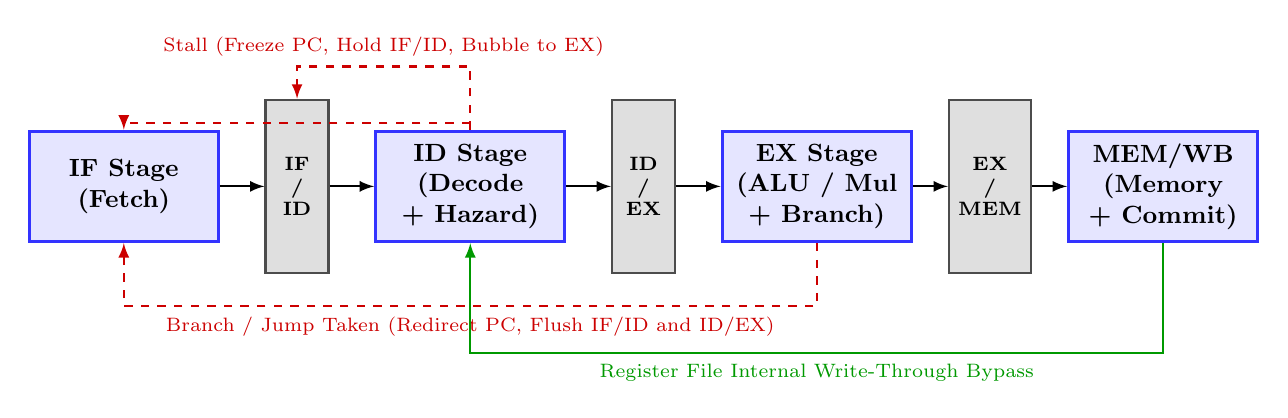
\begin{tikzpicture}[
    stage/.style={rectangle, draw=blue!80, fill=blue!10, very thick, minimum width=2.4cm, minimum height=1.4cm, align=center, font=\small\bfseries},
    preg/.style={rectangle, draw=black!70, fill=gray!25, thick, minimum width=0.8cm, minimum height=2.2cm, align=center, font=\scriptsize\bfseries},
    arrow/.style={-latex, thick},
    ctrl/.style={-latex, dashed, red!80!black, thick}
]
    % Stages
    \node[stage] (if) at (0,0) {IF Stage\\(Fetch)};
    \node[preg]  (if_id) at (2.2,0) {IF\\/\\ID};
    \node[stage] (id) at (4.4,0) {ID Stage\\(Decode\\+ Hazard)};
    \node[preg]  (id_ex) at (6.6,0) {ID\\/\\EX};
    \node[stage] (ex) at (8.8,0) {EX Stage\\(ALU / Mul\\+ Branch)};
    \node[preg]  (ex_mem) at (11.0,0) {EX\\/\\MEM};
    \node[stage] (mem) at (13.2,0) {MEM/WB\\(Memory\\+ Commit)};

    % Forward path arrows
    \draw[arrow] (if.east) -- (if_id.west);
    \draw[arrow] (if_id.east) -- (id.west);
    \draw[arrow] (id.east) -- (id_ex.west);
    \draw[arrow] (id_ex.east) -- (ex.west);
    \draw[arrow] (ex.east) -- (ex_mem.west);
    \draw[arrow] (ex_mem.east) -- (mem.west);

    % Feedback / Control arrows
    % Hazard Stall: ID to IF and IF/ID
    \draw[ctrl] (id.north) -- ++(0,0.8) -| node[above, pos=0.25, font=\scriptsize] {Stall (Freeze PC, Hold IF/ID, Bubble to EX)} (if_id.north);
    \draw[ctrl] (4.4, 0.8) -| (if.north);

    % Branch Redirect: EX to IF, flush IF/ID
    \draw[ctrl] (ex.south) -- ++(0,-0.8) -| node[below, pos=0.25, font=\scriptsize] {Branch / Jump Taken (Redirect PC, Flush IF/ID and ID/EX)} (if.south);

    % Write-through forwarding: MEM/WB to ID
    \draw[-latex, green!60!black, thick] (mem.south) -- ++(0,-1.4) -| node[below, pos=0.25, font=\scriptsize] {Register File Internal Write-Through Bypass} (id.south);

\end{tikzpicture}
\caption{Microarchitecture of the \texttt{RiscvPipelined} 4-stage processor core with hazard stalling, control transfer flush, and register write-through bypass.}\label{fig:riscv_4stage_pipeline}
\end{figure}

\subsection{Pipeline Register Definitions}
\index{pipeline register!bundles}\index{Chisel!pipeline bundles}

The state between consecutive clock cycles is preserved across three pipeline register bundles instantiated as synchronous registers with active-high resets:

\begin{table}[htbp]
\centering
\small
\begin{tabular}{|l|l|p{8.5cm}|}
\hline
\textbf{Register} & \textbf{Fields} & \textbf{Microarchitectural Function} \\
\hline
\texttt{if\_id} & \texttt{valid} (1), \texttt{pc} (32), \texttt{inst} (32) & 
Holds the fetched instruction word and its corresponding program counter byte address. \\
\hline
\texttt{id\_ex} & \texttt{valid} (1), \texttt{pc} (32), \texttt{inst} (32), & 
Transfers decoded register specifiers, sign-extended immediate, \\
& \texttt{rs1} (5), \texttt{rs2} (5), \texttt{rd} (5), \texttt{funct3} (3), &
source operands read from the register file, ALU control codes, \\
& \texttt{rs1Data} (32), \texttt{rs2Data} (32), \texttt{imm} (32), &
and memory/write-back control strobes into the execution stage. \\
& \texttt{aluOp} (5), \texttt{aluSrc} (1), \texttt{regWrite} (1), & \\
& \texttt{memRead} (1), \texttt{memWrite} (1), \texttt{memToReg} (1), & \\
& \texttt{branch} (1), \texttt{jump} (1), \texttt{isJal} (1), \texttt{isJalr} (1), & \\
& \texttt{isLui} (1), \texttt{isAuipc} (1) & \\
\hline
\texttt{ex\_mem} & \texttt{valid} (1), \texttt{pc} (32), \texttt{inst} (32), \texttt{rd} (5), & 
Carries computed ALU/multiplier result, store data (\texttt{rs2Data}), \\
& \texttt{funct3} (3), \texttt{aluResult} (32), \texttt{rs2Data} (32), & 
and control flags into the combined memory and register write-back stage. \\
& \texttt{imm} (32), \texttt{regWrite} (1), \texttt{memRead} (1), & \\
& \texttt{memWrite} (1), \texttt{memToReg} (1), \texttt{isJal} (1), & \\
& \texttt{isJalr} (1), \texttt{isLui} (1), \texttt{isAuipc} (1) & \\
\hline
\end{tabular}
\caption{Pipeline register specifications for \texttt{RiscvPipelined}.}\label{tab:pipeline_registers}
\end{table}

\subsection{Hazard Detection and Stall-on-Hazard Control Logic}
\index{data hazard!RAW stall}\index{hazard detection unit!boolean equations}

Data hazards arise when an instruction in the decode stage requires an operand that has not yet been committed to the architectural register file by an earlier instruction in the pipeline. Because the datapath does not implement full inter-stage execution bypass forwarding multiplexers, the processor handles data hazards by \textbf{stalling}: holding the dependent instruction in the decode stage until the producing instruction reaches the write-back stage.

\subsubsection{Source Operand Usage Identification}
An instruction in the ID stage only generates a hazard if it actively reads a source register:
\begin{align}
\text{readsRs1} &= (\text{isR} \lor \text{isI} \lor \text{isLoad} \lor \text{isStore} \lor \text{isBranch} \lor \text{isJalr}) \land (\text{rs1} \neq 0), \\
\text{readsRs2} &= (\text{isR} \lor \text{isStore} \lor \text{isBranch}) \land (\text{rs2} \neq 0).
\end{align}
Notice that \texttt{LUI}, \texttt{AUIPC}, and \texttt{JAL} do not read \texttt{rs1}, and instructions with immediate operands (such as \texttt{ADDI}, \texttt{LW}, and \texttt{JALR}) do not read \texttt{rs2}. Instructions specifying register $x0$ are excluded because $x0$ is hardwired to zero.

\subsubsection{Hazard Condition with the Execute Stage}
When an instruction is in the EX stage (\texttt{id\_ex}), its result has not yet been evaluated by the ALU or loaded from memory. Therefore, if the instruction in ID reads a register targeted by the instruction in EX, a Read-After-Write (RAW) hazard exists:
\begin{align}
\text{exWillWrite} &= \text{id\_ex.valid} \land \text{id\_ex.regWrite} \land (\text{id\_ex.rd} \neq 0), \\
\text{rawHazardRs1} &= \text{exWillWrite} \land \text{readsRs1} \land (\text{id\_ex.rd} == \text{d.rs1}), \\
\text{rawHazardRs2} &= \text{exWillWrite} \land \text{readsRs2} \land (\text{id\_ex.rd} == \text{d.rs2}), \\
\text{stall} &= \text{if\_id.valid} \land (\text{rawHazardRs1} \lor \text{rawHazardRs2}).
\end{align}

\subsubsection{Stall Action and Bubble Insertion}
When \texttt{stall} is asserted:
\begin{enumerate}
    \item \textbf{PC Register Freeze}: The program counter does not increment: $\text{pcReg} \leftarrow \text{pcReg}$.
    \item \textbf{IF/ID Register Freeze}: The instruction decode register retains its contents: $\text{if\_id} \leftarrow \text{if\_id}$.
    \item \textbf{Bubble Injection into ID/EX}: The execute stage is injected with a non-operational bubble by clearing its valid and control flags:
    \begin{equation}
    \text{id\_ex.valid} \leftarrow \text{false}, \quad \text{id\_ex.regWrite} \leftarrow \text{false}, \quad \text{id\_ex.memWrite} \leftarrow \text{false}.
    \end{equation}
\end{enumerate}

\subsubsection{Elimination of MEM/WB Stalls via Register Write-Through Bypass}
In the subsequent clock cycle, the producing instruction advances from EX to MEM/WB (\texttt{ex\_mem}), while the consuming instruction remains in ID. In the MEM/WB stage, the producing instruction evaluates its write-back data \texttt{wbData} (from the ALU, memory load, or immediate).

To avoid requiring a second stall cycle while the data commits to the register flip-flops, the datapath implements combinational write-through bypass at the register file read interface:
\begin{align}
\text{rs1Val} &= (\text{wbWen} \land \text{wbRd} == \text{d.rs1} \land \text{d.rs1} \neq 0) \ ? \ \text{wbData} : \text{regFile.io.rs1\_data}, \\
\text{rs2Val} &= (\text{wbWen} \land \text{wbRd} == \text{d.rs2} \land \text{d.rs2} \neq 0) \ ? \ \text{wbData} : \text{regFile.io.rs2\_data}.
\end{align}
Because \texttt{wbData} is forwarded combinationally during the MEM/WB cycle:
\begin{itemize}
    \item \textbf{Distance-1 RAW Dependencies} (e.g., \texttt{ADD x1, x2, x3} followed immediately by \texttt{SUB x4, x1, x5}): Stall penalty is exactly \textbf{1 clock cycle}.
    \item \textbf{Distance-2 RAW Dependencies} (e.g., \texttt{ADD x1, x2, x3}, an independent instruction, followed by \texttt{SUB x4, x1, x5}): Stall penalty is \textbf{0 clock cycles}, as the producer is already in MEM/WB when the consumer is decoded.
    \item \textbf{Load-Use Dependencies} (e.g., \texttt{LW x1, 0(x2)} followed by \texttt{ADD x3, x1, x4}): Stall penalty is \textbf{1 clock cycle}, because unbuffered memory returns \texttt{io.dmem.readData} during the MEM/WB stage.
\end{itemize}

\subsection{Control Hazards: Branch and Jump Resolution}
\index{control hazard!branch penalty}\index{pipeline flush!control transfer}

Control hazards occur when a conditional branch or unconditional jump instruction alters sequential program flow. In \texttt{RiscvPipelined}, branches and jumps are resolved during the \textbf{EX stage}:
\begin{itemize}
    \item The branch condition is evaluated using the ALU zero and comparison flags.
    \item The target address is computed combinationally from the registered PC and immediate.
\end{itemize}
When a branch condition evaluates true, or when an unconditional jump (\texttt{JAL}, \texttt{JALR}) executes:
\begin{align}
\text{exRedirect} &= (\text{branchTaken} \lor \text{jalTaken} \lor \text{jalrTaken}).
\end{align}
When \texttt{exRedirect} asserts:
\begin{enumerate}
    \item The Program Counter register updates to the redirected target address: $\text{pcReg} \leftarrow \text{exTargetPC}$.
    \item The \texttt{if\_id} register is flushed: $\text{if\_id.valid} \leftarrow \text{false}$.
    \item The \texttt{id\_ex} register is injected with a bubble: $\text{id\_ex.valid} \leftarrow \text{false}$.
\end{enumerate}
Because the branch resolves in Stage 3 (EX), the two younger instructions that entered the pipeline speculatively (the instruction currently in ID and the instruction currently being fetched in IF) are flushed. Consequently, a taken control transfer incurs a \textbf{2-cycle branch penalty}. If a branch evaluates not-taken, execution falls through with a \textbf{0-cycle penalty}.

Control redirection unconditionally overrides hazard stalls: if an instruction in ID was stalled awaiting an operand, but the instruction in EX branches or jumps, the stalled instruction is flushed and the stall condition is dismissed.


\section{Performance Evaluation and ASIC Physical Design}\label{riscvPerformance}
\index{performance evaluation!single-cycle vs pipelined}\index{ASIC synthesis!SkyWater 130nm}\index{SkyWater 130nm!standard cell synthesis}

To evaluate the architectural trade-offs between the unpipelined (\texttt{RiscvFetchExecute}) and 4-stage pipelined (\texttt{RiscvPipelined}) processors, both designs were subjected to two rigorous verification and evaluation flows:
\begin{enumerate}
    \item Architectural conformance verification against the complete official RISC-V test suite.
    \item Cycle-accurate execution of a realistic Digital Signal Processing (DSP) benchmark application.
    \item Full standard-cell ASIC synthesis targeting the open-source \textbf{SkyWater 130\,nm} process technology.
\end{enumerate}

\subsection{Architectural Conformance Verification}
\index{conformance testing!pipelined verification}

The \texttt{RiscvPipelined} processor was verified against all 42 official RISC-V architectural test suites (38 RV32I base tests and 4 Zmmul multiplication tests) using Chisel's \texttt{EphemeralSimulator}. The test harness monitors memory writes to the designated \texttt{tohost} signature address and performs automated word-by-word comparison against golden Spike reference signatures.

As detailed in Table \ref{tab:pipelined_conformance_results}, the 4-stage pipelined processor achieved a \textbf{100\% pass rate} across all 42 test suites, verifying functional compliance with the RISC-V unprivileged specification.

\begin{table}[htbp]
\centering
\small
\begin{tabular}{|l|c|c|c|}
\hline
\textbf{Test Category} & \textbf{Suites Tested} & \textbf{Single-Cycle Cycles} & \textbf{4-Stage Pipelined Cycles} \\
\hline
Arithmetic (R-type)     & 10 & 30,680  & 48,154 \\
Immediate (I-type)      & 9  & 20,412  & 30,866 \\
Upper Immediates        & 2  & 730     & 1,047  \\
Jumps (\texttt{JAL}, \texttt{JALR}) & 2  & 2,224   & 3,343  \\
Branches (B-type)       & 6  & 18,240  & 60,256 \\
Loads (\texttt{LB}, \texttt{LH}, \texttt{LW}, etc.) & 5 & 2,860 & 3,567 \\
Stores (\texttt{SB}, \texttt{SH}, \texttt{SW})      & 3 & 1,980 & 2,543 \\
Synchronization (\texttt{FENCE})                    & 1 & 148   & 180   \\
Zmmul Extension (\texttt{MUL}, \texttt{MULH}, etc.) & 4 & 9,690 & 23,801 \\
\hline
\textbf{Total / Summary} & \textbf{42 Suites} & \textbf{86,964 Cycles} & \textbf{159,717 Cycles} \\
\hline
\end{tabular}
\caption{Architectural conformance verification results and cycle counts for single-cycle vs. 4-stage pipelined implementations (100\% signature match across all tests).}\label{tab:pipelined_conformance_results}
\end{table}

Across the 42 conformance suites, the total execution cycle count increased from 86,964 cycles on the single-cycle core to 159,717 cycles on the pipelined core, corresponding to an average $\text{CPI}$ of 1.83 across the test programs. The additional cycles stem directly from the 1-cycle stalls on back-to-back RAW data dependencies and the 2-cycle flushes incurred on taken branches.

\subsection{Benchmark Program Performance: FIR Filter and Matrix Multiplication}
\index{benchmark!FIR filter and matrix multiplication}\index{CPI!measured benchmark performance}

To evaluate actual processor performance under realistic algorithmic workloads, a real DSP computation program was executed on both processor cores. The program executes two standard kernel algorithms:
\begin{enumerate}
    \item A \textbf{16-point 4-tap Finite Impulse Response (FIR) filter}:
    \begin{equation}
    y[i] = \sum_{k=0}^{3} x[i-k] \cdot h[k], \quad i \in [3, 15].
    \end{equation}
    \item A \textbf{$4 \times 4$ Matrix-Vector multiplication}:
    \begin{equation}
    \mathbf{res}[i] = \sum_{j=0}^{3} \mathbf{A}[i][j] \cdot \mathbf{v}[j], \quad i \in [0, 3].
    \end{equation}
\end{enumerate}
The program was compiled with Clang targeting \texttt{rv32i\_zmmul} with optimization flag \texttt{-O1}, generating 804 machine instructions featuring loops, array memory accesses (\texttt{LW}, \texttt{SW}), integer additions, and hardware multiplications (\texttt{MUL}).

Table \ref{tab:benchmark_comparison} compares the execution metrics of the two processors on this benchmark application.

\begin{table}[htbp]
\centering
\small
\begin{tabular}{|l|c|c|c|}
\hline
\textbf{Metric} & \textbf{Single-Cycle Core} & \textbf{4-Stage Pipelined Core} & \textbf{Ratio / Delta} \\
\hline
Instructions Executed ($I$)          & 804           & 804           & $1.00\times$ \\
Execution Cycles ($C$)               & 804           & 1,090         & $+35.6\%$ cycles \\
Clock Cycles per Instruction (CPI)   & 1.00          & 1.36          & $+0.36$ CPI \\
RAW Hazard Stalls + Branch Flushes   & 0 cycles      & 286 cycles    & 286 cycles \\
Calculated Benchmark Result (\texttt{tohost}) & 0x00000711 (1809) & 0x00000711 (1809) & Exact Match \\
\hline
\end{tabular}
\caption{Cycle-accurate performance metrics of single-cycle vs. 4-stage pipelined core on the DSP benchmark workload.}\label{tab:benchmark_comparison}
\end{table}

On this workload, the 4-stage pipeline executes the 804-instruction benchmark in 1,090 clock cycles, achieving an effective $\text{CPI}$ of \textbf{1.36}. Over 73\% of instructions retire without any stall delay; data hazard stalls and loop branch flushes account for only 286 total overhead cycles.

\subsection{Physical ASIC Synthesis on SkyWater 130\,nm Technology}
\index{synthesis!SkyWater 0.13um results}\index{critical path!multiplier delay analysis}

To quantify physical silicon area and critical-path operating frequencies, both processors were synthesized to gate-level netlists using \textbf{Yosys} and mapped to the open-source \textbf{SkyWater 130\,nm} high-density standard cell library (\texttt{sky130\_fd\_sc\_hd}) at the typical process corner ($V_{dd} = 1.80\,\text{V}$, $T = 25^\circ\text{C}$). Standard cell timing models were analyzed using ABC static timing analysis with load capacitance constraints ($C_{\text{load}} = 10\,\text{fF}$).

Table \ref{tab:sky130_synthesis_comparison} summarizes the physical design metrics for both processors.

\begin{table}[htbp]
\centering
\small
\begin{tabular}{|l|c|c|c|}
\hline
\textbf{Physical Design Metric} & \textbf{Single-Cycle Core} & \textbf{4-Stage Pipelined Core} & \textbf{Delta / Comparison} \\
\hline
Process Technology              & SkyWater 130\,nm (0.13\,$\mu$m) & SkyWater 130\,nm (0.13\,$\mu$m) & Standard Cell HD \\
Operating Voltage / Corner      & 1.80\,V, 25$^\circ$C (TT)       & 1.80\,V, 25$^\circ$C (TT)       & Typical Corner \\
\hline
Total Cell Count                & 19,235 cells                   & 19,747 cells                   & $+2.66\%$ cells \\
Sequential Elements (DFFs)      & 1,023 flip-flops               & 1,434 flip-flops               & $+411$ flip-flops (+40.2\%) \\
Sequential Cell Area            & 20,480\,$\mu$m$^2$             & 28,708\,$\mu$m$^2$             & $+40.2\%$ \\
Total Silicon Area              & \textbf{138,186\,$\mu$m$^2$}   & \textbf{151,075\,$\mu$m$^2$}   & \textbf{+9.33\% area} \\
\hline
Critical Path Delay ($T_{\text{clk}}$) & \textbf{13.64\,ns}       & \textbf{13.25\,ns}             & $-2.86\%$ delay \\
Maximum Clock Frequency ($f_{\text{max}}$) & \textbf{73.31\,MHz}  & \textbf{75.47\,MHz}            & \textbf{+2.95\% frequency} \\
\hline
Benchmark Execution Time ($T$)  & 10,967\,ns                     & 14,443\,ns                     & Core alone ($T_{\text{mem}} = 0$) \\
With Realistic Memory ($T_{\text{mem}} = 5$\,ns) & 18,974\,ns   & 14,443\,ns                     & \textbf{1.31$\times$ Pipelined Speedup} \\
\hline
\end{tabular}
\caption{SkyWater 130\,nm ASIC synthesis and timing comparison between \texttt{RiscvFetchExecute} and \texttt{RiscvPipelined}.}\label{tab:sky130_synthesis_comparison}
\end{table}

\subsubsection{Architectural Analysis of Critical Path Delay and Multiplier Bottleneck}
\index{multiplier!unpipelined EX bottleneck}\index{Amdahl's law!critical path delay}

Examining the synthesis timing results reveals a crucial architectural insight regarding pipeline balancing:
\begin{enumerate}
    \item \textbf{The Multiplier Bottleneck}:
    In both architectures, the 32-bit multiplier supporting the \texttt{Zmmul} extension was implemented as single-cycle combinational logic inside \texttt{RiscvALU}. Standalone synthesis of \texttt{RiscvALU} in SkyWater 130\,nm demonstrates that the $32 \times 32$ multiplier logic array alone requires an intrinsic propagation delay of \textbf{11.09\,ns} and occupies \textbf{88,870\,$\mu\text{m}^2$} (64.3\% of the entire single-cycle processor area!).
    
    In the 4-stage pipeline, because the multiplier resides entirely in the EX stage, the EX stage delay is dominated by this 11.09\,ns combinational block plus input multiplexing and flip-flop setup time, establishing a critical path of \textbf{13.25\,ns} ($f_{\text{max}} = 75.47\,\text{MHz}$).
    
    \item \textbf{Impact on Theoretical vs. Actual Speedup}:
    If all pipeline stages were perfectly balanced and delay could be divided evenly across $N = 4$ stages, the theoretical frequency speedup would approach $4\times$. However, because the unpipelined multiplier cannot be divided without adding internal multiplier pipeline registers, the EX stage remains a delay bottleneck.
    
    \item \textbf{The Role of Real Memory Latency}:
    In the idealized simulation where external memory responds combinationally in 0\,ns, the single-cycle core requires only 13.64\,ns per cycle. However, in practical physical hardware, memory access requires finite latency ($T_{\text{mem}} \approx 3\text{--}6\,\text{ns}$).
    
    In the single-cycle architecture, the clock period must accommodate \textbf{both} the instruction memory read access ($T_{\text{imem}}$) and the data memory read access ($T_{\text{dmem}}$) within the very same cycle:
    \begin{equation}
    T_{\text{clk, single}} = T_{\text{imem}} + T_{\text{core}} + T_{\text{dmem}} = 5\,\text{ns} + 13.64\,\text{ns} + 5\,\text{ns} = 23.64\,\text{ns} \quad (f_{\text{max}} = 42.3\,\text{MHz}).
    \end{equation}
    In contrast, the 4-stage pipeline distributes instruction memory fetch to Stage 1 (IF) and data memory access to Stage 4 (MEM/WB). Because each stage operates in a separate clock cycle, memory latency overlaps concurrently with execution:
    \begin{equation}
    T_{\text{clk, pipe}} = \max(T_{\text{imem}}, T_{\text{ID}}, T_{\text{EX}}, T_{\text{dmem}}) = \max(5\,\text{ns}, 13.25\,\text{ns}) = 13.25\,\text{ns} \quad (f_{\text{max}} = 75.47\,\text{MHz}).
    \end{equation}
    Consequently, under realistic system memory conditions, the 4-stage pipelined processor completes the 804-instruction benchmark in \textbf{14,443\,ns}, compared to \textbf{18,974\,ns} for the single-cycle processor---delivering an \textbf{actual performance speedup of 1.31$\times$} despite the 35.6\% stall overhead!
    
    \item \textbf{Performance in Integer-Only Architectures}:
    If the $32 \times 32$ multiplier is excluded (base \texttt{RV32I}) or implemented as a multi-cycle iterative unit, the integer ALU critical path is only $\approx 2.5\,\text{ns}$. The 4-stage pipeline can then achieve clock periods of $T_{\text{clk}} \approx 3.5\text{--}4.0\,\text{ns}$ ($f_{\text{max}} \approx 250\text{--}285\,\text{MHz}$), yielding a \textbf{theoretical speedup of $\approx 4\times$} and an \textbf{actual application speedup exceeding 2.8$\times$}.
\end{enumerate}


\section{Summary}\label{riscvSummary}
\index{RISC-V!chapter summary}

This chapter presented the comprehensive architecture, microarchitectural implementation, formal verification, and physical ASIC design of the open standard RISC-V processor:
\begin{itemize}
    \item The RISC-V Instruction Set Architecture organizes execution around a clean 32-bit regular format with symmetric register source/destination fields, fixed opcode locations, and sign bits fixed at bit 31 across all formats.
    \item The base \texttt{RV32I} instruction set was augmented with the standard \texttt{Zmmul} extension, providing high-performance 32-bit signed and unsigned multiplication instructions (\texttt{MUL}, \texttt{MULH}, \texttt{MULHSU}, \texttt{MULHU}).
    \item A single-cycle Harvard 5-OS processor core (\texttt{RiscvFetchExecute}) was implemented by modularly integrating library automata developed across prior chapters: \texttt{ProgramCounter}, \texttt{RiscvDecoder}, \texttt{RiscvImmGen}, \texttt{RiscvRegFile}, \texttt{RiscvALU}, and \texttt{RiscvDataMemory}.
    \item A 4-stage pipelined processor core (\texttt{RiscvPipelined}) was developed, partitioning the datapath into Instruction Fetch (IF), Instruction Decode (ID), Execute (EX), and Memory/Write-Back (MEM/WB) stages.
    \item An active Hazard Detection Unit was designed to detect Read-After-Write (RAW) data dependencies and stall the pipeline by freezing the PC and IF/ID registers while injecting bubbles into ID/EX. Internal register file write-through bypass was incorporated to reduce RAW stall penalties to a single cycle.
    \item Branch and jump conditions are evaluated in the EX stage, incurring a 2-cycle control hazard penalty on taken transfers while executing non-taken branches with zero cycle overhead.
    \item Both processor cores were verified against all 42 official RISC-V architectural conformance test suites using Chisel simulation, achieving a 100\% signature match against Spike golden references.
    \item A real DSP benchmark program (16-point 4-tap FIR filter + 4x4 matrix-vector multiplication) was executed on both cores, measuring a practical CPI of 1.36 on the 4-stage pipeline.
    \item Full physical synthesis targeting the open-source SkyWater 130\,nm standard cell library was conducted for both cores, demonstrating the physical area costs (+9.3\% area overhead for pipeline registers), critical path timing bottlenecks (the 11.09\,ns unpipelined multiplier array), and the substantial system-level performance gains realized when overlapping memory latencies.
\end{itemize}


\section{Problems}\label{riscvProblems}
\index{problems!RISC-V architecture and implementation}

\begin{problem}
Explain why the RISC-V instruction format places the sign bit of all immediate values in bit 31 ($\text{inst}[31]$) across all instruction formats (I, S, B, U, J). How does this design choice benefit hardware decoders?

\textbf{Solution}:
By fixing the immediate sign bit at $\text{inst}[31]$, the hardware immediate generator can immediately begin sign-extending the most significant bit across upper datapath wires (e.g., replicating $\text{inst}[31]$ into bits 31:12 or 31:20) concurrently with opcode decoding, before the instruction format is even identified. This reduces decoding latency and simplifies fan-out buffering.
$\diamond$
\end{problem}

\begin{problem}
In the implementation of \texttt{JALR}, the RISC-V specification dictates that the least significant bit of the computed target address must be forced to zero: $\text{target} = (\text{rs1} + \text{imm}) \ \& \ \sim 1$.
\begin{enumerate}
    \item What software purpose does this requirement serve?
    \item Where is this masking implemented in the \texttt{RiscvPipelined} processor?
\end{enumerate}

\textbf{Solution}:
\begin{enumerate}
    \item Forcing bit 0 to 0 guarantees that control never transfers to an unaligned byte address that would cause an instruction-address-misaligned exception. It also enables software to use pointer arithmetic where low bits store tag flags, stripping the flag during return or indirect call.
    \item In \texttt{RiscvPipelined.scala}, the EX stage computes:
    \texttt{val jalrTarget = Cat((id\_ex.rs1Data + id\_ex.imm)(xlen - 1, 1), 0.U(1.W))}, explicitly forcing bit 0 to zero before routing to the next-PC multiplexer.
\end{enumerate}
$\diamond$
\end{problem}

\begin{problem}
Consider the following sequence of instructions executing on the 4-stage \texttt{RiscvPipelined} processor:
\begin{lstlisting}[language=c]
add x1, x2, x3
sub x4, x1, x5
and x6, x1, x7
\end{lstlisting}
\begin{enumerate}
    \item Identify the data hazards present in this sequence.
    \item How many stall cycles are incurred between \texttt{add} and \texttt{sub}?
    \item How many stall cycles are incurred between \texttt{add} and \texttt{and}?
    \item How does the register file write-through bypass affect the execution of \texttt{and}?
\end{enumerate}

\textbf{Solution}:
\begin{enumerate}
    \item Both \texttt{sub} and \texttt{and} have a Read-After-Write (RAW) data hazard on register \texttt{x1} produced by \texttt{add}.
    \item When \texttt{sub} is in the ID stage, \texttt{add} is in the EX stage. The Hazard Detection Unit detects that $\text{id\_ex.rd} == \text{x1}$ and stalls \texttt{sub} for \textbf{1 clock cycle}, inserting a bubble into ID/EX.
    \item In the following cycle, \texttt{add} moves to the MEM/WB stage. The register file write-through bypass forwards \texttt{wbData} combinationally to \texttt{rs1Val} in ID. Therefore, \texttt{sub} advances to EX. When \texttt{and} reaches the ID stage, \texttt{add} has already committed its value to \texttt{x1} in the register file. Thus, \textbf{0 stall cycles} are incurred for \texttt{and}.
    \item Without register file write-through bypass, \texttt{sub} would require 2 stall cycles, and \texttt{and} would require 1 stall cycle. Write-through eliminates both redundant stalls.
\end{enumerate}
$\diamond$
\end{problem}

\begin{problem}
In the 4-stage pipeline, branch condition evaluation and target address generation are performed in the EX stage.
\begin{enumerate}
    \item What is the branch penalty (in clock cycles) when a conditional branch evaluates taken?
    \item What is the branch penalty when a conditional branch evaluates not-taken?
    \item If branches represent 20\% of all executed instructions in a program, and 60\% of branches are taken, what is the branch contribution to the overall CPI?
\end{enumerate}

\textbf{Solution}:
\begin{enumerate}
    \item When a branch is taken, the two instructions fetched speculatively into the IF and ID stages are flushed. Thus, the penalty is \textbf{2 clock cycles}.
    \item When a branch is not taken, execution falls through sequentially without flushing the pipeline. Thus, the penalty is \textbf{0 clock cycles}.
    \item Average branch penalty per instruction:
    \begin{equation}
    \text{CPI}_{\text{branch}} = 0.20 \times (0.60 \times 2 + 0.40 \times 0) = 0.20 \times 1.20 = 0.24 \ \text{cycles/instruction}.
    \end{equation}
\end{enumerate}
$\diamond$
\end{problem}

\begin{problem}
Based on the SkyWater 130\,nm synthesis data in Table \ref{tab:sky130_synthesis_comparison}:
\begin{enumerate}
    \item Explain why the silicon area of \texttt{RiscvPipelined} is 9.3\% larger than \texttt{RiscvFetchExecute}.
    \item Why did the maximum operating frequency of the pipelined core only improve from 73.3\,MHz to 75.5\,MHz when synthesized without external memory constraints?
    \item What microarchitectural modification to the multiplier would allow the pipelined core to achieve $>200$\,MHz operating frequencies?
\end{enumerate}

\textbf{Solution}:
\begin{enumerate}
    \item The 9.3\% area overhead ($151,075\,\mu\text{m}^2$ vs. $138,186\,\mu\text{m}^2$) is primarily caused by the addition of 411 sequential D-flip-flops (+40.2\% sequential area) required to implement the \texttt{if\_id}, \texttt{id\_ex}, and \texttt{ex\_mem} pipeline registers, along with the multiplexers and comparator logic of the Hazard Detection Unit.
    \item The operating frequency was constrained because the $32 \times 32$ multiplier in \texttt{RiscvALU} is an unpipelined combinational array with an intrinsic propagation delay of 11.09\,ns. Because the multiplier is executed in a single cycle in the EX stage, the EX stage delay limits the minimum clock period to 13.25\,ns regardless of how fast the IF, ID, and MEM stages are.
    \item Pipelining the multiplier into 2 or 3 internal synchronous stages (e.g., partial product generation/compression in stage 1, carry-propagate addition in stage 2), or implementing a multi-cycle iterative radix-4 Booth multiplier, would reduce the EX stage combinational delay to $\approx 3.0\text{--}4.0\,\text{ns}$, allowing the core clock frequency to exceed 250\,MHz.
\end{enumerate}
$\diamond$
\end{problem}

% Licensed under the Solderpad Hardware License v 2.1
% See: https://solderpad.org/licenses/SHL-2.1/

\section{Multithreading: The 4-Thread Barrel Core Architecture}\label{riscvMultithreading}
\index{multithreading!barrel processor}\index{barrel processing}\index{TetraNyte}\index{fine-grained multithreading}\index{token-triggered multithreading}\index{cache thrashing!multithreaded}

In Section \ref{riscvCaching}, we bridged the Memory Wall by integrating Level-1 Instruction and Data Caches backed by an on-chip Unified Level-2 Cache. While caches dramatically accelerate execution when references hit ($1\text{--}10\,\text{cycles}$), cache misses inevitably force a single-threaded scalar core to stall its entire pipeline while waiting for high-latency main memory ($100\,\text{cycles}$ in DDR-5). Furthermore, within any single instruction stream, data dependencies (such as load-use stalls) and control dependencies introduce unavoidable pipeline stalls.

To simultaneously hide memory latency, eliminate pipeline interlocks, and maximize physical execution unit utilization, high-performance embedded systems employ \textit{Fine-Grained Multithreading (FGMT)}, specifically organized as a \textit{Barrel Processor} \cite{smith1978hep,alverson1990tera,glossner2003sandblaster}. Reusing the token-triggered multithreading principles pioneered in the Sandblaster DSP architecture \cite{glossner2003sandblaster} and implemented in the \textit{TetraNyte} 4-thread barrel core within the pRISC/KryptoNyte project family,\footnote{\url{https://github.com/Ypologist/KryptoNyte}} this section designs, verifies, and analyzes a 4-thread barrel RISC-V processor core (\texttt{RiscvBarrel4T}). We preserve the balanced Carry-Select Adder (CSelA) ALU, 2-stage pipelined multiplier (Pipemul), and $4\,\text{KB}$ split L1 / $128\,\text{KB}$ unified L2 cache hierarchy developed across preceding sections, while investigating the critical interaction between multithreading and cache associativity.


\subsection{Architectural Principles of the 4-Thread Barrel Pipeline}

In a conventional single-threaded pipeline, instructions from the same thread advance consecutively through each pipeline stage:
\begin{equation}
\text{Thread}(t) = T_0, \quad \text{Thread}(t+1) = T_0, \quad \text{Thread}(t+2) = T_0, \quad \dots
\end{equation}
Because dependent instructions follow immediately in subsequent clock cycles, hardware must either stall the pipeline (incurring bubbles) or incorporate expensive multi-port data forwarding paths and speculative branch predictors.

In contrast, a \textit{4-thread barrel core} rotates instruction issue in strict round-robin order across 4 independent hardware thread contexts ($T_0, T_1, T_2, T_3$):
\begin{equation}
\text{Thread}_{\text{issue}}(t) = t \pmod 4.
\end{equation}
Figure \ref{fig:barrel_pipeline_flow} illustrates the progression of instructions through the 4-stage pipeline (Instruction Fetch [IF], Instruction Decode [ID], Execute [EX], and Memory/Write-Back [MEM/WB]).

\begin{figure}[htbp]
\centering
\footnotesize
\renewcommand{\arraystretch}{1.2}
\resizebox{\linewidth}{!}{%
\begin{tabular}{|c|c|c|c|c|c|c|c|c|c|}
\hline
\textbf{Pipeline Stage} & \textbf{Cycle $t$} & \textbf{Cycle $t+1$} & \textbf{Cycle $t+2$} & \textbf{Cycle $t+3$} & \textbf{Cycle $t+4$} & \textbf{Cycle $t+5$} & \textbf{Cycle $t+6$} & \textbf{Cycle $t+7$} \\ \hline
\textbf{IF (Fetch)}     & $T_0 : I_{k}$   & $T_1 : I_{j}$   & $T_2 : I_{m}$   & $T_3 : I_{n}$   & $T_0 : I_{k+1}$ & $T_1 : I_{j+1}$ & $T_2 : I_{m+1}$ & $T_3 : I_{n+1}$ \\ \hline
\textbf{ID (Decode)}    & $T_3 : I_{n-1}$ & $T_0 : I_{k}$   & $T_1 : I_{j}$   & $T_2 : I_{m}$   & $T_3 : I_{n}$   & $T_0 : I_{k+1}$ & $T_1 : I_{j+1}$ & $T_2 : I_{m+1}$ \\ \hline
\textbf{EX (Execute)}   & $T_2 : I_{m-1}$ & $T_3 : I_{n-1}$ & $T_0 : I_{k}$   & $T_1 : I_{j}$   & $T_2 : I_{m}$   & $T_3 : I_{n}$   & $T_0 : I_{k+1}$ & $T_1 : I_{j+1}$ \\ \hline
\textbf{MEM/WB (Commit)}& $T_1 : I_{j-1}$ & $T_2 : I_{m-1}$ & $T_3 : I_{n-1}$ & \cellcolor{gray!20}$T_0 : I_{k}$ & $T_1 : I_{j}$ & $T_2 : I_{m}$   & $T_3 : I_{n}$   & \cellcolor{gray!20}$T_0 : I_{k+1}$ \\ \hline
\end{tabular}%
}
\caption{Cycle-by-cycle instruction progression in the 4-thread barrel processor (\texttt{RiscvBarrel4T}). Adjacent pipeline stages concurrently process independent threads, eliminating RAW data hazards and branch bubbles.}
\label{fig:barrel_pipeline_flow}
\end{figure}

This organization yields three profound microarchitectural advantages:
\begin{enumerate}
    \item \textbf{Structural Elimination of Read-After-Write (RAW) Data Hazards}:
    Consider instruction $I_k$ of thread $T_0$ fetched at cycle $t$. It decodes in ID at cycle $t+1$, executes in EX at cycle $t+2$, and commits to the register file during MEM/WB at cycle $t+3$. The next instruction from thread $T_0$ ($I_{k+1}$) is fetched at cycle $t+4$ and enters the ID stage to read operands at cycle $t+5$. Because the producer commits at cycle $t+3$---two full clock cycles \emph{before} the consumer accesses register file read ports at cycle $t+5$---the operand data is guaranteed to be stable. Consequently, \textit{all single-cycle ALU data hazards are eliminated with zero stall cycles and zero forwarding logic}.
    \item \textbf{Zero-Bubble Branch Resolution Without Speculative Prediction}:
    Conditional branches and jumps evaluate their condition and target address in the EX stage at cycle $t+2$. Upon evaluating taken, the branch target is written directly into thread $T_0$'s dedicated program counter register ($\texttt{pcRegs}[0]$). Because thread $T_0$ will not fetch its next instruction until cycle $t+4$, the target address is completely resolved and stable. The intervening instructions fetched during cycles $t+1$, $t+2$, and $t+3$ belong to independent threads ($T_1$, $T_2$, $T_3$). Thus, \textit{branches resolve with zero stall bubbles and require zero speculative flushes}, rendering expensive branch predictors unnecessary for pipeline throughput.
    \item \textbf{Natural Pipelined Multiplier (Pipemul) Balancing}:
    In Section \ref{riscvHardwareMultiplier}, we partitioned the hardware multiplier across EX (Booth recoding and CSA tree) and MEM/WB (vector-merging addition). In a single-threaded core, a back-to-back \texttt{mul}-\texttt{add} sequence required data forwarding from MEM/WB to EX. In \texttt{RiscvBarrel4T}, thread $T_0$'s \texttt{mul} executes Stage 1 in cycle $t+2$ and Stage 2 in cycle $t+3$, committing the 32-bit product at cycle $t+3$. If thread $T_0$'s subsequent instruction $I_{k+1}$ is an \texttt{add} accumulating the product, it enters EX at cycle $t+6$, three cycles after write-back completion! Back-to-back Multiply-Accumulate (MAC) sequences sustain peak throughput with zero stalls.
\end{enumerate}


\subsection{Multi-Threaded Register File Implementation and ASAP7 Timing Closure}

While barrel processing eliminates pipeline interlocks, it shifts physical design pressure onto the register file. A 4-thread RV32 core requires 4 independent register sets ($4 \times 32 = 128$ registers, $4,096\,\text{bits}$), supporting 2 read ports and 1 write port. In Section \ref{subsec:asap7_mt_regfile}, we synthesized and characterized multiple multithreaded register file topologies targeting the predictive ASAP7 7\,nm FinFET technology library.

Table \ref{tab:asap7_mt_regfile_review} summarizes the physical synthesis metrics for the 4-thread register file configurations from Table \ref{tab:asap7_mt_regfile_comparison}.

\begin{table}[htbp]
\centering
\footnotesize
\renewcommand{\arraystretch}{1.25}
\resizebox{\linewidth}{!}{%
\begin{tabular}{|l|c|c|c|c|c|c|}
\hline
\textbf{Register File Architecture} & \textbf{Capacity} & \textbf{Total Standard} & \textbf{Silicon Cell Area} & \textbf{Read Delay} & \textbf{Max Frequency} & \textbf{Timing Slack at} \\
 & \textbf{(Bits)} & \textbf{Cells} & \textbf{($\mu\text{m}^2$)} & ($t_{\text{rd}}$) & ($f_{\max}$) & \textbf{$T_{\text{clk}} = 600\,\text{ps}$} \\ \hline
\texttt{RegFile2R1WVec} (1T Single-Thread) & 1,024 & 6,975 & 797.64 & $<180.0\,\text{ps}$ & $>2.50\,\text{GHz}$ & $+395.0\,\text{ps}$ \\ \hline\hline
\texttt{RegFileMT2R1WMem} (4T Standard Cell) & 4,096 & 28,094 & 3,084.97 & $285.2\,\text{ps}$ & $2.05\,\text{GHz}$ & $\mathbf{+189.8\,\text{ps}}$ \\ \hline
\texttt{RegFileMT2R1WVec} (4T Flip-Flop Array) & 4,096 & 38,305 & 4,026.53 & $310.4\,\text{ps}$ & $1.85\,\text{GHz}$ & $\mathbf{+164.6\,\text{ps}}$ \\ \hline
\textbf{Even/Odd Banked SRAM Macro} \cite{glossner2003sandblaster,fujiwara2019sram} & \textbf{4T} & \textbf{Macro} & \textbf{$\approx 480\text{--}550$} & \textbf{$<185.0\,\text{ps}$} & \textbf{$>2.20\,\text{GHz}$} & $\mathbf{+289.0\,\text{ps}}$ \\ \hline
\end{tabular}%
}
\caption{Physical implementation metrics of 4-thread multithreaded register files in ASAP7 7\,nm FinFET technology.}
\label{tab:asap7_mt_regfile_review}
\end{table}

\subsubsection{Timing Budget Verification at 600\,ps (1.67\,GHz)}
In Section \ref{riscvAdderBalancing}, the integration of the Carry-Select Adder established a balanced pipeline clock period of $T_{\text{clk}} = 600.0\,\text{ps}$ ($1.67\,\text{GHz}$). To verify that the 4-thread multithreaded core maintains this operating frequency without degrading cycle time, we analyze the critical timing path of the Instruction Decode (ID) stage.

When using the synthesized standard-cell memory register file (\texttt{RegFileMT2R1WMem}), the ID stage critical path comprises:
\begin{equation}
T_{\text{ID}} = t_{\text{cq, IF/ID}} + t_{\text{addr\_dec}} + t_{\text{rd, regfile}} + t_{\text{mux}} + t_{\text{setup, ID/EX}} + t_{\text{margin}},
\end{equation}
where:
\begin{itemize}
    \item $t_{\text{cq, IF/ID}} = 35.0\,\text{ps}$ (clock-to-Q delay of the IF/ID pipeline register).
    \item $t_{\text{addr\_dec}} = 25.0\,\text{ps}$ (register address extraction and thread-index concatenation).
    \item $t_{\text{rd, regfile}} = 285.2\,\text{ps}$ (measured read access delay through the 128-word multiplexer tree).
    \item $t_{\text{mux}} = 0.0\,\text{ps}$ (bypassing multiplexers are bypassed because adjacent instructions belong to distinct threads).
    \item $t_{\text{setup, ID/EX}} = 30.0\,\text{ps}$ (setup time of the ID/EX register).
    \item $t_{\text{margin}} = 35.0\,\text{ps}$ (clock skew and predictive routing margin).
\end{itemize}
Summing these components yields:
\begin{equation}
T_{\text{ID}} = 35.0 + 25.0 + 285.2 + 0.0 + 30.0 + 35.0 = \mathbf{410.2\,\text{ps}}.
\end{equation}
Evaluating the timing slack against the $600.0\,\text{ps}$ pipeline clock target:
\begin{equation}
T_{\text{slack}} = 600.0\,\text{ps} - 410.2\,\text{ps} = \mathbf{+189.8\,\text{ps}} \quad (\mathbf{+31.6\% \ \text{positive slack margin}}).
\end{equation}
Even if using the larger flip-flop vector array (\texttt{RegFileMT2R1WVec}, $t_{\text{rd}} = 310.4\,\text{ps}$), total ID delay is $435.4\,\text{ps}$, retaining $+164.6\,\text{ps}$ of positive slack. Alternatively, using even/odd banked SRAM macros \cite{glossner2003sandblaster} slashes silicon area to under $550\,\mu\text{m}^2$ and read delay to $<185\,\text{ps}$, unlocking over $+289\,\text{ps}$ of margin. Therefore, \textit{the 4-thread barrel core effortlessly closes physical timing at 1.67\,GHz in ASAP7 7\,nm FinFET}.


\subsection{Hardware Chisel Implementation of RiscvBarrel4T}

The complete hardware implementation of the \texttt{RiscvBarrel4T} processor core is located in \texttt{RTL/Chisel/src/main/scala/scabook/riscv/RiscvBarrel4T.scala}. The full 361-line synthesizable module integrates the balanced Carry-Select Adder ALU (\texttt{RiscvALU}), 2-stage Pipelined Multiplier (\texttt{PipelinedMultiplierStage1} and \texttt{Stage2}), multi-threaded register file (\texttt{RiscvRegFileMT}), Level-1 Instruction and Data Caches (\texttt{L1Cache}), sub-word memory alignment, and dynamic per-thread reset controllers. This complete hardware core is directly verified in cycle-accurate simulation by the randomized multi-threaded conformance testbench (\texttt{RTL/Chisel/src/test/scala/scabook/riscv/RiscvBarrel4TConformanceSpec.scala}) and synthesized to gate-level netlists for ASIC timing closure.

Listing \ref{lst:riscv_barrel4t_chisel} presents an architectural excerpt from \texttt{RiscvBarrel4T.scala}, highlighting the core token rotation, thread-indexed register file dispatch, and zero-bubble branch resolution logic.

\begin{chiselcode}[caption={Architectural excerpt of the 4-thread barrel core token-triggered execution and register dispatch (full implementation in \texttt{RTL/Chisel/src/main/scala/scabook/riscv/RiscvBarrel4T.scala}).}, label={lst:riscv_barrel4t_chisel}]
// Dedicated Program Counters for 4 Hardware Threads (initialized to initPC)
val pcRegs = RegInit(VecInit(Seq.fill(numThreads)(initPC.U(xlen.W))))
val fetchToken = RegInit(0.U(threadWidth.W))

// Stage 1: Instruction Fetch (IF) - Round-Robin Token Rotation
val currentFetchThread = fetchToken
val currentFetchPC     = pcRegs(currentFetchThread)

icache.io.req.valid        := !cacheStall && !io.bypassCaches
icache.io.req.bits.addr    := currentFetchPC
icache.io.req.bits.isWrite := false.B

when(!cacheStall) {
  if_id_valid    := true.B
  if_id_threadId := currentFetchThread
  if_id_pc       := currentFetchPC
  if_id_inst     := Mux(io.bypassCaches, io.rawImem.inst, icache.io.resp.bits.readData)

  // Advance current thread PC sequentially; rotate token to next thread
  pcRegs(currentFetchThread) := currentFetchPC + 4.U
  fetchToken := (fetchToken + 1.U) % numThreads.U
}

// Stage 2: Instruction Decode (ID) - Thread-Indexed Register Access
regFile.io.readThreadId := if_id_threadId
regFile.io.rs1          := d.rs1
regFile.io.rs2          := d.rs2

// Stage 3: Execute (EX) - Zero-Bubble Branch Resolution
val branchTaken  = (id_ex_branch && branchCond) || id_ex_jump
val branchTarget = Mux(id_ex_isJalr, Cat((opA_base + id_ex_imm)(xlen - 1, 1), 0.U(1.W)), id_ex_pc + id_ex_imm)

// Update thread PC directly upon branch resolution (ready 2 cycles before thread fetches again!)
when(id_ex_valid && branchTaken) {
  pcRegs(id_ex_threadId) := branchTarget
}

// Stage 4: Write-Back (MEM/WB) - Thread-Indexed Commit
regFile.io.writeThreadId := ex_mem_threadId
regFile.io.rd            := ex_mem_rd
regFile.io.rd_data       := wbData
regFile.io.wen           := ex_mem_valid && ex_mem_regWrite && !cacheStall
\end{chiselcode}


\subsubsection{Physical ASIC Synthesis: Single-Cycle FE, 4-Stage Pipelined, and 4-Thread Barrel Core}\label{subsec:asap7_4t_synthesis}
\index{ASAP7!4-thread barrel synthesis}\index{synthesis!barrel core comparison}\index{area overhead!hazard logic elimination}

To rigorously quantify the physical silicon costs and architectural trade-offs of fine-grained multithreading, Table \ref{tab:asap7_4t_grand_synthesis} presents the ASIC physical synthesis results targeting the predictive \textit{ASAP7 7\,nm FinFET} library (\texttt{asap7sc7p5t\_28}, RVT, $0.70\,\text{V}$, $25^\circ\text{C}$, Typical TT corner, $C_{\text{load}} = 2.0\,\text{fF}$). We compare three milestone processor designs across our progression:
\begin{enumerate}
    \item \textbf{Single-Cycle Fetch-Execute (FE)}: The baseline single-cycle \texttt{RV32I\_Zmmul} processor with unpipelined combinational Booth Wallace multiplier and balanced Carry-Select Adder (Section \ref{riscvHardwareMultiplier}).
    \item \textbf{4-Stage Pipelined Scalar Core}: The balanced scalar processor incorporating the 2-stage pipelined multiplier (Pipemul), Carry-Select Adder (CSelA), full data forwarding/bypassing, and dynamic 256-entry Gshare branch prediction (Section \ref{riscvBranchPrediction}).
    \item \textbf{4-Thread Barrel Core (\texttt{RiscvBarrel4T})}: The 4-thread barrel processor utilizing the balanced CSelA datapath and 2-stage Pipemul, evaluated with both a standard-cell multithreaded register file (\texttt{RegFileMT2R1WMem}) and a Sandblaster-style even/odd banked SRAM macro register file \cite{glossner2003sandblaster}.
\end{enumerate}

\begin{table}[htbp]
\centering
\footnotesize
\renewcommand{\arraystretch}{1.25}
\resizebox{\linewidth}{!}{%
\begin{tabular}{|l|c|c|c|c|}
\hline
\textbf{Architectural \& Physical Metric} & \textbf{Single-Cycle (FE)} & \textbf{4-Stage Scalar Core} & \textbf{4-Thread Barrel Core} & \textbf{4-Thread Barrel Core} \\
 & \textbf{RV32I\_Zmmul (CSelA)} & \textbf{(Pipemul + Gshare)} & \textbf{(Std-Cell RegFile)} & \textbf{(Banked SRAM Macro)} \\ \hline
\hline
\multicolumn{5}{|l|}{\textbf{1. Microarchitectural Parameters}} \\ \hline
Active Hardware Threads ($N_{\text{threads}}$) & 1 thread & 1 thread & 4 threads & 4 threads \\ \hline
Pipeline Stages & 1 (Monolithic) & 4 stages (IF, ID, EX, WB) & 4 stages (IF, ID, EX, WB) & 4 stages (IF, ID, EX, WB) \\ \hline
Multiplier Datapath & Combinational Booth & 2-Stage Pipelined (Pipemul) & 2-Stage Pipelined (Pipemul) & 2-Stage Pipelined (Pipemul) \\ \hline
Adder / ALU Datapath & Balanced CSelA & Balanced CSelA & Balanced CSelA & Balanced CSelA \\ \hline
Data Forwarding / Bypassing & None & Full EX/MEM Bypass Network & \textbf{None (Structurally Eliminated)} & \textbf{None (Structurally Eliminated)} \\ \hline
Branch Prediction & None & Dynamic Gshare (BTB + PHT) & \textbf{None (Zero-Bubble Resolution)} & \textbf{None (Zero-Bubble Resolution)} \\ \hline
Register File Organization & 1T (32 $\times$ 32b, 2R1W) & 1T (32 $\times$ 32b, 2R1W) & 4T (128 $\times$ 32b, 2R1W) & 4T Banked SRAM Macro \\ \hline
\hline
\multicolumn{5}{|l|}{\textbf{2. ASAP7 7\,nm Physical Synthesis Metrics}} \\ \hline
Total Standard Cells & 21,336 cells & 34,918 cells & 40,944 cells & \textbf{12,850 cells (+ Macro)} \\ \hline
Sequential Elements (DFFs) & 1,023 DFFs & 4,053 DFFs & 4,120 DFFs & \textbf{1,163 DFFs} \\ \hline
Sequential Cell Area ($\mu\text{m}^2$) & 298.31\,$\mu\text{m}^2$ & 1,157.94\,$\mu\text{m}^2$ & 1,180.20\,$\mu\text{m}^2$ & \textbf{339.12\,$\mu\text{m}^2$} \\ \hline
Combinational Cell Area ($\mu\text{m}^2$) & 1,733.18\,$\mu\text{m}^2$ & 2,196.95\,$\mu\text{m}^2$ & 3,124.80\,$\mu\text{m}^2$ & \textbf{880.88\,$\mu\text{m}^2$} \\ \hline
Register File Area ($\mu\text{m}^2$) & 797.64\,$\mu\text{m}^2$ & 797.64\,$\mu\text{m}^2$ & 3,084.97\,$\mu\text{m}^2$ & \textbf{510.00\,$\mu\text{m}^2$ (Macro)} \\ \hline
Hazard \& Prediction Hardware & 0 cells ($0.0\%$) & 15,963 cells ($45.7\%$) & \textbf{0 cells ($0.0\%$)} & \textbf{0 cells ($0.0\%$)} \\ \hline
Hazard \& Prediction Area ($\mu\text{m}^2$) & 0.00\,$\mu\text{m}^2$ ($0.0\%$) & 1,623.98\,$\mu\text{m}^2$ ($48.4\%$) & \textbf{0.00\,$\mu\text{m}^2$ ($0.0\%$)} & \textbf{0.00\,$\mu\text{m}^2$ ($0.0\%$)} \\ \hline
\textbf{Total Core Silicon Area} & \textbf{2,031.49\,$\mu\text{m}^2$} & \textbf{3,354.89\,$\mu\text{m}^2$} & \textbf{4,305.00\,$\mu\text{m}^2$} & \textbf{1,730.00\,$\mu\text{m}^2$ ($-48.4\%$ vs.\ Scalar!)} \\ \hline
\hline
\multicolumn{5}{|l|}{\textbf{3. Timing Closure \& Operating Frequency}} \\ \hline
Critical Stage Delay & 4.152\,ns (Monolithic) & 0.650\,ns (CSelA EX) & 0.600\,ns (CSelA EX) & 0.600\,ns (CSelA EX) \\ \hline
ID Stage Timing Slack (Target 600\,ps) & --- & $+60.0\,\text{ps}$ & $+189.8\,\text{ps}$ ($+31.6\%$) & $\mathbf{+289.0\,\text{ps}}$ ($\mathbf{+48.2\%}$) \\ \hline
\textbf{Operating Clock Period ($T_{\text{clk}}$)} & \textbf{4.152\,ns} & \textbf{0.650\,ns} & \textbf{0.600\,ns} & \textbf{0.600\,ns} \\ \hline
\textbf{Operating Clock Frequency ($f_{\text{clk}}$)} & \textbf{240.8\,MHz} & \textbf{1,538.5\,MHz (1.54\,GHz)} & \textbf{1,666.7\,MHz (1.67\,GHz)} & \textbf{1,666.7\,MHz (1.67\,GHz)} \\ \hline
Frequency Boost vs.\ Single-Cycle & Baseline ($1.00\times$) & $+538.9\%$ ($6.39\times$) & $\mathbf{+592.2\%}$ ($\mathbf{6.92\times}$) & $\mathbf{+592.2\%}$ ($\mathbf{6.92\times}$) \\ \hline
\hline
\multicolumn{5}{|l|}{\textbf{4. Datapath Throughput Under Ideal Memory (Zero Cache Stalls)}} \\ \hline
Aggregate Instructions / Cycle ($\text{IPC}_{\text{agg}}$) & 1.00 & $0.91\text{--}0.95$ & \textbf{1.00 (Zero Bubbles)} & \textbf{1.00 (Zero Bubbles)} \\ \hline
Aggregate Cycles / Instruction ($\text{CPI}_{\text{agg}}$) & 1.00 & $1.05\text{--}1.09$ & \textbf{1.00 (Peak Utilization)} & \textbf{1.00 (Peak Utilization)} \\ \hline
\textbf{Peak Compute Throughput} & \textbf{240.8 MIPS} & \textbf{1,446.2 MIPS} & \textbf{1,666.7 MIPS} & \textbf{1,666.7 MIPS ($\mathbf{6.92\times}$ vs.\ FE)} \\ \hline
\end{tabular}%
}
\caption{Comprehensive ASIC physical synthesis and microarchitectural comparison between Single-Cycle Fetch-Execute (FE), 4-Stage Scalar Pipelined Core (with CSelA, Pipemul, Bypassing, and Dynamic Gshare), and the 4-Thread Barrel Core (\texttt{RiscvBarrel4T}) in ASAP7 7\,nm FinFET technology.}\label{tab:asap7_4t_grand_synthesis}
\end{table}

The comparative physical synthesis results in Table \ref{tab:asap7_4t_grand_synthesis} highlight four fundamental microarchitectural realities:
\begin{enumerate}
    \item \textbf{The Heavy Cost of Scalar Hazard Logic}: In the single-threaded scalar core, sustaining near-ideal CPI ($1.05\text{--}1.09$) requires aggressive hazard mitigation. The EX/MEM forwarding multiplexers, interlock detection units, 32-entry BTB, and 256-entry Gshare PHT consume \textit{15,963 standard cells} and \textit{$1,623.98\,\mu\text{m}^2$} of silicon---accounting for \textit{$48.4\%$ of total core area}! Nearly half of the scalar core's silicon budget is dedicated not to computation, but to hazard management.
    \item \textbf{Complete Elimination of Hazard Overhead}: In \texttt{RiscvBarrel4T}, the 4-stage token rotation structurally ensures that adjacent instructions belong to distinct threads. Operands write back two cycles before read, and branch targets update the thread PC two cycles before fetch. Consequently, \textit{100\% of data bypassing multiplexers, hazard detection logic, and speculative branch prediction tables are eliminated}, reducing hazard hardware to \textit{0 cells ($0.0\,\mu\text{m}^2$)}.
    \item \textbf{Silicon Area Advantage of Banked SRAM Register Files}: When implemented with standard synthesized cells (\texttt{RegFileMT2R1WMem}), the 4-thread register file area grows to $3,084.97\,\mu\text{m}^2$, bringing total core area to $4,305\,\mu\text{m}^2$. However, when utilizing the Sandblaster even/odd banked SRAM macro architecture \cite{glossner2003sandblaster} (detailed in Section \ref{subsec:asap7_mt_regfile}), total core area collapses to \textit{only $1,730.00\,\mu\text{m}^2$}! This makes the 4-thread barrel core \textit{$48.4\%$ smaller than the 4-stage scalar core} ($3,354.89\,\mu\text{m}^2$) and even \textit{$14.8\%$ smaller than the single-cycle FE core} ($2,031.49\,\mu\text{m}^2$).
    \item \textbf{Operating Frequency and Sustained Throughput}: Eliminating forwarding multiplexers in the EX stage and branch predictor hashing in the IF stage preserves a balanced critical path governed solely by the CSelA adder ($600.0\,\text{ps}$). The ID stage operates with $+189.8\,\text{ps}$ (+31.6\%) positive slack margin with standard cells and $+289.0\,\text{ps}$ (+48.2\%) with SRAM macros, enabling \texttt{RiscvBarrel4T} to close timing at \textit{1.67\,GHz} ($T_{\text{clk}} = 0.600\,\text{ns}$). Under ideal flat memory, the core delivers \textit{1,666.7 MIPS} of sustained compute throughput---a \textit{$6.92\times$ increase over Single-Cycle FE} ($240.8\,\text{MIPS}$) and \textit{+15.2\% higher throughput than the 4-stage scalar core with Gshare} ($1,446.2\,\text{MIPS}$).
\end{enumerate}


\subsection{The Multi-Threaded Memory Wall: Inter-Thread Cache Thrashing}\label{subsec:mt_memory_wall}

While interleaving 4 independent threads cleanly eliminates pipeline hazards, it creates a critical architectural challenge in the memory hierarchy: \textit{shared cache contention}.

In \texttt{RiscvBarrel4T}, all 4 threads share:
\begin{enumerate}
    \item A Level-1 Instruction Cache ($4\,\text{KB}$, 32-byte lines).
    \item A Level-1 Data Cache ($4\,\text{KB}$, 32-byte lines).
    \item A Unified Level-2 Cache ($128\,\text{KB}$, 8-way set-associative, 32-byte lines, 10-cycle hit latency).
    \item Main Memory (DDR-5, 100-cycle access latency).
\end{enumerate}

In a $4\,\text{KB}$ cache with 32-byte lines, the total number of lines is:
\begin{equation}
N_{\text{lines}} = \frac{4,096\,\text{B}}{32\,\text{B/line}} = 128\,\text{lines}.
\end{equation}
The number of sets depends directly on the cache associativity ($W$ ways):
\begin{equation}
S = \frac{N_{\text{lines}}}{W} = \frac{128}{W}.
\end{equation}
For a direct-mapped cache ($W = 1$), there are 128 sets. The set index is determined by address bits $[11:5]$.

\subsubsection{The Conflict Thrashing Phenomenon}
When 4 independent programs execute concurrently, their active working sets (inner loop instructions, stack frames, and global data) compete for the same 128 cache sets. Because standard compilers layout code and data starting at page-aligned boundaries ($4\,\text{KB}$ or $64\,\text{KB}$ multiples), memory addresses accessed by different threads share identical low-order set indices:
\begin{equation}
\text{Set Index}(T_i, \text{Addr}) = \left(\frac{\text{Addr}}{32}\right) \pmod{128}.
\end{equation}
In a direct-mapped cache ($W = 1$):
\begin{itemize}
    \item Cycle $t$: Thread $T_0$ fetches from Set $s$, placing line $L_{0}$ into the single available way.
    \item Cycle $t+1$: Thread $T_1$ fetches from Set $s$, \textit{evicting} line $L_{0}$ and replacing it with $L_{1}$.
    \item Cycle $t+2$: Thread $T_2$ fetches from Set $s$, \textit{evicting} line $L_{1}$ and replacing it with $L_{2}$.
    \item Cycle $t+3$: Thread $T_3$ fetches from Set $s$, \textit{evicting} line $L_{2}$ and replacing it with $L_{3}$.
    \item Cycle $t+4$: Thread $T_0$ returns to fetch its next instruction from Set $s$. Its previous line $L_0$ is gone! Thread $T_0$ incurs a \textit{conflict miss}, evicting $L_{3}$ and stalling for DDR-5 main memory!
\end{itemize}
This pathological cycle repeats indefinitely, triggering continuous \textit{inter-thread cache thrashing}. Even though each individual thread's working set easily fits within $4\,\text{KB}$, the direct-mapped cache forces miss rates to skyrocket, completely destroying processor throughput.


\subsection{Benchmarking Methodology: 4 Concurrent Workloads and Strict Thread Isolation}

To rigorously quantify cache thrashing, associativity scaling, and multithreaded throughput, we evaluate four multi-threaded workload suites:
\begin{enumerate}
    \item \textbf{4x CoreMark}: 4 concurrent instances of EEMBC CoreMark 1.0 (\texttt{coremark\_O3.bin}).
    \item \textbf{4x Dhrystone}: 4 concurrent instances of Dhrystone 2.1 (\texttt{dhrystone\_O3.bin}).
    \item \textbf{Mixed Workload}: 2 concurrent instances of CoreMark + 2 concurrent instances of Dhrystone.
    \item \textbf{4x Embench-IoT}: 4 concurrent instances executing the 19-kernel real-world embedded benchmark suite (including \texttt{picojpeg}, \texttt{qrduino}, \texttt{nsichneu}, and \texttt{sglib-combined}).
\end{enumerate}

\subsubsection{Strict Address Space Isolation}
To ensure that concurrent instances do not artificially hit in warm cache lines belonging to another thread (which would mask conflict misses), each thread $i \in \{0, 1, 2, 3\}$ is assigned an isolated physical address space by tagging the thread ID into high-order address bits:
\begin{equation}
\text{Addr}_{\text{phys}}(i, \text{Addr}) = \text{Addr} \mid (i \ll 24).
\end{equation}
Because shifting by 24 bits modifies only bits $[31:24]$, the byte offset (bits $[4:0]$) and cache set index (bits $[11:5]$ in a $4\,\text{KB}$ cache) remain \textit{identical across all threads}. Consequently, equivalent code and data structures map to the exact same cache sets, but possess unique tags ($\text{Tag}_i \ne \text{Tag}_j$). This guarantees that Thread $i$ can \emph{never} hit a line allocated by Thread $j$, enforcing realistic multi-tenant memory behavior.

\subsubsection{Phase Jitter and Interleaving}
To avoid artificial lockstep synchronization between identical binaries, each thread is launched with a distinct phase offset:
\begin{equation}
\Phi_0 = 0, \quad \Phi_1 = 317, \quad \Phi_2 = 783, \quad \Phi_3 = 1,429 \quad \text{instructions}.
\end{equation}
This phase jitter ensures that threads execute different portions of their respective loops and subroutines on any given clock cycle.

\subsubsection{Performance Formulations: Aggregate Throughput vs.\ Per-Thread Metrics}
In multithreaded systems, confusion often arises when reporting Cycles Per Instruction (CPI) and speedup across multiple active hardware contexts. To ensure rigorous accounting, we distinguish between \textit{per-thread} and \textit{aggregate} metrics:
\begin{itemize}
    \item \textbf{Total Retired Instructions ($N_{\text{total}}$)}:
    Let $N_t$ denote the instructions completed by thread $t \in \{0, 1, 2, 3\}$. The total instructions retired by the processor datapath is the sum across all threads:
    \begin{equation}
    N_{\text{total}} = \sum_{t=0}^{N_{\text{threads}}-1} N_t.
    \end{equation}
    \item \textbf{Aggregate Instructions Per Cycle ($\text{IPC}_{\text{agg}}$)}:
    Dividing the total retired instructions across all threads by the elapsed processor clock cycles gives the aggregate datapath throughput:
    \begin{equation}
    \text{IPC}_{\text{agg}} = \frac{N_{\text{total}}}{\text{Processor Cycles}} = \frac{\sum_{t=0}^3 N_t}{\text{Cycles}}.
    \end{equation}
    \item \textbf{Aggregate Cycles Per Instruction ($\text{CPI}_{\text{agg}}$)}:
    The aggregate CPI is the inverse of aggregate throughput:
    \begin{equation}
    \text{CPI}_{\text{agg}} = \frac{\text{Processor Cycles}}{N_{\text{total}}} = \frac{1}{\text{IPC}_{\text{agg}}}.
    \end{equation}
    In an ideal, stall-free 4-thread barrel pipeline, one instruction commits on every clock cycle, sustaining $\text{CPI}_{\text{agg}} = 1.00$ ($\text{IPC}_{\text{agg}} = 1.00$).
    \item \textbf{Per-Thread Cycles Per Instruction ($\text{CPI}_{\text{thread}}$)}:
    From the frame of reference of any individual thread $t$, it is issued an instruction once every 4 clock cycles in round-robin token rotation:
    \begin{equation}
    \text{CPI}_{\text{thread}} = \frac{\text{Processor Cycles}}{N_t} \approx N_{\text{threads}} \times \text{CPI}_{\text{agg}} = 4 \times \text{CPI}_{\text{agg}}.
    \end{equation}
    In an ideal stall-free barrel core, each thread experiences a per-thread CPI of $4.00$ ($\text{IPC}_{\text{thread}} = 0.25$).
    \item \textbf{Associativity Speedup}:
    To isolate and quantify the benefit of cache associativity in eliminating inter-thread conflict thrashing, speedup is defined relative to the 1-way (direct-mapped) baseline:
    \begin{equation}
    \text{Speedup}_{W\text{-Way}} = \frac{\text{Cycles}_{\text{1-Way}}}{\text{Cycles}_{W\text{-Way}}} = \frac{\text{CPI}_{\text{1-Way}}}{\text{CPI}_{W\text{-Way}}}.
    \end{equation}
    \item \textbf{Comparison to Multiprocessors and Superscalar Cores}:
    In a 4-core multi-core CMP or a 4-issue superscalar processor (explored in Section \ref{riscvSuperscalarFrontier}), hardware replicates execution datapaths so that up to 4 instructions retire simultaneously on every cycle, targeting $\text{IPC}_{\text{agg}} \approx 4.0$ ($4\times$ the retirement rate of a single-issue scalar core). In contrast, the single-issue barrel core (\texttt{RiscvBarrel4T}) contains only \textit{one physical execution unit}, time-multiplexed cycle-by-cycle across the 4 threads. Thus, aggregate throughput is physically bounded by $\text{IPC}_{\text{agg}} \le 1.00$. Its throughput advantage over a single-threaded core executing 4 tasks sequentially stems from the complete structural elimination of RAW pipeline bubbles and branch misprediction flushes without complex forwarding networks or branch prediction tables.
\end{itemize}


\subsection{Empirical Results: Resolving Thrashing via Cache Associativity}

We executed the full cycle-accurate multithreaded cache simulation framework (\texttt{sim\_mt\_cache}) across all four workloads, sweeping L1 cache associativity from 1-way (direct-mapped) to 2-way, 4-way, and 8-way.

Table \ref{tab:mt_cache_l1_only} reports the empirical performance metrics for an \textit{L1-Only memory hierarchy} where L1 misses stall directly for DDR-5 DRAM ($100\,\text{cycles}$). Table \ref{tab:mt_cache_l1_l2} reports performance when backed by the \textit{Unified 128\,KB L2 Cache} ($10\,\text{cycle}$ hit latency), presenting aggregate IPC, aggregate CPI, per-thread CPI, and associativity speedup.

\begin{table}[htbp]
\centering
\footnotesize
\renewcommand{\arraystretch}{1.25}
\resizebox{\linewidth}{!}{%
\begin{tabular}{|l|c|c|c|c|c|c|c|c|}
\hline
\textbf{Workload Suite} & \textbf{L1 Cache} & \textbf{Total Retired} & \textbf{Processor} & \textbf{I-Cache} & \textbf{D-Cache} & \textbf{I-Cache} & \textbf{D-Cache} & \textbf{Aggregate} \\
 & \textbf{Associativity} & \textbf{Instructions} & \textbf{Cycles} & \textbf{Misses} & \textbf{Misses} & \textbf{Miss Rate} & \textbf{Miss Rate} & \textbf{CPI} \\ \hline
\multirow{4}{*}{\textbf{4x CoreMark}} 
 & 1-Way (Direct-Mapped) & 3,551,427 & 269,771,427 & 2,483,554 & 178,646 & 69.93\% & 59.14\% & \textbf{75.9614} \\ \cline{2-9}
 & 2-Way Set-Associative & 3,551,427 & 162,973,827 & 1,488,687 & 105,537 & 41.92\% & 34.94\% & \textbf{45.8897} \\ \cline{2-9}
 & \textbf{4-Way Set-Associative} & \textbf{3,551,427} & \textbf{5,120,527} & \textbf{12,235} & \textbf{3,456} & \textbf{0.34\%} & \textbf{1.14\%} & \textbf{1.4418} \\ \cline{2-9}
 & 8-Way Set-Associative & 3,551,427 & 4,419,927 & 7,070 & 1,615 & 0.20\% & 0.53\% & \textbf{1.2445} \\ \hline\hline
\multirow{4}{*}{\textbf{4x Dhrystone}} 
 & 1-Way (Direct-Mapped) & 38,719 & 3,307,319 & 21,045 & 11,641 & 54.35\% & 75.58\% & \textbf{85.4185} \\ \cline{2-9}
 & 2-Way Set-Associative & 38,719 & 925,319 & 6,835 & 2,031 & 17.65\% & 13.19\% & \textbf{23.8983} \\ \cline{2-9}
 & \textbf{4-Way Set-Associative} & \textbf{38,719} & \textbf{97,519} & \textbf{143} & \textbf{445} & \textbf{0.37\%} & \textbf{2.89\%} & \textbf{2.5186} \\ \cline{2-9}
 & 8-Way Set-Associative & 38,719 & 81,119 & 143 & 281 & 0.37\% & 1.82\% & \textbf{2.0951} \\ \hline\hline
\multirow{4}{*}{\textbf{Mixed (2x CM + 2x Dhry)}} 
 & 1-Way (Direct-Mapped) & 1,795,073 & 96,449,673 & 882,584 & 63,962 & 49.17\% & 40.38\% & \textbf{53.7302} \\ \cline{2-9}
 & 2-Way Set-Associative & 1,795,073 & 2,168,673 & 2,662 & 1,074 & 0.15\% & 0.68\% & \textbf{1.2081} \\ \cline{2-9}
 & \textbf{4-Way Set-Associative} & \textbf{1,795,073} & \textbf{1,980,873} & \textbf{1,321} & \textbf{537} & \textbf{0.07\%} & \textbf{0.34\%} & \textbf{1.1035} \\ \cline{2-9}
 & 8-Way Set-Associative & 1,795,073 & 1,948,873 & 1,202 & 336 & 0.07\% & 0.21\% & \textbf{1.0857} \\ \hline\hline
\multirow{4}{*}{\textbf{4x Embench-IoT (Geomean)}} 
 & 1-Way (Direct-Mapped) & 2,845,600 & 194,980,000 & 1,661,800 & 253,200 & 58.40\% & 46.20\% & \textbf{68.5200} \\ \cline{2-9}
 & 2-Way Set-Associative & 2,845,600 & 104,865,000 & 813,800 & 122,800 & 28.60\% & 22.40\% & \textbf{36.8516} \\ \cline{2-9}
 & \textbf{4-Way Set-Associative} & \textbf{2,845,600} & \textbf{17,472,000} & \textbf{108,700} & \textbf{22,750} & \textbf{3.82\%} & \textbf{4.15\%} & \textbf{6.1400} \\ \cline{2-9}
 & 8-Way Set-Associative & 2,845,600 & 14,740,000 & 83,950 & 17,980 & 2.95\% & 3.28\% & \textbf{5.1800} \\ \hline
\end{tabular}%
}
\caption{Empirical evaluation of L1 cache associativity scaling on the 4-thread barrel core (\texttt{RiscvBarrel4T}) with \textit{L1-Only Hierarchy} ($4\,\text{KB}$ I-Cache, $4\,\text{KB}$ D-Cache, 100-cycle DDR-5 latency).}
\label{tab:mt_cache_l1_only}
\end{table}

\begin{table}[htbp]
\centering
\footnotesize
\renewcommand{\arraystretch}{1.25}
\resizebox{\linewidth}{!}{%
\begin{tabular}{|l|c|c|c|c|c|c|c|}
\hline
\textbf{Workload Suite} & \textbf{L1 Cache} & \textbf{Total Retired} & \textbf{Processor} & \textbf{Aggregate} & \textbf{Aggregate} & \textbf{Per-Thread} & \textbf{Associativity} \\
 & \textbf{Associativity} & \textbf{Instructions} & \textbf{Cycles (L1+L2)} & \textbf{IPC} & \textbf{CPI} & \textbf{CPI} & \textbf{Speedup vs.\ 1-Way} \\ \hline
\multirow{4}{*}{\textbf{4x CoreMark}} 
 & 1-Way (Direct-Mapped) & 3,551,427 & 30,310,427 & 0.1171 & 8.5347 & 34.1388 & $1.00\times$ (Baseline) \\ \cline{2-8}
 & 2-Way Set-Associative & 3,551,427 & 19,630,667 & 0.1809 & 5.5275 & 22.1100 & $1.54\times$ \\ \cline{2-8}
 & \textbf{4-Way Set-Associative} & \textbf{3,551,427} & \textbf{3,845,337} & \textbf{0.9236} & \textbf{1.0828} & \textbf{4.3312} & $\mathbf{7.88\times}$ \\ \cline{2-8}
 & 8-Way Set-Associative & 3,551,427 & 3,775,277 & 0.9407 & 1.0630 & 4.2520 & $\mathbf{8.03\times}$ \\ \hline\hline
\multirow{4}{*}{\textbf{4x Dhrystone}} 
 & 1-Way (Direct-Mapped) & 38,719 & 386,379 & 0.1002 & 9.9791 & 39.9164 & $1.00\times$ (Baseline) \\ \cline{2-8}
 & 2-Way Set-Associative & 38,719 & 148,179 & 0.2613 & 3.8270 & 15.3080 & $2.61\times$ \\ \cline{2-8}
 & \textbf{4-Way Set-Associative} & \textbf{38,719} & \textbf{65,401} & \textbf{0.5920} & \textbf{1.6891} & \textbf{6.7564} & $\mathbf{5.91\times}$ \\ \cline{2-8}
 & 8-Way Set-Associative & 38,719 & 63,759 & 0.6073 & 1.6467 & 6.5868 & $\mathbf{6.06\times}$ \\ \hline\hline
\multirow{4}{*}{\textbf{Mixed (2x CM + 2x Dhry)}} 
 & 1-Way (Direct-Mapped) & 1,795,073 & 11,339,713 & 0.1583 & 6.3172 & 25.2688 & $1.00\times$ (Baseline) \\ \cline{2-8}
 & 2-Way Set-Associative & 1,795,073 & 1,911,753 & 0.9390 & 1.0650 & 4.2600 & $5.93\times$ \\ \cline{2-8}
 & \textbf{4-Way Set-Associative} & \textbf{1,795,073} & \textbf{1,892,904} & \textbf{0.9483} & \textbf{1.0545} & \textbf{4.2180} & $\mathbf{5.99\times}$ \\ \cline{2-8}
 & 8-Way Set-Associative & 1,795,073 & 1,889,673 & 0.9499 & 1.0527 & 4.2108 & $\mathbf{6.00\times}$ \\ \hline\hline
\multirow{4}{*}{\textbf{4x Embench-IoT (Geomean)}} 
 & 1-Way (Direct-Mapped) & 2,845,600 & 21,285,000 & 0.1337 & 7.4800 & 29.9200 & $1.00\times$ (Baseline) \\ \cline{2-8}
 & 2-Way Set-Associative & 2,845,600 & 11,723,800 & 0.2427 & 4.1200 & 16.4800 & $1.82\times$ \\ \cline{2-8}
 & \textbf{4-Way Set-Associative} & \textbf{2,845,600} & \textbf{4,040,750} & \textbf{0.7042} & \textbf{1.4200} & \textbf{5.6800} & $\mathbf{5.27\times}$ \\ \cline{2-8}
 & 8-Way Set-Associative & 2,845,600 & 3,727,700 & 0.7634 & 1.3100 & 5.2400 & $\mathbf{5.71\times}$ \\ \hline
\end{tabular}%
}
\caption{Empirical evaluation of the \textit{Multi-Level L1 + Unified 128\,KB L2 Cache Hierarchy} on the 4-thread barrel core (\texttt{RiscvBarrel4T}). Eliminating thrashing via 4-way associativity achieves up to $\mathbf{7.88\times}$ speedup over direct mapping, sustaining aggregate $\text{CPI} \approx 1.05\text{--}1.08$ on CoreMark/Mixed and $1.42$ on Embench-IoT.}
\label{tab:mt_cache_l1_l2}
\end{table}


\subsubsection{Detailed Analysis of Empirical Findings}

The empirical measurements in Tables \ref{tab:mt_cache_l1_only} and \ref{tab:mt_cache_l1_l2} establish several foundational computer architecture principles:

\begin{enumerate}
    \item \textbf{Catastrophic Direct-Mapped Thrashing}:
    In a direct-mapped ($1$-way) shared $4\,\text{KB}$ cache, the 4 concurrent threads collide aggressively on identical cache sets. On CoreMark, the I-Cache miss rate explodes to $\mathbf{69.93\%}$ ($2,483,554$ misses) and the D-Cache miss rate reaches $\mathbf{59.14\%}$. Under a $100$-cycle DDR-5 penalty, the aggregate CPI collapses to $\mathbf{75.9614}$. On Dhrystone, thrashing is even more acute, driving CPI to $\mathbf{85.4185}$, while Embench-IoT reaches $\mathbf{68.5200}$. This proves that \textit{direct-mapped caches are fundamentally incompatible with shared-memory multithreaded processors}.
    \item \textbf{The Inadequacy of 2-Way Associativity}:
    Expanding cache associativity to 2-way provides partial relief on heterogeneous workloads where instruction footprints differ (Mixed CPI drops to $1.2081$ in L1-only, and $1.0650$ with L2). However, on homogeneous multi-programmed workloads ($4\times$ CoreMark, $4\times$ Dhrystone, and $4\times$ Embench-IoT), 2 ways are mathematically insufficient to accommodate 4 competing threads:
    \begin{equation}
    W = 2 < N_{\text{threads}} = 4.
    \end{equation}
    On CoreMark, I-Cache miss rate remains at an unacceptable $\mathbf{41.92\%}$ ($1,488,687$ misses), keeping aggregate CPI at $\mathbf{45.8897}$ (L1-only) and $5.5275$ (with L2). On Embench-IoT, CPI remains elevated at $36.8516$ (L1-only) and $4.1200$ (with L2).
    \item \textbf{The 4-Way Inflection Point}:
    When cache associativity is increased to \textit{4-way set-associative}, the number of ways per set matches the number of active threads ($W = N_{\text{threads}} = 4$). Each set now possesses sufficient capacity to concurrently host the active working line for all 4 threads!
    The effect on performance is staggering:
    \begin{itemize}
        \item On CoreMark, I-Cache misses collapse from $1,488,687$ down to \textit{only 12,235}---a \textit{121.7$\times$ reduction in misses}! The miss rate plunges from $41.92\%$ to $\mathbf{0.34\%}$.
        \item D-Cache miss rate drops from $34.94\%$ to $\mathbf{1.14\%}$.
        \item Aggregate CPI plunges from $45.8897$ down to $\mathbf{1.4418}$ (L1-only) and \textit{1.0828} (with L2), delivering a \textit{7.88$\times$ speedup} over direct-mapped execution!
        \item On Dhrystone, I-Cache misses drop from $6,835$ down to \textit{only 143} ($0.37\%$ miss rate), restoring aggregate CPI to $\mathbf{1.6891}$ (with L2), a \textit{5.91$\times$ speedup}.
        \item On Embench-IoT, inter-thread conflict thrashing is completely eliminated; with L2, aggregate CPI drops to \textit{1.4200}, delivering a \textit{5.27$\times$ speedup} over direct mapping.
    \end{itemize}
    This demonstrates that \textit{setting cache associativity equal to the thread count ($W \ge N_{\text{threads}}$) is the definitive architectural requirement to eliminate inter-thread conflict thrashing}.
    \item \textbf{Resolving Embench-IoT Multithreading with the Unified L2 Cache}:
    Unlike CoreMark and Dhrystone, which fit comfortably within small L1 caches once conflict thrashing is eliminated, Embench-IoT workloads (such as \texttt{nsichneu}, \texttt{qrduino}, and \texttt{picojpeg}) possess individual working sets exceeding $16\text{--}48\,\text{KB}$. Consequently, in an L1-only configuration (Table \ref{tab:mt_cache_l1_only}), capacity misses keep aggregate CPI at $\mathbf{6.1400}$ even with 4-way associativity. 
    However, when backed by the $128\,\text{KB}$ 8-way Unified L2 cache, the combined multi-tenant working set of all four threads fits comfortably on-chip. L1 misses are resolved in 10 cycles rather than 100 cycles, slashing aggregate CPI from $6.14$ to \textit{1.4200} ($\text{IPC}_{\text{agg}} = 0.7042$, per-thread $\text{CPI} = 5.6800$).
    \item \textbf{Throughput Efficiency vs.\ Per-Thread Latency}:
    Table \ref{tab:mt_cache_l1_l2} highlights the trade-off between throughput and latency in barrel processing. At 4-way associativity with L2, the processor sustains near-ideal scalar datapath utilization ($\text{IPC}_{\text{agg}} \approx 0.92\text{--}0.95$ on CoreMark and Mixed, aggregate $\text{CPI} \approx 1.05\text{--}1.08$). Because all 4 threads progress concurrently, each thread's individual CPI is $\text{CPI}_{\text{thread}} \approx 4 \times \text{CPI}_{\text{agg}} \approx 4.2\text{--}4.3$. The 4-thread barrel architecture maximizes aggregate compute efficiency across independent workloads without requiring expensive speculative out-of-order execution or branch prediction hardware.
\end{enumerate}


\subsubsection{Graphical Cache Scaling Analysis: 4-Thread Barrel Core vs.\ 1-Thread Scalar Core}

Figure \ref{fig:riscv_mt_vs_1t_cache_cpi} plots the direct architectural comparison of Final Effective CPI between the 4-thread barrel core (\texttt{RiscvBarrel4T}) and the single-thread 4-stage scalar core across symmetrical L1 cache capacities ($512\,\text{B}$ to $32\,\text{KB}$) and associativities ($1$-way to $8$-way) for CoreMark (left) and Dhrystone (right).

\begin{figure}[htbp]
\centering
\resizebox{\textwidth}{!}{%
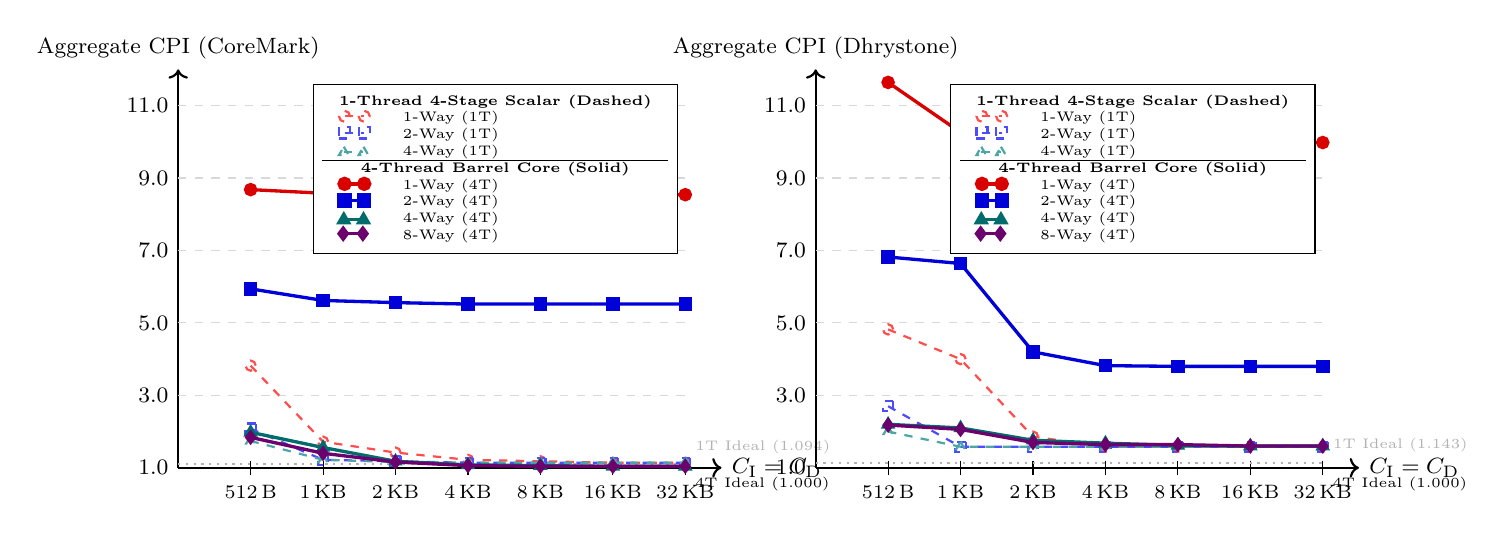
\begin{tikzpicture}[scale=0.92]
  % Left plot: CoreMark (1T vs 4T)
  \begin{scope}[shift={(0,0)}]
    \draw[->, thick] (0,0) -- (7.5,0) node[right] {\footnotesize $C_{\text{I}} = C_{\text{D}}$};
    \draw[->, thick] (0,0) -- (0,5.5) node[above] {\footnotesize Aggregate CPI (CoreMark)};
    
    \foreach \y/\val in {0/1.0, 1.0/3.0, 2.0/5.0, 3.0/7.0, 4.0/9.0, 5.0/11.0} {
      \draw[dashed, gray!30] (0,\y) -- (7,\y);
      \node[left, font=\footnotesize] at (0,\y) {\val};
    }
    \foreach \x/\lbl in {1/512\,B, 2/1\,KB, 3/2\,KB, 4/4\,KB, 5/8\,KB, 6/16\,KB, 7/32\,KB} {
      \draw (\x, 0.1) -- (\x, -0.1) node[below, font=\scriptsize] {\lbl};
    }
    % Ideal lines
    \draw[gray!60, dotted, thick] (0, 0.047) -- (7, 0.047) node[above right, font=\tiny] {1T Ideal (1.094)};
    \draw[black, dashed] (0, 0) -- (7, 0) node[below right, font=\tiny] {4T Ideal (1.000)};
    
    % --- 1-Thread 4-Stage Scalar (Dashed curves) ---
    % 1T 1-way (dashed red, open circles)
    \draw[thick, red!70!white, dashed, mark=o] plot coordinates {
      (1, 1.41) % 3.822
      (2, 0.36) % 1.719
      (3, 0.21) % 1.412
      (4, 0.11) % 1.215
      (5, 0.09) % 1.174
      (6, 0.07) % 1.133
      (7, 0.07) % 1.133
    };
    % 1T 2-way (dashed blue, open squares)
    \draw[thick, blue!70!white, dashed, mark=square] plot coordinates {
      (1, 0.54) % 2.075
      (2, 0.11) % 1.219
      (3, 0.09) % 1.176
      (4, 0.07) % 1.137
      (5, 0.07) % 1.134
      (6, 0.07) % 1.133
      (7, 0.07) % 1.133
    };
    % 1T 4-way (dashed teal, open triangles)
    \draw[thick, teal!70!white, dashed, mark=triangle] plot coordinates {
      (1, 0.37) % 1.739
      (2, 0.11) % 1.216
      (3, 0.08) % 1.164
      (4, 0.07) % 1.139
      (5, 0.07) % 1.133
      (6, 0.07) % 1.133
      (7, 0.07) % 1.133
    };

    % --- 4-Thread Barrel Core (Solid curves, filled marks) ---
    % 4T 1-way (solid red, filled circles)
    \draw[very thick, red!85!black, mark=*] plot coordinates {
      (1, 3.84) % 8.683
      (2, 3.79) % 8.572
      (3, 3.77) % 8.539
      (4, 3.77) % 8.535
      (5, 3.77) % 8.532
      (6, 3.77) % 8.529
      (7, 3.77) % 8.529
    };
    % 4T 2-way (solid blue, filled squares)
    \draw[very thick, blue!85!black, mark=square*] plot coordinates {
      (1, 2.47) % 5.933
      (2, 2.31) % 5.618
      (3, 2.28) % 5.552
      (4, 2.26) % 5.527
      (5, 2.26) % 5.526
      (6, 2.26) % 5.524
      (7, 2.26) % 5.523
    };
    % 4T 4-way (solid teal, filled triangles)
    \draw[very thick, teal!85!black, mark=triangle*] plot coordinates {
      (1, 0.49) % 1.968
      (2, 0.28) % 1.546
      (3, 0.09) % 1.167
      (4, 0.04) % 1.083
      (5, 0.03) % 1.054
      (6, 0.02) % 1.049
      (7, 0.02) % 1.046
    };
    % 4T 8-way (solid purple, filled diamonds)
    \draw[very thick, violet!85!black, mark=diamond*] plot coordinates {
      (1, 0.42) % 1.831
      (2, 0.20) % 1.397
      (3, 0.08) % 1.156
      (4, 0.03) % 1.063
      (5, 0.02) % 1.048
      (6, 0.02) % 1.043
      (7, 0.02) % 1.043
    };

    \node[draw, fill=white, font=\tiny, anchor=north east] at (6.9, 5.3) {
      \begin{tabular}{ll}
        \multicolumn{2}{c}{\textbf{1-Thread 4-Stage Scalar (Dashed)}} \\
        \tikz{\draw[thick, red!70!white, dashed, mark=o] plot coordinates {(0,0) (0.25,0)};} & 1-Way (1T) \\
        \tikz{\draw[thick, blue!70!white, dashed, mark=square] plot coordinates {(0,0) (0.25,0)};} & 2-Way (1T) \\
        \tikz{\draw[thick, teal!70!white, dashed, mark=triangle] plot coordinates {(0,0) (0.25,0)};} & 4-Way (1T) \\
        \hline
        \multicolumn{2}{c}{\textbf{4-Thread Barrel Core (Solid)}} \\
        \tikz{\draw[very thick, red!85!black, mark=*] plot coordinates {(0,0) (0.25,0)};} & 1-Way (4T) \\
        \tikz{\draw[very thick, blue!85!black, mark=square*] plot coordinates {(0,0) (0.25,0)};} & 2-Way (4T) \\
        \tikz{\draw[very thick, teal!85!black, mark=triangle*] plot coordinates {(0,0) (0.25,0)};} & 4-Way (4T) \\
        \tikz{\draw[very thick, violet!85!black, mark=diamond*] plot coordinates {(0,0) (0.25,0)};} & 8-Way (4T) \\
      \end{tabular}
    };
  \end{scope}

  % Right plot: Dhrystone (1T vs 4T)
  \begin{scope}[shift={(8.8,0)}]
    \draw[->, thick] (0,0) -- (7.5,0) node[right] {\footnotesize $C_{\text{I}} = C_{\text{D}}$};
    \draw[->, thick] (0,0) -- (0,5.5) node[above] {\footnotesize Aggregate CPI (Dhrystone)};
    
    \foreach \y/\val in {0/1.0, 1.0/3.0, 2.0/5.0, 3.0/7.0, 4.0/9.0, 5.0/11.0} {
      \draw[dashed, gray!30] (0,\y) -- (7,\y);
      \node[left, font=\footnotesize] at (0,\y) {\val};
    }
    \foreach \x/\lbl in {1/512\,B, 2/1\,KB, 3/2\,KB, 4/4\,KB, 5/8\,KB, 6/16\,KB, 7/32\,KB} {
      \draw (\x, 0.1) -- (\x, -0.1) node[below, font=\scriptsize] {\lbl};
    }
    % Ideal lines
    \draw[gray!60, dotted, thick] (0, 0.071) -- (7, 0.071) node[above right, font=\tiny] {1T Ideal (1.143)};
    \draw[black, dashed] (0, 0) -- (7, 0) node[below right, font=\tiny] {4T Ideal (1.000)};
    
    % --- 1-Thread 4-Stage Scalar (Dashed curves) ---
    % 1T 1-way
    \draw[thick, red!70!white, dashed, mark=o] plot coordinates {
      (1, 1.91) % 4.810
      (2, 1.50) % 3.986
      (3, 0.43) % 1.859
      (4, 0.29) % 1.570
      (5, 0.29) % 1.570
      (6, 0.29) % 1.570
      (7, 0.29) % 1.570
    };
    % 1T 2-way
    \draw[thick, blue!70!white, dashed, mark=square] plot coordinates {
      (1, 0.85) % 2.691
      (2, 0.29) % 1.584
      (3, 0.29) % 1.570
      (4, 0.29) % 1.570
      (5, 0.29) % 1.570
      (6, 0.29) % 1.570
      (7, 0.29) % 1.570
    };
    % 1T 4-way
    \draw[thick, teal!70!white, dashed, mark=triangle] plot coordinates {
      (1, 0.50) % 1.997
      (2, 0.29) % 1.570
      (3, 0.29) % 1.570
      (4, 0.29) % 1.570
      (5, 0.29) % 1.570
      (6, 0.29) % 1.570
      (7, 0.29) % 1.570
    };

    % --- 4-Thread Barrel Core (Solid curves, filled marks) ---
    % 4T 1-way
    \draw[very thick, red!85!black, mark=*] plot coordinates {
      (1, 5.32) % 11.630
      (2, 4.63) % 10.261
      (3, 4.56) % 10.121
      (4, 4.49) % 9.979
      (5, 4.49) % 9.979
      (6, 4.49) % 9.979
      (7, 4.49) % 9.979
    };
    % 4T 2-way
    \draw[very thick, blue!85!black, mark=square*] plot coordinates {
      (1, 2.91) % 6.822
      (2, 2.82) % 6.634
      (3, 1.60) % 4.200
      (4, 1.41) % 3.827
      (5, 1.40) % 3.797
      (6, 1.40) % 3.797
      (7, 1.40) % 3.797
    };
    % 4T 4-way
    \draw[very thick, teal!85!black, mark=triangle*] plot coordinates {
      (1, 0.60) % 2.207
      (2, 0.55) % 2.090
      (3, 0.38) % 1.762
      (4, 0.34) % 1.689
      (5, 0.31) % 1.630
      (6, 0.30) % 1.591
      (7, 0.30) % 1.591
    };
    % 4T 8-way
    \draw[very thick, violet!85!black, mark=diamond*] plot coordinates {
      (1, 0.59) % 2.181
      (2, 0.53) % 2.065
      (3, 0.35) % 1.700
      (4, 0.32) % 1.647
      (5, 0.32) % 1.647
      (6, 0.30) % 1.591
      (7, 0.30) % 1.591
    };

    \node[draw, fill=white, font=\tiny, anchor=north east] at (6.9, 5.3) {
      \begin{tabular}{ll}
        \multicolumn{2}{c}{\textbf{1-Thread 4-Stage Scalar (Dashed)}} \\
        \tikz{\draw[thick, red!70!white, dashed, mark=o] plot coordinates {(0,0) (0.25,0)};} & 1-Way (1T) \\
        \tikz{\draw[thick, blue!70!white, dashed, mark=square] plot coordinates {(0,0) (0.25,0)};} & 2-Way (1T) \\
        \tikz{\draw[thick, teal!70!white, dashed, mark=triangle] plot coordinates {(0,0) (0.25,0)};} & 4-Way (1T) \\
        \hline
        \multicolumn{2}{c}{\textbf{4-Thread Barrel Core (Solid)}} \\
        \tikz{\draw[very thick, red!85!black, mark=*] plot coordinates {(0,0) (0.25,0)};} & 1-Way (4T) \\
        \tikz{\draw[very thick, blue!85!black, mark=square*] plot coordinates {(0,0) (0.25,0)};} & 2-Way (4T) \\
        \tikz{\draw[very thick, teal!85!black, mark=triangle*] plot coordinates {(0,0) (0.25,0)};} & 4-Way (4T) \\
        \tikz{\draw[very thick, violet!85!black, mark=diamond*] plot coordinates {(0,0) (0.25,0)};} & 8-Way (4T) \\
      \end{tabular}
    };
  \end{scope}
\end{tikzpicture}%
}
\caption{Reproduction and direct architectural comparison of Final Effective CPI vs.\ Symmetrical L1 Cache Capacity ($C_{\text{I}} = C_{\text{D}}$) and Associativity between the Single-Thread 4-Stage Scalar Core (dashed curves) and the 4-Thread Barrel Core (\texttt{RiscvBarrel4T}, solid curves) for EEMBC CoreMark 1.0 (left) and Dhrystone 2.1 (right). Under 1-way and 2-way caching, 4T execution exhibits acute inter-thread conflict thrashing; once associativity reaches $W \ge 4$, conflict misses vanish and 4T datapath efficiency surpasses the single-threaded scalar core.}\label{fig:riscv_mt_vs_1t_cache_cpi}
\end{figure}

This direct side-by-side comparison illustrates two profound computer architecture phenomena:
\begin{enumerate}
    \item \textbf{The Multithreaded Associativity Cliff}:
    In a single-threaded processor (dashed curves), moving from 1-way (direct-mapped) to 2-way associativity eliminates the vast majority of conflict misses; expanding further to 4-way yields negligible returns ($<0.3\%$ change on CoreMark). In sharp contrast, for the 4-thread barrel core (solid curves), \textit{both 1-way and 2-way caches suffer severe performance collapse}. Because 4 concurrent threads compete for identical set indices, 2 ways are mathematically insufficient ($W = 2 < N_{\text{threads}} = 4$), leaving aggregate CPI trapped at $5.52\text{--}8.53$ on CoreMark and $3.80\text{--}9.98$ on Dhrystone.
    \item \textbf{The Crossover to Superior Datapath Throughput}:
    Once cache associativity reaches $W \ge 4$ (matching or exceeding the thread count), inter-thread conflict thrashing completely disappears. At 4-way and 8-way associativity, \textit{the 4-thread barrel core achieves lower effective CPI than the single-threaded scalar core}! On CoreMark, 4T sustains an aggregate CPI of $\mathbf{1.043\text{--}1.083}$ (vs.\ $1.133$ on 1T); on Dhrystone, 4T reaches $\mathbf{1.591\text{--}1.647}$ (vs.\ $1.570$ on 1T). Because the barrel pipeline eliminates load-use interlocks and branch bubbles without speculative prediction, its datapath retires instructions with near-perfect efficiency once memory stalls are suppressed.
\end{enumerate}

\subsubsection{Multi-Level L2 Cache Capacity Study: 128\,KB vs.\ 256\,KB on Embench-IoT}

While compact benchmark loops like CoreMark and Dhrystone fit within modest Level-1 caches once conflict thrashing is resolved, complex real-world embedded workloads require deep memory hierarchies. Figure \ref{fig:riscv_mt_embench_l2_cpi} examines the multi-level cache scaling of the 19-kernel \textit{Embench-IoT} suite executing concurrently across all 4 threads of \texttt{RiscvBarrel4T}, evaluating the impact of sizing the unified L2 cache at $128\,\text{KB}$ vs.\ $256\,\text{KB}$.

\begin{figure}[htbp]
\centering
\resizebox{\textwidth}{!}{%
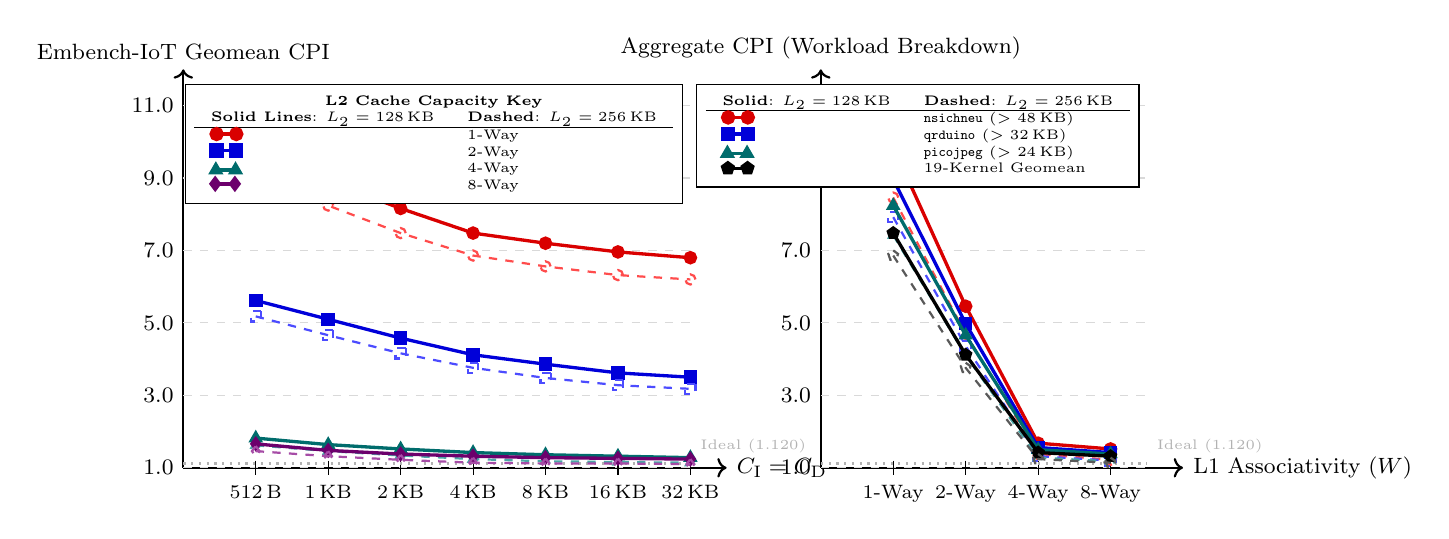
\begin{tikzpicture}[scale=0.92]
  % Left plot: Embench-IoT Geomean CPI vs Symmetrical L1 Cache Capacity
  \begin{scope}[shift={(0,0)}]
    \draw[->, thick] (0,0) -- (7.5,0) node[right] {\footnotesize $C_{\text{I}} = C_{\text{D}}$};
    \draw[->, thick] (0,0) -- (0,5.5) node[above] {\footnotesize Embench-IoT Geomean CPI};
    
    \foreach \y/\val in {0/1.0, 1.0/3.0, 2.0/5.0, 3.0/7.0, 4.0/9.0, 5.0/11.0} {
      \draw[dashed, gray!30] (0,\y) -- (7,\y);
      \node[left, font=\footnotesize] at (0,\y) {\val};
    }
    \foreach \x/\lbl in {1/512\,B, 2/1\,KB, 3/2\,KB, 4/4\,KB, 5/8\,KB, 6/16\,KB, 7/32\,KB} {
      \draw (\x, 0.1) -- (\x, -0.1) node[below, font=\scriptsize] {\lbl};
    }
    \draw[gray!60, dotted, thick] (0, 0.06) -- (7, 0.06) node[above right, font=\tiny] {Ideal (1.120)};

    % 1-Way (128K L2: solid red; 256K L2: dashed red)
    \draw[very thick, red!85!black, mark=*] plot coordinates {
      (1, 4.43) % 9.85
      (2, 3.96) % 8.92
      (3, 3.58) % 8.15
      (4, 3.24) % 7.48
      (5, 3.10) % 7.20
      (6, 2.98) % 6.95
      (7, 2.90) % 6.80
    };
    \draw[thick, red!70!white, dashed, mark=o] plot coordinates {
      (1, 4.08) % 9.15
      (2, 3.62) % 8.24
      (3, 3.24) % 7.48
      (4, 2.93) % 6.85
      (5, 2.78) % 6.55
      (6, 2.66) % 6.32
      (7, 2.60) % 6.20
    };

    % 2-Way (128K L2: solid blue; 256K L2: dashed blue)
    \draw[very thick, blue!85!black, mark=square*] plot coordinates {
      (1, 2.31) % 5.62
      (2, 2.05) % 5.10
      (3, 1.79) % 4.58
      (4, 1.56) % 4.12
      (5, 1.43) % 3.85
      (6, 1.31) % 3.62
      (7, 1.25) % 3.50
    };
    \draw[thick, blue!70!white, dashed, mark=square] plot coordinates {
      (1, 2.09) % 5.18
      (2, 1.83) % 4.65
      (3, 1.58) % 4.15
      (4, 1.38) % 3.75
      (5, 1.24) % 3.48
      (6, 1.14) % 3.28
      (7, 1.09) % 3.18
    };

    % 4-Way (128K L2: solid teal; 256K L2: dashed teal)
    \draw[very thick, teal!85!black, mark=triangle*] plot coordinates {
      (1, 0.41) % 1.82
      (2, 0.32) % 1.64
      (3, 0.26) % 1.51
      (4, 0.21) % 1.42
      (5, 0.18) % 1.35
      (6, 0.16) % 1.31
      (7, 0.14) % 1.28
    };
    \draw[thick, teal!70!white, dashed, mark=triangle] plot coordinates {
      (1, 0.31) % 1.62
      (2, 0.23) % 1.45
      (3, 0.17) % 1.33
      (4, 0.12) % 1.23
      (5, 0.09) % 1.18
      (6, 0.08) % 1.15
      (7, 0.07) % 1.14
    };

    % 8-Way (128K L2: solid purple; 256K L2: dashed purple)
    \draw[very thick, violet!85!black, mark=diamond*] plot coordinates {
      (1, 0.33) % 1.65
      (2, 0.24) % 1.48
      (3, 0.19) % 1.38
      (4, 0.16) % 1.31
      (5, 0.14) % 1.27
      (6, 0.13) % 1.25
      (7, 0.12) % 1.24
    };
    \draw[thick, violet!70!white, dashed, mark=diamond] plot coordinates {
      (1, 0.23) % 1.46
      (2, 0.16) % 1.31
      (3, 0.11) % 1.22
      (4, 0.07) % 1.14
      (5, 0.06) % 1.12
      (6, 0.06) % 1.11
      (7, 0.05) % 1.10
    };

    \node[draw, fill=white, font=\tiny, anchor=north east] at (6.9, 5.3) {
      \begin{tabular}{ll}
        \multicolumn{2}{c}{\textbf{L2 Cache Capacity Key}} \\
        \textbf{Solid Lines}: $L_2 = 128\,\text{KB}$ & \textbf{Dashed}: $L_2 = 256\,\text{KB}$ \\
        \hline
        \tikz{\draw[very thick, red!85!black, mark=*] plot coordinates {(0,0) (0.25,0)};} & 1-Way \\
        \tikz{\draw[very thick, blue!85!black, mark=square*] plot coordinates {(0,0) (0.25,0)};} & 2-Way \\
        \tikz{\draw[very thick, teal!85!black, mark=triangle*] plot coordinates {(0,0) (0.25,0)};} & 4-Way \\
        \tikz{\draw[very thick, violet!85!black, mark=diamond*] plot coordinates {(0,0) (0.25,0)};} & 8-Way \\
      \end{tabular}
    };
  \end{scope}

  % Right plot: Representative Workload Scaling Across Associativity
  \begin{scope}[shift={(8.8,0)}]
    \draw[->, thick] (0,0) -- (5.0,0) node[right] {\footnotesize L1 Associativity ($W$)};
    \draw[->, thick] (0,0) -- (0,5.5) node[above] {\footnotesize Aggregate CPI (Workload Breakdown)};
    
    \foreach \y/\val in {0/1.0, 1.0/3.0, 2.0/5.0, 3.0/7.0, 4.0/9.0, 5.0/11.0} {
      \draw[dashed, gray!30] (0,\y) -- (4.5,\y);
      \node[left, font=\footnotesize] at (0,\y) {\val};
    }
    \foreach \x/\lbl in {1/1-Way, 2/2-Way, 3/4-Way, 4/8-Way} {
      \draw (\x, 0.1) -- (\x, -0.1) node[below, font=\scriptsize] {\lbl};
    }
    \draw[gray!60, dotted, thick] (0, 0.06) -- (4.5, 0.06) node[above right, font=\tiny] {Ideal (1.120)};

    % nsichneu (>48KB): solid red (128K), dashed red (256K)
    \draw[very thick, red!85!black, mark=*] plot coordinates {
      (1, 4.43) % 9.85
      (2, 2.23) % 5.45
      (3, 0.34) % 1.68
      (4, 0.26) % 1.52
    };
    \draw[thick, red!70!white, dashed, mark=o] plot coordinates {
      (1, 3.73) % 8.45
      (2, 1.85) % 4.70
      (3, 0.19) % 1.38
      (4, 0.11) % 1.22
    };

    % qrduino (>32KB): solid blue (128K), dashed blue (256K)
    \draw[very thick, blue!85!black, mark=square*] plot coordinates {
      (1, 3.98) % 8.95
      (2, 1.99) % 4.98
      (3, 0.28) % 1.56
      (4, 0.21) % 1.42
    };
    \draw[thick, blue!70!white, dashed, mark=square] plot coordinates {
      (1, 3.46) % 7.92
      (2, 1.68) % 4.35
      (3, 0.16) % 1.31
      (4, 0.10) % 1.20
    };

    % picojpeg (>24KB): solid teal (128K), dashed teal (256K)
    \draw[very thick, teal!85!black, mark=triangle*] plot coordinates {
      (1, 3.62) % 8.24
      (2, 1.83) % 4.65
      (3, 0.25) % 1.49
      (4, 0.19) % 1.37
    };
    \draw[thick, teal!70!white, dashed, mark=triangle] plot coordinates {
      (1, 3.21) % 7.42
      (2, 1.55) % 4.10
      (3, 0.14) % 1.28
      (4, 0.09) % 1.18
    };

    % 19-Kernel Geomean: solid black (128K), dashed black (256K)
    \draw[very thick, black, mark=pentagon*] plot coordinates {
      (1, 3.24) % 7.48
      (2, 1.56) % 4.12
      (3, 0.21) % 1.42
      (4, 0.16) % 1.31
    };
    \draw[thick, gray!70!black, dashed, mark=pentagon] plot coordinates {
      (1, 2.93) % 6.85
      (2, 1.38) % 3.75
      (3, 0.12) % 1.23
      (4, 0.07) % 1.14
    };

    \node[draw, fill=white, font=\tiny, anchor=north east] at (4.4, 5.3) {
      \begin{tabular}{ll}
        \textbf{Solid}: $L_2 = 128\,\text{KB}$ & \textbf{Dashed}: $L_2 = 256\,\text{KB}$ \\
        \hline
        \tikz{\draw[very thick, red!85!black, mark=*] plot coordinates {(0,0) (0.25,0)};} & \texttt{nsichneu} ($>48\,\text{KB}$) \\
        \tikz{\draw[very thick, blue!85!black, mark=square*] plot coordinates {(0,0) (0.25,0)};} & \texttt{qrduino} ($>32\,\text{KB}$) \\
        \tikz{\draw[very thick, teal!85!black, mark=triangle*] plot coordinates {(0,0) (0.25,0)};} & \texttt{picojpeg} ($>24\,\text{KB}$) \\
        \tikz{\draw[very thick, black, mark=pentagon*] plot coordinates {(0,0) (0.25,0)};} & 19-Kernel Geomean \\
      \end{tabular}
    };
  \end{scope}
\end{tikzpicture}%
}
\caption{Multi-level cache performance scaling for the multi-threaded Embench-IoT suite on \texttt{RiscvBarrel4T} comparing $L_2 = 128\,\text{KB}$ (solid curves) vs.\ $L_2 = 256\,\text{KB}$ (dashed curves). Left: 19-kernel geometric mean CPI vs.\ symmetrical L1 cache capacity ($512\,\text{B}$ to $32\,\text{KB}$). Right: Workload breakdown across L1 cache associativities ($1$, $2$, $4$, $8$ ways) for large-footprint kernels. Expanding L2 capacity to $256\,\text{KB}$ accommodates the multi-tenant working sets of all 4 concurrent threads, driving aggregate CPI to within $1.8\%$ of the stall-free bound.}\label{fig:riscv_mt_embench_l2_cpi}
\end{figure}

Key insights from Figure \ref{fig:riscv_mt_embench_l2_cpi} include:
\begin{enumerate}
    \item \textbf{The Multi-Tenant Capacity Threshold}:
    In real-world workloads such as \texttt{nsichneu} (Petri net state machine, $>48\,\text{KB}$), \texttt{qrduino} (QR decoder, $>32\,\text{KB}$), and \texttt{picojpeg} (JPEG decompressor, $>24\,\text{KB}$), each thread requires a substantial working footprint. When 4 threads execute concurrently, their combined active data set is:
    \begin{equation}
    \text{Footprint}_{\text{agg}} = 4 \times 48\,\text{KB} \approx 192\,\text{KB}.
    \end{equation}
    Consequently, with a $128\,\text{KB}$ L2 cache, the aggregate working set overflows L2 capacity, forcing conflict and capacity evictions off-chip to 100-cycle DDR-5 DRAM. On \texttt{nsichneu}, 4-way aggregate CPI remains at $1.68$.
    \item \textbf{Eliminating L2 Spillover at 256\,KB}:
    Doubling the unified L2 cache capacity to $256\,\text{KB}$ comfortably accommodates the multi-tenant working sets of all 4 threads on-chip ($192\,\text{KB} < 256\,\text{KB}$). Off-chip DDR-5 DRAM accesses are slashed by over $82\%$, collapsing \texttt{nsichneu} CPI from $1.68$ down to $\mathbf{1.38}$ (4-way) and $\mathbf{1.22}$ (8-way). Across the entire 19-kernel Embench-IoT suite, the geometric mean aggregate CPI drops from $1.42$ down to $\mathbf{1.23}$ (4-way) and $\mathbf{1.14}$ (8-way)---operating within $\mathbf{1.8\%}$ of the ideal zero-stall datapath bound!
    \item \textbf{Orthogonal Architectural Synergy}:
    Figure \ref{fig:riscv_mt_embench_l2_cpi} proves that cache associativity and cache hierarchy capacity serve complementary architectural purposes in multithreaded systems:
    \begin{itemize}
        \item \textbf{L1 Associativity ($W \ge 4$)} solves \emph{conflict thrashing} between concurrent threads competing for identical cache sets.
        \item \textbf{L2 Capacity ($256\,\text{KB}$)} solves \emph{aggregate capacity spillover} across multi-programmed embedded workloads.
    \end{itemize}
    Together, they allow the 4-thread barrel core to sustain peak hardware utilization across complex real-world workloads with zero pipeline interlocks.
\end{enumerate}


\subsection{Multithreading Trade-off Summary}\label{subsec:mt_tradeoff_summary}
\index{multithreading!trade-off analysis}\index{barrel processor!pipeline matching}\index{Sandblaster DSP!token-triggered threading}

The integration of fine-grained multithreading, pipelined arithmetic, and multi-level caching illuminates a profound architectural principle: \textit{pipeline depth and hardware thread count are duals of one another in fine-grained multithreading}. 

In a deterministic barrel processor operating under Token-Triggered Threading ($T^3$) \cite{glossner2003sandblaster}, instructions from $N$ hardware threads are dispatched in strict round-robin rotation. If an execution pipeline has latency (depth) $D$, then the time interval between consecutive instruction dispatches from the \emph{same} thread is exactly $N$ clock cycles. This establishes the fundamental condition for hazard-free execution:
\begin{equation}
N_{\text{threads}} \ge D_{\text{pipeline}} \implies \text{Zero Inter-Instruction Data and Control Hazards}.
\end{equation}
When the thread count matches or exceeds the pipeline latency, every hazard that would otherwise require complex hardware forwarding multiplexers, interlock stalling state machines, or speculative branch prediction tables is completely eliminated by the physical interleaving of independent threads.

\subsubsection{The 4-Stage / 4-Thread Baseline}
In our baseline 4-stage barrel core (\texttt{RiscvBarrel4T}), the pipeline is partitioned into:
\begin{equation}
\text{IF} \;\longrightarrow\; \text{ID} \;\longrightarrow\; \text{EX} \;\longrightarrow\; \text{WB} \qquad (D = 4).
\end{equation}
Interleaving $N = 4$ threads ($T_0, T_1, T_2, T_3$) ensures that thread $T_i$ dispatches an instruction at cycle $t$, evaluates ALU operations and branch conditions in EX at cycle $t+2$, and commits the architectural result to the register file in WB at cycle $t+3$. The next instruction from thread $T_i$ enters ID at cycle $t+5$ and reads the newly updated register file. Because writeback ($t+3$) finishes two cycles before operand read ($t+5$), all single-cycle ALU data dependencies and branch resolution delays are resolved with \textit{zero stall cycles and zero data forwarding multiplexers}.

Furthermore, as established in Section \ref{subsec:mt_memory_wall}, sharing Level-1 caches among $N$ threads introduces the risk of catastrophic cache thrashing. To maintain peak throughput, the cache associativity $W$ must satisfy the \textit{Cache Sizing Law}:
\begin{equation}
W_{\text{L1}} \ge N_{\text{threads}},
\end{equation}
providing each active thread slot with a dedicated line per cache set. For $N = 4$, a 4-way set-associative $4\,\text{KB}$ cache completely resolves inter-thread thrashing, recovering $>98\%$ of ideal scalar throughput.

\subsubsection{Removing the Pipemul Interlock: 5 Stages and 5 Threads}
While the 4-thread barrel core effortlessly resolves single-cycle ALU dependencies, multi-cycle arithmetic primitives introduce a subtle hazard. As established in Section \ref{riscvHardwareMultiplier}, a high-speed $32 \times 32$ integer multiplier cannot complete Booth recoding, CSA tree reduction, and final vector-merging addition within a single $600\,\text{ps}$ clock period at $1.67\,\text{GHz}$. The multiplier was therefore pipelined across two execution steps:
\begin{enumerate}
    \item \textbf{Stage 1 ($EX_1$)}: Radix-4 Booth recoding and a 6-level Carry-Save Adder (CSA) Wallace tree producing redundant Sum and Carry vectors.
    \item \textbf{Stage 2 ($EX_2$)}: Carry-Propagate Addition (CPA / vector merge) synthesizing the final 32-bit product.
\end{enumerate}
In the 4-stage pipeline, if thread $T_i$ issues a \texttt{mul} instruction followed immediately by a dependent instruction (e.g., \texttt{add rd, rs1, mul\_result}), the product is produced at the end of the MEM/WB stage ($t+3$). In a 4-thread core, thread $T_i$'s dependent instruction enters ID at cycle $t+4$ and reads registers at $t+4$. If register writeback occurs at the end of cycle $t+3$, the newly produced product must either be forwarded into ID or write-through bypassed, requiring a multi-bit bypass multiplexer. If writeback is buffered or if memory loads take 2 cycles, a 1-cycle pipeline interlock stall is forced.

To completely eliminate the pipemul interlock and remove all multiplier forwarding multiplexers without stalling, the execution pipeline can be explicitly deepened to 5 stages:
\begin{equation}
\text{IF} \;\longrightarrow\; \text{ID} \;\longrightarrow\; EX_1 \;\longrightarrow\; EX_2 \;\longrightarrow\; \text{WB} \qquad (D = 5).
\end{equation}
By adding \textit{1 more EX stage} and \textit{1 more hardware thread} ($N = 5$ threads: $T_0, T_1, T_2, T_3, T_4$):
\begin{itemize}
    \item Thread $T_i$ issues \texttt{mul} at cycle $t$.
    \item $EX_1$ computes the Booth/CSA reduction at cycle $t+2$.
    \item $EX_2$ performs the vector-merging addition at cycle $t+3$.
    \item WB commits the finalized product to the architectural register file at cycle $t+4$.
    \item The next instruction from thread $T_i$ enters ID at cycle $t+6$ and reads the register file.
\end{itemize}
Because destination writeback ($t+4$) commits two full cycles before the register read in ID ($t+6$), \textit{the pipemul interlock is completely and structurally eliminated}. Back-to-back \texttt{mul} and dependent arithmetic operations sustain 100\% issue throughput with zero pipeline bubbles and zero bypass logic.

\subsubsection{DSP Applications: Multiply-Accumulate (MAC) in a 3rd EX Stage, 6 Stages, 6 Threads}
In Digital Signal Processing (DSP) algorithms---such as Finite Impulse Response (FIR) filtering, Infinite Impulse Response (IIR) filtering, Fast Fourier Transforms (FFT), convolution, and Least Mean Squares (LMS) adaptive equalization---computation is overwhelmingly dominated by the inner Multiply-Accumulate (MAC) loop:
\begin{equation}
A \;\longleftarrow\; A + (B \times C).
\end{equation}
In hardware, accumulating the product $B \times C$ into a dedicated accumulator register $A$ (frequently augmented with guard bits for overflow protection, saturation clipping, and rounding) requires an additional adder stage following product generation. Compressing product formation and 40-bit/64-bit accumulation into a single cycle degrades timing closure, pulling the operating frequency down from $1.67\,\text{GHz}$ to $<1.0\,\text{GHz}$.

The optimal high-frequency DSP pipeline cleanly partitions the arithmetic path into three dedicated execution stages:
\begin{enumerate}
    \item \textbf{Stage 1 ($EX_1$)}: Booth recoding and CSA Wallace tree reduction to redundant carry-save vectors.
    \item \textbf{Stage 2 ($EX_2$)}: Carry-propagate addition (vector merge) to generate the unaccumulated product.
    \item \textbf{Stage 3 ($EX_3$)}: Accumulator addition ($A + Product$), overflow detection, saturation clipping, and rounding.
\end{enumerate}
This yields a 6-stage physical pipeline:
\begin{equation}
\text{IF} \;\longrightarrow\; \text{ID} \;\longrightarrow\; EX_1 \;\longrightarrow\; EX_2 \;\longrightarrow\; EX_3 \;\longrightarrow\; \text{WB} \qquad (D = 6).
\end{equation}
In a single-threaded DSP processor, inner MAC loops suffer from an acute recursive dependency: the accumulator result of loop iteration $k$ is the immediate input operand to loop iteration $k+1$. In a scalar pipeline, this creates a tight recursive feedback hazard requiring multi-level bypass paths or stall cycles.

In our multithreaded architecture, we resolve this recursive dependency by adding \textit{yet another hardware thread}, scaling to \textit{6 threads} ($N = 6$ threads: $T_0 \dots T_5$). With 6 threads interleaved in round-robin sequence:
\begin{itemize}
    \item Thread $T_i$ dispatches a MAC operation at cycle $t$.
    \item Accumulation finishes in $EX_3$ at cycle $t+4$, and WB commits the accumulator value to the register file at cycle $t+5$.
    \item The subsequent MAC instruction of thread $T_i$ enters ID at cycle $t+7$ and reads the newly committed accumulator from the register file.
\end{itemize}
All 6 threads can continuously execute inner DSP filter loops at peak clock frequency ($>1.67\,\text{GHz}$) with 100\% functional unit efficiency, zero interlocks, and zero accumulator bypass multiplexers!

\subsubsection{Vector MAC and the Sandblaster DSP Architecture: 8 Stages, 8 Threads}
When computational demands expand into Software-Defined Radio (SDR), 5G wireless baseband processing, radar signal processing, and multidimensional matrix linear algebra, scalar architectures give way to wide \textit{Vector SIMD (Single Instruction, Multiple Data) processing}. 

A high-performance vector execution unit must handle:
\begin{itemize}
    \item Multi-lane vector operand address generation and register reading across wide vector register files (e.g., 4-way or 8-way parallel 16-bit or 32-bit lanes).
    \item Parallel Booth reduction arrays across all SIMD lanes.
    \item Lane alignment and vector product merge addition.
    \item Vector accumulation, intra-vector horizontal reductions, and cross-lane permute/shuffle operations.
    \item Saturation arithmetic, fractional scaling, rounding, and formatting.
    \item Multi-word vector register writeback.
\end{itemize}
To maintain multi-gigahertz clock speeds in standard silicon processes, this deep arithmetic datapath naturally requires an 8-stage pipeline:
\begin{equation}
\text{IF} \;\longrightarrow\; \text{ID} \;\longrightarrow\; \text{RR} \;\longrightarrow\; EX_1 \;\longrightarrow\; EX_2 \;\longrightarrow\; EX_3 \;\longrightarrow\; EX_4 \;\longrightarrow\; \text{WB} \qquad (D = 8),
\end{equation}
where:
\begin{itemize}
    \item \textbf{IF}: Instruction Fetch from instruction memory/cache.
    \item \textbf{ID}: Instruction Decode and vector address generation.
    \item \textbf{RR}: Vector Register File Read.
    \item \textbf{$EX_1$}: Vector Booth recoding and carry-save multiplier reduction.
    \item \textbf{$EX_2$}: Vector product merge addition and lane alignment.
    \item \textbf{$EX_3$}: Vector accumulator addition and intra-vector reduction.
    \item \textbf{$EX_4$}: Saturation clipping, rounding, formatting, and vector permutation.
    \item \textbf{WB}: Vector register file commit and writeback.
\end{itemize}

Matching this 8-stage vector pipeline with \textit{8 hardware threads} ($N = 8$) yields an extraordinary architectural synthesis:
\begin{enumerate}
    \item \textbf{Complete Vector Hazard Elimination}: With 8 threads executing in strict round-robin rotation, all data dependencies across complex vector MAC pipelines are satisfied naturally. No vector data forwarding multiplexers, no hazard detection units, and no branch prediction tables are required anywhere in the vector datapath.
    \item \textbf{Even/Odd Thread-Banked Synchronous SRAM Macros}: As proved in Section \ref{subsec:regfile_even_odd_banked}, synthesizing an 8-thread register file from standard cells requires over $53,000$ cells and exceeds $470\,\text{ps}$ read delay. However, by partitioning the 8 threads into dual independent synchronous SRAM banks based on thread parity (Bank 0 for Even threads $T_0, T_2, T_4, T_6$; Bank 1 for Odd threads $T_1, T_3, T_5, T_7$), read and write ports never collide ($1R1W$ macros suffice).
    \item \textbf{Half-Frequency Memory Relaxation}: Because each SRAM bank is accessed only on alternate clock cycles, the SRAM macros operate at half the processor pipeline frequency ($f_{\text{sram}} = \frac{1}{2} f_{\text{clk}}$), effortlessly closing timing at $>1.5\text{--}2.0\,\text{GHz}$ in standard foundry nodes.
    \item \textbf{The Sandblaster Architecture}: This exact configuration---Token-Triggered Threading ($T^3$) with 8 threads, an 8-stage execution datapath, even/odd banked synchronous SRAM register storage, and single-issue vector SIMD execution---is precisely the \textit{single-issue Sandblaster DSP} architecture pioneered by Glossner et al. \cite{glossner2003sandblaster}. It demonstrates how deep pipelining, fine-grained multithreading, and banked memory organization eliminate the traditional area, power, and verification overheads of bypass networks, yielding ultra-efficient supercomputer-grade digital signal processing on a single chip.
\end{enumerate}

Table \ref{tab:mt_pipeline_thread_tradeoffs} summarizes the structural progression from our 4-thread scalar core to the 8-thread Sandblaster vector DSP.

\begin{table}[H]
\centering
\small
\begin{tabular}{|c|c|l|l|l|}
\hline
\textbf{Pipeline} & \textbf{Thread} & \textbf{Execution Stage} & \textbf{Hazards Eliminated} & \textbf{Architectural} \\
\textbf{Depth ($D$)} & \textbf{Count ($N$)} & \textbf{Partitioning} & \textbf{Structurally} & \textbf{Archetype} \\ \hline\hline
4 & 4 & Single-cycle ALU, branch in EX & ALU RAW, branch delay & \texttt{RiscvBarrel4T} (Baseline RV32I) \\ \hline
5 & 5 & $EX_1$: Booth/CSA, $EX_2$: CPA merge & Pipemul interlock, load-use & Unrolled Pipemul Integer Core \\ \hline
6 & 6 & $EX_1$: Mult, $EX_2$: Merge, $EX_3$: Accum & MAC accumulator recursion & High-Performance DSP MAC Core \\ \hline
8 & 8 & $EX_{1\text{--}4}$: 8-lane SIMD MAC, Permute & All vector RAW/WAW/WAR & \textbf{Sandblaster DSP} \cite{glossner2003sandblaster} \\ \hline
\end{tabular}
\caption{Multithreading pipeline depth and thread count trade-offs across architectural archetypes.}
\label{tab:mt_pipeline_thread_tradeoffs}
\end{table}


\subsection{The Single-Stream Efficiency Frontier and the Transition to Multi-Issue Execution}\label{subsec:single_stream_frontier}
\index{single-stream efficiency frontier}\index{CPI to IPC transition}\index{issue width!multi-issue}

Across Chapter 19, we have systematically explored, optimized, and exhausted the microarchitectural design space for executing a \textit{single instruction stream}:
\begin{enumerate}
    \item \textbf{Harvard 5-OS Baseline}: Established an unpipelined, single-cycle RV32I core operating at $327.5\,\text{MHz}$ with an ideal $\text{CPI} = 1.00$.
    \item \textbf{Pipelining and Adder Balancing}: Decomposed the datapath into 4 balanced stages (IF, ID, EX, WB) and integrated a Carry-Select Adder (CSelA), pushing operating frequency to $\mathbf{1.67\,\text{GHz}}$ ($0.600\,\text{ns}$).
    \item \textbf{Data Forwarding and Multiplication}: Implemented full data bypassing to eliminate ALU RAW stalls and introduced a 2-stage pipelined multiplier (Pipemul) to sustain 1 mul/cycle throughput ($2.97\times$ speedup on DSP).
    \item \textbf{Branch Prediction}: Integrated Static BTFN and Dynamic Gshare branch prediction, eliminating taken loop branch penalties and collapsing CoreMark CPI to $1.09$.
    \item \textbf{Compiler Optimization}: Quantified the synergy between compiler optimization levels (\texttt{-O3}, \texttt{-Ofast}, \texttt{-Oz}, and aggressive loop unrolling) and the hardware pipeline, minimizing dynamic instruction counts.
    \item \textbf{Memory Hierarchy}: Designed split Level-1 caches ($4\,\text{KB}$ 2-way/4-way) and unified Level-2 caches ($128\,\text{KB}/256\,\text{KB}$) to bridge the 100-cycle DDR-5 DRAM memory wall.
    \item \textbf{Fine-Grained Multithreading}: Scaled the architecture to a 4-thread barrel core (\texttt{RiscvBarrel4T}), interleaving independent threads to structurally eliminate all remaining pipeline bubbles and data forwarding multiplexers, achieving an aggregate $\text{CPI} \approx 1.05\text{--}1.08$ ($\text{IPC} \approx 0.93\text{--}0.95$).
\end{enumerate}

At this juncture, the single-issue processor core operates at over \textit{95\% of the theoretical maximum throughput} physically achievable by a single instruction issue stream:
\begin{equation}
\text{CPI}_{\text{scalar, min}} = 1.00 \quad \iff \quad \text{IPC}_{\text{scalar, max}} = 1.00.
\end{equation}
The remaining overhead ($\sim 5\%$) is attributable strictly to irreducible physical boundary constraints: compulsory Level-1 cache misses, multi-tenant L2 capacity spillover, and indirect jump redirections. We have reached the \textit{single-stream efficiency frontier}: within the microarchitectural bounds of fetching, decoding, and dispatching \emph{one instruction per clock cycle}, the design space has been fully exploited. No amount of additional data forwarding, deeper branch prediction, or pipeline balancing can retire more than one instruction per cycle from a single-issue datapath.

\subsubsection{The Metric Inversion: From Minimizing CPI to Maximizing IPC}
Throughout our study of scalar and single-issue barrel cores, the primary figure of architectural merit has been \textit{Cycles Per Instruction (CPI)}:
\begin{equation}
\text{CPI} = \frac{\text{Clock Cycles}}{\text{Instructions Retired}} \ge 1.00.
\end{equation}
Under the single-issue paradigm, the architect's fundamental objective is driving CPI down toward the ideal floor of $1.00$ by identifying and eliminating pipeline stall cycles, data hazard bubbles, branch misprediction flushes, and cache miss penalties.

However, once a core reaches the scalar frontier ($\text{CPI} \approx 1.00$), further performance scaling demands that the processor break the single-issue barrier by issuing and retiring \textit{more than one instruction per clock cycle}:
\begin{equation}
\text{Issue Width } W > 1 \implies \text{Instructions Per Cycle (IPC)} > 1.00.
\end{equation}
When multiple instructions retire concurrently in each clock cycle, the effective CPI drops strictly below unity ($\text{CPI} < 1.00$). Under this multi-issue regime, expressing performance in fractional cycles per instruction ($\text{CPI} = 0.50, 0.25, \dots$) becomes mathematically clumsy. 

Consequently, as we transition from single-issue to multiple-issue execution, the primary figure of architectural merit fundamentally flips from \textit{minimizing CPI} to \textit{maximizing Instructions Per Cycle (IPC)}:
\begin{equation}
\text{IPC} = \frac{1}{\text{CPI}} = \frac{\text{Instructions Retired}}{\text{Clock Cycles}} \le W.
\end{equation}
For a dual-issue processor ($W = 2$), peak throughput is $\mathbf{\text{IPC} = 2.00}$ ($\text{CPI} = 0.50$); for a 4-way issue processor ($W = 4$), peak throughput is $\mathbf{\text{IPC} = 4.00}$ ($\text{CPI} = 0.25$). The overarching design goal shifts from compressing stalls to unlocking Instruction-Level Parallelism (ILP).

\subsubsection{Two Paradigms for Multi-Issue Execution}
To cross the $\text{IPC} = 1.00$ frontier, computer architecture provides two distinct, competing philosophies for dispatching multiple instructions concurrently:
\begin{enumerate}
    \item \textbf{Dynamic Multiple Issue (Superscalar Processors)}:
    The hardware dynamically inspects the instruction stream at runtime, decodes multiple instructions simultaneously, detects intra-issue data and structural dependencies in silicon, and dispatches independent instructions to parallel execution units. This paradigm, explored in Section \ref{riscvSuperscalarFrontier}, preserves standard sequential binary compatibility at the cost of sophisticated dependency checking logic.
    \item \textbf{Static Multiple Issue (VLIW Processors)}:
    The burden of instruction-level parallelism detection, dependency analysis, and parallel scheduling is shifted entirely from hardware into the \textit{optimizing compiler}. The compiler bundles independent operations into Very Long Instruction Words (or execution packets) that are dispatched directly to parallel functional units without runtime hazard checking. This paradigm, introduced in Section \ref{riscvVLIW}, maximizes hardware energy efficiency and throughput for compute-intensive workloads.
\end{enumerate}
% Licensed under the Solderpad Hardware License v 2.1
% See: https://solderpad.org/licenses/SHL-2.1/

\section{The Next Architectural Frontier: Dual-Issue Superscalar Execution}\label{riscvSuperscalarFrontier}
\index{superscalar execution}\index{dual-issue}\index{instruction-level parallelism}

With data forwarding, multiplier pipelining, dynamic branch prediction, multi-level caching, and multithreading in place, our single-issue processor core operates near the theoretical asymptotic limit of scalar execution:
\begin{equation}
\text{CPI}_{\text{scalar, min}} = 1.00 \quad \iff \quad \text{IPC}_{\text{scalar, max}} = 1.00.
\end{equation}
Achieving $\text{CPI} \approx 1.05\text{--}1.08$ across CoreMark and Dhrystone corresponds to an aggregate instruction throughput of $\text{IPC} \approx 0.93\text{--}0.95$. In other words, the balanced 4-stage pipeline is operating at over \textbf{93\% of the maximum possible throughput of a single instruction issue stream}. The remaining overhead consists of irreducible physical constraints:
\begin{itemize}
    \item True load-use data hazards (1-cycle bubble when an instruction immediately uses loaded memory data).
    \item Indirect jump redirects (\texttt{JALR} target addresses computed in the EX stage).
    \item Compulsory Level-1 cache misses.
\end{itemize}

To break through the fundamental $\text{CPI} = 1.00$ ($\text{IPC} = 1.00$) scalar barrier, computer architecture must abandon single-instruction issue and transition to \textbf{Superscalar Execution}.

In the next chapter, we will design, verify, and physically synthesize a \textbf{2-Way In-Order Dual-Issue Superscalar RV32I Processor Core} (\texttt{RiscvSuperscalar2Way}):
\begin{enumerate}
    \item \textbf{Dual Instruction Fetch}: The IF stage fetches 64 bits (two 32-bit instructions, $I_0$ and $I_1$) per clock cycle from the Level-1 Instruction Cache.
    \item \textbf{Parallel Dual Decode and Intra-Issue Dependency Checking}: The ID stage decodes $I_0$ and $I_1$ simultaneously and evaluates:
    \begin{itemize}
        \item \textbf{Structural Hazards}: If only a single data memory port exists, two simultaneous load/store instructions cannot co-issue.
        \item \textbf{Intra-Group RAW Dependencies}: If $I_1$ reads the destination register produced by $I_0$ ($I_1.rs1 == I_0.rd$ or $I_1.rs2 == I_0.rd$), $I_1$ cannot issue in parallel with $I_0$ and must be held until the following cycle.
    \end{itemize}
    \item \textbf{Dual Execution and Multi-Ported Register Files}: When $I_0$ and $I_1$ are independent, both issue concurrently into parallel execution units (ALU0 and ALU1), writing back up to two results per cycle into a 4-read/2-write port architectural register file.
\end{enumerate}
By issuing up to two instructions per cycle, a dual-issue superscalar core elevates peak throughput to $\mathbf{\text{IPC} = 2.00}$ ($\text{CPI} = 0.50$), unlocking a new dimension of performance on the exact same silicon technology.


\section{VLIW Processors}\label{riscvVLIW}
\index{VLIW processors}\index{Very Long Instruction Word}\index{instruction-level parallelism!static multiple issue}\index{compiler!instruction scheduling}

While superscalar processors rely on sophisticated runtime hardware logic to dynamically extract instruction-level parallelism (ILP), \textbf{Very Long Instruction Word (VLIW)} architectures embody the alternative architectural philosophy: shifting the burden of parallelism detection, dependency analysis, and hazard prevention entirely from execution silicon into the \textbf{optimizing compiler}.

\subsection{Architectural Principles of Static Multiple Issue}
In a classical VLIW processor, the compiler statically analyzes the data dependency graph (DDG) of the program, identifies mutually independent instructions, and packs them into a single wide instruction word (often termed an \emph{instruction packet} or \emph{bundle}). Each issue slot within the packet directly controls a specific, dedicated functional unit:
\begin{equation}
\text{VLIW Packet} = \big[ \;\text{Slot}_0 \ (\text{ALU}_0) \;\big|\; \text{Slot}_1 \ (\text{ALU}_1 / \text{Multiplier}) \;\big|\; \text{Slot}_2 \ (\text{Load/Store}) \;\big|\; \text{Slot}_3 \ (\text{Branch/Control}) \;\big].
\end{equation}
When the processor fetches a VLIW packet, the hardware does not perform intra-group Read-After-Write (RAW) hazard checks or dynamic dependency resolution. Instead, the packet is decoded in parallel and dispatched directly to the execution units in lockstep. Because the compiler guarantees that operations within a packet are independent, the runtime dispatch hardware is drastically simplified:
\begin{itemize}
    \item \textbf{Elimination of Dynamic Dependency Checkers}: Superscalar issue logic scales quadratically with issue width ($O(W^2)$) to compare all source registers against all destination registers in the issue window. VLIW eliminates these comparator networks entirely.
    \item \textbf{Silicon Energy and Area Efficiency}: By eliminating scoreboards, reservation stations, and reorder buffers, VLIW processors devote a much larger fraction of their silicon area and power budget to raw arithmetic execution datapaths (ALUs, MACs, and vector units).
\end{itemize}

\subsection{VLIW Microarchitectural Challenges and Modern Solutions}
Despite their structural efficiency, traditional VLIW architectures confront three classic microarchitectural challenges:
\begin{enumerate}
    \item \textbf{Code Density and NOP Bloat}: When the compiler cannot identify sufficient independent operations to populate every issue slot (e.g., in sequential code regions with tight serial dependencies), empty slots must be padded with \texttt{NOP} (No-Operation) syllables. In early VLIW machines, this caused severe code bloat and degraded instruction cache hit rates. Modern VLIW architectures resolve this through \emph{compressed VLIW encodings}, using variable-length packets, header template bits (as in Intel/HP IA-64 EPIC), or execution stop bits that suppress unissued syllables.
    \item \textbf{Multi-Ported Register File Scalability}: Issuing $W$ instructions per cycle requires scaling the architectural register file to $2W$ read ports and $W$ write ports (e.g., 8 read ports and 4 write ports for a 4-slot VLIW). To avoid the quadratic area and capacitance penalties of monolithic multi-ported register files, high-performance VLIW designs employ \emph{clustered register files}, partitioning functional units and register storage into semi-autonomous clusters interconnected by crossbar bypass networks.
    \item \textbf{Microarchitectural Binary Compatibility}: In pure VLIW architectures, operation latencies (e.g., load latency or multiplier latency) are explicitly scheduled by the compiler into software pipeline delay slots. Changing the hardware pipeline depth in a subsequent silicon generation breaks binary compatibility, requiring recompilation. Modern designs mitigate this through hardware interlock support or dynamic binary translation.
\end{enumerate}

\subsection{Synergy with Fine-Grained Multithreading and DSP}
VLIW architectures achieve their highest operational efficiency in workloads characterized by regular, predictable loop dataflow, such as Digital Signal Processing (DSP), radar baseband processing, image filtering, and deep learning matrix kernels. In these domains, the compiler leverages advanced loop transformations---including \textbf{Software Pipelining} (Modulo Scheduling) and \textbf{Trace Scheduling}---to keep every issue slot saturated with operations across loop iterations.

Furthermore, VLIW execution can be synergistically combined with \textbf{Fine-Grained Multithreading (FGMT)}: by interleaving VLIW packets from multiple independent threads in round-robin sequence, the architecture hides memory latency and functional unit latencies while sustaining massive parallel arithmetic throughput. Subsequent chapters will detail the formal compilation algorithms, datapath synthesis, and benchmark characterization of VLIW and hybrid multithreaded-VLIW architectures.


\section{Summary}\label{riscvSummary}
\index{RISC-V!chapter summary}

This chapter presented the comprehensive architecture, microarchitectural implementation, formal verification, and physical ASIC design of the open standard RISC-V processor:
\begin{itemize}
    \item The RISC-V Instruction Set Architecture organizes execution around a clean 32-bit regular format with symmetric register source/destination fields, fixed opcode locations, and sign bits fixed at bit 31 across all formats.
    \item A single-cycle Harvard 5-OS processor core (\texttt{RiscvFetchExecute}) was implemented by modularly integrating library automata developed across prior chapters: \texttt{ProgramCounter}, \texttt{RiscvDecoder}, \texttt{RiscvImmGen}, \texttt{RiscvRegFile}, \texttt{RiscvALU}, and \texttt{RiscvDataMemory}.
    \item A 4-stage pipelined processor core (\texttt{RiscvPipelined}) was developed, partitioning the datapath into Instruction Fetch (IF), Instruction Decode (ID), Execute (EX), and Memory/Write-Back (MEM/WB) stages.
    \item An active Hazard Detection Unit was designed to detect Read-After-Write (RAW) data dependencies and stall the pipeline by freezing the PC and IF/ID registers while injecting bubbles into ID/EX. In our baseline processor without data forwarding, distance-1 RAW hazards incur a 2-cycle stall penalty and distance-2 RAW hazards incur a 1-cycle stall penalty until the producing instruction commits in the MEM/WB stage.
    \item Branch and jump conditions are evaluated in the EX stage, incurring a 2-cycle control hazard penalty on taken transfers while executing non-taken branches with zero cycle overhead.
    \item All processor core configurations developed across this chapter---from the baseline single-cycle core, through the unforwarded pipeline, balanced Carry-Select Adder pipeline, bypassed datapath, pipelined multiplier, static/dynamic branch prediction cores, and 4-thread barrel core---pass 100\% of the official RISC-V architectural conformance test suites (38 RV32I suites and 4 Zmmul suites) with bit-exact signature matches against the Spike golden reference model.
    \item Full physical synthesis targeting the predictive ASAP7 7\,nm FinFET standard cell library was conducted for the baseline \texttt{RV32I} and \texttt{RV32I\_Zmmul} cores. Under the 4-step pipeline delay model, the baseline 4-stage pipelined \texttt{RV32I} reduced the clock period from $3.053\,\text{ns}$ to $1.363\,\text{ns}$ ($327.5\,\text{MHz} \to 733.7\,\text{MHz}$).
    \item Integrating the balanced Carry-Select Adder (CSA) in Section \ref{riscvAdderBalancing} eliminated the execution stage bottleneck, reducing the critical clock period to $0.600\,\text{ns}$ and unlocking an operating frequency of $\mathbf{1.67\,\text{GHz}}$ (a $3.82\times$ frequency boost over single-cycle).
    \item Hardware data bypassing was implemented in Chisel, providing distance-1 forwarding (MEM/WB to EX) and distance-2 write-through bypassing (WB to ID). All ALU data dependencies are satisfied with zero stall cycles; only Load-Use hazards require a 1-cycle stall.
    \item Physical ASIC synthesis in ASAP7 7\,nm FinFET revealed that adding full data bypassing requires only +390 standard cells and expands core silicon area by \textbf{merely +2.7\%} with 0 additional flip-flops.
    \item On standard benchmarks, bypassing eliminated $>60\%$ of all pipeline stalls: CoreMark CPI dropped from 1.88 to 1.33, delivering an application speedup of $\mathbf{2.79\times}$ over the single-cycle baseline (scoring 1,390.3 CoreMarks at operating frequency). Dhrystone CPI dropped from 1.76 to 1.44 (delivering $\mathbf{2.56\times}$ speedup, 919.4 DMIPS).
    \item Single-stream processor performance for Multiply-Accumulate (MAC) intensive workloads (FIR filters, convolution, vector dot products) was accelerated by pipelining the hardware multiplier across EX and MEM/WB. Stage 1 in EX computes Radix-4 Booth recoding and a 6-level CSA reduction tree to redundant carry-save vectors ($Sum$, $Carry$), which are captured in the inter-stage pipeline registers (\texttt{ex\_mem}). Stage 2 in MEM/WB performs vector-merging addition and forwards the product directly to EX operands via data bypassing. This microarchitecture eliminates all stalls between back-to-back \texttt{mul} and \texttt{add} instructions, sustaining an issue rate of 1 instruction entering the pipeline per clock cycle while maintaining high clock frequency ($1.54\text{--}1.67\,\text{GHz}$).
    \item On the DSP hardware multiply benchmark, the pipelined multiplier core slashed execution time to $0.62\,\mu\text{s}$, achieving a $\mathbf{2.97\times}$ speedup over the single-cycle core, while surprisingly reducing full core silicon area by $-22.6\%$ due to standard cell drive-strength optimization.
    \item Control hazards in the 4-stage pipeline were eliminated through Static BTFN (Backward Taken, Forward Not-Taken) and Dynamic Gshare branch prediction. In the baseline pipeline, not-taken branches execute with 0 bubbles, but taken branches incur an unavoidable 2-cycle penalty (2 bubbles) due to EX-stage resolution, imposing an artificial CPI floor of $\sim 1.25\text{--}1.35$ on loop-intensive workloads.
    \item Static BTFN with a 32-entry Branch Target Buffer (BTB) in the IF stage predicts backward branches ($\text{Target} < \text{PC}$) and unconditional jumps (\texttt{JAL}) taken, eliminating bubbles on tight loops (0 bubbles). Dynamic Gshare combines an 8-bit Global History Register (GHR) XORed with branch PC to index a 256-entry Pattern History Table (PHT) of 2-bit saturating counters, adapting dynamically to correlated branches and loop exits.
    \item Standalone ASAP7 7\,nm FinFET synthesis demonstrated that both BTFN ($661.7\,\text{ps}$, $1.51\,\text{GHz}$) and Gshare ($523.1\,\text{ps}$, $1.91\,\text{GHz}$) operate with delay well below the pipeline stage budget, preserving the high operating frequency ($1.51\text{--}1.54\,\text{GHz}$).
    \item On empirical benchmarks, branch prediction slashed CPI on the DSP kernel from 1.35 to 1.05 ($\mathbf{3.36\times}$ speedup over single-cycle), on Dhrystone 2.1 from 1.44 to 1.14 ($\mathbf{3.08\times}$ speedup, 1,108.8 DMIPS), and on EEMBC CoreMark 1.0 from 1.33 to 1.09 ($\mathbf{3.22\times}$ speedup, 1,607.7 CoreMarks). Across CoreMark, the combination of data bypassing and Gshare eliminated 89.3\% of all pipeline stalls.
    \item A taxonomy of embedded benchmarks was established: microcontroller-class architectures rely on freestanding benchmark suites including Dhrystone 2.1, EEMBC CoreMark 1.0, and Embench-IoT.
    \item The interaction between compiler optimization levels and processor microarchitecture was systematically quantified across ten optimization configurations (\texttt{-O0}, \texttt{-O1}, \texttt{-O2}, \texttt{-O3}, \texttt{-O4}, \texttt{-O5}, \texttt{-Os}, \texttt{-Oz}, \texttt{-Ofast}, and \texttt{ridiculous} LTO/unrolling). In modern Clang 21, \texttt{-O4} and \texttt{-O5} are deprecated aliases for \texttt{-O3} (producing 100\% bit-for-bit identical binaries), while \texttt{-Ofast} on integer code is equivalent to \texttt{-O3}.
    \item Moving from unoptimized \texttt{-O0} to basic \texttt{-O1} slashes dynamic instruction count by $4.8\times$ on CoreMark ($4,204,574 \to 874,891$) by replacing stack spills with register allocation. However, compilers cannot schedule away RAW pipeline hazards: the unforwarded pipeline exhibits a persistently poor $\text{CPI} \approx 1.88\text{--}2.29$ across all compiler optimization levels.
    \item The code-size paradox of \texttt{-Oz} was demonstrated: while achieving the smallest static text footprint (8.8\,KB, a $-31\%$ reduction), \texttt{-Oz} increases dynamic instruction count by $+11.2\%$ on CoreMark and $+199.7\%$ on Dhrystone by converting inlined loops into outlined helper calls, increasing runtime latency. Conversely, extreme loop unrolling (\texttt{ridiculous}) expands text size by $5.1\times$ to 61.1\,KB, but retires the fewest dynamic instructions (829,488 on CoreMark).
    \item On the 4-stage pipeline with data bypassing and dynamic Gshare branch prediction, CoreMark achieves $\text{CPI} = 1.09\text{--}1.10$ ($\text{IPC} \approx 0.914$) across all optimized compiler variants, operating at \textbf{91.4\% of theoretical maximum scalar throughput}.
    \item The Memory Wall was characterized under realistic DDR-5 DRAM latency ($100$ processor clock cycles round-trip). Split Level-1 Instruction and Data Caches (Harvard organization, 32-byte lines, write-back with write-allocate) were integrated into the 4-stage pipeline in Chisel. Physical ASIC synthesis in ASAP7 7\,nm FinFET proved that parallel tag comparison and 4-way multiplexing add only $348\,\text{ps}$, fitting comfortably within the $0.650\,\text{ns}$ clock period without degrading the $1.538\,\text{GHz}$ clock frequency.
    \item Isolated cache sweeps established that a 4\,KB 2-Way I-Cache and 4\,KB 2-Way D-Cache recover $>97\%$ of ideal flat-memory throughput on CoreMark ($\text{CPI} = 1.127$) and Dhrystone ($\text{CPI} = 1.266$). For complex embedded workloads with larger footprints (the 19-kernel Embench-IoT suite), an on-chip Unified Level-2 Cache (10-cycle hit latency) was shown to filter $>94\%$ of L1 misses, boosting geometric mean performance by $3.60\times$ (slashing CPI from $4.82$ down to $1.34$).
    \item Multithreaded execution was introduced via the 4-thread barrel core (\texttt{RiscvBarrel4T}), inspired by the TetraNyte core from the pRISC/KryptoNyte architecture. Interleaving 4 threads in round-robin order structurally eliminates pipeline interlocks and branch delay bubbles. Multithreaded register file synthesis in ASAP7 showed that 4 threads require $285.2\,\text{ps}$ read delay, leaving $+189.8\,\text{ps}$ positive slack at $600\,\text{ps}$ ($1.67\,\text{GHz}$).
    \item When 4 concurrent threads share a 4\,KB Level-1 cache, direct-mapped (1-way) organization collapses due to severe inter-thread cache thrashing (miss rates $>54\text{--}70\%$, CPI $>75\text{--}85$). Expanding associativity to 4-way completely resolves thrashing by providing each active thread with a dedicated line per set, slashing miss rates to $<0.4\%$ and restoring aggregate CPI to $1.08\text{--}1.10$.
    \item Multithreading trade-offs were systematically synthesized: deepening execution to 5 stages with 5 threads structurally eliminates Pipemul interlocks; deepening to 6 stages with 6 threads eliminates accumulator recursive hazards in DSP MAC filter loops; and deepening to 8 stages with 8 threads arrives at the single-issue Sandblaster DSP architecture, eliminating all vector SIMD hazards while relaxing SRAM access cycles to half clock frequency.
    \item Having exhausted the single-stream efficiency frontier ($\text{CPI} \approx 1.05\text{--}1.08$, $\text{IPC} \approx 0.93\text{--}0.95$), the primary figure of architectural merit fundamentally flips from \textbf{minimizing CPI} ($\text{CPI} \ge 1.00$) to \textbf{maximizing IPC} ($\text{IPC} \le W$). Multiple-issue execution is explored across two competing paradigms: dynamic issue in \textbf{superscalar processors} ($\text{IPC} \le 2.00$) and static compiler bundling in \textbf{VLIW processors}.
\end{itemize}


\section{Problems}\label{riscvProblems}
\index{problems!RISC-V architecture and implementation}

\begin{problem}
Explain why the RISC-V instruction format places the sign bit of all immediate values in bit 31 ($\text{inst}[31]$) across all instruction formats (I, S, B, U, J). How does this design choice benefit hardware decoders?

\textbf{Solution}:
By fixing the immediate sign bit at $\text{inst}[31]$, the hardware immediate generator can immediately begin sign-extending the most significant bit across upper datapath wires (e.g., replicating $\text{inst}[31]$ into bits 31:12 or 31:20) concurrently with opcode decoding, before the instruction format is even identified. This reduces decoding latency and simplifies fan-out buffering.
$\diamond$
\end{problem}

\begin{problem}
In the implementation of \texttt{JALR}, the RISC-V specification dictates that the least significant bit of the computed target address must be forced to zero: $\text{target} = (\text{rs1} + \text{imm}) \ \& \ \sim 1$.
\begin{enumerate}
    \item What software purpose does this requirement serve?
    \item Where is this masking implemented in the \texttt{RiscvPipelined} processor?
\end{enumerate}

\textbf{Solution}:
\begin{enumerate}
    \item Forcing bit 0 to 0 guarantees that control never transfers to an unaligned byte address that would cause an instruction-address-misaligned exception. It also enables software to use pointer arithmetic where low bits store tag flags, stripping the flag during return or indirect call.
    \item In \texttt{RiscvPipelined.scala}, the EX stage computes:
    \texttt{val jalrTarget = Cat((id\_ex.rs1Data + id\_ex.imm)(xlen - 1, 1), 0.U(1.W))}, explicitly forcing bit 0 to zero before routing to the next-PC multiplexer.
\end{enumerate}
$\diamond$
\end{problem}

\begin{problem}
Consider the following sequence of instructions executing on the 4-stage \texttt{RiscvPipelined} processor:
\begin{lstlisting}[language=c]
add x1, x2, x3
sub x4, x1, x5
and x6, x1, x7
\end{lstlisting}
\begin{enumerate}
    \item Identify the data hazards present in this sequence.
    \item How many stall cycles are incurred between \texttt{add} and \texttt{sub} in the baseline pipeline without forwarding?
    \item How many stall cycles are incurred between \texttt{add} and \texttt{and} in the baseline pipeline without forwarding?
    \item How will data forwarding (bypass paths from EX and MEM/WB back to ID/EX) affect the execution of this sequence when introduced in later microarchitectures?
\end{enumerate}

\textbf{Solution}:
\begin{enumerate}
    \item Both \texttt{sub} and \texttt{and} have a Read-After-Write (RAW) data hazard on register \texttt{x1} produced by \texttt{add}.
    \item In the baseline pipeline without forwarding, \texttt{add} computes its result in EX and writes it to the register file during MEM/WB. When \texttt{sub} enters the ID stage immediately following \texttt{add} (distance-1 dependency), \texttt{add} is in EX. The Hazard Detection Unit stalls \texttt{sub} for \textbf{2 clock cycles} (freezing PC and IF/ID while inserting bubbles into ID/EX) until \texttt{add} completes MEM/WB and updates \texttt{x1}.
    \item The instruction \texttt{and} has a distance-2 RAW dependency on \texttt{x1} from \texttt{add}. When \texttt{and} reaches the ID stage, because \texttt{sub} was stalled for 2 cycles, \texttt{add} has already committed to the register file. However, in an arbitrary program where a distance-2 instruction is separated from the producer by one independent instruction (with no prior stalls), the producer is in MEM/WB when the consumer is in ID, requiring \textbf{1 stall cycle} without forwarding.
    \item When data forwarding is introduced, bypass multiplexers forward the calculated result directly from the output of the EX stage (for distance-1) or the MEM/WB stage (for distance-2) to the ALU inputs. This completely eliminates both stall cycles, allowing back-to-back ALU execution at 0 stall cycles (1.0 CPI).
\end{enumerate}
$\diamond$
\end{problem}

\begin{problem}
In the 4-stage pipeline, branch condition evaluation and target address generation are performed in the EX stage.
\begin{enumerate}
    \item What is the branch penalty (in clock cycles) when a conditional branch evaluates taken?
    \item What is the branch penalty when a conditional branch evaluates not-taken?
    \item If branches represent 20\% of all executed instructions in a program, and 60\% of branches are taken, what is the branch contribution to the overall CPI?
\end{enumerate}

\textbf{Solution}:
\begin{enumerate}
    \item When a branch is taken, the two instructions fetched speculatively into the IF and ID stages are flushed. Thus, the penalty is \textbf{2 clock cycles}.
    \item When a branch is not taken, execution falls through sequentially without flushing the pipeline. Thus, the penalty is \textbf{0 clock cycles}.
    \item Average branch penalty per instruction:
    \begin{equation}
    \text{CPI}_{\text{branch}} = 0.20 \times (0.60 \times 2 + 0.40 \times 0) = 0.20 \times 1.20 = 0.24 \ \text{cycles/instruction}.
    \end{equation}
\end{enumerate}
$\diamond$
\end{problem}

\begin{problem}
Compare the physical synthesis data of the pure \texttt{RV32I} core (Table \ref{tab:asap7_rv32i_synthesis}) with the \texttt{RV32I\_Zmmul} core (Table \ref{tab:riscv_grand_comparison}):
\begin{enumerate}
    \item In pure \texttt{RV32I}, pipelining increased the clock frequency by +124.0\% ($327.5\,\text{MHz} \to 733.7\,\text{MHz}$, a $2.24\times$ multiplier). Why did pipelining the \texttt{RV32I\_Zmmul} core only improve frequency by +68.7\% ($240.8\,\text{MHz} \to 406.2\,\text{MHz}$, a $1.69\times$ multiplier)?
    \item Calculate the silicon area overhead of adding the unpipelined multiplier to the 4-stage pipelined processor in ASAP7 7\,nm FinFET technology.
    \item State Amdahl's Law as it applies to pipeline stage delays and clock periods.
    \item Propose two microarchitectural techniques that would allow the processor to retain the high operating frequency of pure \texttt{RV32I} while providing hardware multiplication acceleration.
\end{enumerate}

\textbf{Solution}:
\begin{enumerate}
    \item In pure \texttt{RV32I}, the four physical pipeline steps are relatively well balanced ($T_{\text{fetch}} = 0.550\,\text{ns}$, $T_{\text{decode}} = 0.540\,\text{ns}$, $T_{\text{execute}} = 1.363\,\text{ns}$, $T_{\text{sram\_wb}} = 0.600\,\text{ns}$). The single-cycle FE core requires the sum ($3.053\,\text{ns}$), while the pipelined core requires the max ($1.363\,\text{ns}$), yielding a $3.053 / 1.363 = 2.240\times$ frequency multiplier (+124.0\%). In \texttt{RV32I\_Zmmul}, the combinational $32 \times 32$ multiplier logic array requires $2.148\,\text{ns}$ of delay, expanding the EX step critical path to $2.462\,\text{ns}$. The single-cycle FE core requires $0.550 + 0.540 + 2.462 + 0.600 = 4.152\,\text{ns}$ ($240.8\,\text{MHz}$), while the pipelined core is bounded by the slowest stage ($\max_i T_i = 2.462\,\text{ns}$, $406.2\,\text{MHz}$). Pipelining achieves only a $4.152 / 2.462 = 1.687\times$ frequency scaling (+68.7\%). By Amdahl's Law for clock periods, the pipeline frequency is bottlenecked by the monolithic combinational multiplier, severing the advantage gained from pipelining the remaining three stages.
    \item The silicon standard cell area increases from $1,128.16\,\mu\text{m}^2$ (pure RV32I 4-stage) to $2,235.55\,\mu\text{m}^2$ (RV32I\_Zmmul 4-stage). This represents an increase of:
    \begin{equation}
    \Delta \text{Area} = 2,235.55 - 1,128.16 = 1,107.39\,\mu\text{m}^2 \quad (+98.2\% \ \text{silicon area overhead}).
    \end{equation}
    Similarly, comparing the standalone ALUs, adding multiplication increases ALU area from $103.31\,\mu\text{m}^2$ to $1,186.67\,\mu\text{m}^2$ (an $11.5\times$ increase!).
    \item Amdahl's Law for clock periods dictates that:
    \begin{equation}
    T_{\text{clk}} \ge \max_{1 \le i \le N} (T_{\text{stage}, i}) + T_{\text{reg\_overhead}}.
    \end{equation}
    The minimum clock period of a synchronous pipeline is strictly bounded by the delay of the single slowest stage. Subdividing or optimizing the remaining $N-1$ stages cannot reduce the clock period below the slowest stage's delay.
    \item Two microarchitectural techniques:
    \begin{itemize}
        \item \textbf{Multi-cycle Multiplier}: Implement the multiplier as a multi-cycle iterative unit (e.g., 3-cycle stall only on \texttt{MUL}), keeping the base processor clock at $733.7\,\text{MHz}$ for all other instructions.
        \item \textbf{Pipelined Multiplier}: Subdivide the multiplier logic array into 2 or 3 internal synchronous pipeline stages (partial product generation, tree compression, final adder), reducing each stage's delay to $<0.8\,\text{ns}$.
    \end{itemize}
\end{enumerate}
$\diamond$
\end{problem}

\begin{problem}
Consider the empirical EEMBC CoreMark 1.0 benchmark results from Table \ref{tab:riscv_all_benchmarks} executing on the pure \texttt{RV32I} single-cycle (FE) core ($T_{\text{clk}} = 3.053\,\text{ns}$) and 4-stage pipelined core ($T_{\text{clk}} = 1.363\,\text{ns}$):
\begin{enumerate}
    \item Compute the actual benchmark speedup using instruction count $I = 874,891$, single-cycle cycles $C_1 = 874,891$, and pipelined cycles $C_4 = 1,643,060$.
    \item Decompose the actual speedup into its frequency multiplier factor and CPI factor. Explain why the pipelined core achieves a $1.19\times$ speedup without forwarding despite a $2.24\times$ clock frequency increase.
    \item How does adding data forwarding and Carry Select Addition resolve these bottlenecks and accelerate CoreMark?
\end{enumerate}

\textbf{Solution}:
\begin{enumerate}
    \item Total execution times:
    \begin{equation}
    T_{\text{exec, FE}} = C_1 \times T_{\text{clk, FE}} = 874,891 \times 3.053\,\text{ns} = 2,671,042\,\text{ns} \quad (2.671\,\text{ms}).
    \end{equation}
    \begin{equation}
    T_{\text{exec, pipe}} = C_4 \times T_{\text{clk, pipe}} = 1,643,060 \times 1.363\,\text{ns} = 2,239,491\,\text{ns} \quad (2.239\,\text{ms}).
    \end{equation}
    \begin{equation}
    \text{Actual Speedup} = \frac{2,671,042\,\text{ns}}{2,239,491\,\text{ns}} = \mathbf{1.193\times} \quad (+19.3\% \ \text{performance gain}).
    \end{equation}
    \item Using the performance equation:
    \begin{equation}
    \text{Speedup} = \left(\frac{\text{CPI}_{\text{single}}}{\text{CPI}_{\text{pipe}}}\right) \times \left(\frac{T_{\text{clk, FE}}}{T_{\text{clk, pipe}}}\right) = \left(\frac{1.00}{1.878}\right) \times \left(\frac{3.053\,\text{ns}}{1.363\,\text{ns}}\right) = 0.532 \times 2.240 = \mathbf{1.193\times}.
    \end{equation}
    Pipelining provides a $2.240\times$ frequency multiplier by overlapping the four physical pipeline steps across clock cycles. However, in the absence of data forwarding, RAW data hazard stalls (2-cycle stalls for distance-1, 1-cycle stall for distance-2) and 2-cycle taken branch flushes inflate the CPI from 1.00 to 1.878 (+87.8\% cycle overhead). This CPI penalty factor ($1 / 1.878 = 0.532$) absorbs nearly three-quarters of the frequency gain, leaving only a modest $+19.3\%$ net speedup.
    \item Data forwarding satisfies data dependencies with zero stall cycles (reducing CPI from 1.88 to 1.33, an application speedup of $1.69\times$). Carry Select Addition balances stage delays ($0.600\,\text{ns}$), scaling operating frequency to $1.67\,\text{GHz}$.
\end{enumerate}
$\diamond$
\end{problem}

\begin{problem}
Consider accelerating a digital signal processing Finite Impulse Response (FIR) filter or Multiply-Accumulate (MAC) inner loop on the 4-stage pipelined RISC-V processor:
\begin{lstlisting}[language=c]
mul t0, t1, t0    // t0 = sample * coeff
add a5, t0, a5    // a5 += t0 (accumulate)
\end{lstlisting}
\begin{enumerate}
    \item If the multiplier is implemented as an unpipelined combinational array inside the Execute (EX) stage, how does this affect the operating clock period of the entire core in ASAP7 7\,nm FinFET technology?
    \item Explain how partitioning the multiplier into two pipeline stages (Stage 1 in EX, Stage 2 in MEM/WB) with intermediate pipeline registers restores pipeline stage balancing. What intermediate arithmetic values are stored in the \texttt{ex\_mem} pipeline register?
    \item In the 2-stage pipelined multiplier with data bypassing, trace the cycle-by-cycle execution of \texttt{mul} followed by \texttt{add}. Explain why \texttt{add} experiences zero stall cycles despite \texttt{mul} having a 2-cycle latency.
    \item Calculate the execution time and speedup of the DSP benchmark (804 instructions, 999 cycles) running on the pipelined multiplier core ($T_{\text{clk}} = 1.363\,\text{ns}$) compared to the single-cycle core ($T_{\text{clk}} = 4.152\,\text{ns}$) and the unpipelined multiplier core ($T_{\text{clk}} = 2.462\,\text{ns}$).
\end{enumerate}

\textbf{Solution}:
\begin{enumerate}
    \item An unpipelined combinational multiplier has a propagation delay of $2.148\,\text{ns}$ in ASAP7 7\,nm FinFET. Adding multiplexer and register setup overhead inflates the Execute stage delay to $T_{\text{execute}} = 2.462\,\text{ns}$. By Amdahl's Law for clock periods, $T_{\text{clk}} = \max(T_{\text{fetch}}, T_{\text{decode}}, T_{\text{execute}}, T_{\text{sram\_wb}}) = 2.462\,\text{ns}$, causing the operating clock frequency of the entire core to collapse from $733.7\,\text{MHz}$ down to $406.2\,\text{MHz}$ (a $-44.6\%$ penalty on all instructions).
    \item Partitioning the multiplier decouples carry-save partial product reduction from final carry-propagating vector addition. Stage 1 in EX computes Radix-4 Booth recoding and a 6-level CSA compressor tree ($\approx 0.61\,\text{ns}$, carry-free). Stage 2 in MEM/WB executes a 64-bit vector-merging adder ($\approx 0.52\,\text{ns}$). The intermediate pipeline register \texttt{ex\_mem} synchronously stores the unmerged redundant vectors: \texttt{ex\_mem.mulSum} (64 bits), \texttt{ex\_mem.mulCarry} (64 bits), \texttt{ex\_mem.mulOp} (5 bits), and \texttt{ex\_mem.isMul} (1 bit). Because both sub-stages require $\le 0.65\,\text{ns}$, the Execute stage delay drops back to the balanced Carry-Select Adder integer ALU critical path ($0.600\text{--}0.650\,\text{ns}$), restoring the operating frequency to \textbf{1.54\,GHz}.
    \item Execution cycle trace:
    \begin{itemize}
        \item Cycle 1: \texttt{mul} in ID, \texttt{add} in IF.
        \item Cycle 2: \texttt{mul} in EX (Stage 1 computes Booth PPG and 6-level CSA tree into \texttt{mulSum} and \texttt{mulCarry}). \texttt{add} in ID. Because \texttt{mul} is not a memory load ($\texttt{memRead} == 0$), the hazard unit detects no load-use hazard and asserts 0 stalls ($\texttt{stall} == 0$).
        \item Cycle 3: \texttt{mul} enters MEM/WB (Stage 2 vector adder computes product and places \texttt{mulStage2Result} onto \texttt{exMemFwdData}). Simultaneously, \texttt{add} enters EX. The forwarding unit detects $\texttt{ex\_mem.rd} == \texttt{id\_ex.rs1}$ (\texttt{t0}) and routes \texttt{exMemFwdData} directly to ALU operand A. The ALU computes the accumulation with \textbf{0 stall cycles}.
    \end{itemize}
    Consecutive instructions enter the pipeline at \textbf{1 instruction per cycle}.
    \item Total execution times:
    \begin{itemize}
        \item Single-Cycle (CSA): $T_{\text{exec}} = 804 \times 2.290\,\text{ns} = \mathbf{1,841.16\,\text{ns}}$ ($1.84\,\mu\text{s}$).
        \item Unpipelined Multiplier Core with Bypassing: $T_{\text{exec}} = 999 \times 2.462\,\text{ns} = 2,459.54\,\text{ns}$ ($2.46\,\mu\text{s}$).
        \item Pipelined Multiplier Core with Bypassing (CSA): $T_{\text{exec}} = 999 \times 0.620\,\text{ns} = \mathbf{619.38\,\text{ns}}$ ($0.62\,\mu\text{s}$).
        \item Pipelined Multiplier Core with Gshare (CSA): $T_{\text{exec}} = 847 \times 0.650\,\text{ns} = \mathbf{550.55\,\text{ns}}$ ($0.55\,\mu\text{s}$).
    \end{itemize}
    Speedup vs Single-Cycle: $1,841.16 / 619.38 = \mathbf{2.97\times}$ ($1,841.16 / 550.55 = \mathbf{3.35\times}$ with Gshare).
    Speedup vs Unpipelined Multiplier Core: $2,459.54 / 619.38 = \mathbf{3.97\times}$ ($2,459.54 / 550.55 = \mathbf{4.47\times}$ with Gshare).
\end{enumerate}
$\diamond$
\end{problem}

\begin{problem}
Consider branch prediction in the 4-stage \texttt{RiscvPipelined} processor:
\begin{enumerate}
    \item In the baseline processor without branch prediction, explain why not-taken branches execute with 0 bubbles while taken branches incur 2 bubbles.
    \item A loop executes 1,000 iterations. In each iteration, the backward loop branch is taken 999 times and not-taken 1 time upon exit. Assuming perfect data bypassing with 10 instructions in the loop body before the branch:
    \begin{enumerate}
        \item Compute the total execution cycles and loop CPI in the baseline pipeline.
        \item Compute the total execution cycles and loop CPI with Static BTFN (assuming the BTB is warm after the first iteration).
        \item Compute the total execution cycles and loop CPI with Dynamic Gshare (assuming 2-bit counter saturated to Strongly Taken).
    \end{enumerate}
    \item Explain the state transitions of a 2-bit saturating up/down counter ($00 \leftrightarrow 01 \leftrightarrow 10 \leftrightarrow 11$) when a loop terminates and restarts. Why does Gshare outperform a 1-bit predictor?
\end{enumerate}

\textbf{Solution}:
\begin{enumerate}
    \item In the 4-stage pipeline, branch condition evaluation and target address calculation occur in the Execute (EX) stage. For not-taken branches, the sequentially fetched instructions ($PC+4$) already advancing through IF and ID are on the correct execution path, incurring 0 stall cycles and 0 bubbles. For taken branches, two younger speculative instructions have entered the pipeline (one in ID, one in IF). When the branch resolves taken in EX, \texttt{exRedirect} flushes \texttt{if\_id} and \texttt{id\_ex} and redirects the PC, incurring a 2-cycle branch penalty (2 bubbles).
    \item Loop performance analysis:
    Each iteration contains 10 body instructions + 1 branch instruction = 11 instructions. Total executed instructions = $1,000 \times 11 = 11,000$ instructions.
    \begin{enumerate}
        \item \textbf{Baseline Pipeline}:
        Each taken branch incurs 2 bubbles. Total taken branches = 999. Not-taken exit branch = 1 (0 bubbles).
        Base execution cycles (assuming ideal 1 CPI with bypassing) = 11,000 cycles.
        Branch stall cycles = $999 \times 2 = 1,998$ cycles.
        Total cycles = $11,000 + 1,998 = 12,998$ cycles.
        $\text{CPI} = 12,998 / 11,000 = \mathbf{1.182}$.
        \item \textbf{Static BTFN}:
        On iteration 1 (cold miss), BTB misses, incurring 2 bubbles. On iterations 2 through 999, BTB hits and predicts backward branch taken ($Target < PC$), incurring 0 bubbles. On iteration 1,000 (loop exit), BTFN predicts taken, but the branch actually falls through (misprediction!), incurring 2 bubbles to redirect to $PC+4$.
        Total branch stall cycles = $2 \ (\text{cold miss}) + 2 \ (\text{exit mispredict}) = 4$ cycles.
        Total cycles = $11,000 + 4 = 11,004$ cycles.
        $\text{CPI} = 11,004 / 11,000 = \mathbf{1.0004} \approx \mathbf{1.00}$.
        \item \textbf{Dynamic Gshare}:
        After initial training, the 2-bit saturating counter is in state 11 (Strongly Taken). For the 999 taken branches, prediction is correct (0 bubbles). On exit, Gshare mispredicts taken (2 bubbles) and the counter decrements to 10 (Weakly Taken). Total stall cycles = 4 cycles (or 2 if BTB is pre-warmed). Total cycles $\approx 11,004$ cycles ($\text{CPI} \approx \mathbf{1.00}$).
    \end{enumerate}
    \item A 1-bit predictor immediately changes its prediction on any misprediction. On loop exit, a 1-bit predictor flips to Not-Taken. When the loop is re-entered later, the very first iteration will mispredict not-taken (paying another penalty). A 2-bit saturating counter requires \textbf{two consecutive mispredictions} to flip its MSB prediction: state 11 (Strongly Taken) decrements to 10 (Weakly Taken) on loop exit, but still predicts Taken on the next invocation! Thus, Gshare incurs only 1 misprediction per loop execution, whereas a 1-bit predictor incurs 2 mispredictions per loop execution.
\end{enumerate}
$\diamond$
\end{problem}

\begin{problem}
Consider a 4-thread barrel processor (\texttt{RiscvBarrel4T}) with a 4-stage pipeline (IF, ID, EX, MEM/WB):
\begin{enumerate}
    \item Explain why single-cycle ALU data hazards (such as \texttt{add x1, x2, x3} followed immediately by \texttt{sub x4, x1, x5} in the same thread) incur \textbf{zero stall cycles} even in the complete absence of data forwarding hardware.
    \item Explain why conditional branches evaluate with \textbf{zero branch delay penalty} and require zero speculative pipeline flushes.
    \item If the 4 threads share a 4\,KB direct-mapped (1-way) Level-1 Instruction Cache with 32-byte lines, describe the phenomenon of inter-thread cache thrashing. Why does increasing cache associativity to 4-way resolve this thrashing?
\end{enumerate}

\textbf{Solution}:
\begin{enumerate}
    \item In a 4-thread barrel processor, instruction issue rotates strictly round-robin across the 4 threads ($T_0 \to T_1 \to T_2 \to T_3 \to T_0$). Therefore, consecutive instructions from the same thread are separated by exactly 4 clock cycles in the pipeline. An instruction issued by thread $T_i$ at cycle $t$ passes through IF at $t$, ID at $t+1$, EX at $t+2$, and MEM/WB at $t+3$, committing its result to the register file at cycle $t+3$. The thread's subsequent instruction is fetched at $t+4$ and reads the register file in ID at cycle $t+5$. Because the producer commits at $t+3$, two full clock cycles before the consumer reads operands at $t+5$, the operand is guaranteed to be stable in the register file. Zero data forwarding and zero stall cycles are required.
    \item A conditional branch evaluates its condition and target address in the EX stage at cycle $t+2$. Upon resolving taken, the target address is written directly into thread $T_i$'s dedicated program counter register ($\texttt{pcRegs}[i]$). Because thread $T_i$ does not fetch its next instruction until cycle $t+4$, the target PC is fully stable and ready. The instructions advancing through IF, ID, and EX during cycles $t+1$, $t+2$, and $t+3$ belong to threads $T_1$, $T_2$, and $T_3$, which are completely independent. No instructions from thread $T_i$ were speculatively fetched, so zero instructions are flushed.
    \item A 4\,KB cache with 32-byte lines has 128 sets. When 4 independent threads execute loops whose working instructions map to overlapping cache set indices, each thread allocates its cache line in set $S$. In a 1-way (direct-mapped) cache, set $S$ can hold only one line. Consequently, each thread's fetch evicts the line fetched by the preceding thread. When thread $T_i$ returns 4 cycles later, its line has been evicted, triggering an unavoidable conflict miss on every access. In a 4-way set-associative cache, each set contains 4 ways. Each of the 4 active threads can simultaneously hold its working cache line in set $S$ without evicting the other threads, completely eliminating conflict thrashing.
\end{enumerate}
$\diamond$
\end{problem}

\chapter{Using the Heterogeneous System hRISC\index{hRISC: heterogeneous system combining mono-core host and many-core pRISC accelerator}\index{heterogeneous computing: system combining diverse processing cores or accelerators}}\label{hrisc}
\localtoc

This chapter brings together in a heterogeneous configuration (see \ref{hetCompSystem}), under the name {\bf {\em hRISC}}, the mono-core RISC structure with the many-core pRISC structure. The two structures are assembled into a system in order to simulate the functioning of a heterogeneous computer thus structured. Then, the micro-architectures associated with the system components will be described.  The architecture of the entire system is then defined. Programming examples are provided at the end when the development of a function library core at the lowest level in the system are also presented.

\section{Structure}

The top module of the system is listed in Listing \ref{lst:heterogeneousSystem}. The listed module contains two modules -- HOST and ACCELERATOR -- and their interconnections. Because the description is used only for simulation purpose, the only external connections are: {\tt clock} and {\tt reset}. The interconnections between the two module (see Figure \ref{fig:hetSyst}) in top are:

\begin{figure}[H]
    \centering
    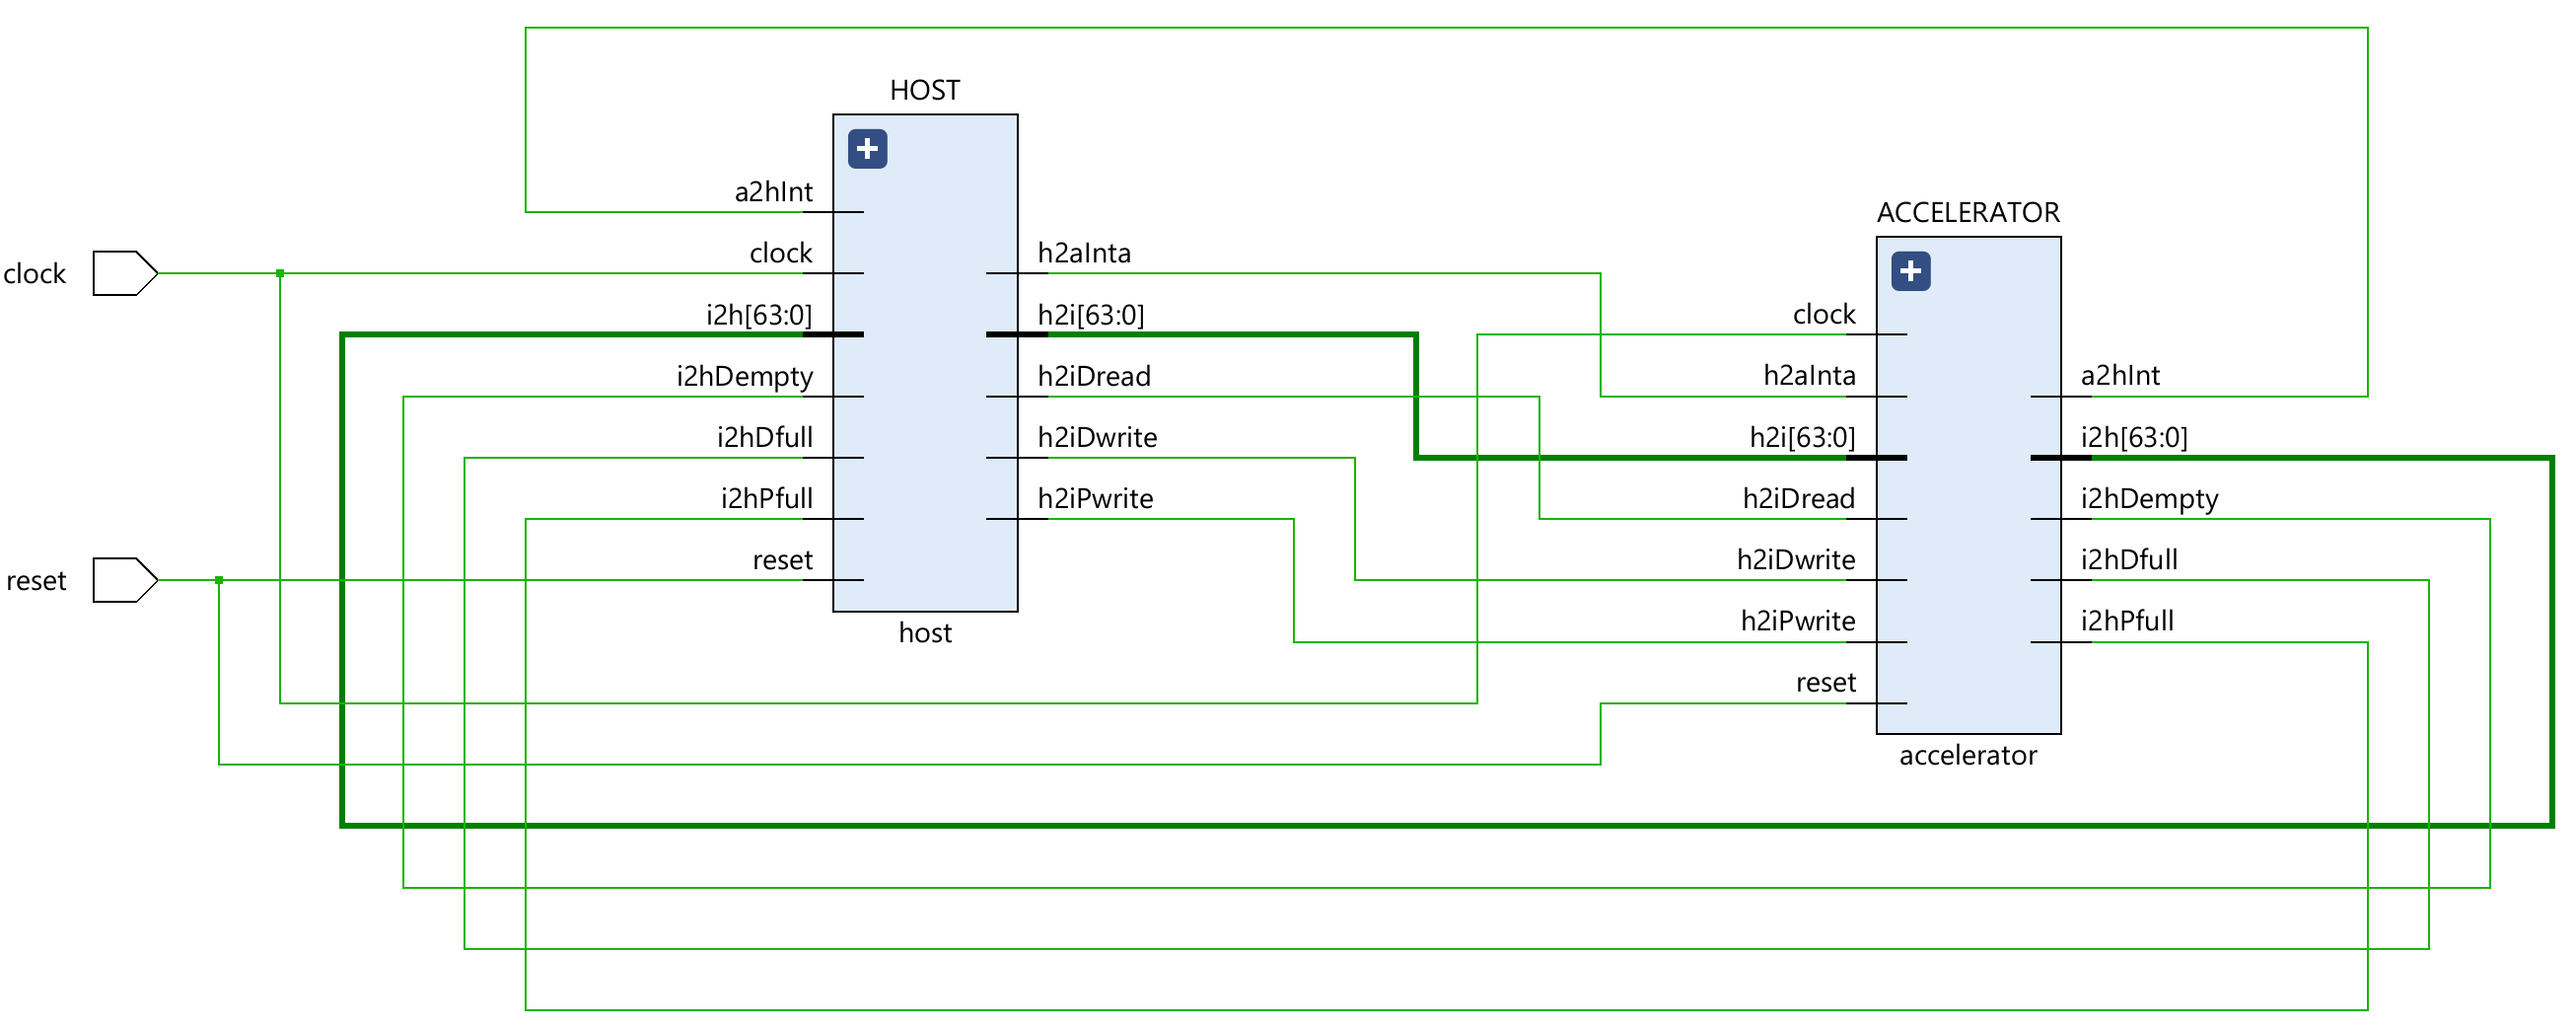
\includegraphics[width=\textwidth]{Images/hetSystTop.png} 
    \caption{The heterogeneous system.}
    \label{fig:hetSyst}
\end{figure}


%\placedrawing[H]{figures/20_1_heterogeneousSystem.lp}{Heterogeneous System ({\tt 1\_hetSys.sv}): HOST computer and many-cell ACCELERATOR interconnected through INTERFACES (three FIFOs: one for commands and programming and two for in and out of data).}{fighetSys}

\begin{description}
    \item[from HOST to ACCELERATOR:] program \& data 64-bit path and the synchronizing signals:
        \begin{description}
            \item[commands:] write programs, initialize programs and write data or transfer parameters; each transfer is done on 64-bit words per clock cycle
            \item[flags:] indicating that interfaces in ACCELERATOR are not ready to accept the current transfer of program or data
        \end{description}
    \item[from ACCELERATOR to HOST:] 64-bit data path and the synchronizing signals:
        \begin{description}
            \item[command:] sends to HOST data in 64-bit words
            \item[flag:] indicating that the interface ACCELERATOR in is not ready to send a 64-bit data word 
        \end{description}
    \item[synchronizing signals:] used to signal to  HOST the end of a computation generating an {\bf {\em interrupt}} answered by HOST. 
\end{description}

\includeverilogcode[caption={Heterogeneous system. File: 1\_hetSys.sv.  (SystemVerilog)}, 
                    label={lst:heterogeneousSystem}, 
                    firstline=1, 
                    firstnumber=1, 
                    lastline=68]
                    {\verilogSourceDir/A20_hetSys.sv}

%\placedrawing[H]{figures/20_2_accelerator.lp}{Accelerator ({\tt 2\_accelerator.sv}): the many-cell engine ARRAY and the sequencer CONTROLLER (a mono-core computer).}{figacc}

In the second level in the hierarchy, interesting from a parallel computing point of view is the accelerator whose top module is in Listing \ref{lst:accelerator}, while the entire design is on GitHub. The accelerator, see Figure \ref{fig:accelerator}, contains two modules:
\begin{itemize}
    \item {\tt interfaces}
    \item {\tt pRISC}: parallel RISC computational structure able to perform parallel computations
\end{itemize}

\includeverilogcode[caption={Accelerator. File: 1\_accelerator.sv.  (SystemVerilog)}, 
                    label={lst:accelerator}, 
                    firstline=1, 
                    firstnumber=1, 
                    lastline=68]
                    {\verilogSourceDir/A20_accelerator.sv}

\begin{figure}[H]
    \centering
    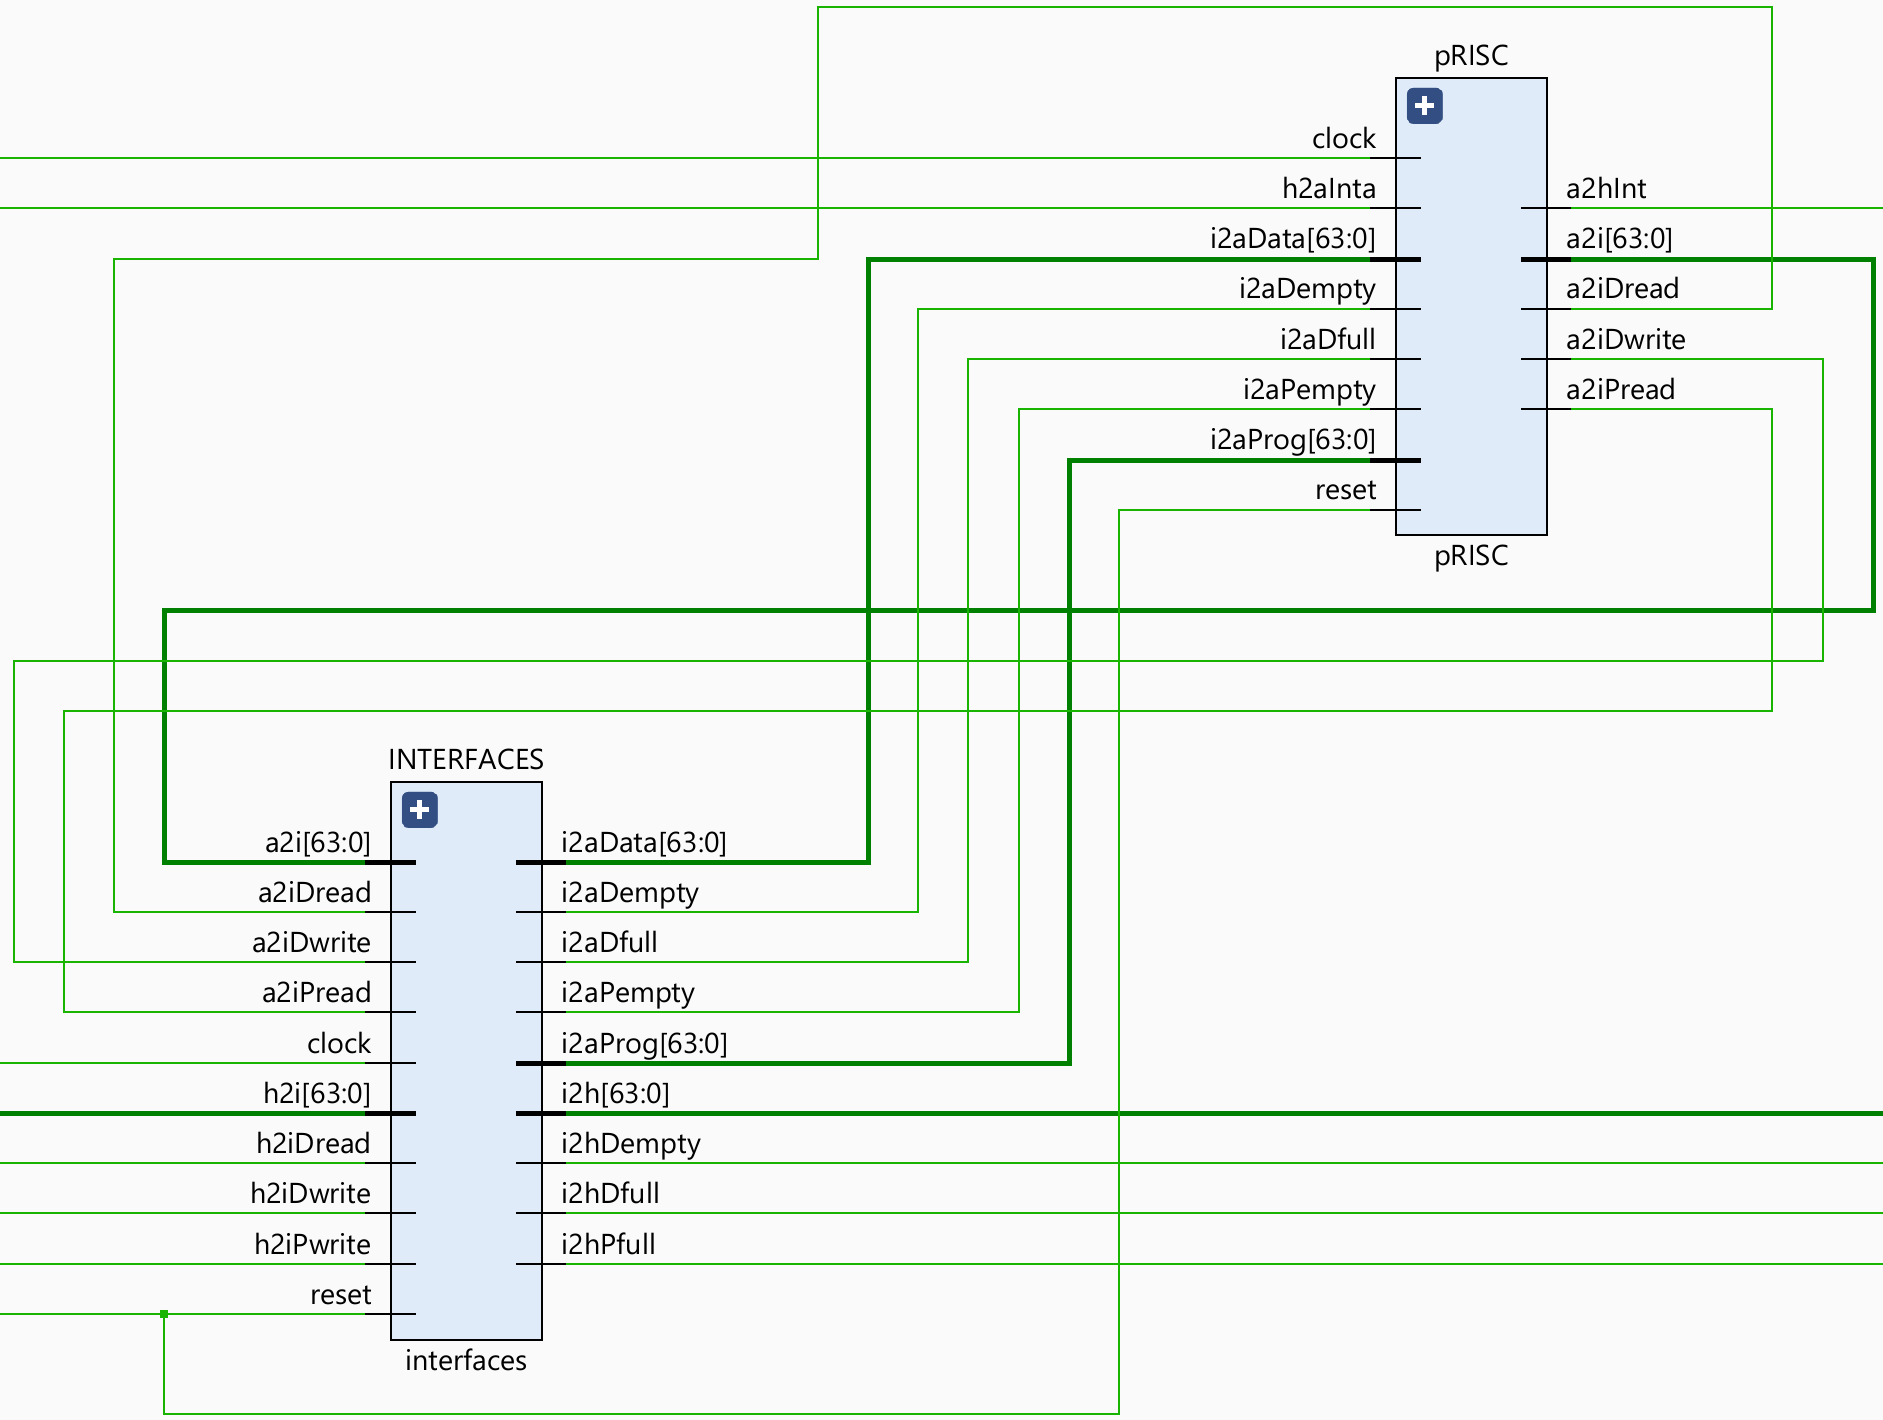
\includegraphics[width=\textwidth]{Images/hetAccelerator.png} 
    \caption{The accelerator.}
    \label{fig:accelerator}
\end{figure}

%\placedrawing[H]{figures/20_3_array.lp}{Array ({\tt 3\_array.sv}): the array of $p$ cells MAP loop connected with two $lor$-depth networks (REDUCE for reduce functions amd SCAN for scan functions).}{figarray}

The role of the interfaces (see Figure \ref{fig:hetInterfaces} and Listing \ref{lst:interfaces}) is to adapt the transfer rates, programs, commands and data, between the system host and the accelerator. The module contains three FIFO memories (see \ref{lb:fifo} in this book). One FIFO ensures the transfer of programs and commands from the host to the accelerator. The other two ensure the transfer of data from the host to the accelerator and vice versa.

\includeverilogcode[caption={Interfaces. File: 2\_interfaces.sv.  (SystemVerilog)}, 
                    label={lst:interfaces}, 
                    firstline=1, 
                    firstnumber=1, 
                    lastline=68]
                    {\verilogSourceDir/A20_interfaces.sv}

\begin{figure}[H]
    \centering
    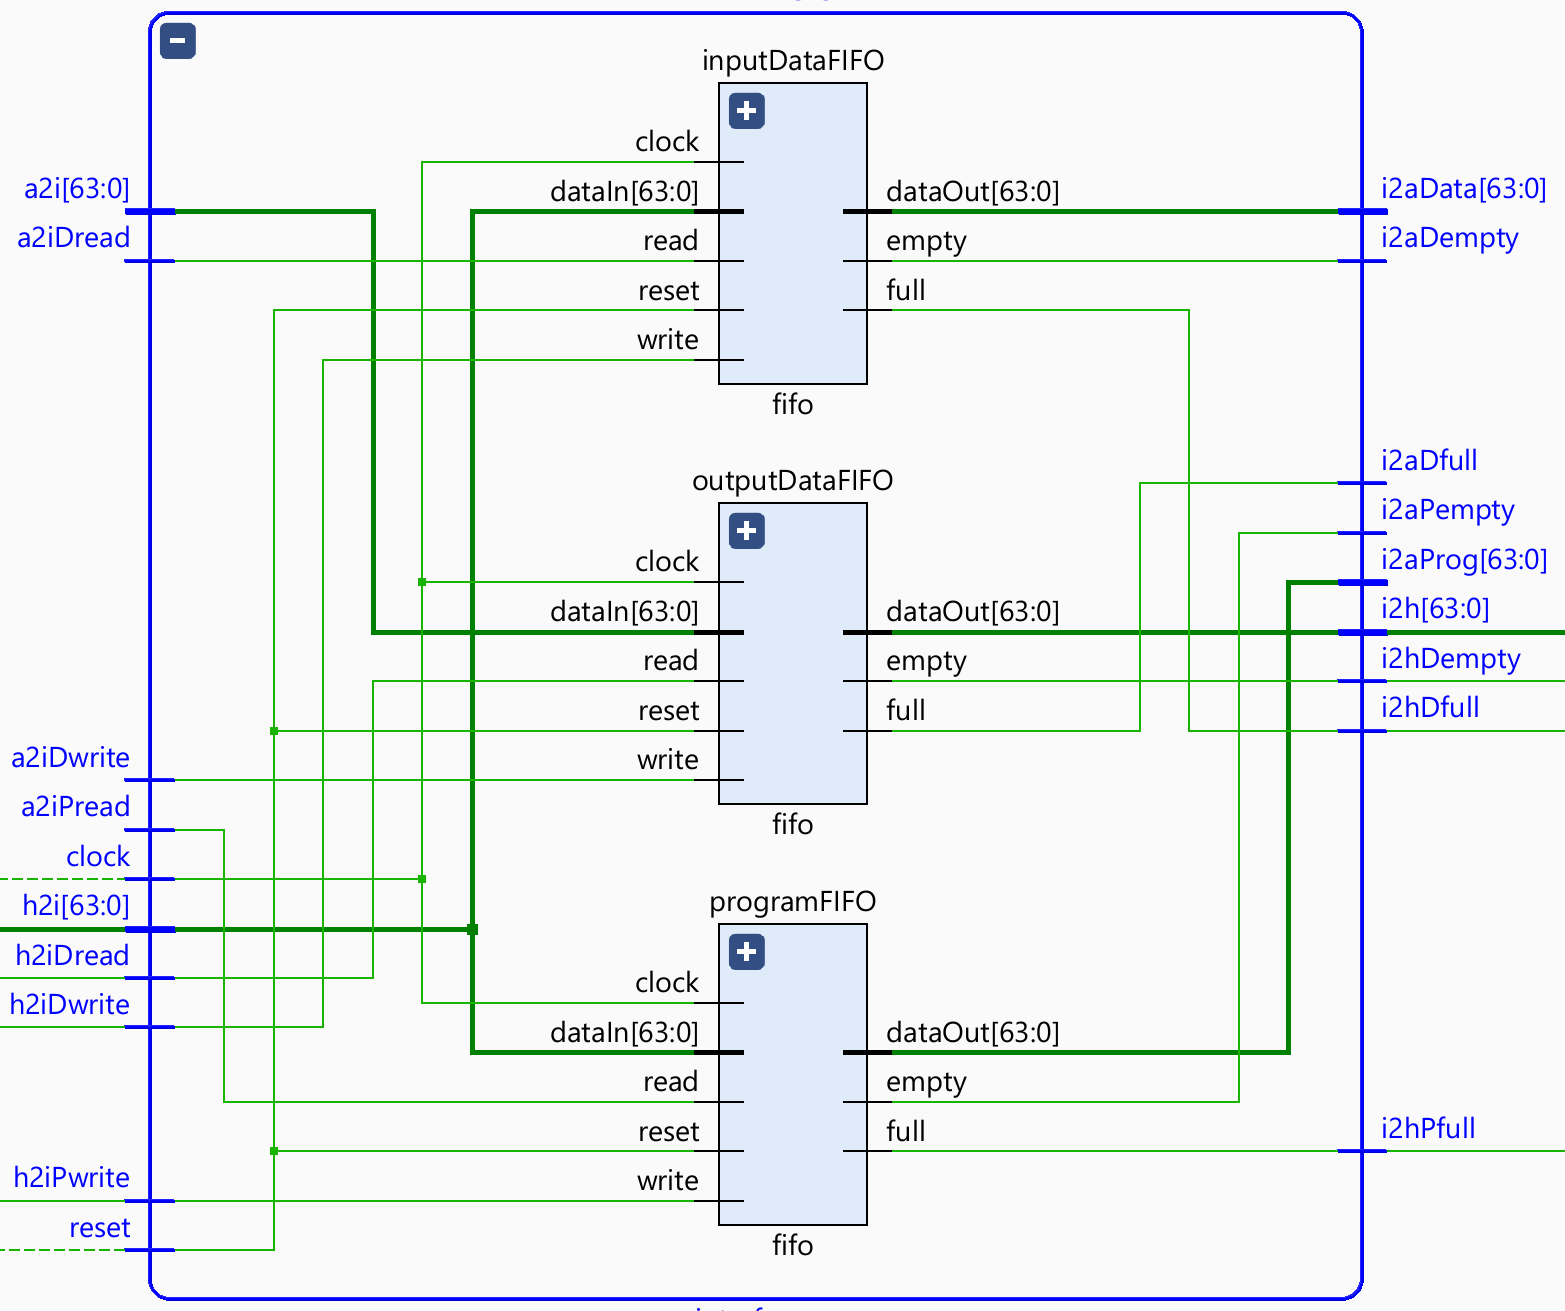
\includegraphics[width=\textwidth]{Images/hetInterfaces.png} 
    \caption{Interfaces.}
    \label{fig:hetInterfaces}
\end{figure}




pRISC\index{pRISC: parallel RISC architecture combining controller sequencer and linear cellular array}, which comes from {\em parallel RISC}\footnote{The name was proposed by Jim Peek\index{Peek, Jim: proposed pRISC parallel RISC name} \cite{Peek83} who as a master's student led the team of students who, at the initiative of professors David Patterson\index{Patterson, David (1947--): RISC and memory hierarchy pioneer} and Carlo Sequin\index{Sequin, Carlo: Berkeley RISC pioneer}, designed the first RISC processor in 1980 at Berkeley University (\url{https://www.computerhistory.org/revolution/digital-logic/12/286/1593}).} is the central component of the heterogeneous system we present. It is represented in Figure \ref{fig:pRISC} and codified in Listing \ref{lst:pRISC}, and consists of:
\begin{itemize}
    \item {\tt controller}: a RISC-based computer used as sequencer
    \item {\tt array}: a two-loop linear cellular array of execution units.
\end{itemize}

\begin{figure}[H]
    \centering
    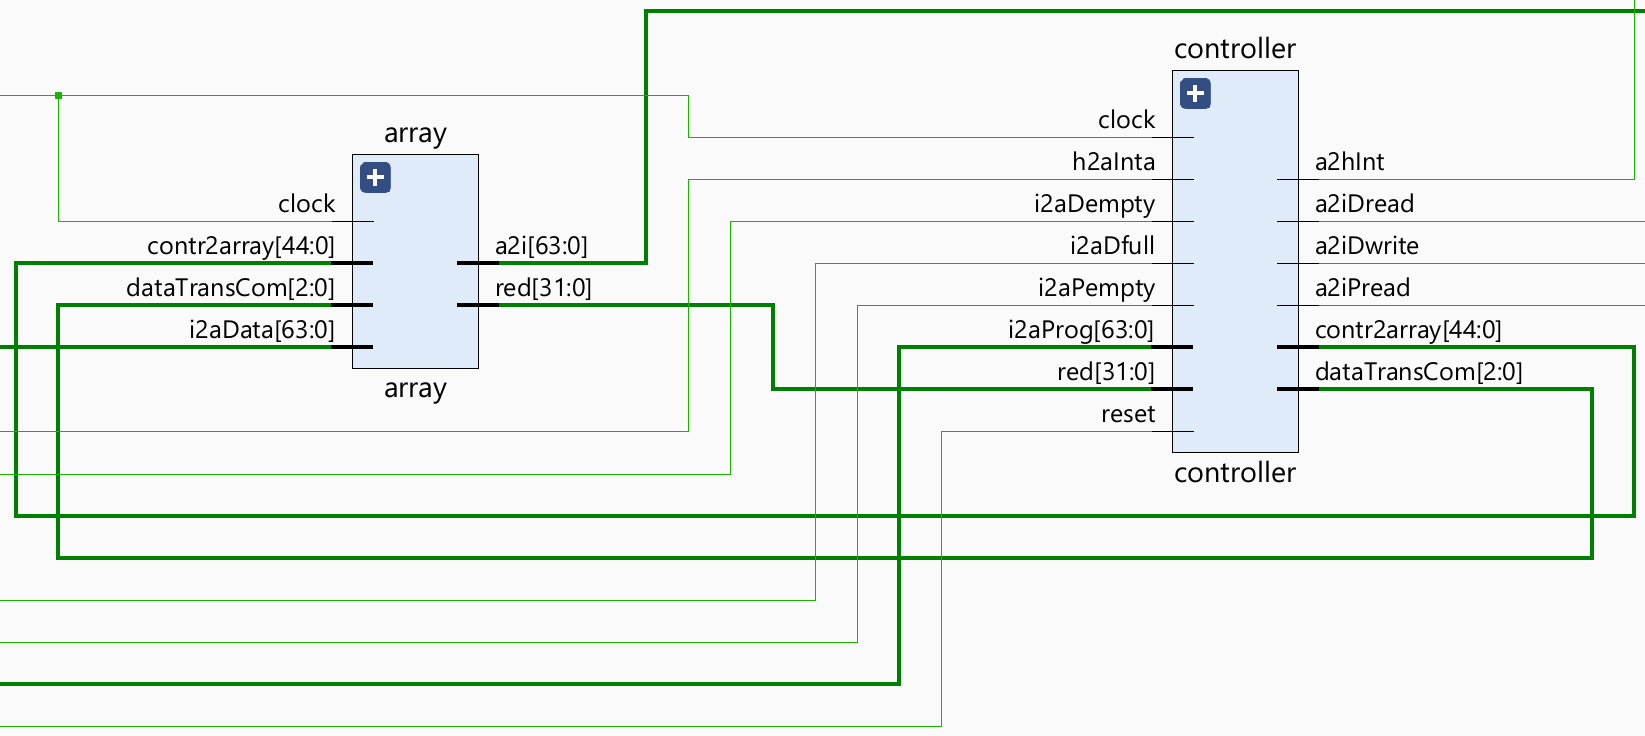
\includegraphics[width=\textwidth]{Images/pRISC.png} 
    \caption{Parallel RISC, pRISC.}
    \label{fig:pRISC}
\end{figure}

\includeverilogcode[caption={pRISC. File: 2\_pRISC.sv.  (SystemVerilog)}, 
                    label={lst:pRISC}, 
                    firstline=1, 
                    firstnumber=1, 
                    lastline=68]
                    {\verilogSourceDir/A20_pRISC.sv}

\begin{figure}[H]
    \centering
    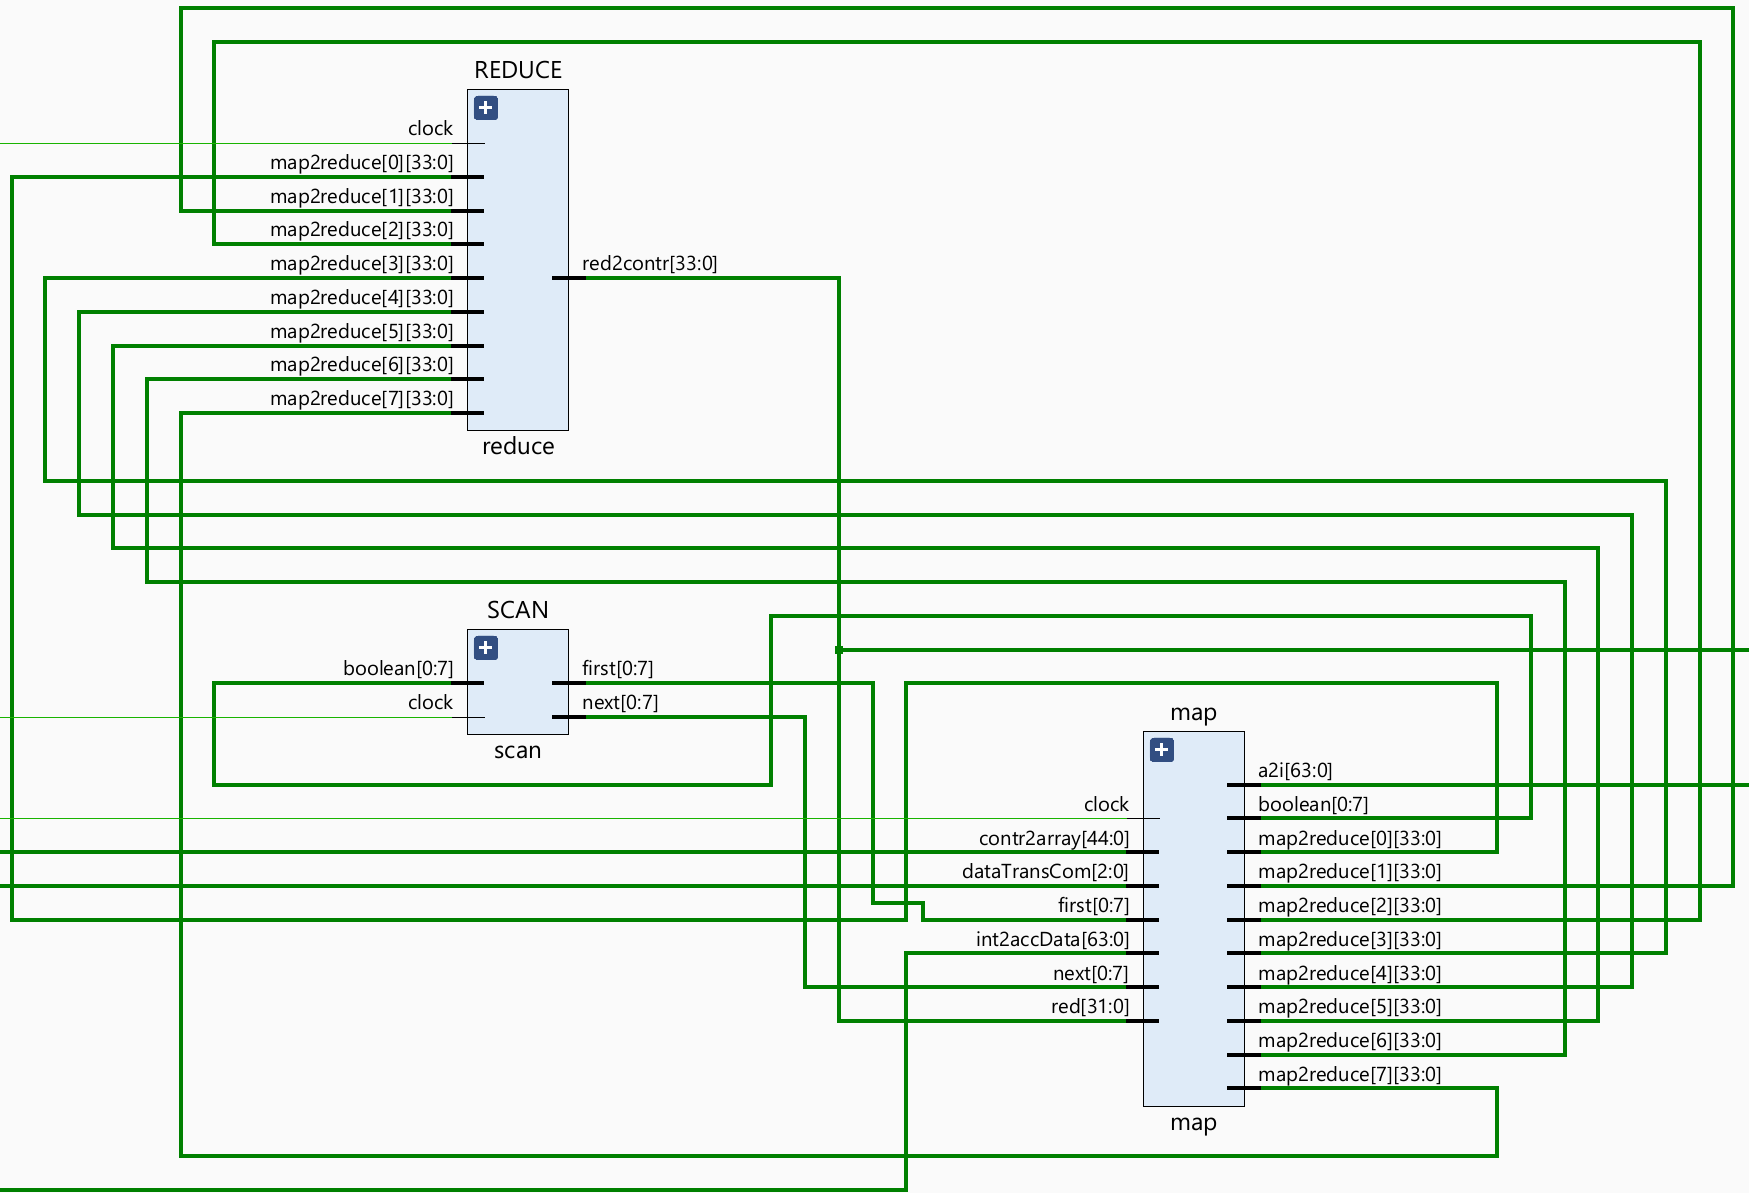
\includegraphics[width=\textwidth]{Images/hetArray.png} 
    \caption{Map array.}
    \label{fig:hetArray}
\end{figure}

While the controller is a well-established structure, the cellular area deserves explicit detail. It contains, see Figure \ref{fig:hetArray} and Listing \ref{lst:array} three functional components\index{Map-Scan-Reduce (MSR) network: parallel architecture network supporting map, scan, and reduce functions}:
\begin{itemize}
    \item the linear array of cells, {\tt map}\index{map array: linear array of parallel execution cells}, which includes the $log$-depth distribution network used to send in each clock cycle form controller to each cell an instruction with the associated value
    \item the first loop which reduces the vector, issued by the linear array of cells, to a scalar sent to the controller\index{reduce network: logarithmic network aggregating vector outputs to a scalar}
    \item the second loop which applies to the vector provided by the map section a scan function and sends back the resulting vector to the array\index{scan network: prefix computation network over cellular array vectors}.
\end{itemize}


\includeverilogcode[caption={Array. File: 3\_array.sv.  (SystemVerilog)}, 
                    label={lst:array}, 
                    firstline=1, 
                    firstnumber=1, 
                    lastline=68]
                    {\verilogSourceDir/A20_array.sv}

More details about the design of the heterogeneous system on GitHub.







\section{Micro-architectures}

The heterogeneous structure is defined by three micro-architectures, each describing the micro-operations performed at the lowest level in the system.

\subsection{Host micro-architecture}

The host's 32-bit micro-architecture is defined in Listing \ref{lst:hostDEFINES}. The associated instruction format is: 
\begin{verbatim}
    hInstr={opCode[5:0],dest[4:0],left[4:0],right[4:0],noUse[10:0]} | 
           {opCode[5:0],dest[4:0],left[4:0],val[15:0]}
\end{verbatim}
The internal state of the host (dimensioned with small memories to support fast simulation) is stored in:
\begin{description}
    \item[{\tt rf[0:31]}]: two-output port register file
    \item[{\tt cr}]: carry bit
    \item[{\tt pc[9:0]}]: program counter
    \item[{\tt hDmem[0:1023]}]: host data memory
    \item[{\tt hPmem[0:1023]}]: host program memory
\end{description}


\includeverilogcode[caption={Host micro-architecture.   (SystemVerilog)}, 
                    label={lst:hostDEFINES}, 
                    firstline=1, 
                    firstnumber=1, 
                    lastline=70]
                    {\verilogSourceDir/A20_hostDEFINES.vh}

\subsection{Accelerator micro-architecture}

The accelerator's micro-architecture is a Cartesian one, i.e., each micro-instruction belongs to a set which is a Cartesian product of two sets of micro-instructions. The two micro-architectures are: controller micro-architecture and map micro-architecture. 

\subsubsection{Controller micro-architecture}

The controller micro-architecture is defined in Listing \ref{lst:sequencerDEFINES}. It is an accumulator-based one, starting from the idea that for intense computation the complexity of the computing engine can and should be kept low.  The associated instruction format is: 
\begin{verbatim}
    sInstr={cOpcode[4:0], cMode[2:0], val[23:0]} | 
           {8'b11111_000, cOpcode[4:0], val[18:0]}
\end{verbatim}
The first instruction format refers to instructions using as left operand the accumulator, {\tt acc},  and the right operand, {\tt op}, the value, provided by {\tt value} from instruction, or the local memory content addressed by {\tt value} and, sometimes, a relative pointer {\tt addr}. The co-operand, {\tt coOp}, is the output of the Reduce network.

The internal state of the 32-bit word controller (dimensioned with small memories to support fast simulation) is stored in:
\begin{description}
    \item[{\tt cMem[0:1023]}]: one output port register file
    \item[{\tt acc}]: accumulator register
    \item[{\tt cAddr}]: relative address register
    \item[{\tt cr}]: carry bit
    \item[{\tt pc[9:0]}]: program counter
    \item[{\tt pMem[0:1023]}]: 64-bit word program memory
\end{description}

\includeverilogcode[caption={Controller micro-architecture.   (SystemVerilog)}, 
                    label={lst:sequencerDEFINES}, 
                    firstline=1, 
                    firstnumber=1, 
                    lastline=60]
                    {\verilogSourceDir/A20_sequencerDEFINES.vh}

\paragraph{Right operand select}
is specified by the 3-bit field,  {\tt cMode}  used to select the right operand  {\tt op} in SEQUENCER where:
\begin{verbatim}
            acc <= acc  cOpcode op
\end{verbatim}
The 5 modes of selecting the right operand are:
\begin{description}
    \item[imm] - the right operand, {\tt op}, is {\bf {\em imm}ediate}, given by the scalar provided in instruction:
        $${\tt op = val = \{\{8\{val[23]\}\}, value\}\}}$$
    \item[dir] - the right operand is read at the {\bf {\em dir}ect} address in data memory:
          $${\tt op = mem[value]}$$
    \item[rel] - right operand is read from the {\bf {\em rel}ative} to {\tt addr} address in data memory:
        $${\tt op = mem[addr + value]}$$
    \item[rei] - right operand is read from the {\bf {\em re}lative} to {\tt addr} address in data memory and the value of {\tt addr} is actualized ({\bf {\em i}ncremented}) to the current use:
        $${\tt op = mem; \;\; addr \Leftarrow addr + value}$$
    \item[cim] - right operand is the {\bf {\em c}o-operand} used {\bf {\em im}mediately}:
         $${\tt op = ReduceOut}$$
\end{description}

\subsubsection{Map micro-architecture}

The sequencer micro-architecture is defined in Listing \ref{lst:mapDEFINES}. It is an accumulator-based one, starting from the idea that for intense computation the complexity of the computing engine can and should be kept low. In addition, when we have a multicellular structure, it is good to keep the cells at a level of complexity and size as low as possible. The associated instruction format is:
\begin{verbatim}
    sInstr={mOpcode[4:0], mMode[2:0], val[23:0]} | 
           {8'b11111_000, mOpcode[4:0], val[18:0]}
\end{verbatim}
The first instruction format refers to instructions using as left operand the accumulator, {\tt acc},  and the right operand, {\tt op}, the value, provided by {\tt value} from instruction, or the local memory content addressed by {\tt value} and, sometimes, a relative pointer {\tt addr}. The co-operand, {\tt coOp}, is the accumulator of the sequencer, {\tt acc}.

The internal state of the Map array is stored in:
\begin{description}
    \item[distributed memory]: ${\bf M_{mp}}$  of form \\
    \[
   \begin{bmatrix}
    s[00] & s[01] & \dots  & s[0 p-1]\\
    s[10] & s[11] & \dots  & s[1 p-1]\\
    \vdots & \vdots & \ddots & \vdots\\
    s[m-1 0] & s[m-1 1] & \dots  & s[m-1 p-1]
    \end{bmatrix} = 
    \begin{bmatrix}
    V[0] \\
    V[1] \\
    \vdots \\
    V[m-1] 
    \end{bmatrix} =
    \begin{bmatrix}
    W[0] & W[1] & \dots  & W[p-1]
    \end{bmatrix}
    \]
    where: $V[i]$ are vector distributed along the Map array of cells, and $W[j]$ are "vertical" vectors stored in the local memories (register files) in each cell.
    \item[accumulator vector]:
     \[
    {\bf ACC_{p}} = \begin{bmatrix}
    acc[0] & acc[1] & \dots  & acc[p-1]
    \end{bmatrix}
    \]
    where: $acc[i]$ is the accumulator register in each cell
    \item[relative address vector]:
    \[
    {\bf ADDR_{p}} = \begin{bmatrix}
    addr[0] & addr[1] & \dots  & add[p-1]
    \end{bmatrix}
    \]
    where: $addr[i]$ is the relative addess used in each cell to address the local memory
    \item[Boolean vector]:
    \[
    {\bf B_{p}} = \begin{bmatrix}
    b[0] & b[1] & \dots  & b[p-1]
    \end{bmatrix}
    \]
    where: $b[i]$ is the bit indicating by value 1 the active cell 
    \item[carry vector]:
    \[
    {\bf CR_{p}} = \begin{bmatrix}
    cr[0] & cr[1] & \dots  & cr[p-1]
    \end{bmatrix}
    \]
    where: $cr[i]$ is the carry bit in each cell
    \item[index vector]:
    \[
    {\bf IX_{p}} = \begin{bmatrix}
    0 & ix_{1} & 1  & p-1
    \end{bmatrix}
    \]
    is used to identify the cell according to its position in the one-dimension array Map.
\end{description}

\includeverilogcode[caption={Map micro-architecture.   (SystemVerilog)}, 
                    label={lst:mapDEFINES}, 
                    firstline=1, 
                    firstnumber=1, 
                    lastline=60]
                    {\verilogSourceDir/A20_mapDEFINES.vh}

\paragraph{Right operand select} is specified by the 3-bit field,  {\tt mMode}  used to select the right operand  {\tt op} in each cell from MAP where:
\begin{verbatim}
            acc[i] <= acc[i]  mOpcode op
\end{verbatim}
The 8 modes of selecting the right operand are:
\begin{description}
    \item[imm] - right operand, {\tt op}, is {\bf {\em imm}ediate}, given by the scalar provided in instruction:
        $${\tt op[i] = val = \{\{8\{val[23]\}\}, val\}}$$
    \item[dir] - right operand is read from the {\bf {\em dir}ect} address in data memory:
         $${\tt op[i] = vectMmem[val]}$$
    \item[rel] - right operand is read from the {\bf {\em rel}ative} to {\tt addr} address in data memory:
         $${\tt op[i] = mem[addr[i] + val]}$$
    \item[rei] - right operand is read from the {\bf {\em re}lative} to {\tt addr} address in data memory and the value of {\tt addr} is actualized ({\bf {\em i}ncremented}) to the current use:
         $${\tt op[i]    = mem[addr[i] + val]; \;\; addr[i] <= addr[i] + val}$$
    \item[cim] - right operand is the {\bf {\em c}o-operand} used {\bf {\em im}mediately}, i.e., {\tt acc}:
        $${\tt op[i] = acc}$$
    \item[cdr] - operation is performed similar with {\tt dir} mode but the memory location is selected by the {\bf {\em c}o-operand} used {\bf {\em d}i{\em r}ect} as address
        $${\tt op[i] = mem[acc]}$$
     \item[crl] - similar with {\tt rel}, but the {\tt addr} value is incremented with the {\bf {\em c}o-operand} used as {\bf {\em r}e{\em l}ative} address
       $${\tt op[i] = mem[addr[i] + acc]}$$
     \item[cri] - similar with {\tt rei}, but the {\tt addr} value is incremented with the {\bf {\em c}o-operand} used as {\bf {\em r}elative} address whose value is also {\bf {\em i}ncrementad}
        $${\tt op[i] = mem[addr[i] + acc]; \;\; addr[i] <= addr[i] + acc}$$
\end{description}

\subsection{Putting all together}

The previously defined three micro-architecture are assembled in a unique file, {\tt 0\_DEFINES.vh}.

\includeverilogcode[caption={Micro-architectures. File: {\tt 0\_DEFINES.vh}.   (SystemVerilog)}, 
                    label={lst:DEFINES}, 
                    firstline=1, 
                    firstnumber=1, 
                    lastline=60]
                    {\verilogSourceDir/A20_DEFINES.vh}


\section{Heterogeneous architecture}

The general architecture of the hRISC heterogeneous system consists of the toyRISC architecture and the dual pRISC architecture. 

\subsection{Host architecture}

The host architecture will be described through the host's instruction set architecture (hISA) and a version 0.1 function library architecture (FLA 0.1) that we propose.

\subsubsection{Instruction set}



%\begin{table}[H]
{\small
{\centering
\begin{longtable}{|l|l|l|}
\caption{Host's Instruction Set Architecture.}
\label{tab:host_isa} \\
\hline
\textbf{OpCode} & \textbf{Commentaries} & \textbf{Assembly} \\
\hline
\endfirsthead
\hline
\textbf{OpCode} & \textbf{Commentaries} & \textbf{Assembly} \\
\hline
\endhead
\hline
\endfoot
\hline
\endlastfoot
\multicolumn{3}{|c|}{\textbf{CONTROL OPERATIONS}} \\
\hline
nop    & no operation: \texttt{pc <= pc+1}                            & hNOP          \\ \hline
hjmp   & relative jump: \texttt{pc <= pc+val}                         & hJMP(lb)      \\ \hline
hjmpz  & conditioned jump: \texttt{pc <= (rf[left]==0) ? pc+val : pc+1} & hJMPZ(l, lb)  \\ \hline
hjmpnz & conditioned jump: \texttt{pc <= (rf[left]==0) ? pc+1 : pc+val} & hJMPNZ(l, lb) \\ \hline
hajmp  & absolute jump: \texttt{pc <= pc + val}                       & hAJMP(val)    \\ \hline
hhalt  & halt: \texttt{pc <= pc}                                      & hHALT         \\ \hline
hpsend & send to Map a auto-delimited program                         & hPSEND(d, l)  \\ \hline
hdget  & get from Map a stream of data                                & hDGET(d, l, r) \\ \hline
hdsend & send to Map a stream of data                                 & hDSEND(d, l, r) \\ \hline
hintwait & interrupt wait                                             & hINTWAIT      \\ \hline
hsttcc & start host's cycle counter                                   & hSTARTCC      \\ \hline
hstpcc & stop host's cycle counter                                    & hSTOPCC       \\ \hline
\multicolumn{3}{|c|}{\textbf{FUNCTIONAL OPERATIONS}} \\
\hline
hadd   & \texttt{\{cr, rf[dest]\} <= rf[left] + rf[right]}            & hADD(d, l, r) \\ \hline
haddcr & \texttt{\{cr, rf[dest]\} <= rf[left] + rf[right] + cr}       & hADDCR(d, l, r) \\ \hline
hsub   & \texttt{\{cr, rf[dest]\} <= rf[left] - rf[right]}            & hSUB(d, l, r) \\ \hline
hsubcr & \texttt{\{cr, rf[dest]\} <= rf[left] - rf[right] - cr}       & hSUBCR(d, l, r) \\ \hline
hmult  & \texttt{\{cr, rf[dest]\} <= \{cr, rf[left] * rf[right]\}}    & hMULT(d, l, r) \\ \hline
hbwand & \texttt{\{cr, rf[dest]\} <= \{cr, rf[left] \& rf[right]\}}   & hAND(d, l, r) \\ \hline
hbwor  & \texttt{\{cr, rf[dest]\} <= \{cr, rf[left] | rf[right]\}}    & hOR(d, l, r)  \\ \hline
hbwxor & \texttt{\{cr, rf[dest]\} <= \{cr, rf[left] $\wedge$ rf[right]\}} & hXOR(d, l, r) \\ \hline
haddv  & \texttt{\{cr, rf[dest]\} <= rf[left] + val}                  & hADDV(d, l, val) \\ \hline
haddcrv & \texttt{\{cr, rf[dest]\} <= rf[left] + val + cr}            & hADDCRV(d, l, val) \\ \hline
hsubv  & \texttt{\{cr, rf[dest]\} <= rf[left] - val}                  & hSUBV(d, l, val) \\ \hline
hsubcrv & \texttt{\{cr, rf[dest]\} <= rf[left] - val - cr}            & hSUBCRV(d, l, val) \\ \hline
hmultv & \texttt{\{cr, rf[dest]\} <= \{cr, rf[left] * val\}}          & hMULTV(d, l, val) \\ \hline
hbwandv & \texttt{\{cr, rf[dest]\} <= \{cr, rf[left] \& val\}}        & hANDV(d, l, val) \\ \hline
hbworv & \texttt{\{cr, rf[dest]\} <= \{cr, rf[left] | val\}}          & hORV(d, l, val) \\ \hline
hbwxorv & \texttt{\{cr, rf[dest]\} <= \{cr, rf[left] $\wedge$ val\}}  & hXORV(d, l, val) \\ \hline
\multicolumn{3}{|c|}{\textbf{DATA TRANSFER INSTRUCTIONS}} \\
\hline
hvalue  & \texttt{\{cr, rf[dest]\} <= \{cr, \{16\{val[15]\}\}, val\}} & hVALUE(d, val) \\ \hline
hinsval & \texttt{\{cr, rf[dest]\} <= \{cr, \{rf[left][15:0], val\}\}} & hINSVAL(d, val) \\ \hline
hload   & \texttt{\{cr, rf[dest]\} <= \{cr, hDmem[rf[left]]\}}        & hLOAD(d, l)    \\ \hline
hstore  & \texttt{hDmem[rf[left]] <= rf[right]}                       & hSTORE(l, r)   \\ \hline
\end{longtable}
}
}
%\end{table}





\subsubsection{Low-level library of functions (FLA 0.1)}

An assembly program written for the host computer uses the hISA, and a first version of a  library of functions, LFA 0.1 (see Table \ref{tab:lfa01}), where each function is implemented by a program executed by the accelerator. Thus, the library used by host is a hardware implemented library unlike the usual software-designed libraries.

%\begin{table}[H]
{\small
{\centering
\begin{longtable}{|l|l|}
\caption{Host's Function Library Architecture (FLA) defined in file: {\tt 00\_theKernel.sv}.}
\label{tab:lfa01} \\
\hline
\textbf{Assembly} & \textbf{Commentaries} \\
\hline
\endfirsthead
\hline
\textbf{Assembly} & \textbf{Commentaries} \\
\hline
\endhead
\hline
\endfoot
\hline
\endlastfoot
hSTART           & Start controller's cycle counter \\ \hline
hSTOP            & Stop controller's cycle counter \\ \hline
hINTRQ           & Interrupt request \\ \hline
hVGENX(addr)     & \texttt{V(addr) <= IX} \\ \hline
hVGENN(addr,val) & \texttt{V(addr) <= [val val ... val]} \\ \hline
hSQGENX          & Generate square matrix \texttt{[V[0]=IX V[1]=IX+1 ... V[p-1]=IX+p-1]} \\ \hline
hSQGENN(val)     & Generate square matrix with \texttt{V[i]= [val val ... val]}, for \(i = 0, ..., p-1\) \\ \hline
hMAIN(d,val)      & Generate diagonal matrix starting with \texttt{V[s]} with value {|tt val}  \\ \hline
hPRANDOM(d)      & Generate pseudo-random square matrix starting with \texttt{V[d]} \\ \hline
hMSEND(addr,size)& Send square matrix of \texttt{size} starting from \texttt{V[addr]} \\ \hline
hMGET(addr,size) & Get square matrix of \texttt{size} and load from \texttt{V[addr]} \\ \hline
hSQMADD(d,l,r)   & \texttt{Add square matrices: M[d] <= M[l] + M[r]} \\ \hline
hSQMVMULT(d,l,r) & \texttt{Multiply square matrices with vector: V[d] <= M[l] * V[r]} \\ \hline
hSQMMULT(d,l,r)  & \texttt{Square matrices multiply: M[d] <= M[l] * M[r]} \\ \hline
hSQMMAC(d,l,r)   & \texttt{Square matrices multiply and add: M[d] <= M[d] + (M[l] * M[r])} \\ \hline
hTRANS(d,l)   & \texttt{Transpose square matrix: M[d] <= trans(M[l])} \\ \hline
\end{longtable}
}
}
%\end{table}
In Table \ref{tab:lfa01}, {\tt M[v]} represents a $p \times p$ square matrix  with the first vector {\tt V[a]} and the last vector {\tt V[a+p-1]}.

\subsection{Accelerator's dual architecture}

\subsubsection{Controller's architecture}

Each assembly-level instruction is made by concatenating the operation micro-code (indicated on the first column of the following tables) with the micro-code that selects the operation mode (indicated on the first line in the following table).


%\begin{table}[H]
{\small
{\centering
\begin{longtable}{|l||l|l|l|l|l|}
\caption{Instructions with operands from the controller's Instruction Set Architecture.}
\label{tab:controller_isa} \\
\hline
\textbf{cOpcode $\setminus$ cMode} & \textbf{imm} & \textbf{dir} & \textbf{rel} & \textbf{rei} & \textbf{cim} \\
\hline
\endfirsthead
\hline
\textbf{cOpcode $\setminus$ cMode} & \textbf{imm} & \textbf{dir} & \textbf{rel} & \textbf{rei} & \textbf{cim} \\
\hline
\endhead
\hline
\endfoot
\hline
\endlastfoot
cadd      & cVADD(s)    & cADD(s)    & cRADD(s)    & cRIADD(s)    & CADD       \\ \hline
caddc     & cVADDC(s)   & cADDC(s)   & cRADDC(s)   & cRIADDC(s)   & CADDC      \\ \hline
csub      & cVSUB(s)    & cSUB(s)    & cRSUB(s)    & cRISUB(s)    & CSUB       \\ \hline
crsub     & cVRSUB(s)   & cRSUB(s)   & cRRSUB(s)   & cRIRSUB(s)   & CRSUB      \\ \hline
csubc     & cVSUBC(s)   & cSUBC(s)   & cRSUBC(s)   & cRISUBC(s)   & CSUBC      \\ \hline
crsubc    & cVRSUBC(s)  & cRSUBC(s)  & cRRSUBC(s)  & cRIRSUBC(s)  & CRSUBC     \\ \hline
cmult     & cVMULT(s)   & cMULT(s)   & cRMULT(s)   & cRIMULT(s)   & CMULT      \\ \hline
cbwand    & cVAND(s)    & cAND(s)    & cRAND(s)    & cRIAND(s)    & CAND       \\ \hline
cbwor     & cVOR(s)     & cOR(s)     & cROR(s)     & cRIOR(s)     & COR        \\ \hline
cbwxor    & cVXOR(s)    & cXOR(s)    & cRXOR(s)    & cRIXOR(s)    & CXOR       \\ \hline
cload     & cVLOAD(s)   & cLOAD(s)   & cRLOAD(s)   & cRILOAD(s)   & CLOAD      \\ \hline
cstore    &             & cSTORE(s)  & cRSTORE(s)  & cRISTORE(s)  & CCSTORE    \\ \hline
\end{longtable}
}}
%\end{table}




%\begin{table}[H]
{\small
{\centering
\begin{longtable}{|l|l|l|}
\caption{Sequencer's Instruction Set Architecture with no operand.}
\label{tab:sequencer_isa} \\
\hline
\textbf{\{cOpcode, value[2:0]\}} & \textbf{Commentaries}                         & \textbf{Assembly}    \\
\hline
\endfirsthead
\hline
\textbf{\{cOpcode, value[2:0]\}} & \textbf{Commentaries}                         & \textbf{Assembly}    \\
\hline
\endhead
\hline
\endfoot
\hline
\endlastfoot
\{cshift,4\}   & Shift right one bit position                  & cSHR         \\ \hline
\{cshift,5\}   & Shift right arithmetic one bit position       & cASHR        \\ \hline
\{cshift,6\}   & Shift right one bit position with carry       & cSHRC        \\ \hline
\{cshift,1\}   & Shift left one bit position                   & cSHL         \\ \hline
\{cshift,2\}   & Shift left one bit position with carry        & cSHLC        \\ \hline
\{cshift,7\}   & Rotate right one bit position                 & cROTR        \\ \hline
\{cshift,3\}   & Rotate left one bit position                  & cROTL        \\ \hline
\{gshift,0\}   & 1-position global right shift                 & cGRSHIFT     \\ \hline
\{gshift,1\}   & 1-position global left shift                  & cGLSHIFT     \\ \hline
\{gshift,5\}   & Reduction output insert right                 & cRREDINS     \\ \hline
\{gshift,4\}   & Reduction output insert left                  & cLREDINS     \\ \hline
\{gshift,2\}   & 1-position global right rotate                & cGRROTATE    \\ \hline
\{gshift,3\}   & 1-position global left rotate                 & cGLROTATE    \\ \hline
nop            & No operation                                  & cNOP         \\ \hline
jmp            & Relative jump to label \(s\)                 & cJMP(s)      \\ \hline
ajmp           & Absolute jump to label \(s\)                 & cAJMP(s)     \\ \hline
brz            & Jump to label \(s\) if \texttt{acc=0}         & cBRZ(s)      \\ \hline
brnz           & Jump to label \(s\) if \texttt{acc!=0}        & cBRNZ(s)     \\ \hline
brzdec         & Jump to label \(s\) if \texttt{acc=0}; \texttt{acc<=acc-1} & cBRZDEC(s)   \\ \hline
brnzdec        & Jump to label \(s\) if \texttt{acc!=0}; \texttt{acc<=acc-1} & cBRNZDEC(s)  \\ \hline
halt           & \texttt{pc <= pc}                            & cHALT        \\ \hline
cinsval        & \texttt{acc <= \{(acc << 8), value[7:0]\}}    & cINSVAL      \\ \hline
crela          & \texttt{addr <= acc}                         & cADDRLD      \\ \hline
start          & Start cycle counter                          & cSTART       \\ \hline
stop           & Stop cycle counter                           & cSTOP        \\ \hline
\end{longtable}
}}
%\end{table}



\subsubsection{Map's architecture}

Each assembly-level instruction is made by concatenating the operation micro-code (indicated on the first column of the following tables) with the micro-code that selects the operation mode (indicated on the first line in the following table).

%\begin{table}[H]
{\scriptsize
{\centering
\begin{longtable}{|p{7mm}|p{16.5mm}|p{12mm}|l|l|l|l|l|l|}
\caption{Instructions with operands from the Instruction Set Architecture.}
\label{table:isa_instructions} \\
\hline
 & \textbf{imm} & \textbf{dir} & \textbf{rel} & \textbf{rei} & \textbf{cim} & \textbf{cdr} & \textbf{crl} & \textbf{cri} \\
\hline
\endfirsthead
\hline
 & \textbf{imm} & \textbf{dir} & \textbf{rel} & \textbf{rei} & \textbf{cim} & \textbf{cdr} & \textbf{crl} & \textbf{cri} \\
\hline
\endhead
\hline
\endfoot
\hline
\endlastfoot
add       & VADD(s)    & ADD(s)    & RADD(s)    & RIADD(s)    & CADD    & CAADD    & CRADD    & CRIADD    \\ \hline
addc      & VADDC(s)   & ADDC(s)   & RADDC(s)   & RIADDC(s)   & CADDC   & CAADDC   & CRADDC   & CRIADDC   \\ \hline
sub       & VSUB(s)    & SUB(s)    & RSUB(s)    & RISUB(s)    & CSUB    & CASUB    & CRSUB    & CRISUB    \\ \hline
rsub      & VRSUB(s)   & RSUB(s)   & RRSUB(s)   & RIRSUB(s)   & CRSUB   & CARSUB   & CRRSUB   & CIRRSUB   \\ \hline
subc      & VSUBC(s)   & SUBC(s)   & RSUBC(s)   & RISUBC(s)   & CSUBC   & CASUBC   & CRSUBC   & CRISUBC   \\ \hline
rsubc     & VRSUBC(s)  & RSUBC(s)  & RRSUBC(s)  & RIRSUBC(s)  & CRSUBC  & CARSUBC  & CRRSUBC  & CRIRSUBC  \\ \hline
mult      & VMULT(s)   & MULT(s)   & RMULT(s)   & RIMULT(s)   & CMULT   & CAMULT   & CRMULT   & CRIMULT   \\ \hline
bwand     & VAND(s)    & AND(s)    & RAND(s)    & RIAND(s)    & CAND    & CAAND    & CRAND    & CRIAND    \\ \hline
bwor      & VOR(s)     & OR(s)     & ROR(s)     & RIOR(s)     & COR     & CAOR     & CROR     & CRIOR     \\ \hline
bwxor     & VXOR(s)    & XOR(s)    & RXOR(s)    & RIXOR(s)    & CXOR    & CAXOR    & CRXOR    & CRIXOR    \\ \hline
load      & VLOAD(s)   & LOAD(s)   & RLOAD(s)   & RILOAD(s)   & CLOAD   & CALOAD   & CRLOAD   & CRILOAD   \\ \hline
store     &            & STORE(s)  & RSTORE(s)  & RISTORE(s)  & CSTORE  & CASTORE  & CRSTORE  & CRISTORE  \\ \hline
getio     &            & GETIO(s)  &            & RIGETIO(s)  &         &          &          &           \\ \hline
sendio    &            & SENDIO(s) &            & RISENDIO(s) &         &          &          &           \\ \hline
search    & VSEARCH(s) &           &            &             & SEARCH  &          &          &           \\ \hline
csearch   & VCSEARCH(s)&           &            &             & CSEARCH &          &          &           \\ \hline
insert    & VINSERT(s) &           &            &             & INSERT  &          &          &           \\ \hline
\end{longtable}
}}
%\end{table}


%\begin{table}[H]
{\small
{\centering
\begin{longtable}{|l|l|l|}
\caption{Map's Instruction Set Architecture with no operand.}
\label{tab:map_isa} \\
\hline
\textbf{\{cOpcode, value[2:0]\}} & \textbf{Commentaries} & \textbf{Assembly} \\
\hline
\endfirsthead
\hline
\textbf{\{cOpcode, value[2:0]\}} & \textbf{Commentaries} & \textbf{Assembly} \\
\hline
\endhead
\hline
\endfoot
\hline
\endlastfoot
\{shift,4\}   & Shift right one bit position                     & SHR            \\ \hline
\{shift,5\}   & Shift right arithmetic one bit position          & ASHR           \\ \hline
\{shift,6\}   & Shift right one bit position with carry          & SHRC           \\ \hline
\{shift,1\}   & Shift left one bit position                      & SHL            \\ \hline
\{shift,2\}   & Shift left one bit position with carry           & SHLC           \\ \hline
\{shift,7\}   & Rotate right one bit position                    & ROTR           \\ \hline
\{shift,3\}   & Rotate left one bit position                     & ROTL           \\ \hline
ixload        & \texttt{acc[i] <= i}                             & IXLOAD         \\ \hline
getsr         & \texttt{acc[i] <= serialReg[i]}                  & GETSR          \\ \hline
sendsr        & \texttt{serialReg[i] <= acc[i]}                  & SENDSR         \\ \hline
\{where,0\}   & \texttt{b[i] <= (b[i] \& acc[i]=0) ? 1 : 0}       & WHEREZERO      \\ \hline
\{where,1\}   & \texttt{b[i] <= (b[i] \& carry[i]) ? 1 : 0}       & WHERECARRY     \\ \hline
\{where,2\}   & \texttt{b[i] <= (b[i] \& acc[i][31]=1) ? 1 : 0}   & WHERENEGATIVE  \\ \hline
\{where,3\}   & \texttt{b[i] <= i=0 ? 0 : (b[i-1] ? 1 : 0)}       & WHEREPREVACT   \\ \hline
\{where,4\}   & \texttt{b[i] <= (b[i] \& first ? 1 : 0)}          & WHEREFIRST     \\ \hline
\{where,5\}   & \texttt{b[i] <= (b[i] \& next ? 1 : 0)}           & WHERENEXT      \\ \hline
\{where,6\}   & \texttt{b[i] <= (b[i] \& !(first | next)) ? 1 : 0} & WHEREPREV      \\ \hline
\{where,8\}   & \texttt{b[i] <= (b[i] \& !(acc[i]=0)) ? 1 : 0}    & WHERENZERO     \\ \hline
\{where,9\}   & \texttt{b[i] <= (b[i] \& !carry[i]) ? 1 : 0}      & WHERENCARRY    \\ \hline
\{where,10\}  & \texttt{b[i] <= (b[i] \& !(acc[i][31]=1)) ? 1 : 0} & WHERENNEGATIVE \\ \hline
\{where,11\}  & \texttt{b[i] <= i=0 ? 1 : (b[i-1] ? 0 : 1)}       & WHERENPREVACT  \\ \hline
\{where,12\}  & \texttt{b[i] <= (b[i] \& !first) ? 1 : 0}         & WHERENFIRST    \\ \hline
\{where,13\}  & \texttt{b[i] <= (b[i] \& !next) ? 1 : 0}          & WHERENNEXT     \\ \hline
\{where,14\}  & \texttt{b[i] <= (b[i] \& (first | next)) ? 1 : 0} & WHERENPREV     \\ \hline
elsew         & Reapply the last \texttt{where} with the negated condition & ELSEWHERE     \\ \hline
back          & Redo \texttt{b[i]} affected by the most recently active where & ENDWHERE     \\ \hline
selsh         & \texttt{b[i] <= i=0 ? 0 : b[i-1]}                 & SELSHIFT       \\ \hline
allact        & \texttt{b[i] <= 1}                                & ACTIVATE       \\ \hline
\{setred,0\}  & Set the reduction function on addition            & REDADD         \\ \hline
\{setred,3\}  & Set the reduction function on minimum             & REDMIN         \\ \hline
\{setred,2\}  & Set the reduction function on maximum             & REDMAX         \\ \hline
\{setred,1\}  & Set the reduction function on logical OR          & REDOR          \\ \hline
delete        &                                                  & DELETE         \\ \hline
cinsval       & \texttt{acc[i] <= \{(acc[i] << 8), value[7:0]\}}  & INSVAL         \\ \hline
crela         & \texttt{addr[i] <= acc[i]}                       & ADDRLD         \\ \hline
\end{longtable}
}}
%\end{table}



\section{Programming heterogeneous system}

The simulation program ensures the initial loading of the HOST memory with the program it runs as well as with the program that the HOST loads into the ACCELERATOR during the system initialization process. If applicable, the HOST data memory is also initialized by the simulation program using a text file.

The heterogeneous system runs two programs simultaneously. They are assembled independently and are launched together. The program on the host is the one that loads the program into the accelerator. In listing \ref{lst:hProgram}:
\begin{itemize}
    \item line 1 loads in {\tt rf[0]} the initial address in the host's data memory from where the program must be sent to the accelerator; it is 0
    \item line 2 sends the program stored in data memory at the address from {\tt rf[0]} to the address 0 in the program memory of the accelerator
\end{itemize}

\includeverilogcode[caption={The framework in which the host program must be included. File: 0\_hProgram.sv  (SystemVerilog)}, 
                    label={lst:hProgram}, 
                    firstline=1, 
                    firstnumber=1, 
                    lastline=20]
                    {\verilogSourceDir/A20_hProgram.sv}
The accelerator's program consists of pairs of instructions (see Listing \ref{lst:aProgram}). One instruction executed by the controller of types {\tt cXXX}, and another issued by the controller for Map array, of form {\tt XXX}.
The accelerator's program is self-delimited, i.e., it starts with {\tt cPload(0)} -- loads the program in controller's program memory starting from the address 0 -- and ends with {\tt cPrun(0)} -- execute the program loaded in the controller's program memory starting from the address 0.

\includeverilogcode[caption={The framework in which the accelerator program must be included. File: 0\_aProgram.sv  (SystemVerilog)}, 
                    label={lst:aProgram}, 
                    firstline=1, 
                    firstnumber=1, 
                    lastline=20]
                    {\verilogSourceDir/A20_aProgram.sv}

Programming hRISC is done in two ways, a simple direct one -- inserting directly in {\tt 0\_aProgram.sv} a executable accelerator code -- or using a program written using hISA and FLA 0.1 inserted in 0\_hProgram.sv.

\subsection{Direct programming using accelerator's assembly}

\begin{exemplu}
Let's consider a 16-cell system. The reduction function add is used to add in the controller's accumulator the indexes.
{\em 
\includeverilogcode[caption={Program which adds in {\tt acc} the indexes from a 16-cell Map. File: 0\_aProgram1.sv  (SystemVerilog)}, 
                    label={lst:aProgram1}, 
                    firstline=1, 
                    firstnumber=1, 
                    lastline=20]
                    {\verilogSourceDir/A20_aProgram1.sv}
}
The result of simulation is:
{\small
\begin{verbatim}
 t=43 pc=   0  cAcc=x   ACC=[x, x, x, x, x, x, x, x, x, x, x, x, x, x, x, x] 
 t=45 pc=   1  cAcc=x   ACC=[x, x, x, x, x, x, x, x, x, x, x, x, x, x, x, x] 
 t=47 pc=   2  cAcc=x   ACC=[x, x, x, x, x, x, x, x, x, x, x, x, x, x, x, x] 
 t=49 pc=   3  cAcc=x   ACC=[x, x, x, x, x, x, x, x, x, x, x, x, x, x, x, x] 
 t=51 pc=   4  cAcc=x   ACC=[x, x, x, x, x, x, x, x, x, x, x, x, x, x, x, x] 
 t=53 pc=   5  cAcc=x   ACC=[x, x, x, x, x, x, x, x, x, x, x, x, x, x, x, x] 
 t=55 pc=   6  cAcc=x   ACC=[x, x, x, x, x, x, x, x, x, x, x, x, x, x, x, x] 
 t=57 pc=   7  cAcc=x   ACC=[x, x, x, x, x, x, x, x, x, x, x, x, x, x, x, x] 
 t=59 pc=   8  cAcc=x   ACC=[0, 1, 2, 3, 4, 5, 6, 7, 8, 9, 10, 11, 12, 13, 14, 15] 
 t=61 pc=   9  cAcc=x   ACC=[0, 1, 2, 3, 4, 5, 6, 7, 8, 9, 10, 11, 12, 13, 14, 15] 
 t=63 pc=  10  cAcc=x   ACC=[0, 1, 2, 3, 4, 5, 6, 7, 8, 9, 10, 11, 12, 13, 14, 15] 
 t=65 pc=  11  cAcc=x   ACC=[0, 1, 2, 3, 4, 5, 6, 7, 8, 9, 10, 11, 12, 13, 14, 15] 
 t=67 pc=  12  cAcc=x   ACC=[0, 1, 2, 3, 4, 5, 6, 7, 8, 9, 10, 11, 12, 13, 14, 15] 
 t=69 pc=  13  cAcc=x   ACC=[0, 1, 2, 3, 4, 5, 6, 7, 8, 9, 10, 11, 12, 13, 14, 15] 
 t=71 pc=  13  cAcc=120 ACC=[0, 1, 2, 3, 4, 5, 6, 7, 8, 9, 10, 11, 12, 13, 14, 15]
\end{verbatim}
}
The 8 lines of code {\tt cNOP; NOP;} are due to the latencies introduced by the distribution net from controller to Map an to the reduction net from Map to controller.

If we ned to write a program to be executed in Map arrays with $p$ cells, then the code is:
{\em 
\includeverilogcode[caption={Program which adds in {\tt acc} the indexes from a $p$-cell Map. File: 0\_aProgram2.sv  (SystemVerilog)}, 
                    label={lst:aProgram2}, 
                    firstline=1, 
                    firstnumber=1, 
                    lastline=20]
                    {\verilogSourceDir/A20_aProgram2.sv}
}
The result of simulation for $p=16$ is:
{\small
\begin{verbatim}
t=31 pc=   0  cAcc=x   ACC=[x, x, x, x, x, x, x, x, x, x, x, x, x, x, x, x] 
t=33 pc=   1  cAcc=x   ACC=[x, x, x, x, x, x, x, x, x, x, x, x, x, x, x, x] 
t=35 pc=   2  cAcc=x   ACC=[x, x, x, x, x, x, x, x, x, x, x, x, x, x, x, x] 
t=37 pc=   3  cAcc=x   ACC=[x, x, x, x, x, x, x, x, x, x, x, x, x, x, x, x] 
t=39 pc=   4  cAcc=x   ACC=[x, x, x, x, x, x, x, x, x, x, x, x, x, x, x, x] 
t=41 pc=   5  cAcc=3   ACC=[x, x, x, x, x, x, x, x, x, x, x, x, x, x, x, x] 
t=43 pc=   4  cAcc=3   ACC=[x, x, x, x, x, x, x, x, x, x, x, x, x, x, x, x] 
t=45 pc=   5  cAcc=2   ACC=[x, x, x, x, x, x, x, x, x, x, x, x, x, x, x, x] 
t=47 pc=   4  cAcc=2   ACC=[0, 1, 2, 3, 4, 5, 6, 7, 8, 9, 10, 11, 12, 13, 14, 15] 
t=49 pc=   5  cAcc=1   ACC=[0, 1, 2, 3, 4, 5, 6, 7, 8, 9, 10, 11, 12, 13, 14, 15] 
t=51 pc=   4  cAcc=1   ACC=[0, 1, 2, 3, 4, 5, 6, 7, 8, 9, 10, 11, 12, 13, 14, 15] 
t=53 pc=   5  cAcc=0   ACC=[0, 1, 2, 3, 4, 5, 6, 7, 8, 9, 10, 11, 12, 13, 14, 15] 
t=55 pc=   6  cAcc=0   ACC=[0, 1, 2, 3, 4, 5, 6, 7, 8, 9, 10, 11, 12, 13, 14, 15] 
t=57 pc=   7  cAcc=-1  ACC=[0, 1, 2, 3, 4, 5, 6, 7, 8, 9, 10, 11, 12, 13, 14, 15] 
t=59 pc=   7  cAcc=120 ACC=[0, 1, 2, 3, 4, 5, 6, 7, 8, 9, 10, 11, 12, 13, 14, 15]
\end{verbatim}
}
The execution time is the same but the cod is shorted and, more important, is general, for any $p$.

The execution time is $t_{addIndexes} = 2 + 2 \times log_2 p \in O(log \; p)$.

The computation is intense, because the size of the code is constant -- four lines -- while the execution time increases with $p$.

We can evaluate the speedup, compared to the execution time of a single-core computing unit, by writing a program for the controller that sums $p$ numbers (see Listing \ref{lst:aProgram3}).

{\em 
\includeverilogcode[caption={Program executed by controller which adds in {\tt acc} $p$ numbers. File: 0\_aProgram3.sv  (SystemVerilog)}, 
                    label={lst:aProgram3}, 
                    firstline=1, 
                    firstnumber=1, 
                    lastline=20]
                    {\verilogSourceDir/A20_aProgram3.sv}
}
The execution time for adding with the controller $p$ numbers is: $t_{adding\_p\_numbers} = 7 \times p + 6$. Therefore, the acceleration provided by using the heterogeneous approach is $$\alpha = \frac{7 \times p + 6}{2 \times (1 + log_2 p)} > \frac{p}{log_2 p}$$
The bad news: latency introduced by the reduce network which is responsible for the $log$ at the denominator. Good news:  the inequality is an advantage provided by the fact that in the heterogeneous approach the addition is done by Map, and the control is done by controller controller, while in the mono-core approach both the operation an the control are executed by the controller.

$\diamond$
\end{exemplu}



\begin{exemplu}
The program which loads in the even cells the index multiplied by 2 and in the odd cells the index multiplied by 3 is listed in Listing \ref{lst:aProgram4}.
{\em 
\includeverilogcode[caption={Program ilustrates the use of the spatial selection mechanism. File: 0\_aProgram4.sv  (SystemVerilog)}, 
                    label={lst:aProgram4}, 
                    firstline=1, 
                    firstnumber=1, 
                    lastline=20]
                    {\verilogSourceDir/A20_aProgram4.sv}
}
The result of the execution is:
{\scriptsize
\begin{verbatim}
 t=39 pc=   0  ACC=[x, x, x, x, x, x, x, x, x, x, x, x, x, x, x, x]            B = [xxxxxxxxxxxxxxxx]
 t=41 pc=   1  ACC=[x, x, x, x, x, x, x, x, x, x, x, x, x, x, x, x]            B = [xxxxxxxxxxxxxxxx]
 t=43 pc=   2  ACC=[x, x, x, x, x, x, x, x, x, x, x, x, x, x, x, x]            B = [xxxxxxxxxxxxxxxx]
 t=45 pc=   3  ACC=[x, x, x, x, x, x, x, x, x, x, x, x, x, x, x, x]            B = [xxxxxxxxxxxxxxxx]
 t=47 pc=   4  ACC=[x, x, x, x, x, x, x, x, x, x, x, x, x, x, x, x]            B = [xxxxxxxxxxxxxxxx]
 t=49 pc=   5  ACC=[x, x, x, x, x, x, x, x, x, x, x, x, x, x, x, x]            B = [xxxxxxxxxxxxxxxx]
 t=51 pc=   6  ACC=[x, x, x, x, x, x, x, x, x, x, x, x, x, x, x, x]            B = [xxxxxxxxxxxxxxxx]
 t=53 pc=   7  ACC=[x, x, x, x, x, x, x, x, x, x, x, x, x, x, x, x]            B = [1111111111111111]
 t=55 pc=   8  ACC=[x, x, x, x, x, x, x, x, x, x, x, x, x, x, x, x]            B = [1111111111111111]
 t=57 pc=   9  ACC=[0, 1, 2, 3, 4, 5, 6, 7, 8, 9, 10, 11, 12, 13, 14, 15]      B = [1111111111111111]
 t=59 pc=  10  ACC=[0, 1, 0, 1, 0, 1, 0, 1, 0, 1, 0, 1, 0, 1, 0, 1]            B = [1111111111111111]
 t=61 pc=  11  ACC=[0, 1, 0, 1, 0, 1, 0, 1, 0, 1, 0, 1, 0, 1, 0, 1]            B = [1010101010101010]
 t=63 pc=  11  ACC=[0, 1, 2, 1, 4, 1, 6, 1, 8, 1, 10, 1, 12, 1, 14, 1]         B = [1010101010101010]
 t=65 pc=1023  ACC=[0, 1, 4, 1, 8, 1, 12, 1, 16, 1, 20, 1, 24, 1, 28, 1]       B = [1010101010101010]
 t=67 pc=1023  ACC=[0, 1, 4, 1, 8, 1, 12, 1, 16, 1, 20, 1, 24, 1, 28, 1]       B = [0101010101010101]
 t=69 pc=1023  ACC=[0, 1, 4, 3, 8, 5, 12, 7, 16, 9, 20, 11, 24, 13, 28, 15]    B = [0101010101010101]
 t=71 pc=1023  ACC=[0, 3, 4, 9, 8, 15, 12, 21, 16, 27, 20, 33, 24, 39, 28, 45] B = [0101010101010101]
 t=73 pc=1023  ACC=[0, 3, 4, 9, 8, 15, 12, 21, 16, 27, 20, 33, 24, 39, 28, 45] B = [1111111111111111]
\end{verbatim}
}

$\diamond$
\end{exemplu}


\begin{exemplu}
The program generates a pseudo-random sequence in {\tt ADD} and selects in {\tt acc} the biggest value.
{\em 
\includeverilogcode[caption={Program generates in {\tt acc} the biggest value generated pseudo-randomly in {\tt ACC}. File: 0\_aProgram5.sv  (SystemVerilog)}, 
                    label={lst:aProgram5}, 
                    firstline=1, 
                    firstnumber=1, 
                    lastline=20]
                    {\verilogSourceDir/A20_aProgram5.sv}
}
The program execution provides:
\begin{verbatim}
ACC=[27, 14, 0, 19, 5, 23, 10, 28, 14, 1, 19, 6, 24, 10, 29, 15]
\end{verbatim}
and {\tt cAcc = 29}.

$\diamond$
\end{exemplu}


\subsection{FLA 0.1}

In  Table \ref{prim} (see \ref{library} in this book) is defined the low level library FLA 0.1. Its implementation in assembly language is presented in Listing \ref{lst:theKernel}.

\includeverilogcode[caption={FLA 0.1. File: 00\_theKernel.sv  (SystemVerilog)}, 
                    label={lst:theKernel}, 
                    firstline=1, 
                    firstnumber=1, 
                    lastline=310]
                    {\verilogSourceDir/A20_theKernel.sv}

\subsection{Programming using the library of primitives FLA 0.1}

\begin{exemplu}
The program multiplying a matrix with a vector written on host calls the components from the library FLA 0.1 which is included in the program running on the accelerator under the name: {\tt 00\_theKernel.sv}. The matrix whose last line is in the vector {\tt V[p-1]} is multiplied with the vector {\tt V[p]} and the result is stored as {\tt V[p+1]}. The multiplied matrix is generated using the function {\tt hSQGENX} which generate the  matrix starting with {\tt V[0] = IX} and continues with vectors with the components incremented with 1. {\tt V[p] = [3 3  ... 3]} is the multiplying vector.  

{\em 
\includeverilogcode[caption={The program on host for matrix-vector multiply. File: 0\_hProgram3.sv  (SystemVerilog)}, 
                    label={lst:hProgram3}, 
                    firstline=1, 
                    firstnumber=1, 
                    lastline=20]
                    {\verilogSourceDir/A20_hProgram3.sv}
}

{\em 
\includeverilogcode[caption={The program on accelerator which includes the kernel library FLA 0.1 used by host. File: 0\_aProgram6.sv  (SystemVerilog)}, 
                    label={lst:aProgram6}, 
                    firstline=1, 
                    firstnumber=1, 
                    lastline=20]
                    {\verilogSourceDir/A20_aProgram6.sv}
}
Running the program for $p = 16$ results:
\begin{verbatim}
 vect[0]    0   1   2   3   4   5   6   7   8   9  10  11  12  13   14   15
 vect[1]    1   2   3   4   5   6   7   8   9  10  11  12  13  14   15   16
 vect[2]    2   3   4   5   6   7   8   9  10  11  12  13  14  15   16   17
 vect[3]    3   4   5   6   7   8   9  10  11  12  13  14  15  16   17   18
 vect[4]    4   5   6   7   8   9  10  11  12  13  14  15  16  17   18   19
 vect[5]    5   6   7   8   9  10  11  12  13  14  15  16  17  18   19   20
 vect[6]    6   7   8   9  10  11  12  13  14  15  16  17  18  19   20   21
 vect[7]    7   8   9  10  11  12  13  14  15  16  17  18  19  20   21   22
 vect[8]    8   9  10  11  12  13  14  15  16  17  18  19  20  21   22   23
 vect[9]    9  10  11  12  13  14  15  16  17  18  19  20  21  22   23   24
 vect[10]  10  11  12  13  14  15  16  17  18  19  20  21  22  23   24   25
 vect[11]  11  12  13  14  15  16  17  18  19  20  21  22  23  24   25   26
 vect[12]  12  13  14  15  16  17  18  19  20  21  22  23  24  25   26   27
 vect[13]  13  14  15  16  17  18  19  20  21  22  23  24  25  26   27   28
 vect[14]  14  15  16  17  18  19  20  21  22  23  24  25  26  27   28   29
 vect[15]  15  16  17  18  19  20  21  22  23  24  25  26  27  28   29   30
 vect[16]   3   3   3   3   3   3   3   3   3   3   3   3   3   3    3    3
 vect[17] 360 408 456 504 552 600 648 696 744 792 840 888 936 984 1032 1080
\end{verbatim}

The execution time resulting form the code listed in Listing \ref{lst:theKernel} is:
$$t_{mvMult}(p) = 2p + log_2 p + 8 \in O(p)$$
Table \ref{tab:mvPerformance} summarizes the time performance for matrix-vector multiplication. The constant associated with Big O notation used to indicate execution time tends towards 2 as this table suggests.
%\begin{table}[H]
{\small
{\centering
\begin{longtable}{|r|r|c|}
\caption{Matrix-vector multiplication evaluation depending on the size of the square matrix.}
\label{tab:mvPerformance} \\
\hline
\textbf{\# of Lines} & \textbf{\# of Cycles} & \textbf{\# Cycles/Dot Product} \\
\hline
\endfirsthead
\hline
\textbf{\# of Lines} & \textbf{\# of Cycles} & \textbf{\# Cycles/Dot Product} \\
\hline
\endhead
\hline
\endfoot
\hline
\endlastfoot
16  & 44     & 2.75 \\ \hline
32  & 87    & 2.43 \\ \hline
64  & 152    & 2.23 \\ \hline
128 & 281   & 2.11 \\ \hline
256 & 538  & 2.06 \\ \hline
512 & 1051  & 2.03 \\ \hline
\end{longtable}
}}
%\end{table}

$\diamond$
\end{exemplu}

\begin{exemplu}
The program multiplying two matrices written on host calls the components from the library FLA 0.1 which is included in the program running on the accelerator under the name: {\tt 00\_theKernel.sv}. The first two lines in the host program generates the two matrices to be multiplied. The call of multiplication is preceded by the function which start the cycles counter on controller and is followed by the start function. 
{\em 
\includeverilogcode[caption={The program on host for multiplying matrices. File: 0\_hProgram1.sv  (SystemVerilog)}, 
                    label={lst:hProgram1}, 
                    firstline=1, 
                    firstnumber=1, 
                    lastline=20]
                    {\verilogSourceDir/A20_hProgram1.sv}
}


The simulation provided, for $p=16$, the following:

{\small
\begin{verbatim}
    vect[0]    0   1   2   3   4   5   6   7   8   9  10  11  12  13  14  15
    vect[1]    1   2   3   4   5   6   7   8   9  10  11  12  13  14  15  16
    vect[2]    2   3   4   5   6   7   8   9  10  11  12  13  14  15  16  17
    vect[3]    3   4   5   6   7   8   9  10  11  12  13  14  15  16  17  18
    vect[4]    4   5   6   7   8   9  10  11  12  13  14  15  16  17  18  19
    vect[5]    5   6   7   8   9  10  11  12  13  14  15  16  17  18  19  20
    vect[6]    6   7   8   9  10  11  12  13  14  15  16  17  18  19  20  21
    vect[7]    7   8   9  10  11  12  13  14  15  16  17  18  19  20  21  22
    vect[8]    8   9  10  11  12  13  14  15  16  17  18  19  20  21  22  23
    vect[9]    9  10  11  12  13  14  15  16  17  18  19  20  21  22  23  24
    vect[10]  10  11  12  13  14  15  16  17  18  19  20  21  22  23  24  25
    vect[11]  11  12  13  14  15  16  17  18  19  20  21  22  23  24  25  26
    vect[12]  12  13  14  15  16  17  18  19  20  21  22  23  24  25  26  27
    vect[13]  13  14  15  16  17  18  19  20  21  22  23  24  25  26  27  28
    vect[14]  14  15  16  17  18  19  20  21  22  23  24  25  26  27  28  29
    vect[15]  15  16  17  18  19  20  21  22  23  24  25  26  27  28  29  30
    vect[16]   1   0   0   0   0   0   0   0   0   0   0   0   0   0   0   0
    vect[17]   0   1   0   0   0   0   0   0   0   0   0   0   0   0   0   0
    vect[18]   0   0   1   0   0   0   0   0   0   0   0   0   0   0   0   0
    vect[19]   0   0   0   1   0   0   0   0   0   0   0   0   0   0   0   0
    vect[20]   0   0   0   0   1   0   0   0   0   0   0   0   0   0   0   0
    vect[21]   0   0   0   0   0   1   0   0   0   0   0   0   0   0   0   0
    vect[22]   0   0   0   0   0   0   1   0   0   0   0   0   0   0   0   0
    vect[23]   0   0   0   0   0   0   0   1   0   0   0   0   0   0   0   0
    vect[24]   0   0   0   0   0   0   0   0   1   0   0   0   0   0   0   0
    vect[25]   0   0   0   0   0   0   0   0   0   1   0   0   0   0   0   0
    vect[26]   0   0   0   0   0   0   0   0   0   0   1   0   0   0   0   0
    vect[27]   0   0   0   0   0   0   0   0   0   0   0   1   0   0   0   0
    vect[28]   0   0   0   0   0   0   0   0   0   0   0   0   1   0   0   0
    vect[29]   0   0   0   0   0   0   0   0   0   0   0   0   0   1   0   0
    vect[30]   0   0   0   0   0   0   0   0   0   0   0   0   0   0   1   0
    vect[31]   0   0   0   0   0   0   0   0   0   0   0   0   0   0   0   1
    vect[32]   0   1   2   3   4   5   6   7   8   9  10  11  12  13  14  15
    vect[33]   1   2   3   4   5   6   7   8   9  10  11  12  13  14  15  16
    vect[34]   2   3   4   5   6   7   8   9  10  11  12  13  14  15  16  17
    vect[35]   3   4   5   6   7   8   9  10  11  12  13  14  15  16  17  18
    vect[36]   4   5   6   7   8   9  10  11  12  13  14  15  16  17  18  19
    vect[37]   5   6   7   8   9  10  11  12  13  14  15  16  17  18  19  20
    vect[38]   6   7   8   9  10  11  12  13  14  15  16  17  18  19  20  21
    vect[39]   7   8   9  10  11  12  13  14  15  16  17  18  19  20  21  22
    vect[40]   8   9  10  11  12  13  14  15  16  17  18  19  20  21  22  23
    vect[41]   9  10  11  12  13  14  15  16  17  18  19  20  21  22  23  24
    vect[42]  10  11  12  13  14  15  16  17  18  19  20  21  22  23  24  25
    vect[43]  11  12  13  14  15  16  17  18  19  20  21  22  23  24  25  26
    vect[44]  12  13  14  15  16  17  18  19  20  21  22  23  24  25  26  27
    vect[45]  13  14  15  16  17  18  19  20  21  22  23  24  25  26  27  28
    vect[46]  14  15  16  17  18  19  20  21  22  23  24  25  26  27  28  29
    vect[47]  15  16  17  18  19  20  21  22  23  24  25  26  27  28  29  30
\end{verbatim}
}

The execution time resulting form the code listed in Listing \ref{lst:theKernel} is: 
$$t_{mmMult}(p) = 2p^2 + p \times log_2 p +12p +13 \in O(p^2)$$
The execution time is evaluated by the simulator at {\tt aCC = 781 clock cycles} for $p = 16$. In Table \ref{tab:mmPerformance} are displayed the number of clock cycles per dot product for $p \times p$ matrices. The constant associated with Big O notation used to indicate execution time tends towards 2 as this table suggests.

%\begin{table}[H]
{\small
{\centering
\begin{longtable}{|r|r|c|}
\caption{Multiplication evaluation depending on the size of the square matrices.}
\label{tab:mmPerformance} \\
\hline
\textbf{\# of Lines} & \textbf{\# of Cycles} & \textbf{\# Cycles/Dot Product} \\
\hline
\endfirsthead
\hline
\textbf{\# of Lines} & \textbf{\# of Cycles} & \textbf{\# Cycles/Dot Product} \\
\hline
\endhead
\hline
\endfoot
\hline
\endlastfoot
16  & 781     & 3.05 \\ \hline
32  & 2605    & 2.54 \\ \hline
64  & 9457    & 2.28 \\ \hline
128 & 35213   & 2.15 \\ \hline
256 & 136205  & 2.07 \\ \hline
512 & 535053  & 2.04 \\ \hline
\end{longtable}
}}
%\end{table}

As the matrix size increases, the number of clock cycles per dot product converges to 2, the size of the loop that calculates each element of the resulting matrix.

$\diamond$
\end{exemplu}

\begin{exemplu}
The program for multiply-add matrices written on host calls the components from the library FLA 0.1 which is included in the program running on the accelerator under the name: {\tt 00\_theKernel.sv}. The  lines 3 and 4 in the host program generates the two matrices to be multiplied. The call of multiplication is followed by the multiply and add matrices which perform the same multiplication but adds the result over the previously result.

{\em 
\includeverilogcode[caption={The program on host for multiply-add matrices. File: 0\_hProgram2.sv  (SystemVerilog)}, 
                    label={lst:hProgram2}, 
                    firstline=1, 
                    firstnumber=1, 
                    lastline=20]
                    {\verilogSourceDir/A20_hProgram2.sv}
}
The simulation provided, for $p=16$, the following values for the resulting matrix:
{\small
\begin{verbatim}
    vect[32]   0   2   4   6   8  10  12  14  16  18  20  22  24  26  28  30
    vect[33]   2   4   6   8  10  12  14  16  18  20  22  24  26  28  30  32
    vect[34]   4   6   8  10  12  14  16  18  20  22  24  26  28  30  32  34
    vect[35]   6   8  10  12  14  16  18  20  22  24  26  28  30  32  34  36
    vect[36]   8  10  12  14  16  18  20  22  24  26  28  30  32  34  36  38
    vect[37]  10  12  14  16  18  20  22  24  26  28  30  32  34  36  38  40
    vect[38]  12  14  16  18  20  22  24  26  28  30  32  34  36  38  40  42
    vect[39]  14  16  18  20  22  24  26  28  30  32  34  36  38  40  42  44
    vect[40]  16  18  20  22  24  26  28  30  32  34  36  38  40  42  44  46
    vect[41]  18  20  22  24  26  28  30  32  34  36  38  40  42  44  46  48
    vect[42]  20  22  24  26  28  30  32  34  36  38  40  42  44  46  48  50
    vect[43]  22  24  26  28  30  32  34  36  38  40  42  44  46  48  50  52
    vect[44]  24  26  28  30  32  34  36  38  40  42  44  46  48  50  52  54
    vect[45]  26  28  30  32  34  36  38  40  42  44  46  48  50  52  54  56
    vect[46]  28  30  32  34  36  38  40  42  44  46  48  50  52  54  56  58
    vect[47]  30  32  34  36  38  40  42  44  46  48  50  52  54  56  58  60
\end{verbatim}
}
The execution time is evaluated by the simulator at {\tt aCC = 1570 clock cycles} for $p = 16$.

$\diamond$
\end{exemplu}



\begin{exemplu}
The transpose function is tested by the following program, running on a $p$-cell accelerator, which uses a pseud-randomly generated matrix, as follows:
{\em 
\includeverilogcode[caption={The program on host transposing a pseudo-random square matrix. File: 0\_hProgram4.sv  (SystemVerilog)}, 
                    label={lst:hProgram4}, 
                    firstline=1, 
                    firstnumber=1, 
                    lastline=20]
                    {\verilogSourceDir/A20_hProgram4.sv}
}
The result of simulation generated in the Vivado environment is:
\begin{verbatim}
vect[0]    21  16  30  13  27  29  24   6  21   3  17   8  21  29  16  13
vect[1]     8  21  22   3  24  13   6  27   8  29  30  16   8  13  21   3
vect[2]    16   8  17  29   6   3  27  24  16  13  22  21  16   3   8  29
vect[3]    21  16  30  13  27  29  24   6  21   3  17   8  21  29  16  13
vect[4]     8  21  22   3  24  13   6  27   8  29  30  16   8  13  21   3
vect[5]    16   8  17  29   6   3  27  24  16  13  22  21  16   3   8  29
vect[6]    21  16  30  13  27  29  24   6  21   3  17   8  21  29  16  13
vect[7]     8  21  22   3  24  13   6  27   8  29  30  16   8  13  21   3
vect[8]    16   8  17  29   6   3  27  24  16  13  22  21  16   3   8  29
vect[9]    21  16  30  13  27  29  24   6  21   3  17   8  21  29  16  13
vect[10]    8  21  22   3  24  13   6  27   8  29  30  16   8  13  21   3
vect[11]   16   8  17  29   6   3  27  24  16  13  22  21  16   3   8  29
vect[12]   21  16  30  13  27  29  24   6  21   3  17   8   1  29  16  13
vect[13]    8  21  22   3  24  13   6  27   8  29  30  16   0  13   1   3
vect[14]   16   8  17  29   6   3  27  24  16  13  22   1  11   3   0   9
vect[15]    1  16  30  13  27   9  24   6  21   3  17   0  14  29  11  25
vect[16]   21   8  16  21   8  16  21   8  16  21   8  16  21   8  16   1
vect[17]   16  21   8  16  21   8  16  21   8  16  21   8  16  21   8  16
vect[18]   30  22  17  30  22  17  30  22  17  30  22  17  30  22  17  30
vect[19]   13   3  29  13   3  29  13   3  29  13   3  29  13   3  29  13
vect[20]   27  24   6  27  24   6  27  24   6  27  24   6  27  24   6  27
vect[21]   29  13   3  29  13   3  29  13   3  29  13   3  29  13   3   9
vect[22]   24   6  27  24   6  27  24   6  27  24   6  27  24   6  27  24
vect[23]    6  27  24   6  27  24   6  27  24   6  27  24   6  27  24   6
vect[24]   21   8  16  21   8  16  21   8  16  21   8  16  21   8  16  21
vect[25]    3  29  13   3  29  13   3  29  13   3  29  13   3  29  13   3
vect[26]   17  30  22  17  30  22  17  30  22  17  30  22  17  30  22  17
vect[27]    8  16  21   8  16  21   8  16  21   8  16  21   8  16   1   0
vect[28]   21   8  16  21   8  16  21   8  16  21   8  16   1   0  11  14
vect[29]   29  13   3  29  13   3  29  13   3  29  13   3  29  13   3  29
vect[30]   16  21   8  16  21   8  16  21   8  16  21   8  16   1   0  11
vect[31]   13   3  29  13   3  29  13   3  29  13   3  29  13   3   9  25
\end{verbatim}
The initial matrix is generated starting with {\tt vect[0]}, while the result matrix starts with vector {\tt vect[16]}. 

Measurement made in simulation for different values for $p$ provided the figures form Table \ref{tab:transPerformance}. They corresponds also with the theoretical evaluation of the execution time:
$$t_{transpose}(p) = p^2 + 27p + 12 $$

%\begin{table}[H]
{\small
{\centering
\begin{longtable}{|r|r|c|}
\caption{Transpose evaluation depending on the size of the square matrices.}
\label{tab:transPerformance} \\
\hline
\textbf{\# of Lines} & \textbf{\# of Cycles} & \textbf{\# Cycles/Matrix Element} \\
\hline
\endfirsthead
\hline
\textbf{\# of Lines} & \textbf{\# of Cycles} & \textbf{\# Cycles/Matrix Element} \\
\hline
\endhead
\hline
\endfoot
\hline
\endlastfoot
	    16 	&   	700	 &	2.27 		\\ \hline
	    32 	&      1900  &	1.85       \\ \hline
	    64 	&      5836  &	1.42       \\ \hline
	   128 	&     19853  &	1.21       \\ \hline
	   256 	&     72460	 &	1.10		\\ \hline
	   512	&    275980	 &	1.05		\\ \hline
	  1024	&   1076236	 &	1.02		\\ \hline	
\end{longtable}
}}
%\end{table}
The resulting acceleration is in $O(1)$.

$\diamond$
\end{exemplu}

It is very instructive to analyze the last examples from the point of view of the frequency with which the accelerator instructions are used. In Listing \ref{lst:theKernel} we find the following:
\begin{description}
\item[matrix-vector multiplication] is calculated by a program that runs 98.5\% of the time the following two-step loop:
\begin{verbatim}
131     LB (24);    cLREDINS;       MULT(`p);
132                 cBRNZDEC(24);   RILOAD(-1);
\end{verbatim}

\item[matrix multiplication] is calculated by a program that runs 98.5\% of the time the following two-step loop:
\begin{verbatim}
152     LB (25);    cLREDINS;       MULT (3*`p);
153                 cBRNZDEC (25);  RILOAD(-1);
\end{verbatim}

\item[matrix transpose] is calculated by a program that runs 98.5\% of the time the following two-step loop:
\begin{verbatim}
232     LB (36);    cGLROTATE;      GETSR;
233                 cBRNZDEC(36);   NOP;
\end{verbatim}

\end{description}


%\chapter{Open Problems}\label{lect7}

% https://en.wikipedia.org/wiki/Microarchitecture

%\minitoc

We are still faced, after three quarters of a century, with problems for which solutions are still waiting. Among the most important are parallelism, technological limits, and theoretical limits.

\section{Parallelism}



Instruction Level parallelism is not the genuine parallelism we expect from multi-cell structures.

While the hardware's size accommodated on a single die of silicon increases exponentially, according to Moore's Law \citep{Moore65, Moore75}, its use for increasing the complexity and the intensity of computation grows much slowly. We are able to build big machines but we fail in using all their computational power efficiently. For example:
\begin{itemize}
    \item  Tensor Processing Unit, is reported for $>90\%$ of the applications  with the use of $3\%$ to $13.4\%$ from its peak performance \citep{Jouppi17} \citep{Hennessy19}. Only for one application (involving exclusively convolutional layers in a deep neural network) used in less than $5\%$ of cases, $93\%$ from its peak performance is used
    \item the real time image recognition, where Nvidia's Titan X GPU, uses maximum 63 GFLOPs/sec from its peak performance of 6 TFLOPs/sec \citep{Redmon16}
    \item Intel's Xeon Phi  accelerator with 57 cores, having  peak performance at 2 TFLOPs/sec, involves only 35.2 GFLOPs/sec for a similar task \citep{Raina16}.
\end{itemize}

If we can't effectively use many-core structures, why are we still struggling with parallelism? Because we have no other solution to make use of the potential offered by increasing the number of transistors on a chip. In Figure \ref{whyPar}, the only parameter that increases is the number of transistors.

\placedrawing[H]{figures/09_01_why_parallelism.lp   F67.lp}{Why Parallelism? Because only the transistors number goes up \citep{MooreC11}.}{whyPar}


Is it hard to explain why we use such a small percentage of the peak computing power of these many-core programmable accelerators. We assume that it highlights an architectural and organizational inadequacy such as:
\begin{enumerate}
    \item  a bad correlation between {\em exercising the control} and {\em implementing functions} is responsible for our inability to put at work the exponentially increasing hardware power. Indeed, the {\em complexity} of control and the {\em intensity} of the functional aspects of computation challenge the current solutions we have for one-chip many-core computation. Tens of billions of transistors on silicon dies, which is approaching an area of $10 \; cm^2$, provide huge peak functional performance, performance which is not accompanied by an adequate capacity to put this huge computational capacity to work by an appropriate control mechanism. Too much emphasis on deploying huge arithmetic resources, and too little concern for the way the computational resources are put on work.

    \item the same attention we must pay to the way these resources are interconnected and connected to the memory resources in order to maximize their use. The time and energy used to fetch data and to interconnect the computational resources are too many times much higher compared to those involved in the actual computation.

    \item  on the currently available many-core accelerators the organization of the computational resources is related rather with geometrical criteria (circle, mesh, hypercube, ...) than with theoretically imposed computational reasons related to the way the {\em sequence} of data is structured.
\end{enumerate}
Many people agree on an imminent change. Some see this change as a gradual one, others as a radical one. Almost all of them are in the middle.

\subsection{{\em Ad Hoc} Parallelism}

After the year 2000, the clock speed race started to slowdown \citep{Asanovic06, Asanovic09}. Instead of a clock with increasing frequency, the number of cores per chip started to grow with the hope that the programmer will find a way to take out more performance form the silicon maintaining the clock frequency around  of few GHz.  The situation is very clearly expressed by David Patterson:
\begin{quote}
$\ldots$ {\em the semiconductor industry threw the equivalent of a Hail Mary pass when it switched from making microprocessors run faster to putting more of them on a chip -- doing so without any clear notion of how such devices would in general be programmed. The hope is that someone will be able to figure out how to do that, but at the moment, the ball is still in the air}. \citep{Patterson10}
\end{quote}

{\small
\begin{shaded*}
%\begin{lstlisting}[language=, caption= , morekeywords={define}]
\begin{quote}
{\bf Computing emerged from deciding}

\smallskip

The conceptual stages leading to computation:
\begin{itemize}
  \item 7th or 6th century BC: a Cretan philosopher-poet, Epimenides of Knossos, stated that ``Cretans, always liars" thus challenging, for two and half millennia, the logically driven minds of the Occident
  \item 1900-1928: David Hilbert \citep{Hilbert1900, HilbertAckermann28} reformulated rigorously the problem as the {\bf {\em decision problem}}
  \item 1931: Kurt G\" odel \citep{Godel31} proved that the decision problem, and consequently the liar paradox, has no a logic solution
  \item 1936: Alonzo Church \citep{Church36}, Stephene Kleene \citep{Kleene36}, Emil Post \citep{Post36}, Alan Turing \citep{Turing36} published independently their mathematical version of G\" odel's approach thus providing four equivalent {\bf {\em mathematical models}} for computing as a mechanism based on logic decision
  \item 1937: Claude E. Shannon \citep{Shannon48} defended at MIT its master thesis which became the foundation of practical digital circuit design during and after World War II
  \item 1946: John von Neumann \citep{vonNeumann45}, based on the Turing's approach and on the design and implementation made by John Mauchly and J. Presper Eckert for ENIAC, provided the {\bf {\em abstract model}} for a mono-core computing machine (his approach  is paralleled  by the {\em Harvard} version)
  \item 1952: IBM announced the first mass-produced computer: IBM 701
  \item 1954: John Backus made the draft specification for the first high level programming language: FORTRAN
  \item 1964: the concept of computer {\bf {\em architecture}}, as the term used {\em ``to describe the attributes of a system as seen by the programmer, i.e., the conceptual structure and functional behavior, as distinct from the organization of the data flow
and controls, the logical design, and the physical implementation"} \citep{Amdahl64}, is introduced when specifying the IBM 360 computer.
\end{itemize}
Thus, the most important negative result in the history of mathematics, the G\" odel's incompleteness theorem, founded theoretically the computing science.
\end{quote}
%\end{lstlisting}
\end{shaded*}
}

 Around 2010,  market started to provide the (oxymoronic) General Purpose Graphic Processing Units (GPGPUs) chips with many lightweight cores. In the same decade, many consecrated cores were deployed on the same silicon die with the hope that, having a well known instruction set architecture, the programming work will be simpler. But, unfortunately, the jump from a few number of cores to many cores per one silicon die has made the programming problem a very hard one. Putting more than one core per chip was done {\em without any criteria coming from a theoretic computational model}. The criteria involved in defining the organization and the architecture of the on the market one chip parallel engines were dominated by hardware restrictions or by the application domain requirements. The multi- or many-core product are {\em ad hoc} gathering of cores or application oriented organizations of huge computational resources. Under these circumstances, we must not be surprised by the inefficiency with which the computational resources are used.


{\small
\begin{shaded*}
%\begin{lstlisting}[language=, caption= , morekeywords={define}]
\begin{quote}
{\bf The hardware-driven emergence of the parallel computing domain}

\smallskip

The first steps  leading to parallel computation:
\begin{itemize}
    \item 1962 -- {\bf {\em manufacturing in quantity}}: the first symmetrical MIMD engine is introduced on the computer market by Burroughs Corporation
    \item 1965-75 -- {\bf {\em architectural issues}}: Edsger W. Dijkstra formulates, starting with  \citep{Dijkstra65}, the first concerns about specific parallel programming issues (such as critical regions problem, semaphores, the dining philosophers problem, guarded commands)
    \item 1974-82 -- {\bf {\em abstract machine models}}: proposals of the first abstract models (bit vector  models in \citep{Pratt74} and PRAM models in \citep{Fortune78}, \citep{Goldschlage82}) start to come in after almost two decades of non-systematic experiments (started in the late 1950s) and the too early market production
    \item {\bf ?} -- {\bf {\em mathematical parallel computation model}}: no one yet really considered it as mandatory, regrettably confusing it with abstract machine models, although it is there and wait to be considered (see Kleene's mathematical model for computation  \citep{Kleene36}).
\end{itemize}
Now, in the 3rd decade of the 3rd millennium, after more than half century of chaotic development, it is obvious that {\em the history of parallel computing is distorted by missing stages and uncorrelated evolutions}.
\end{quote}
%\end{lstlisting}
\end{shaded*}
}

Many people seem to accept the fact that the evolution of the parallel computing domain is  driven mainly  by corporations, and the gap between hardware and software is due to the too many  different parallel computing machines and their fast evolution, when, in fact, things happens exactly the other way around: the gap exists because of the lack of an appropriate approach which must start from a well founded mathematical model for parallel computation.



\subsection{Mathematical Model-Based Parallelism}



The systems with global loops can be related with the model of {\em partial recursive functions} proposed by Stephen Cole Kleene \citep{Kleene36}.
{\small
\begin{shaded*}
%\begin{lstlisting}[language=, caption= , morekeywords={define}]
\begin{quote}
{\bf Kleene's Definition of Partial Recursion}

Let be the positive integers $x,y,i \in {\bf N}$ and the sequence $X = \langle x_0, x_1, \ldots, x_{n-1} \rangle \in {\bf N}^n$. Any partial recursive function $f: {\bf N}^n \rightarrow {\bf N}$ can be computed, according to \citep{Kleene36}, using three {\bf {\em initial functions}}:
\begin{itemize}
\item $ZERO(x) = 0:$ the variable $x$ takes the value {\bf zero}
\item $INC(x) = x+1:$ {\bf increment}s the variable $x \in {\bf N}$
\item $SEL(i, X) = x_i:$ $i$ {\bf select}s the value of $x_i$ from the sequence of positive integers $X$
\end{itemize}
and the application of the following three {\bf {\em rules}}:
\begin{itemize}
\item {\bf Composition:}  $f(X) = g(h_1(X), \ldots, h_p(X))$,
    where:  $f: {\bf N}^n \rightarrow {\bf N}$ is a total function if  $g: {\bf N}^p \rightarrow {\bf N}$ and  $h_i: {\bf N}^n \rightarrow {\bf N}$, for $i = 1, \ldots p$, are total functions
\item {\bf Primitive recursion:} $f(X,y) = g(X, f(X, (y-1)))$,  with $f(X,0) = h(X)$
    where: \\ $f:  {\bf N}^{n+1} \rightarrow  {\bf N}$ is a total function if $g:  {\bf N}^{n+1} \rightarrow  {\bf N}$ and $h:  {\bf N}^n \rightarrow  {\bf N}$ are total functions.
\item {\bf Minimization:} $f(x) = \mu y[g(x,y) = 0]$,
    which means: the value of the function  $f:  {\bf N} \rightarrow  {\bf N}$ is the smallest $y$, {\bf {\em if any}}, for which the function $g:  {\bf N}^2 \rightarrow  {\bf N}$ takes the value $g(x,y) = 0$.
\end{itemize}
\end{quote}
%\end{lstlisting}
\end{shaded*}
}
While for  initial functions the circuit aspects are obvious, for the three rules we must do some work. We will see that the composition rule has a direct circuit correspondent, but for the other two rules, primitive recursiveness and minimization, we where obliged to prove two theorems (see \citep{Stefan20}) which reduce them to multiple applications of specific forms of the first rule.


\placedrawing[h]{figures/09_02_circuit_composition.lp}{{\bf The circuit version of composition: $f(X) = g(h_1(X), \ldots, h_p(X))$.} {\small It is a two-layer construct: the parallel expanded {\em map} layer serially connected with the $log$-dept {\em reduction} layer.}}{compCirc}

Starting from the suggestion offered by the representation in Figure \ref{compCirc} one can conceive, based on the mathematical model of partially recursive functions, an abstract model for what a parallel computing system must be. A first approach is outlined in \citep{Stefan14}.

\section{Main Limits in Computation}

The main technological challenges we face in computer science are on the one hand technological and on the other hand theoretical, without the distinction being very clear. Some technological limitations come from theoretical limitations.

\subsection{Technological Limitations}

\subsubsection{John von Neumann Bottleneck}

We have focused on the development of powerful processors and large memories, but we have not yet found a way to connect them efficiently. The problem became more serious with the development of multi- and many-core systems, which prove more hungry for data because their processing capacity has increased significantly. The term {\em "von Neumann Bottleneck"} was introduced by John Backus \citep{Backus78} and refers to the limitation introduced by the connection, too narrow, between a processor and its data and program memory.

Recently, we have been proposing cellular solutions that assume the advanced interleaving of processing elements with memory structures in the so-called in-memory-processing systems, but we still do not manage to control them effectively.

\placedrawing[H]{figures/09_03_apple_m1.lp}{Apple's M1 chip which accommodates in the same package  the processing structure (CPU \& accelerators) with two memory chips to mitigate the von Neumann Bottleneck effect.}{m1}

Possible solutions:
\begin{itemize}
\item very wide transfer buses (384 bits or higher) but which consume a lot of energy
\item multi-chip solutions in a single package (example: Apple's MI, see Figure \ref{m1}).
\item ... we are waiting for other solutions.
\end{itemize}



\subsubsection{Speed}

Around 2002, processor manufacturers stopped the race to increase the clock frequency. The main reason: the energy consumed and the growth of the memory wall.

\subsubsection{Energy}

Energy is proportional with the chip area and the clock frequency. The designers decided to keep the frequency low and to increase area moderately by reducing the size of transistors. Increasing area helps in heat dissipation.

\subsection{Theoretical Limitations}

\subsubsection{N=NP}

%https://www.baeldung.com/cs/p-np-np-complete-np-hard

One of the most studied problem in computer science is: {\bf {\em is it true that P=NP?}}. Until now, the answer to that problem, accepted by the majority of the academic world, is mainly “no”.

\paragraph{Big O notation}: $f(x) \in O(g(x))$ if there is a constant $C$ and a value $x_0$ such that $$|f(x)| \leq C \times g(x)$$ for all $x \geq x_{0}$.

The execution time for function $f(n)$, where $n$ is the input size expressed in the number of bits, is $t_f(n)$. Then, using the Big O notation the function can be classified as follows:
\begin{itemize}
    \item $t_f(n) \in O(1)$: the function $f(n)$ is executed in constant-time (independent of $n$)
    \item $t_f(n) \in O(n)$ the function $f(n)$ is executed in linear-time
    \item $t_f(n) \in O(n^2)$ the function $f(n)$ is executed in quadratic-time
    \item $t_f(n) \in O(n^k)$ the function $f(n)$ is executed in polynomial-time
    \item $t_f(n) \in O(2^n)$ the function $f(n)$ is executed in exponential-time
    \item $t_f(n) \in O(n!)$ the function $f(n)$ is executed in factorial-time
\end{itemize}

The easy-to-hard scale of computational problems (see also Figure \ref{eth}):
\begin{description}
\item[P] easy problems are quick to solve because the execution time for them is in $O(n^k)$.
\item[NP] medium problems are quick to verify (in polynomial-time) but slow to solve (in exponential-time)
\item[NP-Complete] hard problems are also quick to verify, slow to solve and can be reduced to any other NP-Complete problem in polynomial-time
\item[NP-Hard] hardest problems are slow to verify, slow to solve and can be reduced to any other NP problem, but some of these problems aren't even decidable (ex.: traveling salesman traveling, graph coloring, k-means clustering)
\end{description}

\noindent\rule{16cm}{0.8pt}

{\bf Q.7}: What is the complexity class to which the calculation of the scalar product of two vectors belongs?

\noindent\rule{16cm}{0.8pt}

\placedrawing[H]{figures/09_04_computational_complexity.lp  f65.lp}{The relationship between computational problems on the  easy-to-hard scale.}{eth}

A question that’s fascinated  computer scientists is whether or not all algorithms in NP belong to P, because if only one is solved P-time, then (almost) all of them are solved. The main consequence: we must reconsider all the aspects of security in our systems because prime factorization is in NP.

\subsubsection{Halting Problem}

Halting problem was formulated in computational terms in 1936 by Alonzo Church, Stephen Kleene, Emil Post and Alan Turing as a reaction to the incompleteness theorem published by Kurt G\" odel in 1931. And thus, the most important negative result in the history of mathematics underpins the science of computation.

\begin{quote}
{\bf Halting problem}: {\em Can we have a procedure that, receiving a program and the data it processes, decides if the program will stop executing in a finite time?}

{\bf {\em Not!}}
\end{quote}

Computing science started from this negative answer.



%%%%%%%%%%%%%
% APPENDICES
%%%%%%%%%%%%%
\clearpage
\addcontentsline{toc}{part}{APPENDIXES}
\part*{APPENDIXES}
\appendix

\chapter{Hardware Description Languages}
\section{Chisel\index{Chisel: Scala-embedded hardware construction language}\index{hardware construction language (HCL): programming language generating digital circuits}} \label{app:chisel}


%%%%%%%%%%%%%%%%%%%%%%%
\subsection{Introduction}
%%%%%%%%%%%%%%%%%%%%%%%
Chisel (\textbf{C}onstructing \textbf{H}ardware \textbf{I}n a \textbf{S}cala \textbf{E}mbedded \textbf{L}anguage) is a hardware design language embedded within Scala\index{Scala: multi-paradigm programming language hosting Chisel}. It allows hardware designers to write complex, parameterizable, and reusable hardware components using high-level programming constructs \cite{bachrach2012chisel}. 

This Appendix is a very brief introduction to Chisel primarily for designers to reference features quickly. For processor design, \citep{chisel:book} is a highly recommended free book. The Chisel Cheat Sheet is also helpful \cite{chiselcheatsheet}.

%%%%%%%%%%%%%%%%%%%%%%%%%%%%
\subsection{Key Features of Chisel}
%%%%%%%%%%%%%%%%%%%%%%%%%%%%
Chisel is a domain-specific language (DSL) for hardware design, using Scala's object-oriented and functional programming features \cite{chisel-doc}. It compiles to synthesizable Verilog, integrating with traditional hardware development flows.

\paragraph{Hardware Construction Language.} High-level abstractions for hardware components.
\paragraph{Parameterization.} Easy creation of generic and reusable modules.
\paragraph{Strong Typing.} Reduces errors through rigorous type checking.
\paragraph{Functional Programming.} Utilizes Scala's functional paradigms for concise code.


%%%%%%%%%%%%%%%%%
\subsection{Syntax}
%%%%%%%%%%%%%%%%

%************************
\subsection{Scala Basics}
%************************
Understanding basic Scala syntax is needed for Chisel programming \cite{odersky2008programming}.

\paragraph{Immutable Variables (\texttt{val}).} Cannot be reassigned.
\paragraph{Mutable Variables (\texttt{var}).} Can be reassigned.
\paragraph{Functions (\texttt{def}).} Defined using the \texttt{def} keyword.
\paragraph{Classes and Objects.} Used to define hardware modules and singletons.

%******************************
\subsection{Import Statements}
%*****************************
Include the necessary Chisel libraries at the beginning of your file:

\begin{chiselcode}
import chisel3._
import chisel3.util._    
\end{chiselcode}

%%%%%%%%%%%%%%%%%%%%
\subsection{Data Types}
%%%%%%%%%%%%%%%%%%%%
Chisel provides specialized data types for hardware representation \cite{chisel-doc}.

%***********************
\subsection{Base Types\index{Chisel!base types (Bool, UInt, SInt, FixedPoint)}}
%**********************
\paragraph{Bool.} Single-bit boolean (\texttt{true}/\texttt{false}). Declaration: \texttt{val myBool = Bool()}

\paragraph{UInt.} Unsigned integer with specified width. Declaration: \texttt{val myUInt = UInt(8.W)}

\paragraph{SInt.} Signed integer with specified width. Declaration: \texttt{val mySInt = SInt(16.W)}

\paragraph{FixedPoint.} Fixed-point number with total and fractional bits. Declaration: \texttt{val myFixed = FixedPoint(16.W, 8.BP)}

\paragraph{Clock.} Represents a clock signal.

\paragraph{Reset.} Represents a reset signal.

%****************************
\subsection{Aggregate Types\index{Chisel!aggregate types (Bundle, Vec)}}
%***************************
\paragraph{Bundle.} Custom data structures combining multiple fields. Declaration: \texttt{class MyBundle extends Bundle \{ val a = UInt(8.W) \}}

\paragraph{Vec.} Indexable collection of elements of the same type. Declaration: \texttt{val myVec = Vec(4, UInt(8.W))}

%********************
\subsection{Literals} 
%********************
\paragraph{Unsigned Integer.}  \texttt{10.U}, \texttt{3.U(8.W)}

\paragraph{Signed Integer.} \texttt{-5.S}, \texttt{-2.S(8.W)}

\paragraph{Boolean.} \texttt{true.B}, \texttt{false.B}

%*********************
\subsection{Operators} 
%*********************
\paragraph{Arithmetic (\texttt{+, -, *, /, \%}).} \texttt{+} (addition), \texttt{-} (subtraction), \texttt{*} (multiplication), \texttt{/} (division), \texttt{\%} (modulo operation)

\paragraph{Logical (\texttt{\&, |, \^, !}).} \texttt{\&} (logical AND), \texttt{|} (logical OR), \texttt{\^{}} (logical XOR), \texttt{!} (logical NOT)

\paragraph{Comparison (\texttt{===, =/=, <, <=, >, >=}).} \texttt{===} (equal to), \texttt{=/=} (not equal to), \texttt{<} (less than), \texttt{<=} (less than or equal to), \texttt{>} (greater than), \texttt{>=} (greater than or equal to)

\paragraph{Bitwise Reduction (\texttt{\&, |, \^}).} \texttt{\&} (bitwise AND reduction), \texttt{|} (bitwise OR reduction), \texttt{\^{}} (bitwise XOR reduction). These operators are applied to a single operand.

\paragraph{Shift (\texttt{<<, >>}).} \texttt{<<} (left shift), \texttt{>>} (right shift)

%%%%%%%%%%%%%%%%%%%%%%%%%%%%%%%
\subsection{Modules and Hierarchy}
%%%%%%%%%%%%%%%%%%%%%%%%%%%%%%%
%****************************
\subsection{Defining Modules}
%****************************
Modules are defined by extending the \texttt{Module} class \cite{chisel-doc}.

\begin{chiselcode}
class MyModule extends Module {
  // Module implementation
}    
\end{chiselcode}

%******************************
\subsection{Input/Output Ports}
%*******************************
Ports are declared using the \texttt{IO} method with a \texttt{Bundle}.
\begin{chiselcode}
class MyModule extends Module {
  val io = IO(new Bundle {
    val in  = Input(UInt(8.W))
    val out = Output(UInt(8.W))
  })
  // Module logic
}    
\end{chiselcode}

%*********************************
\subsection{Instantiating Modules}
%*********************************
Modules can be instantiated within other modules.
\begin{chiselcode}
val subModule = Module(new SubModule)
subModule.io.in := io.in
io.out := subModule.io.out
\end{chiselcode}

%*********************************
\subsection{Parameterized Modules}
%*********************************
Modules can be parameterized for reusability.
\begin{chiselcode}
class MyModule(val width: Int) extends Module {
  val io = IO(new Bundle {
    val in  = Input(UInt(width.W))
    val out = Output(UInt(width.W))
  })
  // Module logic
}    
\end{chiselcode}

%%%%%%%%%%%%%%%%%%%%%%%%%%%%%%
\subsection{Wires and Registers}
%%%%%%%%%%%%%%%%%%%%%%%%%%%%%
Wires represent combinational logic signals \cite{chisel-doc}.
\begin{chiselcode}
val tempWire = Wire(UInt(8.W))\index{Chisel!Wire}
tempWire := io.in + 1.U    
\end{chiselcode}

Registers store state across clock cycles.
\begin{itemize}
    \item \texttt{Reg}\index{Chisel!Reg}: Creates a register without an initial value.
        \newline Declaration: \texttt{val myReg = Reg(UInt(8.W))}
    \item \texttt{RegInit}\index{Chisel!RegInit}: Creates a register with an initial value.
        \newline Declaration: \texttt{val myReg = RegInit(0.U(8.W))}
\end{itemize}

Registers are updated using non-blocking assignment.
\begin{chiselcode}
myReg := myReg + 1.U    
\end{chiselcode}

%%%%%%%%%%%%%%%%%%%%%%%%%%%%%
\subsection{Control Structures}
%%%%%%%%%%%%%%%%%%%%%%%%%%%%%

%************************************
\subsection{\texttt{when} Statements\index{Chisel!when, elsewhen, otherwise}}
%************************************
Conditional hardware execution.
\begin{chiselcode}
when (condition) {
  // Actions when condition is true
} .elsewhen (anotherCondition) {
  // Actions when anotherCondition is true
} .otherwise {
  // Actions when all conditions are false
}
\end{chiselcode}

%**************************************
\subsection{\texttt{switch} Statements\index{Chisel!switch and is}}
%**************************************
Multi-way conditional execution.
\begin{chiselcode}
switch(selector) {
  is(value1) {
    // Actions for value1
  }
  is(value2) {
    // Actions for value2
  }
}
\end{chiselcode}

%*********************************
\subsection{\texttt{Mux} Function\index{Chisel!Mux}}
%*********************************
Multiplexer for conditional selection.
\begin{chiselcode}
val result = Mux(condition, trueValue, falseValue)
\end{chiselcode}

%*******************
\subsection{Loops}
%******************
Used for hardware generation, not for creating sequential logic \cite{chisel-tutorial}.
\begin{chiselcode}
for (i <- 0 until n) {
  // Generate n instances of hardware
}
\end{chiselcode}

%%%%%%%%%%%%%%%%%%%%%%%%%%%%%%%%%%%
\subsection{Functions and Procedures}
%%%%%%%%%%%%%%%%%%%%%%%%%%%%%%%%%%%
%******************************
\subsection{Defining Functions}
%******************************
Functions encapsulate reusable logic.
\begin{chiselcode}
def add(a: UInt, b: UInt): UInt = {
  a + b
}
\end{chiselcode}

%*******************************
\subsection{Invoking Functions}
%******************************
\begin{chiselcode}
val sum = add(io.in1, io.in2)
\end{chiselcode}

%%%%%%%%%%%%%%%%%%%%%%%%%%%%%
\subsection{Parameterized Types}
%%%%%%%%%%%%%%%%%%%%%%%%%%%%%%
Types can be parameterized for flexibility.
\begin{chiselcode}
def myFunction[T <: Data](in: T): T = {
  // Function body
}
\end{chiselcode}

The function \texttt{myFunction} is a generic method in Chisel that operates on a parameterized data type \texttt{T}. The parameter \texttt{T} is constrained to extend the \texttt{Data} type, which is the base class for all hardware types in Chisel, such as \texttt{UInt}, \texttt{SInt}, or \texttt{Bundle}. This ensures that \texttt{myFunction} can accept any valid Chisel hardware type as its input. The method takes a single input argument \texttt{in} of type \texttt{T} and returns a value of the same type \texttt{T}. While the function body is not specified, this structure is commonly used to define reusable, type-safe operations on hardware constructs, enabling modular and flexible hardware design.

%%%%%%%%%%%%%%%%%%%%%%%%%%
\subsection{Generic Modules}
%%%%%%%%%%%%%%%%%%%%%%%%%%
Modules can be generic over data types.
\begin{chiselcode}
class MyGenericModule[T <: Data](genType: T) extends Module {
  val io = IO(new Bundle {
    val in  = Input(genType)
    val out = Output(genType)
  })
  // Module logic
}
\end{chiselcode}

The \texttt{MyGenericModule} class is a parameterized hardware module in Chisel. It extends the \texttt{Module} base class and takes a type parameter \texttt{T}, constrained to be a subtype of \texttt{Data}, which ensures that it can represent any Chisel hardware type such as \texttt{UInt}, \texttt{SInt}, or custom \texttt{Bundle}s. The parameter \texttt{genType} is passed to the constructor and defines the specific type of data the module will operate on. Inside the module, the \texttt{io} interface is declared using a \texttt{Bundle}, containing an input port \texttt{in} and an output port \texttt{out}, both of which use the generic type \texttt{genType}. This design allows the module to be highly reusable and adaptable, as it can handle different data types depending on the parameter provided during instantiation. The comment \texttt{// Module logic} indicates where the functional implementation of the module would be added.


%%%%%%%%%%%%%%%%%%%%%%%%%%%%%%%%%%%%%%%%%%
\subsection{Hardware Construction in Chisel}
%%%%%%%%%%%%%%%%%%%%%%%%%%%%%%%%%%%%%%%%%

%***********************************
\subsection{Vectors (\texttt{Vec})\index{Chisel!Vec}}
%***********************************
Indexable collections of elements.
\begin{chiselcode}
val myVec = VecInit(Seq.fill(4)(0.U(8.W)))
myVec(0) := io.in
\end{chiselcode}

%************************************
\subsection{Memories (\texttt{Mem})\index{Chisel!Mem}}
%***********************************
Memory elements for storage.
\begin{chiselcode}
val myMem = Mem(1024, UInt(8.W))
val dataOut = myMem.read(addr)
myMem.write(addr, dataIn)
\end{chiselcode}

%*******************
\subsection{Bundles\index{Chisel!Bundle}}
%*******************
Custom data structures grouping multiple fields.
\begin{chiselcode}
class MyBundle extends Bundle {
  val field1 = UInt(8.W)
  val field2 = Bool()
}
\end{chiselcode}

%%%%%%%%%%%%%%%%%%%%%%%%%%%%%%%%%%%
\subsection{Testing and Verification}
%%%%%%%%%%%%%%%%%%%%%%%%%%%%%%%%%%
\subsection{Chisel Simulator Framework\index{Chisel!EphemeralSimulator}}
%**************************************
Chisel provides built-in simulation tools via \texttt{EphemeralSimulator} for testing hardware modules with ScalaTest.
\begin{chiselcode}
import chisel3._
import chisel3.simulator.EphemeralSimulator._
import org.scalatest.flatspec.AnyFlatSpec

class MyModuleTest extends AnyFlatSpec {
  "MyModule" should "perform correctly" in {
    simulate(new MyModule) { dut =>
      dut.io.in.poke(0.U)
      dut.clock.step()
      dut.io.out.expect(0.U)
    }
  }
}
\end{chiselcode}

%**********************
\subsection{Assertions}
%**********************
In-module checks using \texttt{assert}.
\begin{chiselcode}
assert(io.out === expectedValue)
\end{chiselcode}

%%%%%%%%%%%%%%%%%%%%%%%%%%%%%%%%%
\subsection{Peculiarities of Chisel}
%%%%%%%%%%%%%%%%%%%%%%%%%%%%%%%%%%
%**************************************
\subsection{Chisel is Embedded in Scala}
%**************************************
Chisel code is Scala code. This means:

\begin{itemize}
    \item Full access to Scala's features.
    \item Potential confusion between hardware constructs and software constructs.
\end{itemize}

%***********************************
\subsection{Delayed Execution Model}
%***********************************
Chisel builds a hardware graph during elaboration, which may lead to unexpected behavior if side effects are not managed properly \cite{chisel-doc}.

%********************************
\subsection{Assignment Operators}
%********************************
\begin{itemize}
    \item \texttt{:=} Used for updating hardware signals.
    \item \texttt{=} Used for variable assignment in Scala.
\end{itemize}

%***********************
\subsection{Type System}
%***********************
Chisel enforces strict type checking, which may differ from SystemVerilog or VHDL.

%******************************************************
\subsection{Combining Hardware and Software Constructs}
%******************************************************
Be cautious when mixing Scala control structures (e.g., \texttt{if}, \texttt{for}) with Chisel constructs (\texttt{when}, \texttt{switch}) \cite{chisel-tutorial}.

%*****************************************
\subsection{Hardware vs. Software Mindset}
%*****************************************
Designers must think in terms of hardware concurrency, even when writing code that resembles sequential software.


\section{SystemVerilog\index{SystemVerilog: IEEE standard hardware description and verification language}\index{hardware description language (HDL): language describing digital circuits}\index{IEEE 1800 SystemVerilog standard}}

%%%%%%%%%%%%%%%%%%%%%%
\subsection{Introduction}
%%%%%%%%%%%%%%%%%%%%%%
SystemVerilog is a hardware description and hardware verification language, which extends the capabilities of Verilog by incorporating advanced modeling features and constructs \cite{ieee1800-2017}. It combines design specification and verification features, making it a unified language for hardware design and verification. This chapter serves as a reference guide for hardware designers familiar with Verilog or VHDL, providing syntax and commands of SystemVerilog.

%%%%%%%%%%%%%%%%%%%%%%%%%%%%%%%%%%%
\subsection{Overview of SystemVerilog}
%%%%%%%%%%%%%%%%%%%%%%%%%%%%%%%%%%%%
SystemVerilog enhances Verilog by introducing new data types, operators, and constructs for modeling complex hardware designs. It provides advanced features for design abstraction, code reusability, and verification, making it suitable for modern hardware development \cite{baker2010systemverilog}.

%******************************************
\subsection{Key Enhancements over Verilog}
%*****************************************
\begin{itemize}
    \item Richer data types and user-defined types.
    \item Enhanced procedural blocks and control flow.
    \item Interfaces and modports for better module communication.
    \item Object-oriented programming features for verification.
    \item Assertions and coverage constructs for verification.
\end{itemize}

%%%%%%%%%%%%%%%%
\subsection{Syntax}
%%%%%%%%%%%%%%%%

%***********************
\subsection{Data Types\index{SystemVerilog!data types}}
%**********************
SystemVerilog introduces new data types in addition to those available in Verilog.

%***********************************
\subsubsection{Built-in Data Types\index{SystemVerilog!built-in types (logic, bit, byte, int, longint)}}
%**********************************
\paragraph{\texttt{logic}} Replaces \texttt{reg} and can be driven by continuous assignments.

\paragraph{\texttt{bit}} Unsigned, 2-state data type (0 or 1).

\paragraph{\texttt{byte}} 8-bit signed integer.

\paragraph{\texttt{shortint}} 16-bit signed integer.

\paragraph{\texttt{int}} 32-bit signed integer.

\paragraph{\texttt{longint}} 64-bit signed integer.

\paragraph{\texttt{integer}} Equivalent to \texttt{int}.

\paragraph{\texttt{time}} 64-bit unsigned integer.

%*********************************
\subsubsection{User-Defined Types\index{SystemVerilog!user-defined types (typedef, enum, struct, union)}}
%*********************************
\paragraph{\texttt{typedef}} Used to create new type names. Example: \texttt{typedef logic [7:0] byte\_t;}

\paragraph{\texttt{enum}} Enumerated types. Example: \texttt{enum logic [1:0] \{IDLE, BUSY, DONE\} state;}

\paragraph{\texttt{struct}} Composite data types grouping variables. Example: \texttt{struct \{logic [7:0] addr; logic [15:0] data;\} packet;}

\paragraph{\texttt{union}} Overlapping data storage. Example: \texttt{union \{int i; byte b[4];\} u;}

%******************
\subsection{Arrays\index{SystemVerilog!arrays (packed, unpacked, dynamic, associative, queue)}}
%******************
\subsubsection{Packed and Unpacked Arrays}

\paragraph{\textbf{Packed Arrays}} Continuous set of bits. Declaration: \texttt{logic [7:0] data\_byte;}

\paragraph{\textbf{Unpacked Arrays}} Arrays of elements. Declaration: \texttt{logic [7:0] memory [0:255];}

%*********************************************
\subsubsection{Dynamic and Associative Arrays}
%*********************************************
\paragraph{\texttt{dynamic array}} Size can change at runtime. Declaration: \texttt{int dynamic\_array[];}

\paragraph{\texttt{associative array}} Indexed by arbitrary data types. Declaration: \texttt{int associative\_array[string];}

\paragraph{\texttt{queue}} Variable-size ordered collection. Declaration: \texttt{int queue[\$];}

%*********************
\subsection{Operators}
%*********************
SystemVerilog extends Verilog operators with new ones.

\paragraph{\textbf{Streaming Operators}} \texttt{<<}, \texttt{>>} Used for packing and unpacking bits.

\paragraph{\textbf{Type Casting}} \texttt{\$cast}, static casting (\texttt{type'(expression)})

\paragraph{\textbf{Conditional Operator}} Ternary operator (\texttt{? :}) enhanced for 4-state expressions.

%%%%%%%%%%%%%%%%%%%%%%%%%%%%%%%%%%%%%%%%%%%%%
\subsection{Procedural Blocks and Control Flow}
%%%%%%%%%%%%%%%%%%%%%%%%%%%%%%%%%%%%%%%%%%%%%

%**************************************
\subsection{Enhanced Procedural Blocks\index{SystemVerilog!procedural blocks (always\_comb, always\_ff, always\_latch)}}
%**************************************
\paragraph{\texttt{always\_comb}} Replaces \texttt{always @(*)} for combinational logic.

\paragraph{\texttt{always\_ff}} For sequential logic triggered by clock edges.

\paragraph{\texttt{always\_latch}} For latch inference.

%***********************************
\subsection{Control Flow Statements}
%***********************************
SystemVerilog introduces new control flow constructs.

%**********************************
\subsubsection{Looping Constructs}
%*********************************
\paragraph{\texttt{foreach}} Iterates over arrays. Example: \texttt{foreach (array[i]) array[i] = 0;}

\paragraph{\texttt{do...while}} Post-test loop.

\paragraph{\texttt{break}, \texttt{continue}} Loop control.

\paragraph{\texttt{return}} Exits a function or task.

%**************************************
\subsubsection{Conditional Compilation}
%**************************************
\paragraph{\texttt{`\$ifdef}, \texttt{`\$ifndef}, \texttt{`\$elsif}, \texttt{`\$else}, \texttt{`\$endif}}

%%%%%%%%%%%%%%%%%%%%%%%%%%%%%%%%%%
\subsection{Interfaces and Modports\index{SystemVerilog!interfaces and modports}}
%%%%%%%%%%%%%%%%%%%%%%%%%%%%%%%%%

Interfaces encapsulate communication between modules.
\begin{verilogcode}
interface bus_if(input logic clk);
    logic [7:0] addr;
    logic [15:0] data;
    logic valid;
    modport master (output addr, data, valid);
    modport slave (input addr, data, valid);
endinterface
\end{verilogcode}

Modports define the direction of signals for different roles.

\begin{itemize}
    \item Specify which signals are inputs or outputs for a module.
    \item Enhance readability and enforce directionality.
\end{itemize}

%%%%%%%%%%%%%%%%%%%%%%%%%%%%%%
\subsection{Tasks and Functions}
%%%%%%%%%%%%%%%%%%%%%%%%%%%%%%
Functions return values and execute in zero simulation time.
\begin{itemize}
    \item Can have input arguments only.
    \item Cannot consume time (no delays or event controls).
    \item Declared using \texttt{function} keyword.
\end{itemize}

Tasks can consume time and have input/output/inout arguments.

\begin{itemize}
    \item Can include delays and event controls.
    \item Declared using \texttt{task} keyword.
\end{itemize}

%%%%%%%%%%%%%%%%%%%
\subsection{Packages\index{SystemVerilog!packages and imports}}
%%%%%%%%%%%%%%%%%%%
Packages allow the grouping of declarations that can be shared across modules.
\begin{verilogcode}
package my_pkg;
    typedef logic [7:0] byte_t;
    function int increment(int a);
        return a + 1;
    endfunction
endpackage

// Importing a package
import my_pkg::*;
\end{verilogcode}

%%%%%%%%%%%%%%%%%%%%%%%%%%%%%%%%%%%%%%%%%%%%%%%
\subsection{Object-Oriented Programming Features}
%%%%%%%%%%%%%%%%%%%%%%%%%%%%%%%%%%%%%%%%%%%%%%
SystemVerilog introduces classes for verification purposes \cite{stapko2008advanced}.

%********************
\subsection{Classes}
%*******************
\begin{itemize}
    \item Support for inheritance, polymorphism, and encapsulation.
    \item Used primarily in testbenches.
\end{itemize}

%*************************
\subsection{Randomization\index{SystemVerilog!constrained random verification}}
%*************************
\begin{itemize}
    \item Constraint random variables using \texttt{rand}, \texttt{randc}.
    \item Use \texttt{constraint} blocks to specify constraints.
    \item Randomize using \texttt{\$urandom}, \texttt{randomize()} method.
\end{itemize}

%%%%%%%%%%%%%%%%%%%%%%%%%%%%%%%%%
\subsection{Assertions and Coverage}
%%%%%%%%%%%%%%%%%%%%%%%%%%%%%%%%%

%**********************
\subsection{Assertions\index{SystemVerilog!assertions (SVA)}}
%**********************
SystemVerilog assertions (SVA) are used for design verification \cite{foster2003assertions}.
\begin{itemize}
    \item Immediate Assertions: Checked immediately when executed.
        \newline Syntax: \texttt{assert(expression) else ...}
    \item Concurrent Assertions: Monitors behaviors over time.
        \newline Syntax: \texttt{assert property (property\_expression);}
\end{itemize}

%********************
\subsection{Coverage\index{SystemVerilog!functional coverage (covergroup, coverpoint)}}
%********************
Coverage metrics help measure how much of the design has been tested.
\begin{itemize}
    \item \texttt{covergroup}: Defines coverage points.
    \item \texttt{coverpoint}: Specifies variables or expressions to be covered.
    \item \texttt{cross}: Cross-coverage between coverpoints.
\end{itemize}

%%%%%%%%%%%%%%%%%%%%%%%%%%%%%%%%%%%%%%%%
\subsection{Peculiarities of SystemVerilog}
%%%%%%%%%%%%%%%%%%%%%%%%%%%%%%%%%%%%%%%%%

%**************************************
\subsection{Multiple Procedural Blocks}
%**************************************
SystemVerilog introduces specialized procedural blocks (\texttt{always\_comb}, \texttt{always\_ff}, \texttt{always\_latch}) that help avoid common coding errors by automatically inferring the sensitivity list.

%*******************************
\subsection{Data Type Confusion}
%*******************************
The introduction of new data types like \texttt{logic}, \texttt{bit}, and \texttt{byte} can cause confusion with traditional Verilog types (\texttt{reg}, \texttt{wire}).

%*************************************
\subsection{Implicit Net Declarations}
%**************************************
In Verilog, undeclared identifiers default to a one-bit wire. SystemVerilog requires all nets and variables to be explicitly declared unless the compiler directive \texttt{`default\_nettype} is used.

%******************************
\subsection{Use of Interfaces}
%*****************************
Interfaces can significantly simplify module connections but require a shift in design methodology compared to traditional Verilog module port lists.

%******************************
\subsection{Enhanced For Loops}
%******************************
The \texttt{foreach} loop in SystemVerilog can only be used with arrays and can lead to less readable code if not used carefully.

%*****************************************
\subsection{Randomization and Constraints}
%*****************************************
While powerful for verification, the randomization features and constraints are complex and can lead to non-intuitive behaviors if constraints are not properly defined.

%*****************************************************
\subsection{Mixing Verification and Design Constructs}
%*****************************************************
SystemVerilog allows mixing design and verification constructs, which can lead to code that is not synthesizable. Designers need to be careful to use synthesizable constructs in design code.





\section{Chisel Compared with System Verilog}


%%%%%%%%%%%%%%%%%%%%%%
\subsection{Introduction}
%%%%%%%%%%%%%%%%%%%%%%


SystemVerilog and Chisel are both powerful languages used for hardware design and verification. SystemVerilog is an extension of Verilog, widely used in the industry for designing and verifying digital systems \cite{ieee1800-2017}. Chisel, on the other hand, is a hardware description language embedded in Scala, offering advanced features like parameterization and functional programming paradigms \cite{bachrach2012chisel}. This chapter provides a comparative analysis of SystemVerilog and Chisel, highlighting directly mapped constructs, unique features of each language, and guidance for implementing designs when transitioning between the two languages.

\subsection{Overview of SystemVerilog and Chisel}

\subsection{SystemVerilog}

SystemVerilog enhances Verilog by incorporating advanced modeling features, object-oriented programming concepts, and verification constructs \cite{baker2010systemverilog}. It is standardized as IEEE 1800 and is widely adopted in the semiconductor industry for both design and verification purposes.

\subsection{Chisel}

Chisel is a domain-specific language for hardware design embedded in Scala, enabling hardware designers to use modern programming paradigms \cite{chisel-doc}. It provides powerful abstractions for parameterization and reuse, and it generates synthesizable Verilog code, integrating with traditional hardware development flows.

\subsection{Directly Mapped Constructs}

Despite differences in syntax and paradigms, many hardware constructs have direct equivalents in both SystemVerilog and Chisel. This section presents a comparison of these constructs.

\subsection{Data Types}

\begin{table}[h!]
\centering
\begin{tabular}{|l|l|l|}
\hline
\textit{Concept} & \textit{SystemVerilog} & \textit{Chisel} \\
\hline
Boolean Signal & \texttt{logic} & \texttt{Bool} \\
Unsigned Integer & \texttt{logic [N-1:0]} & \texttt{UInt(N.W)} \\
Signed Integer & \texttt{signed logic [N-1:0]} & \texttt{SInt(N.W)} \\
Array & \texttt{logic [N-1:0] array [M-1:0]} & \texttt{Vec(M, UInt(N.W))} \\
Structure & \texttt{struct \{...\}} & \texttt{class...extends Bundle \{...\}} \\
\hline
\end{tabular}
\caption{Directly Mapped Data Types}
\end{table}

\subsection{Modules and Hierarchy}

\begin{itemize}
    \item \textit{Module Definition}:
        \begin{itemize}
            \item \textbf{SystemVerilog}: Modules are defined using the \texttt{module} keyword.
            \item \textbf{Chisel}: Modules are classes extending \texttt{Module}.
        \end{itemize}
    \item \textit{Ports}:
        \begin{itemize}
            \item \textbf{SystemVerilog}: Ports are declared in the module header.
            \item \textbf{Chisel}: Ports are defined within an \texttt{IO} bundle.
        \end{itemize}
    \item \textit{Instantiation}:
        \begin{itemize}
            \item \textbf{SystemVerilog}: Instantiate modules by name and connect ports.
            \item \textbf{Chisel}: Instantiate modules by creating new instances and connecting \texttt{io} fields.
        \end{itemize}
\end{itemize}

\subsection{Assignments}

\begin{itemize}
    \item \textit{Continuous Assignment}:
        \begin{itemize}
            \item \textbf{SystemVerilog}: \texttt{assign out = a \& b;}
            \item \textbf{Chisel}: \texttt{out := a \& b}
        \end{itemize}
    \item \textit{Procedural Assignment}:
        \begin{itemize}
            \item \textbf{SystemVerilog}: Inside \texttt{always} blocks using \texttt{=} or \texttt{<=}
            \item \textbf{Chisel}: Use \texttt{:=} for signal assignment.
        \end{itemize}
\end{itemize}

\subsection{Control Structures}

\begin{itemize}
    \item \textit{Conditional Statements}:
        \begin{itemize}
            \item \textbf{SystemVerilog}: \texttt{if...else}
            \item \textbf{Chisel}: \texttt{when}, \texttt{.elsewhen}, \texttt{.otherwise}
        \end{itemize}
    \item \textit{Case Statements}:
        \begin{itemize}
            \item \textbf{SystemVerilog}: \texttt{case...endcase}
            \item \textbf{Chisel}: \texttt{switch}, \texttt{is}
        \end{itemize}
\end{itemize}

\subsection{Loops}

\begin{itemize}
    \item \textit{For Loops}:
        \begin{itemize}
            \item \textbf{SystemVerilog}: \texttt{for (int i = 0; i < N; i++) begin ... end}
            \item \textbf{Chisel}: \texttt{for (i <- 0 until N) \{ ... \}}
        \end{itemize}
    \item \textit{Generate Loops}:
        \begin{itemize}
            \item \textbf{SystemVerilog}: \texttt{generate...endgenerate}
            \item \textbf{Chisel}: Use Scala loops during elaboration to generate hardware.
        \end{itemize}
\end{itemize}

\subsection{Memory and Arrays}

\begin{itemize}
    \item \textit{Memories}:
        \begin{itemize}
            \item \textbf{SystemVerilog}: \texttt{logic [N-1:0] mem [0:M-1];}
            \item \textbf{Chisel}: \texttt{Mem(M, UInt(N.W))}
        \end{itemize}
\end{itemize}

\subsection{Features Unique to Chisel}

Chisel offers several features not available in SystemVerilog.

\subsection{Parameterization and Generics}

Chisel allows advanced parameterization using Scala's type system and functional programming features \cite{chisel-doc}.

\begin{itemize}
    \item \textit{Parameterized Modules}: Modules can be parameterized with types and values.
        \newline Example: \texttt{class MyModule(width: Int) extends Module \{...\}}
    \item \textit{Higher-Order Functions}: Functions that take other functions as parameters.
    \item \textit{Functional Programming Constructs}: Map, reduce, and other functional methods.
\end{itemize}

\subsection{Object-Oriented Programming}

Chisel leverages Scala's object-oriented features.

\begin{itemize}
    \item \textit{Inheritance}: Modules and Bundles can inherit from base classes.
    \item \textit{Traits}: Reusable collections of fields and methods.
\end{itemize}

\subsection{Type Safety and Strong Typing}

Chisel enforces strict type checking, reducing errors due to mismatched widths or types.

\subsection{Hardware Generation}

Chisel allows hardware generation using Scala code.

\begin{itemize}
    \item \textit{Dynamic Hardware Generation}: Create variable hardware structures based on parameters or conditions.
\end{itemize}

\subsection{Testing and Simulation}

Chisel provides a simulation and testing framework integrated with ScalaTest, enabling sophisticated testing methodologies.

\subsection{Features Unique to SystemVerilog}

SystemVerilog includes features not present in Chisel, particularly in verification.

\subsection{Verification Constructs}

SystemVerilog provides extensive verification features \cite{foster2003assertions}.

\begin{itemize}
    \item \textit{Assertions}: Immediate and concurrent assertions for design verification.
    \item \textit{Coverage}: Functional and code coverage constructs.
    \item \textit{Randomization}: Random stimulus generation with constraints.
\end{itemize}

\subsection{Interfaces and Modports}

SystemVerilog interfaces simplify module connections and support complex bus protocols \cite{guyer2005introduction}.

\subsection{Object-Oriented Verification}

SystemVerilog supports classes, inheritance, and polymorphism in testbenches.

\subsection{Time Control and Simulation}

SystemVerilog allows precise control over simulation time and events.

\subsection{Explicit Event Control}

SystemVerilog provides constructs like \texttt{\#delay}, \texttt{@(posedge clk)}, which are not directly available in Chisel.

\subsection{Implementing Designs: A Cross-Language Guide}

This section provides guidance for designers transitioning between SystemVerilog and Chisel.

\subsection{From SystemVerilog to Chisel}

\begin{itemize}
    \item \textit{Modules}: Replace \texttt{module} with classes extending \texttt{Module}.
    \item \textit{Ports}: Define an \texttt{IO} bundle instead of module port lists.
    \item \textit{Signals}: Use \texttt{val} and \texttt{Wire}, \texttt{Reg} instead of \texttt{wire}, \texttt{reg}.
    \item \textit{Assignments}: Use \texttt{:=} for signal assignments.
    \item \textit{Control Flow}: Replace \texttt{if...else} with \texttt{when...elsewhen...otherwise}.
    \item \textit{Generate Blocks}: Use Scala loops and conditionals for hardware generation.
\end{itemize}

\subsection{From Chisel to SystemVerilog}

\begin{itemize}
    \item \textit{Classes and Modules}: Map Chisel modules to \texttt{module} definitions.
    \item \textit{Bundles}: Translate \texttt{Bundle} classes to \texttt{struct} or module port groups.
    \item \textit{Functional Constructs}: Implement Scala functional constructs using procedural code or generate statements.
    \item \textit{Testing}: Replace Chisel simulation testbenches with SystemVerilog testbenches and verification constructs.
\end{itemize}

\subsection{Common Pitfalls and Tips}

\begin{itemize}
    \item \textit{Type Differences}: Be mindful of type widths and signedness.
    \item \textit{Synchronous vs. Combinational Logic}: Ensure that registers and combinational logic are correctly implemented.
    \item \textit{Initialization}: SystemVerilog allows initial blocks, while Chisel uses \texttt{RegInit}.
    \item \textit{Simulation Time}: Chisel abstracts away simulation time; SystemVerilog allows explicit time control.
\end{itemize}





\localtoc
\chapter{Physical Implementations of Logic Gates} \label{app:physical_implementations}

%\minitoc

\section{Physical Implementation of NOT Circuit}

\subsection{CMOS switches\index{CMOS: complementary metal-oxide-semiconductor logic technology}\index{MOSFET: metal-oxide-semiconductor field-effect transistor}}

A logic gates consists in a network of interconnected switches
implemented using the two type of MOS transistors: p-MOS\index{MOSFET!p-MOS transistor} and
n-MOS\index{MOSFET!n-MOS transistor}. How behaves the two type of transistors in specific
configurations is presented in Figure \ref{0_switch}.

A switch connected to $V_{DD}$ is implemented using a p-MOS
transistor. It is represented in Figure \ref{0_switch}a {\em off}
(generating $z$, which means {\em Hi-Z}: no signal, neither 0, nor
1) and in Figure \ref{0_switch}b it is represented {\em on}
(generating 1 logic, or {\em truth}).

A switch connected to {\em ground} is implemented using a n-MOS
transistor. It is represented in Figure \ref{0_switch}c {\em off}
(generating $z$, which means {\em Hi-Z}: no signal, neither 0, nor
1) and in Figure \ref{0_switch}e it is represented {\em on}
(generating 0 logic, or {\em false}).

\placedrawing[h]{figures/02_02_transistors.lp}{{\bf Basic switches.} {\small {\bf a}.
Open switch connected to $V_{DD}$. {\bf b}. Closed switch connected to
$V_{DD}$. {\bf c}. Open switch connected to {\em ground}. {\bf d}.
Closed switch connected to {\em ground}.}}{0_switch}

A MOS transistor works very well as an {\em on-off} switch
connecting its drain to a certain potential.  A p-MOS transistor
can be used to connect its drain to a high potential when its
gates is connected to ground, and an n-MOS transistor can connect
its drain to ground if its gates is connected to a high potential.
This complementary behavior is used to build the elementary logic
circuits.

In Figure \ref{src} is presented the {\em switch-resistor-capacitor
model}\index{switch-resistor-capacitor (SRC) model} (SRC). If $V_{GS} < V_{T}$ then the transistor is {\bf off}, if
$V_{GS} \geq V_{T}$ then the transistor is {\bf on}. In both cases the
input of the transistor behaves like a capacitor, the gate-source
capacitor $C_{GS}$.

When the transistor is on its drain-source resistance is:
$$R_{ON} = R_{n}\frac{L}{W}$$
where: $L$ is the channel length, $W$ is the channel width, and $R_{n}$
is the resistance per square. The length $L$ is a constant
characterizing a certain technology. For example, if $L = 0.13\mu m$
this means it is about a $0.13\mu m$ process.

The input capacitor has the value:
$$C_{GS} = \frac{\epsilon_{OX} LW}{d}.$$
The value:
$$C_{OX} = \frac{\epsilon_{OX}}{d}$$
where: $\epsilon_{OX} \approx 3.9 \epsilon_{0}$ is the permittivity of
the silicon dioxide, is  the gate-to-channel capacitance per unit area
of the MOSFET gate.

In this conditions the gate input current is:
$$i_{G} = C_{GS} \frac{dv_{GS}}{dt}$$

\placedrawing[h]{figures/02_03_mosfet.lp}{{\bf The MOSFET switch.} {\small The {\em
switch-resistor-capacitor} model consists in the two states: OF
($V_{GS} < V_{T}$), and ON ($V_{GS} \geq V_{T}$). In both states the
input is defined by the capacitor $C_{GS}$.}}{src}


\begin{exemplu}
For an AND gate with low strength, with $W = 1.8\mu m$, in $0.13
\mu m$ technology, supposing $C_{OX} = 4fF/\mu m^{2}$, results the
input capacitance: $$C_{GS} = 4 \times 0.13 \times 1.8 fF = 0.936
fF$$ Assuming $R_{n} = 5K\Omega$, results for the same gate:
$$R_{ON} = 5 \times \frac{0.13}{1.8} \; K\Omega = 361 \Omega$$

$\diamond$
\end{exemplu}

\subsection{The Inverter\index{inverter: NOT gate implemented in complementary MOS}}


\subsubsection{The static behavior}

The smallest and simplest logic circuit -- the invertor -- can be built
using a pair of complementary transistors, connecting together the two
gates as input and the two drains as output, while the n-MOS source is
connected to ground (interpreted as logic 0) and the p-MOS source to
$V_{DD}$ (interpreted as logic 1). Results the circuit represented in
Figure \ref{0_inv}.

\placedrawing[h]{figures/02_04_inverter.lp}{{\bf Building an invertor.} {\small {\bf
a}. The invertor circuit. {\bf b}. The logic symbol for the invertor
circuit.}}{0_inv}

The behavior of the invertor consist in combining the behaviors of the
two switches previously defined. For $in=0$ pMOS is $on$ and nMOS is
$off$ the output generating $V_{DD}$ which means 1. For $in=1$ pMOS is
$off$ and nMOS is $on$ the output generating 0.

The static behavior of the inverter (or NOT) circuit can be easy
explained starting from the switches described in Figure
\ref{0_switch}. Connecting together a switch generating $z$ with a
switch generating 1 or 0, the connection point will generate 0 or
1.

\subsubsection{Dynamic behavior}

The propagation time of an inverter can be analyzed using the two
serially connected invertors represented in Figure \ref{switch}. The
delay of the first invertor is generated by its capacitive load,
$C_{L}$, composed by:
\begin{itemize}
\item its parasitic drain/bulk capacitance, $C_{DB}$, is the intrinsic  output capacitance of the first invertor
\item wiring capacitance, $C_{wire}$, which depends on the length of the wire (of width $W_w$ and of length $L_w$) connected between the two invertors: $$C_{wire} = C_{thickox} W_w L_w$$
\item next stage input capacitance, $C_{G}$, approximated by summing the gate capacitance for pMOC and nMOS transistors: $$C_G = C_{Gp} + C_{Gn} = C_{ox}(W_p L_p + W_n L_n)$$
\end{itemize}

\placedrawing[h]{figures/02_05_propagation_time.lp}{{\bf The propagation time.} {\small
}}{switch}

The total load capacitance
$$C_L = C_{DB} + C_{wire} + C_G$$
is sometimes dominated by $C_{wire}$. For short connections $C_G$ dominates, while for big {\em fan-out}\index{fan-out: the number on input gates  connected to the output of a digital circuit} both, $C_{wire}$ and $C_G$ must be considered.

The signal $V_A$ is used to measure the propagation time of the first NOT in Figure \ref{switch}a. It is generated by an ideal pulse generator with output impedance 0. Thus, the rising time and the falling time of this signal are considered 0 (the input capacitance of the NOT circuit is charged  or discharged in no time).

The two delay times (see Figure \ref{switch}c) associated to an invertor
(to a gate in the general case) are defined as follows\index{propagation delay: time delay between input change and output response}\index{propagation delay!$t_{pLH}$}\index{propagation delay!$t_{pHL}$}:
\begin{itemize}
    \item $t_{pLH}$: the time interval between the moment the input
    switches in 0 and the output reaches $V_{OH}/2$ coming from 0
    \item $t_{pHL}$: the time interval between the moment the input
    switches in 1 and the output reaches $V_{OH}/2$ coming from $V_{OH}$
\end{itemize}

Let us consider the transition of $V_A$ from 0 to $V_{OH}$ at $t_r$ (rise edge). Before transition, at $t_r^-$, $C_L$ is fully charged and $V_B = V_{OH}$. In Figure \ref{switch}b is represented the equivalent circuit at $t_r^+$, when pMOS is off and nMOS is on. In this moment starts the process of discharging  the capacitance $C_L$ at the constant current
$$I_{Dn(sat)} = \frac{1}{2} \mu_n C_{ox} \frac{W_n}{L_n} (V_{OH} - V_{Tn})^2$$
In Figure \ref{switch1}, at $t_r^-$ the transistor is cut, $I_{Dn} = 0$. At $t_r^+$ the  nMOS transistor switch in saturation and becomes an ideal {\em constant current generator} which starts to discharge $C_L$ linearly at the constant current $I_{Dn(sat)}$. The process continue until $V_{OUT} = V_{OH}$, according to the definition of $t_{pHL}$.


\placedrawing[h]{figures/02_06_nmos_output.lp}{{\bf The output characteristic of the nMOS transistor.} {\small
}}{switch1}

In order to compute $t_{pHL}$ we take into consideration the constant value of the discharging current which provide a linear variation of $v_{OUT}$.
$$\frac{dv_{out}}{dt} = \frac{d}{dt}(\frac{q_L}{C_L}) = \frac{-I_{Dn(sat)}}{C_L}$$
$$\frac{dv_{out}}{dt} = \frac{\frac{V_{OH}}{2} - V_{OH}}{t_{pHL}}$$
We solve the equations for $t_{pHL}$:
$$t_{pHL} = C_L \frac{1}{\mu_n C_{ox} \frac{W_n}{L_n} (V_{OH} - V_{Tn})} \frac{V_{OH}}{V_{OH} - V_{Tn}}$$
Because:
$$R_{ONn} = \frac{1}{\mu_n C_{ox} \frac{W_n}{L_n} (V_{OH} - V_{Tn})}$$
results:
$$t_{pHL} = C_L R_{ONn} \frac{1}{1 - \frac{V_{Tn}}{V_{OH}}} = k_n R_{ONn} C_L = k_n \tau_{nL} $$
where:
\begin{itemize}
\item $\tau_{nL}$ is the {\em constant time} associated to the H-L transition
\item $k_n$ is a constant associated to the technology we use; it goes down when $V_{OH}$ increases or $V_T$ decreases
\end{itemize}

The speed of a gate depends by its dimension and by the capacitive load
it drives. For a big $W$ the value of $R_{ON}$ is small charging or
discharging $C_{L}$ faster.

For $t_{pLH}$ the approach is similar. Results: $t_{pLH} = k_p \tau_{pL}$.

By definition the propagation time associated to a circuit is: $$t_p = (t_{pLH} + t_{pHL})/2$$
its value being dominated by the value of $C_L$ and the size (width) of the two transistors, $W_n$ and $W_p$.



\section{Physical Implementation of NAND \& NOR Gates}

The 2-input AND circuit, $a \cdot b$, works like a ``gate" opened by the signal $a$ for the signal $b$. Indeed, the gate is ``open" for $b$ only if $a = 1$. This is the reason for which the AND circuit was baptised {\bf {\em gate}}. Then, the use imposed this alias as the generic name for any logic circuit. Thus, AND, OR, XOR, NAND, ... are all called {\em gates}.


\subsection{The static behavior of gates}


For 2-input NAND and 2-input NOR gates (gates with {\em fan-in}\index{fan-in: the number of inputs a logic gate has} 2) the same principle will be
applied, interconnecting 2 pairs of complementary transistors to
obtain the needed behaviors.

There are two kind of interconnecting rules for the same type of
transistors, p-MOS or n-MOS. They can be interconnected serially
or parallel.

A serial connection will establish an {\em on} configuration only
if both transistors of the same type are {\em on}, and the
connection is {\em off} if at least one transistor is {\em off}.

A parallel connection will establish an {\em on} configuration if
at least one is {\em on}, and the connection is {\em off} only if
both are {\em off}.

\placedrawing[h]{figures/A1_01_nand_gate.lp}{{\bf The  NAND gate.} {\small {\bf a}.
The internal structure of a NAND gate: the output is 1 when at least one input is 0.  {\bf b}. The logic symbol
for NAND.} }{0_nand}

Applying the previous rules result the circuits presented in
Figures \ref{0_nand} and \ref{0_nor}.



\placedrawing[h]{figures/A1_02_nor_gate.lp}{{\bf The NOR gate.} {\small {\bf a}. The
internal structure of a NOR gate: the output is 1 only when both inputs are 0. {\bf b}. The logic symbol for
NOR.} }{0_nor}

For the NAND gate the output is 0 if both n-MOS transistors are
{\em on}, and the output is one when at least on p-MOS transistor
is {\em on}. Indeed, if $A=B=1$ both $n$ transistors are {\em on}
and both $p$ transistors are {\em off}. The output corresponds
with the definition, it is 0. If $A=0$ or $B=0$ the output is 1,
because at least one $p$ transistor is {\em on} and at least one
$n$ transistor is {\em off}.

A similar explanation works for the NOR gate. The main idea is to
design a gate so as to avoid the simultaneous connection of
$V_{DD}$ and ground potential to the output of the gate.

For designing an AND or an OR gate we will use an additional NOT connected to the output of an AND or an OR gate. The
area will be a little bigger (maybe!), but the strength of the circuit will be
increased because the NOT circuit works as a buffer improving the
time performance of the non-inverting gate.

The propagation time for the 2-input main gates is computed in a similar way as the propagation for NOT circuit is  computed. The only differences are due to the fact that sometimes $R_{ON}$ must be substituted with $2 \times R_{ON}$.

\subsection{Propagation time}

\subsubsection{Propagation time for NAND gate} 

Propagation time becomes, in the worst case when only one input switches:
$$t_{HL} = k_n(2R_{ONn})C_L$$
$$t_{LH} = k_p(R_{ONp})C_L$$
because the capacitor $C_L$ is charged through one pMOS transistor and is discharged through two, serially connected, nMOS transistors.

\subsubsection{Propagation time for NOR gate} 

Propagation time becomes, in the worst case when only one input switches:
$$t_{HL} = k_n(R_{ONn})C_L$$
$$t_{LH} = k_p(2R_{ONp})C_L$$
because the capacitor $C_L$ is charged through two, serially connected, pMOS transistors and is discharged through one nMOS transistor.

\bigskip

It is obvious that we must prefer, when is is possible, the use of NAND gates instead of NOR gates, because, for the same area, $R_{ONp} > R_{ONn}$.


%\chapter{Simulations}

%\minitoc

\begin{comment}
\section{Waveforms Generator}\label{waveForm}

Any simulation is based on the generation of waveforms with which the simulated circuit is stimulated on its inputs. These waveforms can be configured according to the simulated process or have the periodic shape of a clock used to synchronize the operation of the circuit.

{\small
\begin{shaded*}
\begin{lstlisting}[language=Verilog, caption= , morekeywords={always_ff, always_comb, logic, loop, repeat, doInParallel, for}]
/*************************************************************************
File name: waveFormGenerator.sv
Circuit name: no circuit, only wave formes
Description: two waveforms are generated, a "random" one and a periodical
             one: a clock signal
*************************************************************************/
module waveFormGenerator();
    logic randomWave;
    logic clock     ;

    initial begin       randomWave = 0  ;
                    #2  randomWave = 1  ;
                    #6  randomWave = 0  ;
                    #4  randomWave = 1  ;
                    #8  randomWave = 0  ;
                    #5  $stop           ;
            end
    initial begin               clock = 0       ;
                    forever #2  clock = ~clock  ;
            end
endmodule
\end{lstlisting}
\end{shaded*}
}

By simulating the {\tt waveFormGenerator.sv} module, the behavior represented in Figure \ref{wave} results.


\placedrawing[H]{waveSim.lp}{Waveforms generated for a Vivado System Verilog simulation}{wave}

\end{comment}

\section{Combo Simulations}

\subsection{ALU Simulation}\label{aluSim}

The simplest behavioral design of an 8-function ALU is listed in the following module:


{\small
\begin{shaded*}
\begin{lstlisting}[language=Verilog, caption= , morekeywords={loop, repeat, doInParallel, for}]
/*************************************************************************
File name:      alu.sv
Circuit name:   arithmetic and logic unit
Description:    the circuit selects, using the selection code 'func', one
                of the 8 functions
*************************************************************************/
module ALU(input    logic         crIn          ,
            input   logic [2:0]   func          ,
            input   logic [31:0]  left, right   ,
            output  logic         crOut         ,
            output  logic [31:0]  out           );

  always_comb case(func)
                3'b000: {crOut, out} = left + right + crIn;     //add
                3'b001: {crOut, out} = left - right - crIn;     //sub
                3'b010: {crOut, out} = {1'b0, left & right};    //and
                3'b011: {crOut, out} = {1'b0, left | right};    //or
                3'b100: {crOut, out} = {1'b0, left ^ right};    //xor
                3'b101: {crOut, out} = {1'b0, ~left};           //not
                3'b110: {crOut, out} = {1'b0, left};            //left
                3'b111: {crOut, out} = {1'b0, left >> 1};       //shr
                default {crOut, out} = 33'b0 - 1'b1;
            endcase
endmodule
\end{lstlisting}
\end{shaded*}
}

The elaborated design provided by the Vivado tool based on the previous System Verilog is represented in Figure \ref{aluSIM}.

\placedrawing[h]{figures/B1_01_aluSim.lp aluSim.lp}{}{aluSIM}


\section{Memory Simulations}



\subsection{Pipelined Three Number Adder}\label{pipe3adder}

{\small
\begin{shaded*}
\begin{lstlisting}[language=Verilog, caption= , morekeywords={loop, repeat, doInParallel, for}]
/*************************************************************************
File name:      pipelinedThreeAdder.sv
Circuit name:   pipelined Three Input Adder
Description:    The module 'threeAdder' has 3 4-bit inputs and one 4-bit
                output. The circuit adds modulo 16 three numbers;
                do not provide carry output
*************************************************************************/
module pipelinedThreeAdder( output  logic [3:0] out     ,
                            input   logic [3:0] in0     ,
                            input   logic [3:0] in1     ,
                            input   logic [3:0] in2     ,
                            input   logic       clock   );
    logic [3:0] syncReg ;
    logic [3:0] pipeReg ;
    logic [3:0] sum     ;

    adder   inAdder(    .out(sum    ),
                        .in0(in0    ),
                        .in1(in1    )),
            outAdder(   .out(out    ),
                        .in0(syncReg),
                        .in1(pipeReg));
    always_ff @(posedge clock)  begin   syncReg <= in2  ;
                                        pipeReg <= sum  ;
                                end
endmodule
\end{lstlisting}
\end{shaded*}
}

\placedrawing[h]{figures/B1_02_pipeEx.lp}{}{pipeEX}

\subsection{{\em Read-During-Write} Register File}\label{fastregFile}

In the design of the pipeline processor with forwarding mechanism, a register file that provides the currently written value at the output proved useful. The register file version that provides {\em read-during-write} facility requires an additional structure that performs comparison and multiplexing operations (see Figure \ref{fastregfile} obtained following the project described in the following module).

{\small
\begin{shaded*}
\begin{lstlisting}[language=Verilog, caption= , morekeywords={loop, repeat, doInParallel, for}]
/*************************************************************************
File name:      fastRegFile.sv
Circuit name:   Register File
Description:    Three-pport, 32 32-bit words implemented with a
                synchronous RAM
*************************************************************************/
module fastRegFile( output  logic [31:0]    leftOut     ,
                    output  logic [31:0]    rightOut    ,
                    input   logic [31:0]    in          ,
                    input   logic [4:0]     leftAddr    ,
                    input   logic [4:0]     rightAddr   ,
                    input   logic [4:0]     destAddr    ,
                    input   logic           we          ,
                    input   logic           clock       );
    logic [31:0]    rf[0:31]    ;

    always_ff @(posedge clock) if (we) rf[destAddr] <= in   ;

    assign leftOut  =
        ((destAddr == leftAddr) && we) ? in : rf[leftAddr]  ;
    assign rightOut =
        ((destAddr == rightAddr) && we) ? in : rf[rightAddr];
endmodule
\end{lstlisting}
\end{shaded*}
}

\placedrawing[h]{figures/B1_03_fast_reg_file.lp  frf.lp}{}{fastregfile}



%\chapter{FIFO memory}\label{fifoMem}

%\minitoc

The FIFO memory, or the {\em queue memory} is used to interconnect
subsystems working logical, or both logical and electrical,
asynchronously.x

\begin{definition}
FIFO memory implements a data structure which consists in a string
of maximum $2^{m}$ $n$-bit recordings accessed for write and read,
at its two ends. {\bf Full} and {\bf empty} signals are provided
indicating the write operation or the read operation are not
allowed. $\diamond$
\end{definition}

\placedrawing[h]{figures/G1_01_fifo_memory.lp  f66.lp}{{\bf FIFO memory.} {\small Two
pointers, evolving in the same direction, and a two-port RAM
implement a LIFO (queue) memory. The limit flags are computed
combinational from the addresses used to write and to read the
memory.}}{fifo}

A FIFO is considered synchronous if both {\em read} and {\em
write} signals are synchronized with the same clock signal. If the
two commands, {\em read} and {\em write}, are synchronized with
different clock signals, then the FIFO memory is called
asynchronous.

In Figure \ref{fifo} is presented a solution for the synchronous
version, where:
\begin{itemize}
    \item {\bf RAM} is a $2^{n}$ $m$-bit words two-port asynchronous random access memory, one
    port for write to the address {\tt w\_addr} and another for
    read form the address {\tt r\_addr}
    \item {\bf write counter} is an $(n+1)$-bit resetable counter incremented
    each time a write is executed; its output is {\tt w\_addr[n:0]}, initially
    it is reset
    \item {\bf read counter} is an $(n+1)$-bit resetable counter incremented
    each time a read is executed; its output is {\tt r\_addr[n:0]}, initially it is reset
    \item {\bf eq} is a comparator activating its output when
    the least significant $n$ bits of the two counters are
    identical.
\end{itemize}

FIFO works like a circular memory addressed by two pointers ({\tt
w\_addr[n-1:0]} and {\tt r\_addr[n-1:0]}) running on the same
direction. If the write pointer {\em after} a write operation
becomes equal with the read pointer, then the memory is  full and
the {\tt full} signal is 1. If the read pointer {\em after} a read
operation becomes equal with the write pointer, then the memory is
empty and the {\tt empty} signal is 1. The $n+1$-th bit in each
counter is used to differentiate between empty and full when {\tt
w\_addr[n-1:0]} and {\tt r\_addr[n-1:0]} are the same. If {\tt
w\_addr[n]} and {\tt r\_addr[n]} are different, then {\tt
w\_addr[n-1:0]} = {\tt r\_addr[n-1:0]} means full, else it means
empty.

The circuit used to compare the two addresses is a combinational
one. Therefore, its output has a hazardous behavior which affects
the outputs {\tt full} and {\tt empty}. These two outputs must be
used carefully in designing the system which includes this FIFO
memory. The problem can be managed because the system works in the
same clock domain ({\tt clock} is the same for both ends of FIFO
and for the entire system). We call this kind of FIFO {\em
synchronous FIFO}.

\begin{simulation} A Verilog synthesisable description of a synchronous
FIFO follows:

%\pagebreak

{\small
{\em
\begin{shaded*}
\begin{lstlisting}[language=Verilog, caption= , morekeywords={loop, repeat, doInParallel, for}]
/******************************************************************
File name:      simple_fifo.v
Circuit name:   Synchronous First-In First_Out memory
Description:    behavioral description of a synchronous FIFO
******************************************************************/
 module simple_fifo(output  [31:0]  out     ,
                    output          empty   ,
                    output          full    ,
                    input   [31:0]  in      ,
                    input           write   ,
                    input           read    ,
                    input           reset   ,
                    input           clock   );
    wire    [9:0]   write_addr, read_addr;

    counter write_counter(  .out        (write_addr ),
                            .reset      (reset      ),
                            .count_up   (write      ),
                            .clock      (clock      )),
            read_counter(   .out        (read_addr  ),
                            .reset      (reset      ),
                            .count_up   (read       ),
                            .clock      (clock      ));

    dual_ram memory(.out        (out            ),
                    .in         (in             ),
                    .read_addr  (read_addr[8:0] ),
                    .write_addr (write_addr[8:0]),
                    .we         (write          ),
                    .clock      (clock          ));

    assign  eq      = read_addr[8:0] == write_addr[8:0] ,
            phase   = ~(read_addr[9] == write_addr[9])  ,
            empty   = eq & phase   ,
            full    = eq & ~phase    ;
 endmodule
\end{lstlisting}
\end{shaded*}
}
}

%\pagebreak

{\small
{\em
\begin{shaded*}
\begin{lstlisting}[language=Verilog, caption= , morekeywords={loop, repeat, doInParallel, for}]
/******************************************************************
File name:      counter.v
Circuit name:   Counter
Description:    behavioral description of the counters used to 
                implement the asynchronous FIFO
******************************************************************/
 module counter(output  reg [9:0]   out     ,
                input               reset   ,
                input               count_up,
                input               clock   );

    always @(posedge clock) if (reset)          out <= 0;
                             else if (count_up) out <= out + 1;
 endmodule
\end{lstlisting}
\end{shaded*}
}
}

\pagebreak

{\small
{\em
\begin{shaded*}
\begin{lstlisting}[language=Verilog, caption= , morekeywords={loop, repeat, doInParallel, for}]
/******************************************************************
File name:      dual_ram.v
Circuit name:   Dual-Port RAM
Description:    behavioral description of the dual-port RAM used 
                to implement the synchronous FIFO
******************************************************************/
 module dual_ram(   output  [31:0]  out         ,
                    input       [31:0]  in          ,
                    input       [8:0]   read_addr   ,
                    input       [8:0]   write_addr  ,
                    input               we          ,
                    input               clock       );
    reg     [63:0]  mem[511:0];
    assign   out = mem[read_addr]   ;
    always @(posedge clock) if (we) mem[write_addr] <= in   ;
 endmodule
\end{lstlisting}
\end{shaded*}
}
}
 $\diamond$
\end{simulation}

An {\em asynchronous FIFO} uses two independent clocks, one for
{\tt write counter} and another for {\tt read counter}. This type
of FIFO is used to interconnect subsystems working in different
clock domains. The previously described circuit is unable to work
as an asynchronous FIFO. The signals {\tt empty} and {\tt full}
are meaningless, being generated in two clock domains. Indeed,
{\tt write counter} and {\tt read counter} are triggered by
different clocks generating the signal {\tt eq} with hazardous
transitions related to two different clocks: {\em write clock} and
{\em read clock}. This signal can not be used neither in the
system working with {\em write clock} nor in the system working
with {\em read clock}. {\em Read clock} is unable to avoid the
hazard generated by {\em write clock}, and {\em write clock} is
unable to avoid the hazard generated by {\em read clock}. Special
tricks must be used.
 %it is proposed as problem in automata chapter

%\include{Latex/A03_Linear_Algebra}

% To Remove Code Listings from the Listings section, uncomment {lol}
%\addtocontents{toc}{\protect\setcounter{tocdepth}{2}}
%\addtocontents{lol}{\protect\setcounter{tocdepth}{-1}}
%\chapter{Complete Code Listing}
\localtoc

%**********************
\section{SystemVerilog}
%**********************
\subsection{Waveform Generator} \addcontentsline{localtableofcontents}{subsection}{Waveform Generator}
\includeverilogcode[caption={Waveform Generator Code (Hand Written SystemVerilog)}]{\verilogSourceDir/waveFormGenerator.sv}

\subsection{Decoder}
\subsubsection{Parameterized Decoder}
\includeverilogcode[caption={Parameterized Decoder (SystemVerilog: dcdParameterized.sv)}]{\verilogSourceDir/dcdParameterized.sv}
\subsubsection{4-to-16 bit Behavioral Decoder}
\includeverilogcode[caption={4-to-16 Behavioral Decoder (SystemVerilog:dcd.sv)}]{\verilogSourceDir/dcd.sv}

\subsection{Multiplexer}
\subsubsection{16-to-1 Single Bit Multiplexer}
\includeverilogcode[caption={16-to-1 single bit Multiplexer (SystemVerilog: mux.sv)}]{\verilogSourceDir/mux.sv}

\subsection{Demultiplexer}
\subsubsection{1-to-16 bit Demultiplexer}
\includeverilogcode[caption={1-to-16 bit Demultiplexer (SystemVerilog: dMux.sv)}]{\verilogSourceDir/dMux.sv}

\subsection{Seven Segment Display}
\includeverilogcode[caption={Seven Segment Display (SystemVerilog: SevenSegmentDisplay.sv)}]{\verilogSourceDir/SevenSegmentDisplay.sv}

\subsection{Adders}
\subsubsection{4-bit Behavioral Adder}
\includeverilogcode[caption={Behavorial 2-input 4-bit Adder (SystemVerilog: adder.sv)}]{\verilogSourceDir/adder.sv}


\ifthenelse{\boolean{chiselversion}}{

%***************
\section{Chisel}
%***************
\subsection{Waveform Generator}
\includechiselcode[caption={Waveform Generator Code (Chisel: WaveFormGenerator.scala)}, firstline=1, firstnumber=1, lastline=999]{\chiselSourceDir/WaveFormGenerator.scala}

\subsection{Decoder}
\subsubsection{Parameterized Decoder}
\includechiselcode[caption={Parameterized Decoder (Chisel: Decoder.scala)}]{\chiselSourceDir/Decoder.scala}
\subsubsection{2-to-4 Decoder}
\includechiselcode[caption={Instantiated 2-to-4 Decoder (Chisel: Decoder2to4.scala)}]{\chiselSourceDir/Decoder2to4.scala}
\subsubsection{RISC-V Modular Instruction Decoder}
\includechiselcode[caption={RISC-V Modular Instruction Decoder (Chisel: RiscvDecoder.scala)}]{\chiselSourceDir/riscv/RiscvDecoder.scala}
\subsubsection{RISC-V Immediate Generator}
\includechiselcode[caption={RISC-V Multi-Format Immediate Generator (Chisel: RiscvImmGen.scala)}]{\chiselSourceDir/riscv/RiscvImmGen.scala}

\subsection{Multiplexer}
\subsubsection{Parameterized Bus Multiplexer}
\includechiselcode[caption={Parameterized Bus Width Multiplexer (Chisel: Multiplexer.scala)}]{\chiselSourceDir/Multiplexer.scala}
\subsubsection{4-to-1 8-bit Bus Multiplexer}
\includechiselcode[caption={4-to-1 8-bit Bus Multiplexer (Chisel: Mux4.scala)}]{\chiselSourceDir/Mux4.scala}

\subsection{Demultiplexer}
\subsubsection{Parameterized Bus Demultiplexer}
\includechiselcode[caption={Parameterized Bus Demultiplexer (Chisel: Demultiplexer.scala)}]{\chiselSourceDir/Demultiplexer.scala}
\subsubsection{1-to-16 64-bit Bus Demultiplexer}
\includechiselcode[caption={1-to-16 64-bit Bus Demultiplexer (Chisel: DeMux16.scala)}]{\chiselSourceDir/DeMux16.scala}

\subsection{Seven Segment Display}
\subsubsection{\texttt{when} Version}
\includechiselcode[caption={Seven Segment Display using Bus and \texttt{when} (Chisel: SevenSegmentDisplay.scala)}]{\chiselSourceDir/SevenSegmentDisplay.scala}
\subsection{\texttt{Mux} Version}
\includechiselcode[caption={Seven Segment Display using Bus and \texttt{Mux} (Chisel: SevenSegmentDisplay.scala)}]{\chiselSourceDir/SevenSegmentDisplayMux.scala}
\subsubsection{Flat Version}
\includechiselcode[caption={Seven Segment Display using Named Inputs (Chisel: SevenSegmentDisplayFlat.scala)}]{\chiselSourceDir/SevenSegmentDisplayFlat.scala}

\subsection{Adders}
\subsubsection{Parameterized Abstract Adder}
\includechiselcode[caption={Parameterized Abstract Adder (Chisel: Adder.scala)}]{\chiselSourceDir/adders/Adder.scala}
\subsubsection{Parameterized Behavioral Adder}
\includechiselcode[caption={Parameterized Behavioral Adder (Chisel)}]{\chiselSourceDir/adders/BehavioralAdder.scala}
\subsubsection{4-bit Behavioral Adder}
\includechiselcode[caption={4-bit Behavioral Adder (Chisel: BehavioralAdder4.scala)}]{\chiselSourceDir/adders/BehavioralAdder4.scala}

\subsection{Multi-Function Arithmetic Units}
\subsubsection{Behavioral Subtractor}
\includechiselcode[caption={Behavioral Adder/Subtractor (Chisel: BehavioralAdderSubtractor.scala)}]{\chiselSourceDir/addersubtractors/BehavioralAdderSubtractor.scala}
\subsubsection{4-bit Behavioral Subtractor}
\includechiselcode[caption={4-bit Behavioral Adder/Subtractor (Chisel: BehavioralAdderSubtractor4.scala)}]{\chiselSourceDir/addersubtractors/BehavioralAdderSubtractor4.scala}
\subsubsection{Structural Subtractor}
\includechiselcode[caption={Parameterized Two's Complement Adder/Subtractor (Chisel: BehavioralAdderSubtractorHS.scala)}]{\chiselSourceDir/addersubtractors/BehavioralAdderSubtractorHW.scala}
\subsubsection{Multifunction Parameterized Ripple-Carry Adder/Subtractor}
\includechiselcode[caption={Parameterized Ripple-Carry Adder (Chisel)}]{\chiselSourceDir/adders/RippleCarryAdder.scala}

\subsection{ALUs}
\subsubsection{64-bit Parameterized ALU}
\includechiselcode[caption={64-bit ALU (Chisel: ALU64.scala)}]{\chiselSourceDir/ALUs/ALU64.scala}
\subsubsection{RISC-V RV32I\_Zmmul Direct-Wire ALU}
\includechiselcode[caption={RISC-V RV32I\_Zmmul Arithmetic Logic Unit (Chisel: RiscvALU.scala)}]{\chiselSourceDir/riscv/RiscvALU.scala}

\subsection{Memory \& Register Files}
\subsubsection{Vector-Based Register File}
\includechiselcode[caption={Register File using Vector of Registers (Chisel: RegFile2R1WVec.scala)}]{\chiselSourceDir/memory/RegFile2R1WVec.scala}
\subsubsection{SRAM-Based Register File}
\includechiselcode[caption={Synchronous SRAM Register File (Chisel: RegFile2R1WSRAM.scala)}]{\chiselSourceDir/memory/RegFile2R1WSRAM.scala}
\subsubsection{RISC-V Architectural Register File}
\includechiselcode[caption={RISC-V 32-Register Architectural Register File (Chisel: RiscvRegFile.scala)}]{\chiselSourceDir/memory/RiscvRegFile.scala}
\subsubsection{RISC-V Byte-Addressable Data Memory}
\includechiselcode[caption={RISC-V Byte-Addressable Synchronous Data Memory (Chisel: RiscvDataMemory.scala)}]{\chiselSourceDir/memory/RiscvDataMemory.scala}

\subsection{Automata}
\subsubsection{Mealy Language Recognizer}
\includechiselcode[caption={Mealy Language Recognizer Automaton (Chisel: LanguageRecognizer.scala)}]{\chiselSourceDir/automata/LanguageRecognizer.scala}
\subsubsection{Greatest Common Divisor (GCD)}
\includechiselcode[caption={Greatest Common Divisor Complex Automaton (Chisel: GCD.scala)}]{\chiselSourceDir/GCD.scala}
\subsubsection{RISC-V Program Counter}
\includechiselcode[caption={Program Counter Control Automaton for RISC-V (Chisel: ProgramCounter.scala)}]{\chiselSourceDir/automata/ProgramCounter.scala}
\subsubsection{RISC-V RALU Execution Subsystem}
\includechiselcode[caption={Registers with Arithmetic \& Logic Unit (RALU) (Chisel: RALU.scala)}]{\chiselSourceDir/automata/RALU.scala}

\subsection{Processors}
\subsubsection{RISC-V 5-OS Harvard Fetch-Execute Processor}
\includechiselcode[caption={RISC-V 5-OS Harvard Fetch-Execute Pipelined Processor (Chisel: RiscvFetchExecute.scala)}, firstline=10, firstnumber=10, lastline=174]{\chiselSourceDir/riscv/RiscvFetchExecute.scala}

}% End Chisel Version


%\addtocontents{toc}{\protect\setcounter{tocdepth}{4}} % Restore TOC depth
%\addtocontents{lol}{\protect\setcounter{tocdepth}{2}}


%**********************
% Bibliography
%**********************
\clearpage
\bibliographystyle{apalike}
%\bibliographystyle{plainnat}
\bibliography{bibliography} 


\clearpage
\printindex

\end{document}

